\documentclass[letterpaper]{article}

\usepackage{preamble}
\addbibresource{refs.bib}

\setcounter{secnumdepth}{5}
\setcounter{tocdepth}{5}
 
\title{Modelling Surface Acoustic Wave Driven Flows over Topography}
\author{Bhargav Samineni}
\date{\today}

\begin{document}
 
\maketitle

\begin{abstract}
    Motivated by the acoustowetting phenomenon and its applications to the dynamic wetting 
    of objects by a coating liquid, we explore the influence of surface acoustic waves and gravity on the motion of a thin film
    flowing over a surface. We consider surfaces that may be both inclined and include topographical features like trenches, mounds, bumps, etc. 
    Using the lubrication approximation, we reduce the equations of motion for the film
    to a single nonlinear partial differential equation that describes the evolution of the film height relative to the 
    surface topography in time and space. 
\end{abstract}

%\dosecttoc
%\tableofcontents

\section{Introduction}

Let $\func{s}{x, y}$ describe the topography of the surface, 
$\func{h}{x,y,t}$ be the film thickness relative to $\func{s}{x,y}$ at any point in the $\lrp{x,y}$ plane at a time $t$, 
and $\func{\phi}{x,y,t} = \func{s}{x,y} + \func{h}{x,y,t}$ be the height of the free surface at any point in the $\lrp{x,y}$ plane at a time $t$.

\begin{figure}[hb]  
    \centering
    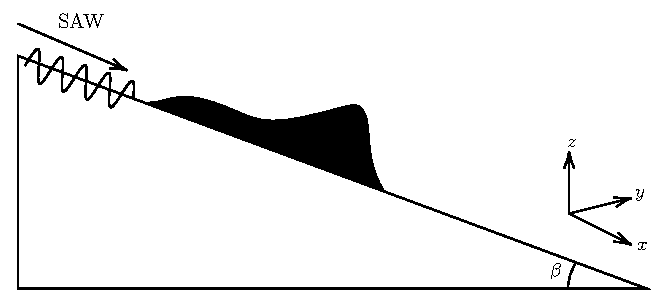
\includegraphics[width=\textwidth]{images/report/samp_diagram.pdf}
    \caption{A simplified sketch of a fluid flowing down a plane inclined at an angle $\beta$. The SAW travels
    from left to right, and the surface of the plane is described by the topography function $\func{s}{x, y} = 0$.}
    \label{fig:diagram}
\end{figure}

\section{Governing Equation} \label{sec:gov_eq}

\subsection{Lubrication Approximation}
As shown in \cite{kondic2003instabilities}, if the Reynold's number is sufficiently low, the inertial terms of the Navier-Stokes equations 
can be ignored. Thus, under the effects of gravity and SAW streaming forces the lubrication approximation gives
\begin{gather}
    \grad_2 p = \mu \frac{\partial^2 \vect{v}}{\partial z^2} + \rho g \sin\theta \vect{i} - J\cexpz\vect{i}
    \label{eq:pressure_grad}\\
    \pderiv{p}{z} = -\rho g \cos\theta - J\alpha_1 \cexpz
    \label{eq:pressure_z}
\end{gather}
where $J = \rho \lrp{1 + \alpha_1^2}A^2\omega^2k_i$,  $\grad_2 = \lrp{\partial_x, \partial_y}$, 
and $\vect{v} = \lrp{u, v}$. 

\subsection{Boundary Conditions}
\subsubsection{Laplace-Young Boundary Condition}
The Laplace-Young boundary condition states that at the interface $z = \func{\phi}{x, y, t}$, the pressure is given by 
$\func{p}{\phi} = -\gamma \kappa + p_0$, where $\kappa$ is the curvature of the boundary, $\gamma$ is the surface tension, and $p_0$ is the atmospheric pressure. 
Thus, integrating \cref{eq:pressure_z} gives 
\begin{align}
    \nonumber \int_{\phi}^{z} \pderiv{p}{z} \; dz &=  \int_{\phi}^{z} -\rho g \cos \theta - J\alpha_1 \cexpz \; dz\\
    \nonumber \func{p}{z} - \func{p}{\phi} &= -\lrp{z - \phi} \rho g \cos \theta - \frac{J}{2k_i} \lrp{\cexpz - \cexpp}\\
    \func{p}{z} &= -\lrp{z - \phi}\rho g \cos \theta - \frac{J}{2k_i} \lrp{\cexpz - \cexpp} -\gamma \kappa + p_0.  
    \label{eq:laplace_young}
\end{align}
If we define 
\begin{align}
    \func{P}{x, y, t} = \phi \rho g \cos\theta + \frac{J}{2k_i} \cexpp - \gamma\kappa, 
    \label{eq:cap_P}
\end{align}
this simplifies \cref{eq:laplace_young} to 
\begin{align*}
    \func{p}{z} = P - z\rho g \cos\theta - \frac{J}{2k_i}\cexpz + p_0
\end{align*}
which further gives 
\begin{align}
    \grad_2 p %= \grad_2 \lrp{P - z\rho g \cos\theta - \frac{J}{2k_i}\cexpz + p_0}
    = \grad_2 \lrp{P - \frac{J}{2k_i}\cexpz}
    = \grad P - J\cexpz \vect{i}
    \label{eq:grad2_p_expanded}
\end{align}

\subsubsection{Further Boundary Conditions}
Further boundary conditions include 
\begin{gather}
    \evalat{\vect{v}}{z = s\lrp{x,y}} = \vect{0} 
    \label{eq:bound_noslip}\\
    \evalat[\Big]{\pderiv{\vect{v}}{z}}{z = \phi\lrp{x,y,t}} = \vect{0} 
    \label{eq:bound_stress}
\end{gather}
where \cref{eq:bound_noslip} is a no-slip BC along the surface $z = \func{s}{x,y}$ and \cref{eq:bound_stress}
enforces vanishing shear stresses along the fluid-air boundary $z = \func{\phi}{x,y,t}$. 

\subsection{Film Equation}
\subsubsection{Velocity Vector Equation}
Under the Laplace-Young BC and \cref{eq:grad2_p_expanded}, \cref{eq:pressure_grad} simplifies into 
\begin{align}
    \grad P = \mu \frac{\partial^2 \vect{v}}{\partial z^2} + \rho g \sin\theta \vect{i}. 
    \label{eq:pressure_grad_new}
\end{align}
Integrating \cref{eq:pressure_grad_new} twice with respect to $z$ and utilizing  
\cref{eq:bound_noslip} and \cref{eq:bound_stress} gives
\begin{align}
    \nonumber \int_{s}^{z}\int_{z}^{\phi} \pderivtwo{\vect{v}}{z} \; dzdz &= \frac{1}{\mu}\int_{s}^{z}\int_{z}^{\phi} \lrp{\grad P - \rho g \sin\theta\vect{i}} \; dzdz \\
    \nonumber \int_{s}^{z} \lrp{\evalat[\Big]{\pderiv{\vect{v}}{z}}{z = \phi} - \pderiv{\vect{v}}{z}} \; dz &= \frac{1}{\mu} \lrp{\grad P - \rho g \sin\theta\vect{i}} \int_{s}^{z}\lrp{\phi - z} \; dz\\
    \nonumber \int_{s}^{z} \pderiv{\vect{v}}{z} \; dz &= \frac{1}{\mu} \lrp{\grad P - \rho g \sin\theta\vect{i}} \int_{s}^{z} \lrp{z - \phi} \; dz\\
    \nonumber \vect{v} - \evalat{\vect{v}}{z = s} &= \frac{1}{\mu} \lrp{\grad P - \rho g \sin\theta\vect{i}}  \lrp{\frac{z^2}{2} - \phi z} \Bigg|_{s}^z\\
    \vect{v} &=\frac{1}{\mu} \lrp{\grad P - \rho g \sin\theta\vect{i}} \lrp{\frac{z^2}{2} - \phi z - \frac{s^2}{2} + \phi s}. 
    \label{eq:vel_vectv}
\end{align}

\subsubsection{Depth Averaged Velocity}
Averaging over the height removes the $z$ dependence of $\vect{v} = \lrp{u, v}$ and gives the equation 
\begin{align*}
    \bar{\vect{v}} = \frac{1}{h} \int_{s}^{\phi} \vect{v} \; dz.
    %\label{eq:vectv_bar_int}
\end{align*}
Solving this integral then gives 
\begin{align}
    \nonumber \bar{\vect{v}} &= \frac{1}{h} \int_{s}^{\phi} \frac{1}{\mu} \lrp{\grad P - \rho g \sin\theta\vect{i}} \lrp{\frac{z^2}{2} - \phi z - \frac{s^2}{2} + \phi s}  \; dz\\
    \nonumber &= \frac{1}{\mu h} \lrp{\grad P - \rho g \sin\theta\vect{i}} \lrp{\frac{z^3}{6} - \frac{\phi z^2}{2} - z\lrp{\frac{s^2}{2} - \phi s}} \Bigg|_{s}^{\phi}\\
    \nonumber &= \frac{1}{\mu h} \lrp{\grad P - \rho g \sin\theta\vect{i}} \lrp{-\frac{\phi^3}{3} + \phi^2s - \phi s^2 + \frac{s^3}{3}}\\
    \nonumber &=  \frac{1}{\mu h} \lrp{\grad P - \rho g \sin\theta\vect{i}} \lrp{-\frac{(h+s)^3}{3} + (h+s)^2s - (h+s) s^2 + \frac{s^3}{3}}\\
    &= -\frac{h^2}{3\mu} \lrp{\grad P - \rho g \sin\theta\vect{i}}.
    \label{eq:uv_bar}
\end{align}

\subsubsection{Conservation of Mass}
The conservation of mass, when depth-averaged, gives 
\begin{align}
    \pderiv{h}{t} + \grad \cdot \lrp{h\bar{\vect{v}}} = 0
\end{align}
which results in 
\begin{align}
    \nonumber \pderiv{h}{t} &= \frac{1}{3\mu} \grad \cdot \lrb{h^3 \lrp{\grad P - \rho g \sin \theta \vect{i}}}\\
    &= \frac{1}{3\mu} \grad \cdot \lrb{h^3 \lrp{\rho g \cos\theta \grad \phi - \gamma\grad\kappa - \rho g \sin \theta \vect{i} + \frac{J}{2k_i}\grad \cexpp }}. 
\end{align}
Approximating the curvature $\kappa \approx \grad^2 \phi$ then gives 
\begin{align}
    \nonumber \pderiv{h}{t} &= \frac{1}{3\mu} \grad \cdot \lrb{h^3 \lrp{\rho g \cos\theta \grad \phi - \gamma\grad\grad^2\phi - \rho g \sin \theta \vect{i} + \frac{J}{2k_i}\grad \cexpp}}\\
    &= \frac{1}{3\mu} \lrb{ \grad \cdot \lrb{\rho g \cos \theta h^3 \grad \phi} - \grad \cdot \lrb{\gamma h^3 \grad\grad^2\phi} - \rho g \sin\theta \pderiv{h^3}{x} + \grad \cdot \lrb{\frac{J}{2k_i}h^3\grad \cexpp}}.
    \label{eq:thin_film_dim}
\end{align}

\subsection{Dimensionless Form}
Scale the in-plane coordinates and time by 
\begin{gather}
    \bar{x} = \frac{x}{x_c}, \quad \bar{y} = \frac{y}{x_c}, \quad \bar{z} = \frac{z}{h_c}, \quad \bar{t} = \frac{t}{t_c}. 
    \label{eq:coord_time_scales}
\end{gather}
where an overline denotes a non-dimensional quantity. From these scales, we get that  
\begin{gather*}
    k_i = \frac{\bar{k_i}}{x_c}, \quad \omega = \frac{\bar{\omega}}{t_c}, \quad A = \bar{A}h_c
\end{gather*}
and thus that 
\begin{align}
    J = \rho \lrp{1 + \alpha_1^2}  \bar{A}^2 h_c^2 \frac{\bar{\omega}^2 \bar{k_i}}{t_c^2 x_c} = \frac{\rho \eta h_c^2}{t_c^2 x_c}
    \label{eq:J_nondim}
\end{align}
where $\eta = \lrp{1 + \alpha_1^2}  \bar{A}^2 \bar{\omega}^2 \bar{k_i}$ is non-dimensional. Substituting the scales in 
\cref{eq:coord_time_scales} and \cref{eq:J_nondim} into \cref{eq:thin_film_dim} and removing any bars gives 
\begin{multline}
    \frac{h_c}{t_c} \pderiv{h}{t} = \frac{1}{3\mu} \lrb{
        \frac{h_c^4}{x_c^2} \rho g \cos \theta \grad \cdot \lrb{h^3\grad\phi} - 
        \frac{\gamma h_c^4}{x_c^4} \grad \cdot \lrb{h^3 \grad \grad^2 \phi} - 
        \frac{h_c^3}{x_c} \rho g \sin\theta \pderiv{h^3}{x}
    }\\
    + \frac{1}{3\mu} \lrb{ 
        \frac{\eta \rho h_c^5}{2k_i t_c^2 x_c^2} \grad \cdot \lrb{h^3 \grad e^{2k_i \lrp{x + \alpha_1 \phi \lrp{h_c/x_c}}}}
    }.
    \label{eq:nondim_first}
\end{multline}
By virtue of the fact that we are dealing with a thin film, $h_c \ll x_c$. Additionally, by definition
$\alpha_1 = -i \alpha$ where 
\begin{equation*}
    \alpha = \lrp{1 - \lrp{V_r/V_w}^2}^{1/2}
\end{equation*}
with $V_r$ and $V_w$ being the velocity of the SAW in the solid substrate and fluid, respectively. Since 
$V_r > V_w$
\begin{equation*}
    \alpha = i \lrp{\lrp{V_r/V_w}^2 - 1}^{1/2} \quad \rightarrow \quad \alpha_1 = \lrp{\lrp{V_r/V_w}^2 - 1}^{1/2}
\end{equation*}
which is real and $\bigo{1}$. Thus, we can ignore any component of the exponent 
that is multiplied by $\alpha_1$ and $h_c / x_c$, which simplifies \cref{eq:nondim_first} to 
\begin{align}
    \nonumber \frac{h_c}{t_c} \pderiv{h}{t} &= \frac{1}{3\mu} \lrb{
        \frac{h_c^4}{x_c^2} \rho g \cos \theta \grad \cdot \lrb{h^3\grad\phi} - 
        \frac{\gamma h_c^4}{x_c^4} \grad \cdot \lrb{h^3 \grad \grad^2 \phi} - 
        \frac{h_c^3}{x_c} \rho g \sin\theta \pderiv{h^3}{x} + 
        \frac{\eta h_c^5}{2k_i t_c^2 x_c^2} \grad \cdot \lrb{h^3 \grad e^{2k_i x}}
        %\frac{\eta h_c^5}{t_c^2 x_c^2} \pderiv{}{x} \lrb{h^3 \grad e^{2k_i x}}. 
    }\\
    \nonumber &= \frac{\gamma h_c^4}{3\mu x_c^4} \lrb{
        \frac{x_c^2 \rho g}{\gamma} \cos \theta \grad \cdot \lrb{h^3\grad\phi} - 
        \grad \cdot \lrb{h^3 \grad \grad^2 \phi} - 
        \frac{x_c^3}{\gamma h_c} \sin\theta \pderiv{h^3}{x} + 
        \frac{\eta \rho x_c^2 h_c}{\gamma t_c^2} \pderiv{}{x} \lrb{h^3 e^{2k_i x}}
    }\\
    \pderiv{h}{t} &= \frac{\gamma h_c^3}{3\mu x_c^4 t_c} \lrb{
        \frac{x_c^2 \rho g}{\gamma} \cos \theta \grad \cdot \lrb{h^3\grad\phi} - 
        \grad \cdot \lrb{h^3 \grad \grad^2 \phi} - 
        \frac{x_c^3}{\gamma h_c} \sin\theta \pderiv{h^3}{x} + 
        \frac{\eta \rho x_c^2 h_c}{\gamma t_c^2} \pderiv{}{x} \lrb{h^3 e^{2k_i x}}
    }.
    \label{eq:nondim_sec}
\end{align}
Choose $x_c$ and $t_c$ such that 
\begin{align}
    x_c = \lrp{\frac{\gamma h_c}{\rho g}}^{1/3}, \quad t_c = \frac{3\mu x_c}{h_c^2 \rho g}.
    \label{eq:x_and_t_scales}
\end{align}
Substituting these scales into \cref{eq:nondim_sec} yields
\begin{align}
    \pderiv{h}{t} = \lrp{\frac{h_c^2 \rho g}{\gamma}}^{1/3} \cos\theta \grad \cdot \lrb{ h^3 \grad \phi } - 
    \grad \cdot \lrb{h^3 \grad\grad^2\phi } - 
    \sin\theta \pderiv{h^3}{x} + 
    \frac{\eta \rho x_c^2 h_c}{\gamma t_c^2} \pderiv{}{x} \lrb{h^3 e^{2k_i x}}.
    \label{eq:nondim_third}
\end{align}  
The velocity scale is chosen naturally as $U = x_c/t_c = h_c^2\rho g/3\mu$,
which allows us to additionally define the capillary number $\mathrm{Ca} = \mu U / \gamma = h_c^2\rho g/3\gamma$
and Weber number $\mathrm{We} = \rho U^2 h_c / \gamma = \rho x_c^2 h_c / \gamma t_c^2$, both of which
are non-dimensional quantities. Hence, 
\cref{eq:nondim_third} simplifies to 
\begin{align}
    \pderiv{h}{t} = \lrp{3\mathrm{Ca}}^{1/3} \cos\theta \grad \cdot \lrb{ h^3 \grad \phi } - 
    \grad \cdot \lrb{h^3 \grad\grad^2\phi } - 
    \sin\theta \pderiv{h^3}{x} + 
    \eta \mathrm{We} \pderiv{}{x} \lrb{h^3 e^{2k_i x}}.
    \label{eq:nondim_fourth}
\end{align}  
If we further define 
\begin{equation*}
    D = \lrp{3\mathrm{Ca}}^{1/3}, \quad C = \eta \mathrm{We}
\end{equation*}
then we get a final equation 
\begin{align}
    \pderiv{h}{t} = D \cos\theta \grad \cdot \lrb{ h^3 \grad \phi } - 
    \grad \cdot \lrb{h^3 \grad\grad^2\phi } - 
    \sin\theta \pderiv{h^3}{x} + 
    C \pderiv{}{x} \lrb{h^3 e^{2k_i x}}.
    \label{eq:nondim_final}
\end{align}  
 
\section{Method of Solution} \label{sec:method_of_sol}
\subsection{Spatial Discretization}
If we define the domain of interest as $\lrb{0, L_x}$, we can discretize the 
domain into points $x_j = j\Delta x$ for $j = 0, \ldots, N_x$ where 
$\Delta x = L_x / N_x$ and $N_x$ is the number of grid points excluding the origin. 
If we further define $\func{h_j}{t} = \func{h}{x_j, t}$, we can discretize 
\cref{eq:two_dim_final} into a system of ordinary differential equations of the form 
\begin{equation}
    \deriv{h_j}{t} = f_j = \mathrm{Bo}\cos \beta f_j^{(1)} - f_j^{(2)} -  \frac{\mathrm{Bo}}{\varepsilon} \sin \beta f_j^{(3)} +  
    \frac{k_i \lrp{1 + \alpha_1^2} \mathrm{We_{ac}}}{\varepsilon} f_j^{(4)}, \quad j = 0, \ldots, N_x
    \label{eq:ode_sys}
\end{equation}
where $f_j^{(k)}$ is the discretization of the $k$-th term in
the right-hand side of \cref{eq:two_dim_final}. Because the governing equation 
contains high order derivatives, the discretization used for certain components 
needs special attention in order to not lead to a large computational stencil.

\subsubsection{Fourth-Order Term}
Following the method outlined in \cite{kondic2003instabilities}, discretizing the fourth order term (i.e.\! $f_j^{(2)}$) can be done by a combination
of forward and backward differences. If we define 
\begin{align*}
    h_{x, j} = \frac{h_{j+1} - h_j}{\Delta x} \quad \quad \quad h_{\overline{x}, j} = \frac{h_{j} - h_{j-1}}{\Delta x}
\end{align*}
as the forward and backward differences, respectively, then a possible discretization is 
\begin{equation}
    f_j^{\lrp{2}} = \lrp{\func{a}{h_{i-1}, h_i} \phi_{\overline{x}x\overline{x}}}_{x}
    \label{eq:f2_disc}
\end{equation}
where $\func{a}{j_1, j_2} = \frac{1}{2} \lrp{{j_1}^3 + {j_2}^3}$. This discretization leads to a 
second order approximation that has a five point stencil, which is better than the seven point stencil
that would result from using a central differencing scheme. 

\subsubsection{Lower Order Terms}


%\begin{figure}[h]  
%    \centering
%    \resizebox{.75\linewidth}{!}{\begin{tikzpicture}[/tikz/background rectangle/.style={fill={rgb,1:red,1.0;green,1.0;blue,1.0}, draw opacity={1.0}}, show background rectangle]
\begin{axis}[point meta max={nan}, point meta min={nan}, legend cell align={left}, legend columns={1}, title={Fluid profile at $\delta t = 2$ intervals}, title style={at={{(0.5,1)}}, anchor={south}, font={{\fontsize{14 pt}{18.2 pt}\selectfont}}, color={rgb,1:red,0.0;green,0.0;blue,0.0}, draw opacity={1.0}, rotate={0.0}}, legend style={color={rgb,1:red,0.0;green,0.0;blue,0.0}, draw opacity={1.0}, line width={1}, solid, fill={rgb,1:red,1.0;green,1.0;blue,1.0}, fill opacity={1.0}, text opacity={1.0}, font={{\fontsize{8 pt}{10.4 pt}\selectfont}}, text={rgb,1:red,0.0;green,0.0;blue,0.0}, cells={anchor={center}}, at={(1.02, 1)}, anchor={north west}}, axis background/.style={fill={rgb,1:red,1.0;green,1.0;blue,1.0}, opacity={1.0}}, anchor={north west}, xshift={1.0mm}, yshift={-1.0mm}, clip mode={individual}, width={150.4mm}, height={99.6mm}, scaled x ticks={false}, xlabel={Dimensionless length $x$}, x tick style={color={rgb,1:red,0.0;green,0.0;blue,0.0}, opacity={1.0}}, x tick label style={color={rgb,1:red,0.0;green,0.0;blue,0.0}, opacity={1.0}, rotate={0}}, xlabel style={at={(ticklabel cs:0.5)}, anchor=near ticklabel, at={{(ticklabel cs:0.5)}}, anchor={near ticklabel}, font={{\fontsize{11 pt}{14.3 pt}\selectfont}}, color={rgb,1:red,0.0;green,0.0;blue,0.0}, draw opacity={1.0}, rotate={0.0}}, xmajorgrids={false}, xmin={0}, xmax={40}, xtick={{0.0,10.0,20.0,30.0,40.0}}, xticklabels={{$0$,$10$,$20$,$30$,$40$}}, xtick align={inside}, xticklabel style={font={{\fontsize{8 pt}{10.4 pt}\selectfont}}, color={rgb,1:red,0.0;green,0.0;blue,0.0}, draw opacity={1.0}, rotate={0.0}}, x grid style={color={rgb,1:red,0.0;green,0.0;blue,0.0}, draw opacity={0.1}, line width={0.5}, solid}, axis x line*={left}, x axis line style={color={rgb,1:red,0.0;green,0.0;blue,0.0}, draw opacity={1.0}, line width={1}, solid}, scaled y ticks={false}, ylabel={Dimensionless free surface height $\phi$}, y tick style={color={rgb,1:red,0.0;green,0.0;blue,0.0}, opacity={1.0}}, y tick label style={color={rgb,1:red,0.0;green,0.0;blue,0.0}, opacity={1.0}, rotate={0}}, ylabel style={at={(ticklabel cs:0.5)}, anchor=near ticklabel, at={{(ticklabel cs:0.5)}}, anchor={near ticklabel}, font={{\fontsize{11 pt}{14.3 pt}\selectfont}}, color={rgb,1:red,0.0;green,0.0;blue,0.0}, draw opacity={1.0}, rotate={0.0}}, ymajorgrids={false}, ymin={0}, ymax={9.73932989159924}, ytick={{0.0,2.0,4.0,6.0,8.0}}, yticklabels={{$0$,$2$,$4$,$6$,$8$}}, ytick align={inside}, yticklabel style={font={{\fontsize{8 pt}{10.4 pt}\selectfont}}, color={rgb,1:red,0.0;green,0.0;blue,0.0}, draw opacity={1.0}, rotate={0.0}}, y grid style={color={rgb,1:red,0.0;green,0.0;blue,0.0}, draw opacity={0.1}, line width={0.5}, solid}, axis y line*={left}, y axis line style={color={rgb,1:red,0.0;green,0.0;blue,0.0}, draw opacity={1.0}, line width={1}, solid}, colorbar={false}]
    \addplot[color={rgb,1:red,0.0;green,0.0;blue,0.0}, name path={6eca9dd9-ef34-4e43-ba15-06d3ff9281f9}, draw opacity={1.0}, line width={1}, solid]
        table[row sep={\\}]
        {
            \\
            0.0  0.0  \\
            0.05  0.0  \\
            0.1  0.0  \\
            0.15  0.0  \\
            0.2  0.0  \\
            0.25  0.0  \\
            0.3  0.0  \\
            0.35  0.0  \\
            0.4  0.0  \\
            0.45  0.0  \\
            0.5  0.0  \\
            0.55  0.0  \\
            0.6  0.0  \\
            0.65  0.0  \\
            0.7  0.0  \\
            0.75  0.0  \\
            0.8  0.0  \\
            0.85  0.0  \\
            0.9  0.0  \\
            0.95  0.0  \\
            1.0  0.0  \\
            1.05  0.0  \\
            1.1  0.0  \\
            1.15  0.0  \\
            1.2  0.0  \\
            1.25  0.0  \\
            1.3  0.0  \\
            1.35  0.0  \\
            1.4  0.0  \\
            1.45  0.0  \\
            1.5  0.0  \\
            1.55  0.0  \\
            1.6  0.0  \\
            1.65  0.0  \\
            1.7  0.0  \\
            1.75  0.0  \\
            1.8  0.0  \\
            1.85  0.0  \\
            1.9  0.0  \\
            1.95  0.0  \\
            2.0  0.0  \\
            2.05  0.0  \\
            2.1  0.0  \\
            2.15  0.0  \\
            2.2  0.0  \\
            2.25  0.0  \\
            2.3  0.0  \\
            2.35  0.0  \\
            2.4  0.0  \\
            2.45  0.0  \\
            2.5  0.0  \\
            2.55  0.0  \\
            2.6  0.0  \\
            2.65  0.0  \\
            2.7  0.0  \\
            2.75  0.0  \\
            2.8  0.0  \\
            2.85  0.0  \\
            2.9  0.0  \\
            2.95  0.0  \\
            3.0  0.0  \\
            3.05  0.0  \\
            3.1  0.0  \\
            3.15  0.0  \\
            3.2  0.0  \\
            3.25  0.0  \\
            3.3  0.0  \\
            3.35  0.0  \\
            3.4  0.0  \\
            3.45  0.0  \\
            3.5  0.0  \\
            3.55  0.0  \\
            3.6  0.0  \\
            3.65  0.0  \\
            3.7  0.0  \\
            3.75  0.0  \\
            3.8  0.0  \\
            3.85  0.0  \\
            3.9  0.0  \\
            3.95  0.0  \\
            4.0  0.0  \\
            4.05  0.0  \\
            4.1  0.0  \\
            4.15  0.0  \\
            4.2  0.0  \\
            4.25  0.0  \\
            4.3  0.0  \\
            4.35  0.0  \\
            4.4  0.0  \\
            4.45  0.0  \\
            4.5  0.0  \\
            4.55  0.0  \\
            4.6  0.0  \\
            4.65  0.0  \\
            4.7  0.0  \\
            4.75  0.0  \\
            4.8  0.0  \\
            4.85  0.0  \\
            4.9  0.0  \\
            4.95  0.0  \\
            5.0  0.0  \\
            5.05  0.0  \\
            5.1  0.0  \\
            5.15  0.0  \\
            5.2  0.0  \\
            5.25  0.0  \\
            5.3  0.0  \\
            5.35  0.0  \\
            5.4  0.0  \\
            5.45  0.0  \\
            5.5  0.0  \\
            5.55  0.0  \\
            5.6  0.0  \\
            5.65  0.0  \\
            5.7  0.0  \\
            5.75  0.0  \\
            5.8  0.0  \\
            5.85  0.0  \\
            5.9  0.0  \\
            5.95  0.0  \\
            6.0  0.0  \\
            6.05  0.0  \\
            6.1  0.0  \\
            6.15  0.0  \\
            6.2  0.0  \\
            6.25  0.0  \\
            6.3  0.0  \\
            6.35  0.0  \\
            6.4  0.0  \\
            6.45  0.0  \\
            6.5  0.0  \\
            6.55  0.0  \\
            6.6  0.0  \\
            6.65  0.0  \\
            6.7  0.0  \\
            6.75  0.0  \\
            6.8  0.0  \\
            6.85  0.0  \\
            6.9  0.0  \\
            6.95  0.0  \\
            7.0  0.0  \\
            7.05  0.0  \\
            7.1  0.0  \\
            7.15  0.0  \\
            7.2  0.0  \\
            7.25  0.0  \\
            7.3  0.0  \\
            7.35  0.0  \\
            7.4  0.0  \\
            7.45  0.0  \\
            7.5  0.0  \\
            7.55  0.0  \\
            7.6  0.0  \\
            7.65  0.0  \\
            7.7  0.0  \\
            7.75  0.0  \\
            7.8  0.0  \\
            7.85  0.0  \\
            7.9  0.0  \\
            7.95  0.0  \\
            8.0  0.0  \\
            8.05  0.0  \\
            8.1  0.0  \\
            8.15  0.0  \\
            8.2  0.0  \\
            8.25  0.0  \\
            8.3  0.0  \\
            8.35  0.0  \\
            8.4  0.0  \\
            8.45  0.0  \\
            8.5  0.0  \\
            8.55  0.0  \\
            8.6  0.0  \\
            8.65  0.0  \\
            8.7  0.0  \\
            8.75  0.0  \\
            8.8  0.0  \\
            8.85  0.0  \\
            8.9  0.0  \\
            8.95  0.0  \\
            9.0  0.0  \\
            9.05  0.0  \\
            9.1  0.0  \\
            9.15  0.0  \\
            9.2  0.0  \\
            9.25  0.0  \\
            9.3  0.0  \\
            9.35  0.0  \\
            9.4  0.0  \\
            9.45  0.0  \\
            9.5  0.0  \\
            9.55  0.0  \\
            9.6  0.0  \\
            9.65  0.0  \\
            9.7  0.0  \\
            9.75  0.0  \\
            9.8  0.0  \\
            9.85  0.0  \\
            9.9  0.0  \\
            9.95  0.0  \\
            10.0  0.0  \\
            10.05  0.0  \\
            10.1  0.0  \\
            10.15  0.0  \\
            10.2  0.0  \\
            10.25  0.0  \\
            10.3  0.0  \\
            10.35  0.0  \\
            10.4  0.0  \\
            10.45  0.0  \\
            10.5  0.0  \\
            10.55  0.0  \\
            10.6  0.0  \\
            10.65  0.0  \\
            10.7  0.0  \\
            10.75  0.0  \\
            10.8  0.0  \\
            10.85  0.0  \\
            10.9  0.0  \\
            10.95  0.0  \\
            11.0  0.0  \\
            11.05  0.0  \\
            11.1  0.0  \\
            11.15  0.0  \\
            11.2  0.0  \\
            11.25  0.0  \\
            11.3  0.0  \\
            11.35  0.0  \\
            11.4  0.0  \\
            11.45  0.0  \\
            11.5  0.0  \\
            11.55  0.0  \\
            11.6  0.0  \\
            11.65  0.0  \\
            11.7  0.0  \\
            11.75  0.0  \\
            11.8  0.0  \\
            11.85  0.0  \\
            11.9  0.0  \\
            11.95  0.0  \\
            12.0  0.0  \\
            12.05  0.0  \\
            12.1  0.0  \\
            12.15  0.0  \\
            12.2  0.0  \\
            12.25  0.0  \\
            12.3  0.0  \\
            12.35  0.0  \\
            12.4  0.0  \\
            12.45  0.0  \\
            12.5  0.0  \\
            12.55  0.0  \\
            12.6  0.0  \\
            12.65  0.0  \\
            12.7  0.0  \\
            12.75  0.0  \\
            12.8  0.0  \\
            12.85  0.0  \\
            12.9  0.0  \\
            12.95  0.0  \\
            13.0  0.0  \\
            13.05  0.0  \\
            13.1  0.0  \\
            13.15  0.0  \\
            13.2  0.0  \\
            13.25  0.0  \\
            13.3  0.0  \\
            13.35  0.0  \\
            13.4  0.0  \\
            13.45  0.0  \\
            13.5  0.0  \\
            13.55  0.0  \\
            13.6  0.0  \\
            13.65  0.0  \\
            13.7  0.0  \\
            13.75  0.0  \\
            13.8  0.0  \\
            13.85  0.0  \\
            13.9  0.0  \\
            13.95  0.0  \\
            14.0  0.0  \\
            14.05  0.0  \\
            14.1  0.0  \\
            14.15  0.0  \\
            14.2  0.0  \\
            14.25  0.0  \\
            14.3  0.0  \\
            14.35  0.0  \\
            14.4  0.0  \\
            14.45  0.0  \\
            14.5  0.0  \\
            14.55  0.0  \\
            14.6  0.0  \\
            14.65  0.0  \\
            14.7  0.0  \\
            14.75  0.0  \\
            14.8  0.0  \\
            14.85  0.0  \\
            14.9  0.0  \\
            14.95  0.0  \\
            15.0  0.0  \\
            15.05  0.0  \\
            15.1  0.0  \\
            15.15  0.0  \\
            15.2  0.0  \\
            15.25  0.0  \\
            15.3  0.0  \\
            15.35  0.0  \\
            15.4  0.0  \\
            15.45  0.0  \\
            15.5  0.0  \\
            15.55  0.0  \\
            15.6  0.0  \\
            15.65  0.0  \\
            15.7  0.0  \\
            15.75  0.0  \\
            15.8  0.0  \\
            15.85  0.0  \\
            15.9  0.0  \\
            15.95  0.0  \\
            16.0  0.0  \\
            16.05  0.0  \\
            16.1  0.0  \\
            16.15  0.0  \\
            16.2  0.0  \\
            16.25  0.0  \\
            16.3  0.0  \\
            16.35  0.0  \\
            16.4  0.0  \\
            16.45  0.0  \\
            16.5  0.0  \\
            16.55  0.0  \\
            16.6  0.0  \\
            16.65  0.0  \\
            16.7  0.0  \\
            16.75  0.0  \\
            16.8  0.0  \\
            16.85  0.0  \\
            16.9  0.0  \\
            16.95  0.0  \\
            17.0  0.0  \\
            17.05  0.0  \\
            17.1  0.0  \\
            17.15  0.0  \\
            17.2  0.0  \\
            17.25  0.0  \\
            17.3  0.0  \\
            17.35  0.0  \\
            17.4  0.0  \\
            17.45  0.0  \\
            17.5  0.0  \\
            17.55  0.0  \\
            17.6  0.0  \\
            17.65  0.0  \\
            17.7  0.0  \\
            17.75  0.0  \\
            17.8  0.0  \\
            17.85  0.0  \\
            17.9  0.0  \\
            17.95  0.0  \\
            18.0  0.0  \\
            18.05  0.0  \\
            18.1  0.0  \\
            18.15  0.0  \\
            18.2  0.0  \\
            18.25  0.0  \\
            18.3  0.0  \\
            18.35  0.0  \\
            18.4  0.0  \\
            18.45  0.0  \\
            18.5  0.0  \\
            18.55  0.0  \\
            18.6  0.0  \\
            18.65  0.0  \\
            18.7  0.0  \\
            18.75  0.0  \\
            18.8  0.0  \\
            18.85  0.0  \\
            18.9  0.0  \\
            18.95  0.0  \\
            19.0  0.0  \\
            19.05  0.0  \\
            19.1  0.0  \\
            19.15  0.0  \\
            19.2  0.0  \\
            19.25  0.0  \\
            19.3  0.0  \\
            19.35  0.0  \\
            19.4  0.0  \\
            19.45  0.0  \\
            19.5  0.0  \\
            19.55  0.0  \\
            19.6  0.0  \\
            19.65  0.0  \\
            19.7  0.0  \\
            19.75  0.0  \\
            19.8  0.0  \\
            19.85  0.0  \\
            19.9  0.0  \\
            19.95  0.0  \\
            20.0  0.0  \\
            20.05  0.0  \\
            20.1  0.0  \\
            20.15  0.0  \\
            20.2  0.0  \\
            20.25  0.0  \\
            20.3  0.0  \\
            20.35  0.0  \\
            20.4  0.0  \\
            20.45  0.0  \\
            20.5  0.0  \\
            20.55  0.0  \\
            20.6  0.0  \\
            20.65  0.0  \\
            20.7  0.0  \\
            20.75  0.0  \\
            20.8  0.0  \\
            20.85  0.0  \\
            20.9  0.0  \\
            20.95  0.0  \\
            21.0  0.0  \\
            21.05  0.0  \\
            21.1  0.0  \\
            21.15  0.0  \\
            21.2  0.0  \\
            21.25  0.0  \\
            21.3  0.0  \\
            21.35  0.0  \\
            21.4  0.0  \\
            21.45  0.0  \\
            21.5  0.0  \\
            21.55  0.0  \\
            21.6  0.0  \\
            21.65  0.0  \\
            21.7  0.0  \\
            21.75  0.0  \\
            21.8  0.0  \\
            21.85  0.0  \\
            21.9  0.0  \\
            21.95  0.0  \\
            22.0  0.0  \\
            22.05  0.0  \\
            22.1  0.0  \\
            22.15  0.0  \\
            22.2  0.0  \\
            22.25  0.0  \\
            22.3  0.0  \\
            22.35  0.0  \\
            22.4  0.0  \\
            22.45  0.0  \\
            22.5  0.0  \\
            22.55  0.0  \\
            22.6  0.0  \\
            22.65  0.0  \\
            22.7  0.0  \\
            22.75  0.0  \\
            22.8  0.0  \\
            22.85  0.0  \\
            22.9  0.0  \\
            22.95  0.0  \\
            23.0  0.0  \\
            23.05  0.0  \\
            23.1  0.0  \\
            23.15  0.0  \\
            23.2  0.0  \\
            23.25  0.0  \\
            23.3  0.0  \\
            23.35  0.0  \\
            23.4  0.0  \\
            23.45  0.0  \\
            23.5  0.0  \\
            23.55  0.0  \\
            23.6  0.0  \\
            23.65  0.0  \\
            23.7  0.0  \\
            23.75  0.0  \\
            23.8  0.0  \\
            23.85  0.0  \\
            23.9  0.0  \\
            23.95  0.0  \\
            24.0  0.0  \\
            24.05  0.0  \\
            24.1  0.0  \\
            24.15  0.0  \\
            24.2  0.0  \\
            24.25  0.0  \\
            24.3  0.0  \\
            24.35  0.0  \\
            24.4  0.0  \\
            24.45  0.0  \\
            24.5  0.0  \\
            24.55  0.0  \\
            24.6  0.0  \\
            24.65  0.0  \\
            24.7  0.0  \\
            24.75  0.0  \\
            24.8  0.0  \\
            24.85  0.0  \\
            24.9  0.0  \\
            24.95  0.0  \\
            25.0  0.0  \\
            25.05  0.0  \\
            25.1  0.0  \\
            25.15  0.0  \\
            25.2  0.0  \\
            25.25  0.0  \\
            25.3  0.0  \\
            25.35  0.0  \\
            25.4  0.0  \\
            25.45  0.0  \\
            25.5  0.0  \\
            25.55  0.0  \\
            25.6  0.0  \\
            25.65  0.0  \\
            25.7  0.0  \\
            25.75  0.0  \\
            25.8  0.0  \\
            25.85  0.0  \\
            25.9  0.0  \\
            25.95  0.0  \\
            26.0  0.0  \\
            26.05  0.0  \\
            26.1  0.0  \\
            26.15  0.0  \\
            26.2  0.0  \\
            26.25  0.0  \\
            26.3  0.0  \\
            26.35  0.0  \\
            26.4  0.0  \\
            26.45  0.0  \\
            26.5  0.0  \\
            26.55  0.0  \\
            26.6  0.0  \\
            26.65  0.0  \\
            26.7  0.0  \\
            26.75  0.0  \\
            26.8  0.0  \\
            26.85  0.0  \\
            26.9  0.0  \\
            26.95  0.0  \\
            27.0  0.0  \\
            27.05  0.0  \\
            27.1  0.0  \\
            27.15  0.0  \\
            27.2  0.0  \\
            27.25  0.0  \\
            27.3  0.0  \\
            27.35  0.0  \\
            27.4  0.0  \\
            27.45  0.0  \\
            27.5  0.0  \\
            27.55  0.0  \\
            27.6  0.0  \\
            27.65  0.0  \\
            27.7  0.0  \\
            27.75  0.0  \\
            27.8  0.0  \\
            27.85  0.0  \\
            27.9  0.0  \\
            27.95  0.0  \\
            28.0  0.0  \\
            28.05  0.0  \\
            28.1  0.0  \\
            28.15  0.0  \\
            28.2  0.0  \\
            28.25  0.0  \\
            28.3  0.0  \\
            28.35  0.0  \\
            28.4  0.0  \\
            28.45  0.0  \\
            28.5  0.0  \\
            28.55  0.0  \\
            28.6  0.0  \\
            28.65  0.0  \\
            28.7  0.0  \\
            28.75  0.0  \\
            28.8  0.0  \\
            28.85  0.0  \\
            28.9  0.0  \\
            28.95  0.0  \\
            29.0  0.0  \\
            29.05  0.0  \\
            29.1  0.0  \\
            29.15  0.0  \\
            29.2  0.0  \\
            29.25  0.0  \\
            29.3  0.0  \\
            29.35  0.0  \\
            29.4  0.0  \\
            29.45  0.0  \\
            29.5  0.0  \\
            29.55  0.0  \\
            29.6  0.0  \\
            29.65  0.0  \\
            29.7  0.0  \\
            29.75  0.0  \\
            29.8  0.0  \\
            29.85  0.0  \\
            29.9  0.0  \\
            29.95  0.0  \\
            30.0  0.0  \\
            30.05  0.0  \\
            30.1  0.0  \\
            30.15  0.0  \\
            30.2  0.0  \\
            30.25  0.0  \\
            30.3  0.0  \\
            30.35  0.0  \\
            30.4  0.0  \\
            30.45  0.0  \\
            30.5  0.0  \\
            30.55  0.0  \\
            30.6  0.0  \\
            30.65  0.0  \\
            30.7  0.0  \\
            30.75  0.0  \\
            30.8  0.0  \\
            30.85  0.0  \\
            30.9  0.0  \\
            30.95  0.0  \\
            31.0  0.0  \\
            31.05  0.0  \\
            31.1  0.0  \\
            31.15  0.0  \\
            31.2  0.0  \\
            31.25  0.0  \\
            31.3  0.0  \\
            31.35  0.0  \\
            31.4  0.0  \\
            31.45  0.0  \\
            31.5  0.0  \\
            31.55  0.0  \\
            31.6  0.0  \\
            31.65  0.0  \\
            31.7  0.0  \\
            31.75  0.0  \\
            31.8  0.0  \\
            31.85  0.0  \\
            31.9  0.0  \\
            31.95  0.0  \\
            32.0  0.0  \\
            32.05  0.0  \\
            32.1  0.0  \\
            32.15  0.0  \\
            32.2  0.0  \\
            32.25  0.0  \\
            32.3  0.0  \\
            32.35  0.0  \\
            32.4  0.0  \\
            32.45  0.0  \\
            32.5  0.0  \\
            32.55  0.0  \\
            32.6  0.0  \\
            32.65  0.0  \\
            32.7  0.0  \\
            32.75  0.0  \\
            32.8  0.0  \\
            32.85  0.0  \\
            32.9  0.0  \\
            32.95  0.0  \\
            33.0  0.0  \\
            33.05  0.0  \\
            33.1  0.0  \\
            33.15  0.0  \\
            33.2  0.0  \\
            33.25  0.0  \\
            33.3  0.0  \\
            33.35  0.0  \\
            33.4  0.0  \\
            33.45  0.0  \\
            33.5  0.0  \\
            33.55  0.0  \\
            33.6  0.0  \\
            33.65  0.0  \\
            33.7  0.0  \\
            33.75  0.0  \\
            33.8  0.0  \\
            33.85  0.0  \\
            33.9  0.0  \\
            33.95  0.0  \\
            34.0  0.0  \\
            34.05  0.0  \\
            34.1  0.0  \\
            34.15  0.0  \\
            34.2  0.0  \\
            34.25  0.0  \\
            34.3  0.0  \\
            34.35  0.0  \\
            34.4  0.0  \\
            34.45  0.0  \\
            34.5  0.0  \\
            34.55  0.0  \\
            34.6  0.0  \\
            34.65  0.0  \\
            34.7  0.0  \\
            34.75  0.0  \\
            34.8  0.0  \\
            34.85  0.0  \\
            34.9  0.0  \\
            34.95  0.0  \\
            35.0  0.0  \\
            35.05  0.0  \\
            35.1  0.0  \\
            35.15  0.0  \\
            35.2  0.0  \\
            35.25  0.0  \\
            35.3  0.0  \\
            35.35  0.0  \\
            35.4  0.0  \\
            35.45  0.0  \\
            35.5  0.0  \\
            35.55  0.0  \\
            35.6  0.0  \\
            35.65  0.0  \\
            35.7  0.0  \\
            35.75  0.0  \\
            35.8  0.0  \\
            35.85  0.0  \\
            35.9  0.0  \\
            35.95  0.0  \\
            36.0  0.0  \\
            36.05  0.0  \\
            36.1  0.0  \\
            36.15  0.0  \\
            36.2  0.0  \\
            36.25  0.0  \\
            36.3  0.0  \\
            36.35  0.0  \\
            36.4  0.0  \\
            36.45  0.0  \\
            36.5  0.0  \\
            36.55  0.0  \\
            36.6  0.0  \\
            36.65  0.0  \\
            36.7  0.0  \\
            36.75  0.0  \\
            36.8  0.0  \\
            36.85  0.0  \\
            36.9  0.0  \\
            36.95  0.0  \\
            37.0  0.0  \\
            37.05  0.0  \\
            37.1  0.0  \\
            37.15  0.0  \\
            37.2  0.0  \\
            37.25  0.0  \\
            37.3  0.0  \\
            37.35  0.0  \\
            37.4  0.0  \\
            37.45  0.0  \\
            37.5  0.0  \\
            37.55  0.0  \\
            37.6  0.0  \\
            37.65  0.0  \\
            37.7  0.0  \\
            37.75  0.0  \\
            37.8  0.0  \\
            37.85  0.0  \\
            37.9  0.0  \\
            37.95  0.0  \\
            38.0  0.0  \\
            38.05  0.0  \\
            38.1  0.0  \\
            38.15  0.0  \\
            38.2  0.0  \\
            38.25  0.0  \\
            38.3  0.0  \\
            38.35  0.0  \\
            38.4  0.0  \\
            38.45  0.0  \\
            38.5  0.0  \\
            38.55  0.0  \\
            38.6  0.0  \\
            38.65  0.0  \\
            38.7  0.0  \\
            38.75  0.0  \\
            38.8  0.0  \\
            38.85  0.0  \\
            38.9  0.0  \\
            38.95  0.0  \\
            39.0  0.0  \\
            39.05  0.0  \\
            39.1  0.0  \\
            39.15  0.0  \\
            39.2  0.0  \\
            39.25  0.0  \\
            39.3  0.0  \\
            39.35  0.0  \\
            39.4  0.0  \\
            39.45  0.0  \\
            39.5  0.0  \\
            39.55  0.0  \\
            39.6  0.0  \\
            39.65  0.0  \\
            39.7  0.0  \\
            39.75  0.0  \\
            39.8  0.0  \\
            39.85  0.0  \\
            39.9  0.0  \\
            39.95  0.0  \\
            40.0  0.0  \\
        }
        ;
    \addplot[color={rgb,1:red,0.6211;green,0.6902;blue,0.9995}, name path={e8b35cdb-a525-4e86-acff-1bf5787cef50}, draw opacity={1.0}, line width={1}, solid]
        table[row sep={\\}]
        {
            \\
            0.0  0.9999550561099846  \\
            0.05  0.999950329556963  \\
            0.1  0.9999451059605244  \\
            0.15  0.9999393330577795  \\
            0.2  0.9999329530918766  \\
            0.25  0.9999259022347645  \\
            0.3  0.9999181099493769  \\
            0.35  0.9999094982848863  \\
            0.4  0.9998999810980314  \\
            0.45  0.9998894631927767  \\
            0.5  0.9998778393697736  \\
            0.55  0.9998649933761913  \\
            0.6  0.9998507967455209  \\
            0.65  0.9998351075158705  \\
            0.7  0.9998177688140862  \\
            0.75  0.9997986072917253  \\
            0.8  0.999777431397469  \\
            0.85  0.999754029468979  \\
            0.9  0.9997281676254596  \\
            0.95  0.9996995874402714  \\
            1.0  0.9996680033708383  \\
            1.05  0.9996330999207798  \\
            1.1  0.9995945285066639  \\
            1.15  0.999551903998992  \\
            1.2  0.9995048009039913  \\
            1.25  0.9994527491494457  \\
            1.3  0.99939522943416  \\
            1.35  0.9993316680966735  \\
            1.4  0.9992614314545017  \\
            1.45  0.9991838195604656  \\
            1.5  0.9990980593175434  \\
            1.55  0.9990032968881153  \\
            1.6  0.9988985893274683  \\
            1.65  0.9987828953649354  \\
            1.7  0.9986550652490754  \\
            1.75  0.9985138295658303  \\
            1.8  0.9983577869306273  \\
            1.85  0.9981853904469321  \\
            1.9  0.9979949328148405  \\
            1.95  0.9977845299639363  \\
            2.0  0.9975521030749317  \\
            2.05  0.9972953588446191  \\
            2.1  0.9970117678385387  \\
            2.15  0.9966985407656608  \\
            2.2  0.9963526024995585  \\
            2.25  0.9959705636612629  \\
            2.3  0.9955486895706682  \\
            2.35  0.9950828663664435  \\
            2.4  0.994568564089544  \\
            2.45  0.9940007965233316  \\
            2.5  0.9933740775849581  \\
            2.55  0.9926823740691609  \\
            2.6  0.9919190545583717  \\
            2.65  0.9910768343336805  \\
            2.7  0.9901477161517648  \\
            2.75  0.9891229267957128  \\
            2.8  0.9879928493655685  \\
            2.85  0.9867469513506119  \\
            2.9  0.9853737086236597  \\
            2.95  0.9838605256222736  \\
            3.0  0.9821936521375293  \\
            3.05  0.9803580973232633  \\
            3.1  0.9783375417732307  \\
            3.15  0.9761142487965075  \\
            3.2  0.9736689763589027  \\
            3.25  0.9709808915561572  \\
            3.3  0.968027489948534  \\
            3.35  0.9647845226200902  \\
            3.4  0.9612259344312033  \\
            3.45  0.9573238176083247  \\
            3.5  0.953048385554209  \\
            3.55  0.9483679725523665  \\
            3.6  0.9432490658601199  \\
            3.65  0.9376563775035736  \\
            3.7  0.9315529638600866  \\
            3.75  0.9249004017789689  \\
            3.8  0.9176590304710169  \\
            3.85  0.9097882685952924  \\
            3.9  0.9012470157715117  \\
            3.95  0.8919941470163433  \\
            4.0  0.8819891071981035  \\
            4.05  0.8711926103806321  \\
            4.1  0.8595674457485172  \\
            4.15  0.8470793875673006  \\
            4.2  0.8336982012825852  \\
            4.25  0.8193987314317072  \\
            4.3  0.804162049672996  \\
            4.35  0.7879766332121331  \\
            4.4  0.7708395356640274  \\
            4.45  0.7527575045391663  \\
            4.5  0.7337479928437048  \\
            4.55  0.713840007598754  \\
            4.6  0.6930747363163364  \\
            4.65  0.6715058944464843  \\
            4.7  0.6491997431635375  \\
            4.75  0.626234737889836  \\
            4.8  0.6027007835113275  \\
            4.85  0.5786980916435426  \\
            4.9  0.5543356573393529  \\
            4.95  0.5297293956041506  \\
            5.0  0.505  \\
            5.05  0.4802706043958495  \\
            5.1  0.4556643426606471  \\
            5.15  0.43130190835645743  \\
            5.2  0.40729921648867246  \\
            5.25  0.383765262110164  \\
            5.3  0.3608002568364626  \\
            5.35  0.33849410555351567  \\
            5.4  0.3169252636836635  \\
            5.45  0.296159992401246  \\
            5.5  0.27625200715629517  \\
            5.55  0.2572424954608336  \\
            5.6  0.23916046433597266  \\
            5.65  0.22202336678786688  \\
            5.7  0.205837950327004  \\
            5.75  0.1906012685682928  \\
            5.8  0.1763017987174148  \\
            5.85  0.16292061243269948  \\
            5.9  0.15043255425148283  \\
            5.95  0.13880738961936784  \\
            6.0  0.12801089280189637  \\
            6.05  0.11800585298365684  \\
            6.1  0.10875298422848835  \\
            6.15  0.10021173140470752  \\
            6.2  0.09234096952898312  \\
            6.25  0.08509959822103111  \\
            6.3  0.07844703613991337  \\
            6.35  0.07234362249642656  \\
            6.4  0.06675093413988002  \\
            6.45  0.06163202744763354  \\
            6.5  0.05695161444579112  \\
            6.55  0.05267618239167528  \\
            6.6  0.048774065568796744  \\
            6.65  0.04521547737990979  \\
            6.7  0.041972510051465996  \\
            6.75  0.03901910844384276  \\
            6.8  0.03633102364109721  \\
            6.85  0.03388575120349253  \\
            6.9  0.03166245822676915  \\
            6.95  0.02964190267673672  \\
            7.0  0.027806347862470646  \\
            7.05  0.026139474377726533  \\
            7.1  0.024626291376340335  \\
            7.15  0.02325304864938812  \\
            7.2  0.022007150634431497  \\
            7.25  0.02087707320428725  \\
            7.3  0.019852283848235282  \\
            7.35  0.018923165666319353  \\
            7.4  0.01808094544162829  \\
            7.45  0.017317625930839152  \\
            7.5  0.01662592241504201  \\
            7.55  0.015999203476668274  \\
            7.6  0.015431435910455905  \\
            7.65  0.014917133633556387  \\
            7.7  0.014451310429331767  \\
            7.75  0.014029436338737166  \\
            7.8  0.01364739750044163  \\
            7.85  0.013301459234339215  \\
            7.9  0.012988232161461338  \\
            7.95  0.012704641155380949  \\
            8.0  0.012447896925068426  \\
            8.05  0.012215470036063566  \\
            8.1  0.012005067185159386  \\
            8.15  0.011814609553067876  \\
            8.2  0.01164221306937268  \\
            8.25  0.011486170434169623  \\
            8.3  0.011344934750924667  \\
            8.35  0.011217104635064647  \\
            8.4  0.011101410672531717  \\
            8.45  0.010996703111884783  \\
            8.5  0.010901940682456639  \\
            8.55  0.010816180439534312  \\
            8.6  0.010738568545498331  \\
            8.65  0.010668331903326509  \\
            8.7  0.010604770565840058  \\
            8.75  0.010547250850554364  \\
            8.8  0.010495199096008767  \\
            8.85  0.01044809600100813  \\
            8.9  0.010405471493336189  \\
            8.95  0.010366900079220134  \\
            9.0  0.010331996629161814  \\
            9.05  0.01030041255972863  \\
            9.1  0.01027183237454032  \\
            9.15  0.01024597053102094  \\
            9.2  0.010222568602530962  \\
            9.25  0.010201392708274654  \\
            9.3  0.01018223118591379  \\
            9.35  0.010164892484129563  \\
            9.4  0.01014920325447916  \\
            9.45  0.010135006623808703  \\
            9.5  0.01012216063022637  \\
            9.55  0.010110536807223267  \\
            9.6  0.010100018901968695  \\
            9.65  0.01009050171511364  \\
            9.7  0.01008189005062315  \\
            9.75  0.010074097765235506  \\
            9.8  0.010067046908123573  \\
            9.85  0.010060666942220436  \\
            9.9  0.010054894039475567  \\
            9.95  0.010049670443036927  \\
            10.0  0.010044943890015411  \\
            10.05  0.010040667089087116  \\
            10.1  0.010036797247731861  \\
            10.15  0.010033295644398284  \\
            10.2  0.01003012724133156  \\
            10.25  0.010027260334203437  \\
            10.3  0.010024666235050037  \\
            10.35  0.010022318985353941  \\
            10.4  0.010020195096407123  \\
            10.45  0.01001827331436271  \\
            10.5  0.010016534407629615  \\
            10.55  0.010014960974486566  \\
            10.6  0.010013537268993754  \\
            10.65  0.010012249043462684  \\
            10.7  0.010011083405910063  \\
            10.75  0.010010028691071066  \\
            10.8  0.010009074343682655  \\
            10.85  0.010008210812870153  \\
            10.9  0.01000742945658114  \\
            10.95  0.010006722455111115  \\
            11.0  0.010006082732856194  \\
            11.05  0.010005503887510299  \\
            11.1  0.010004980125998738  \\
            11.15  0.010004506206507353  \\
            11.2  0.010004077386027384  \\
            11.25  0.010003689372891344  \\
            11.3  0.010003338283825054  \\
            11.35  0.010003020605086212  \\
            11.4  0.010002733157300691  \\
            11.45  0.010002473063644771  \\
            11.5  0.010002237721054925  \\
            11.55  0.010002024774177148  \\
            11.6  0.010001832091795134  \\
            11.65  0.010001657745501456  \\
            11.7  0.010001499990398321  \\
            11.75  0.01000135724763479  \\
            11.8  0.01000122808860572  \\
            11.85  0.010001111220654297  \\
            11.9  0.010001005474135101  \\
            11.95  0.010000909790708239  \\
            12.0  0.010000823212747388  \\
            12.05  0.010000744873755782  \\
            12.1  0.010000673989694203  \\
            12.15  0.010000609851134195  \\
            12.2  0.010000551816158  \\
            12.25  0.01000049930393412  \\
            12.3  0.010000451788904248  \\
            12.35  0.01000040879552337  \\
            12.4  0.010000369893500406  \\
            12.45  0.010000334693491755  \\
            12.5  0.010000302843204656  \\
            12.55  0.010000274023871348  \\
            12.6  0.010000247947058762  \\
            12.65  0.010000224351781807  \\
            12.7  0.01000020300189136  \\
            12.75  0.010000183683710818  \\
            12.8  0.010000166203897567  \\
            12.85  0.010000150387507945  \\
            12.9  0.010000136076246361  \\
            12.95  0.010000123126881023  \\
            13.0  0.010000111409810435  \\
            13.05  0.010000100807766298  \\
            13.1  0.010000091214639859  \\
            13.15  0.01000008253441994  \\
            13.2  0.01000007468023203  \\
            13.25  0.010000067573468814  \\
            13.3  0.010000061143003447  \\
            13.35  0.010000055324477694  \\
            13.4  0.010000050059657817  \\
            13.45  0.010000045295851745  \\
            13.5  0.010000040985381719  \\
            13.55  0.010000037085107119  \\
            13.6  0.010000033555992693  \\
            13.65  0.010000030362717885  \\
            13.7  0.010000027473323335  \\
            13.75  0.010000024858891017  \\
            13.8  0.010000022493254818  \\
            13.85  0.010000020352738656  \\
            13.9  0.010000018415919533  \\
            13.95  0.01000001666341311  \\
            14.0  0.010000015077679718  \\
            14.05  0.010000013642848806  \\
            14.1  0.010000012344560104  \\
            14.15  0.010000011169819904  \\
            14.2  0.010000010106871014  \\
            14.25  0.010000009145075081  \\
            14.3  0.010000008274806132  \\
            14.35  0.010000007487354221  \\
            14.4  0.010000006774838265  \\
            14.45  0.010000006130127168  \\
            14.5  0.010000005546768442  \\
            14.55  0.010000005018923638  \\
            14.6  0.010000004541309908  \\
            14.65  0.010000004109147134  \\
            14.7  0.010000003718110084  \\
            14.75  0.01000000336428513  \\
            14.8  0.010000003044131072  \\
            14.85  0.0100000027544437  \\
            14.9  0.010000002492323726  \\
            14.95  0.010000002255147767  \\
            15.0  0.010000002040542083  \\
            15.05  0.01000000184635883  \\
            15.1  0.010000001670654556  \\
            15.15  0.010000001511670756  \\
            15.2  0.010000001367816263  \\
            15.25  0.010000001237651336  \\
            15.3  0.01000000111987324  \\
            15.35  0.01000000101330321  \\
            15.4  0.010000000916874661  \\
            15.45  0.010000000829622501  \\
            15.5  0.010000000750673482  \\
            15.55  0.010000000679237455  \\
            15.6  0.010000000614599465  \\
            15.65  0.010000000556112594  \\
            15.7  0.010000000503191483  \\
            15.75  0.010000000455306482  \\
            15.8  0.010000000411978342  \\
            15.85  0.01000000037277342  \\
            15.9  0.010000000337299338  \\
            15.95  0.010000000305201063  \\
            16.0  0.010000000276157342  \\
            16.05  0.010000000249877496  \\
            16.1  0.010000000226098508  \\
            16.15  0.01000000020458239  \\
            16.2  0.010000000185113801  \\
            16.25  0.010000000167497894  \\
            16.3  0.010000000151558363  \\
            16.35  0.010000000137135678  \\
            16.4  0.010000000124085492  \\
            16.45  0.010000000112277196  \\
            16.5  0.010000000101592608  \\
            16.55  0.010000000091924794  \\
            16.6  0.010000000083176993  \\
            16.65  0.010000000075261655  \\
            16.7  0.010000000068099563  \\
            16.75  0.010000000061619031  \\
            16.8  0.010000000055755206  \\
            16.85  0.010000000050449397  \\
            16.9  0.0100000000456485  \\
            16.95  0.010000000041304472  \\
            17.0  0.010000000037373832  \\
            17.05  0.010000000033817243  \\
            17.1  0.010000000030599105  \\
            17.15  0.010000000027687216  \\
            17.2  0.010000000025052429  \\
            17.25  0.010000000022668374  \\
            17.3  0.010000000020511194  \\
            17.35  0.010000000018559297  \\
            17.4  0.010000000016793145  \\
            17.45  0.010000000015195066  \\
            17.5  0.010000000013749065  \\
            17.55  0.010000000012440668  \\
            17.6  0.010000000011256782  \\
            17.65  0.010000000010185557  \\
            17.7  0.010000000009216274  \\
            17.75  0.010000000008339229  \\
            17.8  0.010000000007545647  \\
            17.85  0.010000000006827584  \\
            17.9  0.010000000006177854  \\
            17.95  0.010000000005589952  \\
            18.0  0.010000000005057998  \\
            18.05  0.010000000004576666  \\
            18.1  0.010000000004141139  \\
            18.15  0.010000000003747057  \\
            18.2  0.010000000003390477  \\
            18.25  0.010000000003067831  \\
            18.3  0.010000000002775889  \\
            18.35  0.010000000002511727  \\
            18.4  0.010000000002272705  \\
            18.45  0.010000000002056428  \\
            18.5  0.010000000001860734  \\
            18.55  0.010000000001683662  \\
            18.6  0.01000000000152344  \\
            18.65  0.010000000001378465  \\
            18.7  0.010000000001247287  \\
            18.75  0.010000000001128592  \\
            18.8  0.010000000001021192  \\
            18.85  0.010000000000924013  \\
            18.9  0.010000000000836081  \\
            18.95  0.010000000000756518  \\
            19.0  0.010000000000684526  \\
            19.05  0.010000000000619385  \\
            19.1  0.010000000000560443  \\
            19.15  0.010000000000507108  \\
            19.2  0.010000000000458852  \\
            19.25  0.010000000000415185  \\
            19.3  0.010000000000375675  \\
            19.35  0.010000000000339926  \\
            19.4  0.010000000000307577  \\
            19.45  0.010000000000278307  \\
            19.5  0.010000000000251823  \\
            19.55  0.01000000000022786  \\
            19.6  0.010000000000206176  \\
            19.65  0.010000000000186556  \\
            19.7  0.010000000000168803  \\
            19.75  0.01000000000015274  \\
            19.8  0.010000000000138204  \\
            19.85  0.010000000000125051  \\
            19.9  0.010000000000113151  \\
            19.95  0.010000000000102384  \\
            20.0  0.010000000000092641  \\
            20.05  0.010000000000083826  \\
            20.1  0.010000000000075848  \\
            20.15  0.01000000000006863  \\
            20.2  0.010000000000062098  \\
            20.25  0.01000000000005619  \\
            20.3  0.010000000000050843  \\
            20.35  0.010000000000046003  \\
            20.4  0.010000000000041627  \\
            20.45  0.010000000000037665  \\
            20.5  0.01000000000003408  \\
            20.55  0.010000000000030838  \\
            20.6  0.010000000000027903  \\
            20.65  0.010000000000025247  \\
            20.7  0.010000000000022845  \\
            20.75  0.010000000000020671  \\
            20.8  0.010000000000018704  \\
            20.85  0.010000000000016924  \\
            20.9  0.010000000000015314  \\
            20.95  0.010000000000013857  \\
            21.0  0.010000000000012537  \\
            21.05  0.010000000000011345  \\
            21.1  0.010000000000010265  \\
            21.15  0.010000000000009288  \\
            21.2  0.010000000000008405  \\
            21.25  0.010000000000007605  \\
            21.3  0.01000000000000688  \\
            21.35  0.010000000000006226  \\
            21.4  0.010000000000005633  \\
            21.45  0.010000000000005097  \\
            21.5  0.010000000000004613  \\
            21.55  0.010000000000004174  \\
            21.6  0.010000000000003777  \\
            21.65  0.010000000000003418  \\
            21.7  0.010000000000003091  \\
            21.75  0.010000000000002798  \\
            21.8  0.010000000000002531  \\
            21.85  0.01000000000000229  \\
            21.9  0.010000000000002073  \\
            21.95  0.010000000000001875  \\
            22.0  0.010000000000001697  \\
            22.05  0.010000000000001535  \\
            22.1  0.01000000000000139  \\
            22.15  0.010000000000001258  \\
            22.2  0.010000000000001138  \\
            22.25  0.010000000000001029  \\
            22.3  0.010000000000000932  \\
            22.35  0.010000000000000843  \\
            22.4  0.010000000000000762  \\
            22.45  0.01000000000000069  \\
            22.5  0.010000000000000625  \\
            22.55  0.010000000000000566  \\
            22.6  0.010000000000000512  \\
            22.65  0.010000000000000463  \\
            22.7  0.010000000000000418  \\
            22.75  0.010000000000000378  \\
            22.8  0.010000000000000342  \\
            22.85  0.01000000000000031  \\
            22.9  0.010000000000000281  \\
            22.95  0.010000000000000253  \\
            23.0  0.01000000000000023  \\
            23.05  0.010000000000000208  \\
            23.1  0.010000000000000188  \\
            23.15  0.01000000000000017  \\
            23.2  0.010000000000000155  \\
            23.25  0.010000000000000139  \\
            23.3  0.010000000000000127  \\
            23.35  0.010000000000000115  \\
            23.4  0.010000000000000103  \\
            23.45  0.010000000000000094  \\
            23.5  0.010000000000000085  \\
            23.55  0.010000000000000077  \\
            23.6  0.01000000000000007  \\
            23.65  0.010000000000000063  \\
            23.7  0.010000000000000057  \\
            23.75  0.010000000000000052  \\
            23.8  0.010000000000000047  \\
            23.85  0.010000000000000042  \\
            23.9  0.010000000000000038  \\
            23.95  0.010000000000000035  \\
            24.0  0.010000000000000031  \\
            24.05  0.010000000000000028  \\
            24.1  0.010000000000000026  \\
            24.15  0.010000000000000023  \\
            24.2  0.010000000000000021  \\
            24.25  0.01000000000000002  \\
            24.3  0.010000000000000018  \\
            24.35  0.010000000000000016  \\
            24.4  0.010000000000000014  \\
            24.45  0.010000000000000012  \\
            24.5  0.010000000000000012  \\
            24.55  0.01000000000000001  \\
            24.6  0.010000000000000009  \\
            24.65  0.010000000000000009  \\
            24.7  0.010000000000000007  \\
            24.75  0.010000000000000007  \\
            24.8  0.010000000000000007  \\
            24.85  0.010000000000000005  \\
            24.9  0.010000000000000005  \\
            24.95  0.010000000000000005  \\
            25.0  0.010000000000000004  \\
            25.05  0.010000000000000004  \\
            25.1  0.010000000000000004  \\
            25.15  0.010000000000000004  \\
            25.2  0.010000000000000004  \\
            25.25  0.010000000000000002  \\
            25.3  0.010000000000000002  \\
            25.35  0.010000000000000002  \\
            25.4  0.010000000000000002  \\
            25.45  0.010000000000000002  \\
            25.5  0.010000000000000002  \\
            25.55  0.010000000000000002  \\
            25.6  0.010000000000000002  \\
            25.65  0.010000000000000002  \\
            25.7  0.010000000000000002  \\
            25.75  0.010000000000000002  \\
            25.8  0.01  \\
            25.85  0.01  \\
            25.9  0.01  \\
            25.95  0.01  \\
            26.0  0.01  \\
            26.05  0.01  \\
            26.1  0.01  \\
            26.15  0.01  \\
            26.2  0.01  \\
            26.25  0.01  \\
            26.3  0.01  \\
            26.35  0.01  \\
            26.4  0.01  \\
            26.45  0.01  \\
            26.5  0.01  \\
            26.55  0.01  \\
            26.6  0.01  \\
            26.65  0.01  \\
            26.7  0.01  \\
            26.75  0.01  \\
            26.8  0.01  \\
            26.85  0.01  \\
            26.9  0.01  \\
            26.95  0.01  \\
            27.0  0.01  \\
            27.05  0.01  \\
            27.1  0.01  \\
            27.15  0.01  \\
            27.2  0.01  \\
            27.25  0.01  \\
            27.3  0.01  \\
            27.35  0.01  \\
            27.4  0.01  \\
            27.45  0.01  \\
            27.5  0.01  \\
            27.55  0.01  \\
            27.6  0.01  \\
            27.65  0.01  \\
            27.7  0.01  \\
            27.75  0.01  \\
            27.8  0.01  \\
            27.85  0.01  \\
            27.9  0.01  \\
            27.95  0.01  \\
            28.0  0.01  \\
            28.05  0.01  \\
            28.1  0.01  \\
            28.15  0.01  \\
            28.2  0.01  \\
            28.25  0.01  \\
            28.3  0.01  \\
            28.35  0.01  \\
            28.4  0.01  \\
            28.45  0.01  \\
            28.5  0.01  \\
            28.55  0.01  \\
            28.6  0.01  \\
            28.65  0.01  \\
            28.7  0.01  \\
            28.75  0.01  \\
            28.8  0.01  \\
            28.85  0.01  \\
            28.9  0.01  \\
            28.95  0.01  \\
            29.0  0.01  \\
            29.05  0.01  \\
            29.1  0.01  \\
            29.15  0.01  \\
            29.2  0.01  \\
            29.25  0.01  \\
            29.3  0.01  \\
            29.35  0.01  \\
            29.4  0.01  \\
            29.45  0.01  \\
            29.5  0.01  \\
            29.55  0.01  \\
            29.6  0.01  \\
            29.65  0.01  \\
            29.7  0.01  \\
            29.75  0.01  \\
            29.8  0.01  \\
            29.85  0.01  \\
            29.9  0.01  \\
            29.95  0.01  \\
            30.0  0.01  \\
            30.05  0.01  \\
            30.1  0.01  \\
            30.15  0.01  \\
            30.2  0.01  \\
            30.25  0.01  \\
            30.3  0.01  \\
            30.35  0.01  \\
            30.4  0.01  \\
            30.45  0.01  \\
            30.5  0.01  \\
            30.55  0.01  \\
            30.6  0.01  \\
            30.65  0.01  \\
            30.7  0.01  \\
            30.75  0.01  \\
            30.8  0.01  \\
            30.85  0.01  \\
            30.9  0.01  \\
            30.95  0.01  \\
            31.0  0.01  \\
            31.05  0.01  \\
            31.1  0.01  \\
            31.15  0.01  \\
            31.2  0.01  \\
            31.25  0.01  \\
            31.3  0.01  \\
            31.35  0.01  \\
            31.4  0.01  \\
            31.45  0.01  \\
            31.5  0.01  \\
            31.55  0.01  \\
            31.6  0.01  \\
            31.65  0.01  \\
            31.7  0.01  \\
            31.75  0.01  \\
            31.8  0.01  \\
            31.85  0.01  \\
            31.9  0.01  \\
            31.95  0.01  \\
            32.0  0.01  \\
            32.05  0.01  \\
            32.1  0.01  \\
            32.15  0.01  \\
            32.2  0.01  \\
            32.25  0.01  \\
            32.3  0.01  \\
            32.35  0.01  \\
            32.4  0.01  \\
            32.45  0.01  \\
            32.5  0.01  \\
            32.55  0.01  \\
            32.6  0.01  \\
            32.65  0.01  \\
            32.7  0.01  \\
            32.75  0.01  \\
            32.8  0.01  \\
            32.85  0.01  \\
            32.9  0.01  \\
            32.95  0.01  \\
            33.0  0.01  \\
            33.05  0.01  \\
            33.1  0.01  \\
            33.15  0.01  \\
            33.2  0.01  \\
            33.25  0.01  \\
            33.3  0.01  \\
            33.35  0.01  \\
            33.4  0.01  \\
            33.45  0.01  \\
            33.5  0.01  \\
            33.55  0.01  \\
            33.6  0.01  \\
            33.65  0.01  \\
            33.7  0.01  \\
            33.75  0.01  \\
            33.8  0.01  \\
            33.85  0.01  \\
            33.9  0.01  \\
            33.95  0.01  \\
            34.0  0.01  \\
            34.05  0.01  \\
            34.1  0.01  \\
            34.15  0.01  \\
            34.2  0.01  \\
            34.25  0.01  \\
            34.3  0.01  \\
            34.35  0.01  \\
            34.4  0.01  \\
            34.45  0.01  \\
            34.5  0.01  \\
            34.55  0.01  \\
            34.6  0.01  \\
            34.65  0.01  \\
            34.7  0.01  \\
            34.75  0.01  \\
            34.8  0.01  \\
            34.85  0.01  \\
            34.9  0.01  \\
            34.95  0.01  \\
            35.0  0.01  \\
            35.05  0.01  \\
            35.1  0.01  \\
            35.15  0.01  \\
            35.2  0.01  \\
            35.25  0.01  \\
            35.3  0.01  \\
            35.35  0.01  \\
            35.4  0.01  \\
            35.45  0.01  \\
            35.5  0.01  \\
            35.55  0.01  \\
            35.6  0.01  \\
            35.65  0.01  \\
            35.7  0.01  \\
            35.75  0.01  \\
            35.8  0.01  \\
            35.85  0.01  \\
            35.9  0.01  \\
            35.95  0.01  \\
            36.0  0.01  \\
            36.05  0.01  \\
            36.1  0.01  \\
            36.15  0.01  \\
            36.2  0.01  \\
            36.25  0.01  \\
            36.3  0.01  \\
            36.35  0.01  \\
            36.4  0.01  \\
            36.45  0.01  \\
            36.5  0.01  \\
            36.55  0.01  \\
            36.6  0.01  \\
            36.65  0.01  \\
            36.7  0.01  \\
            36.75  0.01  \\
            36.8  0.01  \\
            36.85  0.01  \\
            36.9  0.01  \\
            36.95  0.01  \\
            37.0  0.01  \\
            37.05  0.01  \\
            37.1  0.01  \\
            37.15  0.01  \\
            37.2  0.01  \\
            37.25  0.01  \\
            37.3  0.01  \\
            37.35  0.01  \\
            37.4  0.01  \\
            37.45  0.01  \\
            37.5  0.01  \\
            37.55  0.01  \\
            37.6  0.01  \\
            37.65  0.01  \\
            37.7  0.01  \\
            37.75  0.01  \\
            37.8  0.01  \\
            37.85  0.01  \\
            37.9  0.01  \\
            37.95  0.01  \\
            38.0  0.01  \\
            38.05  0.01  \\
            38.1  0.01  \\
            38.15  0.01  \\
            38.2  0.01  \\
            38.25  0.01  \\
            38.3  0.01  \\
            38.35  0.01  \\
            38.4  0.01  \\
            38.45  0.01  \\
            38.5  0.01  \\
            38.55  0.01  \\
            38.6  0.01  \\
            38.65  0.01  \\
            38.7  0.01  \\
            38.75  0.01  \\
            38.8  0.01  \\
            38.85  0.01  \\
            38.9  0.01  \\
            38.95  0.01  \\
            39.0  0.01  \\
            39.05  0.01  \\
            39.1  0.01  \\
            39.15  0.01  \\
            39.2  0.01  \\
            39.25  0.01  \\
            39.3  0.01  \\
            39.35  0.01  \\
            39.4  0.01  \\
            39.45  0.01  \\
            39.5  0.01  \\
            39.55  0.01  \\
            39.6  0.01  \\
            39.65  0.01  \\
            39.7  0.01  \\
            39.75  0.01  \\
            39.8  0.01  \\
            39.85  0.01  \\
            39.9  0.01  \\
            39.95  0.01  \\
            40.0  0.01  \\
        }
        ;
    \addplot[color={rgb,1:red,0.6211;green,0.6902;blue,0.9995}, name path={b63c495d-db26-4599-b61b-b491d87d0894}, draw opacity={1.0}, line width={1}, solid]
        table[row sep={\\}]
        {
            \\
            0.0  0.9999550561126501  \\
            0.05  1.0009855143837707  \\
            0.1  1.0029296444403915  \\
            0.15  1.0056973264501372  \\
            0.2  1.0092221841919704  \\
            0.25  1.013458923430719  \\
            0.3  1.0183808899830997  \\
            0.35  1.0239778095576482  \\
            0.4  1.0302536763939083  \\
            0.45  1.0372247633161777  \\
            0.5  1.0449177316858667  \\
            0.55  1.0533678256047243  \\
            0.6  1.0626171403694464  \\
            0.65  1.0727129604249255  \\
            0.7  1.0837061667526846  \\
            0.75  1.0956497176249886  \\
            0.8  1.108597209836394  \\
            0.85  1.1226015298011107  \\
            0.9  1.1377136052185175  \\
            0.95  1.1539812683450925  \\
            1.0  1.1714482413033942  \\
            1.05  1.1901532523935368  \\
            1.1  1.2101292901860243  \\
            1.15  1.231402999443706  \\
            1.2  1.2539942198503427  \\
            1.25  1.2779156653300727  \\
            1.3  1.3031727386360348  \\
            1.35  1.3297634730541348  \\
            1.4  1.357678590659377  \\
            1.45  1.38690166468195  \\
            1.5  1.4174093722440901  \\
            1.55  1.4491718230256705  \\
            1.6  1.4821529492747918  \\
            1.65  1.516310942935734  \\
            1.7  1.551598726435941  \\
            1.75  1.5879644447602452  \\
            1.8  1.6253519677469759  \\
            1.85  1.6637013929748456  \\
            1.9  1.7029495410908335  \\
            1.95  1.7430304368901517  \\
            2.0  1.7838757708482045  \\
            2.05  1.8254153370837733  \\
            2.1  1.8675774448789484  \\
            2.15  1.9102893018824982  \\
            2.2  1.9534773679764998  \\
            2.25  1.9970676794955087  \\
            2.3  2.040986144062444  \\
            2.35  2.0851588067580566  \\
            2.4  2.1295120886855745  \\
            2.45  2.1739729992432157  \\
            2.5  2.2184693235894777  \\
            2.55  2.2629297868925735  \\
            2.6  2.307284197008727  \\
            2.65  2.3514635672450237  \\
            2.7  2.39540022084081  \\
            2.75  2.439027878754976  \\
            2.8  2.482281732282238  \\
            2.85  2.525098501944575  \\
            2.9  2.5674164840194944  \\
            2.95  2.609175585977707  \\
            3.0  2.6503173520124363  \\
            3.05  2.6907849797527095  \\
            3.1  2.730523329165291  \\
            3.15  2.7694789245656892  \\
            3.2  2.8075999505783558  \\
            3.25  2.844836242810636  \\
            3.3  2.88113927393425  \\
            3.35  2.916462135802344  \\
            3.4  2.950759518169332  \\
            3.45  2.983987684524864  \\
            3.5  3.01610444550174  \\
            3.55  3.047069130271146  \\
            3.6  3.076842556295549  \\
            3.65  3.10538699777116  \\
            3.7  3.1326661530567046  \\
            3.75  3.158645111353604  \\
            3.8  3.183290318874179  \\
            3.85  3.206569544708905  \\
            3.9  3.228451846580654  \\
            3.95  3.248907536653422  \\
            4.0  3.267908147544661  \\
            4.05  3.285426398674009  \\
            4.1  3.3014361630668883  \\
            4.15  3.3159124347185682  \\
            4.2  3.3288312966132  \\
            4.25  3.3401698894825205  \\
            4.3  3.349906381380655  \\
            4.35  3.35801993814399  \\
            4.4  3.3644906947992035  \\
            4.45  3.3692997279774715  \\
            4.5  3.3724290293887558  \\
            4.55  3.3738614804070868  \\
            4.6  3.3735808278155104  \\
            4.65  3.3715716607580415  \\
            4.7  3.3678193889454513  \\
            4.75  3.3623102221622587  \\
            4.8  3.3550311511233204  \\
            4.85  3.3459699297306416  \\
            4.9  3.3351150587840057  \\
            4.95  3.3224557712030305  \\
            5.0  3.3079820188231315  \\
            5.05  3.291684460834103  \\
            5.1  3.273554453937286  \\
            5.15  3.2535840443059425  \\
            5.2  3.2317659614435357  \\
            5.25  3.2080936140466547  \\
            5.3  3.182561087992949  \\
            5.35  3.1551631465906143  \\
            5.4  3.1258952332444916  \\
            5.45  3.0947534767154408  \\
            5.5  3.0617346991749206  \\
            5.55  3.026836427285711  \\
            5.6  2.9900569065740377  \\
            5.65  2.9513951193981702  \\
            5.7  2.9108508068653065  \\
            5.75  2.868424495103819  \\
            5.8  2.8241175263627984  \\
            5.85  2.777932095488202  \\
            5.9  2.7298712924165915  \\
            5.95  2.679939151437538  \\
            6.0  2.6281407081076096  \\
            6.05  2.574482064858565  \\
            6.1  2.5189704665358486  \\
            6.15  2.461614387340023  \\
            6.2  2.4024236309341784  \\
            6.25  2.341409445839404  \\
            6.3  2.278584658687205  \\
            6.35  2.2139638284578713  \\
            6.4  2.1475634255412195  \\
            6.45  2.07940204035715  \\
            6.5  2.0095006274308806  \\
            6.55  1.937882792318922  \\
            6.6  1.8645751307485436  \\
            6.65  1.7896076319382865  \\
            6.7  1.7130141615587513  \\
            6.75  1.6348330445334422  \\
            6.8  1.5551077744071702  \\
            6.85  1.4738878851378217  \\
            6.9  1.3912300341498263  \\
            6.95  1.3071993643012896  \\
            7.0  1.2218712402523666  \\
            7.05  1.135333496873905  \\
            7.1  1.0476894028504238  \\
            7.15  0.9590616475057495  \\
            7.2  0.8695978324890854  \\
            7.25  0.779478248642811  \\
            7.3  0.6889272556776949  \\
            7.35  0.5982306005265781  \\
            7.4  0.5077630620221648  \\
            7.45  0.418035255891086  \\
            7.5  0.3297789399473993  \\
            7.55  0.24411765522974194  \\
            7.6  0.162950783298452  \\
            7.65  0.08978757218292938  \\
            7.7  0.03248985824002345  \\
            7.75  0.013083272733822975  \\
            7.8  0.013580430854518823  \\
            7.85  0.013306527575049881  \\
            7.9  0.012988272502013148  \\
            7.95  0.012704532956811053  \\
            8.0  0.012447835164030594  \\
            8.05  0.012215424561835954  \\
            8.1  0.01200503416628454  \\
            8.15  0.011814586274442892  \\
            8.2  0.011642197361642438  \\
            8.25  0.01148616062252828  \\
            8.3  0.011344929537465822  \\
            8.35  0.011217103010393498  \\
            8.4  0.01110141184902514  \\
            8.45  0.010996706472930646  \\
            8.5  0.010901945743727404  \\
            8.55  0.01081618681934927  \\
            8.6  0.010738575942071702  \\
            8.65  0.01066834007724956  \\
            8.7  0.010604779326554136  \\
            8.75  0.010547260045876538  \\
            8.8  0.010495208603999303  \\
            8.85  0.010448105723639632  \\
            8.9  0.010405481351552665  \\
            8.95  0.010366910009071225  \\
            9.0  0.010332006578770675  \\
            9.05  0.010300422486907677  \\
            9.1  0.010271842244911632  \\
            9.15  0.010245980316530626  \\
            9.2  0.01022257828027147  \\
            9.25  0.010201402259548487  \\
            9.3  0.010182240595486539  \\
            9.35  0.010164901739632004  \\
            9.4  0.010149212345926561  \\
            9.45  0.010135015543212673  \\
            9.5  0.010122169371279955  \\
            9.55  0.010110545365043877  \\
            9.6  0.01010002727288724  \\
            9.65  0.010090509896500139  \\
            9.7  0.010081898040741681  \\
            9.75  0.010074105563122562  \\
            9.8  0.010067054513485305  \\
            9.85  0.010060674355345179  \\
            9.9  0.010054901261158714  \\
            9.95  0.010049677474516036  \\
            10.0  0.010044950732913616  \\
            10.05  0.010040673745363484  \\
            10.1  0.010036803719637602  \\
            10.15  0.010033301934437851  \\
            10.2  0.01003013335222801  \\
            10.25  0.010027266268867312  \\
            10.3  0.010024671996551507  \\
            10.35  0.01002232457689761  \\
            10.4  0.010020200521309303  \\
            10.45  0.010018278576030933  \\
            10.5  0.01001653950954405  \\
            10.55  0.010014965920183218  \\
            10.6  0.010013542062049241  \\
            10.65  0.010012253687480538  \\
            10.7  0.010011087904508338  \\
            10.75  0.010010033047871191  \\
            10.8  0.010009078562299408  \\
            10.85  0.01000821489690271  \\
            10.9  0.010007433409605047  \\
            10.95  0.010006726280671098  \\
            11.0  0.010006086434459934  \\
            11.05  0.010005507468622832  \\
            11.1  0.01000498359003755  \\
            11.15  0.01000450955683822  \\
            11.2  0.010004080625960666  \\
            11.25  0.010003692505678867  \\
            11.3  0.010003341312657486  \\
            11.35  0.01000302353309086  \\
            11.4  0.010002735987539825  \\
            11.45  0.01000247579911411  \\
            11.5  0.010002240364682585  \\
            11.55  0.010002027328822867  \\
            11.6  0.010001834560249858  \\
            11.65  0.010001660130487037  \\
            11.7  0.010001502294567505  \\
            11.75  0.010001359473571383  \\
            11.8  0.010001230238824953  \\
            11.85  0.01000111329760337  \\
            11.9  0.010001007480193759  \\
            11.95  0.010000911728189593  \\
            12.0  0.010000825083898818  \\
            12.05  0.010000746680759835  \\
            12.1  0.01000067573466967  \\
            12.15  0.010000611536137228  \\
            12.2  0.010000553443183307  \\
            12.25  0.010000500874916145  \\
            12.3  0.010000453305718401  \\
            12.35  0.010000410259987415  \\
            12.4  0.01000037130737568  \\
            12.45  0.010000336058484499  \\
            12.5  0.010000304160967371  \\
            12.55  0.010000275296004155  \\
            12.6  0.010000249175110668  \\
            12.65  0.010000225537252131  \\
            12.7  0.010000204146231043  \\
            12.75  0.010000184788323705  \\
            12.8  0.01000016727014173  \\
            12.85  0.010000151416696995  \\
            12.9  0.010000137069650689  \\
            12.95  0.010000124085729112  \\
            13.0  0.01000011233529002  \\
            13.05  0.010000101701025652  \\
            13.1  0.010000092076788945  \\
            13.15  0.010000083366531555  \\
            13.2  0.010000075483343024  \\
            13.25  0.010000068348581114  \\
            13.3  0.010000061891085167  \\
            13.35  0.010000056046464234  \\
            13.4  0.01000005075645286  \\
            13.45  0.010000045968328335  \\
            13.5  0.010000041634383219  \\
            13.55  0.010000037711448105  \\
            13.6  0.01000003416045994  \\
            13.65  0.01000003094607127  \\
            13.7  0.010000028036296692  \\
            13.75  0.010000025402193033  \\
            13.8  0.010000023017569897  \\
            13.85  0.010000020858727582  \\
            13.9  0.010000018904220427  \\
            13.95  0.010000017134642065  \\
            14.0  0.010000015532431586  \\
            14.05  0.01000001408169788  \\
            14.1  0.010000012768060836  \\
            14.15  0.010000011578507603  \\
            14.2  0.010000010501262448  \\
            14.25  0.010000009525669111  \\
            14.3  0.010000008642084333  \\
            14.35  0.01000000784178147  \\
            14.4  0.010000007116863276  \\
            14.45  0.0100000064601831  \\
            14.5  0.010000005865273394  \\
            14.55  0.010000005326281177  \\
            14.6  0.010000004837909566  \\
            14.65  0.010000004395364914  \\
            14.7  0.01000000399430886  \\
            14.75  0.010000003630815154  \\
            14.8  0.010000003301330393  \\
            14.85  0.010000003002638605  \\
            14.9  0.010000002731829116  \\
            14.95  0.010000002486267555  \\
            15.0  0.010000002263569594  \\
            15.05  0.010000002061577121  \\
            15.1  0.010000001878336846  \\
            15.15  0.010000001712080755  \\
            15.2  0.010000001561208413  \\
            15.25  0.010000001424271187  \\
            15.3  0.010000001299957796  \\
            15.35  0.01000000118708123  \\
            15.4  0.010000001084566869  \\
            15.45  0.01000000099144188  \\
            15.5  0.010000000906825617  \\
            15.55  0.010000000829920742  \\
            15.6  0.010000000760005349  \\
            15.65  0.010000000696425823  \\
            15.7  0.010000000638590342  \\
            15.75  0.010000000585963065  \\
            15.8  0.010000000538058667  \\
            15.85  0.010000000494437729  \\
            15.9  0.010000000454702215  \\
            15.95  0.010000000418491755  \\
            16.0  0.010000000385479862  \\
            16.05  0.010000000355370792  \\
            16.1  0.010000000327896661  \\
            16.15  0.010000000302814808  \\
            16.2  0.01000000027990536  \\
            16.25  0.0100000002589691  \\
            16.3  0.010000000239825486  \\
            16.35  0.010000000222310953  \\
            16.4  0.01000000020627719  \\
            16.45  0.010000000191589803  \\
            16.5  0.010000000178126998  \\
            16.55  0.010000000165778254  \\
            16.6  0.010000000154443408  \\
            16.65  0.01000000014403163  \\
            16.7  0.010000000134460561  \\
            16.75  0.010000000125655438  \\
            16.8  0.010000000117548438  \\
            16.85  0.010000000110077997  \\
            16.9  0.010000000103188323  \\
            16.95  0.010000000096828653  \\
            17.0  0.010000000090952973  \\
            17.05  0.010000000085519491  \\
            17.1  0.010000000080490191  \\
            17.15  0.01000000007583061  \\
            17.2  0.010000000071509335  \\
            17.25  0.010000000067497848  \\
            17.3  0.010000000063770238  \\
            17.35  0.010000000060302936  \\
            17.4  0.010000000057074479  \\
            17.45  0.010000000054065327  \\
            17.5  0.010000000051257662  \\
            17.55  0.010000000048635304  \\
            17.6  0.010000000046183479  \\
            17.65  0.010000000043888761  \\
            17.7  0.010000000041738817  \\
            17.75  0.010000000039722456  \\
            17.8  0.01000000003782948  \\
            17.85  0.01000000003605052  \\
            17.9  0.010000000034377085  \\
            17.95  0.01000000003280133  \\
            18.0  0.010000000031316137  \\
            18.05  0.01000000002991495  \\
            18.1  0.010000000028591785  \\
            18.15  0.010000000027341187  \\
            18.2  0.010000000026158088  \\
            18.25  0.010000000025037844  \\
            18.3  0.010000000023976247  \\
            18.35  0.010000000022969417  \\
            18.4  0.010000000022013721  \\
            18.45  0.010000000021105885  \\
            18.5  0.010000000020242851  \\
            18.55  0.010000000019421829  \\
            18.6  0.010000000018640215  \\
            18.65  0.010000000017895604  \\
            18.7  0.010000000017185807  \\
            18.75  0.010000000016508772  \\
            18.8  0.010000000015862574  \\
            18.85  0.01000000001524549  \\
            18.9  0.010000000014655846  \\
            18.95  0.010000000014092174  \\
            19.0  0.010000000013553023  \\
            19.05  0.010000000013037056  \\
            19.1  0.010000000012543107  \\
            19.15  0.010000000012070007  \\
            19.2  0.010000000011616666  \\
            19.25  0.010000000011182127  \\
            19.3  0.01000000001076545  \\
            19.35  0.010000000010365726  \\
            19.4  0.010000000009982165  \\
            19.45  0.01000000000961397  \\
            19.5  0.010000000009260431  \\
            19.55  0.010000000008920883  \\
            19.6  0.010000000008594684  \\
            19.65  0.010000000008281197  \\
            19.7  0.010000000007979869  \\
            19.75  0.010000000007690156  \\
            19.8  0.010000000007411575  \\
            19.85  0.010000000007143623  \\
            19.9  0.010000000006885864  \\
            19.95  0.010000000006637847  \\
            20.0  0.010000000006399164  \\
            20.05  0.010000000006169418  \\
            20.1  0.010000000005948246  \\
            20.15  0.010000000005735303  \\
            20.2  0.010000000005530262  \\
            20.25  0.010000000005332793  \\
            20.3  0.0100000000051426  \\
            20.35  0.01000000000495937  \\
            20.4  0.010000000004782876  \\
            20.45  0.01000000000461283  \\
            20.5  0.01000000000444897  \\
            20.55  0.010000000004291045  \\
            20.6  0.01000000000413887  \\
            20.65  0.010000000003992208  \\
            20.7  0.010000000003850849  \\
            20.75  0.010000000003714551  \\
            20.8  0.01000000000358318  \\
            20.85  0.010000000003456522  \\
            20.9  0.01000000000333442  \\
            20.95  0.010000000003216715  \\
            21.0  0.010000000003103195  \\
            21.05  0.01000000000299371  \\
            21.1  0.010000000002888157  \\
            21.15  0.010000000002786376  \\
            21.2  0.010000000002688208  \\
            21.25  0.01000000000259352  \\
            21.3  0.01000000000250221  \\
            21.35  0.010000000002414154  \\
            21.4  0.010000000002329196  \\
            21.45  0.010000000002247272  \\
            21.5  0.010000000002168247  \\
            21.55  0.010000000002092014  \\
            21.6  0.010000000002018476  \\
            21.65  0.010000000001947545  \\
            21.7  0.010000000001879096  \\
            21.75  0.010000000001813074  \\
            21.8  0.010000000001749384  \\
            21.85  0.010000000001687949  \\
            21.9  0.010000000001628675  \\
            21.95  0.010000000001571495  \\
            22.0  0.010000000001516334  \\
            22.05  0.010000000001463134  \\
            22.1  0.010000000001411788  \\
            22.15  0.010000000001362232  \\
            22.2  0.010000000001314454  \\
            22.25  0.01000000000126833  \\
            22.3  0.01000000000122383  \\
            22.35  0.010000000001180898  \\
            22.4  0.010000000001139493  \\
            22.45  0.010000000001099527  \\
            22.5  0.010000000001060964  \\
            22.55  0.01000000000102375  \\
            22.6  0.01000000000098786  \\
            22.65  0.010000000000953238  \\
            22.7  0.010000000000919804  \\
            22.75  0.010000000000887561  \\
            22.8  0.010000000000856449  \\
            22.85  0.010000000000826402  \\
            22.9  0.010000000000797411  \\
            22.95  0.01000000000076948  \\
            23.0  0.010000000000742526  \\
            23.05  0.010000000000716477  \\
            23.1  0.010000000000691369  \\
            23.15  0.010000000000667161  \\
            23.2  0.0100000000006438  \\
            23.25  0.010000000000621212  \\
            23.3  0.010000000000599439  \\
            23.35  0.010000000000578418  \\
            23.4  0.010000000000558147  \\
            23.45  0.010000000000538575  \\
            23.5  0.010000000000519723  \\
            23.55  0.010000000000501531  \\
            23.6  0.010000000000483952  \\
            23.65  0.010000000000466996  \\
            23.7  0.010000000000450619  \\
            23.75  0.010000000000434824  \\
            23.8  0.010000000000419593  \\
            23.85  0.01000000000040489  \\
            23.9  0.010000000000390688  \\
            23.95  0.010000000000376997  \\
            24.0  0.010000000000363794  \\
            24.05  0.010000000000351054  \\
            24.1  0.010000000000338762  \\
            24.15  0.010000000000326897  \\
            24.2  0.010000000000315451  \\
            24.25  0.010000000000304392  \\
            24.3  0.010000000000293718  \\
            24.35  0.010000000000283437  \\
            24.4  0.010000000000273505  \\
            24.45  0.010000000000263931  \\
            24.5  0.010000000000254685  \\
            24.55  0.01000000000024577  \\
            24.6  0.010000000000237137  \\
            24.65  0.010000000000228833  \\
            24.7  0.010000000000220815  \\
            24.75  0.010000000000213106  \\
            24.8  0.01000000000020562  \\
            24.85  0.010000000000198399  \\
            24.9  0.01000000000019146  \\
            24.95  0.010000000000184759  \\
            25.0  0.010000000000178286  \\
            25.05  0.01000000000017204  \\
            25.1  0.010000000000166018  \\
            25.15  0.010000000000160209  \\
            25.2  0.010000000000154587  \\
            25.25  0.010000000000149167  \\
            25.3  0.010000000000143928  \\
            25.35  0.010000000000138886  \\
            25.4  0.01000000000013403  \\
            25.45  0.01000000000012932  \\
            25.5  0.010000000000124801  \\
            25.55  0.010000000000120432  \\
            25.6  0.010000000000116216  \\
            25.65  0.010000000000112134  \\
            25.7  0.010000000000108197  \\
            25.75  0.010000000000104417  \\
            25.8  0.010000000000100753  \\
            25.85  0.01000000000009721  \\
            25.9  0.010000000000093809  \\
            25.95  0.01000000000009052  \\
            26.0  0.010000000000087342  \\
            26.05  0.0100000000000843  \\
            26.1  0.010000000000081355  \\
            26.15  0.01000000000007851  \\
            26.2  0.010000000000075737  \\
            26.25  0.010000000000073088  \\
            26.3  0.010000000000070534  \\
            26.35  0.010000000000068076  \\
            26.4  0.010000000000065686  \\
            26.45  0.01000000000006337  \\
            26.5  0.010000000000061173  \\
            26.55  0.01000000000005905  \\
            26.6  0.01000000000005698  \\
            26.65  0.01000000000005496  \\
            26.7  0.010000000000053019  \\
            26.75  0.010000000000051187  \\
            26.8  0.010000000000049407  \\
            26.85  0.010000000000047665  \\
            26.9  0.010000000000045983  \\
            26.95  0.010000000000044376  \\
            27.0  0.010000000000042818  \\
            27.05  0.010000000000041306  \\
            27.1  0.01000000000003987  \\
            27.15  0.010000000000038495  \\
            27.2  0.010000000000037161  \\
            27.25  0.010000000000035834  \\
            27.3  0.010000000000034561  \\
            27.35  0.01000000000003334  \\
            27.4  0.010000000000032183  \\
            27.45  0.01000000000003106  \\
            27.5  0.010000000000029964  \\
            27.55  0.010000000000028923  \\
            27.6  0.010000000000027928  \\
            27.65  0.01000000000002694  \\
            27.7  0.010000000000025988  \\
            27.75  0.010000000000025069  \\
            27.8  0.010000000000024179  \\
            27.85  0.010000000000023334  \\
            27.9  0.010000000000022536  \\
            27.95  0.01000000000002175  \\
            28.0  0.01000000000002099  \\
            28.05  0.010000000000020243  \\
            28.1  0.010000000000019514  \\
            28.15  0.010000000000018848  \\
            28.2  0.01000000000001821  \\
            28.25  0.010000000000017583  \\
            28.3  0.010000000000016964  \\
            28.35  0.010000000000016369  \\
            28.4  0.010000000000015817  \\
            28.45  0.010000000000015243  \\
            28.5  0.010000000000014676  \\
            28.55  0.010000000000014162  \\
            28.6  0.01000000000001366  \\
            28.65  0.01000000000001318  \\
            28.7  0.010000000000012714  \\
            28.75  0.010000000000012272  \\
            28.8  0.010000000000011857  \\
            28.85  0.010000000000011442  \\
            28.9  0.010000000000011038  \\
            28.95  0.010000000000010667  \\
            29.0  0.0100000000000103  \\
            29.05  0.010000000000009932  \\
            29.1  0.01000000000000959  \\
            29.15  0.010000000000009255  \\
            29.2  0.010000000000008913  \\
            29.25  0.010000000000008613  \\
            29.3  0.010000000000008311  \\
            29.35  0.010000000000008008  \\
            29.4  0.01000000000000776  \\
            29.45  0.01000000000000749  \\
            29.5  0.010000000000007229  \\
            29.55  0.010000000000006982  \\
            29.6  0.010000000000006743  \\
            29.65  0.01000000000000651  \\
            29.7  0.010000000000006278  \\
            29.75  0.010000000000006056  \\
            29.8  0.010000000000005841  \\
            29.85  0.010000000000005645  \\
            29.9  0.010000000000005435  \\
            29.95  0.010000000000005227  \\
            30.0  0.010000000000005031  \\
            30.05  0.010000000000004849  \\
            30.1  0.010000000000004686  \\
            30.15  0.010000000000004516  \\
            30.2  0.010000000000004321  \\
            30.25  0.010000000000004162  \\
            30.3  0.010000000000004028  \\
            30.35  0.01000000000000389  \\
            30.4  0.010000000000003735  \\
            30.45  0.010000000000003612  \\
            30.5  0.010000000000003492  \\
            30.55  0.01000000000000336  \\
            30.6  0.010000000000003248  \\
            30.65  0.010000000000003147  \\
            30.7  0.010000000000003029  \\
            30.75  0.010000000000002927  \\
            30.8  0.010000000000002812  \\
            30.85  0.010000000000002703  \\
            30.9  0.010000000000002628  \\
            30.95  0.010000000000002559  \\
            31.0  0.010000000000002462  \\
            31.05  0.010000000000002365  \\
            31.1  0.010000000000002276  \\
            31.15  0.010000000000002207  \\
            31.2  0.010000000000002129  \\
            31.25  0.01000000000000203  \\
            31.3  0.010000000000001947  \\
            31.35  0.01000000000000187  \\
            31.4  0.01000000000000182  \\
            31.45  0.010000000000001754  \\
            31.5  0.010000000000001705  \\
            31.55  0.010000000000001657  \\
            31.6  0.010000000000001607  \\
            31.65  0.010000000000001542  \\
            31.7  0.010000000000001483  \\
            31.75  0.01000000000000143  \\
            31.8  0.010000000000001388  \\
            31.85  0.010000000000001365  \\
            31.9  0.010000000000001308  \\
            31.95  0.010000000000001228  \\
            32.0  0.010000000000001162  \\
            32.05  0.01000000000000112  \\
            32.1  0.010000000000001091  \\
            32.15  0.010000000000001051  \\
            32.2  0.010000000000001005  \\
            32.25  0.010000000000000963  \\
            32.3  0.010000000000000965  \\
            32.35  0.010000000000000939  \\
            32.4  0.01000000000000091  \\
            32.45  0.010000000000000875  \\
            32.5  0.010000000000000835  \\
            32.55  0.010000000000000788  \\
            32.6  0.010000000000000755  \\
            32.65  0.010000000000000737  \\
            32.7  0.010000000000000724  \\
            32.75  0.010000000000000711  \\
            32.8  0.01000000000000067  \\
            32.85  0.010000000000000635  \\
            32.9  0.010000000000000616  \\
            32.95  0.010000000000000625  \\
            33.0  0.0100000000000006  \\
            33.05  0.01000000000000062  \\
            33.1  0.010000000000000604  \\
            33.15  0.010000000000000583  \\
            33.2  0.010000000000000566  \\
            33.25  0.010000000000000536  \\
            33.3  0.010000000000000507  \\
            33.35  0.01000000000000048  \\
            33.4  0.01000000000000046  \\
            33.45  0.010000000000000432  \\
            33.5  0.0100000000000004  \\
            33.55  0.010000000000000373  \\
            33.6  0.010000000000000354  \\
            33.65  0.010000000000000338  \\
            33.7  0.010000000000000321  \\
            33.75  0.010000000000000304  \\
            33.8  0.010000000000000292  \\
            33.85  0.010000000000000276  \\
            33.9  0.010000000000000259  \\
            33.95  0.010000000000000234  \\
            34.0  0.010000000000000208  \\
            34.05  0.010000000000000186  \\
            34.1  0.01000000000000017  \\
            34.15  0.010000000000000163  \\
            34.2  0.010000000000000153  \\
            34.25  0.010000000000000146  \\
            34.3  0.010000000000000158  \\
            34.35  0.01000000000000016  \\
            34.4  0.010000000000000127  \\
            34.45  0.010000000000000186  \\
            34.5  0.010000000000000177  \\
            34.55  0.010000000000000108  \\
            34.6  0.010000000000000139  \\
            34.65  0.010000000000000111  \\
            34.7  0.01000000000000018  \\
            34.75  0.010000000000000167  \\
            34.8  0.010000000000000078  \\
            34.85  0.010000000000000099  \\
            34.9  0.01000000000000008  \\
            34.95  0.010000000000000144  \\
            35.0  0.010000000000000184  \\
            35.05  0.010000000000000179  \\
            35.1  0.010000000000000172  \\
            35.15  0.01000000000000017  \\
            35.2  0.01000000000000017  \\
            35.25  0.010000000000000163  \\
            35.3  0.010000000000000155  \\
            35.35  0.010000000000000146  \\
            35.4  0.010000000000000139  \\
            35.45  0.010000000000000127  \\
            35.5  0.010000000000000111  \\
            35.55  0.010000000000000092  \\
            35.6  0.010000000000000075  \\
            35.65  0.01000000000000007  \\
            35.7  0.010000000000000068  \\
            35.75  0.010000000000000064  \\
            35.8  0.01000000000000006  \\
            35.85  0.010000000000000054  \\
            35.9  0.010000000000000049  \\
            35.95  0.010000000000000045  \\
            36.0  0.010000000000000044  \\
            36.05  0.010000000000000042  \\
            36.1  0.010000000000000038  \\
            36.15  0.010000000000000035  \\
            36.2  0.01000000000000003  \\
            36.25  0.010000000000000026  \\
            36.3  0.010000000000000026  \\
            36.35  0.010000000000000026  \\
            36.4  0.010000000000000024  \\
            36.45  0.010000000000000023  \\
            36.5  0.01000000000000002  \\
            36.55  0.01000000000000002  \\
            36.6  0.010000000000000018  \\
            36.65  0.010000000000000014  \\
            36.7  0.01000000000000001  \\
            36.75  0.01000000000000001  \\
            36.8  0.01000000000000001  \\
            36.85  0.010000000000000009  \\
            36.9  0.010000000000000009  \\
            36.95  0.010000000000000009  \\
            37.0  0.01000000000000001  \\
            37.05  0.010000000000000018  \\
            37.1  0.010000000000000014  \\
            37.15  0.010000000000000016  \\
            37.2  0.010000000000000016  \\
            37.25  0.010000000000000016  \\
            37.3  0.010000000000000016  \\
            37.35  0.010000000000000016  \\
            37.4  0.010000000000000014  \\
            37.45  0.010000000000000014  \\
            37.5  0.010000000000000014  \\
            37.55  0.010000000000000014  \\
            37.6  0.010000000000000014  \\
            37.65  0.01000000000000001  \\
            37.7  0.01000000000000001  \\
            37.75  0.01000000000000001  \\
            37.8  0.01000000000000001  \\
            37.85  0.01000000000000001  \\
            37.9  0.010000000000000009  \\
            37.95  0.010000000000000009  \\
            38.0  0.010000000000000007  \\
            38.05  0.010000000000000005  \\
            38.1  0.010000000000000004  \\
            38.15  0.010000000000000004  \\
            38.2  0.010000000000000002  \\
            38.25  0.010000000000000002  \\
            38.3  0.01  \\
            38.35  0.01  \\
            38.4  0.01  \\
            38.45  0.01  \\
            38.5  0.01  \\
            38.55  0.01  \\
            38.6  0.01  \\
            38.65  0.01  \\
            38.7  0.01  \\
            38.75  0.01  \\
            38.8  0.01  \\
            38.85  0.01  \\
            38.9  0.01  \\
            38.95  0.01  \\
            39.0  0.01  \\
            39.05  0.01  \\
            39.1  0.01  \\
            39.15  0.01  \\
            39.2  0.01  \\
            39.25  0.01  \\
            39.3  0.01  \\
            39.35  0.01  \\
            39.4  0.01  \\
            39.45  0.01  \\
            39.5  0.01  \\
            39.55  0.01  \\
            39.6  0.01  \\
            39.65  0.01  \\
            39.7  0.01  \\
            39.75  0.01  \\
            39.8  0.01  \\
            39.85  0.01  \\
            39.9  0.01  \\
            39.95  0.01  \\
            40.0  0.01  \\
        }
        ;
    \addplot[color={rgb,1:red,0.6211;green,0.6902;blue,0.9995}, name path={83578f9a-dbe5-4b8f-abff-05d16f0b064b}, draw opacity={1.0}, line width={1}, solid]
        table[row sep={\\}]
        {
            \\
            0.0  0.999955056112667  \\
            0.05  1.000984660546647  \\
            0.1  1.0028937477021895  \\
            0.15  1.005559042021102  \\
            0.2  1.0088813733967337  \\
            0.25  1.0127832504620868  \\
            0.3  1.0172067015877517  \\
            0.35  1.0221113394645716  \\
            0.4  1.027472608647421  \\
            0.45  1.0332801797374522  \\
            0.5  1.0395364585922673  \\
            0.55  1.0462551838138683  \\
            0.6  1.05346009060214  \\
            0.65  1.0611836237683114  \\
            0.7  1.0694656872078998  \\
            0.75  1.078352421385182  \\
            0.8  1.0878950043366706  \\
            0.85  1.098148475313033  \\
            0.9  1.10917058339507  \\
            0.95  1.1210206661819788  \\
            1.0  1.1337585658989027  \\
            1.05  1.1474435919490953  \\
            1.1  1.1621335399982355  \\
            1.15  1.1778837780977551  \\
            1.2  1.1947464101290717  \\
            1.25  1.2127695260110631  \\
            1.3  1.2319965467207636  \\
            1.35  1.2524656703249206  \\
            1.4  1.2742094230265053  \\
            1.45  1.2972543168311639  \\
            1.5  1.3216206129772845  \\
            1.55  1.347322187888679  \\
            1.6  1.3743664962254867  \\
            1.65  1.402754623728372  \\
            1.7  1.432481421046047  \\
            1.75  1.4635357086480352  \\
            1.8  1.495900542263965  \\
            1.85  1.5295535280407324  \\
            1.9  1.5644671767306546  \\
            1.95  1.6006092866624044  \\
            2.0  1.6379433459380843  \\
            2.05  1.6764289451772356  \\
            2.1  1.7160221931265986  \\
            2.15  1.7566761285137116  \\
            2.2  1.7983411225923753  \\
            2.25  1.8409652678668968  \\
            2.3  1.8844947494592055  \\
            2.35  1.9288741964762712  \\
            2.4  1.9740470115316922  \\
            2.45  2.019955677268675  \\
            2.5  2.066542039321333  \\
            2.55  2.1137475656412668  \\
            2.6  2.1615135825133436  \\
            2.65  2.2097814878973567  \\
            2.7  2.258492942970204  \\
            2.75  2.3075900429167358  \\
            2.8  2.3570154681357964  \\
            2.85  2.4067126171008075  \\
            2.9  2.456625722149592  \\
            2.95  2.506699949483678  \\
            3.0  2.556881484639539  \\
            3.05  2.607117604658704  \\
            3.1  2.65735673813517  \\
            3.15  2.7075485142608815  \\
            3.2  2.757643801926592  \\
            3.25  2.8075947398685046  \\
            3.3  2.857354758782909  \\
            3.35  2.9068785962631165  \\
            3.4  2.9561223053463843  \\
            3.45  3.0050432573943304  \\
            3.5  3.053600139968829  \\
            3.55  3.101752950307315  \\
            3.6  3.149462984946807  \\
            3.65  3.1966928259949254  \\
            3.7  3.243406324498746  \\
            3.75  3.289568581318646  \\
            3.8  3.3351459258738987  \\
            3.85  3.3801058930897327  \\
            3.9  3.4244171988417085  \\
            3.95  3.46804971416236  \\
            4.0  3.5109744384468686  \\
            4.05  3.553163471868992  \\
            4.1  3.594589987195171  \\
            4.15  3.6352282011638613  \\
            4.2  3.6750533455780023  \\
            4.25  3.71404163824147  \\
            4.3  3.752170253854829  \\
            4.35  3.7894172949718437  \\
            4.4  3.8257617631055676  \\
            4.45  3.861183530061698  \\
            4.5  3.8956633095666477  \\
            4.55  3.9291826292488192  \\
            4.6  3.9617238030234296  \\
            4.65  3.993269903923926  \\
            4.7  4.023804737416692  \\
            4.75  4.053312815229739  \\
            4.8  4.081779329721192  \\
            4.85  4.109190128808535  \\
            4.9  4.1355316914758005  \\
            4.95  4.160791103872067  \\
            5.0  4.184956036011533  \\
            5.05  4.208014719082631  \\
            5.1  4.229955923371241  \\
            5.15  4.2507689368008  \\
            5.2  4.270443544090306  \\
            5.25  4.288970006529623  \\
            5.3  4.306339042369973  \\
            5.35  4.3225418078264095  \\
            5.4  4.337569878688079  \\
            5.45  4.351415232531071  \\
            5.5  4.364070231528217  \\
            5.55  4.375527605849329  \\
            5.6  4.385780437645272  \\
            5.65  4.394822145608661  \\
            5.7  4.402646470103976  \\
            5.75  4.409247458859582  \\
            5.8  4.414619453214244  \\
            5.85  4.418757074910744  \\
            5.9  4.42165521342933  \\
            5.95  4.423309013853803  \\
            6.0  4.423713865263559  \\
            6.05  4.422865389645044  \\
            6.1  4.420759431316477  \\
            6.15  4.417392046860209  \\
            6.2  4.412759495557552  \\
            6.25  4.406858230321539  \\
            6.3  4.399684889123616  \\
            6.35  4.391236286910998  \\
            6.4  4.381509408012186  \\
            6.45  4.370501399028953  \\
            6.5  4.358209562213957  \\
            6.55  4.344631349334186  \\
            6.6  4.3297643560213634  \\
            6.65  4.313606316611666  \\
            6.7  4.296155099478325  \\
            6.75  4.277408702861915  \\
            6.8  4.257365251204729  \\
            6.85  4.236022991997031  \\
            6.9  4.213380293144823  \\
            6.95  4.189435640870606  \\
            7.0  4.164187638160543  \\
            7.05  4.137635003773851  \\
            7.1  4.109776571832539  \\
            7.15  4.080611292012384  \\
            7.2  4.0501382303591065  \\
            7.25  4.018356570756827  \\
            7.3  3.9852656170797656  \\
            7.35  3.9508647960620142  \\
            7.4  3.9151536609250286  \\
            7.45  3.8781318958072903  \\
            7.5  3.8397993210465127  \\
            7.55  3.8001558993710867  \\
            7.6  3.759201743064695  \\
            7.65  3.716937122176232  \\
            7.7  3.673362473856378  \\
            7.75  3.62847841291271  \\
            7.8  3.5822857436872413  \\
            7.85  3.53478547337392  \\
            7.9  3.4859788269094114  \\
            7.95  3.4358672635883902  \\
            8.0  3.3844524955755424  \\
            8.05  3.3317365085104185  \\
            8.1  3.27772158442932  \\
            8.15  3.2224103272609375  \\
            8.2  3.165805691190451  \\
            8.25  3.107911012231583  \\
            8.3  3.0487300433986038  \\
            8.35  2.98826699393243  \\
            8.4  2.9265265731090078  \\
            8.45  2.8635140392460423  \\
            8.5  2.799235254629866  \\
            8.55  2.7336967472112286  \\
            8.6  2.666905780072671  \\
            8.65  2.5988704298571426  \\
            8.7  2.5295996755765553  \\
            8.75  2.4591034995006362  \\
            8.8  2.3873930021753607  \\
            8.85  2.314480534055289  \\
            8.9  2.240379846780352  \\
            8.95  2.1651062678186745  \\
            9.0  2.088676903078419  \\
            9.05  2.011110873225299  \\
            9.1  1.932429590914495  \\
            9.15  1.8526570880757243  \\
            9.2  1.771820404948492  \\
            9.25  1.6899500559943774  \\
            9.3  1.6070805924701754  \\
            9.35  1.52325128785553  \\
            9.4  1.4385069812839189  \\
            9.45  1.3528991268443138  \\
            9.5  1.266487115013367  \\
            9.55  1.1793399596146399  \\
            9.6  1.091538484644054  \\
            9.65  1.0031782086416776  \\
            9.7  0.9143732250987471  \\
            9.75  0.8252615430894527  \\
            9.8  0.7360126349700432  \\
            9.85  0.6468384413397004  \\
            9.9  0.5580100262559721  \\
            9.95  0.4698839506757709  \\
            10.0  0.38294643891953406  \\
            10.05  0.2978927499136441  \\
            10.1  0.21578324092983533  \\
            10.15  0.13838774163400686  \\
            10.2  0.06940964436980386  \\
            10.25  0.017535139091463356  \\
            10.3  0.009759343601852738  \\
            10.35  0.010015407408536894  \\
            10.4  0.010020862002282305  \\
            10.45  0.010018283751765751  \\
            10.5  0.01001654312663367  \\
            10.55  0.01001497088822858  \\
            10.6  0.010013546857950547  \\
            10.65  0.010012258331431633  \\
            10.7  0.0100110924031172  \\
            10.75  0.010010037404685585  \\
            10.8  0.010009082780929253  \\
            10.85  0.010008218980947439  \\
            10.9  0.010007437362640217  \\
            10.95  0.010006730106241573  \\
            11.0  0.010006090136073408  \\
            11.05  0.010005511049744372  \\
            11.1  0.010004987054084733  \\
            11.15  0.010004512907176837  \\
            11.2  0.010004083865901127  \\
            11.25  0.010003695638473014  \\
            11.3  0.010003344341496018  \\
            11.35  0.010003026461101181  \\
            11.4  0.01000273881778418  \\
            11.45  0.010002478534588246  \\
            11.5  0.010002243008314659  \\
            11.55  0.01000202988347269  \\
            11.6  0.010001837028708355  \\
            11.65  0.010001662515476063  \\
            11.7  0.010001504598739844  \\
            11.75  0.010001361699510878  \\
            11.8  0.010001232389046872  \\
            11.85  0.010001115374554868  \\
            11.9  0.010001009486254648  \\
            11.95  0.010000913665673036  \\
            12.0  0.01000082695505211  \\
            12.05  0.010000748487765575  \\
            12.1  0.010000677479646683  \\
            12.15  0.010000613221141675  \\
            12.2  0.010000555070209876  \\
            12.25  0.01000050244589929  \\
            12.3  0.010000454822533615  \\
            12.35  0.010000411724452412  \\
            12.4  0.010000372721251788  \\
            12.45  0.010000337423477985  \\
            12.5  0.01000030547873076  \\
            12.55  0.010000276568137557  \\
            12.6  0.010000250403163135  \\
            12.65  0.01000022672272298  \\
            12.7  0.010000205290571166  \\
            12.75  0.010000185892936954  \\
            12.8  0.010000168336386213  \\
            12.85  0.010000152445886326  \\
            12.9  0.010000138063055289  \\
            12.95  0.010000125044577408  \\
            13.0  0.010000113260769791  \\
            13.05  0.01000010259428516  \\
            13.1  0.010000092938938145  \\
            13.15  0.010000084198643278  \\
            13.2  0.01000007628645408  \\
            13.25  0.010000069123693441  \\
            13.3  0.010000062639166899  \\
            13.35  0.010000056768450755  \\
            13.4  0.010000051453247932  \\
            13.45  0.010000046640804972  \\
            13.5  0.010000042283384738  \\
            13.55  0.010000038337789084  \\
            13.6  0.010000034764927149  \\
            13.65  0.010000031529424594  \\
            13.7  0.010000028599270004  \\
            13.75  0.010000025945495062  \\
            13.8  0.01000002354188492  \\
            13.85  0.010000021364716487  \\
            13.9  0.010000019392521282  \\
            13.95  0.010000017605870982  \\
            14.0  0.010000015987183393  \\
            14.05  0.010000014520546904  \\
            14.1  0.010000013191561505  \\
            14.15  0.010000011987195233  \\
            14.2  0.010000010895653808  \\
            14.25  0.010000009906263062  \\
            14.3  0.010000009009362463  \\
            14.35  0.01000000819620862  \\
            14.4  0.010000007458888177  \\
            14.45  0.010000006790238944  \\
            14.5  0.010000006183778274  \\
            14.55  0.010000005633638644  \\
            14.6  0.010000005134509169  \\
            14.65  0.01000000468158261  \\
            14.7  0.010000004270507566  \\
            14.75  0.010000003897345093  \\
            14.8  0.01000000355852965  \\
            14.85  0.01000000325083344  \\
            14.9  0.010000002971334406  \\
            14.95  0.010000002717387255  \\
            15.0  0.010000002486597008  \\
            15.05  0.01000000227679536  \\
            15.1  0.010000002086019115  \\
            15.15  0.010000001912490699  \\
            15.2  0.010000001754600491  \\
            15.25  0.010000001610890983  \\
            15.3  0.01000000148004233  \\
            15.35  0.010000001360859202  \\
            15.4  0.010000001252259014  \\
            15.45  0.010000001153261228  \\
            15.5  0.010000001062977708  \\
            15.55  0.010000000980603961  \\
            15.6  0.010000000905411154  \\
            15.65  0.010000000836739005  \\
            15.7  0.010000000773989172  \\
            15.75  0.010000000716619564  \\
            15.8  0.010000000664138912  \\
            15.85  0.01000000061610195  \\
            15.9  0.010000000572105061  \\
            15.95  0.010000000531782412  \\
            16.0  0.010000000494802326  \\
            16.05  0.010000000460864028  \\
            16.1  0.010000000429694773  \\
            16.15  0.010000000401047197  \\
            16.2  0.010000000374696899  \\
            16.25  0.010000000350440257  \\
            16.3  0.010000000328092576  \\
            16.35  0.010000000307486176  \\
            16.4  0.010000000288468846  \\
            16.45  0.010000000270902403  \\
            16.5  0.010000000254661346  \\
            16.55  0.010000000239631658  \\
            16.6  0.010000000225709772  \\
            16.65  0.010000000212801593  \\
            16.7  0.010000000200821535  \\
            16.75  0.010000000189691804  \\
            16.8  0.010000000179341608  \\
            16.85  0.010000000169706572  \\
            16.9  0.010000000160728084  \\
            16.95  0.010000000152352789  \\
            17.0  0.010000000144532084  \\
            17.05  0.01000000013722168  \\
            17.1  0.010000000130381256  \\
            17.15  0.010000000123973982  \\
            17.2  0.010000000117966208  \\
            17.25  0.010000000112327309  \\
            17.3  0.0100000001070293  \\
            17.35  0.010000000102046604  \\
            17.4  0.010000000097355825  \\
            17.45  0.010000000092935576  \\
            17.5  0.010000000088766243  \\
            17.55  0.010000000084829928  \\
            17.6  0.010000000081110188  \\
            17.65  0.010000000077591937  \\
            17.7  0.010000000074261337  \\
            17.75  0.010000000071105668  \\
            17.8  0.01000000006811328  \\
            17.85  0.010000000065273466  \\
            17.9  0.010000000062576314  \\
            17.95  0.010000000060012707  \\
            18.0  0.010000000057574274  \\
            18.05  0.010000000055253214  \\
            18.1  0.010000000053042425  \\
            18.15  0.010000000050935274  \\
            18.2  0.010000000048925635  \\
            18.25  0.010000000047007823  \\
            18.3  0.010000000045176611  \\
            18.35  0.01000000004342709  \\
            18.4  0.010000000041754725  \\
            18.45  0.0100000000401553  \\
            18.5  0.010000000038624942  \\
            18.55  0.010000000037159984  \\
            18.6  0.010000000035756977  \\
            18.65  0.010000000034412735  \\
            18.7  0.010000000033124318  \\
            18.75  0.010000000031888919  \\
            18.8  0.010000000030703955  \\
            18.85  0.01000000002956695  \\
            18.9  0.010000000028475592  \\
            18.95  0.010000000027427791  \\
            19.0  0.01000000002642149  \\
            19.05  0.01000000002545474  \\
            19.1  0.010000000024525743  \\
            19.15  0.010000000023632875  \\
            19.2  0.010000000022774489  \\
            19.25  0.010000000021949068  \\
            19.3  0.010000000021155203  \\
            19.35  0.010000000020391512  \\
            19.4  0.01000000001965673  \\
            19.45  0.010000000018949618  \\
            19.5  0.010000000018269038  \\
            19.55  0.010000000017613905  \\
            19.6  0.01000000001698317  \\
            19.65  0.010000000016375814  \\
            19.7  0.010000000015790928  \\
            19.75  0.010000000015227602  \\
            19.8  0.010000000014684974  \\
            19.85  0.010000000014162224  \\
            19.9  0.010000000013658562  \\
            19.95  0.010000000013173282  \\
            20.0  0.010000000012705654  \\
            20.05  0.010000000012254984  \\
            20.1  0.010000000011820612  \\
            20.15  0.01000000001140195  \\
            20.2  0.0100000000109984  \\
            20.25  0.010000000010609371  \\
            20.3  0.010000000010234312  \\
            20.35  0.010000000009872738  \\
            20.4  0.0100000000095241  \\
            20.45  0.010000000009187967  \\
            20.5  0.010000000008863839  \\
            20.55  0.010000000008551294  \\
            20.6  0.010000000008249877  \\
            20.65  0.01000000000795917  \\
            20.7  0.010000000007678827  \\
            20.75  0.010000000007408472  \\
            20.8  0.010000000007147705  \\
            20.85  0.010000000006896166  \\
            20.9  0.010000000006653543  \\
            20.95  0.01000000000641954  \\
            21.0  0.010000000006193829  \\
            21.05  0.010000000005976093  \\
            21.1  0.01000000000576605  \\
            21.15  0.010000000005563425  \\
            21.2  0.010000000005367988  \\
            21.25  0.010000000005179428  \\
            21.3  0.01000000000499755  \\
            21.35  0.010000000004822086  \\
            21.4  0.01000000000465279  \\
            21.45  0.010000000004489461  \\
            21.5  0.01000000000433188  \\
            21.55  0.010000000004179839  \\
            21.6  0.010000000004033163  \\
            21.65  0.010000000003891646  \\
            21.7  0.010000000003755097  \\
            21.75  0.010000000003623354  \\
            21.8  0.010000000003496243  \\
            21.85  0.01000000000337361  \\
            21.9  0.010000000003255296  \\
            21.95  0.010000000003141133  \\
            22.0  0.010000000003030977  \\
            22.05  0.010000000002924697  \\
            22.1  0.01000000000282215  \\
            22.15  0.01000000000272321  \\
            22.2  0.010000000002627733  \\
            22.25  0.01000000000253562  \\
            22.3  0.010000000002446746  \\
            22.35  0.010000000002360966  \\
            22.4  0.0100000000022782  \\
            22.45  0.010000000002198355  \\
            22.5  0.010000000002121303  \\
            22.55  0.010000000002046953  \\
            22.6  0.0100000000019752  \\
            22.65  0.010000000001905986  \\
            22.7  0.010000000001839218  \\
            22.75  0.010000000001774758  \\
            22.8  0.010000000001712533  \\
            22.85  0.010000000001652503  \\
            22.9  0.010000000001594596  \\
            22.95  0.010000000001538705  \\
            23.0  0.010000000001484785  \\
            23.05  0.01000000000143275  \\
            23.1  0.01000000000138255  \\
            23.15  0.010000000001334127  \\
            23.2  0.01000000000128739  \\
            23.25  0.010000000001242272  \\
            23.3  0.010000000001198718  \\
            23.35  0.010000000001156709  \\
            23.4  0.010000000001116189  \\
            23.45  0.010000000001077085  \\
            23.5  0.010000000001039362  \\
            23.55  0.010000000001002957  \\
            23.6  0.010000000000967832  \\
            23.65  0.010000000000933911  \\
            23.7  0.010000000000901165  \\
            23.75  0.010000000000869608  \\
            23.8  0.010000000000839162  \\
            23.85  0.010000000000809757  \\
            23.9  0.010000000000781375  \\
            23.95  0.010000000000753961  \\
            24.0  0.01000000000072756  \\
            24.05  0.01000000000070207  \\
            24.1  0.010000000000677477  \\
            24.15  0.010000000000653759  \\
            24.2  0.010000000000630867  \\
            24.25  0.010000000000608751  \\
            24.3  0.010000000000587414  \\
            24.35  0.010000000000566838  \\
            24.4  0.01000000000054699  \\
            24.45  0.010000000000527828  \\
            24.5  0.01000000000050935  \\
            24.55  0.010000000000491524  \\
            24.6  0.010000000000474286  \\
            24.65  0.01000000000045766  \\
            24.7  0.010000000000441631  \\
            24.75  0.010000000000426178  \\
            24.8  0.010000000000411242  \\
            24.85  0.01000000000039681  \\
            24.9  0.010000000000382914  \\
            24.95  0.010000000000369502  \\
            25.0  0.010000000000356557  \\
            25.05  0.010000000000344091  \\
            25.1  0.010000000000332035  \\
            25.15  0.010000000000320402  \\
            25.2  0.010000000000309177  \\
            25.25  0.010000000000298326  \\
            25.3  0.010000000000287857  \\
            25.35  0.010000000000277773  \\
            25.4  0.010000000000268053  \\
            25.45  0.010000000000258661  \\
            25.5  0.010000000000249625  \\
            25.55  0.010000000000240854  \\
            25.6  0.010000000000232422  \\
            25.65  0.010000000000224258  \\
            25.7  0.010000000000216384  \\
            25.75  0.010000000000208809  \\
            25.8  0.010000000000201513  \\
            25.85  0.01000000000019444  \\
            25.9  0.0100000000001876  \\
            25.95  0.010000000000181029  \\
            26.0  0.010000000000174706  \\
            26.05  0.010000000000168631  \\
            26.1  0.010000000000162735  \\
            26.15  0.010000000000157012  \\
            26.2  0.010000000000151485  \\
            26.25  0.010000000000146194  \\
            26.3  0.010000000000141094  \\
            26.35  0.01000000000013615  \\
            26.4  0.010000000000131378  \\
            26.45  0.01000000000012677  \\
            26.5  0.010000000000122342  \\
            26.55  0.010000000000118081  \\
            26.6  0.01000000000011393  \\
            26.65  0.01000000000010991  \\
            26.7  0.010000000000106065  \\
            26.75  0.01000000000010237  \\
            26.8  0.01000000000009881  \\
            26.85  0.01000000000009535  \\
            26.9  0.01000000000009201  \\
            26.95  0.010000000000088763  \\
            27.0  0.010000000000085637  \\
            27.05  0.010000000000082611  \\
            27.1  0.010000000000079737  \\
            27.15  0.010000000000076982  \\
            27.2  0.010000000000074291  \\
            27.25  0.010000000000071658  \\
            27.3  0.010000000000069119  \\
            27.35  0.01000000000006669  \\
            27.4  0.010000000000064358  \\
            27.45  0.010000000000062114  \\
            27.5  0.01000000000005995  \\
            27.55  0.010000000000057869  \\
            27.6  0.010000000000055869  \\
            27.65  0.01000000000005391  \\
            27.7  0.010000000000052002  \\
            27.75  0.010000000000050144  \\
            27.8  0.010000000000048376  \\
            27.85  0.010000000000046678  \\
            27.9  0.010000000000045058  \\
            27.95  0.010000000000043486  \\
            28.0  0.010000000000041977  \\
            28.05  0.010000000000040499  \\
            28.1  0.010000000000039078  \\
            28.15  0.010000000000037732  \\
            28.2  0.010000000000036438  \\
            28.25  0.01000000000003517  \\
            28.3  0.010000000000033961  \\
            28.35  0.010000000000032764  \\
            28.4  0.0100000000000316  \\
            28.45  0.010000000000030436  \\
            28.5  0.010000000000029336  \\
            28.55  0.010000000000028287  \\
            28.6  0.010000000000027275  \\
            28.65  0.010000000000026316  \\
            28.7  0.010000000000025393  \\
            28.75  0.010000000000024514  \\
            28.8  0.01000000000002367  \\
            28.85  0.01000000000002286  \\
            28.9  0.01000000000002208  \\
            28.95  0.010000000000021325  \\
            29.0  0.010000000000020595  \\
            29.05  0.010000000000019889  \\
            29.1  0.010000000000019195  \\
            29.15  0.01000000000001852  \\
            29.2  0.010000000000017882  \\
            29.25  0.010000000000017259  \\
            29.3  0.010000000000016671  \\
            29.35  0.010000000000016088  \\
            29.4  0.010000000000015542  \\
            29.45  0.010000000000015018  \\
            29.5  0.010000000000014502  \\
            29.55  0.01000000000001401  \\
            29.6  0.010000000000013547  \\
            29.65  0.010000000000013061  \\
            29.7  0.010000000000012589  \\
            29.75  0.010000000000012145  \\
            29.8  0.010000000000011725  \\
            29.85  0.010000000000011305  \\
            29.9  0.010000000000010875  \\
            29.95  0.010000000000010447  \\
            30.0  0.010000000000010037  \\
            30.05  0.010000000000009668  \\
            30.1  0.010000000000009307  \\
            30.15  0.010000000000008938  \\
            30.2  0.010000000000008589  \\
            30.25  0.010000000000008275  \\
            30.3  0.010000000000007987  \\
            30.35  0.010000000000007721  \\
            30.4  0.01000000000000744  \\
            30.45  0.01000000000000717  \\
            30.5  0.01000000000000692  \\
            30.55  0.010000000000006672  \\
            30.6  0.010000000000006446  \\
            30.65  0.010000000000006247  \\
            30.7  0.010000000000006035  \\
            30.75  0.010000000000005798  \\
            30.8  0.010000000000005565  \\
            30.85  0.010000000000005378  \\
            30.9  0.010000000000005215  \\
            30.95  0.01000000000000505  \\
            31.0  0.010000000000004868  \\
            31.05  0.01000000000000471  \\
            31.1  0.010000000000004549  \\
            31.15  0.010000000000004396  \\
            31.2  0.010000000000004231  \\
            31.25  0.010000000000004042  \\
            31.3  0.010000000000003865  \\
            31.35  0.010000000000003709  \\
            31.4  0.01000000000000358  \\
            31.45  0.010000000000003489  \\
            31.5  0.01000000000000339  \\
            31.55  0.010000000000003296  \\
            31.6  0.010000000000003208  \\
            31.65  0.010000000000003097  \\
            31.7  0.010000000000002972  \\
            31.75  0.010000000000002866  \\
            31.8  0.010000000000002807  \\
            31.85  0.010000000000002729  \\
            31.9  0.010000000000002604  \\
            31.95  0.010000000000002453  \\
            32.0  0.010000000000002316  \\
            32.05  0.010000000000002205  \\
            32.1  0.010000000000002106  \\
            32.15  0.010000000000002025  \\
            32.2  0.010000000000001955  \\
            32.25  0.010000000000001912  \\
            32.3  0.010000000000001915  \\
            32.35  0.010000000000001875  \\
            32.4  0.010000000000001832  \\
            32.45  0.01000000000000175  \\
            32.5  0.010000000000001662  \\
            32.55  0.010000000000001582  \\
            32.6  0.010000000000001516  \\
            32.65  0.010000000000001478  \\
            32.7  0.010000000000001452  \\
            32.75  0.0100000000000014  \\
            32.8  0.010000000000001336  \\
            32.85  0.010000000000001284  \\
            32.9  0.010000000000001277  \\
            32.95  0.010000000000001326  \\
            33.0  0.010000000000001272  \\
            33.05  0.010000000000001324  \\
            33.1  0.010000000000001322  \\
            33.15  0.010000000000001293  \\
            33.2  0.010000000000001235  \\
            33.25  0.01000000000000116  \\
            33.3  0.010000000000001083  \\
            33.35  0.010000000000001008  \\
            33.4  0.010000000000000932  \\
            33.45  0.010000000000000854  \\
            33.5  0.010000000000000779  \\
            33.55  0.010000000000000713  \\
            33.6  0.01000000000000066  \\
            33.65  0.010000000000000614  \\
            33.7  0.010000000000000578  \\
            33.75  0.010000000000000548  \\
            33.8  0.010000000000000519  \\
            33.85  0.010000000000000482  \\
            33.9  0.010000000000000436  \\
            33.95  0.010000000000000373  \\
            34.0  0.010000000000000309  \\
            34.05  0.010000000000000253  \\
            34.1  0.01000000000000023  \\
            34.15  0.010000000000000253  \\
            34.2  0.010000000000000304  \\
            34.25  0.010000000000000236  \\
            34.3  0.010000000000000252  \\
            34.35  0.010000000000000363  \\
            34.4  0.010000000000000365  \\
            34.45  0.010000000000000443  \\
            34.5  0.010000000000000432  \\
            34.55  0.010000000000000295  \\
            34.6  0.010000000000000281  \\
            34.65  0.010000000000000247  \\
            34.7  0.010000000000000328  \\
            34.75  0.010000000000000288  \\
            34.8  0.010000000000000137  \\
            34.85  0.010000000000000111  \\
            34.9  0.010000000000000123  \\
            34.95  0.010000000000000302  \\
            35.0  0.010000000000000422  \\
            35.05  0.010000000000000437  \\
            35.1  0.01000000000000043  \\
            35.15  0.010000000000000429  \\
            35.2  0.010000000000000425  \\
            35.25  0.010000000000000413  \\
            35.3  0.010000000000000396  \\
            35.35  0.010000000000000371  \\
            35.4  0.010000000000000338  \\
            35.45  0.010000000000000295  \\
            35.5  0.010000000000000241  \\
            35.55  0.010000000000000191  \\
            35.6  0.010000000000000148  \\
            35.65  0.010000000000000113  \\
            35.7  0.010000000000000087  \\
            35.75  0.010000000000000071  \\
            35.8  0.010000000000000063  \\
            35.85  0.010000000000000056  \\
            35.9  0.01000000000000005  \\
            35.95  0.010000000000000045  \\
            36.0  0.010000000000000044  \\
            36.05  0.010000000000000042  \\
            36.1  0.010000000000000038  \\
            36.15  0.010000000000000035  \\
            36.2  0.01000000000000003  \\
            36.25  0.010000000000000026  \\
            36.3  0.010000000000000026  \\
            36.35  0.010000000000000026  \\
            36.4  0.010000000000000024  \\
            36.45  0.010000000000000023  \\
            36.5  0.01000000000000002  \\
            36.55  0.01000000000000002  \\
            36.6  0.010000000000000018  \\
            36.65  0.010000000000000014  \\
            36.7  0.010000000000000012  \\
            36.75  0.01000000000000001  \\
            36.8  0.01000000000000001  \\
            36.85  0.010000000000000009  \\
            36.9  0.010000000000000009  \\
            36.95  0.010000000000000009  \\
            37.0  0.010000000000000012  \\
            37.05  0.010000000000000018  \\
            37.1  0.010000000000000014  \\
            37.15  0.010000000000000016  \\
            37.2  0.010000000000000016  \\
            37.25  0.010000000000000016  \\
            37.3  0.010000000000000016  \\
            37.35  0.010000000000000016  \\
            37.4  0.010000000000000014  \\
            37.45  0.010000000000000014  \\
            37.5  0.010000000000000014  \\
            37.55  0.010000000000000014  \\
            37.6  0.010000000000000014  \\
            37.65  0.010000000000000012  \\
            37.7  0.010000000000000012  \\
            37.75  0.010000000000000012  \\
            37.8  0.010000000000000012  \\
            37.85  0.01000000000000001  \\
            37.9  0.010000000000000009  \\
            37.95  0.010000000000000009  \\
            38.0  0.010000000000000007  \\
            38.05  0.010000000000000005  \\
            38.1  0.010000000000000004  \\
            38.15  0.010000000000000004  \\
            38.2  0.010000000000000002  \\
            38.25  0.010000000000000002  \\
            38.3  0.01  \\
            38.35  0.01  \\
            38.4  0.01  \\
            38.45  0.01  \\
            38.5  0.01  \\
            38.55  0.01  \\
            38.6  0.01  \\
            38.65  0.01  \\
            38.7  0.01  \\
            38.75  0.01  \\
            38.8  0.01  \\
            38.85  0.01  \\
            38.9  0.01  \\
            38.95  0.01  \\
            39.0  0.01  \\
            39.05  0.01  \\
            39.1  0.01  \\
            39.15  0.01  \\
            39.2  0.01  \\
            39.25  0.01  \\
            39.3  0.01  \\
            39.35  0.01  \\
            39.4  0.01  \\
            39.45  0.01  \\
            39.5  0.01  \\
            39.55  0.01  \\
            39.6  0.01  \\
            39.65  0.01  \\
            39.7  0.01  \\
            39.75  0.01  \\
            39.8  0.01  \\
            39.85  0.01  \\
            39.9  0.01  \\
            39.95  0.01  \\
            40.0  0.01  \\
        }
        ;
    \addplot[color={rgb,1:red,0.6211;green,0.6902;blue,0.9995}, name path={ec090ef3-870e-4785-a93e-59247fc968c6}, draw opacity={1.0}, line width={1}, solid]
        table[row sep={\\}]
        {
            \\
            0.0  0.9999550561126871  \\
            0.05  1.0010402035238237  \\
            0.1  1.003045231920923  \\
            0.15  1.005831639563403  \\
            0.2  1.0092849191270696  \\
            0.25  1.0133121296986303  \\
            0.3  1.01783976469883  \\
            0.35  1.0228118707158054  \\
            0.4  1.0281883750861587  \\
            0.45  1.0339435838440365  \\
            0.5  1.0400648159250174  \\
            0.55  1.0465511439593898  \\
            0.6  1.0534122164234354  \\
            0.65  1.0606671402203849  \\
            0.7  1.0683434068696434  \\
            0.75  1.0764758493611395  \\
            0.8  1.0851056203647251  \\
            0.85  1.094279185861699  \\
            0.9  1.1040473313736108  \\
            0.95  1.114464180782669  \\
            1.0  1.1255862302405166  \\
            1.05  1.1374714018125802  \\
            1.1  1.150178123264389  \\
            1.15  1.1637644417249735  \\
            1.2  1.1782871798273797  \\
            1.25  1.19380114330609  \\
            1.3  1.2103583889205367  \\
            1.35  1.2280075609896617  \\
            1.4  1.2467933038033632  \\
            1.45  1.2667557557847888  \\
            1.5  1.2879301295945271  \\
            1.55  1.3103463804903375  \\
            1.6  1.3340289632891307  \\
            1.65  1.3589966763265109  \\
            1.7  1.3852625889716323  \\
            1.75  1.412834047615688  \\
            1.8  1.4417127536764818  \\
            1.85  1.4718949060928705  \\
            1.9  1.5033714000422267  \\
            1.95  1.5361280732009102  \\
            2.0  1.5701459907631168  \\
            2.05  1.605401760603605  \\
            2.1  1.6418678703714678  \\
            2.15  1.67951303888611  \\
            2.2  1.718302574923093  \\
            2.25  1.7581987372781454  \\
            2.3  1.7991610908393125  \\
            2.35  1.8411468542427554  \\
            2.4  1.8841112355069392  \\
            2.45  1.9280077528105144  \\
            2.5  1.9727885382847552  \\
            2.55  2.0184046233224096  \\
            2.6  2.0648062044565303  \\
            2.65  2.1119428893347156  \\
            2.7  2.1597639227089456  \\
            2.75  2.208218392683641  \\
            2.8  2.2572554177211397  \\
            2.85  2.3068243151015175  \\
            2.9  2.3568747516801767  \\
            2.95  2.4073568778891175  \\
            3.0  2.458221445993298  \\
            3.05  2.5094199136485464  \\
            3.1  2.5609045338177685  \\
            3.15  2.6126284320930084  \\
            3.2  2.6645456724464407  \\
            3.25  2.7166113123977627  \\
            3.3  2.7687814485415156  \\
            3.35  2.8210132533283896  \\
            3.4  2.873265003941891  \\
            3.45  2.925496104057006  \\
            3.5  2.977667099212746  \\
            3.55  3.029739686476111  \\
            3.6  3.081676719022267  \\
            3.65  3.133442206204922  \\
            3.7  3.185001309642496  \\
            3.75  3.2363203357998334  \\
            3.8  3.287366725502432  \\
            3.85  3.338109040779833  \\
            3.9  3.3885169493976637  \\
            3.95  3.4385612074033194  \\
            4.0  3.4882136399783934  \\
            4.05  3.537447120861797  \\
            4.1  3.5862355505807075  \\
            4.15  3.634553833701915  \\
            4.2  3.682377855293894  \\
            4.25  3.7296844567694794  \\
            4.3  3.776451411260591  \\
            4.35  3.822657398659582  \\
            4.4  3.868281980446695  \\
            4.45  3.913305574409216  \\
            4.5  3.9577094293455484  \\
            4.55  4.001475599836169  \\
            4.6  4.044586921153301  \\
            4.65  4.087026984372027  \\
            4.7  4.128780111737339  \\
            4.75  4.169831332334205  \\
            4.8  4.210166358101288  \\
            4.85  4.249771560222669  \\
            4.9  4.288633945926953  \\
            4.95  4.326741135718174  \\
            5.0  4.364081341058745  \\
            5.05  4.400643342520817  \\
            5.1  4.436416468419126  \\
            5.15  4.471390573935324  \\
            5.2  4.505556020741147  \\
            5.25  4.538903657125418  \\
            5.3  4.571424798627706  \\
            5.35  4.603111209179733  \\
            5.4  4.633955082753973  \\
            5.45  4.663949025517335  \\
            5.5  4.69308603848673  \\
            5.55  4.7213595006821825  \\
            5.6  4.748763152772153  \\
            5.65  4.77529108120511  \\
            5.7  4.800937702820453  \\
            5.75  4.825697749931457  \\
            5.8  4.8495662558724995  \\
            5.85  4.872538541002196  \\
            5.9  4.894610199153917  \\
            5.95  4.91577708452492  \\
            6.0  4.936035298995028  \\
            6.05  4.955381179865589  \\
            6.1  4.9738112880096494  \\
            6.15  4.991322396423816  \\
            6.2  5.007911479172643  \\
            6.25  5.023575700716111  \\
            6.3  5.038312405611058  \\
            6.35  5.052119108577253  \\
            6.4  5.064993484919115  \\
            6.45  5.076933361294142  \\
            6.5  5.087936706819132  \\
            6.55  5.098001624505669  \\
            6.6  5.1071263430162865  \\
            6.65  5.1153092087330885  \\
            6.7  5.122548678130698  \\
            6.75  5.1288433104456335  \\
            6.8  5.134191760634407  \\
            6.85  5.138592772613006  \\
            6.9  5.1420451727704055  \\
            6.95  5.144547863749235  \\
            7.0  5.146099818486748  \\
            7.05  5.146700074509722  \\
            7.1  5.14634772847697  \\
            7.15  5.145041930963497  \\
            7.2  5.142781881480577  \\
            7.25  5.13956682372637  \\
            7.3  5.135396041061724  \\
            7.35  5.130268852206439  \\
            7.4  5.124184607151221  \\
            7.45  5.1171426832810925  \\
            7.5  5.109142481706069  \\
            7.55  5.100183423795468  \\
            7.6  5.090264947912242  \\
            7.65  5.079386506344363  \\
            7.7  5.067547562430197  \\
            7.75  5.054747587875538  \\
            7.8  5.040986060259934  \\
            7.85  5.026262460730608  \\
            7.9  5.010576271882373  \\
            7.95  4.993926975822487  \\
            8.0  4.976314052419607  \\
            8.05  4.957736977736542  \\
            8.1  4.938195222646864  \\
            8.15  4.917688251635801  \\
            8.2  4.896215521786481  \\
            8.25  4.87377648195276  \\
            8.3  4.8503705721207515  \\
            8.35  4.825997222961398  \\
            8.4  4.800655855577139  \\
            8.45  4.774345881446343  \\
            8.5  4.747066702569767  \\
            8.55  4.718817711824044  \\
            8.6  4.689598293527895  \\
            8.65  4.659407824227688  \\
            8.7  4.628245673709588  \\
            8.75  4.596111206246863  \\
            8.8  4.563003782091523  \\
            8.85  4.528922759220959  \\
            8.9  4.49386749535117  \\
            8.95  4.4578373502296325  \\
            9.0  4.420831688222407  \\
            9.05  4.382849881211504  \\
            9.1  4.34389131182044  \\
            9.15  4.303955376987783  \\
            9.2  4.263041491910755  \\
            9.25  4.2211490943831915  \\
            9.3  4.178277649555023  \\
            9.35  4.134426655143264  \\
            9.4  4.089595647127888  \\
            9.45  4.043784205969674  \\
            9.5  3.996991963391223  \\
            9.55  3.9492186097671294  \\
            9.6  3.900463902174491  \\
            9.65  3.8507276731609252  \\
            9.7  3.800009840294055  \\
            9.75  3.748310416564059  \\
            9.8  3.695629521719639  \\
            9.85  3.6419673946277453  \\
            9.9  3.5873244067587597  \\
            9.95  3.5317010769119856  \\
            10.0  3.4750980873114092  \\
            10.05  3.4175163012189693  \\
            10.1  3.35895678223291  \\
            10.15  3.2994208154621245  \\
            10.2  3.2389099307946942  \\
            10.25  3.1774259285108553  \\
            10.3  3.114970907528149  \\
            10.35  3.0515472966106842  \\
            10.4  2.9871578889268813  \\
            10.45  2.9218058804021614  \\
            10.5  2.855494912387404  \\
            10.55  2.788229119252941  \\
            10.6  2.720013181625152  \\
            10.65  2.650852386112526  \\
            10.7  2.5807526925261666  \\
            10.75  2.5097208097931913  \\
            10.8  2.437764281999777  \\
            10.85  2.364891586295815  \\
            10.9  2.29111224476138  \\
            10.95  2.216436952797881  \\
            11.0  2.140877727192187  \\
            11.05  2.0644480777488865  \\
            11.1  1.9871632073468875  \\
            11.15  1.9090402465242644  \\
            11.2  1.8300985303313038  \\
            11.25  1.750359927359487  \\
            11.3  1.669849233759294  \\
            11.35  1.5885946490009932  \\
            11.4  1.5066283555512887  \\
            11.45  1.4239872321971445  \\
            11.5  1.340713741459475  \\
            11.55  1.2568570469846956  \\
            11.6  1.1724744395035582  \\
            11.65  1.08763318402719  \\
            11.7  1.0024129533340613  \\
            11.75  0.9169090954709311  \\
            11.8  0.8312371173917152  \\
            11.85  0.7455389928555236  \\
            11.9  0.6599922976544256  \\
            11.95  0.5748238967837616  \\
            12.0  0.49033129612129295  \\
            12.05  0.4069176069644042  \\
            12.1  0.32515229000194  \\
            12.15  0.24588464281909564  \\
            12.2  0.17047547018405418  \\
            12.25  0.10134323493254259  \\
            12.3  0.04378926761344173  \\
            12.35  0.009467234081063291  \\
            12.4  0.009901144508145287  \\
            12.45  0.010003026505422192  \\
            12.5  0.0100005438326121  \\
            12.55  0.010000268861140077  \\
            12.6  0.010000251196848123  \\
            12.65  0.010000227936323427  \\
            12.7  0.010000206435478644  \\
            12.75  0.010000186997470186  \\
            12.8  0.01000016940263098  \\
            12.85  0.010000153475076174  \\
            12.9  0.010000139056460132  \\
            12.95  0.010000126003425938  \\
            13.0  0.010000114186249763  \\
            13.05  0.010000103487544846  \\
            13.1  0.010000093801087488  \\
            13.15  0.010000085030755123  \\
            13.2  0.010000077089565218  \\
            13.25  0.01000006989880581  \\
            13.3  0.010000063387248667  \\
            13.35  0.010000057490437341  \\
            13.4  0.010000052150043022  \\
            13.45  0.010000047313281583  \\
            13.5  0.01000004293238623  \\
            13.55  0.010000038964130056  \\
            13.6  0.010000035369394342  \\
            13.65  0.010000032112777885  \\
            13.7  0.010000029162243285  \\
            13.75  0.010000026488797005  \\
            13.8  0.010000024066199908  \\
            13.85  0.010000021870705356  \\
            13.9  0.010000019880822063  \\
            13.95  0.0100000180770998  \\
            14.0  0.010000016441935116  \\
            14.05  0.010000014959395842  \\
            14.1  0.01000001361506213  \\
            14.15  0.01000001239588282  \\
            14.2  0.010000011290045099  \\
            14.25  0.01000001028685696  \\
            14.3  0.010000009376640482  \\
            14.35  0.010000008550635672  \\
            14.4  0.010000007800913037  \\
            14.45  0.010000007120294722  \\
            14.5  0.010000006502283073  \\
            14.55  0.010000005940996037  \\
            14.6  0.010000005431108676  \\
            14.65  0.010000004967800217  \\
            14.7  0.01000000454670618  \\
            14.75  0.010000004163874974  \\
            14.8  0.010000003815728827  \\
            14.85  0.010000003499028203  \\
            14.9  0.010000003210839683  \\
            14.95  0.010000002948506913  \\
            15.0  0.010000002709624369  \\
            15.05  0.010000002492013537  \\
            15.1  0.0100000022937013  \\
            15.15  0.010000002112900542  \\
            15.2  0.010000001947992481  \\
            15.25  0.010000001797510706  \\
            15.3  0.010000001660126786  \\
            15.35  0.010000001534637098  \\
            15.4  0.010000001419951096  \\
            15.45  0.010000001315080496  \\
            15.5  0.010000001219129738  \\
            15.55  0.010000001131287135  \\
            15.6  0.010000001050816942  \\
            15.65  0.010000000977052125  \\
            15.7  0.01000000090938792  \\
            15.75  0.010000000847276029  \\
            15.8  0.010000000790219137  \\
            15.85  0.010000000737766144  \\
            15.9  0.010000000689507854  \\
            15.95  0.010000000645073006  \\
            16.0  0.01000000060412472  \\
            16.05  0.010000000566357189  \\
            16.1  0.010000000531492812  \\
            16.15  0.010000000499279516  \\
            16.2  0.010000000469488365  \\
            16.25  0.010000000441911397  \\
            16.3  0.010000000416359652  \\
            16.35  0.010000000392661383  \\
            16.4  0.010000000370660468  \\
            16.45  0.010000000350214935  \\
            16.5  0.010000000331195653  \\
            16.55  0.010000000313485014  \\
            16.6  0.010000000296976116  \\
            16.65  0.010000000281571513  \\
            16.7  0.010000000267182486  \\
            16.75  0.010000000253728132  \\
            16.8  0.01000000024113475  \\
            16.85  0.010000000229335107  \\
            16.9  0.010000000218267835  \\
            16.95  0.010000000207876928  \\
            17.0  0.010000000198111194  \\
            17.05  0.010000000188923924  \\
            17.1  0.010000000180272342  \\
            17.15  0.010000000172117328  \\
            17.2  0.01000000016442306  \\
            17.25  0.010000000157156758  \\
            17.3  0.010000000150288341  \\
            17.35  0.010000000143790252  \\
            17.4  0.010000000137637166  \\
            17.45  0.010000000131805792  \\
            17.5  0.010000000126274814  \\
            17.55  0.010000000121024555  \\
            17.6  0.010000000116036882  \\
            17.65  0.010000000111295124  \\
            17.7  0.010000000106783846  \\
            17.75  0.01000000010248884  \\
            17.8  0.010000000098397082  \\
            17.85  0.010000000094496383  \\
            17.9  0.010000000090775514  \\
            17.95  0.010000000087224072  \\
            18.0  0.010000000083832384  \\
            18.05  0.010000000080591485  \\
            18.1  0.01000000007749306  \\
            18.15  0.010000000074529348  \\
            18.2  0.010000000071693188  \\
            18.25  0.010000000068977784  \\
            18.3  0.010000000066376925  \\
            18.35  0.010000000063884717  \\
            18.4  0.01000000006149568  \\
            18.45  0.010000000059204739  \\
            18.5  0.010000000057007075  \\
            18.55  0.01000000005489813  \\
            18.6  0.010000000052873723  \\
            18.65  0.010000000050929875  \\
            18.7  0.010000000049062843  \\
            18.75  0.0100000000472691  \\
            18.8  0.010000000045545335  \\
            18.85  0.010000000043888409  \\
            18.9  0.010000000042295341  \\
            18.95  0.010000000040763414  \\
            19.0  0.010000000039289945  \\
            19.05  0.01000000003787239  \\
            19.1  0.010000000036508392  \\
            19.15  0.010000000035195722  \\
            19.2  0.010000000033932286  \\
            19.25  0.01000000003271602  \\
            19.3  0.010000000031544967  \\
            19.35  0.01000000003041729  \\
            19.4  0.010000000029331263  \\
            19.45  0.010000000028285253  \\
            19.5  0.010000000027277665  \\
            19.55  0.01000000002630694  \\
            19.6  0.010000000025371642  \\
            19.65  0.010000000024470442  \\
            19.7  0.010000000023601985  \\
            19.75  0.010000000022765026  \\
            19.8  0.010000000021958347  \\
            19.85  0.010000000021180795  \\
            19.9  0.01000000002043128  \\
            19.95  0.010000000019708723  \\
            20.0  0.010000000019012144  \\
            20.05  0.01000000001834055  \\
            20.1  0.010000000017693023  \\
            20.15  0.010000000017068637  \\
            20.2  0.010000000016466552  \\
            20.25  0.01000000001588597  \\
            20.3  0.010000000015326074  \\
            20.35  0.010000000014786105  \\
            20.4  0.01000000001426534  \\
            20.45  0.01000000001376311  \\
            20.5  0.010000000013278729  \\
            20.55  0.010000000012811528  \\
            20.6  0.010000000012360847  \\
            20.65  0.01000000001192614  \\
            20.7  0.010000000011506813  \\
            20.75  0.010000000011102357  \\
            20.8  0.010000000010712187  \\
            20.85  0.010000000010335767  \\
            20.9  0.01000000000997266  \\
            20.95  0.01000000000962237  \\
            21.0  0.010000000009284459  \\
            21.05  0.010000000008958477  \\
            21.1  0.010000000008643975  \\
            21.15  0.010000000008340521  \\
            21.2  0.010000000008047776  \\
            21.25  0.010000000007765365  \\
            21.3  0.010000000007492897  \\
            21.35  0.010000000007229998  \\
            21.4  0.010000000006976352  \\
            21.45  0.010000000006731615  \\
            21.5  0.010000000006495502  \\
            21.55  0.010000000006267683  \\
            21.6  0.010000000006047867  \\
            21.65  0.010000000005835752  \\
            21.7  0.010000000005631095  \\
            21.75  0.010000000005433642  \\
            21.8  0.010000000005243105  \\
            21.85  0.010000000005059262  \\
            21.9  0.010000000004881885  \\
            21.95  0.010000000004710768  \\
            22.0  0.010000000004545635  \\
            22.05  0.010000000004386294  \\
            22.1  0.01000000000423254  \\
            22.15  0.010000000004084186  \\
            22.2  0.010000000003941044  \\
            22.25  0.010000000003802936  \\
            22.3  0.010000000003669645  \\
            22.35  0.010000000003541032  \\
            22.4  0.010000000003416915  \\
            22.45  0.010000000003297165  \\
            22.5  0.010000000003181625  \\
            22.55  0.010000000003070142  \\
            22.6  0.010000000002962554  \\
            22.65  0.010000000002858746  \\
            22.7  0.010000000002758587  \\
            22.75  0.010000000002661916  \\
            22.8  0.010000000002568626  \\
            22.85  0.0100000000024786  \\
            22.9  0.010000000002391762  \\
            22.95  0.010000000002307927  \\
            23.0  0.01000000000222705  \\
            23.05  0.010000000002149016  \\
            23.1  0.010000000002073711  \\
            23.15  0.010000000002001078  \\
            23.2  0.010000000001930999  \\
            23.25  0.010000000001863331  \\
            23.3  0.010000000001798032  \\
            23.35  0.010000000001735029  \\
            23.4  0.01000000000167425  \\
            23.45  0.010000000001615595  \\
            23.5  0.010000000001558996  \\
            23.55  0.010000000001504363  \\
            23.6  0.010000000001451662  \\
            23.65  0.010000000001400812  \\
            23.7  0.010000000001351731  \\
            23.75  0.010000000001304387  \\
            23.8  0.010000000001258698  \\
            23.85  0.010000000001214595  \\
            23.9  0.010000000001172047  \\
            23.95  0.010000000001130984  \\
            24.0  0.010000000001091346  \\
            24.05  0.01000000000105312  \\
            24.1  0.01000000000101621  \\
            24.15  0.010000000000980617  \\
            24.2  0.010000000000946285  \\
            24.25  0.010000000000913126  \\
            24.3  0.010000000000881127  \\
            24.35  0.010000000000850275  \\
            24.4  0.010000000000820481  \\
            24.45  0.010000000000791709  \\
            24.5  0.010000000000763981  \\
            24.55  0.010000000000737237  \\
            24.6  0.01000000000071142  \\
            24.65  0.010000000000686512  \\
            24.7  0.010000000000662458  \\
            24.75  0.010000000000639244  \\
            24.8  0.010000000000616838  \\
            24.85  0.010000000000595225  \\
            24.9  0.01000000000057436  \\
            24.95  0.01000000000055424  \\
            25.0  0.010000000000534828  \\
            25.05  0.01000000000051611  \\
            25.1  0.01000000000049805  \\
            25.15  0.010000000000480604  \\
            25.2  0.010000000000463749  \\
            25.25  0.010000000000447476  \\
            25.3  0.010000000000431794  \\
            25.35  0.010000000000416677  \\
            25.4  0.010000000000402081  \\
            25.45  0.010000000000388011  \\
            25.5  0.010000000000374418  \\
            25.55  0.010000000000361298  \\
            25.6  0.010000000000348619  \\
            25.65  0.010000000000336394  \\
            25.7  0.01000000000032461  \\
            25.75  0.010000000000313237  \\
            25.8  0.010000000000302265  \\
            25.85  0.01000000000029166  \\
            25.9  0.010000000000281416  \\
            25.95  0.010000000000271578  \\
            26.0  0.010000000000262101  \\
            26.05  0.01000000000025294  \\
            26.1  0.010000000000244069  \\
            26.15  0.010000000000235513  \\
            26.2  0.010000000000227272  \\
            26.25  0.010000000000219304  \\
            26.3  0.010000000000211635  \\
            26.35  0.010000000000204222  \\
            26.4  0.010000000000197068  \\
            26.45  0.010000000000190166  \\
            26.5  0.010000000000183522  \\
            26.55  0.01000000000017709  \\
            26.6  0.010000000000170876  \\
            26.65  0.010000000000164868  \\
            26.7  0.010000000000159092  \\
            26.75  0.010000000000153548  \\
            26.8  0.010000000000148173  \\
            26.85  0.01000000000014298  \\
            26.9  0.010000000000137975  \\
            26.95  0.010000000000133144  \\
            27.0  0.010000000000128455  \\
            27.05  0.010000000000123944  \\
            27.1  0.01000000000011963  \\
            27.15  0.010000000000115458  \\
            27.2  0.01000000000011139  \\
            27.25  0.010000000000107468  \\
            27.3  0.010000000000103685  \\
            27.35  0.010000000000100064  \\
            27.4  0.010000000000096565  \\
            27.45  0.010000000000093172  \\
            27.5  0.010000000000089927  \\
            27.55  0.010000000000086792  \\
            27.6  0.010000000000083765  \\
            27.65  0.010000000000080833  \\
            27.7  0.010000000000077995  \\
            27.75  0.010000000000075263  \\
            27.8  0.0100000000000726  \\
            27.85  0.010000000000070066  \\
            27.9  0.010000000000067618  \\
            27.95  0.010000000000065254  \\
            28.0  0.010000000000062943  \\
            28.05  0.010000000000060735  \\
            28.1  0.010000000000058618  \\
            28.15  0.010000000000056578  \\
            28.2  0.010000000000054627  \\
            28.25  0.010000000000052734  \\
            28.3  0.010000000000050895  \\
            28.35  0.01000000000004912  \\
            28.4  0.010000000000047403  \\
            28.45  0.010000000000045708  \\
            28.5  0.010000000000044062  \\
            28.55  0.010000000000042492  \\
            28.6  0.010000000000041006  \\
            28.65  0.010000000000039528  \\
            28.7  0.010000000000038095  \\
            28.75  0.01000000000003676  \\
            28.8  0.010000000000035479  \\
            28.85  0.010000000000034268  \\
            28.9  0.010000000000033085  \\
            28.95  0.010000000000031942  \\
            29.0  0.010000000000030833  \\
            29.05  0.010000000000029772  \\
            29.1  0.010000000000028755  \\
            29.15  0.010000000000027756  \\
            29.2  0.010000000000026793  \\
            29.25  0.010000000000025863  \\
            29.3  0.010000000000024984  \\
            29.35  0.010000000000024132  \\
            29.4  0.010000000000023313  \\
            29.45  0.010000000000022508  \\
            29.5  0.010000000000021736  \\
            29.55  0.010000000000021008  \\
            29.6  0.010000000000020295  \\
            29.65  0.01000000000001959  \\
            29.7  0.010000000000018891  \\
            29.75  0.01000000000001824  \\
            29.8  0.010000000000017606  \\
            29.85  0.010000000000016995  \\
            29.9  0.010000000000016366  \\
            29.95  0.010000000000015727  \\
            30.0  0.010000000000015141  \\
            30.05  0.010000000000014586  \\
            30.1  0.010000000000014051  \\
            30.15  0.010000000000013498  \\
            30.2  0.010000000000012966  \\
            30.25  0.010000000000012473  \\
            30.3  0.010000000000012011  \\
            30.35  0.010000000000011567  \\
            30.4  0.010000000000011156  \\
            30.45  0.010000000000010759  \\
            30.5  0.010000000000010363  \\
            30.55  0.010000000000009992  \\
            30.6  0.010000000000009661  \\
            30.65  0.01000000000000933  \\
            30.7  0.010000000000009  \\
            30.75  0.010000000000008682  \\
            30.8  0.010000000000008363  \\
            30.85  0.010000000000008065  \\
            30.9  0.01000000000000781  \\
            30.95  0.010000000000007541  \\
            31.0  0.010000000000007267  \\
            31.05  0.010000000000007012  \\
            31.1  0.010000000000006785  \\
            31.15  0.010000000000006563  \\
            31.2  0.010000000000006325  \\
            31.25  0.010000000000006075  \\
            31.3  0.010000000000005817  \\
            31.35  0.010000000000005586  \\
            31.4  0.010000000000005402  \\
            31.45  0.010000000000005234  \\
            31.5  0.010000000000005062  \\
            31.55  0.010000000000004897  \\
            31.6  0.01000000000000473  \\
            31.65  0.010000000000004575  \\
            31.7  0.010000000000004434  \\
            31.75  0.010000000000004297  \\
            31.8  0.01000000000000417  \\
            31.85  0.010000000000004056  \\
            31.9  0.010000000000003896  \\
            31.95  0.010000000000003714  \\
            32.0  0.010000000000003556  \\
            32.05  0.010000000000003405  \\
            32.1  0.010000000000003255  \\
            32.15  0.0100000000000031  \\
            32.2  0.010000000000002972  \\
            32.25  0.010000000000002883  \\
            32.3  0.010000000000002809  \\
            32.35  0.010000000000002727  \\
            32.4  0.010000000000002642  \\
            32.45  0.01000000000000256  \\
            32.5  0.010000000000002467  \\
            32.55  0.010000000000002368  \\
            32.6  0.010000000000002304  \\
            32.65  0.01000000000000225  \\
            32.7  0.010000000000002174  \\
            32.75  0.01000000000000209  \\
            32.8  0.010000000000002006  \\
            32.85  0.010000000000001947  \\
            32.9  0.010000000000001924  \\
            32.95  0.010000000000001926  \\
            33.0  0.010000000000001915  \\
            33.05  0.010000000000001915  \\
            33.1  0.010000000000001915  \\
            33.15  0.010000000000001915  \\
            33.2  0.010000000000001825  \\
            33.25  0.01000000000000178  \\
            33.3  0.01000000000000168  \\
            33.35  0.010000000000001601  \\
            33.4  0.01000000000000152  \\
            33.45  0.010000000000001416  \\
            33.5  0.010000000000001303  \\
            33.55  0.010000000000001195  \\
            33.6  0.010000000000001097  \\
            33.65  0.010000000000001006  \\
            33.7  0.01000000000000093  \\
            33.75  0.010000000000000862  \\
            33.8  0.010000000000000796  \\
            33.85  0.01000000000000073  \\
            33.9  0.010000000000000661  \\
            33.95  0.01000000000000059  \\
            34.0  0.01000000000000051  \\
            34.05  0.010000000000000448  \\
            34.1  0.01000000000000043  \\
            34.15  0.010000000000000469  \\
            34.2  0.010000000000000514  \\
            34.25  0.010000000000000458  \\
            34.3  0.010000000000000472  \\
            34.35  0.010000000000000578  \\
            34.4  0.010000000000000574  \\
            34.45  0.010000000000000592  \\
            34.5  0.010000000000000621  \\
            34.55  0.010000000000000522  \\
            34.6  0.010000000000000496  \\
            34.65  0.010000000000000465  \\
            34.7  0.010000000000000533  \\
            34.75  0.010000000000000479  \\
            34.8  0.01000000000000031  \\
            34.85  0.01000000000000028  \\
            34.9  0.010000000000000295  \\
            34.95  0.010000000000000486  \\
            35.0  0.010000000000000606  \\
            35.05  0.010000000000000606  \\
            35.1  0.010000000000000646  \\
            35.15  0.010000000000000646  \\
            35.2  0.010000000000000642  \\
            35.25  0.01000000000000063  \\
            35.3  0.010000000000000613  \\
            35.35  0.010000000000000588  \\
            35.4  0.010000000000000554  \\
            35.45  0.010000000000000508  \\
            35.5  0.010000000000000455  \\
            35.55  0.010000000000000396  \\
            35.6  0.010000000000000335  \\
            35.65  0.01000000000000028  \\
            35.7  0.01000000000000023  \\
            35.75  0.010000000000000184  \\
            35.8  0.010000000000000142  \\
            35.85  0.010000000000000106  \\
            35.9  0.010000000000000078  \\
            35.95  0.01000000000000006  \\
            36.0  0.01000000000000005  \\
            36.05  0.010000000000000044  \\
            36.1  0.010000000000000038  \\
            36.15  0.010000000000000035  \\
            36.2  0.01000000000000003  \\
            36.25  0.010000000000000026  \\
            36.3  0.010000000000000026  \\
            36.35  0.010000000000000026  \\
            36.4  0.010000000000000024  \\
            36.45  0.010000000000000023  \\
            36.5  0.01000000000000002  \\
            36.55  0.01000000000000002  \\
            36.6  0.010000000000000018  \\
            36.65  0.010000000000000014  \\
            36.7  0.010000000000000012  \\
            36.75  0.01000000000000001  \\
            36.8  0.01000000000000001  \\
            36.85  0.010000000000000009  \\
            36.9  0.010000000000000009  \\
            36.95  0.010000000000000009  \\
            37.0  0.010000000000000012  \\
            37.05  0.010000000000000018  \\
            37.1  0.010000000000000014  \\
            37.15  0.010000000000000016  \\
            37.2  0.010000000000000016  \\
            37.25  0.010000000000000016  \\
            37.3  0.010000000000000016  \\
            37.35  0.010000000000000016  \\
            37.4  0.010000000000000014  \\
            37.45  0.010000000000000014  \\
            37.5  0.010000000000000014  \\
            37.55  0.010000000000000014  \\
            37.6  0.010000000000000014  \\
            37.65  0.010000000000000012  \\
            37.7  0.010000000000000012  \\
            37.75  0.010000000000000012  \\
            37.8  0.010000000000000012  \\
            37.85  0.01000000000000001  \\
            37.9  0.010000000000000009  \\
            37.95  0.010000000000000009  \\
            38.0  0.010000000000000007  \\
            38.05  0.010000000000000005  \\
            38.1  0.010000000000000004  \\
            38.15  0.010000000000000004  \\
            38.2  0.010000000000000002  \\
            38.25  0.010000000000000002  \\
            38.3  0.01  \\
            38.35  0.01  \\
            38.4  0.01  \\
            38.45  0.01  \\
            38.5  0.01  \\
            38.55  0.01  \\
            38.6  0.01  \\
            38.65  0.01  \\
            38.7  0.01  \\
            38.75  0.01  \\
            38.8  0.01  \\
            38.85  0.01  \\
            38.9  0.01  \\
            38.95  0.01  \\
            39.0  0.01  \\
            39.05  0.01  \\
            39.1  0.01  \\
            39.15  0.01  \\
            39.2  0.01  \\
            39.25  0.01  \\
            39.3  0.01  \\
            39.35  0.01  \\
            39.4  0.01  \\
            39.45  0.01  \\
            39.5  0.01  \\
            39.55  0.01  \\
            39.6  0.01  \\
            39.65  0.01  \\
            39.7  0.01  \\
            39.75  0.01  \\
            39.8  0.01  \\
            39.85  0.01  \\
            39.9  0.01  \\
            39.95  0.01  \\
            40.0  0.01  \\
        }
        ;
    \addplot[color={rgb,1:red,0.6211;green,0.6902;blue,0.9995}, name path={e7021b1a-feb5-4d5d-934f-014ca41dffe9}, draw opacity={1.0}, line width={1}, solid]
        table[row sep={\\}]
        {
            \\
            0.0  0.9999550561126583  \\
            0.05  1.0010737956193207  \\
            0.1  1.003139046939016  \\
            0.15  1.0060052888548272  \\
            0.2  1.0095509082291148  \\
            0.25  1.0136757573119268  \\
            0.3  1.0182990206074216  \\
            0.35  1.023357346039269  \\
            0.4  1.0288031976999363  \\
            0.45  1.0346033910196035  \\
            0.5  1.0407377752749263  \\
            0.55  1.0471980326493642  \\
            0.6  1.0539865673428495  \\
            0.65  1.0611154623811425  \\
            0.7  1.0686054857248293  \\
            0.75  1.076485130992914  \\
            0.8  1.084789681586722  \\
            0.85  1.0935602902261667  \\
            0.9  1.1028430688936754  \\
            0.95  1.112688186917706  \\
            1.0  1.123148977406981  \\
            1.05  1.1342810544489392  \\
            1.1  1.1461414453846028  \\
            1.15  1.1587877440353218  \\
            1.2  1.1722772919523192  \\
            1.25  1.1866663955584023  \\
            1.3  1.2020095874329344  \\
            1.35  1.2183589399489374  \\
            1.4  1.2357634390153864  \\
            1.45  1.25426842483741  \\
            1.5  1.2739151054306281  \\
            1.55  1.2947401471792876  \\
            1.6  1.3167753450907707  \\
            1.65  1.3400473736596608  \\
            1.7  1.3645776175033102  \\
            1.75  1.3903820792543207  \\
            1.8  1.4174713606697251  \\
            1.85  1.445850711604078  \\
            1.9  1.4755201404379612  \\
            1.95  1.5064745787797371  \\
            2.0  1.5387040927730504  \\
            2.05  1.5721941331351372  \\
            2.1  1.606925816097571  \\
            2.15  1.6428762276872488  \\
            2.2  1.6800187442311059  \\
            2.25  1.7183233625501024  \\
            2.3  1.757757033983928  \\
            2.35  1.7982839971184088  \\
            2.4  1.8398661048376985  \\
            2.45  1.8824631420640996  \\
            2.5  1.9260331312568462  \\
            2.55  1.970532623400315  \\
            2.6  2.0159169728107416  \\
            2.65  2.0621405946218574  \\
            2.7  2.1091572042714875  \\
            2.75  2.156920038703777  \\
            2.8  2.2053820593283247  \\
            2.85  2.254496137042773  \\
            2.9  2.304215219835138  \\
            2.95  2.354492483642572  \\
            3.0  2.4052814672608656  \\
            3.05  2.4565361921797835  \\
            3.1  2.5082112682695223  \\
            3.15  2.5602619862684355  \\
            3.2  2.612644398026551  \\
            3.25  2.6653153854476095  \\
            3.3  2.7182327190480495  \\
            3.35  2.771355107017794  \\
            3.4  2.8246422356274907  \\
            3.45  2.878054801781957  \\
            3.5  2.931554538472185  \\
            3.55  2.9851042338295093  \\
            3.6  3.038667744436456  \\
            3.65  3.092210003500586  \\
            3.7  3.145697024450776  \\
            3.75  3.199095900470049  \\
            3.8  3.2523748004362916  \\
            3.85  3.3055029617012637  \\
            3.9  3.3584506801003187  \\
            3.95  3.41118929754944  \\
            4.0  3.4636911875529957  \\
            4.05  3.515929738914875  \\
            4.1  3.5678793379173017  \\
            4.15  3.619515349205474  \\
            4.2  3.6708140955922524  \\
            4.25  3.7217528369750656  \\
            4.3  3.7723097485373405  \\
            4.35  3.8224638983883192  \\
            4.4  3.8721952247786255  \\
            4.45  3.9214845130137683  \\
            4.5  3.9703133721740813  \\
            4.55  4.018664211737165  \\
            4.6  4.066520218187678  \\
            4.65  4.113865331689142  \\
            4.7  4.160684222883288  \\
            4.75  4.206962269874148  \\
            4.8  4.252685535446699  \\
            4.85  4.297840744563096  \\
            4.9  4.342415262173579  \\
            4.95  4.386397071373627  \\
            5.0  4.429774751934215  \\
            5.05  4.472537459227503  \\
            5.1  4.514674903566597  \\
            5.15  4.556177329974327  \\
            5.2  4.597035498393037  \\
            5.25  4.637240664344648  \\
            5.3  4.676784560047583  \\
            5.35  4.7156593759951875  \\
            5.4  4.753857742998262  \\
            5.45  4.791372714692591  \\
            5.5  4.828197750510899  \\
            5.55  4.8643266991172425  \\
            5.6  4.899753782300821  \\
            5.65  4.934473579325158  \\
            5.7  4.968481011727563  \\
            5.75  5.001771328563292  \\
            5.8  5.03434009208794  \\
            5.85  5.066183163871175  \\
            5.9  5.097296691334455  \\
            5.95  5.127677094704895  \\
            6.0  5.157321054377256  \\
            6.05  5.186225498675626  \\
            6.1  5.2143875920063305  \\
            6.15  5.241804723393246  \\
            6.2  5.2684744953868705  \\
            6.25  5.294394713338087  \\
            6.3  5.31956337502784  \\
            6.35  5.343978660643747  \\
            6.4  5.367638923094742  \\
            6.45  5.390542678654977  \\
            6.5  5.412688597928046  \\
            6.55  5.434075497123057  \\
            6.6  5.4547023296337835  \\
            6.65  5.474568177912534  \\
            6.7  5.493672245630273  \\
            6.75  5.512013850115031  \\
            6.8  5.529592415060242  \\
            6.85  5.546407463495362  \\
            6.9  5.56245861101096  \\
            6.95  5.577745559230612  \\
            7.0  5.5922680895224115  \\
            7.05  5.606026056942655  \\
            7.1  5.619019384404842  \\
            7.15  5.631248057066965  \\
            7.2  5.642712116930555  \\
            7.25  5.65341165764494  \\
            7.3  5.663346819510248  \\
            7.35  5.6725177846732775  \\
            7.4  5.680924772510063  \\
            7.45  5.688568035189439  \\
            7.5  5.695447853411984  \\
            7.55  5.701564532318905  \\
            7.6  5.706918397565666  \\
            7.65  5.711509791555255  \\
            7.7  5.715339069826092  \\
            7.75  5.718406597590017  \\
            7.8  5.720712746415632  \\
            7.85  5.7222578910527035  \\
            7.9  5.723042406393349  \\
            7.95  5.723066664565915  \\
            8.0  5.722331032157666  \\
            8.05  5.72083586756248  \\
            8.1  5.718581518449989  \\
            8.15  5.715568319352742  \\
            8.2  5.711796589367997  \\
            8.25  5.7072666299711505  \\
            8.3  5.7019787229376755  \\
            8.35  5.695933128370808  \\
            8.4  5.689130082832242  \\
            8.45  5.681569797573341  \\
            8.5  5.673252456864356  \\
            8.55  5.664178216419563  \\
            8.6  5.6543472019160514  \\
            8.65  5.6437595076042895  \\
            8.7  5.632415195008631  \\
            8.75  5.620314291716013  \\
            8.8  5.607456790251481  \\
            8.85  5.593842647038954  \\
            8.9  5.579471781446216  \\
            8.95  5.564344074912823  \\
            9.0  5.548459370160249  \\
            9.05  5.531817470483355  \\
            9.1  5.514418139122455  \\
            9.15  5.496261098715857  \\
            9.2  5.477346030832241  \\
            9.25  5.457672575583015  \\
            9.3  5.43724033131458  \\
            9.35  5.416048854380765  \\
            9.4  5.394097658996007  \\
            9.45  5.371386217169617  \\
            9.5  5.3479139587223  \\
            9.55  5.32368027138565  \\
            9.6  5.298684500986198  \\
            9.65  5.272925951715293  \\
            9.7  5.246403886486704  \\
            9.75  5.219117527383861  \\
            9.8  5.19106605619912  \\
            9.85  5.162248615067555  \\
            9.9  5.132664307198248  \\
            9.95  5.102312197706252  \\
            10.0  5.071191314548849  \\
            10.05  5.039300649570085  \\
            10.1  5.006639159657911  \\
            10.15  4.973205768018821  \\
            10.2  4.938999365575207  \\
            10.25  4.90401881249131  \\
            10.3  4.868262939834143  \\
            10.35  4.831730551376274  \\
            10.4  4.794420425548186  \\
            10.45  4.75633131754846  \\
            10.5  4.717461961620996  \\
            10.55  4.677811073509168  \\
            10.6  4.63737735309781  \\
            10.65  4.596159487255026  \\
            10.7  4.554156152886698  \\
            10.75  4.511366020218121  \\
            10.8  4.46778775631828  \\
            10.85  4.423420028883901  \\
            10.9  4.378261510302079  \\
            10.95  4.332310882012049  \\
            11.0  4.285566839188788  \\
            11.05  4.238028095773302  \\
            11.1  4.189693389877071  \\
            11.15  4.140561489590917  \\
            11.2  4.090631199231633  \\
            11.25  4.0399013660634155  \\
            11.3  3.9883708875349164  \\
            11.35  3.9360387190773802  \\
            11.4  3.882903882514216  \\
            11.45  3.8289654751382094  \\
            11.5  3.774222679518903  \\
            11.55  3.7186747741101174  \\
            11.6  3.662321144735925  \\
            11.65  3.6051612970428897  \\
            11.7  3.5471948700174085  \\
            11.75  3.4884216506794288  \\
            11.8  3.42884159007839  \\
            11.85  3.3684548207338643  \\
            11.9  3.3072616756827085  \\
            11.95  3.2452627093169917  \\
            12.0  3.182458720223196  \\
            12.05  3.118850776263875  \\
            12.1  3.0544402421788246  \\
            12.15  2.9892288100253976  \\
            12.2  2.9232185328276854  \\
            12.25  2.8564118618641747  \\
            12.3  2.788811688094483  \\
            12.35  2.7204213883114465  \\
            12.4  2.65124487670768  \\
            12.45  2.5812866626705335  \\
            12.5  2.510551915771137  \\
            12.55  2.4390465390993055  \\
            12.6  2.3667772523251056  \\
            12.65  2.2937516861520306  \\
            12.7  2.219978490181204  \\
            12.75  2.145467456651749  \\
            12.8  2.0702296630871198  \\
            12.85  1.9942776375979003  \\
            12.9  1.9176255515204528  \\
            12.95  1.8402894452778273  \\
            13.0  1.762287494934762  \\
            13.05  1.683640329022469  \\
            13.1  1.6043714080339322  \\
            13.15  1.5245074828310836  \\
            13.2  1.4440791534985775  \\
            13.25  1.3631215575828268  \\
            13.3  1.281675227180655  \\
            13.35  1.1997871695742859  \\
            13.4  1.117512248590102  \\
            13.45  1.0349149777678588  \\
            13.5  0.9520718888313884  \\
            13.55  0.8690747221752017  \\
            13.6  0.7860348223741146  \\
            13.65  0.70308935286776  \\
            13.7  0.620410352013755  \\
            13.75  0.5382184072243406  \\
            13.8  0.4568041968384977  \\
            13.85  0.37656421472301843  \\
            13.9  0.29806387195724054  \\
            13.95  0.22215794545286682  \\
            14.0  0.1502407288696656  \\
            14.05  0.08528799332310101  \\
            14.1  0.03308088742219026  \\
            14.15  0.009204278697509031  \\
            14.2  0.00993767273476284  \\
            14.25  0.010002554122530224  \\
            14.3  0.010000143472999186  \\
            14.35  0.010000000142322637  \\
            14.4  0.010000007943159205  \\
            14.45  0.010000007479475591  \\
            14.5  0.01000000682082727  \\
            14.55  0.010000006248266616  \\
            14.6  0.010000005727709468  \\
            14.65  0.010000005254017995  \\
            14.7  0.010000004822904696  \\
            14.75  0.010000004430404772  \\
            14.8  0.010000004072927917  \\
            14.85  0.010000003747222885  \\
            14.9  0.010000003450344836  \\
            14.95  0.01000000317962648  \\
            15.0  0.010000002932651676  \\
            15.05  0.010000002707231625  \\
            15.1  0.0100000025013834  \\
            15.15  0.010000002313310326  \\
            15.2  0.010000002141384415  \\
            15.25  0.010000001984130378  \\
            15.3  0.010000001840211175  \\
            15.35  0.010000001708414943  \\
            15.4  0.01000000158764311  \\
            15.45  0.010000001476899686  \\
            15.5  0.010000001375281698  \\
            15.55  0.01000000128197026  \\
            15.6  0.010000001196222654  \\
            15.65  0.01000000111736518  \\
            15.7  0.010000001044786629  \\
            15.75  0.010000000977932449  \\
            15.8  0.010000000916299292  \\
            15.85  0.01000000085943027  \\
            15.9  0.01000000080691058  \\
            15.95  0.010000000758363572  \\
            16.0  0.010000000713447107  \\
            16.05  0.010000000671850345  \\
            16.1  0.010000000633290826  \\
            16.15  0.010000000597511802  \\
            16.2  0.01000000056427981  \\
            16.25  0.010000000533382484  \\
            16.3  0.01000000050462666  \\
            16.35  0.010000000477836536  \\
            16.4  0.010000000452852058  \\
            16.45  0.010000000429527452  \\
            16.5  0.010000000407729899  \\
            16.55  0.010000000387338358  \\
            16.6  0.010000000368242426  \\
            16.65  0.010000000350341412  \\
            16.7  0.010000000333543398  \\
            16.75  0.010000000317764442  \\
            16.8  0.010000000302927865  \\
            16.85  0.010000000288963619  \\
            16.9  0.010000000275807549  \\
            16.95  0.010000000263400997  \\
            17.0  0.01000000025169026  \\
            17.05  0.010000000240626096  \\
            17.1  0.01000000023016338  \\
            17.15  0.010000000220260664  \\
            17.2  0.01000000021087991  \\
            17.25  0.010000000201986178  \\
            17.3  0.010000000193547355  \\
            17.35  0.010000000185533865  \\
            17.4  0.010000000177918465  \\
            17.45  0.010000000170676029  \\
            17.5  0.010000000163783399  \\
            17.55  0.010000000157219146  \\
            17.6  0.010000000150963523  \\
            17.65  0.010000000144998238  \\
            17.7  0.010000000139306324  \\
            17.75  0.010000000133872035  \\
            17.8  0.010000000128680882  \\
            17.85  0.010000000123719295  \\
            17.9  0.010000000118974721  \\
            17.95  0.010000000114435418  \\
            18.0  0.010000000110090465  \\
            18.05  0.010000000105929734  \\
            18.1  0.01000000010194369  \\
            18.15  0.010000000098123447  \\
            18.2  0.010000000094460728  \\
            18.25  0.010000000090947753  \\
            18.3  0.010000000087577256  \\
            18.35  0.010000000084342358  \\
            18.4  0.010000000081236676  \\
            18.45  0.01000000007825418  \\
            18.5  0.010000000075389162  \\
            18.55  0.010000000072636288  \\
            18.6  0.010000000069990496  \\
            18.65  0.010000000067447024  \\
            18.7  0.010000000065001348  \\
            18.75  0.010000000062649264  \\
            18.8  0.010000000060386698  \\
            18.85  0.010000000058209845  \\
            18.9  0.010000000056115108  \\
            18.95  0.010000000054099043  \\
            19.0  0.010000000052158398  \\
            19.05  0.010000000050290045  \\
            19.1  0.010000000048491038  \\
            19.15  0.010000000046758599  \\
            19.2  0.0100000000450901  \\
            19.25  0.010000000043482941  \\
            19.3  0.010000000041934708  \\
            19.35  0.01000000004044308  \\
            19.4  0.010000000039005839  \\
            19.45  0.010000000037620884  \\
            19.5  0.01000000003628623  \\
            19.55  0.010000000034999948  \\
            19.6  0.01000000003376014  \\
            19.65  0.01000000003256508  \\
            19.7  0.010000000031413043  \\
            19.75  0.010000000030302447  \\
            19.8  0.010000000029231702  \\
            19.85  0.010000000028199363  \\
            19.9  0.01000000002720398  \\
            19.95  0.010000000026244172  \\
            20.0  0.010000000025318638  \\
            20.05  0.010000000024426114  \\
            20.1  0.010000000023565391  \\
            20.15  0.0100000000227353  \\
            20.2  0.010000000021934706  \\
            20.25  0.010000000021162561  \\
            20.3  0.010000000020417817  \\
            20.35  0.01000000001969946  \\
            20.4  0.010000000019006597  \\
            20.45  0.01000000001833828  \\
            20.5  0.010000000017693616  \\
            20.55  0.010000000017071731  \\
            20.6  0.010000000016471824  \\
            20.65  0.010000000015893105  \\
            20.7  0.010000000015334817  \\
            20.75  0.010000000014796236  \\
            20.8  0.01000000001427667  \\
            20.85  0.010000000013775403  \\
            20.9  0.010000000013291783  \\
            20.95  0.010000000012825227  \\
            21.0  0.010000000012375113  \\
            21.05  0.01000000001194084  \\
            21.1  0.010000000011521857  \\
            21.15  0.010000000011117609  \\
            21.2  0.01000000001072758  \\
            21.25  0.010000000010351283  \\
            21.3  0.010000000009988212  \\
            21.35  0.010000000009637917  \\
            21.4  0.010000000009299919  \\
            21.45  0.010000000008973801  \\
            21.5  0.010000000008659136  \\
            21.55  0.010000000008355518  \\
            21.6  0.010000000008062546  \\
            21.65  0.010000000007779846  \\
            21.7  0.010000000007507094  \\
            21.75  0.010000000007243926  \\
            21.8  0.010000000006989971  \\
            21.85  0.010000000006744938  \\
            21.9  0.010000000006508527  \\
            21.95  0.0100000000062804  \\
            22.0  0.010000000006060277  \\
            22.05  0.010000000005847874  \\
            22.1  0.010000000005642936  \\
            22.15  0.010000000005445186  \\
            22.2  0.010000000005254358  \\
            22.25  0.010000000005070217  \\
            22.3  0.010000000004892533  \\
            22.35  0.010000000004721078  \\
            22.4  0.010000000004555629  \\
            22.45  0.010000000004395982  \\
            22.5  0.01000000000424195  \\
            22.55  0.010000000004093318  \\
            22.6  0.010000000003949896  \\
            22.65  0.010000000003811498  \\
            22.7  0.010000000003677966  \\
            22.75  0.010000000003549076  \\
            22.8  0.010000000003424712  \\
            22.85  0.010000000003304713  \\
            22.9  0.0100000000031889  \\
            22.95  0.010000000003077148  \\
            23.0  0.010000000002969325  \\
            23.05  0.010000000002865302  \\
            23.1  0.010000000002764915  \\
            23.15  0.010000000002668064  \\
            23.2  0.010000000002574594  \\
            23.25  0.010000000002484391  \\
            23.3  0.010000000002397346  \\
            23.35  0.01000000000231333  \\
            23.4  0.010000000002232287  \\
            23.45  0.010000000002154093  \\
            23.5  0.010000000002078627  \\
            23.55  0.010000000002005805  \\
            23.6  0.01000000000193553  \\
            23.65  0.01000000000186773  \\
            23.7  0.010000000001802305  \\
            23.75  0.01000000000173915  \\
            23.8  0.010000000001678234  \\
            23.85  0.010000000001619446  \\
            23.9  0.010000000001562724  \\
            23.95  0.010000000001507954  \\
            24.0  0.010000000001455114  \\
            24.05  0.010000000001404132  \\
            24.1  0.010000000001354948  \\
            24.15  0.010000000001307493  \\
            24.2  0.010000000001261687  \\
            24.25  0.010000000001217486  \\
            24.3  0.010000000001174854  \\
            24.35  0.01000000000113369  \\
            24.4  0.010000000001093964  \\
            24.45  0.010000000001055635  \\
            24.5  0.010000000001018649  \\
            24.55  0.010000000000982974  \\
            24.6  0.010000000000948563  \\
            24.65  0.010000000000915351  \\
            24.7  0.010000000000883285  \\
            24.75  0.010000000000852315  \\
            24.8  0.010000000000822452  \\
            24.85  0.01000000000079363  \\
            24.9  0.01000000000076582  \\
            24.95  0.010000000000738994  \\
            25.0  0.010000000000713112  \\
            25.05  0.010000000000688136  \\
            25.1  0.010000000000664049  \\
            25.15  0.01000000000064079  \\
            25.2  0.01000000000061833  \\
            25.25  0.010000000000596643  \\
            25.3  0.010000000000575717  \\
            25.35  0.010000000000555544  \\
            25.4  0.010000000000536096  \\
            25.45  0.010000000000517352  \\
            25.5  0.01000000000049921  \\
            25.55  0.010000000000481726  \\
            25.6  0.010000000000464838  \\
            25.65  0.010000000000448536  \\
            25.7  0.01000000000043282  \\
            25.75  0.010000000000417668  \\
            25.8  0.010000000000403025  \\
            25.85  0.010000000000388892  \\
            25.9  0.01000000000037526  \\
            25.95  0.010000000000362125  \\
            26.0  0.010000000000349469  \\
            26.05  0.01000000000033724  \\
            26.1  0.010000000000325433  \\
            26.15  0.010000000000314039  \\
            26.2  0.010000000000303023  \\
            26.25  0.010000000000292405  \\
            26.3  0.010000000000282188  \\
            26.35  0.010000000000272295  \\
            26.4  0.01000000000026277  \\
            26.45  0.010000000000253572  \\
            26.5  0.010000000000244681  \\
            26.55  0.01000000000023611  \\
            26.6  0.010000000000227811  \\
            26.65  0.01000000000021982  \\
            26.7  0.01000000000021213  \\
            26.75  0.010000000000204706  \\
            26.8  0.01000000000019756  \\
            26.85  0.01000000000019063  \\
            26.9  0.01000000000018396  \\
            26.95  0.010000000000177511  \\
            27.0  0.010000000000171285  \\
            27.05  0.01000000000016526  \\
            27.1  0.010000000000159484  \\
            27.15  0.010000000000153915  \\
            27.2  0.010000000000148506  \\
            27.25  0.010000000000143268  \\
            27.3  0.010000000000138235  \\
            27.35  0.010000000000133399  \\
            27.4  0.01000000000012873  \\
            27.45  0.010000000000124245  \\
            27.5  0.010000000000119911  \\
            27.55  0.010000000000115705  \\
            27.6  0.010000000000111663  \\
            27.65  0.010000000000107763  \\
            27.7  0.010000000000104004  \\
            27.75  0.010000000000100364  \\
            27.8  0.010000000000096829  \\
            27.85  0.010000000000093425  \\
            27.9  0.010000000000090135  \\
            27.95  0.010000000000086988  \\
            28.0  0.01000000000008393  \\
            28.05  0.010000000000080993  \\
            28.1  0.010000000000078146  \\
            28.15  0.01000000000007542  \\
            28.2  0.010000000000072808  \\
            28.25  0.010000000000070286  \\
            28.3  0.010000000000067833  \\
            28.35  0.010000000000065443  \\
            28.4  0.010000000000063132  \\
            28.45  0.010000000000060913  \\
            28.5  0.010000000000058747  \\
            28.55  0.010000000000056677  \\
            28.6  0.010000000000054698  \\
            28.65  0.010000000000052755  \\
            28.7  0.010000000000050871  \\
            28.75  0.010000000000049065  \\
            28.8  0.010000000000047339  \\
            28.85  0.01000000000004571  \\
            28.9  0.010000000000044144  \\
            28.95  0.0100000000000426  \\
            29.0  0.010000000000041117  \\
            29.05  0.010000000000039682  \\
            29.1  0.010000000000038286  \\
            29.15  0.01000000000003697  \\
            29.2  0.010000000000035699  \\
            29.25  0.010000000000034447  \\
            29.3  0.01000000000003326  \\
            29.35  0.010000000000032113  \\
            29.4  0.010000000000031003  \\
            29.45  0.010000000000029943  \\
            29.5  0.010000000000028925  \\
            29.55  0.010000000000027945  \\
            29.6  0.01000000000002699  \\
            29.65  0.010000000000026061  \\
            29.7  0.010000000000025168  \\
            29.75  0.010000000000024298  \\
            29.8  0.010000000000023462  \\
            29.85  0.010000000000022633  \\
            29.9  0.010000000000021816  \\
            29.95  0.010000000000021018  \\
            30.0  0.01000000000002025  \\
            30.05  0.010000000000019504  \\
            30.1  0.010000000000018796  \\
            30.15  0.010000000000018112  \\
            30.2  0.010000000000017422  \\
            30.25  0.01000000000001675  \\
            30.3  0.010000000000016112  \\
            30.35  0.01000000000001552  \\
            30.4  0.010000000000014957  \\
            30.45  0.010000000000014421  \\
            30.5  0.010000000000013881  \\
            30.55  0.010000000000013371  \\
            30.6  0.010000000000012891  \\
            30.65  0.010000000000012438  \\
            30.7  0.01000000000001198  \\
            30.75  0.010000000000011548  \\
            30.8  0.010000000000011137  \\
            30.85  0.010000000000010752  \\
            30.9  0.010000000000010403  \\
            30.95  0.010000000000010034  \\
            31.0  0.010000000000009683  \\
            31.05  0.010000000000009338  \\
            31.1  0.010000000000009014  \\
            31.15  0.010000000000008714  \\
            31.2  0.010000000000008407  \\
            31.25  0.01000000000000809  \\
            31.3  0.010000000000007775  \\
            31.35  0.010000000000007477  \\
            31.4  0.010000000000007211  \\
            31.45  0.010000000000006982  \\
            31.5  0.010000000000006759  \\
            31.55  0.01000000000000653  \\
            31.6  0.0100000000000063  \\
            31.65  0.010000000000006087  \\
            31.7  0.010000000000005903  \\
            31.75  0.010000000000005718  \\
            31.8  0.010000000000005536  \\
            31.85  0.010000000000005336  \\
            31.9  0.010000000000005126  \\
            31.95  0.01000000000000493  \\
            32.0  0.010000000000004745  \\
            32.05  0.010000000000004557  \\
            32.1  0.01000000000000438  \\
            32.15  0.010000000000004203  \\
            32.2  0.010000000000004027  \\
            32.25  0.010000000000003884  \\
            32.3  0.010000000000003765  \\
            32.35  0.010000000000003654  \\
            32.4  0.010000000000003544  \\
            32.45  0.010000000000003418  \\
            32.5  0.010000000000003284  \\
            32.55  0.010000000000003161  \\
            32.6  0.010000000000003048  \\
            32.65  0.010000000000002954  \\
            32.7  0.010000000000002854  \\
            32.75  0.010000000000002748  \\
            32.8  0.010000000000002646  \\
            32.85  0.010000000000002571  \\
            32.9  0.010000000000002554  \\
            32.95  0.01000000000000253  \\
            33.0  0.010000000000002505  \\
            33.05  0.010000000000002484  \\
            33.1  0.010000000000002455  \\
            33.15  0.010000000000002427  \\
            33.2  0.010000000000002365  \\
            33.25  0.010000000000002285  \\
            33.3  0.01000000000000218  \\
            33.35  0.010000000000002092  \\
            33.4  0.010000000000001995  \\
            33.45  0.01000000000000189  \\
            33.5  0.010000000000001785  \\
            33.55  0.010000000000001657  \\
            33.6  0.010000000000001568  \\
            33.65  0.010000000000001473  \\
            33.7  0.010000000000001386  \\
            33.75  0.010000000000001289  \\
            33.8  0.010000000000001194  \\
            33.85  0.01000000000000109  \\
            33.9  0.010000000000000979  \\
            33.95  0.010000000000000875  \\
            34.0  0.010000000000000779  \\
            34.05  0.010000000000000708  \\
            34.1  0.010000000000000666  \\
            34.15  0.010000000000000646  \\
            34.2  0.010000000000000646  \\
            34.25  0.010000000000000656  \\
            34.3  0.010000000000000682  \\
            34.35  0.010000000000000715  \\
            34.4  0.01000000000000074  \\
            34.45  0.010000000000000776  \\
            34.5  0.010000000000000803  \\
            34.55  0.010000000000000694  \\
            34.6  0.010000000000000616  \\
            34.65  0.010000000000000637  \\
            34.7  0.010000000000000715  \\
            34.75  0.010000000000000661  \\
            34.8  0.010000000000000508  \\
            34.85  0.010000000000000462  \\
            34.9  0.010000000000000486  \\
            34.95  0.01000000000000065  \\
            35.0  0.010000000000000741  \\
            35.05  0.010000000000000725  \\
            35.1  0.010000000000000755  \\
            35.15  0.010000000000000734  \\
            35.2  0.01000000000000076  \\
            35.25  0.010000000000000743  \\
            35.3  0.01000000000000078  \\
            35.35  0.010000000000000758  \\
            35.4  0.010000000000000736  \\
            35.45  0.01000000000000069  \\
            35.5  0.010000000000000637  \\
            35.55  0.010000000000000578  \\
            35.6  0.010000000000000517  \\
            35.65  0.01000000000000046  \\
            35.7  0.010000000000000403  \\
            35.75  0.010000000000000347  \\
            35.8  0.010000000000000292  \\
            35.85  0.010000000000000243  \\
            35.9  0.010000000000000201  \\
            35.95  0.010000000000000168  \\
            36.0  0.010000000000000139  \\
            36.05  0.010000000000000113  \\
            36.1  0.010000000000000087  \\
            36.15  0.010000000000000064  \\
            36.2  0.010000000000000047  \\
            36.25  0.010000000000000037  \\
            36.3  0.01000000000000003  \\
            36.35  0.010000000000000026  \\
            36.4  0.010000000000000024  \\
            36.45  0.010000000000000023  \\
            36.5  0.01000000000000002  \\
            36.55  0.01000000000000002  \\
            36.6  0.010000000000000018  \\
            36.65  0.010000000000000014  \\
            36.7  0.010000000000000012  \\
            36.75  0.01000000000000001  \\
            36.8  0.01000000000000001  \\
            36.85  0.010000000000000009  \\
            36.9  0.010000000000000009  \\
            36.95  0.010000000000000009  \\
            37.0  0.010000000000000012  \\
            37.05  0.010000000000000018  \\
            37.1  0.010000000000000014  \\
            37.15  0.010000000000000016  \\
            37.2  0.010000000000000016  \\
            37.25  0.010000000000000016  \\
            37.3  0.010000000000000016  \\
            37.35  0.010000000000000016  \\
            37.4  0.010000000000000014  \\
            37.45  0.010000000000000014  \\
            37.5  0.010000000000000014  \\
            37.55  0.010000000000000014  \\
            37.6  0.010000000000000014  \\
            37.65  0.010000000000000012  \\
            37.7  0.010000000000000012  \\
            37.75  0.010000000000000012  \\
            37.8  0.010000000000000012  \\
            37.85  0.01000000000000001  \\
            37.9  0.010000000000000009  \\
            37.95  0.010000000000000009  \\
            38.0  0.010000000000000007  \\
            38.05  0.010000000000000005  \\
            38.1  0.010000000000000004  \\
            38.15  0.010000000000000004  \\
            38.2  0.010000000000000002  \\
            38.25  0.010000000000000002  \\
            38.3  0.01  \\
            38.35  0.01  \\
            38.4  0.01  \\
            38.45  0.01  \\
            38.5  0.01  \\
            38.55  0.01  \\
            38.6  0.01  \\
            38.65  0.01  \\
            38.7  0.01  \\
            38.75  0.01  \\
            38.8  0.01  \\
            38.85  0.01  \\
            38.9  0.01  \\
            38.95  0.01  \\
            39.0  0.01  \\
            39.05  0.01  \\
            39.1  0.01  \\
            39.15  0.01  \\
            39.2  0.01  \\
            39.25  0.01  \\
            39.3  0.01  \\
            39.35  0.01  \\
            39.4  0.01  \\
            39.45  0.01  \\
            39.5  0.01  \\
            39.55  0.01  \\
            39.6  0.01  \\
            39.65  0.01  \\
            39.7  0.01  \\
            39.75  0.01  \\
            39.8  0.01  \\
            39.85  0.01  \\
            39.9  0.01  \\
            39.95  0.01  \\
            40.0  0.01  \\
        }
        ;
    \addplot[color={rgb,1:red,0.6211;green,0.6902;blue,0.9995}, name path={b4c5aae9-2084-4341-8d70-0758d93a3d18}, draw opacity={1.0}, line width={1}, solid]
        table[row sep={\\}]
        {
            \\
            0.0  0.9999550561126472  \\
            0.05  1.0010930655402446  \\
            0.1  1.0031931250781245  \\
            0.15  1.0061059478853798  \\
            0.2  1.0097061040822677  \\
            0.25  1.0138895681658038  \\
            0.3  1.018571583337558  \\
            0.35  1.0236847973753167  \\
            0.4  1.0291776270528077  \\
            0.45  1.0350128115392199  \\
            0.5  1.0411661192024801  \\
            0.55  1.0476251764566267  \\
            0.6  1.054388391511281  \\
            0.65  1.061463949965034  \\
            0.7  1.0688688630611662  \\
            0.75  1.076628053061155  \\
            0.8  1.0847734635810566  \\
            0.85  1.0933431858823142  \\
            0.9  1.102380595019248  \\
            0.95  1.1119334924248858  \\
            1.0  1.1220532539625037  \\
            1.05  1.1327939846714759  \\
            1.1  1.1442116833736737  \\
            1.15  1.1563634219548737  \\
            1.2  1.1693065454649683  \\
            1.25  1.1830979001619455  \\
            1.3  1.1977930972329103  \\
            1.35  1.2134458201457439  \\
            1.4  1.2301071834147475  \\
            1.45  1.2478251500171385  \\
            1.5  1.2666440138058868  \\
            1.55  1.2866039520772585  \\
            1.6  1.3077406520326869  \\
            1.65  1.3300850132999562  \\
            1.7  1.3536629270304052  \\
            1.75  1.3784951304496833  \\
            1.8  1.4045971341875807  \\
            1.85  1.4319792183152182  \\
            1.9  1.4606464918292874  \\
            1.95  1.4905990093798778  \\
            2.0  1.5218319383605792  \\
            2.05  1.554335769069543  \\
            2.1  1.5880965604961423  \\
            2.15  1.6230962143655658  \\
            2.2  1.6593127703505657  \\
            2.25  1.69672071579764  \\
            2.3  1.7352913038745388  \\
            2.35  1.774992874688111  \\
            2.4  1.8157911746101079  \\
            2.45  1.8576496697522764  \\
            2.5  1.9005298502244266  \\
            2.55  1.9443915224698607  \\
            2.6  1.9891930875861004  \\
            2.65  2.034891804095432  \\
            2.7  2.081444034123483  \\
            2.75  2.1288054723728527  \\
            2.8  2.1769313576434737  \\
            2.85  2.225776666954759  \\
            2.9  2.2752962925710944  \\
            2.95  2.3254452024273293  \\
            3.0  2.3761785846000687  \\
            3.05  2.4274519765800875  \\
            3.1  2.4792213801766207  \\
            3.15  2.53144336293096  \\
            3.2  2.5840751469401564  \\
            3.25  2.637074685995662  \\
            3.3  2.690400731930765  \\
            3.35  2.7440128910480226  \\
            3.4  2.797871671466374  \\
            3.45  2.85193852218991  \\
            3.5  2.9061758646582345  \\
            3.55  2.960547117493711  \\
            3.6  3.0150167151149856  \\
            3.65  3.069550120840078  \\
            3.7  3.124113835056737  \\
            3.75  3.1786753989935495  \\
            3.8  3.2332033945824907  \\
            3.85  3.287667440863014  \\
            3.9  3.3420381873391656  \\
            3.95  3.3962873046650848  \\
            4.0  3.450387473000266  \\
            4.05  3.504312368344465  \\
            4.1  3.5580366471328997  \\
            4.15  3.611535929345346  \\
            4.2  3.6647867803577996  \\
            4.25  3.717766691742618  \\
            4.3  3.7704540612020834  \\
            4.35  3.8228281718011345  \\
            4.4  3.874869170647584  \\
            4.45  3.9265580471522155  \\
            4.5  3.9778766109867694  \\
            4.55  4.028807469844475  \\
            4.6  4.079334007096141  \\
            4.65  4.129440359423823  \\
            4.7  4.179111394504387  \\
            4.75  4.228332688806569  \\
            4.8  4.277090505556987  \\
            4.85  4.325371772923509  \\
            4.9  4.373164062457916  \\
            4.95  4.420455567833956  \\
            5.0  4.4672350839115955  \\
            5.05  4.513491986153769  \\
            5.1  4.559216210417488  \\
            5.15  4.604398233137615  \\
            5.2  4.649029051918122  \\
            5.25  4.693100166542629  \\
            5.3  4.7366035604134495  \\
            5.35  4.779531682425911  \\
            5.4  4.821877429282568  \\
            5.45  4.8636341282501006  \\
            5.5  4.904795520360038  \\
            5.55  4.945355744052917  \\
            5.6  4.985309319264272  \\
            5.65  5.024651131949628  \\
            5.7  5.063376419044821  \\
            5.75  5.1014807538569205  \\
            5.8  5.138960031880461  \\
            5.85  5.175810457032968  \\
            5.9  5.212028528303231  \\
            5.95  5.247611026805262  \\
            6.0  5.282555003230617  \\
            6.05  5.3168577656912985  \\
            6.1  5.350516867945317  \\
            6.15  5.38353009799673  \\
            6.2  5.41589546706169  \\
            6.25  5.447611198892294  \\
            6.3  5.47867571944945  \\
            6.35  5.5090876469164085  \\
            6.4  5.538845782044168  \\
            6.45  5.567949098820371  \\
            6.5  5.5963967354530295  \\
            6.55  5.624187985660681  \\
            6.6  5.65132229026052  \\
            6.65  5.677799229046271  \\
            6.7  5.70361851294748  \\
            6.75  5.7287799764623  \\
            6.8  5.753283570355643  \\
            6.85  5.7771293546150355  \\
            6.9  5.800317491656331  \\
            6.95  5.822848239771907  \\
            7.0  5.844721946813812  \\
            7.05  5.865939044104769  \\
            7.1  5.886500040569899  \\
            7.15  5.906405517082256  \\
            7.2  5.925656121015481  \\
            7.25  5.944252560996971  \\
            7.3  5.96219560185513  \\
            7.35  5.979486059754504  \\
            7.4  5.99612479751275  \\
            7.45  6.012112720093351  \\
            7.5  6.027450770268556  \\
            7.55  6.042139924446749  \\
            7.6  6.056181188658975  \\
            7.65  6.06957559469921  \\
            7.7  6.082324196413326  \\
            7.75  6.094428066131734  \\
            7.8  6.105888291240968  \\
            7.85  6.116705970889418  \\
            7.9  6.126882212822755  \\
            7.95  6.136418130344642  \\
            8.0  6.1453148393985  \\
            8.05  6.153573455766195  \\
            8.1  6.161195092379683  \\
            8.15  6.168180856741752  \\
            8.2  6.1745318484521166  \\
            8.25  6.18024915683536  \\
            8.3  6.185333858667142  \\
            8.35  6.189787015995449  \\
            8.4  6.1936096740535245  \\
            8.45  6.196802859261387  \\
            8.5  6.199367577313073  \\
            8.55  6.201304811346497  \\
            8.6  6.202615520193231  \\
            8.65  6.203300636705597  \\
            8.7  6.2033610661583385  \\
            8.75  6.202797684722522  \\
            8.8  6.2016113380091475  \\
            8.85  6.199802839680364  \\
            8.9  6.197372970125874  \\
            8.95  6.194322475202599  \\
            9.0  6.190652065035478  \\
            9.05  6.186362412877518  \\
            9.1  6.181454154027266  \\
            9.15  6.175927884801971  \\
            9.2  6.1697841615646  \\
            9.25  6.163023499803321  \\
            9.3  6.155646373261869  \\
            9.35  6.147653213119256  \\
            9.4  6.139044407217642  \\
            9.45  6.129820299336965  \\
            9.5  6.1199811885151885  \\
            9.55  6.109527328412942  \\
            9.6  6.098458926721656  \\
            9.65  6.086776144614064  \\
            9.7  6.074479096236291  \\
            9.75  6.061567848240559  \\
            9.8  6.048042419357853  \\
            9.85  6.033902780009849  \\
            9.9  6.01914885195941  \\
            9.95  6.00378050799923  \\
            10.0  5.987797571678099  \\
            10.05  5.971199817064298  \\
            10.1  5.9539869685460145  \\
            10.15  5.936158700668347  \\
            10.2  5.917714638006871  \\
            10.25  5.898654355077568  \\
            10.3  5.878977376283207  \\
            10.35  5.858683175896233  \\
            10.4  5.837771178078269  \\
            10.45  5.816240756936574  \\
            10.5  5.7940912366177395  \\
            10.55  5.771321891439056  \\
            10.6  5.747931946058121  \\
            10.65  5.723920575681279  \\
            10.7  5.699286906311674  \\
            10.75  5.674030015037669  \\
            10.8  5.648148930362761  \\
            10.85  5.621642632577873  \\
            10.9  5.594510054177372  \\
            10.95  5.566750080320094  \\
            11.0  5.538361549336852  \\
            11.05  5.509343253286045  \\
            11.1  5.479693938559271  \\
            11.15  5.449412306538682  \\
            11.2  5.4184970143084294  \\
            11.25  5.386946675422374  \\
            11.3  5.3547598607307  \\
            11.35  5.3219350992679955  \\
            11.4  5.288470879206071  \\
            11.45  5.254365648874401  \\
            11.5  5.2196178178519785  \\
            11.55  5.18422575813417  \\
            11.6  5.148187805378775  \\
            11.65  5.111502260235733  \\
            11.7  5.074167389765149  \\
            11.75  5.0361814289490425  \\
            11.8  4.9975425823023025  \\
            11.85  4.958249025589028  \\
            11.9  4.9182989076507475  \\
            11.95  4.877690352353841  \\
            12.0  4.836421460663832  \\
            12.05  4.794490312854991  \\
            12.1  4.751894970864447  \\
            12.15  4.708633480800703  \\
            12.2  4.664703875617457  \\
            12.25  4.620104177964427  \\
            12.3  4.574832403228076  \\
            12.35  4.528886562776244  \\
            12.4  4.482264667421955  \\
            12.45  4.4349647311231255  \\
            12.5  4.3869847749364945  \\
            12.55  4.338322831245809  \\
            12.6  4.288976948286255  \\
            12.65  4.238945194989306  \\
            12.7  4.188225666174598  \\
            12.75  4.136816488118126  \\
            12.8  4.084715824529067  \\
            12.85  4.0319218829710355  \\
            12.9  3.978432921767247  \\
            12.95  3.9242472574335157  \\
            13.0  3.869363272687851  \\
            13.05  3.8137794250908637  \\
            13.1  3.757494256377524  \\
            13.15  3.700506402547873  \\
            13.2  3.64281460479239  \\
            13.25  3.584417721337037  \\
            13.3  3.525314740303479  \\
            13.35  3.4655047936922494  \\
            13.4  3.404987172610637  \\
            13.45  3.343761343883218  \\
            13.5  3.281826968201786  \\
            13.55  3.219183919993213  \\
            13.6  3.1558323092092007  \\
            13.65  3.091772505271647  \\
            13.7  3.0270051634423636  \\
            13.75  2.9615312539269705  \\
            13.8  2.8953520940715913  \\
            13.85  2.8284693840688973  \\
            13.9  2.7608852466591456  \\
            13.95  2.692602271394592  \\
            14.0  2.6236235641355257  \\
            14.05  2.5539528025667417  \\
            14.1  2.483594298670147  \\
            14.15  2.4125530692687462  \\
            14.2  2.3408349159781854  \\
            14.25  2.268446516175576  \\
            14.3  2.1953955269360046  \\
            14.35  2.121690704314652  \\
            14.4  2.0473420408927288  \\
            14.45  1.972360925193476  \\
            14.5  1.8967603274582423  \\
            14.55  1.820555017417795  \\
            14.6  1.7437618211921302  \\
            14.65  1.6663999264320863  \\
            14.7  1.5884912474622377  \\
            14.75  1.5100608657633152  \\
            14.8  1.4311375660356078  \\
            14.85  1.351754494897771  \\
            14.9  1.2719499788887887  \\
            14.95  1.1917685522357866  \\
            15.0  1.1112622650166624  \\
            15.05  1.0304923724372597  \\
            15.1  0.9495315518777524  \\
            15.15  0.8684668662945446  \\
            15.2  0.7874038084810046  \\
            15.25  0.7064719536516829  \\
            15.3  0.6258330811411444  \\
            15.35  0.545693226816232  \\
            15.4  0.4663212653159283  \\
            15.45  0.38807890148973245  \\
            15.5  0.3114718337482127  \\
            15.55  0.2372431151195061  \\
            15.6  0.16655759681786642  \\
            15.65  0.10143012165185113  \\
            15.7  0.046303585749399634  \\
            15.75  0.010139040769158425  \\
            15.8  0.009850780384788023  \\
            15.85  0.01000303510877251  \\
            15.9  0.010000500409276422  \\
            15.95  0.009999984470196661  \\
            16.0  0.009999999493145957  \\
            16.05  0.010000000849130228  \\
            16.1  0.010000000737911333  \\
            16.15  0.010000000695463956  \\
            16.2  0.01000000065906745  \\
            16.25  0.01000000062485449  \\
            16.3  0.010000000592893639  \\
            16.35  0.010000000563011684  \\
            16.4  0.010000000535043643  \\
            16.45  0.010000000508839937  \\
            16.5  0.010000000484264148  \\
            16.55  0.010000000461191679  \\
            16.6  0.010000000439508713  \\
            16.65  0.01000000041911128  \\
            16.7  0.010000000399904268  \\
            16.75  0.010000000381800711  \\
            16.8  0.010000000364720974  \\
            16.85  0.010000000348592107  \\
            16.9  0.010000000333347256  \\
            16.95  0.010000000318925081  \\
            17.0  0.010000000305269317  \\
            17.05  0.010000000292328262  \\
            17.1  0.010000000280054398  \\
            17.15  0.010000000268403962  \\
            17.2  0.010000000257336727  \\
            17.25  0.010000000246815587  \\
            17.3  0.010000000236806361  \\
            17.35  0.010000000227277457  \\
            17.4  0.010000000218199736  \\
            17.45  0.010000000209546209  \\
            17.5  0.010000000201291928  \\
            17.55  0.010000000193413723  \\
            17.6  0.010000000185890172  \\
            17.65  0.010000000178701354  \\
            17.7  0.010000000171828774  \\
            17.75  0.010000000165255221  \\
            17.8  0.010000000158964673  \\
            17.85  0.010000000152942215  \\
            17.9  0.010000000147173917  \\
            17.95  0.010000000141646741  \\
            18.0  0.010000000136348556  \\
            18.05  0.010000000131267983  \\
            18.1  0.010000000126394295  \\
            18.15  0.010000000121717515  \\
            18.2  0.010000000117228264  \\
            18.25  0.010000000112917701  \\
            18.3  0.010000000108777565  \\
            18.35  0.01000000010480002  \\
            18.4  0.010000000100977678  \\
            18.45  0.010000000097303601  \\
            18.5  0.01000000009377126  \\
            18.55  0.010000000090374432  \\
            18.6  0.010000000087107245  \\
            18.65  0.01000000008396414  \\
            18.7  0.01000000008093987  \\
            18.75  0.010000000078029422  \\
            18.8  0.010000000075228062  \\
            18.85  0.010000000072531294  \\
            18.9  0.010000000069934836  \\
            18.95  0.010000000067434645  \\
            19.0  0.010000000065026821  \\
            19.05  0.010000000062707685  \\
            19.1  0.010000000060473671  \\
            19.15  0.010000000058321478  \\
            19.2  0.010000000056247883  \\
            19.25  0.010000000054249851  \\
            19.3  0.010000000052324425  \\
            19.35  0.010000000050468852  \\
            19.4  0.010000000048680383  \\
            19.45  0.010000000046956526  \\
            19.5  0.010000000045294822  \\
            19.55  0.01000000004369295  \\
            19.6  0.01000000004214862  \\
            19.65  0.010000000040659698  \\
            19.7  0.010000000039224114  \\
            19.75  0.010000000037839865  \\
            19.8  0.010000000036505079  \\
            19.85  0.010000000035217931  \\
            19.9  0.010000000033976678  \\
            19.95  0.01000000003277961  \\
            20.0  0.010000000031625125  \\
            20.05  0.010000000030511692  \\
            20.1  0.010000000029437774  \\
            20.15  0.010000000028401942  \\
            20.2  0.010000000027402842  \\
            20.25  0.010000000026439143  \\
            20.3  0.010000000025509546  \\
            20.35  0.010000000024612843  \\
            20.4  0.010000000023747851  \\
            20.45  0.010000000022913447  \\
            20.5  0.010000000022108494  \\
            20.55  0.010000000021331947  \\
            20.6  0.010000000020582798  \\
            20.65  0.010000000019860057  \\
            20.7  0.010000000019162803  \\
            20.75  0.010000000018490123  \\
            20.8  0.01000000001784114  \\
            20.85  0.010000000017215014  \\
            20.9  0.010000000016610914  \\
            20.95  0.010000000016028092  \\
            21.0  0.010000000015465756  \\
            21.05  0.010000000014923204  \\
            21.1  0.010000000014399747  \\
            21.15  0.010000000013894682  \\
            21.2  0.010000000013407387  \\
            21.25  0.0100000000129372  \\
            21.3  0.01000000001248355  \\
            21.35  0.010000000012045828  \\
            21.4  0.01000000001162347  \\
            21.45  0.010000000011215957  \\
            21.5  0.010000000010822754  \\
            21.55  0.010000000010443343  \\
            21.6  0.010000000010077226  \\
            21.65  0.01000000000972395  \\
            21.7  0.010000000009383083  \\
            21.75  0.010000000009054181  \\
            21.8  0.01000000000873684  \\
            21.85  0.010000000008430624  \\
            21.9  0.010000000008135142  \\
            21.95  0.01000000000785003  \\
            22.0  0.010000000007574922  \\
            22.05  0.010000000007309466  \\
            22.1  0.010000000007053332  \\
            22.15  0.010000000006806163  \\
            22.2  0.010000000006567651  \\
            22.25  0.010000000006337504  \\
            22.3  0.010000000006115435  \\
            22.35  0.010000000005901129  \\
            22.4  0.010000000005694353  \\
            22.45  0.010000000005494813  \\
            22.5  0.010000000005302285  \\
            22.55  0.010000000005116506  \\
            22.6  0.010000000004937228  \\
            22.65  0.010000000004764246  \\
            22.7  0.010000000004597318  \\
            22.75  0.010000000004436243  \\
            22.8  0.01000000000428082  \\
            22.85  0.010000000004130814  \\
            22.9  0.01000000000398606  \\
            22.95  0.010000000003846382  \\
            23.0  0.010000000003711615  \\
            23.05  0.010000000003581585  \\
            23.1  0.010000000003456118  \\
            23.15  0.010000000003335044  \\
            23.2  0.0100000000032182  \\
            23.25  0.010000000003105457  \\
            23.3  0.010000000002996653  \\
            23.35  0.010000000002891663  \\
            23.4  0.010000000002790365  \\
            23.45  0.0100000000026926  \\
            23.5  0.010000000002598266  \\
            23.55  0.010000000002507224  \\
            23.6  0.010000000002419391  \\
            23.65  0.010000000002334638  \\
            23.7  0.010000000002252861  \\
            23.75  0.010000000002173949  \\
            23.8  0.010000000002097787  \\
            23.85  0.010000000002024296  \\
            23.9  0.010000000001953379  \\
            23.95  0.010000000001884933  \\
            24.0  0.010000000001818879  \\
            24.05  0.010000000001755154  \\
            24.1  0.01000000000169368  \\
            24.15  0.01000000000163436  \\
            24.2  0.010000000001577107  \\
            24.25  0.010000000001521878  \\
            24.3  0.010000000001468579  \\
            24.35  0.010000000001417115  \\
            24.4  0.010000000001367464  \\
            24.45  0.010000000001319538  \\
            24.5  0.010000000001273306  \\
            24.55  0.010000000001228707  \\
            24.6  0.010000000001185685  \\
            24.65  0.010000000001144168  \\
            24.7  0.010000000001104088  \\
            24.75  0.010000000001065396  \\
            24.8  0.01000000000102805  \\
            24.85  0.010000000000992021  \\
            24.9  0.010000000000957273  \\
            24.95  0.010000000000923734  \\
            25.0  0.010000000000891391  \\
            25.05  0.010000000000860182  \\
            25.1  0.01000000000083006  \\
            25.15  0.01000000000080098  \\
            25.2  0.010000000000772908  \\
            25.25  0.010000000000745803  \\
            25.3  0.01000000000071966  \\
            25.35  0.01000000000069446  \\
            25.4  0.010000000000670143  \\
            25.45  0.010000000000646667  \\
            25.5  0.010000000000624  \\
            25.55  0.01000000000060212  \\
            25.6  0.010000000000581044  \\
            25.65  0.010000000000560689  \\
            25.7  0.010000000000541038  \\
            25.75  0.010000000000522076  \\
            25.8  0.010000000000503781  \\
            25.85  0.010000000000486129  \\
            25.9  0.010000000000469089  \\
            25.95  0.010000000000452655  \\
            26.0  0.010000000000436814  \\
            26.05  0.010000000000421533  \\
            26.1  0.01000000000040678  \\
            26.15  0.010000000000392535  \\
            26.2  0.010000000000378786  \\
            26.25  0.010000000000365515  \\
            26.3  0.010000000000352713  \\
            26.35  0.010000000000340365  \\
            26.4  0.01000000000032845  \\
            26.45  0.010000000000316943  \\
            26.5  0.01000000000030584  \\
            26.55  0.010000000000295115  \\
            26.6  0.010000000000284765  \\
            26.65  0.010000000000274782  \\
            26.7  0.01000000000026515  \\
            26.75  0.010000000000255874  \\
            26.8  0.010000000000246931  \\
            26.85  0.01000000000023828  \\
            26.9  0.010000000000229941  \\
            26.95  0.01000000000022188  \\
            27.0  0.010000000000214093  \\
            27.05  0.010000000000206576  \\
            27.1  0.010000000000199332  \\
            27.15  0.010000000000192369  \\
            27.2  0.010000000000185623  \\
            27.25  0.010000000000179102  \\
            27.3  0.010000000000172798  \\
            27.35  0.010000000000166742  \\
            27.4  0.010000000000160915  \\
            27.45  0.010000000000155298  \\
            27.5  0.010000000000149879  \\
            27.55  0.010000000000144624  \\
            27.6  0.010000000000139562  \\
            27.65  0.010000000000134698  \\
            27.7  0.010000000000129993  \\
            27.75  0.010000000000125431  \\
            27.8  0.010000000000121018  \\
            27.85  0.010000000000116771  \\
            27.9  0.010000000000112683  \\
            27.95  0.010000000000108736  \\
            28.0  0.010000000000104921  \\
            28.05  0.010000000000101246  \\
            28.1  0.010000000000097693  \\
            28.15  0.010000000000094275  \\
            28.2  0.010000000000090999  \\
            28.25  0.010000000000087848  \\
            28.3  0.010000000000084781  \\
            28.35  0.010000000000081798  \\
            28.4  0.010000000000078904  \\
            28.45  0.010000000000076103  \\
            28.5  0.010000000000073422  \\
            28.55  0.010000000000070846  \\
            28.6  0.010000000000068355  \\
            28.65  0.010000000000065947  \\
            28.7  0.010000000000063623  \\
            28.75  0.01000000000006139  \\
            28.8  0.010000000000059234  \\
            28.85  0.010000000000057173  \\
            28.9  0.010000000000055197  \\
            28.95  0.010000000000053279  \\
            29.0  0.010000000000051414  \\
            29.05  0.010000000000049613  \\
            29.1  0.010000000000047866  \\
            29.15  0.010000000000046182  \\
            29.2  0.010000000000044588  \\
            29.25  0.010000000000043035  \\
            29.3  0.010000000000041523  \\
            29.35  0.010000000000040083  \\
            29.4  0.010000000000038718  \\
            29.45  0.010000000000037397  \\
            29.5  0.01000000000003612  \\
            29.55  0.010000000000034884  \\
            29.6  0.010000000000033695  \\
            29.65  0.010000000000032545  \\
            29.7  0.01000000000003143  \\
            29.75  0.010000000000030358  \\
            29.8  0.010000000000029303  \\
            29.85  0.010000000000028271  \\
            29.9  0.010000000000027263  \\
            29.95  0.010000000000026273  \\
            30.0  0.010000000000025322  \\
            30.05  0.01000000000002441  \\
            30.1  0.010000000000023533  \\
            30.15  0.010000000000022692  \\
            30.2  0.010000000000021849  \\
            30.25  0.01000000000002103  \\
            30.3  0.010000000000020241  \\
            30.35  0.01000000000001949  \\
            30.4  0.010000000000018779  \\
            30.45  0.010000000000018102  \\
            30.5  0.010000000000017446  \\
            30.55  0.0100000000000168  \\
            30.6  0.010000000000016178  \\
            30.65  0.010000000000015581  \\
            30.7  0.010000000000015014  \\
            30.75  0.010000000000014457  \\
            30.8  0.010000000000013932  \\
            30.85  0.010000000000013434  \\
            30.9  0.010000000000012969  \\
            30.95  0.010000000000012532  \\
            31.0  0.010000000000012096  \\
            31.05  0.010000000000011668  \\
            31.1  0.010000000000011259  \\
            31.15  0.010000000000010873  \\
            31.2  0.010000000000010495  \\
            31.25  0.010000000000010098  \\
            31.3  0.010000000000009713  \\
            31.35  0.010000000000009352  \\
            31.4  0.010000000000009033  \\
            31.45  0.01000000000000873  \\
            31.5  0.010000000000008436  \\
            31.55  0.010000000000008155  \\
            31.6  0.010000000000007886  \\
            31.65  0.010000000000007619  \\
            31.7  0.010000000000007359  \\
            31.75  0.010000000000007116  \\
            31.8  0.01000000000000689  \\
            31.85  0.01000000000000666  \\
            31.9  0.010000000000006412  \\
            31.95  0.010000000000006152  \\
            32.0  0.010000000000005909  \\
            32.05  0.010000000000005681  \\
            32.1  0.010000000000005466  \\
            32.15  0.010000000000005262  \\
            32.2  0.010000000000005062  \\
            32.25  0.010000000000004892  \\
            32.3  0.010000000000004745  \\
            32.35  0.010000000000004606  \\
            32.4  0.010000000000004445  \\
            32.45  0.010000000000004278  \\
            32.5  0.010000000000004122  \\
            32.55  0.01000000000000397  \\
            32.6  0.010000000000003813  \\
            32.65  0.010000000000003662  \\
            32.7  0.01000000000000353  \\
            32.75  0.010000000000003414  \\
            32.8  0.01000000000000329  \\
            32.85  0.010000000000003196  \\
            32.9  0.010000000000003137  \\
            32.95  0.010000000000003112  \\
            33.0  0.010000000000003083  \\
            33.05  0.010000000000003046  \\
            33.1  0.010000000000003008  \\
            33.15  0.010000000000002946  \\
            33.2  0.010000000000002863  \\
            33.25  0.010000000000002758  \\
            33.3  0.010000000000002644  \\
            33.35  0.010000000000002538  \\
            33.4  0.010000000000002444  \\
            33.45  0.010000000000002344  \\
            33.5  0.010000000000002222  \\
            33.55  0.010000000000002106  \\
            33.6  0.010000000000002016  \\
            33.65  0.010000000000001912  \\
            33.7  0.010000000000001816  \\
            33.75  0.010000000000001718  \\
            33.8  0.010000000000001612  \\
            33.85  0.010000000000001499  \\
            33.9  0.010000000000001367  \\
            33.95  0.010000000000001227  \\
            34.0  0.010000000000001097  \\
            34.05  0.010000000000000998  \\
            34.1  0.01000000000000093  \\
            34.15  0.010000000000000887  \\
            34.2  0.010000000000000859  \\
            34.25  0.010000000000000848  \\
            34.3  0.010000000000000859  \\
            34.35  0.010000000000000878  \\
            34.4  0.010000000000000911  \\
            34.45  0.010000000000000946  \\
            34.5  0.010000000000000928  \\
            34.55  0.010000000000000847  \\
            34.6  0.01000000000000078  \\
            34.65  0.010000000000000803  \\
            34.7  0.010000000000000859  \\
            34.75  0.01000000000000075  \\
            34.8  0.010000000000000614  \\
            34.85  0.010000000000000559  \\
            34.9  0.010000000000000637  \\
            34.95  0.010000000000000816  \\
            35.0  0.010000000000000902  \\
            35.05  0.01000000000000087  \\
            35.1  0.010000000000000873  \\
            35.15  0.010000000000000824  \\
            35.2  0.010000000000000838  \\
            35.25  0.010000000000000812  \\
            35.3  0.010000000000000836  \\
            35.35  0.010000000000000814  \\
            35.4  0.010000000000000822  \\
            35.45  0.010000000000000776  \\
            35.5  0.01000000000000078  \\
            35.55  0.010000000000000743  \\
            35.6  0.010000000000000682  \\
            35.65  0.010000000000000625  \\
            35.7  0.010000000000000567  \\
            35.75  0.010000000000000512  \\
            35.8  0.010000000000000456  \\
            35.85  0.010000000000000404  \\
            35.9  0.010000000000000354  \\
            35.95  0.010000000000000306  \\
            36.0  0.010000000000000259  \\
            36.05  0.010000000000000215  \\
            36.1  0.010000000000000177  \\
            36.15  0.01000000000000014  \\
            36.2  0.010000000000000106  \\
            36.25  0.010000000000000075  \\
            36.3  0.010000000000000052  \\
            36.35  0.010000000000000038  \\
            36.4  0.010000000000000028  \\
            36.45  0.010000000000000023  \\
            36.5  0.010000000000000021  \\
            36.55  0.01000000000000002  \\
            36.6  0.010000000000000018  \\
            36.65  0.010000000000000014  \\
            36.7  0.010000000000000012  \\
            36.75  0.01000000000000001  \\
            36.8  0.01000000000000001  \\
            36.85  0.010000000000000009  \\
            36.9  0.010000000000000009  \\
            36.95  0.010000000000000009  \\
            37.0  0.010000000000000012  \\
            37.05  0.010000000000000018  \\
            37.1  0.010000000000000014  \\
            37.15  0.010000000000000016  \\
            37.2  0.010000000000000016  \\
            37.25  0.010000000000000016  \\
            37.3  0.010000000000000016  \\
            37.35  0.010000000000000016  \\
            37.4  0.010000000000000014  \\
            37.45  0.010000000000000014  \\
            37.5  0.010000000000000014  \\
            37.55  0.010000000000000014  \\
            37.6  0.010000000000000014  \\
            37.65  0.010000000000000012  \\
            37.7  0.010000000000000012  \\
            37.75  0.010000000000000012  \\
            37.8  0.010000000000000012  \\
            37.85  0.01000000000000001  \\
            37.9  0.010000000000000009  \\
            37.95  0.010000000000000009  \\
            38.0  0.010000000000000007  \\
            38.05  0.010000000000000005  \\
            38.1  0.010000000000000004  \\
            38.15  0.010000000000000004  \\
            38.2  0.010000000000000002  \\
            38.25  0.010000000000000002  \\
            38.3  0.01  \\
            38.35  0.01  \\
            38.4  0.01  \\
            38.45  0.01  \\
            38.5  0.01  \\
            38.55  0.01  \\
            38.6  0.01  \\
            38.65  0.01  \\
            38.7  0.01  \\
            38.75  0.01  \\
            38.8  0.01  \\
            38.85  0.01  \\
            38.9  0.01  \\
            38.95  0.01  \\
            39.0  0.01  \\
            39.05  0.01  \\
            39.1  0.01  \\
            39.15  0.01  \\
            39.2  0.01  \\
            39.25  0.01  \\
            39.3  0.01  \\
            39.35  0.01  \\
            39.4  0.01  \\
            39.45  0.01  \\
            39.5  0.01  \\
            39.55  0.01  \\
            39.6  0.01  \\
            39.65  0.01  \\
            39.7  0.01  \\
            39.75  0.01  \\
            39.8  0.01  \\
            39.85  0.01  \\
            39.9  0.01  \\
            39.95  0.01  \\
            40.0  0.01  \\
        }
        ;
    \addplot[color={rgb,1:red,0.6211;green,0.6902;blue,0.9995}, name path={7391dcf7-8851-43d5-8c92-1b9b443e5424}, draw opacity={1.0}, line width={1}, solid]
        table[row sep={\\}]
        {
            \\
            0.0  0.9999550561126446  \\
            0.05  1.001104059108703  \\
            0.1  1.0032238907004107  \\
            0.15  1.0061630303374591  \\
            0.2  1.00979378665447  \\
            0.25  1.0140098399398811  \\
            0.3  1.0187241057792413  \\
            0.35  1.023866874423896  \\
            0.4  1.0293841827091508  \\
            0.45  1.0352363787032182  \\
            0.5  1.041396843209154  \\
            0.55  1.0478508364178625  \\
            0.6  1.0545944421919498  \\
            0.65  1.06163358650822  \\
            0.7  1.0689831104252245  \\
            0.75  1.0766658815383459  \\
            0.8  1.0847119312314164  \\
            0.85  1.0931576081371932  \\
            0.9  1.1020447410899732  \\
            0.95  1.1114198075007549  \\
            1.0  1.1213331055110565  \\
            1.05  1.1318379304798254  \\
            1.1  1.1429897583142112  \\
            1.15  1.154845439847068  \\
            1.2  1.1674624118646533  \\
            1.25  1.1808979314681267  \\
            1.3  1.1952083411856442  \\
            1.35  1.2104483726185795  \\
            1.4  1.2266704963970123  \\
            1.45  1.243924325841982  \\
            1.5  1.2622560810072414  \\
            1.55  1.2817081187406705  \\
            1.6  1.302318533120096  \\
            1.65  1.3241208291479558  \\
            1.7  1.3471436710105553  \\
            1.75  1.3714107046004897  \\
            1.8  1.3969404524429416  \\
            1.85  1.4237462777283159  \\
            1.9  1.451836412893634  \\
            1.95  1.4812140471569246  \\
            2.0  1.5118774666196622  \\
            2.05  1.5438202400227474  \\
            2.1  1.5770314429667789  \\
            2.15  1.6114959133698294  \\
            2.2  1.647194531107955  \\
            2.25  1.684104515130922  \\
            2.3  1.722199731830512  \\
            2.35  1.761451009022969  \\
            2.4  1.8018264505544068  \\
            2.45  1.84329174721545  \\
            2.5  1.8858104803310465  \\
            2.55  1.929344415050452  \\
            2.6  1.9738537809834744  \\
            2.65  2.0192975383998153  \\
            2.7  2.0656336287210504  \\
            2.75  2.112819208485514  \\
            2.8  2.160810866354419  \\
            2.85  2.2095648230546394  \\
            2.9  2.2590371144232617  \\
            2.95  2.309183757935809  \\
            3.0  2.3599609032695144  \\
            3.05  2.4113249675806183  \\
            3.1  2.463232756266247  \\
            3.15  2.5156415700423214  \\
            3.2  2.5685092992042313  \\
            3.25  2.6217945059514256  \\
            3.3  2.675456495654555  \\
            3.35  2.7294553779281583  \\
            3.4  2.783752118346091  \\
            3.45  2.8383085816036  \\
            3.5  2.8930875668914586  \\
            3.55  2.9480528362055507  \\
            3.6  3.0031691362713473  \\
            3.65  3.058402214717926  \\
            3.7  3.113718831091538  \\
            3.75  3.169086763254867  \\
            3.8  3.2244748096756717  \\
            3.85  3.2798527880677204  \\
            3.9  3.335191530808172  \\
            3.95  3.3904628775189445  \\
            4.0  3.4456396651652708  \\
            4.05  3.5006957159925407  \\
            4.1  3.555605823592687  \\
            4.15  3.6103457373637533  \\
            4.2  3.6648921456008012  \\
            4.25  3.7192226574327942  \\
            4.3  3.773315783798633  \\
            4.35  3.827150917635714  \\
            4.4  3.880708313436399  \\
            4.45  3.933969066311354  \\
            4.5  3.9869150906837127  \\
            4.55  4.039529098724443  \\
            4.6  4.091794578626893  \\
            4.65  4.143695772807377  \\
            4.7  4.195217656108393  \\
            4.75  4.246345914072025  \\
            4.8  4.2970669213426875  \\
            4.85  4.347367720250952  \\
            4.9  4.397235999623425  \\
            4.95  4.446660073857593  \\
            5.0  4.49562886229506  \\
            5.05  4.544131868921744  \\
            5.1  4.592159162419136  \\
            5.15  4.639701356586849  \\
            5.2  4.686749591153034  \\
            5.25  4.7332955129862615  \\
            5.3  4.779331257719435  \\
            5.35  4.82484943179395  \\
            5.4  4.8698430949300295  \\
            5.45  4.914305743027103  \\
            5.5  4.958231291496486  \\
            5.55  5.00161405902689  \\
            5.6  5.044448751782078  \\
            5.65  5.086730448028651  \\
            5.7  5.128454583190965  \\
            5.75  5.169616935329245  \\
            5.8  5.210213611036116  \\
            5.85  5.250241031746163  \\
            5.9  5.289695920452434  \\
            5.95  5.3285752888234  \\
            6.0  5.366876424713384  \\
            6.05  5.404596880059125  \\
            6.1  5.4417344591549  \\
            6.15  5.478287207298312  \\
            6.2  5.514253399798731  \\
            6.25  5.549631531340226  \\
            6.3  5.584420305690673  \\
            6.35  5.618618625748727  \\
            6.4  5.652225583920279  \\
            6.45  5.685240452815986  \\
            6.5  5.7176626762615665  \\
            6.55  5.74949186061251  \\
            6.6  5.780727766364947  \\
            6.65  5.811370300054484  \\
            6.7  5.841419506434953  \\
            6.75  5.870875560929065  \\
            6.8  5.899738762343098  \\
            6.85  5.928009525837883  \\
            6.9  5.955688376148475  \\
            6.95  5.982775941045041  \\
            7.0  6.009272945027633  \\
            7.05  6.035180203247666  \\
            7.1  6.06049861564907  \\
            7.15  6.0852291613222675  \\
            7.2  6.109372893064213  \\
            7.25  6.132930932138026  \\
            7.3  6.155904463225703  \\
            7.35  6.178294729567761  \\
            7.4  6.200103028283718  \\
            7.45  6.221330705867454  \\
            7.5  6.241979153851705  \\
            7.55  6.262049804636093  \\
            7.6  6.281544127473225  \\
            7.65  6.300463624607572  \\
            7.7  6.318809827561939  \\
            7.75  6.336584293566572  \\
            7.8  6.353788602125991  \\
            7.85  6.370424351718881  \\
            7.9  6.386493156626424  \\
            7.95  6.401996643884657  \\
            8.0  6.416936450356536  \\
            8.05  6.431314219919562  \\
            8.1  6.445131600764882  \\
            8.15  6.458390242803999  \\
            8.2  6.471091795179254  \\
            8.25  6.483237903874437  \\
            8.3  6.494830209421956  \\
            8.35  6.505870344703134  \\
            8.4  6.516359932838315  \\
            8.45  6.5263005851635105  \\
            8.5  6.535693899290555  \\
            8.55  6.544541457247695  \\
            8.6  6.552844823697737  \\
            8.65  6.560605544230907  \\
            8.7  6.567825143729783  \\
            8.75  6.574505124803591  \\
            8.8  6.580646966289399  \\
            8.85  6.586252121817729  \\
            8.9  6.5913220184402395  \\
            8.95  6.595858055317225  \\
            9.0  6.599861602462709  \\
            9.05  6.603333999545042  \\
            9.1  6.606276554740955  \\
            9.15  6.608690543641086  \\
            9.2  6.610577208205144  \\
            9.25  6.611937755764818  \\
            9.3  6.612773358072737  \\
            9.35  6.613085150395778  \\
            9.4  6.612874230651092  \\
            9.45  6.6121416585832815  \\
            9.5  6.6108884549812705  \\
            9.55  6.609115600933406  \\
            9.6  6.606824037119384  \\
            9.65  6.604014663137747  \\
            9.7  6.600688336867609  \\
            9.75  6.596845873863456  \\
            9.8  6.592488046781821  \\
            9.85  6.587615584838749  \\
            9.9  6.5822291732969695  \\
            9.95  6.576329452981789  \\
            10.0  6.569917019824706  \\
            10.05  6.562992424433871  \\
            10.1  6.555556171690488  \\
            10.15  6.547608720370363  \\
            10.2  6.539150482789752  \\
            10.25  6.530181824474853  \\
            10.3  6.520703063854179  \\
            10.35  6.510714471973188  \\
            10.4  6.500216272230555  \\
            10.45  6.489208640135468  \\
            10.5  6.47769170308547  \\
            10.55  6.465665540164323  \\
            10.6  6.453130181959432  \\
            10.65  6.440085610398439  \\
            10.7  6.426531758604557  \\
            10.75  6.412468510770353  \\
            10.8  6.397895702049659  \\
            10.85  6.382813118467344  \\
            10.9  6.367220496846709  \\
            10.95  6.35111752475436  \\
            11.0  6.334503840462347  \\
            11.05  6.3173790329275255  \\
            11.1  6.29974264178803  \\
            11.15  6.2815941573768175  \\
            11.2  6.262933020752346  \\
            11.25  6.243758623746385  \\
            11.3  6.224070309029073  \\
            11.35  6.203867370191369  \\
            11.4  6.1831490518450725  \\
            11.45  6.161914549740616  \\
            11.5  6.140163010902932  \\
            11.55  6.117893533785715  \\
            11.6  6.095105168444417  \\
            11.65  6.071796916728436  \\
            11.7  6.047967732492947  \\
            11.75  6.023616521830923  \\
            11.8  5.998742143325919  \\
            11.85  5.973343408326266  \\
            11.9  5.94741908124143  \\
            11.95  5.920967879861232  \\
            12.0  5.893988475698877  \\
            12.05  5.8664794943586225  \\
            12.1  5.838439515929125  \\
            12.15  5.809867075403585  \\
            12.2  5.780760663127761  \\
            12.25  5.751118725277212  \\
            12.3  5.720939664365033  \\
            12.35  5.69022183978162  \\
            12.4  5.658963568367976  \\
            12.45  5.627163125024256  \\
            12.5  5.59481874335539  \\
            12.55  5.561928616355654  \\
            12.6  5.528490897134364  \\
            12.65  5.4945036996848575  \\
            12.7  5.459965099699171  \\
            12.75  5.424873135431028  \\
            12.8  5.389225808609835  \\
            12.85  5.353021085408731  \\
            12.9  5.316256897469791  \\
            12.95  5.278931142989859  \\
            13.0  5.24104168787064  \\
            13.05  5.202586366937046  \\
            13.1  5.163562985228002  \\
            13.15  5.123969319364287  \\
            13.2  5.0838031189983415  \\
            13.25  5.043062108351319  \\
            13.3  5.001743987843115  \\
            13.35  4.9598464358214995  \\
            13.4  4.917367110397043  \\
            13.45  4.874303651390995  \\
            13.5  4.830653682403882  \\
            13.55  4.786414813013278  \\
            13.6  4.741584641109804  \\
            13.65  4.696160755381282  \\
            13.7  4.650140737955764  \\
            13.75  4.603522167215087  \\
            13.8  4.556302620791648  \\
            13.85  4.508479678762231  \\
            13.9  4.460050927053927  \\
            13.95  4.411013961078638  \\
            14.0  4.361366389614119  \\
            14.05  4.311105838951271  \\
            14.1  4.260229957329288  \\
            14.15  4.208736419682321  \\
            14.2  4.156622932723755  \\
            14.25  4.103887240396769  \\
            14.3  4.050527129722818  \\
            14.35  3.9965404370830084  \\
            14.4  3.941925054971036  \\
            14.45  3.8866789392605536  \\
            14.5  3.830800117034591  \\
            14.55  3.774286695029997  \\
            14.6  3.7171368687559565  \\
            14.65  3.6593489323525485  \\
            14.7  3.600921289263195  \\
            14.75  3.5418524638038416  \\
            14.8  3.4821411137220286  \\
            14.85  3.4217860438508465  \\
            14.9  3.3607862209764137  \\
            14.95  3.299140790053266  \\
            15.0  3.236849091920303  \\
            15.05  3.1739106826911425  \\
            15.1  3.1103253550175207  \\
            15.15  3.0460931614532756  \\
            15.2  2.981214440180509  \\
            15.25  2.915689843399598  \\
            15.3  2.8495203687321733  \\
            15.35  2.7827073940425944  \\
            15.4  2.7152527161507605  \\
            15.45  2.6471585939897917  \\
            15.5  2.578427796859365  \\
            15.55  2.509063658543213  \\
            15.6  2.4390701382026196  \\
            15.65  2.3684518891331274  \\
            15.7  2.297214336687716  \\
            15.75  2.225363766937279  \\
            15.8  2.152907427973024  \\
            15.85  2.0798536461746635  \\
            15.9  2.0062119602987503  \\
            15.95  1.9319932769182777  \\
            16.0  1.857210051615174  \\
            16.05  1.7818765014575828  \\
            16.1  1.7060088557754909  \\
            16.15  1.6296256542112542  \\
            16.2  1.5527481036518256  \\
            16.25  1.4754005092173168  \\
            16.3  1.397610799384782  \\
            16.35  1.3194111721657829  \\
            16.4  1.240838898946938  \\
            16.45  1.161937336572734  \\
            16.5  1.0827572187770949  \\
            16.55  1.0033583288757983  \\
            16.6  0.9238117029601107  \\
            16.65  0.8442025874781597  \\
            16.7  0.7646344963478956  \\
            16.75  0.6852349164097356  \\
            16.8  0.606163565377668  \\
            16.85  0.5276247541752394  \\
            16.9  0.4498866475231616  \\
            16.95  0.37331274297312095  \\
            17.0  0.2984163965912721  \\
            17.05  0.2259622542631613  \\
            17.1  0.1571723344607183  \\
            17.15  0.09419907743980019  \\
            17.2  0.041579655895748836  \\
            17.25  0.009613819495038435  \\
            17.3  0.009872407096414019  \\
            17.35  0.01000362754565019  \\
            17.4  0.010000427441195295  \\
            17.45  0.009999982439905955  \\
            17.5  0.009999999114852512  \\
            17.55  0.010000000309036814  \\
            17.6  0.010000000223060884  \\
            17.65  0.01000000021208437  \\
            17.7  0.010000000204349541  \\
            17.75  0.010000000196639512  \\
            17.8  0.010000000189248416  \\
            17.85  0.0100000001821651  \\
            17.9  0.010000000175373084  \\
            17.95  0.010000000168858068  \\
            18.0  0.010000000162606638  \\
            18.05  0.010000000156606192  \\
            18.1  0.010000000150844878  \\
            18.15  0.010000000145311563  \\
            18.2  0.010000000139995776  \\
            18.25  0.010000000134887648  \\
            18.3  0.010000000129977862  \\
            18.35  0.01000000012525764  \\
            18.4  0.010000000120718633  \\
            18.45  0.010000000116353016  \\
            18.5  0.010000000112153356  \\
            18.55  0.010000000108112568  \\
            18.6  0.010000000104223986  \\
            18.65  0.010000000100481264  \\
            18.7  0.010000000096878374  \\
            18.75  0.010000000093409565  \\
            18.8  0.010000000090069423  \\
            18.85  0.010000000086852744  \\
            18.9  0.010000000083754576  \\
            18.95  0.010000000080770252  \\
            19.0  0.010000000077895263  \\
            19.05  0.010000000075125314  \\
            19.1  0.010000000072456303  \\
            19.15  0.010000000069884326  \\
            19.2  0.01000000006740567  \\
            19.25  0.010000000065016761  \\
            19.3  0.010000000062714162  \\
            19.35  0.010000000060494596  \\
            19.4  0.01000000005835493  \\
            19.45  0.010000000056292153  \\
            19.5  0.010000000054303416  \\
            19.55  0.010000000052385953  \\
            19.6  0.010000000050537085  \\
            19.65  0.010000000048754301  \\
            19.7  0.010000000047035149  \\
            19.75  0.010000000045377277  \\
            19.8  0.01000000004377844  \\
            19.85  0.010000000042236492  \\
            19.9  0.010000000040749354  \\
            19.95  0.010000000039315038  \\
            20.0  0.010000000037931613  \\
            20.05  0.010000000036597241  \\
            20.1  0.01000000003531014  \\
            20.15  0.01000000003406859  \\
            20.2  0.010000000032870984  \\
            20.25  0.010000000031715733  \\
            20.3  0.010000000030601303  \\
            20.35  0.01000000002952621  \\
            20.4  0.01000000002848909  \\
            20.45  0.010000000027488576  \\
            20.5  0.010000000026523355  \\
            20.55  0.010000000025592159  \\
            20.6  0.010000000024693773  \\
            20.65  0.010000000023827027  \\
            20.7  0.010000000022990795  \\
            20.75  0.010000000022184014  \\
            20.8  0.010000000021405624  \\
            20.85  0.010000000020654628  \\
            20.9  0.010000000019930047  \\
            20.95  0.010000000019230943  \\
            21.0  0.0100000000185564  \\
            21.05  0.010000000017905571  \\
            21.1  0.010000000017277638  \\
            21.15  0.010000000016671767  \\
            21.2  0.010000000016087173  \\
            21.25  0.010000000015523118  \\
            21.3  0.010000000014978874  \\
            21.35  0.010000000014453739  \\
            21.4  0.010000000013947026  \\
            21.45  0.010000000013458103  \\
            21.5  0.010000000012986366  \\
            21.55  0.010000000012531162  \\
            21.6  0.01000000001209191  \\
            21.65  0.010000000011668054  \\
            21.7  0.010000000011259072  \\
            21.75  0.010000000010864452  \\
            21.8  0.010000000010483696  \\
            21.85  0.010000000010116292  \\
            21.9  0.010000000009761763  \\
            21.95  0.010000000009419656  \\
            22.0  0.010000000009089566  \\
            22.05  0.010000000008771054  \\
            22.1  0.01000000000846371  \\
            22.15  0.01000000000816713  \\
            22.2  0.010000000007880958  \\
            22.25  0.010000000007604804  \\
            22.3  0.010000000007338335  \\
            22.35  0.010000000007081192  \\
            22.4  0.010000000006833053  \\
            22.45  0.010000000006593623  \\
            22.5  0.010000000006362602  \\
            22.55  0.01000000000613968  \\
            22.6  0.010000000005924567  \\
            22.65  0.010000000005716993  \\
            22.7  0.010000000005516691  \\
            22.75  0.010000000005323407  \\
            22.8  0.010000000005136902  \\
            22.85  0.010000000004956912  \\
            22.9  0.010000000004783216  \\
            22.95  0.010000000004615608  \\
            23.0  0.010000000004453898  \\
            23.05  0.01000000000429787  \\
            23.1  0.010000000004147308  \\
            23.15  0.010000000004002014  \\
            23.2  0.010000000003861823  \\
            23.25  0.010000000003726528  \\
            23.3  0.01000000000359596  \\
            23.35  0.010000000003469973  \\
            23.4  0.010000000003348417  \\
            23.45  0.010000000003231103  \\
            23.5  0.010000000003117909  \\
            23.55  0.010000000003008672  \\
            23.6  0.010000000002903263  \\
            23.65  0.010000000002801558  \\
            23.7  0.010000000002703418  \\
            23.75  0.010000000002608719  \\
            23.8  0.010000000002517334  \\
            23.85  0.010000000002429147  \\
            23.9  0.010000000002344049  \\
            23.95  0.010000000002261911  \\
            24.0  0.010000000002182655  \\
            24.05  0.010000000002106187  \\
            24.1  0.010000000002032414  \\
            24.15  0.010000000001961221  \\
            24.2  0.010000000001892531  \\
            24.25  0.010000000001826232  \\
            24.3  0.010000000001762259  \\
            24.35  0.010000000001700522  \\
            24.4  0.010000000001640927  \\
            24.45  0.010000000001583445  \\
            24.5  0.010000000001527965  \\
            24.55  0.010000000001474448  \\
            24.6  0.010000000001422808  \\
            24.65  0.01000000000137298  \\
            24.7  0.010000000001324888  \\
            24.75  0.010000000001278464  \\
            24.8  0.010000000001233661  \\
            24.85  0.010000000001190435  \\
            24.9  0.010000000001148717  \\
            24.95  0.010000000001108475  \\
            25.0  0.010000000001069665  \\
            25.05  0.010000000001032223  \\
            25.1  0.010000000000996063  \\
            25.15  0.010000000000961158  \\
            25.2  0.01000000000092748  \\
            25.25  0.010000000000894974  \\
            25.3  0.010000000000863613  \\
            25.35  0.010000000000833347  \\
            25.4  0.010000000000804152  \\
            25.45  0.010000000000775987  \\
            25.5  0.0100000000007488  \\
            25.55  0.01000000000072256  \\
            25.6  0.010000000000697246  \\
            25.65  0.010000000000672816  \\
            25.7  0.010000000000649243  \\
            25.75  0.010000000000626506  \\
            25.8  0.010000000000604546  \\
            25.85  0.010000000000583369  \\
            25.9  0.010000000000562918  \\
            25.95  0.010000000000543203  \\
            26.0  0.010000000000524189  \\
            26.05  0.010000000000505847  \\
            26.1  0.010000000000488129  \\
            26.15  0.010000000000471033  \\
            26.2  0.010000000000454532  \\
            26.25  0.010000000000438611  \\
            26.3  0.01000000000042326  \\
            26.35  0.010000000000408427  \\
            26.4  0.010000000000394133  \\
            26.45  0.010000000000380331  \\
            26.5  0.010000000000367012  \\
            26.55  0.010000000000354137  \\
            26.6  0.010000000000341718  \\
            26.65  0.01000000000032974  \\
            26.7  0.010000000000318194  \\
            26.75  0.010000000000307051  \\
            26.8  0.010000000000296298  \\
            26.85  0.010000000000285933  \\
            26.9  0.01000000000027592  \\
            26.95  0.01000000000026625  \\
            27.0  0.010000000000256899  \\
            27.05  0.010000000000247889  \\
            27.1  0.010000000000239213  \\
            27.15  0.01000000000023083  \\
            27.2  0.010000000000222732  \\
            27.25  0.01000000000021491  \\
            27.3  0.010000000000207383  \\
            27.35  0.010000000000200125  \\
            27.4  0.010000000000193115  \\
            27.45  0.01000000000018635  \\
            27.5  0.010000000000179825  \\
            27.55  0.01000000000017354  \\
            27.6  0.010000000000167491  \\
            27.65  0.010000000000161643  \\
            27.7  0.010000000000156002  \\
            27.75  0.010000000000150529  \\
            27.8  0.010000000000145226  \\
            27.85  0.010000000000140109  \\
            27.9  0.010000000000135187  \\
            27.95  0.01000000000013046  \\
            28.0  0.010000000000125913  \\
            28.05  0.010000000000121504  \\
            28.1  0.010000000000117252  \\
            28.15  0.010000000000113177  \\
            28.2  0.010000000000109237  \\
            28.25  0.010000000000105405  \\
            28.3  0.010000000000101693  \\
            28.35  0.010000000000098111  \\
            28.4  0.010000000000094654  \\
            28.45  0.010000000000091323  \\
            28.5  0.01000000000008811  \\
            28.55  0.01000000000008501  \\
            28.6  0.010000000000082034  \\
            28.65  0.010000000000079164  \\
            28.7  0.010000000000076385  \\
            28.75  0.010000000000073686  \\
            28.8  0.010000000000071101  \\
            28.85  0.010000000000068636  \\
            28.9  0.010000000000066255  \\
            28.95  0.010000000000063944  \\
            29.0  0.010000000000061696  \\
            29.05  0.01000000000005951  \\
            29.1  0.01000000000005743  \\
            29.15  0.01000000000005542  \\
            29.2  0.010000000000053487  \\
            29.25  0.01000000000005163  \\
            29.3  0.010000000000049827  \\
            29.35  0.010000000000048111  \\
            29.4  0.010000000000046451  \\
            29.45  0.010000000000044853  \\
            29.5  0.010000000000043288  \\
            29.55  0.010000000000041816  \\
            29.6  0.010000000000040386  \\
            29.65  0.010000000000039018  \\
            29.7  0.010000000000037684  \\
            29.75  0.010000000000036384  \\
            29.8  0.010000000000035125  \\
            29.85  0.010000000000033888  \\
            29.9  0.010000000000032688  \\
            29.95  0.010000000000031527  \\
            30.0  0.010000000000030394  \\
            30.05  0.010000000000029308  \\
            30.1  0.010000000000028271  \\
            30.15  0.010000000000027256  \\
            30.2  0.010000000000026266  \\
            30.25  0.010000000000025292  \\
            30.3  0.010000000000024368  \\
            30.35  0.010000000000023481  \\
            30.4  0.010000000000022633  \\
            30.45  0.010000000000021804  \\
            30.5  0.010000000000021  \\
            30.55  0.010000000000020215  \\
            30.6  0.010000000000019466  \\
            30.65  0.010000000000018753  \\
            30.7  0.010000000000018045  \\
            30.75  0.01000000000001738  \\
            30.8  0.010000000000016761  \\
            30.85  0.010000000000016182  \\
            30.9  0.010000000000015608  \\
            30.95  0.010000000000015033  \\
            31.0  0.010000000000014497  \\
            31.05  0.010000000000013996  \\
            31.1  0.010000000000013514  \\
            31.15  0.010000000000013044  \\
            31.2  0.010000000000012587  \\
            31.25  0.010000000000012128  \\
            31.3  0.010000000000011668  \\
            31.35  0.010000000000011233  \\
            31.4  0.010000000000010827  \\
            31.45  0.010000000000010452  \\
            31.5  0.010000000000010117  \\
            31.55  0.010000000000009801  \\
            31.6  0.010000000000009479  \\
            31.65  0.010000000000009153  \\
            31.7  0.010000000000008863  \\
            31.75  0.010000000000008554  \\
            31.8  0.010000000000008237  \\
            31.85  0.010000000000007924  \\
            31.9  0.010000000000007635  \\
            31.95  0.010000000000007381  \\
            32.0  0.010000000000007109  \\
            32.05  0.010000000000006838  \\
            32.1  0.010000000000006578  \\
            32.15  0.010000000000006332  \\
            32.2  0.010000000000006098  \\
            32.25  0.010000000000005884  \\
            32.3  0.010000000000005707  \\
            32.35  0.01000000000000555  \\
            32.4  0.01000000000000538  \\
            32.45  0.010000000000005173  \\
            32.5  0.01000000000000496  \\
            32.55  0.010000000000004741  \\
            32.6  0.010000000000004542  \\
            32.65  0.010000000000004373  \\
            32.7  0.010000000000004212  \\
            32.75  0.010000000000004068  \\
            32.8  0.010000000000003935  \\
            32.85  0.01000000000000388  \\
            32.9  0.010000000000003808  \\
            32.95  0.010000000000003714  \\
            33.0  0.010000000000003633  \\
            33.05  0.010000000000003575  \\
            33.1  0.010000000000003525  \\
            33.15  0.01000000000000345  \\
            33.2  0.010000000000003352  \\
            33.25  0.010000000000003242  \\
            33.3  0.01000000000000312  \\
            33.35  0.010000000000002994  \\
            33.4  0.01000000000000289  \\
            33.45  0.010000000000002795  \\
            33.5  0.01000000000000264  \\
            33.55  0.01000000000000252  \\
            33.6  0.010000000000002458  \\
            33.65  0.010000000000002349  \\
            33.7  0.010000000000002257  \\
            33.75  0.010000000000002136  \\
            33.8  0.010000000000001997  \\
            33.85  0.01000000000000185  \\
            33.9  0.010000000000001705  \\
            33.95  0.010000000000001568  \\
            34.0  0.01000000000000143  \\
            34.05  0.010000000000001305  \\
            34.1  0.01000000000000121  \\
            34.15  0.010000000000001145  \\
            34.2  0.010000000000001109  \\
            34.25  0.010000000000001084  \\
            34.3  0.010000000000001077  \\
            34.35  0.010000000000001081  \\
            34.4  0.010000000000001086  \\
            34.45  0.010000000000001062  \\
            34.5  0.010000000000001018  \\
            34.55  0.010000000000000979  \\
            34.6  0.010000000000000973  \\
            34.65  0.010000000000001001  \\
            34.7  0.010000000000001001  \\
            34.75  0.010000000000000831  \\
            34.8  0.010000000000000677  \\
            34.85  0.01000000000000064  \\
            34.9  0.010000000000000758  \\
            34.95  0.01000000000000097  \\
            35.0  0.010000000000001055  \\
            35.05  0.010000000000001024  \\
            35.1  0.010000000000001005  \\
            35.15  0.010000000000000928  \\
            35.2  0.010000000000000916  \\
            35.25  0.010000000000000873  \\
            35.3  0.010000000000000894  \\
            35.35  0.010000000000000862  \\
            35.4  0.010000000000000864  \\
            35.45  0.01000000000000083  \\
            35.5  0.010000000000000862  \\
            35.55  0.01000000000000084  \\
            35.6  0.010000000000000762  \\
            35.65  0.01000000000000075  \\
            35.7  0.010000000000000722  \\
            35.75  0.010000000000000666  \\
            35.8  0.01000000000000061  \\
            35.85  0.010000000000000559  \\
            35.9  0.010000000000000508  \\
            35.95  0.010000000000000453  \\
            36.0  0.010000000000000392  \\
            36.05  0.01000000000000033  \\
            36.1  0.010000000000000266  \\
            36.15  0.010000000000000212  \\
            36.2  0.010000000000000167  \\
            36.25  0.010000000000000136  \\
            36.3  0.01000000000000011  \\
            36.35  0.010000000000000089  \\
            36.4  0.010000000000000073  \\
            36.45  0.010000000000000057  \\
            36.5  0.010000000000000044  \\
            36.55  0.01000000000000003  \\
            36.6  0.010000000000000018  \\
            36.65  0.010000000000000014  \\
            36.7  0.010000000000000012  \\
            36.75  0.01000000000000001  \\
            36.8  0.01000000000000001  \\
            36.85  0.010000000000000009  \\
            36.9  0.010000000000000009  \\
            36.95  0.010000000000000009  \\
            37.0  0.010000000000000012  \\
            37.05  0.010000000000000018  \\
            37.1  0.010000000000000014  \\
            37.15  0.010000000000000016  \\
            37.2  0.010000000000000016  \\
            37.25  0.010000000000000016  \\
            37.3  0.010000000000000016  \\
            37.35  0.010000000000000016  \\
            37.4  0.010000000000000014  \\
            37.45  0.010000000000000014  \\
            37.5  0.010000000000000014  \\
            37.55  0.010000000000000014  \\
            37.6  0.010000000000000014  \\
            37.65  0.010000000000000012  \\
            37.7  0.010000000000000012  \\
            37.75  0.010000000000000012  \\
            37.8  0.010000000000000012  \\
            37.85  0.01000000000000001  \\
            37.9  0.010000000000000009  \\
            37.95  0.010000000000000009  \\
            38.0  0.010000000000000007  \\
            38.05  0.010000000000000005  \\
            38.1  0.010000000000000004  \\
            38.15  0.010000000000000004  \\
            38.2  0.010000000000000002  \\
            38.25  0.010000000000000002  \\
            38.3  0.01  \\
            38.35  0.01  \\
            38.4  0.01  \\
            38.45  0.01  \\
            38.5  0.01  \\
            38.55  0.01  \\
            38.6  0.01  \\
            38.65  0.01  \\
            38.7  0.01  \\
            38.75  0.01  \\
            38.8  0.01  \\
            38.85  0.01  \\
            38.9  0.01  \\
            38.95  0.01  \\
            39.0  0.01  \\
            39.05  0.01  \\
            39.1  0.01  \\
            39.15  0.01  \\
            39.2  0.01  \\
            39.25  0.01  \\
            39.3  0.01  \\
            39.35  0.01  \\
            39.4  0.01  \\
            39.45  0.01  \\
            39.5  0.01  \\
            39.55  0.01  \\
            39.6  0.01  \\
            39.65  0.01  \\
            39.7  0.01  \\
            39.75  0.01  \\
            39.8  0.01  \\
            39.85  0.01  \\
            39.9  0.01  \\
            39.95  0.01  \\
            40.0  0.01  \\
        }
        ;
    \addplot[color={rgb,1:red,0.6211;green,0.6902;blue,0.9995}, name path={a2285c4c-8eb2-4983-8c01-5d86eaac1a66}, draw opacity={1.0}, line width={1}, solid]
        table[row sep={\\}]
        {
            \\
            0.0  0.9999550561126499  \\
            0.05  1.0011100501685692  \\
            0.1  1.0032404634440766  \\
            0.15  1.0061933659994016  \\
            0.2  1.009839644227748  \\
            0.25  1.014071541958603  \\
            0.3  1.0188005252765653  \\
            0.35  1.023955425532526  \\
            0.4  1.0294808172391334  \\
            0.45  1.0353355908588573  \\
            0.5  1.0414916844045623  \\
            0.55  1.047932941925394  \\
            0.6  1.0546540711122092  \\
            0.65  1.061659676284713  \\
            0.7  1.068963346839852  \\
            0.75  1.0765867848141946  \\
            0.8  1.0845589585357482  \\
            0.85  1.0929152724205091  \\
            0.9  1.101696745818919  \\
            0.95  1.1109491964483726  \\
            1.0  1.1207224263651532  \\
            1.05  1.1310694106296537  \\
            1.1  1.1420454907904294  \\
            1.15  1.1537075770352967  \\
            1.2  1.166113364305341  \\
            1.25  1.1793205688114534  \\
            1.3  1.1933861922049946  \\
            1.35  1.2083658211124395  \\
            1.4  1.2243129698355597  \\
            1.45  1.241278473744835  \\
            1.5  1.2593099402705696  \\
            1.55  1.2784512634571323  \\
            1.6  1.298742206840056  \\
            1.65  1.3202180579966927  \\
            1.7  1.3429093565818142  \\
            1.75  1.3668416960681422  \\
            1.8  1.3920355978460062  \\
            1.85  1.4185064548682749  \\
            1.9  1.446264540718097  \\
            1.95  1.4753150788756075  \\
            2.0  1.505658366097812  \\
            2.05  1.5372899432185634  \\
            2.1  1.570200806323173  \\
            2.15  1.60437765114088  \\
            2.2  1.6398031436038403  \\
            2.25  1.6764562098113016  \\
            2.3  1.7143123390760342  \\
            2.35  1.7533438942787276  \\
            2.4  1.7935204243787086  \\
            2.45  1.834808974591873  \\
            2.5  1.8771743904202616  \\
            2.55  1.9205796123777386  \\
            2.6  1.9649859588839849  \\
            2.65  2.0103533953807355  \\
            2.7  2.0566407882505864  \\
            2.75  2.103806142584906  \\
            2.8  2.1518068232517935  \\
            2.85  2.20059975905823  \\
            2.9  2.2501416300859134  \\
            2.95  2.3003890385117898  \\
            3.0  2.3512986634070105  \\
            3.05  2.4028274001477437  \\
            3.1  2.4549324851733956  \\
            3.15  2.50757160689765  \\
            3.2  2.56070300362103  \\
            3.25  2.614285549314287  \\
            3.3  2.668278828144986  \\
            3.35  2.7226431986082082  \\
            3.4  2.7773398480999556  \\
            3.45  2.832330838741278  \\
            3.5  2.887579145224516  \\
            3.55  2.9430486854126925  \\
            3.6  2.9987043443800117  \\
            3.65  3.0545119925373463  \\
            3.7  3.1104384984423135  \\
            3.75  3.1664517368497114  \\
            3.8  3.222520592515743  \\
            3.85  3.278614960228306  \\
            3.9  3.3347057414966526  \\
            3.95  3.390764838296676  \\
            4.0  3.4467651442334675  \\
            4.05  3.502680533449973  \\
            4.1  3.5584858475805303  \\
            4.15  3.6141568810197637  \\
            4.2  3.669670364751485  \\
            4.25  3.7250039489582685  \\
            4.3  3.7801361846103525  \\
            4.35  3.835046504212431  \\
            4.4  3.889715201868422  \\
            4.45  3.9441234128075413  \\
            4.5  3.9982530924996125  \\
            4.55  4.052086995473653  \\
            4.6  4.105608653941122  \\
            4.65  4.158802356313694  \\
            4.7  4.2116531256950305  \\
            4.75  4.264146698416555  \\
            4.8  4.316269502678923  \\
            4.85  4.368008637352887  \\
            4.9  4.419351850986579  \\
            4.95  4.470287521059819  \\
            5.0  4.520804633520655  \\
            5.05  4.570892762633959  \\
            5.1  4.620542051167753  \\
            5.15  4.6697431909385525  \\
            5.2  4.7184874037335165  \\
            5.25  4.7667664226239586  \\
            5.3  4.814572473681786  \\
            5.35  4.861898258107874  \\
            5.4  4.908736934779052  \\
            5.45  4.955082103218338  \\
            5.5  5.000927786991297  \\
            5.55  5.046268417529554  \\
            5.6  5.091098818381445  \\
            5.65  5.135414189888147  \\
            5.7  5.179210094282821  \\
            5.75  5.222482441209173  \\
            5.8  5.265227473655041  \\
            5.85  5.307441754295924  \\
            5.9  5.349122152242763  \\
            5.95  5.390265830187635  \\
            6.0  5.430870231940699  \\
            6.05  5.470933070351311  \\
            6.1  5.510452315605822  \\
            6.15  5.549426183894517  \\
            6.2  5.58785312643978  \\
            6.25  5.6257318188773535  \\
            6.3  5.663061150982787  \\
            6.35  5.699840216734649  \\
            6.4  5.736068304706389  \\
            6.45  5.771744888778472  \\
            6.5  5.806869619162628  \\
            6.55  5.841442313729848  \\
            6.6  5.875462949634074  \\
            6.65  5.90893165522342  \\
            6.7  5.941848702230902  \\
            6.75  5.974214498236723  \\
            6.8  6.006029579394438  \\
            6.85  6.037294603413045  \\
            6.9  6.068010342787637  \\
            6.95  6.098177678271192  \\
            7.0  6.127797592580062  \\
            7.05  6.1568711643260565  \\
            7.1  6.1853995621682  \\
            7.15  6.213384039177267  \\
            7.2  6.2408259274063305  \\
            7.25  6.267726632660904  \\
            7.3  6.294087629462191  \\
            7.35  6.31991045619726  \\
            7.4  6.345196710450077  \\
            7.45  6.369948044507444  \\
            7.5  6.394166161034108  \\
            7.55  6.417852808911462  \\
            7.6  6.4410097792343075  \\
            7.65  6.463638901460387  \\
            7.7  6.4857420397076355  \\
            7.75  6.507321089193952  \\
            7.8  6.52837797281483  \\
            7.85  6.548914637853911  \\
            7.9  6.568933052822057  \\
            7.95  6.5884352044204215  \\
            8.0  6.607423094623083  \\
            8.05  6.625898737875311  \\
            8.1  6.643864158403122  \\
            8.15  6.661321387630404  \\
            8.2  6.678272461699663  \\
            8.25  6.694719419092794  \\
            8.3  6.710664298348213  \\
            8.35  6.726109135870986  \\
            8.4  6.741055963832456  \\
            8.45  6.755506808156269  \\
            8.5  6.769463686587577  \\
            8.55  6.782928606842393  \\
            8.6  6.795903564834189  \\
            8.65  6.8083905429748315  \\
            8.7  6.820391508547163  \\
            8.75  6.831908412146578  \\
            8.8  6.84294318618889  \\
            8.85  6.853497743482272  \\
            8.9  6.863573975860561  \\
            8.95  6.8731737528758865  \\
            9.0  6.882298920548143  \\
            9.05  6.8909513001693545  \\
            9.1  6.899132687160708  \\
            9.15  6.906844849980267  \\
            9.2  6.914089529079469  \\
            9.25  6.9208684359064465  \\
            9.3  6.9271832519544665  \\
            9.35  6.9330356278536325  \\
            9.4  6.938427182504256  \\
            9.45  6.9433595022502  \\
            9.5  6.947834140090628  \\
            9.55  6.951852614928746  \\
            9.6  6.9554164108559915  \\
            9.65  6.958526976470222  \\
            9.7  6.9611857242266755  \\
            9.75  6.963394029820367  \\
            9.8  6.9651532315985465  \\
            9.85  6.966464630002253  \\
            9.9  6.967329487035544  \\
            9.95  6.967749025761393  \\
            10.0  6.967724429823289  \\
            10.05  6.967256842991338  \\
            10.1  6.96634736873195  \\
            10.15  6.964997069800149  \\
            10.2  6.96320696785363  \\
            10.25  6.9609780430875725  \\
            10.3  6.958311233889569  \\
            10.35  6.955207436513599  \\
            10.4  6.9516675047725265  \\
            10.45  6.94769224974821  \\
            10.5  6.943282439518541  \\
            10.55  6.938438798900879  \\
            10.6  6.933162009211018  \\
            10.65  6.927452708037214  \\
            10.7  6.921311489028661  \\
            10.75  6.9147389016978105  \\
            10.8  6.907735451235999  \\
            10.85  6.900301598341918  \\
            10.9  6.892437759062479  \\
            10.95  6.884144304645524  \\
            11.0  6.875421561404001  \\
            11.05  6.866269810591173  \\
            11.1  6.856689288286492  \\
            11.15  6.846680185291838  \\
            11.2  6.836242647037694  \\
            11.25  6.825376773498937  \\
            11.3  6.814082619120093  \\
            11.35  6.802360192749562  \\
            11.4  6.790209457582841  \\
            11.45  6.777630331114229  \\
            11.5  6.764622685097097  \\
            11.55  6.751186345512271  \\
            11.6  6.737321092544538  \\
            11.65  6.723026660567101  \\
            11.7  6.708302738133823  \\
            11.75  6.6931489679792255  \\
            11.8  6.677564947026058  \\
            11.85  6.661550226400508  \\
            11.9  6.64510431145494  \\
            11.95  6.62822666179813  \\
            12.0  6.610916691333081  \\
            12.05  6.593173768302362  \\
            12.1  6.574997215341098  \\
            12.15  6.556386309537642  \\
            12.2  6.537340282502029  \\
            12.25  6.517858320442351  \\
            12.3  6.497939564249139  \\
            12.35  6.477583109588007  \\
            12.4  6.4567880070007355  \\
            12.45  6.435553262014908  \\
            12.5  6.413877835262472  \\
            12.55  6.391760642607488  \\
            12.6  6.3692005552832756  \\
            12.65  6.346196400039394  \\
            12.7  6.3227469592987475  \\
            12.75  6.298850971325248  \\
            12.8  6.2745071304024895  \\
            12.85  6.2497140870237855  \\
            12.9  6.224470448094254  \\
            12.95  6.198774777145303  \\
            13.0  6.172625594562229  \\
            13.05  6.146021377825469  \\
            13.1  6.118960561766221  \\
            13.15  6.091441538837136  \\
            13.2  6.0634626593988195  \\
            13.25  6.0350222320229845  \\
            13.3  6.0061185238131864  \\
            13.35  5.976749760743839  \\
            13.4  5.94691412801882  \\
            13.45  5.916609770450545  \\
            13.5  5.885834792860593  \\
            13.55  5.854587260503215  \\
            13.6  5.822865199512898  \\
            13.65  5.790666597377481  \\
            13.7  5.75798940343814  \\
            13.75  5.724831529417816  \\
            13.8  5.6911908499798765  \\
            13.85  5.657065203318674  \\
            13.9  5.622452391783771  \\
            13.95  5.587350182540108  \\
            14.0  5.551756308266044  \\
            14.05  5.5156684678916585  \\
            14.1  5.479084327379778  \\
            14.15  5.442001520552282  \\
            14.2  5.404417649964548  \\
            14.25  5.36633028783102  \\
            14.3  5.327736977005093  \\
            14.35  5.288635232016782  \\
            14.4  5.249022540171892  \\
            14.45  5.208896362716594  \\
            14.5  5.1682541360716385  \\
            14.55  5.1270932731409  \\
            14.6  5.085411164699025  \\
            14.65  5.043205180863506  \\
            14.7  5.000472672656983  \\
            14.75  4.957210973665711  \\
            14.8  4.913417401800998  \\
            14.85  4.869089261170656  \\
            14.9  4.824223844068201  \\
            14.95  4.778818433088162  \\
            15.0  4.732870303376661  \\
            15.05  4.686376725026858  \\
            15.1  4.639334965630114  \\
            15.15  4.59174229299433  \\
            15.2  4.543595978042083  \\
            15.25  4.494893297902268  \\
            15.3  4.445631539210182  \\
            15.35  4.39580800163235  \\
            15.4  4.3454200016339515  \\
            15.45  4.294464876508359  \\
            15.5  4.242939988690165  \\
            15.55  4.190842730375186  \\
            15.6  4.138170528473238  \\
            15.65  4.084920849922193  \\
            15.7  4.031091207394478  \\
            15.75  3.976679165430803  \\
            15.8  3.921682347039284  \\
            15.85  3.8660984408024217  \\
            15.9  3.8099252085390205  \\
            15.95  3.7531604935734535  \\
            16.0  3.69580222967062  \\
            16.05  3.637848450701798  \\
            16.1  3.5792973011143157  \\
            16.15  3.520147047286788  \\
            16.2  3.460396089861919  \\
            16.25  3.4000429771602327  \\
            16.3  3.3390864197917423  \\
            16.35  3.2775253065977976  \\
            16.4  3.2153587220732684  \\
            16.45  3.152585965439919  \\
            16.5  3.0892065715659482  \\
            16.55  3.0252203339548576  \\
            16.6  2.9606273300598906  \\
            16.65  2.8954279492190333  \\
            16.7  2.8296229235517325  \\
            16.75  2.7632133622127233  \\
            16.8  2.6962007894634596  \\
            16.85  2.6285871870990936  \\
            16.9  2.5603750418623457  \\
            16.95  2.4915673985882085  \\
            17.0  2.4221679199602106  \\
            17.05  2.352180953925819  \\
            17.1  2.2816116100234103  \\
            17.15  2.210465846126222  \\
            17.2  2.138750567422991  \\
            17.25  2.0664737398483872  \\
            17.3  1.9936445206719964  \\
            17.35  1.920273409584226  \\
            17.4  1.846372424423783  \\
            17.45  1.77195530673269  \\
            17.5  1.697037763683152  \\
            17.55  1.621637754709734  \\
            17.6  1.5457758335632847  \\
            17.65  1.4694755597145681  \\
            17.7  1.3927639974194355  \\
            17.75  1.315672326825661  \\
            17.8  1.2382366000303222  \\
            17.85  1.1604986871849932  \\
            17.9  1.0825074754874306  \\
            17.95  1.0043204102524654  \\
            18.0  0.9260055072965628  \\
            18.05  0.8476440282640368  \\
            18.1  0.7693341105459542  \\
            18.15  0.6911958090344836  \\
            18.2  0.6133782913702269  \\
            18.25  0.5360704380268948  \\
            18.3  0.4595170583917253  \\
            18.35  0.3840448508644949  \\
            18.4  0.31010634481413235  \\
            18.45  0.2383596833935458  \\
            18.5  0.16982730649012387  \\
            18.55  0.10625086696984697  \\
            18.6  0.05096785368242087  \\
            18.65  0.011973368823987597  \\
            18.7  0.009775612603181003  \\
            18.75  0.010000562837221344  \\
            18.8  0.010000941619256463  \\
            18.85  0.00999998036025506  \\
            18.9  0.009999996819608344  \\
            18.95  0.010000000219510613  \\
            19.0  0.010000000100319276  \\
            19.05  0.010000000086910982  \\
            19.1  0.010000000084416549  \\
            19.15  0.010000000081449963  \\
            19.2  0.010000000078563491  \\
            19.25  0.010000000075783663  \\
            19.3  0.01000000007310389  \\
            19.35  0.010000000070520362  \\
            19.4  0.010000000068029473  \\
            19.45  0.010000000065627792  \\
            19.5  0.010000000063312017  \\
            19.55  0.010000000061078951  \\
            19.6  0.010000000058925554  \\
            19.65  0.010000000056848915  \\
            19.7  0.010000000054846187  \\
            19.75  0.010000000052914675  \\
            19.8  0.0100000000510518  \\
            19.85  0.01000000004925506  \\
            19.9  0.010000000047522049  \\
            19.95  0.010000000045850457  \\
            20.0  0.01000000004423809  \\
            20.05  0.010000000042682792  \\
            20.1  0.010000000041182507  \\
            20.15  0.010000000039735243  \\
            20.2  0.010000000038339124  \\
            20.25  0.010000000036992309  \\
            20.3  0.010000000035693023  \\
            20.35  0.010000000034439582  \\
            20.4  0.010000000033230335  \\
            20.45  0.010000000032063715  \\
            20.5  0.010000000030938217  \\
            20.55  0.01000000002985237  \\
            20.6  0.010000000028804747  \\
            20.65  0.010000000027793988  \\
            20.7  0.010000000026818796  \\
            20.75  0.010000000025877897  \\
            20.8  0.010000000024970106  \\
            20.85  0.01000000002409424  \\
            20.9  0.01000000002324916  \\
            20.95  0.010000000022433779  \\
            21.0  0.010000000021647045  \\
            21.05  0.010000000020887953  \\
            21.1  0.010000000020155534  \\
            21.15  0.010000000019448839  \\
            21.2  0.010000000018766966  \\
            21.25  0.010000000018109039  \\
            21.3  0.010000000017474212  \\
            21.35  0.01000000001686165  \\
            21.4  0.010000000016270582  \\
            21.45  0.010000000015700264  \\
            21.5  0.010000000015149982  \\
            21.55  0.010000000014618983  \\
            21.6  0.01000000001410659  \\
            21.65  0.010000000013612167  \\
            21.7  0.010000000013135073  \\
            21.75  0.01000000001267473  \\
            21.8  0.01000000001223055  \\
            21.85  0.010000000011801949  \\
            21.9  0.010000000011388373  \\
            21.95  0.010000000010989302  \\
            22.0  0.010000000010604223  \\
            22.05  0.01000000001023264  \\
            22.1  0.010000000009874093  \\
            22.15  0.0100000000095281  \\
            22.2  0.010000000009194248  \\
            22.25  0.010000000008872094  \\
            22.3  0.010000000008561228  \\
            22.35  0.01000000000826125  \\
            22.4  0.01000000000797177  \\
            22.45  0.010000000007692458  \\
            22.5  0.010000000007422937  \\
            22.55  0.01000000000716287  \\
            22.6  0.010000000006911914  \\
            22.65  0.01000000000666974  \\
            22.7  0.010000000006436067  \\
            22.75  0.010000000006210577  \\
            22.8  0.010000000005992977  \\
            22.85  0.010000000005783003  \\
            22.9  0.010000000005580382  \\
            22.95  0.01000000000538485  \\
            23.0  0.010000000005196193  \\
            23.05  0.01000000000501415  \\
            23.1  0.010000000004838494  \\
            23.15  0.010000000004668982  \\
            23.2  0.010000000004505424  \\
            23.25  0.010000000004347592  \\
            23.3  0.010000000004195271  \\
            23.35  0.010000000004048291  \\
            23.4  0.010000000003906467  \\
            23.45  0.010000000003769617  \\
            23.5  0.010000000003637552  \\
            23.55  0.0100000000035101  \\
            23.6  0.010000000003387133  \\
            23.65  0.010000000003268469  \\
            23.7  0.010000000003153972  \\
            23.75  0.010000000003043488  \\
            23.8  0.010000000002936892  \\
            23.85  0.01000000000283401  \\
            23.9  0.010000000002734705  \\
            23.95  0.010000000002638884  \\
            24.0  0.01000000000254643  \\
            24.05  0.010000000002457215  \\
            24.1  0.010000000002371147  \\
            24.15  0.010000000002288088  \\
            24.2  0.010000000002207937  \\
            24.25  0.0100000000021306  \\
            24.3  0.010000000002055963  \\
            24.35  0.010000000001983948  \\
            24.4  0.010000000001914432  \\
            24.45  0.01000000000184735  \\
            24.5  0.010000000001782625  \\
            24.55  0.010000000001720187  \\
            24.6  0.01000000000165994  \\
            24.65  0.0100000000016018  \\
            24.7  0.010000000001545687  \\
            24.75  0.010000000001491531  \\
            24.8  0.01000000000143927  \\
            24.85  0.010000000001388837  \\
            24.9  0.010000000001340166  \\
            24.95  0.010000000001293223  \\
            25.0  0.010000000001247938  \\
            25.05  0.010000000001204237  \\
            25.1  0.010000000001162053  \\
            25.15  0.010000000001121346  \\
            25.2  0.01000000000108206  \\
            25.25  0.010000000001044146  \\
            25.3  0.010000000001007554  \\
            25.35  0.010000000000972252  \\
            25.4  0.010000000000938189  \\
            25.45  0.010000000000905325  \\
            25.5  0.010000000000873605  \\
            25.55  0.010000000000842993  \\
            25.6  0.010000000000813454  \\
            25.65  0.010000000000784956  \\
            25.7  0.010000000000757452  \\
            25.75  0.010000000000730922  \\
            25.8  0.010000000000705308  \\
            25.85  0.010000000000680591  \\
            25.9  0.010000000000656756  \\
            25.95  0.010000000000633745  \\
            26.0  0.010000000000611561  \\
            26.05  0.010000000000590138  \\
            26.1  0.010000000000569484  \\
            26.15  0.01000000000054954  \\
            26.2  0.010000000000530286  \\
            26.25  0.010000000000511718  \\
            26.3  0.010000000000493786  \\
            26.35  0.0100000000004765  \\
            26.4  0.010000000000459808  \\
            26.45  0.010000000000443703  \\
            26.5  0.010000000000428172  \\
            26.55  0.010000000000413163  \\
            26.6  0.01000000000039866  \\
            26.65  0.0100000000003847  \\
            26.7  0.010000000000371215  \\
            26.75  0.010000000000358226  \\
            26.8  0.01000000000034569  \\
            26.85  0.010000000000333593  \\
            26.9  0.010000000000321908  \\
            26.95  0.010000000000310622  \\
            27.0  0.010000000000299719  \\
            27.05  0.010000000000289212  \\
            27.1  0.010000000000279077  \\
            27.15  0.010000000000269306  \\
            27.2  0.010000000000259858  \\
            27.25  0.010000000000250742  \\
            27.3  0.010000000000241946  \\
            27.35  0.010000000000233471  \\
            27.4  0.010000000000225315  \\
            27.45  0.01000000000021742  \\
            27.5  0.010000000000209794  \\
            27.55  0.010000000000202453  \\
            27.6  0.010000000000195386  \\
            27.65  0.010000000000188579  \\
            27.7  0.010000000000181992  \\
            27.75  0.01000000000017562  \\
            27.8  0.010000000000169441  \\
            27.85  0.010000000000163474  \\
            27.9  0.01000000000015773  \\
            27.95  0.010000000000152186  \\
            28.0  0.010000000000146867  \\
            28.05  0.010000000000141738  \\
            28.1  0.010000000000136795  \\
            28.15  0.010000000000132056  \\
            28.2  0.010000000000127459  \\
            28.25  0.010000000000122992  \\
            28.3  0.010000000000118652  \\
            28.35  0.010000000000114443  \\
            28.4  0.010000000000110391  \\
            28.45  0.010000000000106504  \\
            28.5  0.010000000000102767  \\
            28.55  0.010000000000099178  \\
            28.6  0.010000000000095717  \\
            28.65  0.01000000000009238  \\
            28.7  0.010000000000089146  \\
            28.75  0.01000000000008601  \\
            28.8  0.01000000000008298  \\
            28.85  0.010000000000080084  \\
            28.9  0.010000000000077319  \\
            28.95  0.010000000000074625  \\
            29.0  0.010000000000072  \\
            29.05  0.010000000000069445  \\
            29.1  0.010000000000066999  \\
            29.15  0.010000000000064634  \\
            29.2  0.010000000000062369  \\
            29.25  0.010000000000060214  \\
            29.3  0.010000000000058124  \\
            29.35  0.010000000000056124  \\
            29.4  0.01000000000005418  \\
            29.45  0.010000000000052316  \\
            29.5  0.010000000000050498  \\
            29.55  0.010000000000048755  \\
            29.6  0.010000000000047079  \\
            29.65  0.010000000000045473  \\
            29.7  0.010000000000043916  \\
            29.75  0.010000000000042412  \\
            29.8  0.010000000000040938  \\
            29.85  0.010000000000039507  \\
            29.9  0.010000000000038114  \\
            29.95  0.010000000000036754  \\
            30.0  0.010000000000035458  \\
            30.05  0.010000000000034202  \\
            30.1  0.010000000000032986  \\
            30.15  0.010000000000031819  \\
            30.2  0.010000000000030677  \\
            30.25  0.010000000000029558  \\
            30.3  0.010000000000028491  \\
            30.35  0.010000000000027457  \\
            30.4  0.01000000000002647  \\
            30.45  0.010000000000025518  \\
            30.5  0.010000000000024585  \\
            30.55  0.01000000000002366  \\
            30.6  0.010000000000022762  \\
            30.65  0.010000000000021906  \\
            30.7  0.010000000000021094  \\
            30.75  0.010000000000020319  \\
            30.8  0.010000000000019584  \\
            30.85  0.010000000000018909  \\
            30.9  0.010000000000018253  \\
            30.95  0.0100000000000176  \\
            31.0  0.010000000000016954  \\
            31.05  0.010000000000016334  \\
            31.1  0.010000000000015751  \\
            31.15  0.010000000000015198  \\
            31.2  0.01000000000001467  \\
            31.25  0.01000000000001415  \\
            31.3  0.010000000000013635  \\
            31.35  0.010000000000013129  \\
            31.4  0.010000000000012643  \\
            31.45  0.010000000000012188  \\
            31.5  0.010000000000011774  \\
            31.55  0.010000000000011411  \\
            31.6  0.010000000000011057  \\
            31.65  0.010000000000010705  \\
            31.7  0.010000000000010355  \\
            31.75  0.010000000000010003  \\
            31.8  0.010000000000009633  \\
            31.85  0.010000000000009251  \\
            31.9  0.010000000000008892  \\
            31.95  0.010000000000008558  \\
            32.0  0.01000000000000827  \\
            32.05  0.010000000000007978  \\
            32.1  0.01000000000000769  \\
            32.15  0.01000000000000741  \\
            32.2  0.010000000000007147  \\
            32.25  0.010000000000006894  \\
            32.3  0.01000000000000667  \\
            32.35  0.010000000000006469  \\
            32.4  0.010000000000006283  \\
            32.45  0.010000000000006086  \\
            32.5  0.010000000000005838  \\
            32.55  0.010000000000005567  \\
            32.6  0.010000000000005312  \\
            32.65  0.010000000000005073  \\
            32.7  0.010000000000004871  \\
            32.75  0.010000000000004705  \\
            32.8  0.010000000000004599  \\
            32.85  0.01000000000000455  \\
            32.9  0.010000000000004448  \\
            32.95  0.01000000000000437  \\
            33.0  0.010000000000004262  \\
            33.05  0.010000000000004143  \\
            33.1  0.010000000000004035  \\
            33.15  0.010000000000003931  \\
            33.2  0.010000000000003818  \\
            33.25  0.010000000000003702  \\
            33.3  0.010000000000003593  \\
            33.35  0.010000000000003458  \\
            33.4  0.010000000000003345  \\
            33.45  0.010000000000003211  \\
            33.5  0.010000000000003065  \\
            33.55  0.010000000000002946  \\
            33.6  0.010000000000002868  \\
            33.65  0.01000000000000275  \\
            33.7  0.010000000000002682  \\
            33.75  0.010000000000002575  \\
            33.8  0.010000000000002418  \\
            33.85  0.01000000000000224  \\
            33.9  0.010000000000002054  \\
            33.95  0.010000000000001886  \\
            34.0  0.010000000000001738  \\
            34.05  0.010000000000001614  \\
            34.1  0.010000000000001506  \\
            34.15  0.010000000000001424  \\
            34.2  0.010000000000001364  \\
            34.25  0.010000000000001327  \\
            34.3  0.010000000000001308  \\
            34.35  0.0100000000000013  \\
            34.4  0.01000000000000128  \\
            34.45  0.010000000000001251  \\
            34.5  0.010000000000001206  \\
            34.55  0.010000000000001171  \\
            34.6  0.01000000000000117  \\
            34.65  0.010000000000001182  \\
            34.7  0.010000000000001147  \\
            34.75  0.010000000000000956  \\
            34.8  0.010000000000000791  \\
            34.85  0.01000000000000076  \\
            34.9  0.010000000000000881  \\
            34.95  0.010000000000001065  \\
            35.0  0.010000000000001123  \\
            35.05  0.010000000000001133  \\
            35.1  0.010000000000001142  \\
            35.15  0.010000000000001064  \\
            35.2  0.010000000000001027  \\
            35.25  0.010000000000000956  \\
            35.3  0.010000000000000947  \\
            35.35  0.010000000000000911  \\
            35.4  0.010000000000000913  \\
            35.45  0.010000000000000878  \\
            35.5  0.010000000000000913  \\
            35.55  0.010000000000000888  \\
            35.6  0.01000000000000081  \\
            35.65  0.01000000000000083  \\
            35.7  0.010000000000000828  \\
            35.75  0.01000000000000078  \\
            35.8  0.01000000000000075  \\
            35.85  0.010000000000000705  \\
            35.9  0.010000000000000654  \\
            35.95  0.010000000000000599  \\
            36.0  0.010000000000000535  \\
            36.05  0.010000000000000462  \\
            36.1  0.010000000000000387  \\
            36.15  0.01000000000000031  \\
            36.2  0.010000000000000245  \\
            36.25  0.010000000000000194  \\
            36.3  0.010000000000000158  \\
            36.35  0.010000000000000137  \\
            36.4  0.010000000000000122  \\
            36.45  0.010000000000000104  \\
            36.5  0.010000000000000085  \\
            36.55  0.010000000000000063  \\
            36.6  0.010000000000000044  \\
            36.65  0.010000000000000024  \\
            36.7  0.010000000000000016  \\
            36.75  0.01000000000000001  \\
            36.8  0.01000000000000001  \\
            36.85  0.010000000000000009  \\
            36.9  0.010000000000000009  \\
            36.95  0.010000000000000009  \\
            37.0  0.010000000000000012  \\
            37.05  0.010000000000000018  \\
            37.1  0.010000000000000014  \\
            37.15  0.010000000000000016  \\
            37.2  0.010000000000000016  \\
            37.25  0.010000000000000016  \\
            37.3  0.010000000000000016  \\
            37.35  0.010000000000000016  \\
            37.4  0.010000000000000014  \\
            37.45  0.010000000000000014  \\
            37.5  0.010000000000000014  \\
            37.55  0.010000000000000014  \\
            37.6  0.010000000000000014  \\
            37.65  0.010000000000000012  \\
            37.7  0.010000000000000012  \\
            37.75  0.010000000000000012  \\
            37.8  0.010000000000000012  \\
            37.85  0.01000000000000001  \\
            37.9  0.010000000000000009  \\
            37.95  0.010000000000000009  \\
            38.0  0.010000000000000007  \\
            38.05  0.010000000000000005  \\
            38.1  0.010000000000000004  \\
            38.15  0.010000000000000004  \\
            38.2  0.010000000000000002  \\
            38.25  0.010000000000000002  \\
            38.3  0.01  \\
            38.35  0.01  \\
            38.4  0.01  \\
            38.45  0.01  \\
            38.5  0.01  \\
            38.55  0.01  \\
            38.6  0.01  \\
            38.65  0.01  \\
            38.7  0.01  \\
            38.75  0.01  \\
            38.8  0.01  \\
            38.85  0.01  \\
            38.9  0.01  \\
            38.95  0.01  \\
            39.0  0.01  \\
            39.05  0.01  \\
            39.1  0.01  \\
            39.15  0.01  \\
            39.2  0.01  \\
            39.25  0.01  \\
            39.3  0.01  \\
            39.35  0.01  \\
            39.4  0.01  \\
            39.45  0.01  \\
            39.5  0.01  \\
            39.55  0.01  \\
            39.6  0.01  \\
            39.65  0.01  \\
            39.7  0.01  \\
            39.75  0.01  \\
            39.8  0.01  \\
            39.85  0.01  \\
            39.9  0.01  \\
            39.95  0.01  \\
            40.0  0.01  \\
        }
        ;
    \addplot[color={rgb,1:red,0.6211;green,0.6902;blue,0.9995}, name path={5df6853d-ad83-43b2-8554-1498a01cddce}, draw opacity={1.0}, line width={1}, solid]
        table[row sep={\\}]
        {
            \\
            0.0  0.9999550561126471  \\
            0.05  1.0011128536863412  \\
            0.1  1.0032479527336804  \\
            0.15  1.0062064994207356  \\
            0.2  1.0098584532484642  \\
            0.25  1.0140951293213862  \\
            0.3  1.0188270658361294  \\
            0.35  1.0239821711913826  \\
            0.4  1.0295041073031725  \\
            0.45  1.0353508690031665  \\
            0.5  1.0414935232928964  \\
            0.55  1.0479150763667657  \\
            0.6  1.0546094404665831  \\
            0.65  1.0615804766467534  \\
            0.7  1.0688410933344403  \\
            0.75  1.0764123841294895  \\
            0.8  1.0843227915987474  \\
            0.85  1.0926072868874412  \\
            0.9  1.1013065578106336  \\
            0.95  1.1104662007132062  \\
            1.0  1.1201359138043347  \\
            1.05  1.130368691880549  \\
            1.1  1.1412200243397328  \\
            1.15  1.152747100137634  \\
            1.2  1.1650080248229995  \\
            1.25  1.1780610559780533  \\
            1.3  1.1919638642587622  \\
            1.35  1.206772827749954  \\
            1.4  1.2225423675083316  \\
            1.45  1.239324331959106  \\
            1.5  1.2571674372519357  \\
            1.55  1.276116769798573  \\
            1.6  1.296213356054048  \\
            1.65  1.3174938032257146  \\
            1.7  1.339990013071458  \\
            1.75  1.363728969357241  \\
            1.8  1.3887325979633027  \\
            1.85  1.4150176971313309  \\
            1.9  1.442595933996109  \\
            1.95  1.4714739023954357  \\
            2.0  1.501653236036876  \\
            2.05  1.5331307704381587  \\
            2.1  1.5658987466526302  \\
            2.15  1.5999450496311693  \\
            2.2  1.6352534741347324  \\
            2.25  1.6718040113664727  \\
            2.3  1.7095731499032953  \\
            2.35  1.7485341850359544  \\
            2.4  1.7886575312372544  \\
            2.45  1.8299110331350592  \\
            2.5  1.872260271040407  \\
            2.55  1.9156688577456946  \\
            2.6  1.9600987239436278  \\
            2.65  2.005510390209623  \\
            2.7  2.0518632240285557  \\
            2.75  2.0991156808254137  \\
            2.8  2.147225528376126  \\
            2.85  2.1961500543302725  \\
            2.9  2.2458462568738615  \\
            2.95  2.2962710188022117  \\
            3.0  2.347381265464905  \\
            3.05  2.399134107192521  \\
            3.1  2.451486966923816  \\
            3.15  2.5043976938278676  \\
            3.2  2.557824663763601  \\
            3.25  2.611726867443871  \\
            3.3  2.666063987177318  \\
            3.35  2.7207964630522405  \\
            3.4  2.77588554940626  \\
            3.45  2.831293362396267  \\
            3.5  2.886982919447552  \\
            3.55  2.942918171321079  \\
            3.6  2.9990640274952653  \\
            3.65  3.0553863755145443  \\
            3.7  3.1118520949126522  \\
            3.75  3.168429066274691  \\
            3.8  3.225086175959112  \\
            3.85  3.281793316959524  \\
            3.9  3.338521386346727  \\
            3.95  3.39524227969401  \\
            4.0  3.451928882853463  \\
            4.05  3.5085550614181766  \\
            4.1  3.5650956481743608  \\
            4.15  3.621526428818969  \\
            4.2  3.6778241261920313  \\
            4.25  3.7339663832485828  \\
            4.3  3.789931744972738  \\
            4.35  3.845699639415999  \\
            4.4  3.90125035802314  \\
            4.45  3.9565650353918826  \\
            4.5  4.011625628597041  \\
            4.55  4.066414896195555  \\
            4.6  4.120916377016023  \\
            4.65  4.175114368824599  \\
            4.7  4.228993906948538  \\
            4.75  4.28254074292911  \\
            4.8  4.335741323266893  \\
            4.85  4.388582768314644  \\
            4.9  4.441052851365933  \\
            4.95  4.49313997798129  \\
            5.0  4.544833165587933  \\
            5.05  4.596122023384012  \\
            5.1  4.646996732573622  \\
            5.15  4.6974480269547705  \\
            5.2  4.747467173878707  \\
            5.25  4.797045955595718  \\
            5.3  4.846176650999533  \\
            5.35  4.894852017779846  \\
            5.4  4.943065274990017  \\
            5.45  4.9908100860350695  \\
            5.5  5.038080542083065  \\
            5.55  5.084871145901434  \\
            5.6  5.13117679611828  \\
            5.65  5.176992771907481  \\
            5.7  5.222314718095195  \\
            5.75  5.267138630684453  \\
            5.8  5.311460842793681  \\
            5.85  5.3552780110041835  \\
            5.9  5.398587102111006  \\
            5.95  5.441385380271106  \\
            6.0  5.483670394542173  \\
            6.05  5.5254399668051635  \\
            6.1  5.566692180063273  \\
            6.15  5.607425367109694  \\
            6.2  5.647638099556433  \\
            6.25  5.687329177216246  \\
            6.3  5.726497617829584  \\
            6.35  5.76514264712842  \\
            6.4  5.803263689228754  \\
            6.45  5.840860357343554  \\
            6.5  5.8779324448079056  \\
            6.55  5.914479916408211  \\
            6.6  5.950502900007242  \\
            6.65  5.986001678456994  \\
            6.7  6.020976681791351  \\
            6.75  6.055428479690638  \\
            6.8  6.089357774210256  \\
            6.85  6.1227653927657375  \\
            6.9  6.1556522813666605  \\
            6.95  6.188019498091992  \\
            7.0  6.2198682067996  \\
            7.05  6.251199671062739  \\
            7.1  6.28201524832656  \\
            7.15  6.312316384277784  \\
            7.2  6.342104607420846  \\
            7.25  6.371381523853985  \\
            7.3  6.40014881223887  \\
            7.35  6.428408218957534  \\
            7.4  6.456161553450576  \\
            7.45  6.4834106837306855  \\
            7.5  6.510157532065724  \\
            7.55  6.536404070825761  \\
            7.6  6.562152318488598  \\
            7.65  6.587404335798498  \\
            7.7  6.6121622220729055  \\
            7.75  6.636428111652187  \\
            7.8  6.6602041704874715  \\
            7.85  6.683492592861911  \\
            7.9  6.706295598240748  \\
            7.95  6.728615428245688  \\
            8.0  6.750454343749312  \\
            8.05  6.771814622085307  \\
            8.1  6.792698554370434  \\
            8.15  6.813108442934325  \\
            8.2  6.833046598853229  \\
            8.25  6.8525153395840555  \\
            8.3  6.871516986695123  \\
            8.35  6.890053863690109  \\
            8.4  6.908128293921854  \\
            8.45  6.925742598592777  \\
            8.5  6.942899094838706  \\
            8.55  6.959600093893132  \\
            8.6  6.9758478993288815  \\
            8.65  6.991644805374394  \\
            8.7  7.0069930953018105  \\
            8.75  7.021895039884211  \\
            8.8  7.036352895919427  \\
            8.85  7.050368904817943  \\
            8.9  7.063945291252432  \\
            8.95  7.077084261866622  \\
            9.0  7.089788004041247  \\
            9.05  7.102058684714891  \\
            9.1  7.1138984492576025  \\
            9.15  7.1253094203952925  \\
            9.2  7.136293697182906  \\
            9.25  7.146853354024512  \\
            9.3  7.156990439738435  \\
            9.35  7.166706976665721  \\
            9.4  7.176004959820173  \\
            9.45  7.184886356078339  \\
            9.5  7.19335310340786  \\
            9.55  7.201407110132671  \\
            9.6  7.209050254233509  \\
            9.65  7.216284382682364  \\
            9.7  7.223111310809475  \\
            9.75  7.229532821701531  \\
            9.8  7.235550665629827  \\
            9.85  7.2411665595071  \\
            9.9  7.246382186371904  \\
            9.95  7.251199194899314  \\
            10.0  7.25561919893695  \\
            10.05  7.259643777065135  \\
            10.1  7.263274472180275  \\
            10.15  7.266512791100403  \\
            10.2  7.2693602041919485  \\
            10.25  7.271818145016831  \\
            10.3  7.273888009998997  \\
            10.35  7.275571158109531  \\
            10.4  7.276868910569551  \\
            10.45  7.277782550570071  \\
            10.5  7.278313323008107  \\
            10.55  7.278462434238288  \\
            10.6  7.278231051839259  \\
            10.65  7.27762030439425  \\
            10.7  7.2766312812850815  \\
            10.75  7.275265032499087  \\
            10.8  7.273522568448292  \\
            10.85  7.271404859800304  \\
            10.9  7.26891283732038  \\
            10.95  7.266047391724088  \\
            11.0  7.262809373540145  \\
            11.05  7.259199592982882  \\
            11.1  7.255218819833925  \\
            11.15  7.250867783332595  \\
            11.2  7.2461471720746555  \\
            11.25  7.2410576339189925  \\
            11.3  7.235599775901829  \\
            11.35  7.229774164158115  \\
            11.4  7.223581323849772  \\
            11.45  7.217021739100389  \\
            11.5  7.2100958529361225  \\
            11.55  7.202804067232482  \\
            11.6  7.195146742666703  \\
            11.65  7.187124198675442  \\
            11.7  7.1787367134175515  \\
            11.75  7.169984523741691  \\
            11.8  7.16086782515853  \\
            11.85  7.151386771817363  \\
            11.9  7.141541476486912  \\
            11.95  7.131332010540139  \\
            12.0  7.1207584039429115  \\
            12.05  7.109820645246337  \\
            12.1  7.098518681582635  \\
            12.15  7.086852418664414  \\
            12.2  7.074821720787244  \\
            12.25  7.062426410835376  \\
            12.3  7.049666270290538  \\
            12.35  7.036541039243744  \\
            12.4  7.023050416409995  \\
            12.45  7.009194059145865  \\
            12.5  6.9949715834698685  \\
            12.55  6.980382564085595  \\
            12.6  6.9654265344076025  \\
            12.65  6.950102986590058  \\
            12.7  6.9344113715580535  \\
            12.75  6.918351099041726  \\
            12.8  6.901921537613077  \\
            12.85  6.885122014725628  \\
            12.9  6.867951816756913  \\
            12.95  6.850410189053859  \\
            13.0  6.832496335981144  \\
            13.05  6.814209420972632  \\
            13.1  6.795548566585936  \\
            13.15  6.776512854560261  \\
            13.2  6.757101325877666  \\
            13.25  6.737312980827816  \\
            13.3  6.717146779076463  \\
            13.35  6.6966016397377635  \\
            13.4  6.67567644145064  \\
            13.45  6.654370022459406  \\
            13.5  6.632681180698835  \\
            13.55  6.610608673883922  \\
            13.6  6.588151219604618  \\
            13.65  6.565307495425769  \\
            13.7  6.542076138992568  \\
            13.75  6.518455748141838  \\
            13.8  6.4944448810194535  \\
            13.85  6.470042056204295  \\
            13.9  6.445245752839064  \\
            13.95  6.420054410768396  \\
            14.0  6.394466430684692  \\
            14.05  6.368480174282096  \\
            14.1  6.342093964419126  \\
            14.15  6.315306085290489  \\
            14.2  6.288114782608552  \\
            14.25  6.2605182637951104  \\
            14.3  6.232514698184035  \\
            14.35  6.204102217235432  \\
            14.4  6.1752789147620275  \\
            14.45  6.1460428471684825  \\
            14.5  6.116392033704403  \\
            14.55  6.08632445673188  \\
            14.6  6.055838062008403  \\
            14.65  6.024930758986072  \\
            14.7  5.993600421128074  \\
            14.75  5.96184488624346  \\
            14.8  5.9296619568413  \\
            14.85  5.89704940050538  \\
            14.9  5.864004950290686  \\
            14.95  5.830526305142964  \\
            15.0  5.796611130342742  \\
            15.05  5.76225705797529  \\
            15.1  5.727461687428092  \\
            15.15  5.692222585917491  \\
            15.2  5.656537289046271  \\
            15.25  5.620403301394089  \\
            15.3  5.583818097142716  \\
            15.35  5.5467791207383135  \\
            15.4  5.50928378759292  \\
            15.45  5.471329484827687  \\
            15.5  5.432913572060406  \\
            15.55  5.394033382240114  \\
            15.6  5.354686222531797  \\
            15.65  5.314869375254278  \\
            15.7  5.274580098874789  \\
            15.75  5.233815629063792  \\
            15.8  5.192573179814055  \\
            15.85  5.1508499446280425  \\
            15.9  5.108643097778274  \\
            15.95  5.065949795645358  \\
            16.0  5.022767178138982  \\
            16.05  4.979092370207456  \\
            16.1  4.934922483441824  \\
            16.15  4.890254617781056  \\
            16.2  4.845085863325381  \\
            16.25  4.799413302265329  \\
            16.3  4.753234010934697  \\
            16.35  4.706545061996368  \\
            16.4  4.659343526770589  \\
            16.45  4.611626477716199  \\
            16.5  4.563390991076188  \\
            16.55  4.514634149699904  \\
            16.6  4.465353046055442  \\
            16.65  4.415544785446859  \\
            16.7  4.365206489452264  \\
            16.75  4.314335299600292  \\
            16.8  4.2629283813041825  \\
            16.85  4.2109829280744595  \\
            16.9  4.158496166033333  \\
            16.95  4.105465358756165  \\
            17.0  4.051887812468003  \\
            17.05  3.9977608816259727  \\
            17.1  3.9430819749215784  \\
            17.15  3.8878485617406437  \\
            17.2  3.8320581791225994  \\
            17.25  3.775708439265558  \\
            17.3  3.7187970376287542  \\
            17.35  3.6613217616899085  \\
            17.4  3.6032805004217834  \\
            17.45  3.54467125455984  \\
            17.5  3.4854921477417333  \\
            17.55  3.425741438609357  \\
            17.6  3.365417533975687  \\
            17.65  3.304519003171956  \\
            17.7  3.243044593705927  \\
            17.75  3.1809932483798624  \\
            17.8  3.118364124037275  \\
            17.85  3.0551566121316225  \\
            17.9  2.991370361338113  \\
            17.95  2.92700530246274  \\
            18.0  2.8620616759413977  \\
            18.05  2.7965400622678045  \\
            18.1  2.730441415743358  \\
            18.15  2.6637671020068465  \\
            18.2  2.59651893987966  \\
            18.25  2.5286992481554402  \\
            18.3  2.4603108980760737  \\
            18.35  2.3913573723729944  \\
            18.4  2.321842831920299  \\
            18.45  2.2517721912519666  \\
            18.5  2.1811512044498307  \\
            18.55  2.109986563225317  \\
            18.6  2.038286009414253  \\
            18.65  1.9660584646038746  \\
            18.7  1.893314180246683  \\
            18.75  1.8200649124302988  \\
            18.8  1.7463241265257154  \\
            18.85  1.6721072383112523  \\
            18.9  1.59743189998255  \\
            18.95  1.5223183418760857  \\
            19.0  1.4467897839945911  \\
            19.05  1.370872935878848  \\
            19.1  1.2945986095453703  \\
            19.15  1.218002478898352  \\
            19.2  1.141126031456991  \\
            19.25  1.0640177763608658  \\
            19.3  0.9867347995754505  \\
            19.35  0.9093447982516228  \\
            19.4  0.8319287902565109  \\
            19.45  0.7545847978347217  \\
            19.5  0.6774329752623922  \\
            19.55  0.6006229448881373  \\
            19.6  0.5243446358999412  \\
            19.65  0.44884492275021537  \\
            19.7  0.3744543722049926  \\
            19.75  0.3016327382435775  \\
            19.8  0.2310519733800364  \\
            19.85  0.16376167582332693  \\
            19.9  0.10155887484884446  \\
            19.95  0.047994538595338324  \\
            20.0  0.011083222736341946  \\
            20.05  0.0097969209244924  \\
            20.1  0.010002212053270988  \\
            20.15  0.0100008675402689  \\
            20.2  0.009999976671088472  \\
            20.25  0.009999997013506687  \\
            20.3  0.010000000180062352  \\
            20.35  0.010000000048156583  \\
            20.4  0.010000000037268909  \\
            20.45  0.0100000000366191  \\
            20.5  0.010000000035356215  \\
            20.55  0.010000000034112584  \\
            20.6  0.01000000003291568  \\
            20.65  0.010000000031760933  \\
            20.7  0.01000000003064678  \\
            20.75  0.010000000029571791  \\
            20.8  0.010000000028534588  \\
            20.85  0.010000000027533854  \\
            20.9  0.010000000026568276  \\
            20.95  0.010000000025636627  \\
            21.0  0.010000000024737698  \\
            21.05  0.010000000023870328  \\
            21.1  0.010000000023033426  \\
            21.15  0.010000000022225917  \\
            21.2  0.010000000021446753  \\
            21.25  0.010000000020694955  \\
            21.3  0.010000000019969531  \\
            21.35  0.010000000019269551  \\
            21.4  0.010000000018594139  \\
            21.45  0.010000000017942429  \\
            21.5  0.010000000017313585  \\
            21.55  0.0100000000167068  \\
            21.6  0.010000000016121263  \\
            21.65  0.010000000015556254  \\
            21.7  0.010000000015011064  \\
            21.75  0.010000000014484998  \\
            21.8  0.010000000013977406  \\
            21.85  0.010000000013487609  \\
            21.9  0.010000000013014992  \\
            21.95  0.010000000012558928  \\
            22.0  0.01000000001211886  \\
            22.05  0.010000000011694219  \\
            22.1  0.010000000011284468  \\
            22.15  0.010000000010889071  \\
            22.2  0.010000000010507536  \\
            22.25  0.010000000010139379  \\
            22.3  0.010000000009784115  \\
            22.35  0.010000000009441295  \\
            22.4  0.010000000009110496  \\
            22.45  0.010000000008791286  \\
            22.5  0.01000000000848327  \\
            22.55  0.010000000008186058  \\
            22.6  0.010000000007899253  \\
            22.65  0.010000000007622495  \\
            22.7  0.010000000007355441  \\
            22.75  0.010000000007097738  \\
            22.8  0.010000000006849067  \\
            22.85  0.010000000006609097  \\
            22.9  0.01000000000637754  \\
            22.95  0.010000000006154097  \\
            23.0  0.01000000000593848  \\
            23.05  0.010000000005730432  \\
            23.1  0.010000000005529676  \\
            23.15  0.010000000005335966  \\
            23.2  0.010000000005149041  \\
            23.25  0.010000000004968652  \\
            23.3  0.01000000000479458  \\
            23.35  0.010000000004626608  \\
            23.4  0.010000000004464524  \\
            23.45  0.010000000004308117  \\
            23.5  0.010000000004157185  \\
            23.55  0.010000000004011536  \\
            23.6  0.010000000003870994  \\
            23.65  0.01000000000373539  \\
            23.7  0.010000000003604546  \\
            23.75  0.010000000003478277  \\
            23.8  0.010000000003356433  \\
            23.85  0.010000000003238856  \\
            23.9  0.010000000003125368  \\
            23.95  0.010000000003015869  \\
            24.0  0.010000000002910202  \\
            24.05  0.010000000002808243  \\
            24.1  0.010000000002709872  \\
            24.15  0.010000000002614947  \\
            24.2  0.010000000002523353  \\
            24.25  0.010000000002434973  \\
            24.3  0.010000000002349671  \\
            24.35  0.010000000002267353  \\
            24.4  0.010000000002187917  \\
            24.45  0.010000000002111268  \\
            24.5  0.010000000002037294  \\
            24.55  0.010000000001965926  \\
            24.6  0.01000000000189706  \\
            24.65  0.010000000001830621  \\
            24.7  0.01000000000176649  \\
            24.75  0.010000000001704607  \\
            24.8  0.010000000001644877  \\
            24.85  0.01000000000158724  \\
            24.9  0.010000000001531626  \\
            24.95  0.01000000000147798  \\
            25.0  0.010000000001426215  \\
            25.05  0.010000000001376267  \\
            25.1  0.010000000001328066  \\
            25.15  0.010000000001281543  \\
            25.2  0.010000000001236633  \\
            25.25  0.010000000001193292  \\
            25.3  0.010000000001151484  \\
            25.35  0.010000000001111144  \\
            25.4  0.010000000001072228  \\
            25.45  0.010000000001034652  \\
            25.5  0.010000000000998405  \\
            25.55  0.010000000000963424  \\
            25.6  0.010000000000929665  \\
            25.65  0.010000000000897097  \\
            25.7  0.010000000000865665  \\
            25.75  0.010000000000835332  \\
            25.8  0.01000000000080607  \\
            25.85  0.010000000000777817  \\
            25.9  0.01000000000075058  \\
            25.95  0.01000000000072429  \\
            26.0  0.010000000000698929  \\
            26.05  0.010000000000674452  \\
            26.1  0.010000000000650842  \\
            26.15  0.010000000000628048  \\
            26.2  0.010000000000606041  \\
            26.25  0.010000000000584807  \\
            26.3  0.010000000000564327  \\
            26.35  0.010000000000544554  \\
            26.4  0.010000000000525495  \\
            26.45  0.010000000000507091  \\
            26.5  0.010000000000489319  \\
            26.55  0.01000000000047217  \\
            26.6  0.010000000000455627  \\
            26.65  0.010000000000439664  \\
            26.7  0.010000000000424258  \\
            26.75  0.010000000000409398  \\
            26.8  0.010000000000395064  \\
            26.85  0.010000000000381242  \\
            26.9  0.010000000000367892  \\
            26.95  0.010000000000354989  \\
            27.0  0.010000000000342542  \\
            27.05  0.01000000000033053  \\
            27.1  0.010000000000318948  \\
            27.15  0.01000000000030777  \\
            27.2  0.010000000000296995  \\
            27.25  0.010000000000286578  \\
            27.3  0.010000000000276522  \\
            27.35  0.010000000000266823  \\
            27.4  0.01000000000025748  \\
            27.45  0.010000000000248479  \\
            27.5  0.010000000000239775  \\
            27.55  0.010000000000231376  \\
            27.6  0.010000000000223289  \\
            27.65  0.010000000000215488  \\
            27.7  0.010000000000207964  \\
            27.75  0.010000000000200687  \\
            27.8  0.010000000000193649  \\
            27.85  0.010000000000186856  \\
            27.9  0.010000000000180278  \\
            27.95  0.010000000000173937  \\
            28.0  0.010000000000167824  \\
            28.05  0.010000000000161954  \\
            28.1  0.01000000000015632  \\
            28.15  0.010000000000150899  \\
            28.2  0.010000000000145663  \\
            28.25  0.010000000000140574  \\
            28.3  0.01000000000013563  \\
            28.35  0.010000000000130817  \\
            28.4  0.010000000000126163  \\
            28.45  0.0100000000001217  \\
            28.5  0.010000000000117422  \\
            28.55  0.010000000000113326  \\
            28.6  0.010000000000109378  \\
            28.65  0.010000000000105572  \\
            28.7  0.010000000000101886  \\
            28.75  0.010000000000098317  \\
            28.8  0.010000000000094865  \\
            28.85  0.010000000000091543  \\
            28.9  0.010000000000088367  \\
            28.95  0.010000000000085293  \\
            29.0  0.010000000000082302  \\
            29.05  0.010000000000079388  \\
            29.1  0.010000000000076587  \\
            29.15  0.010000000000073873  \\
            29.2  0.010000000000071264  \\
            29.25  0.010000000000068787  \\
            29.3  0.010000000000066414  \\
            29.35  0.01000000000006412  \\
            29.4  0.010000000000061914  \\
            29.45  0.010000000000059768  \\
            29.5  0.010000000000057702  \\
            29.55  0.010000000000055688  \\
            29.6  0.010000000000053777  \\
            29.65  0.010000000000051926  \\
            29.7  0.01000000000005015  \\
            29.75  0.01000000000004842  \\
            29.8  0.010000000000046746  \\
            29.85  0.010000000000045113  \\
            29.9  0.010000000000043533  \\
            29.95  0.010000000000042001  \\
            30.0  0.01000000000004052  \\
            30.05  0.010000000000039089  \\
            30.1  0.010000000000037715  \\
            30.15  0.01000000000003637  \\
            30.2  0.010000000000035078  \\
            30.25  0.010000000000033822  \\
            30.3  0.010000000000032599  \\
            30.35  0.010000000000031439  \\
            30.4  0.010000000000030302  \\
            30.45  0.010000000000029218  \\
            30.5  0.010000000000028162  \\
            30.55  0.010000000000027126  \\
            30.6  0.0100000000000261  \\
            30.65  0.010000000000025103  \\
            30.7  0.010000000000024153  \\
            30.75  0.010000000000023261  \\
            30.8  0.010000000000022425  \\
            30.85  0.010000000000021618  \\
            30.9  0.010000000000020874  \\
            30.95  0.010000000000020152  \\
            31.0  0.010000000000019433  \\
            31.05  0.010000000000018714  \\
            31.1  0.010000000000018005  \\
            31.15  0.010000000000017358  \\
            31.2  0.010000000000016749  \\
            31.25  0.010000000000016157  \\
            31.3  0.010000000000015578  \\
            31.35  0.01000000000001502  \\
            31.4  0.010000000000014476  \\
            31.45  0.010000000000013949  \\
            31.5  0.01000000000001346  \\
            31.55  0.01000000000001301  \\
            31.6  0.010000000000012603  \\
            31.65  0.010000000000012214  \\
            31.7  0.010000000000011833  \\
            31.75  0.010000000000011439  \\
            31.8  0.010000000000011026  \\
            31.85  0.01000000000001061  \\
            31.9  0.010000000000010171  \\
            31.95  0.01000000000000977  \\
            32.0  0.010000000000009402  \\
            32.05  0.010000000000009078  \\
            32.1  0.010000000000008785  \\
            32.15  0.010000000000008478  \\
            32.2  0.010000000000008186  \\
            32.25  0.010000000000007914  \\
            32.3  0.010000000000007645  \\
            32.35  0.010000000000007395  \\
            32.4  0.010000000000007165  \\
            32.45  0.010000000000006946  \\
            32.5  0.010000000000006717  \\
            32.55  0.010000000000006429  \\
            32.6  0.010000000000006117  \\
            32.65  0.010000000000005818  \\
            32.7  0.010000000000005557  \\
            32.75  0.010000000000005362  \\
            32.8  0.010000000000005253  \\
            32.85  0.010000000000005177  \\
            32.9  0.01000000000000507  \\
            32.95  0.010000000000004993  \\
            33.0  0.010000000000004892  \\
            33.05  0.010000000000004748  \\
            33.1  0.010000000000004587  \\
            33.15  0.010000000000004429  \\
            33.2  0.010000000000004287  \\
            33.25  0.010000000000004162  \\
            33.3  0.010000000000004044  \\
            33.35  0.0100000000000039  \\
            33.4  0.010000000000003773  \\
            33.45  0.010000000000003631  \\
            33.5  0.010000000000003487  \\
            33.55  0.01000000000000337  \\
            33.6  0.01000000000000329  \\
            33.65  0.010000000000003175  \\
            33.7  0.010000000000003104  \\
            33.75  0.010000000000002996  \\
            33.8  0.01000000000000284  \\
            33.85  0.010000000000002649  \\
            33.9  0.01000000000000244  \\
            33.95  0.010000000000002233  \\
            34.0  0.010000000000002054  \\
            34.05  0.010000000000001914  \\
            34.1  0.010000000000001808  \\
            34.15  0.010000000000001716  \\
            34.2  0.010000000000001636  \\
            34.25  0.010000000000001579  \\
            34.3  0.010000000000001539  \\
            34.35  0.010000000000001511  \\
            34.4  0.01000000000000148  \\
            34.45  0.010000000000001438  \\
            34.5  0.010000000000001393  \\
            34.55  0.01000000000000136  \\
            34.6  0.010000000000001352  \\
            34.65  0.010000000000001327  \\
            34.7  0.010000000000001253  \\
            34.75  0.010000000000001093  \\
            34.8  0.010000000000000953  \\
            34.85  0.010000000000000916  \\
            34.9  0.010000000000001001  \\
            34.95  0.010000000000001143  \\
            35.0  0.010000000000001178  \\
            35.05  0.010000000000001216  \\
            35.1  0.010000000000001263  \\
            35.15  0.01000000000000121  \\
            35.2  0.010000000000001166  \\
            35.25  0.010000000000001069  \\
            35.3  0.010000000000001025  \\
            35.35  0.01000000000000096  \\
            35.4  0.010000000000000958  \\
            35.45  0.010000000000000928  \\
            35.5  0.010000000000000965  \\
            35.55  0.010000000000000944  \\
            35.6  0.010000000000000876  \\
            35.65  0.010000000000000904  \\
            35.7  0.010000000000000904  \\
            35.75  0.010000000000000862  \\
            35.8  0.010000000000000868  \\
            35.85  0.010000000000000845  \\
            35.9  0.010000000000000795  \\
            35.95  0.01000000000000074  \\
            36.0  0.010000000000000673  \\
            36.05  0.0100000000000006  \\
            36.1  0.01000000000000052  \\
            36.15  0.010000000000000434  \\
            36.2  0.010000000000000354  \\
            36.25  0.010000000000000281  \\
            36.3  0.01000000000000023  \\
            36.35  0.010000000000000191  \\
            36.4  0.010000000000000168  \\
            36.45  0.010000000000000151  \\
            36.5  0.010000000000000129  \\
            36.55  0.010000000000000103  \\
            36.6  0.010000000000000075  \\
            36.65  0.010000000000000047  \\
            36.7  0.010000000000000028  \\
            36.75  0.010000000000000016  \\
            36.8  0.01000000000000001  \\
            36.85  0.010000000000000009  \\
            36.9  0.010000000000000009  \\
            36.95  0.010000000000000009  \\
            37.0  0.010000000000000012  \\
            37.05  0.010000000000000018  \\
            37.1  0.010000000000000014  \\
            37.15  0.010000000000000016  \\
            37.2  0.010000000000000016  \\
            37.25  0.010000000000000016  \\
            37.3  0.010000000000000016  \\
            37.35  0.010000000000000016  \\
            37.4  0.010000000000000014  \\
            37.45  0.010000000000000014  \\
            37.5  0.010000000000000014  \\
            37.55  0.010000000000000014  \\
            37.6  0.010000000000000014  \\
            37.65  0.010000000000000012  \\
            37.7  0.010000000000000012  \\
            37.75  0.010000000000000012  \\
            37.8  0.010000000000000012  \\
            37.85  0.01000000000000001  \\
            37.9  0.010000000000000009  \\
            37.95  0.010000000000000009  \\
            38.0  0.010000000000000007  \\
            38.05  0.010000000000000005  \\
            38.1  0.010000000000000004  \\
            38.15  0.010000000000000004  \\
            38.2  0.010000000000000002  \\
            38.25  0.010000000000000002  \\
            38.3  0.01  \\
            38.35  0.01  \\
            38.4  0.01  \\
            38.45  0.01  \\
            38.5  0.01  \\
            38.55  0.01  \\
            38.6  0.01  \\
            38.65  0.01  \\
            38.7  0.01  \\
            38.75  0.01  \\
            38.8  0.01  \\
            38.85  0.01  \\
            38.9  0.01  \\
            38.95  0.01  \\
            39.0  0.01  \\
            39.05  0.01  \\
            39.1  0.01  \\
            39.15  0.01  \\
            39.2  0.01  \\
            39.25  0.01  \\
            39.3  0.01  \\
            39.35  0.01  \\
            39.4  0.01  \\
            39.45  0.01  \\
            39.5  0.01  \\
            39.55  0.01  \\
            39.6  0.01  \\
            39.65  0.01  \\
            39.7  0.01  \\
            39.75  0.01  \\
            39.8  0.01  \\
            39.85  0.01  \\
            39.9  0.01  \\
            39.95  0.01  \\
            40.0  0.01  \\
        }
        ;
    \addplot[color={rgb,1:red,0.6211;green,0.6902;blue,0.9995}, name path={97f58bd2-21d5-48eb-bf37-233bf0223442}, draw opacity={1.0}, line width={1}, solid]
        table[row sep={\\}]
        {
            \\
            0.0  0.9999550561126598  \\
            0.05  1.0011135337840138  \\
            0.1  1.0032493743603137  \\
            0.15  1.0062081069865678  \\
            0.2  1.0098590778428804  \\
            0.25  1.0140929953596305  \\
            0.3  1.0188198014897603  \\
            0.35  1.0239668233620336  \\
            0.4  1.0294771618054934  \\
            0.45  1.0353082765181496  \\
            0.5  1.041430731539879  \\
            0.55  1.0478270688228024  \\
            0.6  1.05449078183585  \\
            0.65  1.0614253651500665  \\
            0.7  1.0686434197495764  \\
            0.75  1.0761657973668284  \\
            0.8  1.0840207704444824  \\
            0.85  1.092243217389647  \\
            0.9  1.1008738156245246  \\
            0.95  1.1099582375644719  \\
            1.0  1.1195463470785019  \\
            1.05  1.1296913962074318  \\
            1.1  1.1404492239219357  \\
            1.15  1.1518774604774122  \\
            1.2  1.1640347424393949  \\
            1.25  1.1769799446819378  \\
            1.3  1.190771436572042  \\
            1.35  1.2054663701193356  \\
            1.4  1.221120008074236  \\
            1.45  1.2377850997943691  \\
            1.5  1.25551131217781  \\
            1.55  1.2743447221100108  \\
            1.6  1.2943273757326113  \\
            1.65  1.3154969184759375  \\
            1.7  1.3378862982733375  \\
            1.75  1.3615235427724612  \\
            1.8  1.3864316097554874  \\
            1.85  1.4126283084523807  \\
            1.9  1.4401262880453622  \\
            1.95  1.4689330884720664  \\
            2.0  1.4990512476775577  \\
            2.05  1.5304784587627627  \\
            2.1  1.5632077700338813  \\
            2.15  1.5972278207645507  \\
            2.2  1.6325231055184017  \\
            2.25  1.6690742601138702  \\
            2.3  1.7068583627098053  \\
            2.35  1.7458492440114832  \\
            2.4  1.7860178012041863  \\
            2.45  1.827332310880254  \\
            2.5  1.8697587369042685  \\
            2.55  1.9132610298335087  \\
            2.6  1.957801415156104  \\
            2.65  2.0033406682118944  \\
            2.7  2.049838374210162  \\
            2.75  2.097253172247804  \\
            2.8  2.145542982658605  \\
            2.85  2.1946652173890078  \\
            2.9  2.244576973400976  \\
            2.95  2.295235209351726  \\
            3.0  2.3465969059985654  \\
            3.05  2.3986192109301787  \\
            3.1  2.451259568339155  \\
            3.15  2.5044758346300395  \\
            3.2  2.558226380707795  \\
            3.25  2.6124701818186695  \\
            3.3  2.667166895822923  \\
            3.35  2.7222769307710752  \\
            3.4  2.7777615026356077  \\
            3.45  2.8335826840211293  \\
            3.5  2.889703444640541  \\
            3.55  2.9460876843048283  \\
            3.6  3.0027002591311907  \\
            3.65  3.059507001629964  \\
            3.7  3.116474735285939  \\
            3.75  3.1735712842054182  \\
            3.8  3.230765478356997  \\
            3.85  3.2880271548922986  \\
            3.9  3.345327155992914  \\
            3.95  3.4026373236520215  \\
            4.0  3.4599304917633598  \\
            4.05  3.5171804758569363  \\
            4.1  3.5743620607896505  \\
            4.15  3.631450986670144  \\
            4.2  3.6884239332704443  \\
            4.25  3.7452585031523546  \\
            4.3  3.8019332037139306  \\
            4.35  3.8584274283405704  \\
            4.4  3.9147214368263126  \\
            4.45  3.9707963352135343  \\
            4.5  4.026634055183564  \\
            4.55  4.0822173331162075  \\
            4.6  4.137529688923254  \\
            4.65  4.192555404749097  \\
            4.7  4.247279503620912  \\
            4.75  4.301687728121091  \\
            4.8  4.355766519145966  \\
            4.85  4.40950299480668  \\
            4.9  4.462884929521256  \\
            4.95  4.515900733340165  \\
            5.0  4.568539431542061  \\
            5.05  4.620790644531108  \\
            5.1  4.672644568062676  \\
            5.15  4.724091953819868  \\
            5.2  4.7751240903597365  \\
            5.25  4.825732784444573  \\
            5.3  4.875910342770657  \\
            5.35  4.925649554104258  \\
            5.4  4.974943671832177  \\
            5.45  5.023786396932053  \\
            5.5  5.072171861365813  \\
            5.55  5.120094611897848  \\
            5.6  5.167549594338165  \\
            5.65  5.214532138209391  \\
            5.7  5.261037941835345  \\
            5.75  5.307063057847995  \\
            5.8  5.352603879108628  \\
            5.85  5.397657125038381  \\
            5.9  5.442219828352595  \\
            5.95  5.4862893221929605  \\
            6.0  5.529863227650889  \\
            6.05  5.572939441675122  \\
            6.1  5.615516125356317  \\
            6.15  5.657591692581111  \\
            6.2  5.699164799047837  \\
            6.25  5.740234331636017  \\
            6.3  5.780799398121502  \\
            6.35  5.820859317229171  \\
            6.4  5.8604136090149765  \\
            6.45  5.899461985569047  \\
            6.5  5.938004342031773  \\
            6.55  5.976040747914534  \\
            6.6  6.013571438716966  \\
            6.65  6.050596807832742  \\
            6.7  6.087117398735784  \\
            6.75  6.123133897439027  \\
            6.8  6.158647125217928  \\
            6.85  6.193658031591053  \\
            6.9  6.228167687550171  \\
            6.95  6.26217727903235  \\
            7.0  6.295688100626918  \\
            7.05  6.328701549509961  \\
            7.1  6.361219119599518  \\
            7.15  6.393242395924485  \\
            7.2  6.424773049200596  \\
            7.25  6.455812830606924  \\
            7.3  6.486363566756487  \\
            7.35  6.516427154854768  \\
            7.4  6.546005558039996  \\
            7.45  6.575100800899337  \\
            7.5  6.603714965155135  \\
            7.55  6.6318501855157015  \\
            7.6  6.659508645685055  \\
            7.65  6.686692574526399  \\
            7.7  6.713404242374046  \\
            7.75  6.7396459574889125  \\
            7.8  6.765420062652565  \\
            7.85  6.790728931895165  \\
            7.9  6.815574967352678  \\
            7.95  6.8399605962488526  \\
            8.0  6.863888267997701  \\
            8.05  6.88736045142219  \\
            8.1  6.910379632085124  \\
            8.15  6.932948309728293  \\
            8.2  6.955068995815981  \\
            8.25  6.976744211179159  \\
            8.3  6.997976483756819  \\
            8.35  7.018768346430815  \\
            8.4  7.0391223349510375  \\
            8.45  7.059040985947511  \\
            8.5  7.078526835026318  \\
            8.55  7.09758241494624  \\
            8.6  7.116210253873252  \\
            8.65  7.134412873709909  \\
            8.7  7.152192788496852  \\
            8.75  7.169552502883907  \\
            8.8  7.186494510667965  \\
            8.85  7.203021293395265  \\
            8.9  7.219135319025686  \\
            8.95  7.234839040656613  \\
            9.0  7.25013489530421  \\
            9.05  7.265025302739821  \\
            9.1  7.279512664379508  \\
            9.15  7.2935993622244855  \\
            9.2  7.307287757850727  \\
            9.25  7.320580191445675  \\
            9.3  7.33347898089025  \\
            9.35  7.345986420884379  \\
            9.4  7.358104782114386  \\
            9.45  7.369836310460494  \\
            9.5  7.381183226242947  \\
            9.55  7.392147723505139  \\
            9.6  7.402731969332209  \\
            9.65  7.412938103203834  \\
            9.7  7.422768236379672  \\
            9.75  7.432224451316214  \\
            9.8  7.441308801113721  \\
            9.85  7.450023308991926  \\
            9.9  7.458369967793457  \\
            9.95  7.4663507395137545  \\
            10.0  7.4739675548562925  \\
            10.05  7.481222312812129  \\
            10.1  7.488116880262671  \\
            10.15  7.494653091604738  \\
            10.2  7.500832748396892  \\
            10.25  7.506657619026127  \\
            10.3  7.512129438394023  \\
            10.35  7.517249907621521  \\
            10.4  7.52202069377142  \\
            10.45  7.526443429587911  \\
            10.5  7.530519713252233  \\
            10.55  7.534251108153874  \\
            10.6  7.5376391426764355  \\
            10.65  7.540685309997593  \\
            10.7  7.543391067902449  \\
            10.75  7.545757838609609  \\
            10.8  7.547787008609438  \\
            10.85  7.549479928513839  \\
            10.9  7.550837912917057  \\
            10.95  7.551862240266833  \\
            11.0  7.552554152745583  \\
            11.05  7.552914856160916  \\
            11.1  7.552945519845072  \\
            11.15  7.552647276562845  \\
            11.2  7.55202122242754  \\
            11.25  7.551068416824439  \\
            11.3  7.5497898823415115  \\
            11.35  7.548186604706835  \\
            11.4  7.54625953273247  \\
            11.45  7.544009578264318  \\
            11.5  7.541437616137671  \\
            11.55  7.538544484138102  \\
            11.6  7.535330982967416  \\
            11.65  7.5317978762142825  \\
            11.7  7.527945890329292  \\
            11.75  7.5237757146042155  \\
            11.8  7.519288001155064  \\
            11.85  7.514483364908791  \\
            11.9  7.509362383593433  \\
            11.95  7.503925597731287  \\
            12.0  7.498173510635084  \\
            12.05  7.492106588406893  \\
            12.1  7.485725259939458  \\
            12.15  7.479029916919903  \\
            12.2  7.472020913835557  \\
            12.25  7.464698567981751  \\
            12.3  7.457063159471455  \\
            12.35  7.449114931246499  \\
            12.4  7.440854089090336  \\
            12.45  7.432280801642184  \\
            12.5  7.423395200412409  \\
            12.55  7.414197379799002  \\
            12.6  7.40468739710512  \\
            12.65  7.394865272557507  \\
            12.7  7.384730989325745  \\
            12.75  7.374284493542218  \\
            12.8  7.363525694322759  \\
            12.85  7.352454463787839  \\
            12.9  7.341070637084254  \\
            12.95  7.329374012407336  \\
            13.0  7.317364351023506  \\
            13.05  7.305041377293182  \\
            13.1  7.292404778694066  \\
            13.15  7.279454205844672  \\
            13.2  7.26618927252814  \\
            13.25  7.252609555716275  \\
            13.3  7.238714595593879  \\
            13.35  7.224503895583286  \\
            13.4  7.209976922369147  \\
            13.45  7.1951331059234755  \\
            13.5  7.1799718395309835  \\
            13.55  7.164492479814683  \\
            13.6  7.148694346761828  \\
            13.65  7.1325767237502316  \\
            13.7  7.116138857575013  \\
            13.75  7.099379958475796  \\
            13.8  7.082299200164436  \\
            13.85  7.064895719853352  \\
            13.9  7.047168618284552  \\
            13.95  7.029116959759398  \\
            14.0  7.010739772169204  \\
            14.05  6.992036047026843  \\
            14.1  6.973004739499375  \\
            14.15  6.95364476844187  \\
            14.2  6.93395501643252  \\
            14.25  6.913934329809213  \\
            14.3  6.893581518707701  \\
            14.35  6.872895357101509  \\
            14.4  6.851874582843752  \\
            14.45  6.830517897711033  \\
            14.5  6.8088239674496185  \\
            14.55  6.786791421824109  \\
            14.6  6.764418854668787  \\
            14.65  6.7417048239418795  \\
            14.7  6.71864785178297  \\
            14.75  6.6952464245738135  \\
            14.8  6.671498993002809  \\
            14.85  6.647403972133401  \\
            14.9  6.6229597414767865  \\
            14.95  6.598164645069137  \\
            15.0  6.573016991553693  \\
            15.05  6.547515054268101  \\
            15.1  6.521657071337382  \\
            15.15  6.495441245772866  \\
            15.2  6.468865745577526  \\
            15.25  6.441928703858125  \\
            15.3  6.414628218944707  \\
            15.35  6.386962354517775  \\
            15.4  6.358929139743811  \\
            15.45  6.330526569419557  \\
            15.5  6.301752604125664  \\
            15.55  6.272605170390329  \\
            15.6  6.243082160863498  \\
            15.65  6.213181434502342  \\
            15.7  6.182900816768673  \\
            15.75  6.152238099839081  \\
            15.8  6.121191042828495  \\
            15.85  6.089757372028093  \\
            15.9  6.057934781158345  \\
            15.95  6.02572093163819  \\
            16.0  5.993113452871254  \\
            16.05  5.960109942550191  \\
            16.1  5.926707966980208  \\
            16.15  5.892905061423001  \\
            16.2  5.858698730462246  \\
            16.25  5.8240864483919506  \\
            16.3  5.7890656596292  \\
            16.35  5.753633779152524  \\
            16.4  5.717788192967652  \\
            16.45  5.681526258602176  \\
            16.5  5.644845305631032  \\
            16.55  5.607742636234475  \\
            16.6  5.570215525790725  \\
            16.65  5.532261223505298  \\
            16.7  5.4938769530793214  \\
            16.75  5.455059913419294  \\
            16.8  5.415807279390747  \\
            16.85  5.376116202618678  \\
            16.9  5.335983812337662  \\
            16.95  5.2954072162946995  \\
            17.0  5.2543835017083085  \\
            17.05  5.21290973628734  \\
            17.1  5.170982969313473  \\
            17.15  5.128600232791452  \\
            17.2  5.08575854267155  \\
            17.25  5.0424549001490275  \\
            17.3  4.998686293045711  \\
            17.35  4.954449697279246  \\
            17.4  4.9097420784259675  \\
            17.45  4.864560393383748  \\
            17.5  4.8189015921418905  \\
            17.55  4.772762619665422  \\
            17.6  4.726140417901949  \\
            17.65  4.679031927919813  \\
            17.7  4.631434092187094  \\
            17.75  4.583343857001727  \\
            17.8  4.534758175083932  \\
            17.85  4.485674008343221  \\
            17.9  4.436088330833103  \\
            17.95  4.385998131908068  \\
            18.0  4.335400419598637  \\
            18.05  4.2842922242216215  \\
            18.1  4.232670602244619  \\
            18.15  4.18053264042538  \\
            18.2  4.1278754602488235  \\
            18.25  4.074696222686652  \\
            18.3  4.020992133307089  \\
            18.35  3.9667604477651985  \\
            18.4  3.9119984777071757  \\
            18.45  3.856703597125811  \\
            18.5  3.8008732492082675  \\
            18.55  3.744504953721849  \\
            18.6  3.68759631498861  \\
            18.65  3.6301450305055347  \\
            18.7  3.5721489002735867  \\
            18.75  3.513605836906591  \\
            18.8  3.4545138765994814  \\
            18.85  3.394871191045441  \\
            18.9  3.3346761004028003  \\
            18.95  3.273927087425678  \\
            19.0  3.2126228128875525  \\
            19.05  3.1507621324444512  \\
            19.1  3.088344115104888  \\
            19.15  3.0253680634975  \\
            19.2  2.9618335361551105  \\
            19.25  2.897740372066717  \\
            19.3  2.833088717787394  \\
            19.35  2.767879057441768  \\
            19.4  2.7021122460107914  \\
            19.45  2.6357895463562735  \\
            19.5  2.568912670515047  \\
            19.55  2.5014838258878536  \\
            19.6  2.433505767060983  \\
            19.65  2.3649818541358565  \\
            19.7  2.295916118609589  \\
            19.75  2.22631333805602  \\
            19.8  2.1561791211121677  \\
            19.85  2.08552000459317  \\
            19.9  2.0143435649579127  \\
            19.95  1.9426585468513737  \\
            20.0  1.8704750120915268  \\
            20.05  1.797804513292085  \\
            20.1  1.7246602973787946  \\
            20.15  1.6510575456511047  \\
            20.2  1.5770136588818877  \\
            20.25  1.5025485984056077  \\
            20.3  1.4276852974654948  \\
            20.35  1.352450161633164  \\
            20.4  1.276873683417291  \\
            20.45  1.2009912050569618  \\
            20.5  1.1248438762126025  \\
            20.55  1.0484798718186654  \\
            20.6  0.9719559629769456  \\
            20.65  0.8953395758113261  \\
            20.7  0.8187115388437292  \\
            20.75  0.7421698248793155  \\
            20.8  0.6658347682651283  \\
            20.85  0.5898565393371549  \\
            20.9  0.5144261982818812  \\
            20.95  0.43979267034237773  \\
            21.0  0.36629002385237636  \\
            21.05  0.2943838029363151  \\
            21.1  0.22475531722148032  \\
            21.15  0.15846852647086912  \\
            21.2  0.09735375536450132  \\
            21.25  0.04530712092624188  \\
            21.3  0.010471133183468276  \\
            21.35  0.009815425616104038  \\
            21.4  0.010003255683853504  \\
            21.45  0.010000790690139255  \\
            21.5  0.00999997438908209  \\
            21.55  0.009999997273049815  \\
            21.6  0.010000000166480642  \\
            21.65  0.01000000002536472  \\
            21.7  0.01000000001613629  \\
            21.75  0.010000000016278947  \\
            21.8  0.010000000015727628  \\
            21.85  0.010000000015173255  \\
            21.9  0.010000000014641583  \\
            21.95  0.010000000014128554  \\
            22.0  0.010000000013633503  \\
            22.05  0.010000000013155798  \\
            22.1  0.01000000001269484  \\
            22.15  0.01000000001225004  \\
            22.2  0.010000000011820836  \\
            22.25  0.010000000011406662  \\
            22.3  0.010000000011006994  \\
            22.35  0.010000000010621332  \\
            22.4  0.010000000010249201  \\
            22.45  0.010000000009890103  \\
            22.5  0.010000000009543594  \\
            22.55  0.010000000009209238  \\
            22.6  0.01000000000888659  \\
            22.65  0.010000000008575254  \\
            22.7  0.010000000008274824  \\
            22.75  0.010000000007984917  \\
            22.8  0.01000000000770515  \\
            22.85  0.01000000000743519  \\
            22.9  0.010000000007174697  \\
            22.95  0.010000000006923334  \\
            23.0  0.010000000006680767  \\
            23.05  0.010000000006446722  \\
            23.1  0.010000000006220878  \\
            23.15  0.010000000006002952  \\
            23.2  0.010000000005792646  \\
            23.25  0.010000000005589703  \\
            23.3  0.010000000005393887  \\
            23.35  0.010000000005204924  \\
            23.4  0.01000000000502258  \\
            23.45  0.010000000004846623  \\
            23.5  0.010000000004676827  \\
            23.55  0.010000000004512984  \\
            23.6  0.010000000004354874  \\
            23.65  0.010000000004202314  \\
            23.7  0.010000000004055104  \\
            23.75  0.010000000003913056  \\
            23.8  0.010000000003775981  \\
            23.85  0.010000000003643702  \\
            23.9  0.01000000000351605  \\
            23.95  0.01000000000339286  \\
            24.0  0.010000000003273984  \\
            24.05  0.010000000003159284  \\
            24.1  0.010000000003048607  \\
            24.15  0.010000000002941808  \\
            24.2  0.010000000002838773  \\
            24.25  0.010000000002739326  \\
            24.3  0.010000000002643375  \\
            24.35  0.010000000002550767  \\
            24.4  0.010000000002461403  \\
            24.45  0.010000000002375166  \\
            24.5  0.010000000002291957  \\
            24.55  0.010000000002211665  \\
            24.6  0.010000000002134194  \\
            24.65  0.01000000000205944  \\
            24.7  0.0100000000019873  \\
            24.75  0.01000000000191768  \\
            24.8  0.01000000000185048  \\
            24.85  0.010000000001785638  \\
            24.9  0.010000000001723078  \\
            24.95  0.010000000001662722  \\
            25.0  0.010000000001604484  \\
            25.05  0.01000000000154829  \\
            25.1  0.010000000001494067  \\
            25.15  0.010000000001441715  \\
            25.2  0.010000000001391209  \\
            25.25  0.010000000001342463  \\
            25.3  0.010000000001295431  \\
            25.35  0.010000000001250049  \\
            25.4  0.010000000001206254  \\
            25.45  0.010000000001163986  \\
            25.5  0.010000000001123206  \\
            25.55  0.010000000001083857  \\
            25.6  0.010000000001045884  \\
            25.65  0.010000000001009235  \\
            25.7  0.010000000000973884  \\
            25.75  0.010000000000939759  \\
            25.8  0.010000000000906822  \\
            25.85  0.010000000000875052  \\
            25.9  0.010000000000844405  \\
            25.95  0.010000000000814843  \\
            26.0  0.010000000000786297  \\
            26.05  0.01000000000075876  \\
            26.1  0.010000000000732184  \\
            26.15  0.010000000000706543  \\
            26.2  0.010000000000681793  \\
            26.25  0.010000000000657913  \\
            26.3  0.010000000000634864  \\
            26.35  0.010000000000612637  \\
            26.4  0.010000000000591178  \\
            26.45  0.010000000000570467  \\
            26.5  0.01000000000055048  \\
            26.55  0.010000000000531195  \\
            26.6  0.010000000000512582  \\
            26.65  0.010000000000494617  \\
            26.7  0.01000000000047729  \\
            26.75  0.01000000000046057  \\
            26.8  0.01000000000044444  \\
            26.85  0.010000000000428892  \\
            26.9  0.010000000000413862  \\
            26.95  0.010000000000399358  \\
            27.0  0.01000000000038535  \\
            27.05  0.010000000000371847  \\
            27.1  0.010000000000358816  \\
            27.15  0.010000000000346239  \\
            27.2  0.010000000000334104  \\
            27.25  0.010000000000322414  \\
            27.3  0.010000000000311106  \\
            27.35  0.01000000000030018  \\
            27.4  0.010000000000289659  \\
            27.45  0.01000000000027953  \\
            27.5  0.010000000000269758  \\
            27.55  0.010000000000260318  \\
            27.6  0.010000000000251206  \\
            27.65  0.010000000000242416  \\
            27.7  0.010000000000233943  \\
            27.75  0.010000000000225752  \\
            27.8  0.010000000000217838  \\
            27.85  0.010000000000210209  \\
            27.9  0.010000000000202843  \\
            27.95  0.01000000000019571  \\
            28.0  0.010000000000188821  \\
            28.05  0.010000000000182191  \\
            28.1  0.010000000000175828  \\
            28.15  0.010000000000169729  \\
            28.2  0.010000000000163848  \\
            28.25  0.01000000000015814  \\
            28.3  0.010000000000152604  \\
            28.35  0.010000000000147212  \\
            28.4  0.010000000000141975  \\
            28.45  0.010000000000136922  \\
            28.5  0.010000000000132094  \\
            28.55  0.010000000000127466  \\
            28.6  0.010000000000123027  \\
            28.65  0.01000000000011875  \\
            28.7  0.010000000000114619  \\
            28.75  0.010000000000110618  \\
            28.8  0.010000000000106755  \\
            28.85  0.010000000000103018  \\
            28.9  0.010000000000099422  \\
            28.95  0.010000000000095962  \\
            29.0  0.010000000000092601  \\
            29.05  0.010000000000089347  \\
            29.1  0.010000000000086185  \\
            29.15  0.010000000000083137  \\
            29.2  0.010000000000080191  \\
            29.25  0.010000000000077372  \\
            29.3  0.01000000000007469  \\
            29.35  0.010000000000072118  \\
            29.4  0.01000000000006963  \\
            29.45  0.010000000000067236  \\
            29.5  0.010000000000064893  \\
            29.55  0.010000000000062648  \\
            29.6  0.010000000000060474  \\
            29.65  0.01000000000005838  \\
            29.7  0.010000000000056358  \\
            29.75  0.01000000000005443  \\
            29.8  0.01000000000005255  \\
            29.85  0.01000000000005073  \\
            29.9  0.010000000000048952  \\
            29.95  0.010000000000047233  \\
            30.0  0.010000000000045575  \\
            30.05  0.010000000000043975  \\
            30.1  0.01000000000004243  \\
            30.15  0.010000000000040931  \\
            30.2  0.010000000000039474  \\
            30.25  0.010000000000038076  \\
            30.3  0.010000000000036709  \\
            30.35  0.010000000000035397  \\
            30.4  0.010000000000034143  \\
            30.45  0.010000000000032917  \\
            30.5  0.010000000000031735  \\
            30.55  0.01000000000003058  \\
            30.6  0.01000000000002945  \\
            30.65  0.010000000000028327  \\
            30.7  0.010000000000027234  \\
            30.75  0.010000000000026215  \\
            30.8  0.010000000000025265  \\
            30.85  0.01000000000002437  \\
            30.9  0.010000000000023497  \\
            30.95  0.010000000000022678  \\
            31.0  0.01000000000002188  \\
            31.05  0.010000000000021084  \\
            31.1  0.010000000000020305  \\
            31.15  0.010000000000019542  \\
            31.2  0.010000000000018834  \\
            31.25  0.010000000000018166  \\
            31.3  0.010000000000017521  \\
            31.35  0.010000000000016893  \\
            31.4  0.0100000000000163  \\
            31.45  0.010000000000015724  \\
            31.5  0.010000000000015163  \\
            31.55  0.010000000000014636  \\
            31.6  0.010000000000014149  \\
            31.65  0.010000000000013708  \\
            31.7  0.010000000000013297  \\
            31.75  0.010000000000012863  \\
            31.8  0.010000000000012414  \\
            31.85  0.010000000000011946  \\
            31.9  0.01000000000001149  \\
            31.95  0.010000000000011021  \\
            32.0  0.010000000000010573  \\
            32.05  0.010000000000010183  \\
            32.1  0.010000000000009846  \\
            32.15  0.010000000000009536  \\
            32.2  0.01000000000000922  \\
            32.25  0.010000000000008922  \\
            32.3  0.010000000000008629  \\
            32.35  0.010000000000008337  \\
            32.4  0.010000000000008058  \\
            32.45  0.0100000000000078  \\
            32.5  0.010000000000007543  \\
            32.55  0.010000000000007251  \\
            32.6  0.01000000000000695  \\
            32.65  0.010000000000006618  \\
            32.7  0.010000000000006306  \\
            32.75  0.010000000000006058  \\
            32.8  0.010000000000005884  \\
            32.85  0.010000000000005756  \\
            32.9  0.01000000000000565  \\
            32.95  0.010000000000005563  \\
            33.0  0.010000000000005494  \\
            33.05  0.010000000000005341  \\
            33.1  0.010000000000005166  \\
            33.15  0.01000000000000497  \\
            33.2  0.010000000000004781  \\
            33.25  0.010000000000004615  \\
            33.3  0.010000000000004469  \\
            33.35  0.010000000000004337  \\
            33.4  0.010000000000004214  \\
            33.45  0.010000000000004058  \\
            33.5  0.010000000000003919  \\
            33.55  0.010000000000003784  \\
            33.6  0.010000000000003659  \\
            33.65  0.010000000000003562  \\
            33.7  0.010000000000003489  \\
            33.75  0.010000000000003402  \\
            33.8  0.010000000000003237  \\
            33.85  0.010000000000003055  \\
            33.9  0.010000000000002836  \\
            33.95  0.010000000000002613  \\
            34.0  0.0100000000000024  \\
            34.05  0.010000000000002228  \\
            34.1  0.010000000000002103  \\
            34.15  0.010000000000002012  \\
            34.2  0.010000000000001927  \\
            34.25  0.010000000000001848  \\
            34.3  0.010000000000001784  \\
            34.35  0.01000000000000173  \\
            34.4  0.010000000000001678  \\
            34.45  0.010000000000001626  \\
            34.5  0.010000000000001579  \\
            34.55  0.010000000000001542  \\
            34.6  0.010000000000001502  \\
            34.65  0.010000000000001423  \\
            34.7  0.010000000000001306  \\
            34.75  0.010000000000001176  \\
            34.8  0.010000000000001081  \\
            34.85  0.01000000000000107  \\
            34.9  0.01000000000000115  \\
            34.95  0.010000000000001268  \\
            35.0  0.010000000000001287  \\
            35.05  0.010000000000001327  \\
            35.1  0.010000000000001388  \\
            35.15  0.010000000000001346  \\
            35.2  0.010000000000001301  \\
            35.25  0.01000000000000119  \\
            35.3  0.010000000000001126  \\
            35.35  0.010000000000001034  \\
            35.4  0.010000000000001018  \\
            35.45  0.010000000000000996  \\
            35.5  0.010000000000001041  \\
            35.55  0.010000000000001029  \\
            35.6  0.010000000000000961  \\
            35.65  0.010000000000000972  \\
            35.7  0.010000000000000953  \\
            35.75  0.010000000000000907  \\
            35.8  0.010000000000000939  \\
            35.85  0.01000000000000094  \\
            35.9  0.0100000000000009  \\
            35.95  0.010000000000000866  \\
            36.0  0.010000000000000809  \\
            36.05  0.010000000000000736  \\
            36.1  0.010000000000000656  \\
            36.15  0.01000000000000057  \\
            36.2  0.010000000000000477  \\
            36.25  0.010000000000000392  \\
            36.3  0.010000000000000316  \\
            36.35  0.010000000000000259  \\
            36.4  0.010000000000000219  \\
            36.45  0.010000000000000194  \\
            36.5  0.010000000000000174  \\
            36.55  0.010000000000000146  \\
            36.6  0.010000000000000113  \\
            36.65  0.01000000000000008  \\
            36.7  0.010000000000000049  \\
            36.75  0.010000000000000024  \\
            36.8  0.010000000000000014  \\
            36.85  0.010000000000000009  \\
            36.9  0.010000000000000009  \\
            36.95  0.010000000000000009  \\
            37.0  0.010000000000000012  \\
            37.05  0.010000000000000018  \\
            37.1  0.010000000000000014  \\
            37.15  0.010000000000000016  \\
            37.2  0.010000000000000016  \\
            37.25  0.010000000000000016  \\
            37.3  0.010000000000000016  \\
            37.35  0.010000000000000016  \\
            37.4  0.010000000000000014  \\
            37.45  0.010000000000000014  \\
            37.5  0.010000000000000014  \\
            37.55  0.010000000000000014  \\
            37.6  0.010000000000000014  \\
            37.65  0.010000000000000012  \\
            37.7  0.010000000000000012  \\
            37.75  0.010000000000000012  \\
            37.8  0.010000000000000012  \\
            37.85  0.01000000000000001  \\
            37.9  0.010000000000000009  \\
            37.95  0.010000000000000009  \\
            38.0  0.010000000000000007  \\
            38.05  0.010000000000000005  \\
            38.1  0.010000000000000004  \\
            38.15  0.010000000000000004  \\
            38.2  0.010000000000000002  \\
            38.25  0.010000000000000002  \\
            38.3  0.01  \\
            38.35  0.01  \\
            38.4  0.01  \\
            38.45  0.01  \\
            38.5  0.01  \\
            38.55  0.01  \\
            38.6  0.01  \\
            38.65  0.01  \\
            38.7  0.01  \\
            38.75  0.01  \\
            38.8  0.01  \\
            38.85  0.01  \\
            38.9  0.01  \\
            38.95  0.01  \\
            39.0  0.01  \\
            39.05  0.01  \\
            39.1  0.01  \\
            39.15  0.01  \\
            39.2  0.01  \\
            39.25  0.01  \\
            39.3  0.01  \\
            39.35  0.01  \\
            39.4  0.01  \\
            39.45  0.01  \\
            39.5  0.01  \\
            39.55  0.01  \\
            39.6  0.01  \\
            39.65  0.01  \\
            39.7  0.01  \\
            39.75  0.01  \\
            39.8  0.01  \\
            39.85  0.01  \\
            39.9  0.01  \\
            39.95  0.01  \\
            40.0  0.01  \\
        }
        ;
    \addplot[color={rgb,1:red,0.6211;green,0.6902;blue,0.9995}, name path={58dcca04-59f4-4f22-a829-95af5f9789a7}, draw opacity={1.0}, line width={1}, solid]
        table[row sep={\\}]
        {
            \\
            0.0  0.999955056112657  \\
            0.05  1.0011127487585827  \\
            0.1  1.0032466018801802  \\
            0.15  1.0062017318449947  \\
            0.2  1.0098470804434325  \\
            0.25  1.014072964326377  \\
            0.3  1.018788950888213  \\
            0.35  1.0239220148389514  \\
            0.4  1.0294149318707428  \\
            0.45  1.0352248691036638  \\
            0.5  1.0413221358799276  \\
            0.55  1.0476890626061632  \\
            0.6  1.05431897948374  \\
            0.65  1.06121527097351  \\
            0.7  1.068390485636346  \\
            0.75  1.0758654845415474  \\
            0.8  1.0836686147372423  \\
            0.85  1.0918348973404004  \\
            0.9  1.100405222645474  \\
            0.95  1.1094255472842587  \\
            1.0  1.118946090904495  \\
            1.05  1.1290205320707491  \\
            1.1  1.1397052051189256  \\
            1.15  1.1510583014962221  \\
            1.2  1.1631390806651187  \\
            1.25  1.1760070969121499  \\
            1.3  1.1897214493478783  \\
            1.35  1.2043400629859051  \\
            1.4  1.219919009025843  \\
            1.45  1.236511872330599  \\
            1.5  1.2541691735899072  \\
            1.55  1.2729378528251385  \\
            1.6  1.2928608197576608  \\
            1.65  1.3139765751928343  \\
            1.7  1.3363189060351481  \\
            1.75  1.3599166549253328  \\
            1.8  1.38479356385875  \\
            1.85  1.4109681895829767  \\
            1.9  1.4384538871501673  \\
            1.95  1.467258856772293  \\
            2.0  1.4973862481346198  \\
            2.05  1.5288343155880972  \\
            2.1  1.5615966171709421  \\
            2.15  1.5956622501949689  \\
            2.2  1.6310161161521066  \\
            2.25  1.667639207920555  \\
            2.3  1.7055089126419767  \\
            2.35  1.7445993241622282  \\
            2.4  1.7848815595395766  \\
            2.45  1.8263240747901175  \\
            2.5  1.868892975727952  \\
            2.55  1.9125523204405874  \\
            2.6  1.9572644105963395  \\
            2.65  2.0029900693941283  \\
            2.7  2.049688904525843  \\
            2.75  2.097319555020715  \\
            2.8  2.1458399212770116  \\
            2.85  2.1952073779589942  \\
            2.9  2.2453789697488635  \\
            2.95  2.2963115901981306  \\
            3.0  2.3479621441259244  \\
            3.05  2.4002876941683584  \\
            3.1  2.453245592199291  \\
            3.15  2.5067935964242554  \\
            3.2  2.5608899750015084  \\
            3.25  2.6154935970718993  \\
            3.3  2.6705640120874095  \\
            3.35  2.7260615183204955  \\
            3.4  2.781947221416497  \\
            3.45  2.83818308382219  \\
            3.5  2.8947319658877046  \\
            3.55  2.9515576593985555  \\
            3.6  3.008624914251003  \\
            3.65  3.0658994589391453  \\
            3.7  3.1233480154767137  \\
            3.75  3.1809383093315096  \\
            3.8  3.238639074906652  \\
            3.85  3.296420057060373  \\
            3.9  3.354252009115615  \\
            3.95  3.412106687772359  \\
            4.0  3.4699568452994365  \\
            4.05  3.527776219348787  \\
            4.1  3.585539520703512  \\
            4.15  3.643222419241929  \\
            4.2  3.700801528372717  \\
            4.25  3.7582543881713164  \\
            4.3  3.8155594474249113  \\
            4.35  3.87269604477227  \\
            4.4  3.9296443891055497  \\
            4.45  3.986385539383595  \\
            4.5  4.042901383990457  \\
            4.55  4.099174619758106  \\
            4.6  4.155188730759349  \\
            4.65  4.210927966964797  \\
            4.7  4.266377322847104  \\
            4.75  4.3215225160056985  \\
            4.8  4.376349965876489  \\
            4.85  4.4308467725830285  \\
            4.9  4.485000695978331  \\
            4.95  4.538800134920132  \\
            5.0  4.592234106816457  \\
            5.05  4.645292227473194  \\
            5.1  4.697964691270596  \\
            5.15  4.750242251691348  \\
            5.2  4.802116202219291  \\
            5.25  4.853578357624108  \\
            5.3  4.904621035644654  \\
            5.35  4.955237039080689  \\
            5.4  5.005419638300336  \\
            5.45  5.055162554168616  \\
            5.5  5.104459941400381  \\
            5.55  5.153306372339332  \\
            5.6  5.201696821163336  \\
            5.65  5.249626648514968  \\
            5.7  5.29709158655489  \\
            5.75  5.344087724435035  \\
            5.8  5.390611494187283  \\
            5.85  5.436659657022816  \\
            5.9  5.482229290036643  \\
            5.95  5.527317773311135  \\
            6.0  5.57192277741207  \\
            6.05  5.616042251270136  \\
            6.1  5.659674410440715  \\
            6.15  5.702817725734183  \\
            6.2  5.745470912209149  \\
            6.25  5.787632918520507  \\
            6.3  5.829302916614347  \\
            6.35  5.870480291761437  \\
            6.4  5.911164632921144  \\
            6.45  5.951355723427418  \\
            6.5  5.991053531988809  \\
            6.55  6.030258203994016  \\
            6.6  6.068970053115078  \\
            6.65  6.107189553199836  \\
            6.7  6.144917330445838  \\
            6.75  6.182154155847679  \\
            6.8  6.218900937909889  \\
            6.85  6.255158715617805  \\
            6.9  6.290928651658672  \\
            6.95  6.326212025885666  \\
            7.0  6.3610102290174195  \\
            7.05  6.395324756565929  \\
            7.1  6.429157202985837  \\
            7.15  6.4625092560381745  \\
            7.2  6.495382691361857  \\
            7.25  6.527779367246351  \\
            7.3  6.559701219599199  \\
            7.35  6.591150257101987  \\
            7.4  6.622128556548782  \\
            7.45  6.65263825836103  \\
            7.5  6.6826815622732  \\
            7.55  6.712260723183425  \\
            7.6  6.741378047163738  \\
            7.65  6.770035887624613  \\
            7.7  6.798236641628495  \\
            7.75  6.825982746347356  \\
            7.8  6.853276675659445  \\
            7.85  6.88012093688032  \\
            7.9  6.9065180676236695  \\
            7.95  6.932470632787476  \\
            8.0  6.957981221661048  \\
            8.05  6.983052445148739  \\
            8.1  7.0076869331063865  \\
            8.15  7.031887331786366  \\
            8.2  7.055656301387511  \\
            8.25  7.0789965137061435  \\
            8.3  7.101910649884521  \\
            8.35  7.124401398253435  \\
            8.4  7.146471452265358  \\
            8.45  7.168123508514968  \\
            8.5  7.189360264843887  \\
            8.55  7.2101844185265085  \\
            8.6  7.230598664534056  \\
            8.65  7.250605693873871  \\
            8.7  7.270208192001202  \\
            8.75  7.289408837300913  \\
            8.8  7.308210299636348  \\
            8.85  7.32661523896292  \\
            8.9  7.34462630400401  \\
            8.95  7.36224613098683  \\
            9.0  7.379477342435915  \\
            9.05  7.3963225460221595  \\
            9.1  7.4127843334652095  \\
            9.15  7.4288652794871215  \\
            9.2  7.444567940815474  \\
            9.25  7.459894855233809  \\
            9.3  7.474848540677706  \\
            9.35  7.4894314943746885  \\
            9.4  7.503646192026222  \\
            9.45  7.517495087030093  \\
            9.5  7.530980609741673  \\
            9.55  7.544105166772448  \\
            9.6  7.556871140324323  \\
            9.65  7.569280887558284  \\
            9.7  7.581336739996022  \\
            9.75  7.593041002953123  \\
            9.8  7.6043959550026425  \\
            9.85  7.615403847467701  \\
            9.9  7.626066903941943  \\
            9.95  7.636387319836764  \\
            10.0  7.646367261953993  \\
            10.05  7.656008868083171  \\
            10.1  7.665314246622219  \\
            10.15  7.674285476220643  \\
            10.2  7.682924605444112  \\
            10.25  7.691233652459645  \\
            10.3  7.699214604740425  \\
            10.35  7.7068694187893545  \\
            10.4  7.714200019880603  \\
            10.45  7.721208301818265  \\
            10.5  7.727896126711348  \\
            10.55  7.734265324764406  \\
            10.6  7.7403176940830205  \\
            10.65  7.746055000493516  \\
            10.7  7.7514789773761095  \\
            10.75  7.756591325511038  \\
            10.8  7.761393712936873  \\
            10.85  7.7658877748204835  \\
            10.9  7.770075113338149  \\
            10.95  7.773957297567138  \\
            11.0  7.777535863387321  \\
            11.05  7.7808123133922065  \\
            11.1  7.783788116809037  \\
            11.15  7.786464709427356  \\
            11.2  7.7888434935356425  \\
            11.25  7.79092583786557  \\
            11.3  7.792713077543445  \\
            11.35  7.794206514048423  \\
            11.4  7.795407415177176  \\
            11.45  7.796317015014537  \\
            11.5  7.796936513909809  \\
            11.55  7.797267078458408  \\
            11.6  7.797309841488505  \\
            11.65  7.797065902052254  \\
            11.7  7.796536325421474  \\
            11.75  7.7957221430873425  \\
            11.8  7.794624352763852  \\
            11.85  7.793243918394839  \\
            11.9  7.791581770164186  \\
            11.95  7.78963880450908  \\
            12.0  7.7874158841359815  \\
            12.05  7.7849138380391665  \\
            12.1  7.782133461521587  \\
            12.15  7.779075516217796  \\
            12.2  7.7757407301188195  \\
            12.25  7.772129797598666  \\
            12.3  7.768243379442408  \\
            12.35  7.764082102875636  \\
            12.4  7.759646561595079  \\
            12.45  7.75493731580023  \\
            12.5  7.74995489222586  \\
            12.55  7.744699784175249  \\
            12.6  7.739172451554012  \\
            12.65  7.733373320904366  \\
            12.7  7.727302785439778  \\
            12.75  7.72096120507972  \\
            12.8  7.714348906484677  \\
            12.85  7.707466183091027  \\
            12.9  7.700313295145924  \\
            12.95  7.69289046974184  \\
            13.0  7.685197900850931  \\
            13.05  7.677235749359011  \\
            13.1  7.669004143099048  \\
            13.15  7.660503176884141  \\
            13.2  7.651732912539955  \\
            13.25  7.642693378936428  \\
            13.3  7.633384572018808  \\
            13.35  7.623806454837947  \\
            13.4  7.613958957579706  \\
            13.45  7.603841977593537  \\
            13.5  7.593455379420222  \\
            13.55  7.582798994818559  \\
            13.6  7.571872622791152  \\
            13.65  7.560676029609217  \\
            13.7  7.549208948836304  \\
            13.75  7.537471081351073  \\
            13.8  7.525462095368908  \\
            13.85  7.513181626462546  \\
            13.9  7.500629277581594  \\
            13.95  7.48780461907102  \\
            14.0  7.47470718868853  \\
            14.05  7.461336491620879  \\
            14.1  7.447692000499132  \\
            14.15  7.4337731554129  \\
            14.2  7.419579363923494  \\
            14.25  7.405110001076165  \\
            14.3  7.390364409411282  \\
            14.35  7.3753418989745825  \\
            14.4  7.360041747326528  \\
            14.45  7.344463199550752  \\
            14.5  7.3286054682617  \\
            14.55  7.312467733611496  \\
            14.6  7.29604914329604  \\
            14.65  7.279348812560408  \\
            14.7  7.262365824203693  \\
            14.75  7.2450992285832605  \\
            14.8  7.22754804361855  \\
            14.85  7.20971125479442  \\
            14.9  7.191587815164186  \\
            14.95  7.173176645352455  \\
            15.0  7.154476633557774  \\
            15.05  7.135486635555257  \\
            15.1  7.116205474699255  \\
            15.15  7.096631941926214  \\
            15.2  7.076764795757775  \\
            15.25  7.0566027623042835  \\
            15.3  7.036144535268867  \\
            15.35  7.015388775952161  \\
            15.4  6.994334113257828  \\
            15.45  6.972979143699097  \\
            15.5  6.951322431406375  \\
            15.55  6.929362508136227  \\
            15.6  6.907097873281689  \\
            15.65  6.884526993884437  \\
            15.7  6.861648304648644  \\
            15.75  6.8384602079569445  \\
            15.8  6.814961073888734  \\
            15.85  6.791149240240929  \\
            15.9  6.767023012551454  \\
            15.95  6.742580664125732  \\
            16.0  6.717820436066491  \\
            16.05  6.692740537307038  \\
            16.1  6.667339144648403  \\
            16.15  6.641614402800633  \\
            16.2  6.615564424428515  \\
            16.25  6.589187290202084  \\
            16.3  6.562481048852378  \\
            16.35  6.535443717232623  \\
            16.4  6.508073280385417  \\
            16.45  6.48036769161619  \\
            16.5  6.452324872573535  \\
            16.55  6.423942713336693  \\
            16.6  6.395219072510835  \\
            16.65  6.366151777330504  \\
            16.7  6.336738623771908  \\
            16.75  6.306977376674504  \\
            16.8  6.276865769872513  \\
            16.85  6.246401506337071  \\
            16.9  6.215582258329492  \\
            16.95  6.184405667566581  \\
            17.0  6.152869345398544  \\
            17.05  6.120970873000396  \\
            17.1  6.0887078015776135  \\
            17.15  6.0560776525869775  \\
            17.2  6.023077917973425  \\
            17.25  5.989706060424004  \\
            17.3  5.955959513639884  \\
            17.35  5.921835682627568  \\
            17.4  5.887331944010399  \\
            17.45  5.85244564636164  \\
            17.5  5.817174110560397  \\
            17.55  5.781514630171863  \\
            17.6  5.74546447185311  \\
            17.65  5.709020875786308  \\
            17.7  5.672181056140754  \\
            17.75  5.634942201565592  \\
            17.8  5.597301475715087  \\
            17.85  5.559256017808397  \\
            17.9  5.520802943226025  \\
            17.95  5.481939344145185  \\
            18.0  5.442662290216453  \\
            18.05  5.4029688292843305  \\
            18.1  5.362855988154413  \\
            18.15  5.322320773410163  \\
            18.2  5.281360172282341  \\
            18.25  5.239971153574541  \\
            18.3  5.1981506686483545  \\
            18.35  5.155895652472069  \\
            18.4  5.113203024737022  \\
            18.45  5.070069691045964  \\
            18.5  5.02649254417838  \\
            18.55  4.982468465437755  \\
            18.6  4.937994326086305  \\
            18.65  4.8930669888732385  \\
            18.7  4.847683309662825  \\
            18.75  4.801840139169269  \\
            18.8  4.755534324805876  \\
            18.85  4.708762712656533  \\
            18.9  4.661522149578327  \\
            18.95  4.613809485444771  \\
            19.0  4.5656215755398994  \\
            19.05  4.516955283114485  \\
            19.1  4.467807482116469  \\
            19.15  4.418175060108856  \\
            19.2  4.368054921389564  \\
            19.25  4.317443990328927  \\
            19.3  4.26633921494207  \\
            19.35  4.2147375707149735  \\
            19.4  4.162636064704957  \\
            19.45  4.110031739938103  \\
            19.5  4.056921680128646  \\
            19.55  4.003303014747634  \\
            19.6  3.9491729244711316  \\
            19.65  3.894528647041276  \\
            19.7  3.839367483577103  \\
            19.75  3.7836868053759956  \\
            19.8  3.72748406125113  \\
            19.85  3.670756785455367  \\
            19.9  3.6135026062477795  \\
            19.95  3.5557192551655588  \\
            20.0  3.497404577071458  \\
            20.05  3.438556541055448  \\
            20.1  3.379173252279001  \\
            20.15  3.319252964861431  \\
            20.2  3.2587940959207566  \\
            20.25  3.1977952408960784  \\
            20.3  3.1362551902957665  \\
            20.35  3.0741729480354567  \\
            20.4  3.011547751553067  \\
            20.45  2.948379093914886  \\
            20.5  2.884666748158488  \\
            20.55  2.820410794155384  \\
            20.6  2.75561164832027  \\
            20.65  2.6902700965456607  \\
            20.7  2.6243873308027807  \\
            20.75  2.557964989923643  \\
            20.8  2.4910052051681304  \\
            20.85  2.4235106512874416  \\
            20.9  2.3554846039254485  \\
            20.95  2.286931004358452  \\
            21.0  2.2178545327688526  \\
            21.05  2.148260691488634  \\
            21.1  2.0781558999474954  \\
            21.15  2.007547603433931  \\
            21.2  1.9364443982479855  \\
            21.25  1.8648561764215195  \\
            21.3  1.7927942939455837  \\
            21.35  1.7202717674305346  \\
            21.4  1.6473035054090623  \\
            21.45  1.5739065821829283  \\
            21.5  1.500100564363596  \\
            21.55  1.4259079032850592  \\
            21.6  1.3513544105959485  \\
            21.65  1.2764698400460552  \\
            21.7  1.2012886064942627  \\
            21.75  1.125850684598157  \\
            21.8  1.0502027462622732  \\
            21.85  0.9743996205641788  \\
            21.9  0.8985061972508932  \\
            21.95  0.8225999530198138  \\
            22.0  0.7467743727749601  \\
            22.05  0.671143691621012  \\
            22.1  0.595849646472838  \\
            22.15  0.5210713964346976  \\
            22.2  0.4470406543129746  \\
            22.25  0.37406583098363694  \\
            22.3  0.30257275901961894  \\
            22.35  0.23317837146043038  \\
            22.4  0.16683685160535194  \\
            22.45  0.10516682573625027  \\
            22.5  0.051282033650950534  \\
            22.55  0.012761756452337293  \\
            22.6  0.009734780512993549  \\
            22.65  0.009998666399700557  \\
            22.7  0.01000126884220347  \\
            22.75  0.009999978537018539  \\
            22.8  0.009999994843838247  \\
            22.85  0.010000000187866688  \\
            22.9  0.010000000025821682  \\
            22.95  0.010000000006610709  \\
            23.0  0.010000000007371605  \\
            23.05  0.010000000007168565  \\
            23.1  0.010000000006912165  \\
            23.15  0.01000000000666988  \\
            23.2  0.01000000000643624  \\
            23.25  0.010000000006210768  \\
            23.3  0.010000000005993201  \\
            23.35  0.010000000005783237  \\
            23.4  0.01000000000558063  \\
            23.45  0.010000000005385121  \\
            23.5  0.010000000005196458  \\
            23.55  0.010000000005014406  \\
            23.6  0.010000000004838744  \\
            23.65  0.010000000004669227  \\
            23.7  0.01000000000450566  \\
            23.75  0.010000000004347826  \\
            23.8  0.010000000004195523  \\
            23.85  0.01000000000404855  \\
            23.9  0.010000000003906715  \\
            23.95  0.010000000003769847  \\
            24.0  0.010000000003637767  \\
            24.05  0.010000000003510312  \\
            24.1  0.010000000003387341  \\
            24.15  0.010000000003268688  \\
            24.2  0.010000000003154192  \\
            24.25  0.010000000003043701  \\
            24.3  0.010000000002937073  \\
            24.35  0.010000000002834183  \\
            24.4  0.010000000002734892  \\
            24.45  0.010000000002639078  \\
            24.5  0.010000000002546621  \\
            24.55  0.010000000002457415  \\
            24.6  0.010000000002371327  \\
            24.65  0.01000000000228827  \\
            24.7  0.01000000000220811  \\
            24.75  0.010000000002130752  \\
            24.8  0.010000000002056081  \\
            24.85  0.010000000001984031  \\
            24.9  0.010000000001914526  \\
            24.95  0.010000000001847462  \\
            25.0  0.010000000001782755  \\
            25.05  0.010000000001720322  \\
            25.1  0.01000000000166007  \\
            25.15  0.01000000000160191  \\
            25.2  0.010000000001545781  \\
            25.25  0.01000000000149162  \\
            25.3  0.010000000001439356  \\
            25.35  0.01000000000138893  \\
            25.4  0.010000000001340282  \\
            25.45  0.010000000001293335  \\
            25.5  0.010000000001248016  \\
            25.55  0.01000000000120428  \\
            25.6  0.01000000000116209  \\
            25.65  0.010000000001121383  \\
            25.7  0.010000000001082088  \\
            25.75  0.010000000001044184  \\
            25.8  0.010000000001007599  \\
            25.85  0.010000000000972285  \\
            25.9  0.010000000000938238  \\
            25.95  0.010000000000905368  \\
            26.0  0.010000000000873666  \\
            26.05  0.010000000000843069  \\
            26.1  0.01000000000081354  \\
            26.15  0.010000000000785039  \\
            26.2  0.01000000000075754  \\
            26.25  0.010000000000731  \\
            26.3  0.010000000000705401  \\
            26.35  0.010000000000680694  \\
            26.4  0.010000000000656865  \\
            26.45  0.01000000000063385  \\
            26.5  0.010000000000611643  \\
            26.55  0.010000000000590214  \\
            26.6  0.010000000000569536  \\
            26.65  0.010000000000549573  \\
            26.7  0.01000000000053032  \\
            26.75  0.010000000000511758  \\
            26.8  0.010000000000493822  \\
            26.85  0.010000000000476527  \\
            26.9  0.01000000000045984  \\
            26.95  0.010000000000443729  \\
            27.0  0.010000000000428177  \\
            27.05  0.01000000000041316  \\
            27.1  0.010000000000398685  \\
            27.15  0.010000000000384715  \\
            27.2  0.010000000000371233  \\
            27.25  0.010000000000358215  \\
            27.3  0.01000000000034567  \\
            27.35  0.010000000000333558  \\
            27.4  0.01000000000032184  \\
            27.45  0.010000000000310568  \\
            27.5  0.010000000000299715  \\
            27.55  0.01000000000028925  \\
            27.6  0.010000000000279128  \\
            27.65  0.01000000000026936  \\
            27.7  0.010000000000259924  \\
            27.75  0.010000000000250815  \\
            27.8  0.010000000000242029  \\
            27.85  0.010000000000233556  \\
            27.9  0.01000000000022538  \\
            27.95  0.010000000000217469  \\
            28.0  0.01000000000020983  \\
            28.05  0.010000000000202455  \\
            28.1  0.01000000000019536  \\
            28.15  0.010000000000188561  \\
            28.2  0.010000000000182023  \\
            28.25  0.01000000000017569  \\
            28.3  0.010000000000169556  \\
            28.35  0.010000000000163593  \\
            28.4  0.01000000000015779  \\
            28.45  0.010000000000152174  \\
            28.5  0.01000000000014677  \\
            28.55  0.010000000000141611  \\
            28.6  0.010000000000136669  \\
            28.65  0.010000000000131924  \\
            28.7  0.010000000000127341  \\
            28.75  0.01000000000012291  \\
            28.8  0.010000000000118628  \\
            28.85  0.010000000000114492  \\
            28.9  0.01000000000011049  \\
            28.95  0.010000000000106613  \\
            29.0  0.010000000000102881  \\
            29.05  0.010000000000099287  \\
            29.1  0.010000000000095797  \\
            29.15  0.010000000000092402  \\
            29.2  0.010000000000089129  \\
            29.25  0.010000000000085992  \\
            29.3  0.010000000000082972  \\
            29.35  0.010000000000080106  \\
            29.4  0.010000000000077353  \\
            29.45  0.010000000000074666  \\
            29.5  0.010000000000072097  \\
            29.55  0.01000000000006959  \\
            29.6  0.010000000000067184  \\
            29.65  0.01000000000006483  \\
            29.7  0.010000000000062586  \\
            29.75  0.010000000000060422  \\
            29.8  0.010000000000058353  \\
            29.85  0.010000000000056328  \\
            29.9  0.010000000000054365  \\
            29.95  0.010000000000052469  \\
            30.0  0.010000000000050626  \\
            30.05  0.010000000000048859  \\
            30.1  0.010000000000047141  \\
            30.15  0.010000000000045493  \\
            30.2  0.010000000000043871  \\
            30.25  0.010000000000042314  \\
            30.3  0.010000000000040817  \\
            30.35  0.010000000000039363  \\
            30.4  0.010000000000037972  \\
            30.45  0.010000000000036625  \\
            30.5  0.01000000000003531  \\
            30.55  0.010000000000034034  \\
            30.6  0.010000000000032783  \\
            30.65  0.010000000000031564  \\
            30.7  0.010000000000030347  \\
            30.75  0.010000000000029187  \\
            30.8  0.010000000000028111  \\
            30.85  0.0100000000000271  \\
            30.9  0.010000000000026134  \\
            30.95  0.010000000000025207  \\
            31.0  0.010000000000024337  \\
            31.05  0.010000000000023464  \\
            31.1  0.010000000000022602  \\
            31.15  0.010000000000021759  \\
            31.2  0.010000000000020937  \\
            31.25  0.010000000000020173  \\
            31.3  0.01000000000001945  \\
            31.35  0.010000000000018761  \\
            31.4  0.010000000000018102  \\
            31.45  0.010000000000017484  \\
            31.5  0.010000000000016876  \\
            31.55  0.010000000000016277  \\
            31.6  0.010000000000015717  \\
            31.65  0.010000000000015202  \\
            31.7  0.01000000000001474  \\
            31.75  0.010000000000014282  \\
            31.8  0.010000000000013791  \\
            31.85  0.010000000000013285  \\
            31.9  0.010000000000012782  \\
            31.95  0.010000000000012286  \\
            32.0  0.010000000000011786  \\
            32.05  0.010000000000011316  \\
            32.1  0.010000000000010908  \\
            32.15  0.010000000000010558  \\
            32.2  0.010000000000010239  \\
            32.25  0.010000000000009916  \\
            32.3  0.010000000000009607  \\
            32.35  0.01000000000000929  \\
            32.4  0.01000000000000897  \\
            32.45  0.010000000000008656  \\
            32.5  0.010000000000008351  \\
            32.55  0.010000000000008065  \\
            32.6  0.010000000000007761  \\
            32.65  0.010000000000007442  \\
            32.7  0.010000000000007099  \\
            32.75  0.010000000000006776  \\
            32.8  0.010000000000006526  \\
            32.85  0.010000000000006358  \\
            32.9  0.010000000000006243  \\
            32.95  0.010000000000006155  \\
            33.0  0.010000000000006068  \\
            33.05  0.010000000000005893  \\
            33.1  0.010000000000005723  \\
            33.15  0.010000000000005515  \\
            33.2  0.010000000000005295  \\
            33.25  0.010000000000005088  \\
            33.3  0.010000000000004913  \\
            33.35  0.010000000000004767  \\
            33.4  0.01000000000000464  \\
            33.45  0.010000000000004472  \\
            33.5  0.010000000000004332  \\
            33.55  0.010000000000004188  \\
            33.6  0.010000000000004046  \\
            33.65  0.010000000000003928  \\
            33.7  0.010000000000003837  \\
            33.75  0.010000000000003754  \\
            33.8  0.010000000000003588  \\
            33.85  0.010000000000003433  \\
            33.9  0.010000000000003229  \\
            33.95  0.010000000000002996  \\
            34.0  0.010000000000002765  \\
            34.05  0.010000000000002562  \\
            34.1  0.010000000000002411  \\
            34.15  0.010000000000002313  \\
            34.2  0.010000000000002228  \\
            34.25  0.010000000000002137  \\
            34.3  0.010000000000002044  \\
            34.35  0.010000000000001962  \\
            34.4  0.01000000000000189  \\
            34.45  0.010000000000001829  \\
            34.5  0.01000000000000177  \\
            34.55  0.010000000000001716  \\
            34.6  0.010000000000001652  \\
            34.65  0.010000000000001548  \\
            34.7  0.010000000000001414  \\
            34.75  0.010000000000001287  \\
            34.8  0.010000000000001208  \\
            34.85  0.010000000000001208  \\
            34.9  0.010000000000001287  \\
            34.95  0.010000000000001398  \\
            35.0  0.010000000000001423  \\
            35.05  0.010000000000001463  \\
            35.1  0.010000000000001518  \\
            35.15  0.01000000000000148  \\
            35.2  0.010000000000001431  \\
            35.25  0.010000000000001319  \\
            35.3  0.010000000000001242  \\
            35.35  0.010000000000001136  \\
            35.4  0.010000000000001112  \\
            35.45  0.010000000000001086  \\
            35.5  0.010000000000001133  \\
            35.55  0.01000000000000112  \\
            35.6  0.010000000000001048  \\
            35.65  0.010000000000001043  \\
            35.7  0.010000000000001008  \\
            35.75  0.01000000000000095  \\
            35.8  0.010000000000000989  \\
            35.85  0.010000000000001008  \\
            35.9  0.010000000000000986  \\
            35.95  0.010000000000000979  \\
            36.0  0.010000000000000939  \\
            36.05  0.010000000000000866  \\
            36.1  0.010000000000000786  \\
            36.15  0.0100000000000007  \\
            36.2  0.010000000000000606  \\
            36.25  0.010000000000000512  \\
            36.3  0.010000000000000423  \\
            36.35  0.010000000000000349  \\
            36.4  0.01000000000000029  \\
            36.45  0.010000000000000247  \\
            36.5  0.010000000000000215  \\
            36.55  0.010000000000000188  \\
            36.6  0.010000000000000155  \\
            36.65  0.010000000000000116  \\
            36.7  0.01000000000000008  \\
            36.75  0.010000000000000047  \\
            36.8  0.010000000000000024  \\
            36.85  0.01000000000000001  \\
            36.9  0.010000000000000009  \\
            36.95  0.010000000000000009  \\
            37.0  0.01000000000000001  \\
            37.05  0.010000000000000018  \\
            37.1  0.010000000000000014  \\
            37.15  0.010000000000000016  \\
            37.2  0.010000000000000016  \\
            37.25  0.010000000000000016  \\
            37.3  0.010000000000000016  \\
            37.35  0.010000000000000016  \\
            37.4  0.010000000000000014  \\
            37.45  0.010000000000000014  \\
            37.5  0.010000000000000014  \\
            37.55  0.010000000000000014  \\
            37.6  0.010000000000000014  \\
            37.65  0.01000000000000001  \\
            37.7  0.01000000000000001  \\
            37.75  0.01000000000000001  \\
            37.8  0.01000000000000001  \\
            37.85  0.01000000000000001  \\
            37.9  0.010000000000000009  \\
            37.95  0.010000000000000009  \\
            38.0  0.010000000000000007  \\
            38.05  0.010000000000000005  \\
            38.1  0.010000000000000002  \\
            38.15  0.010000000000000002  \\
            38.2  0.010000000000000002  \\
            38.25  0.010000000000000002  \\
            38.3  0.01  \\
            38.35  0.01  \\
            38.4  0.01  \\
            38.45  0.01  \\
            38.5  0.01  \\
            38.55  0.01  \\
            38.6  0.01  \\
            38.65  0.01  \\
            38.7  0.01  \\
            38.75  0.01  \\
            38.8  0.01  \\
            38.85  0.01  \\
            38.9  0.01  \\
            38.95  0.01  \\
            39.0  0.01  \\
            39.05  0.01  \\
            39.1  0.01  \\
            39.15  0.01  \\
            39.2  0.01  \\
            39.25  0.01  \\
            39.3  0.01  \\
            39.35  0.01  \\
            39.4  0.01  \\
            39.45  0.01  \\
            39.5  0.01  \\
            39.55  0.01  \\
            39.6  0.01  \\
            39.65  0.01  \\
            39.7  0.01  \\
            39.75  0.01  \\
            39.8  0.01  \\
            39.85  0.01  \\
            39.9  0.01  \\
            39.95  0.01  \\
            40.0  0.01  \\
        }
        ;
    \addplot[color={rgb,1:red,0.6211;green,0.6902;blue,0.9995}, name path={b9d0611e-1652-418b-bf7f-617c2a12f1e4}, draw opacity={1.0}, line width={1}, solid]
        table[row sep={\\}]
        {
            \\
            0.0  0.999955056112659  \\
            0.05  1.0011109289450315  \\
            0.1  1.0032408641817183  \\
            0.15  1.0061897066763932  \\
            0.2  1.0098261384299378  \\
            0.25  1.0140402331707457  \\
            0.3  1.0187413374569683  \\
            0.35  1.023856232462182  \\
            0.4  1.0293275327707792  \\
            0.45  1.035112281790978  \\
            0.5  1.0411807072786994  \\
            0.55  1.047515104595857  \\
            0.6  1.0541088194659078  \\
            0.65  1.0609653059945865  \\
            0.7  1.0680972395174413  \\
            0.75  1.0755256673861462  \\
            0.8  1.083279184108735  \\
            0.85  1.0913931203260654  \\
            0.9  1.0999087379546562  \\
            0.95  1.1088724264700305  \\
            1.0  1.11833489775385  \\
            1.05  1.128350379182862  \\
            1.1  1.13897580668826  \\
            1.15  1.1502700213408399  \\
            1.2  1.1622929745933681  \\
            1.25  1.1751049486041998  \\
            1.3  1.1887657990423532  \\
            1.35  1.2033342284040203  \\
            1.4  1.218867098132108  \\
            1.45  1.2354187877145748  \\
            1.5  1.2530406084504055  \\
            1.55  1.2717802787382637  \\
            1.6  1.291681466604315  \\
            1.65  1.3127834038010382  \\
            1.7  1.3351205742497962  \\
            1.75  1.3587224779463691  \\
            1.8  1.3836134697835085  \\
            1.85  1.409812671147102  \\
            1.9  1.437333950683854  \\
            1.95  1.4661859693762882  \\
            2.0  1.496372284037123  \\
            2.05  1.5278915025742252  \\
            2.1  1.5607374838866601  \\
            2.15  1.5948995750233066  \\
            2.2  1.6303628782472495  \\
            2.25  1.6671085408705102  \\
            2.3  1.7051140611178484  \\
            2.35  1.744353603805544  \\
            2.4  1.7847983202416005  \\
            2.45  1.8264166674306122  \\
            2.5  1.8691747223664914  \\
            2.55  1.9130364878916788  \\
            2.6  1.9579641872699796  \\
            2.65  2.003918545245321  \\
            2.7  2.050859053928906  \\
            2.75  2.0987442223657515  \\
            2.8  2.1475318090753985  \\
            2.85  2.1971790372408435  \\
            2.9  2.2476427925366917  \\
            2.95  2.298879803846648  \\
            3.0  2.3508468073264615  \\
            3.05  2.4035006944274206  \\
            3.1  2.4567986446130963  \\
            3.15  2.510698243584475  \\
            3.2  2.5651575878809556  \\
            3.25  2.6201353767525895  \\
            3.3  2.6755909922065926  \\
            3.35  2.731484568123056  \\
            3.4  2.7877770493140637  \\
            3.45  2.8444302413705342  \\
            3.5  2.9014068521044107  \\
            3.55  2.9586705253523586  \\
            3.6  3.016185867862951  \\
            3.65  3.0739184699435156  \\
            3.7  3.1318349204966047  \\
            3.75  3.1899028170303496  \\
            3.8  3.2480907711824787  \\
            3.85  3.3063684102546116  \\
            3.9  3.3647063752125628  \\
            3.95  3.423076315569306  \\
            4.0  3.4814508815307765  \\
            4.05  3.539803713750435  \\
            4.1  3.598109431006443  \\
            4.15  3.656343616085888  \\
            4.2  3.7144828001330743  \\
            4.25  3.7725044456936785  \\
            4.3  3.8303869286635  \\
            4.35  3.888109519329269  \\
            4.4  3.945652362669693  \\
            4.45  4.002996458067173  \\
            4.5  4.060123638564483  \\
            4.55  4.117016549786175  \\
            4.6  4.173658628631117  \\
            4.65  4.230034081830543  \\
            4.7  4.286127864455034  \\
            4.75  4.341925658443998  \\
            4.8  4.397413851222454  \\
            4.85  4.452579514461488  \\
            4.9  4.507410383032061  \\
            4.95  4.5618948341947725  \\
            5.0  4.616021867062661  \\
            5.05  4.669781082368681  \\
            5.1  4.723162662564867  \\
            5.15  4.776157352275819  \\
            5.2  4.82875643912546  \\
            5.25  4.8809517349525615  \\
            5.3  4.932735557427534  \\
            5.35  4.984100712080089  \\
            5.4  5.035040474745377  \\
            5.45  5.0855485744335045  \\
            5.5  5.13561917662599  \\
            5.55  5.185246867000634  \\
            5.6  5.234426635584984  \\
            5.65  5.283153861337206  \\
            5.7  5.331424297152057  \\
            5.75  5.379234055288633  \\
            5.8  5.42657959321572  \\
            5.85  5.473457699869776  \\
            5.9  5.519865482319867  \\
            5.95  5.565800352833627  \\
            6.0  5.611260016337321  \\
            6.05  5.656242458263215  \\
            6.1  5.700745932776652  \\
            6.15  5.7447689513754945  \\
            6.2  5.78831027185381  \\
            6.25  5.831368887622008  \\
            6.3  5.873944017375139  \\
            6.35  5.916035095101214  \\
            6.4  5.957641760421185  \\
            6.45  5.998763849252394  \\
            6.5  6.039401384787133  \\
            6.55  6.079554568778088  \\
            6.6  6.119223773122382  \\
            6.65  6.15840953173618  \\
            6.7  6.197112532711649  \\
            6.75  6.235333610748422  \\
            6.8  6.2730737398516565  \\
            6.85  6.310334026288934  \\
            6.9  6.34711570179843  \\
            6.95  6.383420117040765  \\
            7.0  6.41924873528735  \\
            7.05  6.45460312633784  \\
            7.1  6.489484960659872  \\
            7.15  6.5238960037439  \\
            7.2  6.557838110666689  \\
            7.25  6.591313220856659  \\
            7.3  6.624323353054695  \\
            7.35  6.656870600464268  \\
            7.4  6.688957126084497  \\
            7.45  6.720585158220492  \\
            7.5  6.751756986164949  \\
            7.55  6.782474956045371  \\
            7.6  6.81274146683152  \\
            7.65  6.842558966497662  \\
            7.7  6.871929948334438  \\
            7.75  6.900856947405256  \\
            7.8  6.9293425371424  \\
            7.85  6.957389326077963  \\
            7.9  6.984999954705078  \\
            7.95  7.012177092464894  \\
            8.0  7.038923434854904  \\
            8.05  7.06524170065456  \\
            8.1  7.091134629263898  \\
            8.15  7.116604978151279  \\
            8.2  7.141655520406403  \\
            8.25  7.166289042394818  \\
            8.3  7.190508341510365  \\
            8.35  7.214316224022052  \\
            8.4  7.237715503011915  \\
            8.45  7.2607089964006875  \\
            8.5  7.2832995250579184  \\
            8.55  7.30548991099368  \\
            8.6  7.327282975628757  \\
            8.65  7.348681538140521  \\
            8.7  7.3696884138815655  \\
            8.75  7.390306412868608  \\
            8.8  7.410538338338896  \\
            8.85  7.430386985371652  \\
            8.9  7.449855139572149  \\
            8.95  7.468945575816024  \\
            9.0  7.487661057051626  \\
            9.05  7.506004333158107  \\
            9.1  7.523978139857135  \\
            9.15  7.541585197676323  \\
            9.2  7.558828210962233  \\
            9.25  7.575709866941067  \\
            9.3  7.592232834825272  \\
            9.35  7.608399764964202  \\
            9.4  7.624213288037153  \\
            9.45  7.6396760142870885  \\
            9.5  7.654790532793506  \\
            9.55  7.6695594107827025  \\
            9.6  7.683985192974222  \\
            9.65  7.6980704009618  \\
            9.7  7.7118175326275695  \\
            9.75  7.725229061588109  \\
            9.8  7.738307436670989  \\
            9.85  7.751055081420689  \\
            9.9  7.763474393632591  \\
            9.95  7.7755677449138805  \\
            10.0  7.787337480270243  \\
            10.05  7.798785917717311  \\
            10.1  7.80991534791577  \\
            10.15  7.820728033829127  \\
            10.2  7.831226210403145  \\
            10.25  7.841412084266068  \\
            10.3  7.851287833448687  \\
            10.35  7.86085560712336  \\
            10.4  7.870117525361207  \\
            10.45  7.879075678906597  \\
            10.5  7.887732128968216  \\
            10.55  7.896088907025925  \\
            10.6  7.904148014652641  \\
            10.65  7.911911423350679  \\
            10.7  7.919381074401743  \\
            10.75  7.926558878729972  \\
            10.8  7.933446716777429  \\
            10.85  7.940046438391433  \\
            10.9  7.9463598627231375  \\
            10.95  7.952388778136789  \\
            11.0  7.958134942129162  \\
            11.05  7.963600081258625  \\
            11.1  7.968785891083387  \\
            11.15  7.973694036108368  \\
            11.2  7.978326149740291  \\
            11.25  7.982683834250601  \\
            11.3  7.986768660745611  \\
            11.35  7.99058216914366  \\
            11.4  7.994125868158816  \\
            11.45  7.997401235290666  \\
            11.5  8.00040971681994  \\
            11.55  8.003152727809598  \\
            11.6  8.005631652110988  \\
            11.65  8.007847842374803  \\
            11.7  8.00980262006647  \\
            11.75  8.011497275485786  \\
            11.8  8.01293306779036  \\
            11.85  8.014111225022704  \\
            11.9  8.015032944140627  \\
            11.95  8.015699391050772  \\
            12.0  8.016111700644922  \\
            12.05  8.016270976839014  \\
            12.1  8.016178292614423  \\
            12.15  8.015834690061505  \\
            12.2  8.015241180425042  \\
            12.25  8.01439874415144  \\
            12.3  8.013308330937521  \\
            12.35  8.011970859780734  \\
            12.4  8.010387219030502  \\
            12.45  8.008558266440694  \\
            12.5  8.006484829222961  \\
            12.55  8.004167704100684  \\
            12.6  8.001607657363708  \\
            12.65  7.998805424923349  \\
            12.7  7.995761712367812  \\
            12.75  7.99247719501776  \\
            12.8  7.9889525179818826  \\
            12.85  7.985188296212486  \\
            12.9  7.98118511456088  \\
            12.95  7.976943527832469  \\
            13.0  7.9724640608415385  \\
            13.05  7.967747208465436  \\
            13.1  7.962793435698328  \\
            13.15  7.957603177704193  \\
            13.2  7.95217683986913  \\
            13.25  7.946514797852851  \\
            13.3  7.940617397639287  \\
            13.35  7.934484955586192  \\
            13.4  7.928117758473789  \\
            13.45  7.9215160635522865  \\
            13.5  7.914680098588231  \\
            13.55  7.907610061909695  \\
            13.6  7.900306122450187  \\
            13.65  7.892768419791308  \\
            13.7  7.884997064203959  \\
            13.75  7.876992136688259  \\
            13.8  7.868753689012004  \\
            13.85  7.86028174374763  \\
            13.9  7.851576294307734  \\
            13.95  7.842637304978997  \\
            14.0  7.833464710954638  \\
            14.05  7.824058418365226  \\
            14.1  7.81441830430795  \\
            14.15  7.804544216874175  \\
            14.2  7.794435975175481  \\
            14.25  7.784093369367986  \\
            14.3  7.773516160674998  \\
            14.35  7.762704081408053  \\
            14.4  7.751656834986245  \\
            14.45  7.740374095953906  \\
            14.5  7.72885550999657  \\
            14.55  7.71710069395532  \\
            14.6  7.705109235839415  \\
            14.65  7.6928806948372594  \\
            14.7  7.680414601325732  \\
            14.75  7.66771045687789  \\
            14.8  7.654767734268952  \\
            14.85  7.641585877480808  \\
            14.9  7.6281643017048  \\
            14.95  7.614502393343047  \\
            15.0  7.600599510008122  \\
            15.05  7.5864549805212915  \\
            15.1  7.572068104909147  \\
            15.15  7.557438154398912  \\
            15.2  7.542564371412211  \\
            15.25  7.527445969557512  \\
            15.3  7.51208213362118  \\
            15.35  7.496472019557212  \\
            15.4  7.480614754475761  \\
            15.45  7.4645094366304  \\
            15.5  7.448155135404244  \\
            15.55  7.431550891294933  \\
            15.6  7.4146957158986035  \\
            15.65  7.397588591892838  \\
            15.7  7.380228473018721  \\
            15.75  7.362614284061957  \\
            15.8  7.344744920833334  \\
            15.85  7.3266192501483465  \\
            15.9  7.308236109806262  \\
            15.95  7.28959430856861  \\
            16.0  7.270692626137207  \\
            16.05  7.25152981313184  \\
            16.1  7.2321045910676505  \\
            16.15  7.212415652332325  \\
            16.2  7.192461660163272  \\
            16.25  7.172241248624819  \\
            16.3  7.151753022585559  \\
            16.35  7.130995557695964  \\
            16.4  7.109967400366439  \\
            16.45  7.088667067745942  \\
            16.5  7.067093047701208  \\
            16.55  7.045243798796848  \\
            16.6  7.023117750276484  \\
            16.65  7.000713302044869  \\
            16.7  6.97802882465151  \\
            16.75  6.955062659275623  \\
            16.8  6.931813117712862  \\
            16.85  6.90827848236383  \\
            16.9  6.88445700622473  \\
            16.95  6.860346912880221  \\
            17.0  6.835946396498814  \\
            17.05  6.811253621830956  \\
            17.1  6.78626672421017  \\
            17.15  6.760983809557333  \\
            17.2  6.735402954388484  \\
            17.25  6.709522205826418  \\
            17.3  6.683339581616302  \\
            17.35  6.656853070145733  \\
            17.4  6.630060630469407  \\
            17.45  6.602960192338933  \\
            17.5  6.575549656237922  \\
            17.55  6.547826893422963  \\
            17.6  6.519789745970638  \\
            17.65  6.491436026831199  \\
            17.7  6.462763519889164  \\
            17.75  6.433769980031453  \\
            17.8  6.404453133223393  \\
            17.85  6.374810676593211  \\
            17.9  6.3448402785254485  \\
            17.95  6.314539578763933  \\
            18.0  6.2839061885248375  \\
            18.05  6.2529376906204766  \\
            18.1  6.221631639594478  \\
            18.15  6.189985561869005  \\
            18.2  6.157996955904771  \\
            18.25  6.125663292374612  \\
            18.3  6.0929820143513815  \\
            18.35  6.059950537511088  \\
            18.4  6.026566250352058  \\
            18.45  5.992826514431249  \\
            18.5  5.958728664618491  \\
            18.55  5.9242700093699305  \\
            18.6  5.889447831021614  \\
            18.65  5.854259386104562  \\
            18.7  5.818701905682427  \\
            18.75  5.782772595713171  \\
            18.8  5.74646863743619  \\
            18.85  5.7097871877863335  \\
            18.9  5.672725379836388  \\
            18.95  5.635280323269743  \\
            19.0  5.597449104885065  \\
            19.05  5.559228789134773  \\
            19.1  5.52061641869946  \\
            19.15  5.481609015100386  \\
            19.2  5.442203579352292  \\
            19.25  5.402397092659067  \\
            19.3  5.362186517154808  \\
            19.35  5.321568796693025  \\
            19.4  5.280540857687153  \\
            19.45  5.239099610005309  \\
            19.5  5.197241947922871  \\
            19.55  5.154964751136456  \\
            19.6  5.112264885843211  \\
            19.65  5.069139205889595  \\
            19.7  5.025584553994133  \\
            19.75  4.981597763048996  \\
            19.8  4.937175657505511  \\
            19.85  4.892315054849285  \\
            19.9  4.847012767170841  \\
            19.95  4.80126560283829  \\
            20.0  4.7550703682789965  \\
            20.05  4.708423869877741  \\
            20.1  4.661322915999612  \\
            20.15  4.613764319146321  \\
            20.2  4.565744898255548  \\
            20.25  4.517261481153666  \\
            20.3  4.46831090717306  \\
            20.35  4.4188900299462714  \\
            20.4  4.36899572039023  \\
            20.45  4.318624869895109  \\
            20.5  4.267774393733512  \\
            20.55  4.216441234707355  \\
            20.6  4.164622367051255  \\
            20.65  4.112314800613093  \\
            20.7  4.0595155853345535  \\
            20.75  4.006221816056461  \\
            20.8  3.9524306376763763  \\
            20.85  3.8981392506887516  \\
            20.9  3.843344917140985  \\
            20.95  3.7880449670423295  \\
            21.0  3.73223680526656  \\
            21.05  3.6759179189938163  \\
            21.1  3.619085885742123  \\
            21.15  3.5617383820449007  \\
            21.2  3.5038731928372617  \\
            21.25  3.445488221621448  \\
            21.3  3.3865815014902303  \\
            21.35  3.3271512070969207  \\
            21.4  3.2671956676719054  \\
            21.45  3.206713381198427  \\
            21.5  3.145703029875412  \\
            21.55  3.084163497012374  \\
            21.6  3.0220938855215436  \\
            21.65  2.9594935381959213  \\
            21.7  2.896362059989318  \\
            21.75  2.832699342546689  \\
            21.8  2.7685055912712353  \\
            21.85  2.703781355259627  \\
            21.9  2.6385275604902554  \\
            21.95  2.5727455467133904  \\
            22.0  2.5064371085687003  \\
            22.05  2.4396045415479866  \\
            22.1  2.3722506935329486  \\
            22.15  2.3043790227741288  \\
            22.2  2.2359936633441766  \\
            22.25  2.167099499304465  \\
            22.3  2.097702249079301  \\
            22.35  2.027808561850833  \\
            22.4  1.9574261281886294  \\
            22.45  1.886563807635999  \\
            22.5  1.8152317766243977  \\
            22.55  1.7434417009239032  \\
            22.6  1.6712069379264296  \\
            22.65  1.598542775488808  \\
            22.7  1.525466715963058  \\
            22.75  1.45199881659482  \\
            22.8  1.3781621009462952  \\
            22.85  1.303983060794928  \\
            22.9  1.2294922746741022  \\
            22.95  1.1547251787803923  \\
            23.0  1.0797230398234423  \\
            23.05  1.004534199867469  \\
            23.1  0.9292156941416132  \\
            23.15  0.8538353906701577  \\
            23.2  0.7784748767231428  \\
            23.25  0.7032334419865702  \\
            23.3  0.628233720454113  \\
            23.35  0.5536299278183633  \\
            23.4  0.47962032428756113  \\
            23.45  0.40646688444370666  \\
            23.5  0.334527960072319  \\
            23.55  0.2643159804928739  \\
            23.6  0.19660745233044713  \\
            23.65  0.1326737401311228  \\
            23.7  0.07493965226196181  \\
            23.75  0.029236917055204804  \\
            23.8  0.00920536984570237  \\
            23.85  0.009928143119678172  \\
            23.9  0.010003777103323815  \\
            23.95  0.010000219886402744  \\
            24.0  0.009999980531386718  \\
            24.05  0.009999999526168514  \\
            24.1  0.010000000098795949  \\
            24.15  0.010000000003677997  \\
            24.2  0.01000000000305304  \\
            24.25  0.010000000003355889  \\
            24.3  0.010000000003232411  \\
            24.35  0.01000000000311753  \\
            24.4  0.01000000000300837  \\
            24.45  0.010000000002902984  \\
            24.5  0.010000000002801285  \\
            24.55  0.010000000002703159  \\
            24.6  0.01000000000260846  \\
            24.65  0.010000000002517098  \\
            24.7  0.010000000002428915  \\
            24.75  0.010000000002343815  \\
            24.8  0.01000000000226169  \\
            24.85  0.010000000002182447  \\
            24.9  0.010000000002105984  \\
            24.95  0.010000000002032222  \\
            25.0  0.01000000000196103  \\
            25.05  0.010000000001892348  \\
            25.1  0.010000000001826074  \\
            25.15  0.010000000001762108  \\
            25.2  0.010000000001700366  \\
            25.25  0.010000000001640778  \\
            25.3  0.010000000001583291  \\
            25.35  0.010000000001527823  \\
            25.4  0.010000000001474293  \\
            25.45  0.010000000001422645  \\
            25.5  0.010000000001372817  \\
            25.55  0.010000000001324718  \\
            25.6  0.010000000001278297  \\
            25.65  0.010000000001233507  \\
            25.7  0.010000000001190305  \\
            25.75  0.0100000000011486  \\
            25.8  0.010000000001108351  \\
            25.85  0.010000000001069532  \\
            25.9  0.010000000001032046  \\
            25.95  0.010000000000995903  \\
            26.0  0.01000000000096103  \\
            26.05  0.010000000000927375  \\
            26.1  0.010000000000894883  \\
            26.15  0.010000000000863547  \\
            26.2  0.010000000000833311  \\
            26.25  0.010000000000804107  \\
            26.3  0.010000000000775949  \\
            26.35  0.01000000000074876  \\
            26.4  0.01000000000072253  \\
            26.45  0.010000000000697234  \\
            26.5  0.010000000000672806  \\
            26.55  0.010000000000649231  \\
            26.6  0.010000000000626475  \\
            26.65  0.010000000000604529  \\
            26.7  0.010000000000583351  \\
            26.75  0.010000000000562927  \\
            26.8  0.010000000000543218  \\
            26.85  0.010000000000524187  \\
            26.9  0.010000000000505825  \\
            26.95  0.010000000000488101  \\
            27.0  0.01000000000047099  \\
            27.05  0.010000000000454482  \\
            27.1  0.010000000000438545  \\
            27.15  0.010000000000423193  \\
            27.2  0.010000000000408356  \\
            27.25  0.01000000000039403  \\
            27.3  0.010000000000380226  \\
            27.35  0.010000000000366913  \\
            27.4  0.010000000000354066  \\
            27.45  0.010000000000341633  \\
            27.5  0.010000000000329676  \\
            27.55  0.010000000000318168  \\
            27.6  0.010000000000307053  \\
            27.65  0.010000000000296294  \\
            27.7  0.010000000000285909  \\
            27.75  0.010000000000275889  \\
            27.8  0.010000000000266216  \\
            27.85  0.010000000000256894  \\
            27.9  0.010000000000247904  \\
            27.95  0.010000000000239222  \\
            28.0  0.010000000000230835  \\
            28.05  0.010000000000222732  \\
            28.1  0.01000000000021491  \\
            28.15  0.010000000000207383  \\
            28.2  0.010000000000200177  \\
            28.25  0.010000000000193226  \\
            28.3  0.0100000000001865  \\
            28.35  0.01000000000017996  \\
            28.4  0.010000000000173594  \\
            28.45  0.010000000000167436  \\
            28.5  0.01000000000016148  \\
            28.55  0.010000000000155777  \\
            28.6  0.01000000000015031  \\
            28.65  0.010000000000145087  \\
            28.7  0.010000000000140051  \\
            28.75  0.010000000000135189  \\
            28.8  0.010000000000130488  \\
            28.85  0.010000000000125941  \\
            28.9  0.01000000000012155  \\
            28.95  0.010000000000117292  \\
            29.0  0.01000000000011318  \\
            29.05  0.010000000000109208  \\
            29.1  0.010000000000105374  \\
            29.15  0.010000000000101686  \\
            29.2  0.010000000000098085  \\
            29.25  0.010000000000094612  \\
            29.3  0.010000000000091306  \\
            29.35  0.0100000000000881  \\
            29.4  0.010000000000085043  \\
            29.45  0.010000000000082124  \\
            29.5  0.010000000000079287  \\
            29.55  0.010000000000076552  \\
            29.6  0.010000000000073882  \\
            29.65  0.010000000000071313  \\
            29.7  0.010000000000068813  \\
            29.75  0.010000000000066433  \\
            29.8  0.010000000000064154  \\
            29.85  0.010000000000061935  \\
            29.9  0.010000000000059775  \\
            29.95  0.010000000000057683  \\
            30.0  0.010000000000055678  \\
            30.05  0.010000000000053728  \\
            30.1  0.010000000000051851  \\
            30.15  0.010000000000050031  \\
            30.2  0.01000000000004827  \\
            30.25  0.010000000000046562  \\
            30.3  0.01000000000004492  \\
            30.35  0.010000000000043334  \\
            30.4  0.01000000000004181  \\
            30.45  0.010000000000040319  \\
            30.5  0.010000000000038879  \\
            30.55  0.010000000000037477  \\
            30.6  0.010000000000036117  \\
            30.65  0.010000000000034781  \\
            30.7  0.010000000000033482  \\
            30.75  0.010000000000032204  \\
            30.8  0.01000000000003098  \\
            30.85  0.010000000000029862  \\
            30.9  0.01000000000002879  \\
            30.95  0.010000000000027754  \\
            31.0  0.010000000000026772  \\
            31.05  0.010000000000025848  \\
            31.1  0.01000000000002493  \\
            31.15  0.01000000000002397  \\
            31.2  0.010000000000023056  \\
            31.25  0.0100000000000222  \\
            31.3  0.010000000000021388  \\
            31.35  0.010000000000020642  \\
            31.4  0.010000000000019937  \\
            31.45  0.01000000000001924  \\
            31.5  0.010000000000018576  \\
            31.55  0.01000000000001793  \\
            31.6  0.010000000000017302  \\
            31.65  0.010000000000016707  \\
            31.7  0.010000000000016166  \\
            31.75  0.010000000000015686  \\
            31.8  0.010000000000015167  \\
            31.85  0.010000000000014617  \\
            31.9  0.01000000000001407  \\
            31.95  0.01000000000001355  \\
            32.0  0.010000000000013009  \\
            32.05  0.01000000000001248  \\
            32.1  0.010000000000012  \\
            32.15  0.010000000000011585  \\
            32.2  0.010000000000011241  \\
            32.25  0.01000000000001091  \\
            32.3  0.01000000000001058  \\
            32.35  0.010000000000010237  \\
            32.4  0.010000000000009886  \\
            32.45  0.01000000000000953  \\
            32.5  0.010000000000009173  \\
            32.55  0.010000000000008846  \\
            32.6  0.010000000000008552  \\
            32.65  0.010000000000008249  \\
            32.7  0.010000000000007898  \\
            32.75  0.010000000000007536  \\
            32.8  0.010000000000007213  \\
            32.85  0.010000000000006977  \\
            32.9  0.01000000000000684  \\
            32.95  0.01000000000000675  \\
            33.0  0.010000000000006644  \\
            33.05  0.010000000000006462  \\
            33.1  0.010000000000006285  \\
            33.15  0.010000000000006061  \\
            33.2  0.010000000000005813  \\
            33.25  0.010000000000005577  \\
            33.3  0.010000000000005371  \\
            33.35  0.010000000000005206  \\
            33.4  0.010000000000005066  \\
            33.45  0.010000000000004897  \\
            33.5  0.010000000000004757  \\
            33.55  0.010000000000004608  \\
            33.6  0.010000000000004452  \\
            33.65  0.010000000000004314  \\
            33.7  0.010000000000004216  \\
            33.75  0.010000000000004129  \\
            33.8  0.010000000000003971  \\
            33.85  0.010000000000003815  \\
            33.9  0.01000000000000361  \\
            33.95  0.01000000000000338  \\
            34.0  0.01000000000000314  \\
            34.05  0.010000000000002915  \\
            34.1  0.01000000000000273  \\
            34.15  0.0100000000000026  \\
            34.2  0.010000000000002516  \\
            34.25  0.010000000000002427  \\
            34.3  0.010000000000002321  \\
            34.35  0.010000000000002212  \\
            34.4  0.010000000000002113  \\
            34.45  0.010000000000002032  \\
            34.5  0.010000000000001959  \\
            34.55  0.010000000000001891  \\
            34.6  0.010000000000001816  \\
            34.65  0.010000000000001705  \\
            34.7  0.010000000000001565  \\
            34.75  0.010000000000001435  \\
            34.8  0.010000000000001353  \\
            34.85  0.010000000000001348  \\
            34.9  0.010000000000001421  \\
            34.95  0.010000000000001523  \\
            35.0  0.010000000000001553  \\
            35.05  0.010000000000001593  \\
            35.1  0.010000000000001646  \\
            35.15  0.010000000000001608  \\
            35.2  0.01000000000000156  \\
            35.25  0.010000000000001447  \\
            35.3  0.010000000000001369  \\
            35.35  0.010000000000001261  \\
            35.4  0.010000000000001232  \\
            35.45  0.010000000000001202  \\
            35.5  0.010000000000001244  \\
            35.55  0.010000000000001221  \\
            35.6  0.010000000000001136  \\
            35.65  0.01000000000000112  \\
            35.7  0.010000000000001072  \\
            35.75  0.010000000000001008  \\
            35.8  0.010000000000001046  \\
            35.85  0.010000000000001074  \\
            35.9  0.010000000000001062  \\
            35.95  0.010000000000001083  \\
            36.0  0.010000000000001064  \\
            36.05  0.010000000000000994  \\
            36.1  0.010000000000000914  \\
            36.15  0.010000000000000828  \\
            36.2  0.010000000000000734  \\
            36.25  0.010000000000000637  \\
            36.3  0.010000000000000538  \\
            36.35  0.010000000000000448  \\
            36.4  0.01000000000000037  \\
            36.45  0.010000000000000307  \\
            36.5  0.010000000000000262  \\
            36.55  0.010000000000000231  \\
            36.6  0.010000000000000198  \\
            36.65  0.010000000000000158  \\
            36.7  0.010000000000000115  \\
            36.75  0.010000000000000073  \\
            36.8  0.01000000000000004  \\
            36.85  0.010000000000000018  \\
            36.9  0.010000000000000009  \\
            36.95  0.010000000000000009  \\
            37.0  0.010000000000000012  \\
            37.05  0.010000000000000018  \\
            37.1  0.010000000000000014  \\
            37.15  0.010000000000000016  \\
            37.2  0.010000000000000016  \\
            37.25  0.010000000000000016  \\
            37.3  0.010000000000000016  \\
            37.35  0.010000000000000016  \\
            37.4  0.010000000000000014  \\
            37.45  0.010000000000000014  \\
            37.5  0.010000000000000014  \\
            37.55  0.010000000000000014  \\
            37.6  0.010000000000000014  \\
            37.65  0.010000000000000012  \\
            37.7  0.010000000000000012  \\
            37.75  0.010000000000000012  \\
            37.8  0.010000000000000012  \\
            37.85  0.01000000000000001  \\
            37.9  0.010000000000000009  \\
            37.95  0.010000000000000009  \\
            38.0  0.010000000000000007  \\
            38.05  0.010000000000000005  \\
            38.1  0.010000000000000004  \\
            38.15  0.010000000000000004  \\
            38.2  0.010000000000000002  \\
            38.25  0.010000000000000002  \\
            38.3  0.01  \\
            38.35  0.01  \\
            38.4  0.01  \\
            38.45  0.01  \\
            38.5  0.01  \\
            38.55  0.01  \\
            38.6  0.01  \\
            38.65  0.01  \\
            38.7  0.01  \\
            38.75  0.01  \\
            38.8  0.01  \\
            38.85  0.01  \\
            38.9  0.01  \\
            38.95  0.01  \\
            39.0  0.01  \\
            39.05  0.01  \\
            39.1  0.01  \\
            39.15  0.01  \\
            39.2  0.01  \\
            39.25  0.01  \\
            39.3  0.01  \\
            39.35  0.01  \\
            39.4  0.01  \\
            39.45  0.01  \\
            39.5  0.01  \\
            39.55  0.01  \\
            39.6  0.01  \\
            39.65  0.01  \\
            39.7  0.01  \\
            39.75  0.01  \\
            39.8  0.01  \\
            39.85  0.01  \\
            39.9  0.01  \\
            39.95  0.01  \\
            40.0  0.01  \\
        }
        ;
    \addplot[color={rgb,1:red,0.6211;green,0.6902;blue,0.9995}, name path={cd3548ab-7568-4a28-acdc-d0c555477572}, draw opacity={1.0}, line width={1}, solid]
        table[row sep={\\}]
        {
            \\
            0.0  0.9999550561126404  \\
            0.05  1.0011083611815652  \\
            0.1  1.0032329821775556  \\
            0.15  1.0061735935206961  \\
            0.2  1.0097987209277972  \\
            0.25  1.013998301811392  \\
            0.3  1.018681572054699  \\
            0.35  1.0237752332401333  \\
            0.4  1.0292218565824436  \\
            0.45  1.0349784831050752  \\
            0.5  1.0410153834872158  \\
            0.55  1.0473149451409074  \\
            0.6  1.0538706582174289  \\
            0.65  1.0606861762471296  \\
            0.7  1.0677744309108683  \\
            0.75  1.0751567839930272  \\
            0.8  1.082862202872524  \\
            0.85  1.0909264489813957  \\
            0.9  1.0993912715176786  \\
            0.95  1.1083036013563097  \\
            1.0  1.1177147425680007  \\
            1.05  1.1276795612317627  \\
            1.1  1.1382556733017968  \\
            1.15  1.149502635143647  \\
            1.2  1.1614811419592759  \\
            1.25  1.1742522406424243  \\
            1.3  1.1878765646090634  \\
            1.35  1.2024135988013291  \\
            1.4  1.2179209833434006  \\
            1.45  1.2344538642233824  \\
            1.5  1.252064298891601  \\
            1.55  1.2708007238262518  \\
            1.6  1.2907074899642428  \\
            1.65  1.3118244704876187  \\
            1.7  1.334186743867097  \\
            1.75  1.3578243533758905  \\
            1.8  1.3827621425839605  \\
            1.85  1.4090196647070417  \\
            1.9  1.4366111621892739  \\
            1.95  1.4655456116029824  \\
            2.0  1.495826827897462  \\
            2.05  1.5274536212458834  \\
            2.1  1.5604199992335959  \\
            2.15  1.5947154068936582  \\
            2.2  1.630324997104771  \\
            2.25  1.6672299240913233  \\
            2.3  1.7054076531669131  \\
            2.35  1.744832280400694  \\
            2.4  1.7854748565194583  \\
            2.45  1.8273037100493335  \\
            2.5  1.8702847654154593  \\
            2.55  1.9143818524275285  \\
            2.6  1.9595570042607857  \\
            2.65  2.005770741679093  \\
            2.7  2.052982341827217  \\
            2.75  2.101150090436814  \\
            2.8  2.1502315167415205  \\
            2.85  2.2001836107815214  \\
            2.9  2.2509630230992834  \\
            2.95  2.302526247090303  \\
            3.0  2.354829784480827  \\
            3.05  2.407830294564706  \\
            3.1  2.461484727949737  \\
            3.15  2.5157504456460638  \\
            3.2  2.5705853243813803  \\
            3.25  2.6259478490545956  \\
            3.3  2.6817971932465334  \\
            3.35  2.7380932886968443  \\
            3.4  2.794796884634609  \\
            3.45  2.8518695978190185  \\
            3.5  2.9092739541085266  \\
            3.55  2.9669734223345077  \\
            3.6  3.0249324412100274  \\
            3.65  3.0831164399575965  \\
            3.7  3.141491853292687  \\
            3.75  3.2000261313532143  \\
            3.8  3.2586877451198855  \\
            3.85  3.3174461878285997  \\
            3.9  3.3762719728344304  \\
            3.95  3.435136628347246  \\
            4.0  3.494012689421994  \\
            4.05  3.552873687551897  \\
            4.1  3.6116941381806  \\
            4.15  3.6704495264193486  \\
            4.2  3.729116291227666  \\
            4.25  3.7876718082905345  \\
            4.3  3.8460943718018075  \\
            4.35  3.9043631753421097  \\
            4.4  3.9624582920200426  \\
            4.45  4.0203606540275985  \\
            4.5  4.078052031744573  \\
            4.55  4.135515012511967  \\
            4.6  4.192732979181001  \\
            4.65  4.249690088532257  \\
            4.7  4.3063712496485325  \\
            4.75  4.362762102314957  \\
            4.8  4.4188489955111345  \\
            4.85  4.474618966051817  \\
            4.9  4.53005971742549  \\
            4.95  4.585159598873622  \\
            5.0  4.639907584747414  \\
            5.05  4.694293254173689  \\
            5.1  4.748306771056698  \\
            5.15  4.801938864438482  \\
            5.2  4.85518080923651  \\
            5.25  4.908024407373981  \\
            5.3  4.960461969315153  \\
            5.35  5.012486296015255  \\
            5.4  5.0640906612922345  \\
            5.45  5.11526879462542  \\
            5.5  5.166014864384228  \\
            5.55  5.216323461488449  \\
            5.6  5.266189583500092  \\
            5.65  5.315608619145509  \\
            5.7  5.364576333265374  \\
            5.75  5.4130888521890554  \\
            5.8  5.461142649529102  \\
            5.85  5.508734532390761  \\
            5.9  5.555861627990865  \\
            5.95  5.602521370679796  \\
            6.0  5.648711489359787  \\
            6.05  5.6944299952924755  \\
            6.1  5.739675170288255  \\
            6.15  5.784445555269682  \\
            6.2  5.828739939201058  \\
            6.25  5.872557348376048  \\
            6.3  5.915897036055169  \\
            6.35  5.9587584724448375  \\
            6.4  6.001141335009628  \\
            6.45  6.043045499109385  \\
            6.5  6.084471028952877  \\
            6.55  6.125418168859584  \\
            6.6  6.165887334821434  \\
            6.65  6.2058791063562655  \\
            6.7  6.245394218644855  \\
            6.75  6.284433554943579  \\
            6.8  6.322998139264684  \\
            6.85  6.361089129316529  \\
            6.9  6.398707809695991  \\
            6.95  6.435855585325626  \\
            7.0  6.4725339751281155  \\
            7.05  6.508744605930873  \\
            7.1  6.544489206593599  \\
            7.15  6.579769602351946  \\
            7.2  6.614587709370473  \\
            7.25  6.648945529498315  \\
            7.3  6.6828451452210365  \\
            7.35  6.716288714802455  \\
            7.4  6.7492784676102096  \\
            7.45  6.781816699619144  \\
            7.5  6.813905769086625  \\
            7.55  6.845548092394171  \\
            7.6  6.876746140049842  \\
            7.65  6.907502432846015  \\
            7.7  6.93781953816735  \\
            7.75  6.96770006644386  \\
            7.8  6.997146667744136  \\
            7.85  7.026162028504005  \\
            7.9  7.054748868385905  \\
            7.95  7.082909937264518  \\
            8.0  7.110648012334272  \\
            8.05  7.137965895334493  \\
            8.1  7.164866409888048  \\
            8.15  7.19135239894954  \\
            8.2  7.217426722359181  \\
            8.25  7.243092254498617  \\
            8.3  7.268351882045007  \\
            8.35  7.293208501819963  \\
            8.4  7.317665018729853  \\
            8.45  7.341724343794225  \\
            8.5  7.365389392259151  \\
            8.55  7.388663081792415  \\
            8.6  7.41154833075756  \\
            8.65  7.434048056563928  \\
            8.7  7.456165174089848  \\
            8.75  7.477902594176346  \\
            8.8  7.499263222188691  \\
            8.85  7.520249956643318  \\
            8.9  7.540865687897671  \\
            8.95  7.561113296900568  \\
            9.0  7.58099565400087  \\
            9.05  7.6005156178121895  \\
            9.1  7.619676034131586  \\
            9.15  7.638479734910096  \\
            9.2  7.65692953727322  \\
            9.25  7.675028242589325  \\
            9.3  7.6927786355842525  \\
            9.35  7.710183483500218  \\
            9.4  7.727245535297318  \\
            9.45  7.743967520896013  \\
            9.5  7.760352150458926  \\
            9.55  7.776402113710403  \\
            9.6  7.792120079292397  \\
            9.65  7.807508694155132  \\
            9.7  7.822570582981236  \\
            9.75  7.837308347641928  \\
            9.8  7.8517245666840125  \\
            9.85  7.865821794846378  \\
            9.9  7.879602562604819  \\
            9.95  7.893069375744015  \\
            10.0  7.906224714955505  \\
            10.05  7.919071035460613  \\
            10.1  7.931610766657247  \\
            10.15  7.9438463117895886  \\
            10.2  7.955780047639655  \\
            10.25  7.967414324239833  \\
            10.3  7.978751464605467  \\
            10.35  7.989793764486628  \\
            10.4  8.000543492138219  \\
            10.45  8.011002888107605  \\
            10.5  8.02117416503898  \\
            10.55  8.031059507493746  \\
            10.6  8.040661071786143  \\
            10.65  8.049980985833455  \\
            10.7  8.059021349020082  \\
            10.75  8.067784232074882  \\
            10.8  8.076271676961136  \\
            10.85  8.084485696778506  \\
            10.9  8.092428275676438  \\
            10.95  8.100101368778441  \\
            11.0  8.10750690211672  \\
            11.05  8.114646772576622  \\
            11.1  8.12152284785039  \\
            11.15  8.128136966399765  \\
            11.2  8.134490937427017  \\
            11.25  8.140586540853837  \\
            11.3  8.146425527307807  \\
            11.35  8.152009618115928  \\
            11.4  8.157340505304859  \\
            11.45  8.162419851607497  \\
            11.5  8.167249290475501  \\
            11.55  8.17183042609739  \\
            11.6  8.176164833421968  \\
            11.65  8.180254058186607  \\
            11.7  8.184099616950252  \\
            11.75  8.187702997130646  \\
            11.8  8.191065657045684  \\
            11.85  8.19418902595846  \\
            11.9  8.197074504125842  \\
            11.95  8.199723462850253  \\
            12.0  8.20213724453444  \\
            12.05  8.20431716273901  \\
            12.1  8.20626450224248  \\
            12.15  8.207980519103597  \\
            12.2  8.20946644072581  \\
            12.25  8.210723465923591  \\
            12.3  8.211752764990486  \\
            12.35  8.212555479768634  \\
            12.4  8.21313272371965  \\
            12.45  8.213485581996675  \\
            12.5  8.213615111517404  \\
            12.55  8.213522341037992  \\
            12.6  8.213208271227616  \\
            12.65  8.212673874743631  \\
            12.7  8.211920096307066  \\
            12.75  8.21094785277847  \\
            12.8  8.20975803323388  \\
            12.85  8.208351499040813  \\
            12.9  8.206729083934208  \\
            12.95  8.204891594092098  \\
            13.0  8.202839808211062  \\
            13.05  8.200574477581245  \\
            13.1  8.198096326160853  \\
            13.15  8.195406050650076  \\
            13.2  8.192504320564352  \\
            13.25  8.18939177830679  \\
            13.3  8.18606903923988  \\
            13.35  8.182536691756125  \\
            13.4  8.178795297347794  \\
            13.45  8.174845390675568  \\
            13.5  8.170687479636063  \\
            13.55  8.166322045428135  \\
            13.6  8.161749542617972  \\
            13.65  8.156970399202844  \\
            13.7  8.151985016673516  \\
            13.75  8.146793770075229  \\
            13.8  8.141397008067216  \\
            13.85  8.135795052980736  \\
            13.9  8.129988200875543  \\
            13.95  8.123976721594753  \\
            14.0  8.117760858818118  \\
            14.05  8.111340830113607  \\
            14.1  8.104716826987282  \\
            14.15  8.097889014931493  \\
            14.2  8.090857533471278  \\
            14.25  8.08362249620898  \\
            14.3  8.076183990867086  \\
            14.35  8.068542079329191  \\
            14.4  8.06069679767916  \\
            14.45  8.0526481562384  \\
            14.5  8.044396139601227  \\
            14.55  8.035940706668354  \\
            14.6  8.027281790678447  \\
            14.65  8.01841929923777  \\
            14.7  8.009353114347896  \\
            14.75  8.000083092431389  \\
            14.8  7.990609064355672  \\
            14.85  7.980930835454826  \\
            14.9  7.971048185549463  \\
            14.95  7.960960868964631  \\
            15.0  7.950668614545744  \\
            15.05  7.940171125672564  \\
            15.1  7.929468080271212  \\
            15.15  7.9185591308241845  \\
            15.2  7.907443904378455  \\
            15.25  7.896122002551619  \\
            15.3  7.884593001536083  \\
            15.35  7.872856452101332  \\
            15.4  7.86091187959426  \\
            15.45  7.848758783937617  \\
            15.5  7.83639663962654  \\
            15.55  7.823824895723191  \\
            15.6  7.81104297584958  \\
            15.65  7.798050278178499  \\
            15.7  7.784846175422633  \\
            15.75  7.771430014821895  \\
            15.8  7.757801118128945  \\
            15.85  7.7439587815929745  \\
            15.9  7.729902275941762  \\
            15.95  7.715630846361992  \\
            16.0  7.701143712477947  \\
            16.05  7.686440068328528  \\
            16.1  7.671519082342656  \\
            16.15  7.656379897313133  \\
            16.2  7.641021630368924  \\
            16.25  7.625443372945974  \\
            16.3  7.609644190756553  \\
            16.35  7.593623123757168  \\
            16.4  7.577379186115123  \\
            16.45  7.560911366173748  \\
            16.5  7.544218626416343  \\
            16.55  7.527299903428899  \\
            16.6  7.510154107861667  \\
            16.65  7.492780124389581  \\
            16.7  7.47517681167166  \\
            16.75  7.457343002309379  \\
            16.8  7.4392775028041385  \\
            16.85  7.420979093513842  \\
            16.9  7.402446528608738  \\
            16.95  7.383678536026461  \\
            17.0  7.364673817426494  \\
            17.05  7.345431048144057  \\
            17.1  7.325948877143493  \\
            17.15  7.306225926971286  \\
            17.2  7.286260793708769  \\
            17.25  7.266052046924633  \\
            17.3  7.245598229627334  \\
            17.35  7.224897858217496  \\
            17.4  7.203949422440409  \\
            17.45  7.182751385338771  \\
            17.5  7.161302183205778  \\
            17.55  7.139600225538625  \\
            17.6  7.117643894992664  \\
            17.65  7.095431547336266  \\
            17.7  7.072961511406535  \\
            17.75  7.050232089066058  \\
            17.8  7.027241555160834  \\
            17.85  7.003988157479528  \\
            17.9  6.980470116714222  \\
            17.95  6.9566856264228445  \\
            18.0  6.932632852993477  \\
            18.05  6.908309935610708  \\
            18.1  6.883714986224252  \\
            18.15  6.858846089520021  \\
            18.2  6.833701302893929  \\
            18.25  6.808278656428551  \\
            18.3  6.782576152873021  \\
            18.35  6.756591767626326  \\
            18.4  6.730323448724275  \\
            18.45  6.703769116830426  \\
            18.5  6.6769266652313135  \\
            18.55  6.649793959836216  \\
            18.6  6.622368839181822  \\
            18.65  6.594649114442113  \\
            18.7  6.566632569443843  \\
            18.75  6.538316960687963  \\
            18.8  6.509700017377409  \\
            18.85  6.480779441451607  \\
            18.9  6.451552907628227  \\
            18.95  6.422018063452533  \\
            19.0  6.3921725293548635  \\
            19.05  6.362013898716749  \\
            19.1  6.331539737946159  \\
            19.15  6.300747586562472  \\
            19.2  6.269634957291718  \\
            19.25  6.238199336172758  \\
            19.3  6.206438182674986  \\
            19.35  6.174348929828283  \\
            19.4  6.141928984365945  \\
            19.45  6.109175726881333  \\
            19.5  6.076086511999029  \\
            19.55  6.042658668561401  \\
            19.6  6.008889499831402  \\
            19.65  5.974776283712634  \\
            19.7  5.940316272987591  \\
            19.75  5.905506695575204  \\
            19.8  5.87034475480877  \\
            19.85  5.834827629735483  \\
            19.9  5.7989524754387896  \\
            19.95  5.762716423384927  \\
            20.0  5.726116581795053  \\
            20.05  5.6891500360444365  \\
            20.1  5.651813849090356  \\
            20.15  5.614105061930308  \\
            20.2  5.576020694092431  \\
            20.25  5.537557744159948  \\
            20.3  5.498713190331691  \\
            20.35  5.459483991020925  \\
            20.4  5.419867085494709  \\
            20.45  5.37985939455624  \\
            20.5  5.339457821272852  \\
            20.55  5.298659251752422  \\
            20.6  5.257460555971169  \\
            20.65  5.215858588656071  \\
            20.7  5.173850190225249  \\
            20.75  5.131432187790035  \\
            20.8  5.088601396222597  \\
            20.85  5.045354619293326  \\
            20.9  5.0016886508824685  \\
            20.95  4.9576002762708935  \\
            21.0  4.913086273515111  \\
            21.05  4.868143414912197  \\
            21.1  4.822768468560627  \\
            21.15  4.776958200023452  \\
            21.2  4.73070937410091  \\
            21.25  4.684018756719975  \\
            21.3  4.6368831169489795  \\
            21.35  4.5892992291462456  \\
            21.4  4.541263875252193  \\
            21.45  4.492773847235409  \\
            21.5  4.443825949703876  \\
            21.55  4.394417002693659  \\
            21.6  4.344543844648395  \\
            21.65  4.294203335604063  \\
            21.7  4.243392360594968  \\
            21.75  4.192107833298214  \\
            21.8  4.140346699935595  \\
            21.85  4.088105943453745  \\
            21.9  4.035382588005229  \\
            21.95  3.982173703755641  \\
            22.0  3.9284764120442954  \\
            22.05  3.874287890928728  \\
            22.1  3.8196053811466624  \\
            22.15  3.7644261925323788  \\
            22.2  3.7087477109285985  \\
            22.25  3.6525674056394166  \\
            22.3  3.5958828374749428  \\
            22.35  3.5386916674440996  \\
            22.4  3.4809916661585816  \\
            22.45  3.4227807240185  \\
            22.5  3.3640568622587184  \\
            22.55  3.3048182449447534  \\
            22.6  3.245063192018307  \\
            22.65  3.1847901935054375  \\
            22.7  3.1239979250153214  \\
            22.75  3.0626852646748923  \\
            22.8  3.00085131166468  \\
            22.85  2.938495406544708  \\
            22.9  2.8756171535866732  \\
            22.95  2.812216445360827  \\
            23.0  2.7482934898640115  \\
            23.05  2.6838488405201115  \\
            23.1  2.618883429437659  \\
            23.15  2.5533986043729513  \\
            23.2  2.487396169923503  \\
            23.25  2.420878433568586  \\
            23.3  2.3538482572851698  \\
            23.35  2.286309115603165  \\
            23.4  2.2182651611301143  \\
            23.45  2.1497212987801166  \\
            23.5  2.0806832701955345  \\
            23.55  2.0111577501668214  \\
            23.6  1.9411524572539602  \\
            23.65  1.8706762813175173  \\
            23.7  1.7997394313116628  \\
            23.75  1.728353607521761  \\
            23.8  1.656532203509006  \\
            23.85  1.5842905444433046  \\
            23.9  1.5116461703899846  \\
            23.95  1.4386191756481856  \\
            24.0  1.3652326186853874  \\
            24.05  1.2915130219689275  \\
            24.1  1.2174909876590116  \\
            24.15  1.1432019646191052  \\
            24.2  1.0686872159665726  \\
            24.25  0.9939950567599593  \\
            24.3  0.9191824622495391  \\
            24.35  0.8443171949466874  \\
            24.4  0.7694806750699572  \\
            24.45  0.6947719445566756  \\
            24.5  0.6203132892482985  \\
            24.55  0.5462584652217828  \\
            24.6  0.47280518667741456  \\
            24.65  0.40021493602434977  \\
            24.7  0.32884611226851984  \\
            24.75  0.2592132629315973  \\
            24.8  0.1921019506944666  \\
            24.85  0.1288157112546847  \\
            24.9  0.07183224560353743  \\
            24.95  0.0270045296425124  \\
            25.0  0.009249691049378415  \\
            25.05  0.009938904474888445  \\
            25.1  0.010003598868808306  \\
            25.15  0.010000177062534657  \\
            25.2  0.00999998123176539  \\
            25.25  0.009999999669248876  \\
            25.3  0.010000000093401164  \\
            25.35  0.010000000001252337  \\
            25.4  0.010000000001207597  \\
            25.45  0.01000000000156172  \\
            25.5  0.010000000001499178  \\
            25.55  0.010000000001445058  \\
            25.6  0.010000000001394515  \\
            25.65  0.010000000001345669  \\
            25.7  0.010000000001298517  \\
            25.75  0.01000000000125303  \\
            25.8  0.010000000001209128  \\
            25.85  0.010000000001166753  \\
            25.9  0.010000000001125874  \\
            25.95  0.010000000001086444  \\
            26.0  0.010000000001048396  \\
            26.05  0.010000000001011684  \\
            26.1  0.01000000000097624  \\
            26.15  0.010000000000942054  \\
            26.2  0.010000000000909047  \\
            26.25  0.010000000000877212  \\
            26.3  0.010000000000846483  \\
            26.35  0.010000000000816835  \\
            26.4  0.010000000000788229  \\
            26.45  0.01000000000076061  \\
            26.5  0.010000000000733967  \\
            26.55  0.010000000000708241  \\
            26.6  0.010000000000683434  \\
            26.65  0.01000000000065949  \\
            26.7  0.010000000000636389  \\
            26.75  0.010000000000614103  \\
            26.8  0.0100000000005926  \\
            26.85  0.010000000000571834  \\
            26.9  0.010000000000551804  \\
            26.95  0.010000000000532479  \\
            27.0  0.010000000000513817  \\
            27.05  0.010000000000495803  \\
            27.1  0.010000000000478418  \\
            27.15  0.010000000000461655  \\
            27.2  0.010000000000445488  \\
            27.25  0.010000000000429866  \\
            27.3  0.010000000000414788  \\
            27.35  0.010000000000400272  \\
            27.4  0.010000000000386255  \\
            27.45  0.010000000000372707  \\
            27.5  0.010000000000359653  \\
            27.55  0.01000000000034708  \\
            27.6  0.01000000000033496  \\
            27.65  0.010000000000323231  \\
            27.7  0.010000000000311907  \\
            27.75  0.010000000000300963  \\
            27.8  0.010000000000290417  \\
            27.85  0.010000000000280243  \\
            27.9  0.010000000000270428  \\
            27.95  0.010000000000260969  \\
            28.0  0.010000000000251835  \\
            28.05  0.010000000000243009  \\
            28.1  0.010000000000234465  \\
            28.15  0.010000000000226238  \\
            28.2  0.01000000000021834  \\
            28.25  0.010000000000210753  \\
            28.3  0.01000000000020343  \\
            28.35  0.010000000000196307  \\
            28.4  0.010000000000189392  \\
            28.45  0.010000000000182693  \\
            28.5  0.010000000000176203  \\
            28.55  0.010000000000169961  \\
            28.6  0.010000000000163987  \\
            28.65  0.01000000000015826  \\
            28.7  0.010000000000152762  \\
            28.75  0.010000000000147474  \\
            28.8  0.010000000000142357  \\
            28.85  0.010000000000137406  \\
            28.9  0.010000000000132602  \\
            28.95  0.01000000000012796  \\
            29.0  0.010000000000123466  \\
            29.05  0.01000000000011915  \\
            29.1  0.01000000000011499  \\
            29.15  0.01000000000011095  \\
            29.2  0.010000000000107034  \\
            29.25  0.010000000000103265  \\
            29.3  0.010000000000099605  \\
            29.35  0.010000000000096109  \\
            29.4  0.010000000000092784  \\
            29.45  0.01000000000008957  \\
            29.5  0.010000000000086483  \\
            29.55  0.010000000000083492  \\
            29.6  0.010000000000080613  \\
            29.65  0.010000000000077789  \\
            29.7  0.010000000000075063  \\
            29.75  0.010000000000072451  \\
            29.8  0.010000000000069944  \\
            29.85  0.010000000000067528  \\
            29.9  0.01000000000006519  \\
            29.95  0.01000000000006291  \\
            30.0  0.01000000000006073  \\
            30.05  0.0100000000000586  \\
            30.1  0.010000000000056566  \\
            30.15  0.010000000000054594  \\
            30.2  0.010000000000052668  \\
            30.25  0.010000000000050798  \\
            30.3  0.010000000000049029  \\
            30.35  0.01000000000004729  \\
            30.4  0.010000000000045615  \\
            30.45  0.010000000000044017  \\
            30.5  0.010000000000042449  \\
            30.55  0.010000000000040926  \\
            30.6  0.01000000000003944  \\
            30.65  0.010000000000038006  \\
            30.7  0.010000000000036605  \\
            30.75  0.010000000000035217  \\
            30.8  0.010000000000033885  \\
            30.85  0.010000000000032623  \\
            30.9  0.010000000000031454  \\
            30.95  0.01000000000003033  \\
            31.0  0.01000000000002923  \\
            31.05  0.010000000000028214  \\
            31.1  0.010000000000027218  \\
            31.15  0.01000000000002622  \\
            31.2  0.010000000000025211  \\
            31.25  0.010000000000024229  \\
            31.3  0.010000000000023346  \\
            31.35  0.010000000000022505  \\
            31.4  0.01000000000002174  \\
            31.45  0.010000000000020999  \\
            31.5  0.010000000000020284  \\
            31.55  0.010000000000019582  \\
            31.6  0.010000000000018902  \\
            31.65  0.010000000000018243  \\
            31.7  0.010000000000017622  \\
            31.75  0.01000000000001706  \\
            31.8  0.010000000000016534  \\
            31.85  0.010000000000015954  \\
            31.9  0.010000000000015358  \\
            31.95  0.010000000000014787  \\
            32.0  0.010000000000014227  \\
            32.05  0.010000000000013654  \\
            32.1  0.01000000000001311  \\
            32.15  0.010000000000012636  \\
            32.2  0.010000000000012232  \\
            32.25  0.010000000000011874  \\
            32.3  0.01000000000001152  \\
            32.35  0.010000000000011172  \\
            32.4  0.01000000000001079  \\
            32.45  0.010000000000010403  \\
            32.5  0.010000000000010006  \\
            32.55  0.010000000000009633  \\
            32.6  0.010000000000009321  \\
            32.65  0.010000000000009038  \\
            32.7  0.010000000000008688  \\
            32.75  0.010000000000008311  \\
            32.8  0.010000000000007944  \\
            32.85  0.010000000000007635  \\
            32.9  0.010000000000007428  \\
            32.95  0.0100000000000073  \\
            33.0  0.010000000000007175  \\
            33.05  0.010000000000007019  \\
            33.1  0.010000000000006852  \\
            33.15  0.010000000000006618  \\
            33.2  0.010000000000006348  \\
            33.25  0.010000000000006075  \\
            33.3  0.01000000000000584  \\
            33.35  0.010000000000005636  \\
            33.4  0.01000000000000546  \\
            33.45  0.010000000000005303  \\
            33.5  0.010000000000005164  \\
            33.55  0.010000000000005024  \\
            33.6  0.010000000000004868  \\
            33.65  0.010000000000004722  \\
            33.7  0.010000000000004608  \\
            33.75  0.010000000000004504  \\
            33.8  0.010000000000004344  \\
            33.85  0.01000000000000419  \\
            33.9  0.010000000000003985  \\
            33.95  0.010000000000003754  \\
            34.0  0.010000000000003513  \\
            34.05  0.010000000000003275  \\
            34.1  0.010000000000003067  \\
            34.15  0.010000000000002904  \\
            34.2  0.01000000000000279  \\
            34.25  0.010000000000002701  \\
            34.3  0.010000000000002594  \\
            34.35  0.01000000000000247  \\
            34.4  0.01000000000000235  \\
            34.45  0.010000000000002241  \\
            34.5  0.010000000000002151  \\
            34.55  0.01000000000000207  \\
            34.6  0.010000000000001981  \\
            34.65  0.01000000000000187  \\
            34.7  0.01000000000000173  \\
            34.75  0.010000000000001601  \\
            34.8  0.010000000000001513  \\
            34.85  0.01000000000000149  \\
            34.9  0.010000000000001525  \\
            34.95  0.010000000000001587  \\
            35.0  0.010000000000001643  \\
            35.05  0.01000000000000171  \\
            35.1  0.010000000000001771  \\
            35.15  0.010000000000001735  \\
            35.2  0.010000000000001683  \\
            35.25  0.010000000000001572  \\
            35.3  0.010000000000001492  \\
            35.35  0.010000000000001386  \\
            35.4  0.010000000000001355  \\
            35.45  0.010000000000001327  \\
            35.5  0.010000000000001364  \\
            35.55  0.010000000000001338  \\
            35.6  0.010000000000001247  \\
            35.65  0.01000000000000122  \\
            35.7  0.010000000000001159  \\
            35.75  0.010000000000001083  \\
            35.8  0.010000000000001105  \\
            35.85  0.010000000000001116  \\
            35.9  0.010000000000001102  \\
            35.95  0.010000000000001149  \\
            36.0  0.01000000000000116  \\
            36.05  0.010000000000001119  \\
            36.1  0.010000000000001038  \\
            36.15  0.010000000000000953  \\
            36.2  0.010000000000000859  \\
            36.25  0.01000000000000076  \\
            36.3  0.010000000000000658  \\
            36.35  0.010000000000000555  \\
            36.4  0.01000000000000046  \\
            36.45  0.010000000000000382  \\
            36.5  0.010000000000000321  \\
            36.55  0.010000000000000274  \\
            36.6  0.010000000000000236  \\
            36.65  0.010000000000000196  \\
            36.7  0.010000000000000151  \\
            36.75  0.010000000000000104  \\
            36.8  0.010000000000000061  \\
            36.85  0.010000000000000031  \\
            36.9  0.010000000000000014  \\
            36.95  0.010000000000000009  \\
            37.0  0.010000000000000012  \\
            37.05  0.010000000000000018  \\
            37.1  0.010000000000000014  \\
            37.15  0.010000000000000016  \\
            37.2  0.010000000000000016  \\
            37.25  0.010000000000000016  \\
            37.3  0.010000000000000016  \\
            37.35  0.010000000000000016  \\
            37.4  0.010000000000000014  \\
            37.45  0.010000000000000014  \\
            37.5  0.010000000000000014  \\
            37.55  0.010000000000000014  \\
            37.6  0.010000000000000014  \\
            37.65  0.010000000000000012  \\
            37.7  0.010000000000000012  \\
            37.75  0.010000000000000012  \\
            37.8  0.010000000000000012  \\
            37.85  0.01000000000000001  \\
            37.9  0.010000000000000009  \\
            37.95  0.010000000000000009  \\
            38.0  0.010000000000000007  \\
            38.05  0.010000000000000005  \\
            38.1  0.010000000000000004  \\
            38.15  0.010000000000000004  \\
            38.2  0.010000000000000002  \\
            38.25  0.010000000000000002  \\
            38.3  0.01  \\
            38.35  0.01  \\
            38.4  0.01  \\
            38.45  0.01  \\
            38.5  0.01  \\
            38.55  0.01  \\
            38.6  0.01  \\
            38.65  0.01  \\
            38.7  0.01  \\
            38.75  0.01  \\
            38.8  0.01  \\
            38.85  0.01  \\
            38.9  0.01  \\
            38.95  0.01  \\
            39.0  0.01  \\
            39.05  0.01  \\
            39.1  0.01  \\
            39.15  0.01  \\
            39.2  0.01  \\
            39.25  0.01  \\
            39.3  0.01  \\
            39.35  0.01  \\
            39.4  0.01  \\
            39.45  0.01  \\
            39.5  0.01  \\
            39.55  0.01  \\
            39.6  0.01  \\
            39.65  0.01  \\
            39.7  0.01  \\
            39.75  0.01  \\
            39.8  0.01  \\
            39.85  0.01  \\
            39.9  0.01  \\
            39.95  0.01  \\
            40.0  0.01  \\
        }
        ;
    \addplot[color={rgb,1:red,0.6211;green,0.6902;blue,0.9995}, name path={d52dee31-ae1f-4bdc-9557-e71e910925fb}, draw opacity={1.0}, line width={1}, solid]
        table[row sep={\\}]
        {
            \\
            0.0  0.9999550561126486  \\
            0.05  1.0011052470791064  \\
            0.1  1.003223534353721  \\
            0.15  1.0061544962394369  \\
            0.2  1.0097665782509844  \\
            0.25  1.013949659823469  \\
            0.3  1.0186129470887002  \\
            0.35  1.0236831457120223  \\
            0.4  1.0291028699684759  \\
            0.45  1.0348292475332819  \\
            0.5  1.040832683355739  \\
            0.55  1.0470957501204374  \\
            0.6  1.0536121769408744  \\
            0.65  1.060385911936411  \\
            0.7  1.0674302381388319  \\
            0.75  1.0747669257291648  \\
            0.8  1.0824254069167834  \\
            0.85  1.0904419628537207  \\
            0.9  1.0988589148455499  \\
            0.95  1.107723814792356  \\
            1.0  1.117088632278701  \\
            1.05  1.1270089380300585  \\
            1.1  1.1375430855542257  \\
            1.15  1.1487513946685552  \\
            1.2  1.160695342247499  \\
            1.25  1.1734367668746508  \\
            1.3  1.1870370951122347  \\
            1.35  1.2015565977750398  \\
            1.4  1.2170536848899887  \\
            1.45  1.2335842479241865  \\
            1.5  1.2512010573777432  \\
            1.55  1.2699532229859365  \\
            1.6  1.2898857226009621  \\
            1.65  1.311039004386837  \\
            1.7  1.3334486653367597  \\
            1.75  1.3571452073943262  \\
            1.8  1.3821538707157985  \\
            1.85  1.4084945419345252  \\
            1.9  1.4361817337558258  \\
            1.95  1.4652246308833003  \\
            2.0  1.495627196199932  \\
            2.05  1.5273883303261429  \\
            2.1  1.5605020771599625  \\
            2.15  1.5949578677628893  \\
            2.2  1.6307407949667176  \\
            2.25  1.6678319113085933  \\
            2.3  1.7062085433148975  \\
            2.35  1.7458446157068979  \\
            2.4  1.7867109797507652  \\
            2.45  1.8287757406820997  \\
            2.5  1.8720045798659533  \\
            2.55  1.9163610680780823  \\
            2.6  1.9618069669888567  \\
            2.65  2.0083025165803  \\
            2.7  2.055806706817629  \\
            2.75  2.104277532422279  \\
            2.8  2.1536722300510127  \\
            2.85  2.203947497575627  \\
            2.9  2.255059695482511  \\
            2.95  2.306965030675938  \\
            3.0  2.3596197231781604  \\
            3.05  2.412980156380121  \\
            3.1  2.4670030116145263  \\
            3.15  2.5216453879046385  \\
            3.2  2.5768649077930834  \\
            3.25  2.6326198101808664  \\
            3.3  2.688869031112041  \\
            3.35  2.7455722734287944  \\
            3.4  2.802690066198431  \\
            3.45  2.8601838147812346  \\
            3.5  2.9180158423687277  \\
            3.55  2.9761494237783066  \\
            3.6  3.0345488122435134  \\
            3.65  3.093179259891355  \\
            3.7  3.1520070325499785  \\
            3.75  3.210999419482624  \\
            3.8  3.2701247385975196  \\
            3.85  3.3293523376390515  \\
            3.9  3.388652591823213  \\
            3.95  3.447996898340373  \\
            4.0  3.50735766811073  \\
            4.05  3.5667083151428525  \\
            4.1  3.6260232438128766  \\
            4.15  3.6852778343519246  \\
            4.2  3.7444484268012004  \\
            4.25  3.803512303668667  \\
            4.3  3.8624476714976708  \\
            4.35  3.921233641536287  \\
            4.4  3.97985020967654  \\
            4.45  4.038278235814681  \\
            4.5  4.09649942276739  \\
            4.55  4.15449629486406  \\
            4.6  4.212252176321659  \\
            4.65  4.269751169496779  \\
            4.7  4.326978133098223  \\
            4.75  4.383918660433679  \\
            4.8  4.440559057754959  \\
            4.85  4.496886322758226  \\
            4.9  4.552888123288401  \\
            4.95  4.608552776290237  \\
            5.0  4.6638692270426985  \\
            5.05  4.718827028708163  \\
            5.1  4.773416322222875  \\
            5.15  4.827627816551162  \\
            5.2  4.8814527693219265  \\
            5.25  4.934882967862546  \\
            5.3  4.987910710642319  \\
            5.35  5.0405287891349495  \\
            5.4  5.092730470106967  \\
            5.45  5.144509478337044  \\
            5.5  5.195859979769191  \\
            5.55  5.246776565101133  \\
            5.6  5.297254233807723  \\
            5.65  5.347288378597947  \\
            5.7  5.39687477030291  \\
            5.75  5.446009543191199  \\
            5.8  5.494689180707253  \\
            5.85  5.542910501627494  \\
            5.9  5.590670646628409  \\
            5.95  5.637967065260194  \\
            6.0  5.684797503319103  \\
            6.05  5.73115999061132  \\
            6.1  5.777052829100712  \\
            6.15  5.8224745814327825  \\
            6.2  5.867424059826676  \\
            6.25  5.911900315327119  \\
            6.3  5.95590262740802  \\
            6.35  5.999430493919267  \\
            6.4  6.042483621368461  \\
            6.45  6.085061915528971  \\
            6.5  6.1271654723660625  \\
            6.55  6.168794569272529  \\
            6.6  6.209949656605662  \\
            6.65  6.250631349517199  \\
            6.7  6.290840420068116  \\
            6.75  6.330577789620232  \\
            6.8  6.369844521496558  \\
            6.85  6.408641813902648  \\
            6.9  6.446970993101269  \\
            6.95  6.484833506832689  \\
            7.0  6.52223091797331  \\
            7.05  6.559164898425288  \\
            7.1  6.595637223230064  \\
            7.15  6.631649764898808  \\
            7.2  6.667204487953011  \\
            7.25  6.70230344366847  \\
            7.3  6.73694876501635  \\
            7.35  6.771142661794761  \\
            7.4  6.8048874159449335  \\
            7.45  6.838185377045783  \\
            7.5  6.871038957981101  \\
            7.55  6.903450630773648  \\
            7.6  6.93542292258061  \\
            7.65  6.966958411845038  \\
            7.7  6.998059724597998  \\
            7.75  7.02872953090636  \\
            7.8  7.058970541461301  \\
            7.85  7.088785504302749  \\
            7.9  7.118177201674929  \\
            7.95  7.147148447008788  \\
            8.0  7.175702082026635  \\
            8.05  7.203840973964838  \\
            8.1  7.231568012910586  \\
            8.15  7.258886109248504  \\
            8.2  7.285798191213342  \\
            8.25  7.3123072025450275  \\
            8.3  7.338416100242436  \\
            8.35  7.364127852412224  \\
            8.4  7.389445436209492  \\
            8.45  7.414371835866914  \\
            8.5  7.438910040809093  \\
            8.55  7.463063043849082  \\
            8.6  7.486833839464134  \\
            8.65  7.510225422147687  \\
            8.7  7.533240784834898  \\
            8.75  7.555882917398887  \\
            8.8  7.578154805215202  \\
            8.85  7.600059427791876  \\
            8.9  7.621599757462744  \\
            8.95  7.6427787581414846  \\
            9.0  7.663599384134284  \\
            9.05  7.684064579008833  \\
            9.1  7.704177274517459  \\
            9.15  7.723940389572431  \\
            9.2  7.743356829271403  \\
            9.25  7.762429483971131  \\
            9.3  7.781161228407503  \\
            9.35  7.799554920860134  \\
            9.4  7.817613402359846  \\
            9.45  7.835339495937292  \\
            9.5  7.852736005911152  \\
            9.55  7.869805717214299  \\
            9.6  7.886551394756487  \\
            9.65  7.902975782822029  \\
            9.7  7.919081604501223  \\
            9.75  7.934871561153961  \\
            9.8  7.950348331904357  \\
            9.85  7.965514573165134  \\
            9.9  7.980372918190485  \\
            9.95  7.9949259766562815  \\
            10.0  8.009176334266535  \\
            10.05  8.023126552384968  \\
            10.1  8.036779167690566  \\
            10.15  8.050136691856363  \\
            10.2  8.063201611250182  \\
            10.25  8.075976386656574  \\
            10.3  8.08846345301896  \\
            10.35  8.100665219201199  \\
            10.4  8.112584067767607  \\
            10.45  8.124222354780679  \\
            10.5  8.135582409615838  \\
            10.55  8.14666653479218  \\
            10.6  8.157477005818809  \\
            10.65  8.168016071055895  \\
            10.7  8.178285951589729  \\
            10.75  8.188288841121281  \\
            10.8  8.19802690586744  \\
            10.85  8.207502284474502  \\
            10.9  8.216717087943346  \\
            10.95  8.225673399565473  \\
            11.0  8.234373274869672  \\
            11.05  8.242818741578729  \\
            11.1  8.251011799575503  \\
            11.15  8.258954420878078  \\
            11.2  8.26664854962345  \\
            11.25  8.27409610205933  \\
            11.3  8.281298966543613  \\
            11.35  8.288259003551055  \\
            11.4  8.294978045686983  \\
            11.45  8.301457897707266  \\
            11.5  8.30770033654461  \\
            11.55  8.313707111340413  \\
            11.6  8.319479943482285  \\
            11.65  8.325020526646423  \\
            11.7  8.33033052684495  \\
            11.75  8.33541158247769  \\
            11.8  8.340265304388094  \\
            11.85  8.344893275923125  \\
            11.9  8.349297052996794  \\
            11.95  8.353478164157039  \\
            12.0  8.35743811065579  \\
            12.05  8.361178366521964  \\
            12.1  8.364700378637044  \\
            12.15  8.368005566813226  \\
            12.2  8.371095323873721  \\
            12.25  8.373971015735169  \\
            12.3  8.376633981491869  \\
            12.35  8.379085533501668  \\
            12.4  8.381326957473394  \\
            12.45  8.383359512555549  \\
            12.5  8.385184431426149  \\
            12.55  8.38680292038362  \\
            12.6  8.388216159438452  \\
            12.65  8.389425302405618  \\
            12.7  8.390431476997472  \\
            12.75  8.391235784917251  \\
            12.8  8.391839301952606  \\
            12.85  8.392243078069548  \\
            12.9  8.39244813750633  \\
            12.95  8.392455478867255  \\
            13.0  8.39226607521643  \\
            13.05  8.391880874171168  \\
            13.1  8.391300797995045  \\
            13.15  8.390526743690518  \\
            13.2  8.389559583090978  \\
            13.25  8.38840016295219  \\
            13.3  8.387049305043005  \\
            13.35  8.385507806235259  \\
            13.4  8.383776438592834  \\
            13.45  8.38185594945979  \\
            13.5  8.379747061547477  \\
            13.55  8.377450473020478  \\
            13.6  8.374966857581603  \\
            13.65  8.372296864555544  \\
            13.7  8.369441118971388  \\
            13.75  8.366400221643659  \\
            13.8  8.36317474925221  \\
            13.85  8.359765254420534  \\
            13.9  8.35617226579274  \\
            13.95  8.352396288109032  \\
            14.0  8.348437802279566  \\
            14.05  8.3442972654568  \\
            14.1  8.33997511110623  \\
            14.15  8.33547174907547  \\
            14.2  8.33078756566168  \\
            14.25  8.32592292367723  \\
            14.3  8.320878162513607  \\
            14.35  8.315653598203655  \\
            14.4  8.310249523481941  \\
            14.45  8.304666207843304  \\
            14.5  8.29890389759961  \\
            14.55  8.29296281593456  \\
            14.6  8.286843162956757  \\
            14.65  8.280545115750703  \\
            14.7  8.274068828425998  \\
            14.75  8.267414432164554  \\
            14.8  8.260582035265813  \\
            14.85  8.25357172319015  \\
            14.9  8.24638355860012  \\
            14.95  8.239017581399859  \\
            15.0  8.231473808772337  \\
            15.05  8.223752235214835  \\
            15.1  8.215852832572157  \\
            15.15  8.20777555006804  \\
            15.2  8.199520314334357  \\
            15.25  8.191087029438423  \\
            15.3  8.182475576908116  \\
            15.35  8.173685815755212  \\
            15.4  8.164717582496369  \\
            15.45  8.155570691172354  \\
            15.5  8.146244933365042  \\
            15.55  8.136740078212462  \\
            15.6  8.127055872421723  \\
            15.65  8.117192040280093  \\
            15.7  8.107148283663788  \\
            15.75  8.09692428204494  \\
            15.8  8.08651969249642  \\
            15.85  8.075934149694714  \\
            15.9  8.065167265920808  \\
            15.95  8.054218631058948  \\
            16.0  8.04308781259359  \\
            16.05  8.031774355604119  \\
            16.1  8.020277782757871  \\
            16.15  8.008597594301024  \\
            16.2  7.9967332680475245  \\
            16.25  7.984684259366172  \\
            16.3  7.972450001165693  \\
            16.35  7.960029903877967  \\
            16.4  7.947423355439319  \\
            16.45  7.934629721269929  \\
            16.5  7.921648344251403  \\
            16.55  7.908478544702453  \\
            16.6  7.895119620352812  \\
            16.65  7.881570846315301  \\
            16.7  7.867831475056122  \\
            16.75  7.853900736363377  \\
            16.8  7.839777837313853  \\
            16.85  7.8254619622381005  \\
            16.9  7.810952272683811  \\
            16.95  7.796247907377532  \\
            17.0  7.781347982184719  \\
            17.05  7.766251590068182  \\
            17.1  7.750957801045044  \\
            17.15  7.735465662142024  \\
            17.2  7.719774197349266  \\
            17.25  7.703882407572674  \\
            17.3  7.687789270584839  \\
            17.35  7.671493740974468  \\
            17.4  7.6549947500945414  \\
            17.45  7.6382912060090735  \\
            17.5  7.621381993438636  \\
            17.55  7.604265973704604  \\
            17.6  7.58694198467221  \\
            17.65  7.569408840692441  \\
            17.7  7.551665332542843  \\
            17.75  7.533710227367319  \\
            17.8  7.5155422686148174  \\
            17.85  7.497160175977201  \\
            17.9  7.478562645326193  \\
            17.95  7.459748348649468  \\
            18.0  7.440715933986048  \\
            18.05  7.421464025360967  \\
            18.1  7.401991222719313  \\
            18.15  7.38229610185977  \\
            18.2  7.362377214367609  \\
            18.25  7.342233087547369  \\
            18.3  7.321862224355174  \\
            18.35  7.301263103330831  \\
            18.4  7.280434178529784  \\
            18.45  7.259373879455042  \\
            18.5  7.238080610989131  \\
            18.55  7.216552753326264  \\
            18.6  7.194788661904692  \\
            18.65  7.172786667339454  \\
            18.7  7.1505450753556445  \\
            18.75  7.12806216672226  \\
            18.8  7.105336197186718  \\
            18.85  7.082365397410379  \\
            18.9  7.059147972904967  \\
            18.95  7.035682103970158  \\
            19.0  7.011965945632453  \\
            19.05  6.987997627585503  \\
            19.1  6.963775254132131  \\
            19.15  6.9392969041280415  \\
            19.2  6.914560630927547  \\
            19.25  6.889564462331459  \\
            19.3  6.864306400537303  \\
            19.35  6.838784422092158  \\
            19.4  6.8129964778482375  \\
            19.45  6.78694049292148  \\
            19.5  6.760614366653356  \\
            19.55  6.73401597257625  \\
            19.6  6.707143158382562  \\
            19.65  6.679993745897793  \\
            19.7  6.652565531058028  \\
            19.75  6.624856283892022  \\
            19.8  6.5968637485081985  \\
            19.85  6.568585643086935  \\
            19.9  6.540019659878487  \\
            19.95  6.5111634652068835  \\
            20.0  6.482014699480185  \\
            20.05  6.452570977207598  \\
            20.1  6.42282988702374  \\
            20.15  6.392788991720552  \\
            20.2  6.362445828287373  \\
            20.25  6.33179790795966  \\
            20.3  6.300842716276801  \\
            20.35  6.2695777131497294  \\
            20.4  6.2380003329387534  \\
            20.45  6.206107984542324  \\
            20.5  6.173898051497311  \\
            20.55  6.141367892091547  \\
            20.6  6.108514839489344  \\
            20.65  6.0753362018707024  \\
            20.7  6.041829262584977  \\
            20.75  6.007991280320027  \\
            20.8  5.973819489287531  \\
            20.85  5.939311099425556  \\
            20.9  5.9044632966193555  \\
            20.95  5.869273242941479  \\
            21.0  5.833738076912186  \\
            21.05  5.797854913781591  \\
            21.1  5.761620845834569  \\
            21.15  5.725032942720008  \\
            21.2  5.688088251805567  \\
            21.25  5.650783798559693  \\
            21.3  5.613116586962365  \\
            21.35  5.575083599946314  \\
            21.4  5.536681799870574  \\
            21.45  5.497908129028281  \\
            21.5  5.458759510190705  \\
            21.55  5.419232847189894  \\
            21.6  5.379325025542112  \\
            21.65  5.339032913114623  \\
            21.7  5.29835336083856  \\
            21.75  5.257283203470714  \\
            21.8  5.215819260407208  \\
            21.85  5.173958336552452  \\
            21.9  5.131697223246845  \\
            21.95  5.089032699256961  \\
            22.0  5.045961531832315  \\
            22.05  5.002480477832933  \\
            22.1  4.958586284932486  \\
            22.15  4.914275692901962  \\
            22.2  4.869545434979232  \\
            22.25  4.824392239330342  \\
            22.3  4.778812830608882  \\
            22.35  4.732803931619942  \\
            22.4  4.686362265096277  \\
            22.45  4.6394845555943505  \\
            22.5  4.592167531518948  \\
            22.55  4.5444079272855165  \\
            22.6  4.496202485630404  \\
            22.65  4.44754796007989  \\
            22.7  4.398441117589889  \\
            22.75  4.348878741369309  \\
            22.8  4.298857633901109  \\
            22.85  4.2483746201766035  \\
            22.9  4.19742655115972  \\
            22.95  4.1460103074997425  \\
            23.0  4.0941228035127555  \\
            23.05  4.041760991453945  \\
            23.1  3.988921866105128  \\
            23.15  3.935602469704485  \\
            23.2  3.881799897247972  \\
            23.25  3.8275113021952163  \\
            23.3  3.7727339026160465  \\
            23.35  3.7174649878178174  \\
            23.4  3.6617019254980256  \\
            23.45  3.60544216947177  \\
            23.5  3.5486832680293103  \\
            23.55  3.4914228729853596  \\
            23.6  3.4336587494891075  \\
            23.65  3.37538878667242  \\
            23.7  3.316611009223184  \\
            23.75  3.257323589981787  \\
            23.8  3.197524863671428  \\
            23.85  3.137213341887568  \\
            23.9  3.076387729488779  \\
            23.95  3.015046942550833  \\
            24.0  2.9531901280688952  \\
            24.05  2.8908166856193476  \\
            24.1  2.8279262912241268  \\
            24.15  2.764518923697592  \\
            24.2  2.7005948937993653  \\
            24.25  2.636154876568506  \\
            24.3  2.571199947276032  \\
            24.35  2.505731621506709  \\
            24.4  2.4397518999696524  \\
            24.45  2.3732633187446504  \\
            24.5  2.3062690058011808  \\
            24.55  2.2387727447861248  \\
            24.6  2.170779047271245  \\
            24.65  2.102293234892574  \\
            24.7  2.0333215331135315  \\
            24.75  1.9638711787186336  \\
            24.8  1.893950543617489  \\
            24.85  1.8235692781395199  \\
            24.9  1.7527384777693742  \\
            24.95  1.6814708782673473  \\
            25.0  1.6097810854163348  \\
            25.05  1.5376858473462247  \\
            25.1  1.4652043796639749  \\
            25.15  1.3923587566877331  \\
            25.2  1.3191743862754448  \\
            25.25  1.245680591542962  \\
            25.3  1.1719113309271094  \\
            25.35  1.0979060997147323  \\
            25.4  1.0237110731443437  \\
            25.45  0.9493805764262516  \\
            25.5  0.8749790053885159  \\
            25.55  0.8005833812544858  \\
            25.6  0.7262868189638971  \\
            25.65  0.6522033473115523  \\
            25.7  0.5784747922140028  \\
            25.75  0.5052809241051727  \\
            25.8  0.4328549934995258  \\
            25.85  0.36150862406161266  \\
            25.9  0.29167399199852223  \\
            25.95  0.22398048662877046  \\
            26.0  0.15940722526070056  \\
            26.05  0.09962406096375383  \\
            26.1  0.04784239192818413  \\
            26.15  0.011597325798940624  \\
            26.2  0.00976000771722225  \\
            26.25  0.010001326393600681  \\
            26.3  0.010001206606369334  \\
            26.35  0.00999997078031606  \\
            26.4  0.009999994949294955  \\
            26.45  0.010000000220522321  \\
            26.5  0.01000000001873172  \\
            26.55  0.009999999999427706  \\
            26.6  0.010000000000688436  \\
            26.65  0.010000000000721569  \\
            26.7  0.010000000000689513  \\
            26.75  0.010000000000665232  \\
            26.8  0.010000000000641973  \\
            26.85  0.010000000000619503  \\
            26.9  0.010000000000597786  \\
            26.95  0.01000000000057684  \\
            27.0  0.010000000000556624  \\
            27.05  0.010000000000537123  \\
            27.1  0.010000000000518308  \\
            27.15  0.010000000000500124  \\
            27.2  0.010000000000482612  \\
            27.25  0.0100000000004657  \\
            27.3  0.010000000000449363  \\
            27.35  0.01000000000043362  \\
            27.4  0.010000000000418455  \\
            27.45  0.010000000000403799  \\
            27.5  0.010000000000389631  \\
            27.55  0.01000000000037599  \\
            27.6  0.010000000000362854  \\
            27.65  0.010000000000350175  \\
            27.7  0.010000000000337905  \\
            27.75  0.010000000000326068  \\
            27.8  0.01000000000031462  \\
            27.85  0.01000000000030359  \\
            27.9  0.010000000000292948  \\
            27.95  0.010000000000282708  \\
            28.0  0.010000000000272829  \\
            28.05  0.010000000000263281  \\
            28.1  0.010000000000254047  \\
            28.15  0.01000000000024512  \\
            28.2  0.010000000000236514  \\
            28.25  0.010000000000228276  \\
            28.3  0.010000000000220343  \\
            28.35  0.010000000000212653  \\
            28.4  0.010000000000205192  \\
            28.45  0.010000000000197946  \\
            28.5  0.010000000000190938  \\
            28.55  0.010000000000184164  \\
            28.6  0.010000000000177662  \\
            28.65  0.010000000000171436  \\
            28.7  0.010000000000165475  \\
            28.75  0.01000000000015974  \\
            28.8  0.01000000000015419  \\
            28.85  0.010000000000148841  \\
            28.9  0.010000000000143661  \\
            28.95  0.010000000000138646  \\
            29.0  0.010000000000133779  \\
            29.05  0.010000000000129081  \\
            29.1  0.010000000000124555  \\
            29.15  0.010000000000120208  \\
            29.2  0.010000000000115987  \\
            29.25  0.0100000000001119  \\
            29.3  0.010000000000107952  \\
            29.35  0.010000000000104153  \\
            29.4  0.010000000000100496  \\
            29.45  0.010000000000097008  \\
            29.5  0.010000000000093668  \\
            29.55  0.01000000000009044  \\
            29.6  0.010000000000087307  \\
            29.65  0.010000000000084247  \\
            29.7  0.010000000000081307  \\
            29.75  0.010000000000078448  \\
            29.8  0.010000000000075733  \\
            29.85  0.010000000000073122  \\
            29.9  0.01000000000007059  \\
            29.95  0.010000000000068135  \\
            30.0  0.010000000000065767  \\
            30.05  0.010000000000063486  \\
            30.1  0.010000000000061269  \\
            30.15  0.010000000000059132  \\
            30.2  0.010000000000057055  \\
            30.25  0.010000000000055062  \\
            30.3  0.010000000000053123  \\
            30.35  0.010000000000051256  \\
            30.4  0.010000000000049462  \\
            30.45  0.01000000000004771  \\
            30.5  0.010000000000046017  \\
            30.55  0.010000000000044367  \\
            30.6  0.010000000000042777  \\
            30.65  0.01000000000004122  \\
            30.7  0.010000000000039708  \\
            30.75  0.010000000000038249  \\
            30.8  0.010000000000036787  \\
            30.85  0.010000000000035397  \\
            30.9  0.01000000000003411  \\
            30.95  0.010000000000032884  \\
            31.0  0.010000000000031707  \\
            31.05  0.010000000000030576  \\
            31.1  0.010000000000029513  \\
            31.15  0.01000000000002845  \\
            31.2  0.010000000000027348  \\
            31.25  0.010000000000026299  \\
            31.3  0.010000000000025308  \\
            31.35  0.010000000000024392  \\
            31.4  0.010000000000023539  \\
            31.45  0.01000000000002275  \\
            31.5  0.010000000000021986  \\
            31.55  0.010000000000021237  \\
            31.6  0.010000000000020494  \\
            31.65  0.01000000000001978  \\
            31.7  0.010000000000019087  \\
            31.75  0.01000000000001845  \\
            31.8  0.010000000000017877  \\
            31.85  0.010000000000017287  \\
            31.9  0.010000000000016654  \\
            31.95  0.01000000000001603  \\
            32.0  0.010000000000015438  \\
            32.05  0.01000000000001483  \\
            32.1  0.010000000000014242  \\
            32.15  0.010000000000013696  \\
            32.2  0.010000000000013224  \\
            32.25  0.010000000000012825  \\
            32.3  0.010000000000012454  \\
            32.35  0.010000000000012107  \\
            32.4  0.010000000000011717  \\
            32.45  0.010000000000011293  \\
            32.5  0.010000000000010854  \\
            32.55  0.010000000000010443  \\
            32.6  0.010000000000010102  \\
            32.65  0.010000000000009808  \\
            32.7  0.010000000000009435  \\
            32.75  0.010000000000009066  \\
            32.8  0.010000000000008682  \\
            32.85  0.010000000000008332  \\
            32.9  0.010000000000008056  \\
            32.95  0.010000000000007862  \\
            33.0  0.010000000000007706  \\
            33.05  0.010000000000007551  \\
            33.1  0.010000000000007383  \\
            33.15  0.010000000000007128  \\
            33.2  0.010000000000006865  \\
            33.25  0.010000000000006587  \\
            33.3  0.010000000000006322  \\
            33.35  0.01000000000000608  \\
            33.4  0.010000000000005864  \\
            33.45  0.010000000000005681  \\
            33.5  0.010000000000005536  \\
            33.55  0.010000000000005418  \\
            33.6  0.010000000000005274  \\
            33.65  0.010000000000005128  \\
            33.7  0.010000000000004982  \\
            33.75  0.010000000000004835  \\
            33.8  0.01000000000000469  \\
            33.85  0.010000000000004533  \\
            33.9  0.010000000000004308  \\
            33.95  0.01000000000000411  \\
            34.0  0.010000000000003879  \\
            34.05  0.010000000000003638  \\
            34.1  0.010000000000003407  \\
            34.15  0.01000000000000322  \\
            34.2  0.010000000000003085  \\
            34.25  0.010000000000002982  \\
            34.3  0.010000000000002871  \\
            34.35  0.01000000000000274  \\
            34.4  0.010000000000002597  \\
            34.45  0.010000000000002469  \\
            34.5  0.010000000000002354  \\
            34.55  0.010000000000002248  \\
            34.6  0.010000000000002146  \\
            34.65  0.010000000000002032  \\
            34.7  0.010000000000001893  \\
            34.75  0.010000000000001763  \\
            34.8  0.010000000000001666  \\
            34.85  0.010000000000001612  \\
            34.9  0.0100000000000016  \\
            34.95  0.010000000000001629  \\
            35.0  0.010000000000001702  \\
            35.05  0.010000000000001804  \\
            35.1  0.010000000000001893  \\
            35.15  0.010000000000001862  \\
            35.2  0.0100000000000018  \\
            35.25  0.010000000000001693  \\
            35.3  0.010000000000001615  \\
            35.35  0.01000000000000151  \\
            35.4  0.010000000000001478  \\
            35.45  0.01000000000000145  \\
            35.5  0.010000000000001487  \\
            35.55  0.010000000000001459  \\
            35.6  0.010000000000001367  \\
            35.65  0.01000000000000133  \\
            35.7  0.010000000000001258  \\
            35.75  0.010000000000001164  \\
            35.8  0.01000000000000116  \\
            35.85  0.010000000000001156  \\
            35.9  0.010000000000001142  \\
            35.95  0.010000000000001216  \\
            36.0  0.010000000000001263  \\
            36.05  0.010000000000001239  \\
            36.1  0.01000000000000116  \\
            36.15  0.010000000000001074  \\
            36.2  0.01000000000000098  \\
            36.25  0.010000000000000881  \\
            36.3  0.010000000000000776  \\
            36.35  0.010000000000000666  \\
            36.4  0.01000000000000056  \\
            36.45  0.010000000000000469  \\
            36.5  0.010000000000000387  \\
            36.55  0.010000000000000326  \\
            36.6  0.010000000000000276  \\
            36.65  0.010000000000000233  \\
            36.7  0.010000000000000184  \\
            36.75  0.010000000000000134  \\
            36.8  0.010000000000000087  \\
            36.85  0.010000000000000045  \\
            36.9  0.01000000000000002  \\
            36.95  0.010000000000000009  \\
            37.0  0.010000000000000012  \\
            37.05  0.010000000000000018  \\
            37.1  0.010000000000000016  \\
            37.15  0.010000000000000016  \\
            37.2  0.010000000000000016  \\
            37.25  0.010000000000000016  \\
            37.3  0.010000000000000016  \\
            37.35  0.010000000000000016  \\
            37.4  0.010000000000000014  \\
            37.45  0.010000000000000014  \\
            37.5  0.010000000000000014  \\
            37.55  0.010000000000000014  \\
            37.6  0.010000000000000014  \\
            37.65  0.010000000000000012  \\
            37.7  0.010000000000000012  \\
            37.75  0.010000000000000012  \\
            37.8  0.010000000000000012  \\
            37.85  0.01000000000000001  \\
            37.9  0.010000000000000009  \\
            37.95  0.010000000000000009  \\
            38.0  0.010000000000000007  \\
            38.05  0.010000000000000005  \\
            38.1  0.010000000000000004  \\
            38.15  0.010000000000000004  \\
            38.2  0.010000000000000002  \\
            38.25  0.010000000000000002  \\
            38.3  0.01  \\
            38.35  0.01  \\
            38.4  0.01  \\
            38.45  0.01  \\
            38.5  0.01  \\
            38.55  0.01  \\
            38.6  0.01  \\
            38.65  0.01  \\
            38.7  0.01  \\
            38.75  0.01  \\
            38.8  0.01  \\
            38.85  0.01  \\
            38.9  0.01  \\
            38.95  0.01  \\
            39.0  0.01  \\
            39.05  0.01  \\
            39.1  0.01  \\
            39.15  0.01  \\
            39.2  0.01  \\
            39.25  0.01  \\
            39.3  0.01  \\
            39.35  0.01  \\
            39.4  0.01  \\
            39.45  0.01  \\
            39.5  0.01  \\
            39.55  0.01  \\
            39.6  0.01  \\
            39.65  0.01  \\
            39.7  0.01  \\
            39.75  0.01  \\
            39.8  0.01  \\
            39.85  0.01  \\
            39.9  0.01  \\
            39.95  0.01  \\
            40.0  0.01  \\
        }
        ;
    \addplot[color={rgb,1:red,0.6211;green,0.6902;blue,0.9995}, name path={77db552e-4b60-43f5-ae6c-69a01da9734d}, draw opacity={1.0}, line width={1}, solid]
        table[row sep={\\}]
        {
            \\
            0.0  0.9999550561126429  \\
            0.05  1.001101726714422  \\
            0.1  1.003212923245941  \\
            0.15  1.006133184222614  \\
            0.2  1.0097309325894268  \\
            0.25  1.0138960490982938  \\
            0.3  1.018537771323549  \\
            0.35  1.0235828722229812  \\
            0.4  1.028974074353454  \\
            0.45  1.034668659156739  \\
            0.5  1.0406372346318806  \\
            0.55  1.046862628848852  \\
            0.6  1.0533388809015705  \\
            0.65  1.0600703049056421  \\
            0.7  1.0670706064435727  \\
            0.75  1.074362034418211  \\
            0.8  1.0819745545925104  \\
            0.85  1.089945034183769  \\
            0.9  1.098316429761827  \\
            0.95  1.1071369733896879  \\
            1.0  1.116459354451201  \\
            1.05  1.1263398969335017  \\
            1.1  1.1368377340601132  \\
            1.15  1.1480139840819097  \\
            1.2  1.1599309326958376  \\
            1.25  1.172651228938393  \\
            1.3  1.1862371024532963  \\
            1.35  1.2007496107250195  \\
            1.4  1.2162479251746618  \\
            1.45  1.2327886649182243  \\
            1.5  1.2504252864930359  \\
            1.55  1.26920753698889  \\
            1.6  1.2891809768195162  \\
            1.65  1.3103865768990812  \\
            1.7  1.332860393324088  \\
            1.75  1.3566333208898878  \\
            1.8  1.3817309249829963  \\
            1.85  1.40817334967234  \\
            1.9  1.4359752982523686  \\
            1.95  1.4651460811321642  \\
            2.0  1.495689724863269  \\
            2.05  1.5276051352818087  \\
            2.1  1.5608863072155903  \\
            2.15  1.5955225729648297  \\
            2.2  1.6314988817827745  \\
            2.25  1.6687961028256124  \\
            2.3  1.7073913444692401  \\
            2.35  1.7472582834602015  \\
            2.4  1.788367498036074  \\
            2.45  1.8306867998767355  \\
            2.5  1.8741815604963639  \\
            2.55  1.9188150284270613  \\
            2.6  1.9645486342550016  \\
            2.65  2.0113422812313106  \\
            2.7  2.059154619780864  \\
            2.75  2.1079433047658953  \\
            2.8  2.1576652348249024  \\
            2.85  2.2082767735015767  \\
            2.9  2.2597339522062767  \\
            2.95  2.3119926553184365  \\
            3.0  2.3650087879484483  \\
            3.05  2.418738427037798  \\
            3.1  2.473137956593552  \\
            3.15  2.5281641879335184  \\
            3.2  2.5837744658680055  \\
            3.25  2.639926761768097  \\
            3.3  2.6965797544740373  \\
            3.35  2.7536928999847397  \\
            3.4  2.811226490844384  \\
            3.45  2.8691417061080338  \\
            3.5  2.927400652727141  \\
            3.55  2.9859663991506693  \\
            3.6  3.0448030018897474  \\
            3.65  3.1038755257446007  \\
            3.7  3.1631500583433896  \\
            3.75  3.2225937195941965  \\
            3.8  3.2821746666043734  \\
            3.85  3.341862094576335  \\
            3.9  3.4016262341459393  \\
            3.95  3.4614383455890736  \\
            4.0  3.5212707102839857  \\
            4.05  3.5810966197813285  \\
            4.1  3.640890362800966  \\
            4.15  3.7006272104440137  \\
            4.2  3.7602833998804726  \\
            4.25  3.819836116746885  \\
            4.3  3.879263476464747  \\
            4.35  3.93854450466878  \\
            4.4  3.9976591169142957  \\
            4.45  4.056588097814857  \\
            4.5  4.115313079745122  \\
            4.55  4.173816521228788  \\
            4.6  4.2320816851181124  \\
            4.65  4.290092616659293  \\
            4.7  4.34783412152686  \\
            4.75  4.4052917439003965  \\
            4.8  4.462451744647765  \\
            4.85  4.519301079670974  \\
            4.9  4.575827378463545  \\
            4.95  4.632018922921622  \\
            5.0  4.687864626445232  \\
            5.05  4.743354013360721  \\
            5.1  4.7984771986907075  \\
            5.15  4.853224868293722  \\
            5.2  4.907588259391672  \\
            5.25  4.961559141500164  \\
            5.3  5.015129797773479  \\
            5.35  5.068293006773403  \\
            5.4  5.1210420246686805  \\
            5.45  5.17337056786976  \\
            5.5  5.225272796101604  \\
            5.55  5.276743295915675  \\
            5.6  5.327777064640739  \\
            5.65  5.378369494770834  \\
            5.7  5.428516358787648  \\
            5.75  5.478213794413604  \\
            5.8  5.527458290290934  \\
            5.85  5.576246672081524  \\
            5.9  5.62457608898143  \\
            5.95  5.672444000643697  \\
            6.0  5.719848164502334  \\
            6.05  5.766786623490215  \\
            6.1  5.813257694143213  \\
            6.15  5.85925995508261  \\
            6.2  5.904792235867681  \\
            6.25  5.9498536062101675  \\
            6.3  5.994443365542275  \\
            6.35  6.038561032929662  \\
            6.4  6.082206337321037  \\
            6.45  6.125379208125722  \\
            6.5  6.16807976611076  \\
            6.55  6.210308314609112  \\
            6.6  6.252065331030489  \\
            6.65  6.29335145866657  \\
            6.7  6.334167498782319  \\
            6.75  6.374514402985279  \\
            6.8  6.414393265864829  \\
            6.85  6.453805317893543  \\
            6.9  6.492751918582936  \\
            6.95  6.531234549885836  \\
            7.0  6.569254809838058  \\
            7.05  6.606814406432038  \\
            7.1  6.643915151715222  \\
            7.15  6.680558956106254  \\
            7.2  6.716747822922071  \\
            7.25  6.752483843109272  \\
            7.3  6.78776919017318  \\
            7.35  6.822606115298331  \\
            7.4  6.856996942654049  \\
            7.45  6.890944064879188  \\
            7.5  6.92444993874013  \\
            7.55  6.957517080956263  \\
            7.6  6.990148064187475  \\
            7.65  7.022345513178103  \\
            7.7  7.054112101052221  \\
            7.75  7.085450545755085  \\
            7.8  7.116363606635781  \\
            7.85  7.146854081166249  \\
            7.9  7.176924801791997  \\
            7.95  7.206578632910011  \\
            8.0  7.235818467969444  \\
            8.05  7.264647226690745  \\
            8.1  7.2930678523992  \\
            8.15  7.321083309468784  \\
            8.2  7.348696580872514  \\
            8.25  7.375910665835445  \\
            8.3  7.402728577586739  \\
            8.35  7.429153341207261  \\
            8.4  7.455187991569242  \\
            8.45  7.480835571364743  \\
            8.5  7.506099129219685  \\
            8.55  7.530981717890373  \\
            8.6  7.555486392539495  \\
            8.65  7.579616209088701  \\
            8.7  7.6033742226449705  \\
            8.75  7.626763485998001  \\
            8.8  7.64978704818608  \\
            8.85  7.672447953127785  \\
            8.9  7.694749238317206  \\
            8.95  7.716693933580183  \\
            9.0  7.738285059889365  \\
            9.05  7.75952562823582  \\
            9.1  7.780418638555065  \\
            9.15  7.800967078705501  \\
            9.2  7.821173923497179  \\
            9.25  7.841042133769  \\
            9.3  7.860574655512557  \\
            9.35  7.879774419040671  \\
            9.4  7.89864433819903  \\
            9.45  7.917187309619216  \\
            9.5  7.9354062120114115  \\
            9.55  7.95330390549536  \\
            9.6  7.97088323096797  \\
            9.65  7.988147009506178  \\
            9.7  8.005098041803619  \\
            9.75  8.021739107639778  \\
            9.8  8.038072965380275  \\
            9.85  8.054102351507098  \\
            9.9  8.06982998017751  \\
            9.95  8.085258542810426  \\
            10.0  8.100390707699225  \\
            10.05  8.115229119649841  \\
            10.1  8.129776399643054  \\
            10.15  8.144035144520098  \\
            10.2  8.158007926690388  \\
            10.25  8.171697293860616  \\
            10.3  8.185105768784284  \\
            10.35  8.198235849030686  \\
            10.4  8.211090006772565  \\
            10.45  8.223670688591712  \\
            10.5  8.235980315301513  \\
            10.55  8.24802128178589  \\
            10.6  8.259795956853841  \\
            10.65  8.271306683108813  \\
            10.7  8.282555776832336  \\
            10.75  8.293545527881202  \\
            10.8  8.304278199597602  \\
            10.85  8.314756028731546  \\
            10.9  8.32498122537511  \\
            10.95  8.334955972907736  \\
            11.0  8.344682427952277  \\
            11.05  8.354162720341217  \\
            11.1  8.36339895309242  \\
            11.15  8.372393202394084  \\
            11.2  8.381147517598382  \\
            11.25  8.38966392122329  \\
            11.3  8.39794440896232  \\
            11.35  8.405990949701586  \\
            11.4  8.41380548554383  \\
            11.45  8.421389931839222  \\
            11.5  8.428746177222278  \\
            11.55  8.4358760836547  \\
            11.6  8.442781486473823  \\
            11.65  8.449464194446243  \\
            11.7  8.455925989826408  \\
            11.75  8.462168628419851  \\
            11.8  8.468193839650636  \\
            11.85  8.47400332663298  \\
            11.9  8.479598766246621  \\
            11.95  8.484981809215617  \\
            12.0  8.490154080190587  \\
            12.05  8.495117177833842  \\
            12.1  8.499872674907426  \\
            12.15  8.504422118363665  \\
            12.2  8.508767029438191  \\
            12.25  8.512908903745046  \\
            12.3  8.516849211373824  \\
            12.35  8.520589396988642  \\
            12.4  8.524130879928645  \\
            12.45  8.527475054310047  \\
            12.5  8.530623289129363  \\
            12.55  8.53357692836785  \\
            12.6  8.536337291096878  \\
            12.65  8.538905671584136  \\
            12.7  8.541283339400545  \\
            12.75  8.543471539527717  \\
            12.8  8.545471492465817  \\
            12.85  8.547284394341748  \\
            12.9  8.548911417017559  \\
            12.95  8.550353708198875  \\
            13.0  8.551612391543324  \\
            13.05  8.552688566768829  \\
            13.1  8.55358330976167  \\
            13.15  8.554297672684195  \\
            13.2  8.554832684082138  \\
            13.25  8.555189348991439  \\
            13.3  8.55536864904448  \\
            13.35  8.555371542575566  \\
            13.4  8.555198964725829  \\
            13.45  8.554851827547143  \\
            13.5  8.554331020105334  \\
            13.55  8.553637408582304  \\
            13.6  8.552771836377186  \\
            13.65  8.551735124206468  \\
            13.7  8.550528070202944  \\
            13.75  8.549151450013552  \\
            13.8  8.547606016895873  \\
            13.85  8.545892501813434  \\
            13.9  8.544011613529664  \\
            13.95  8.541964038700469  \\
            14.0  8.539750441965404  \\
            14.05  8.537371466037326  \\
            14.1  8.534827731790694  \\
            14.15  8.532119838348194  \\
            14.2  8.529248363165893  \\
            14.25  8.52621386211674  \\
            14.3  8.523016869572443  \\
            14.35  8.519657898483764  \\
            14.4  8.51613744045903  \\
            14.45  8.51245596584097  \\
            14.5  8.508613923781866  \\
            14.55  8.504611742316873  \\
            14.6  8.500449828435583  \\
            14.65  8.496128568151818  \\
            14.7  8.491648326571585  \\
            14.75  8.487009447959126  \\
            14.8  8.482212255801205  \\
            14.85  8.477257052869513  \\
            14.9  8.472144121281145  \\
            14.95  8.466873722557176  \\
            15.0  8.46144609767936  \\
            15.05  8.455861467144905  \\
            15.1  8.450120031019248  \\
            15.15  8.444221968986959  \\
            15.2  8.438167440400688  \\
            15.25  8.43195658432808  \\
            15.3  8.42558951959681  \\
            15.35  8.419066344837546  \\
            15.4  8.41238713852502  \\
            15.45  8.405551959017021  \\
            15.5  8.398560844591497  \\
            15.55  8.391413813481558  \\
            15.6  8.384110863908576  \\
            15.65  8.376651974113207  \\
            15.7  8.369037102384395  \\
            15.75  8.361266187086468  \\
            15.8  8.353339146684139  \\
            15.85  8.345255879765519  \\
            15.9  8.337016265063149  \\
            15.95  8.328620161472983  \\
            16.0  8.320067408071436  \\
            16.05  8.311357824130331  \\
            16.1  8.302491209129917  \\
            16.15  8.29346734276986  \\
            16.2  8.284285984978276  \\
            16.25  8.274946875918696  \\
            16.3  8.265449735995134  \\
            16.35  8.25579426585509  \\
            16.4  8.245980146390652  \\
            16.45  8.236007038737563  \\
            16.5  8.22587458427235  \\
            16.55  8.21558240460753  \\
            16.6  8.205130101584762  \\
            16.65  8.194517257266176  \\
            16.7  8.183743433923695  \\
            16.75  8.172808174026445  \\
            16.8  8.16171100022618  \\
            16.85  8.15045141534096  \\
            16.9  8.139028902336793  \\
            16.95  8.127442924307415  \\
            17.0  8.115692924452196  \\
            17.05  8.103778326052177  \\
            17.1  8.09169853244431  \\
            17.15  8.07945292699374  \\
            17.2  8.067040873064363  \\
            17.25  8.054461713987495  \\
            17.3  8.041714773028799  \\
            17.35  8.028799353353365  \\
            17.4  8.015714737989109  \\
            17.45  8.002460189788248  \\
            17.5  7.989034951387255  \\
            17.55  7.975438245164929  \\
            17.6  7.961669273198812  \\
            17.65  7.947727217219946  \\
            17.7  7.93361123856591  \\
            17.75  7.919320478132249  \\
            17.8  7.904854056322291  \\
            17.85  7.890211072995344  \\
            17.9  7.875390607413279  \\
            17.95  7.860391718185615  \\
            18.0  7.8452134432130505  \\
            18.05  7.8298547996294925  \\
            18.1  7.814314783742589  \\
            18.15  7.798592370972837  \\
            18.2  7.782686515791262  \\
            18.25  7.7665961516557065  \\
            18.3  7.750320190945718  \\
            18.35  7.7338575248961705  \\
            18.4  7.717207023529598  \\
            18.45  7.700367535587189  \\
            18.5  7.683337888458641  \\
            18.55  7.666116888110762  \\
            18.6  7.648703319015014  \\
            18.65  7.6310959440738655  \\
            18.7  7.613293504546128  \\
            18.75  7.595294719971296  \\
            18.8  7.577098288092871  \\
            18.85  7.558702884780819  \\
            18.9  7.540107163953112  \\
            18.95  7.521309757496464  \\
            19.0  7.50230927518635  \\
            19.05  7.48310430460625  \\
            19.1  7.463693411066323  \\
            19.15  7.444075137521443  \\
            19.2  7.424248004488741  \\
            19.25  7.404210509964716  \\
            19.3  7.383961129341941  \\
            19.35  7.363498315325483  \\
            19.4  7.34282049784906  \\
            19.45  7.3219260839911255  \\
            19.5  7.30081345789082  \\
            19.55  7.279480980664009  \\
            19.6  7.257926990319364  \\
            19.65  7.236149801674713  \\
            19.7  7.214147706273702  \\
            19.75  7.191918972302839  \\
            19.8  7.169461844509087  \\
            19.85  7.146774544118115  \\
            19.9  7.12385526875325  \\
            19.95  7.100702192355388  \\
            20.0  7.077313465103845  \\
            20.05  7.053687213338409  \\
            20.1  7.029821539482662  \\
            20.15  7.005714521968741  \\
            20.2  6.9813642151636985  \\
            20.25  6.956768649297628  \\
            20.3  6.931925830393702  \\
            20.35  6.906833740200324  \\
            20.4  6.881490336125597  \\
            20.45  6.855893551174249  \\
            20.5  6.830041293887279  \\
            20.55  6.8039314482845015  \\
            20.6  6.777561873810243  \\
            20.65  6.7509304052823795  \\
            20.7  6.724034852845039  \\
            20.75  6.696873001925169  \\
            20.8  6.669442613193238  \\
            20.85  6.641741422528391  \\
            20.9  6.613767140988324  \\
            20.95  6.585517454784269  \\
            21.0  6.556990025261351  \\
            21.05  6.528182488884622  \\
            21.1  6.499092457231267  \\
            21.15  6.469717516989264  \\
            21.2  6.440055229962942  \\
            21.25  6.410103133085865  \\
            21.3  6.379858738441472  \\
            21.35  6.349319533291927  \\
            21.4  6.318482980115771  \\
            21.45  6.287346516654757  \\
            21.5  6.255907555970525  \\
            21.55  6.224163486511683  \\
            21.6  6.192111672191842  \\
            21.65  6.1597494524793115  \\
            21.7  6.127074142499155  \\
            21.75  6.094083033148246  \\
            21.8  6.06077339122413  \\
            21.85  6.027142459568529  \\
            21.9  5.993187457226271  \\
            21.95  5.958905579620577  \\
            22.0  5.924293998745657  \\
            22.05  5.889349863377599  \\
            22.1  5.854070299304609  \\
            22.15  5.818452409577805  \\
            22.2  5.782493274783645  \\
            22.25  5.746189953339311  \\
            22.3  5.709539481812392  \\
            22.35  5.672538875266314  \\
            22.4  5.635185127632972  \\
            22.45  5.597475212114221  \\
            22.5  5.559406081613905  \\
            22.55  5.520974669202307  \\
            22.6  5.4821778886148484  \\
            22.65  5.4430126347871886  \\
            22.7  5.403475784428912  \\
            22.75  5.363564196638137  \\
            22.8  5.323274713559535  \\
            22.85  5.28260416108844  \\
            22.9  5.241549349623918  \\
            22.95  5.20010707487387  \\
            23.0  5.158274118715411  \\
            23.05  5.116047250114  \\
            23.1  5.073423226105147  \\
            23.15  5.030398792842673  \\
            23.2  4.98697068671786  \\
            23.25  4.943135635554161  \\
            23.3  4.898890359882411  \\
            23.35  4.85423157430198  \\
            23.4  4.809155988933622  \\
            23.45  4.763660310970272  \\
            23.5  4.717741246332534  \\
            23.55  4.671395501436162  \\
            23.6  4.624619785079404  \\
            23.65  4.577410810458718  \\
            23.7  4.529765297322114  \\
            23.75  4.4816799742701825  \\
            23.8  4.433151581215622  \\
            23.85  4.384176872013182  \\
            23.9  4.334752617272865  \\
            23.95  4.284875607370465  \\
            24.0  4.234542655670738  \\
            24.05  4.183750601980028  \\
            24.1  4.132496316246582  \\
            24.15  4.080776702528758  \\
            24.2  4.02858870325305  \\
            24.25  3.975929303786255  \\
            24.3  3.922795537348357  \\
            24.35  3.8691844902955546  \\
            24.4  3.8150933078058458  \\
            24.45  3.7605192000030647  \\
            24.5  3.7054594485590995  \\
            24.55  3.649911413818357  \\
            24.6  3.5938725424935427  \\
            24.65  3.5373403759873505  \\
            24.7  3.4803125594010003  \\
            24.75  3.42278685129781  \\
            24.8  3.3647611342982007  \\
            24.85  3.30623342659196  \\
            24.9  3.2472018944643435  \\
            24.95  3.1876648659451146  \\
            25.0  3.127620845703831  \\
            25.05  3.0670685313312966  \\
            25.1  3.0060068311663306  \\
            25.15  2.944434883849307  \\
            25.2  2.8823520798100897  \\
            25.25  2.819758084928487  \\
            25.3  2.7566528666414056  \\
            25.35  2.6930367228132917  \\
            25.4  2.6289103137367476  \\
            25.45  2.5642746976901383  \\
            25.5  2.4991313705505154  \\
            25.55  2.4334823100461676  \\
            25.6  2.3673300253367366  \\
            25.65  2.300677612734613  \\
            25.7  2.2335288185346003  \\
            25.75  2.165888110106825  \\
            25.8  2.0977607566396976  \\
            25.85  2.0291529212075563  \\
            25.9  1.9600717661973515  \\
            25.95  1.8905255745814804  \\
            26.0  1.820523890098176  \\
            26.05  1.7500776801352667  \\
            26.1  1.6791995260604586  \\
            26.15  1.6079038469748042  \\
            26.2  1.536207164488464  \\
            26.25  1.4641284182748617  \\
            26.3  1.3916893450611685  \\
            26.35  1.3189149376664773  \\
            26.4  1.2458340061601694  \\
            26.45  1.172479870871654  \\
            26.5  1.098891227901821  \\
            26.55  1.0251132436406556  \\
            26.6  0.951198958282645  \\
            26.65  0.8772111139148663  \\
            26.7  0.8032245780283203  \\
            26.75  0.7293296216248483  \\
            26.8  0.655636456803421  \\
            26.85  0.582281688066325  \\
            26.9  0.5094377767710029  \\
            26.95  0.43732745338320017  \\
            27.0  0.3662466745093206  \\
            27.05  0.29660327611030746  \\
            27.1  0.22898678445204726  \\
            27.15  0.1643066235331807  \\
            27.2  0.10410101225219844  \\
            27.25  0.05135409734349589  \\
            27.3  0.013327074040980751  \\
            27.35  0.00970184063563733  \\
            27.4  0.009996813443591105  \\
            27.45  0.010001572418012214  \\
            27.5  0.009999978469421085  \\
            27.55  0.009999992818118125  \\
            27.6  0.010000000231453646  \\
            27.65  0.010000000028506312  \\
            27.7  0.009999999998761238  \\
            27.75  0.010000000000257291  \\
            27.8  0.010000000000348135  \\
            27.85  0.010000000000327173  \\
            27.9  0.010000000000315434  \\
            27.95  0.010000000000304446  \\
            28.0  0.01000000000029382  \\
            28.05  0.01000000000028355  \\
            28.1  0.010000000000273613  \\
            28.15  0.010000000000263994  \\
            28.2  0.0100000000002547  \\
            28.25  0.010000000000245809  \\
            28.3  0.010000000000237253  \\
            28.35  0.010000000000228994  \\
            28.4  0.010000000000220976  \\
            28.45  0.010000000000213203  \\
            28.5  0.01000000000020566  \\
            28.55  0.010000000000198375  \\
            28.6  0.010000000000191354  \\
            28.65  0.010000000000184637  \\
            28.7  0.010000000000178196  \\
            28.75  0.01000000000017201  \\
            28.8  0.01000000000016606  \\
            28.85  0.010000000000160294  \\
            28.9  0.010000000000154712  \\
            28.95  0.010000000000149303  \\
            29.0  0.010000000000144067  \\
            29.05  0.010000000000139033  \\
            29.1  0.01000000000013417  \\
            29.15  0.010000000000129485  \\
            29.2  0.010000000000124932  \\
            29.25  0.01000000000012054  \\
            29.3  0.0100000000001163  \\
            29.35  0.010000000000112166  \\
            29.4  0.010000000000108221  \\
            29.45  0.010000000000104469  \\
            29.5  0.010000000000100857  \\
            29.55  0.010000000000097382  \\
            29.6  0.010000000000094007  \\
            29.65  0.010000000000090745  \\
            29.7  0.010000000000087557  \\
            29.75  0.010000000000084488  \\
            29.8  0.010000000000081544  \\
            29.85  0.010000000000078715  \\
            29.9  0.010000000000075998  \\
            29.95  0.010000000000073379  \\
            30.0  0.010000000000070824  \\
            30.05  0.010000000000068357  \\
            30.1  0.01000000000006597  \\
            30.15  0.010000000000063684  \\
            30.2  0.010000000000061458  \\
            30.25  0.010000000000059302  \\
            30.3  0.010000000000057213  \\
            30.35  0.01000000000005522  \\
            30.4  0.010000000000053282  \\
            30.45  0.010000000000051395  \\
            30.5  0.010000000000049586  \\
            30.55  0.010000000000047823  \\
            30.6  0.010000000000046114  \\
            30.65  0.010000000000044437  \\
            30.7  0.010000000000042822  \\
            30.75  0.010000000000041257  \\
            30.8  0.010000000000039708  \\
            30.85  0.010000000000038207  \\
            30.9  0.01000000000003678  \\
            30.95  0.01000000000003547  \\
            31.0  0.010000000000034193  \\
            31.05  0.010000000000032943  \\
            31.1  0.010000000000031787  \\
            31.15  0.010000000000030674  \\
            31.2  0.010000000000029525  \\
            31.25  0.010000000000028373  \\
            31.3  0.010000000000027291  \\
            31.35  0.0100000000000263  \\
            31.4  0.010000000000025346  \\
            31.45  0.01000000000002447  \\
            31.5  0.010000000000023658  \\
            31.55  0.010000000000022876  \\
            31.6  0.010000000000022092  \\
            31.65  0.010000000000021327  \\
            31.7  0.01000000000002057  \\
            31.75  0.010000000000019854  \\
            31.8  0.0100000000000192  \\
            31.85  0.010000000000018603  \\
            31.9  0.010000000000017948  \\
            31.95  0.010000000000017273  \\
            32.0  0.010000000000016631  \\
            32.05  0.010000000000016  \\
            32.1  0.010000000000015368  \\
            32.15  0.01000000000001477  \\
            32.2  0.010000000000014244  \\
            32.25  0.010000000000013788  \\
            32.3  0.010000000000013389  \\
            32.35  0.010000000000013014  \\
            32.4  0.010000000000012619  \\
            32.45  0.01000000000001217  \\
            32.5  0.010000000000011715  \\
            32.55  0.010000000000011278  \\
            32.6  0.010000000000010898  \\
            32.65  0.010000000000010568  \\
            32.7  0.01000000000001018  \\
            32.75  0.010000000000009819  \\
            32.8  0.010000000000009432  \\
            32.85  0.01000000000000904  \\
            32.9  0.010000000000008693  \\
            32.95  0.010000000000008427  \\
            33.0  0.010000000000008244  \\
            33.05  0.010000000000008084  \\
            33.1  0.010000000000007904  \\
            33.15  0.010000000000007636  \\
            33.2  0.010000000000007378  \\
            33.25  0.010000000000007095  \\
            33.3  0.010000000000006802  \\
            33.35  0.010000000000006525  \\
            33.4  0.01000000000000628  \\
            33.45  0.010000000000006075  \\
            33.5  0.010000000000005919  \\
            33.55  0.010000000000005796  \\
            33.6  0.010000000000005638  \\
            33.65  0.0100000000000055  \\
            33.7  0.010000000000005343  \\
            33.75  0.010000000000005178  \\
            33.8  0.010000000000005024  \\
            33.85  0.010000000000004875  \\
            33.9  0.010000000000004663  \\
            33.95  0.010000000000004469  \\
            34.0  0.01000000000000424  \\
            34.05  0.010000000000003997  \\
            34.1  0.010000000000003756  \\
            34.15  0.01000000000000354  \\
            34.2  0.010000000000003376  \\
            34.25  0.010000000000003253  \\
            34.3  0.010000000000003144  \\
            34.35  0.01000000000000301  \\
            34.4  0.010000000000002856  \\
            34.45  0.0100000000000027  \\
            34.5  0.010000000000002554  \\
            34.55  0.010000000000002427  \\
            34.6  0.010000000000002306  \\
            34.65  0.01000000000000219  \\
            34.7  0.010000000000002054  \\
            34.75  0.010000000000001924  \\
            34.8  0.010000000000001808  \\
            34.85  0.010000000000001725  \\
            34.9  0.010000000000001688  \\
            34.95  0.01000000000000171  \\
            35.0  0.01000000000000179  \\
            35.05  0.010000000000001914  \\
            35.1  0.010000000000002007  \\
            35.15  0.010000000000001943  \\
            35.2  0.010000000000001844  \\
            35.25  0.010000000000001773  \\
            35.3  0.010000000000001731  \\
            35.35  0.010000000000001634  \\
            35.4  0.010000000000001598  \\
            35.45  0.01000000000000157  \\
            35.5  0.010000000000001607  \\
            35.55  0.010000000000001579  \\
            35.6  0.010000000000001485  \\
            35.65  0.010000000000001445  \\
            35.7  0.010000000000001358  \\
            35.75  0.010000000000001242  \\
            35.8  0.010000000000001218  \\
            35.85  0.010000000000001197  \\
            35.9  0.010000000000001182  \\
            35.95  0.010000000000001272  \\
            36.0  0.010000000000001336  \\
            36.05  0.010000000000001326  \\
            36.1  0.010000000000001251  \\
            36.15  0.010000000000001183  \\
            36.2  0.0100000000000011  \\
            36.25  0.010000000000001001  \\
            36.3  0.010000000000000894  \\
            36.35  0.010000000000000779  \\
            36.4  0.010000000000000663  \\
            36.45  0.010000000000000554  \\
            36.5  0.01000000000000046  \\
            36.55  0.01000000000000038  \\
            36.6  0.01000000000000032  \\
            36.65  0.010000000000000267  \\
            36.7  0.010000000000000215  \\
            36.75  0.010000000000000162  \\
            36.8  0.01000000000000011  \\
            36.85  0.010000000000000064  \\
            36.9  0.010000000000000031  \\
            36.95  0.010000000000000016  \\
            37.0  0.010000000000000012  \\
            37.05  0.010000000000000018  \\
            37.1  0.010000000000000016  \\
            37.15  0.010000000000000016  \\
            37.2  0.010000000000000016  \\
            37.25  0.010000000000000016  \\
            37.3  0.010000000000000016  \\
            37.35  0.010000000000000016  \\
            37.4  0.010000000000000014  \\
            37.45  0.010000000000000014  \\
            37.5  0.010000000000000014  \\
            37.55  0.010000000000000014  \\
            37.6  0.010000000000000014  \\
            37.65  0.010000000000000012  \\
            37.7  0.010000000000000012  \\
            37.75  0.010000000000000012  \\
            37.8  0.010000000000000012  \\
            37.85  0.01000000000000001  \\
            37.9  0.010000000000000009  \\
            37.95  0.010000000000000009  \\
            38.0  0.010000000000000007  \\
            38.05  0.010000000000000005  \\
            38.1  0.010000000000000004  \\
            38.15  0.010000000000000004  \\
            38.2  0.010000000000000002  \\
            38.25  0.010000000000000002  \\
            38.3  0.01  \\
            38.35  0.01  \\
            38.4  0.01  \\
            38.45  0.01  \\
            38.5  0.01  \\
            38.55  0.01  \\
            38.6  0.01  \\
            38.65  0.01  \\
            38.7  0.01  \\
            38.75  0.01  \\
            38.8  0.01  \\
            38.85  0.01  \\
            38.9  0.01  \\
            38.95  0.01  \\
            39.0  0.01  \\
            39.05  0.01  \\
            39.1  0.01  \\
            39.15  0.01  \\
            39.2  0.01  \\
            39.25  0.01  \\
            39.3  0.01  \\
            39.35  0.01  \\
            39.4  0.01  \\
            39.45  0.01  \\
            39.5  0.01  \\
            39.55  0.01  \\
            39.6  0.01  \\
            39.65  0.01  \\
            39.7  0.01  \\
            39.75  0.01  \\
            39.8  0.01  \\
            39.85  0.01  \\
            39.9  0.01  \\
            39.95  0.01  \\
            40.0  0.01  \\
        }
        ;
    \addplot[color={rgb,1:red,0.6211;green,0.6902;blue,0.9995}, name path={545b5e1b-c92b-45d7-9c1b-b63c9de6b151}, draw opacity={1.0}, line width={1}, solid]
        table[row sep={\\}]
        {
            \\
            0.0  0.9999550561126477  \\
            0.05  1.0010979039547145  \\
            0.1  1.0032014477062148  \\
            0.15  1.0061102294569235  \\
            0.2  1.0096926939006112  \\
            0.25  1.0138387686409616  \\
            0.3  1.0184577696147354  \\
            0.35  1.0234765854541508  \\
            0.4  1.0288380968296664  \\
            0.45  1.034499790132849  \\
            0.5  1.0404325287670317  \\
            0.55  1.0466194494562078  \\
            0.6  1.0530549551283537  \\
            0.65  1.059743779938617  \\
            0.7  1.06670010579777  \\
            0.75  1.073946713333586  \\
            0.8  1.0815141535370492  \\
            0.85  1.0894399294455825  \\
            0.9  1.097767680110899  \\
            0.95  1.1065463618063152  \\
            1.0  1.1158294239566784  \\
            1.05  1.1256739796228474  \\
            1.1  1.136139972529251  \\
            1.15  1.1472893445639165  \\
            1.2  1.1591852093724135  \\
            1.25  1.1718910390712356  \\
            1.3  1.1854698721812198  \\
            1.35  1.1999835515900676  \\
            1.4  1.2154920016659376  \\
            1.45  1.2320525535461615  \\
            1.5  1.2497193271193143  \\
            1.55  1.2685426773279054  \\
            1.6  1.2885687111871813  \\
            1.65  1.3098388804061296  \\
            1.7  1.332389652788714  \\
            1.75  1.3562522637759633  \\
            1.8  1.3814525476553645  \\
            1.85  1.4080108462029142  \\
            1.9  1.4359419909152773  \\
            1.95  1.4652553535999913  \\
            2.0  1.4959549589679775  \\
            2.05  1.5280396520418387  \\
            2.1  1.5615033126632627  \\
            2.15  1.59633510914341  \\
            2.2  1.6325197831266822  \\
            2.25  1.6700379579954785  \\
            2.3  1.7088664635892443  \\
            2.35  1.7489786706004613  \\
            2.4  1.7903448286985695  \\
            2.45  1.8329324031788792  \\
            2.5  1.876706405700678  \\
            2.55  1.9216297154366764  \\
            2.6  1.9676633876805734  \\
            2.65  2.0147669476331327  \\
            2.7  2.062898667698077  \\
            2.75  2.112015827160395  \\
            2.8  2.1620749535889114  \\
            2.85  2.213032045703031  \\
            2.9  2.2648427777734774  \\
            2.95  2.3174626858939535  \\
            3.0  2.370847336670635  \\
            3.05  2.4249524790360453  \\
            3.1  2.4797341800097747  \\
            3.15  2.535148945307193  \\
            3.2  2.591153825744875  \\
            3.25  2.647706510413565  \\
            3.3  2.704765407591001  \\
            3.35  2.762289714352416  \\
            3.4  2.8202394758095846  \\
            3.45  2.878575634873223  \\
            3.5  2.9372600733910406  \\
            3.55  2.9962556454669844  \\
            3.6  3.055526203717936  \\
            3.65  3.115036619173799  \\
            3.7  3.1747527954766324  \\
            3.75  3.2346416779851532  \\
            3.8  3.2946712583430315  \\
            3.85  3.3548105750235426  \\
            3.9  3.4150297103196077  \\
            3.95  3.4752997842070164  \\
            4.0  3.5355929454702806  \\
            4.05  3.5958823604444548  \\
            4.1  3.656142199693048  \\
            4.15  3.716347622911315  \\
            4.2  3.7764747623157815  \\
            4.25  3.83650070475486  \\
            4.3  3.8964034727514285  \\
            4.35  3.956162004666553  \\
            4.4  4.015756134153491  \\
            4.45  4.075166569053142  \\
            4.5  4.134374869865503  \\
            4.55  4.1933634279169025  \\
            4.6  4.252115443329113  \\
            4.65  4.310614902884318  \\
            4.7  4.368846557868746  \\
            4.75  4.426795901967946  \\
            4.8  4.484449149277419  \\
            4.85  4.541793212484476  \\
            4.9  4.598815681269815  \\
            4.95  4.655504800970566  \\
            5.0  4.711849451540976  \\
            5.05  4.767839126841325  \\
            5.1  4.8234639142812  \\
            5.15  4.878714474838743  \\
            5.2  4.933582023473976  \\
            5.25  4.988058309950667  \\
            5.3  5.0421356000784066  \\
            5.35  5.095806657383791  \\
            5.4  5.149064725217114  \\
            5.45  5.201903509299122  \\
            5.5  5.254317160710263  \\
            5.55  5.30630025932334  \\
            5.6  5.357847797678993  \\
            5.65  5.408955165302171  \\
            5.7  5.459618133456582  \\
            5.75  5.50983284033332  \\
            5.8  5.559595776668687  \\
            5.85  5.608903771785849  \\
            5.9  5.657753980054123  \\
            5.95  5.706143867759303  \\
            6.0  5.75407120037776  \\
            6.05  5.801534030247004  \\
            6.1  5.848530684624801  \\
            6.15  5.895059754128852  \\
            6.2  5.941120081548726  \\
            6.25  5.9867107510217465  \\
            6.3  6.031831077564332  \\
            6.35  6.076480596950137  \\
            6.4  6.12065905592654  \\
            6.45  6.164366402760774  \\
            6.5  6.207602778107192  \\
            6.55  6.2503685061870655  \\
            6.6  6.292664086272498  \\
            6.65  6.33449018446605  \\
            6.7  6.375847625767767  \\
            6.75  6.416737386421418  \\
            6.8  6.4571605865319155  \\
            6.85  6.497118482945892  \\
            6.9  6.53661246238775  \\
            6.95  6.575644034843391  \\
            7.0  6.614214827184254  \\
            7.05  6.652326577024136  \\
            7.1  6.689981126801768  \\
            7.15  6.72718041808195  \\
            7.2  6.763926486068523  \\
            7.25  6.800221454322286  \\
            7.3  6.836067529677414  \\
            7.35  6.871466997349983  \\
            7.4  6.906422216232291  \\
            7.45  6.940935614367042  \\
            7.5  6.975009684595289  \\
            7.55  7.008646980372613  \\
            7.6  7.041850111747772  \\
            7.65  7.074621741498453  \\
            7.7  7.106964581418837  \\
            7.75  7.138881388753861  \\
            7.8  7.170374962775158  \\
            7.85  7.2014481414939135  \\
            7.9  7.232103798505781  \\
            7.95  7.262344839963526  \\
            8.0  7.292174201672743  \\
            8.05  7.321594846306556  \\
            8.1  7.3506097607350585  \\
            8.15  7.3792219534654455  \\
            8.2  7.407434452189013  \\
            8.25  7.435250301431184  \\
            8.3  7.4626725603009305  \\
            8.35  7.489704300336027  \\
            8.4  7.5163486034407425  \\
            8.45  7.542608559912625  \\
            8.5  7.5684872665551035  \\
            8.55  7.59398782487298  \\
            8.6  7.619113339347552  \\
            8.65  7.6438669157886965  \\
            8.7  7.668251659760928  \\
            8.75  7.692270675080765  \\
            8.8  7.715927062382834  \\
            8.85  7.739223917752077  \\
            8.9  7.762164331419624  \\
            8.95  7.784751386520005  \\
            9.0  7.806988157907352  \\
            9.05  7.828877711028391  \\
            9.1  7.85042310085006  \\
            9.15  7.871627370839719  \\
            9.2  7.892493551995914  \\
            9.25  7.913024661927804  \\
            9.3  7.933223703981347  \\
            9.35  7.9530936664104175  \\
            9.4  7.97263752159123  \\
            9.45  7.991858225278231  \\
            9.5  8.01075871589995  \\
            9.55  8.029341913893242  \\
            9.6  8.04761072107435  \\
            9.65  8.065568020045335  \\
            9.7  8.083216673634567  \\
            9.75  8.100559524369794  \\
            9.8  8.11759939398255  \\
            9.85  8.13433908294258  \\
            9.9  8.15078137002111  \\
            9.95  8.166929011881848  \\
            10.0  8.182784742698471  \\
            10.05  8.19835127379747  \\
            10.1  8.213631293325497  \\
            10.15  8.228627465939995  \\
            10.2  8.243342432522253  \\
            10.25  8.257778809911867  \\
            10.3  8.271939190661772  \\
            10.35  8.285826142812866  \\
            10.4  8.29944220968748  \\
            10.45  8.312789909700847  \\
            10.5  8.3258717361897  \\
            10.55  8.33869015725743  \\
            10.6  8.351247615634854  \\
            10.65  8.363546528556004  \\
            10.7  8.375589287648355  \\
            10.75  8.387378258836621  \\
            10.8  8.398915782259655  \\
            10.85  8.410204172199805  \\
            10.9  8.4212457170241  \\
            10.95  8.432042679136805  \\
            11.0  8.442597294942674  \\
            11.05  8.452911774820508  \\
            11.1  8.462988303106439  \\
            11.15  8.47282903808645  \\
            11.2  8.482436111997764  \\
            11.25  8.491811631038523  \\
            11.3  8.50095767538541  \\
            11.35  8.509876299218801  \\
            11.4  8.518569530755064  \\
            11.45  8.527039372285486  \\
            11.5  8.53528780022167  \\
            11.55  8.543316765146912  \\
            11.6  8.551128191873255  \\
            11.65  8.558723979503862  \\
            11.7  8.566106001500426  \\
            11.75  8.573276105755376  \\
            11.8  8.580236114668434  \\
            11.85  8.586987825227382  \\
            11.9  8.593533009092727  \\
            11.95  8.599873412685962  \\
            12.0  8.606010757281242  \\
            12.05  8.6119467391002  \\
            12.1  8.617683029409655  \\
            12.15  8.62322127462215  \\
            12.2  8.628563096398802  \\
            12.25  8.633710091754574  \\
            12.3  8.63866383316557  \\
            12.35  8.643425868678268  \\
            12.4  8.6479977220205  \\
            12.45  8.652380892713948  \\
            12.5  8.656576856188089  \\
            12.55  8.660587063895305  \\
            12.6  8.664412943427164  \\
            12.65  8.66805589863157  \\
            12.7  8.671517309730767  \\
            12.75  8.674798533439969  \\
            12.8  8.677900903086574  \\
            12.85  8.680825728729758  \\
            12.9  8.683574297280396  \\
            12.95  8.686147872621168  \\
            13.0  8.68854769572672  \\
            13.05  8.690774984783872  \\
            13.1  8.692830935311653  \\
            13.15  8.694716720281107  \\
            13.2  8.696433490234877  \\
            13.25  8.697982373406294  \\
            13.3  8.699364475838093  \\
            13.35  8.700580881500521  \\
            13.4  8.701632652408852  \\
            13.45  8.702520828740143  \\
            13.5  8.703246428949353  \\
            13.55  8.703810449884486  \\
            13.6  8.704213866900957  \\
            13.65  8.704457633974922  \\
            13.7  8.70454268381564  \\
            13.75  8.704469927976804  \\
            13.8  8.704240256966683  \\
            13.85  8.70385454035718  \\
            13.9  8.703313626891592  \\
            13.95  8.702618344591214  \\
            14.0  8.701769500860564  \\
            14.05  8.700767882591325  \\
            14.1  8.699614256264896  \\
            14.15  8.69830936805353  \\
            14.2  8.696853943920019  \\
            14.25  8.695248689715916  \\
            14.3  8.693494291278238  \\
            14.35  8.69159141452466  \\
            14.4  8.689540705547095  \\
            14.45  8.687342790703703  \\
            14.5  8.684998276709294  \\
            14.55  8.682507750724099  \\
            14.6  8.679871780440857  \\
            14.65  8.677090914170222  \\
            14.7  8.674165680924466  \\
            14.75  8.671096590499491  \\
            14.8  8.667884133555106  \\
            14.85  8.664528781693468  \\
            14.9  8.661030987535876  \\
            14.95  8.657391184797648  \\
            15.0  8.653609788361353  \\
            15.05  8.649687194348111  \\
            15.1  8.645623780187085  \\
            15.15  8.64141990468325  \\
            15.2  8.637075908083196  \\
            15.25  8.632592112139157  \\
            15.3  8.627968820171143  \\
            15.35  8.623206317127208  \\
            15.4  8.618304869641902  \\
            15.45  8.613264726092787  \\
            15.5  8.608086116655059  \\
            15.55  8.60276925335434  \\
            15.6  8.597314330117523  \\
            15.65  8.591721522821759  \\
            15.7  8.585990989341543  \\
            15.75  8.58012286959382  \\
            15.8  8.57411728558129  \\
            15.85  8.567974341433725  \\
            15.9  8.561694123447424  \\
            15.95  8.555276700122736  \\
            16.0  8.548722122199695  \\
            16.05  8.5420304226917  \\
            16.1  8.535201616917355  \\
            16.15  8.52823570253026  \\
            16.2  8.521132659547082  \\
            16.25  8.51389245037355  \\
            16.3  8.506515019828647  \\
            16.35  8.499000295166834  \\
            16.4  8.491348186098387  \\
            16.45  8.483558584807865  \\
            16.5  8.475631365970598  \\
            16.55  8.467566386767372  \\
            16.6  8.459363486897166  \\
            16.65  8.451022488588055  \\
            16.7  8.442543196606152  \\
            16.75  8.433925398262682  \\
            16.8  8.425168863419236  \\
            16.85  8.41627334449107  \\
            16.9  8.407238576448586  \\
            16.95  8.398064276816983  \\
            17.0  8.388750145673981  \\
            17.05  8.379295865645709  \\
            17.1  8.369701101900773  \\
            17.15  8.359965502142462  \\
            17.2  8.350088696599112  \\
            17.25  8.340070298012714  \\
            17.3  8.329909901625568  \\
            17.35  8.319607085165226  \\
            17.4  8.309161408827608  \\
            17.45  8.29857241525831  \\
            17.5  8.287839629532073  \\
            17.55  8.27696255913058  \\
            17.6  8.265940693918349  \\
            17.65  8.254773506116978  \\
            17.7  8.243460450277542  \\
            17.75  8.232000963251274  \\
            17.8  8.220394464158506  \\
            17.85  8.20864035435591  \\
            17.9  8.196738017401978  \\
            17.95  8.184686819020808  \\
            18.0  8.17248610706415  \\
            18.05  8.160135211471907  \\
            18.1  8.147633444230776  \\
            18.15  8.134980099331363  \\
            18.2  8.122174452723561  \\
            18.25  8.109215762270315  \\
            18.3  8.096103267699844  \\
            18.35  8.082836190556119  \\
            18.4  8.069413734147844  \\
            18.45  8.055835083495822  \\
            18.5  8.042099405278732  \\
            18.55  8.028205847777384  \\
            18.6  8.014153540817464  \\
            18.65  7.99994159571071  \\
            18.7  7.985569105194597  \\
            18.75  7.971035143370622  \\
            18.8  7.956338765640974  \\
            18.85  7.941479008643927  \\
            18.9  7.926454890187688  \\
            18.95  7.911265409182895  \\
            19.0  7.895909545573755  \\
            19.05  7.880386260267788  \\
            19.1  7.864694495064269  \\
            19.15  7.848833172581326  \\
            19.2  7.832801196181782  \\
            19.25  7.816597449897749  \\
            19.3  7.800220798354009  \\
            19.35  7.783670086690131  \\
            19.4  7.766944140481462  \\
            19.45  7.750041765659006  \\
            19.5  7.732961748428135  \\
            19.55  7.715702855186274  \\
            19.6  7.698263832439563  \\
            19.65  7.680643406718439  \\
            19.7  7.662840284492329  \\
            19.75  7.644853152083422  \\
            19.8  7.626680675579503  \\
            19.85  7.608321500746001  \\
            19.9  7.589774252937202  \\
            19.95  7.571037537006728  \\
            20.0  7.552109937217329  \\
            20.05  7.532990017150022  \\
            20.1  7.51367631961262  \\
            20.15  7.494167366547693  \\
            20.2  7.4744616589401245  \\
            20.25  7.454557676724148  \\
            20.3  7.434453878690069  \\
            20.35  7.414148702390694  \\
            20.4  7.393640564047514  \\
            20.45  7.372927858456718  \\
            20.5  7.352008958895153  \\
            20.55  7.330882217026207  \\
            20.6  7.30954596280583  \\
            20.65  7.287998504388667  \\
            20.7  7.2662381280344555  \\
            20.75  7.24426309801474  \\
            20.8  7.222071656519991  \\
            20.85  7.199662023567308  \\
            20.9  7.177032396908702  \\
            20.95  7.154180951940143  \\
            21.0  7.131105841611424  \\
            21.05  7.107805196337059  \\
            21.1  7.0842771239082225  \\
            21.15  7.060519709405898  \\
            21.2  7.036531015115476  \\
            21.25  7.012309080442741  \\
            21.3  6.987851921831607  \\
            21.35  6.963157532683593  \\
            21.4  6.93822388327929  \\
            21.45  6.913048920701957  \\
            21.5  6.887630568763456  \\
            21.55  6.861966727932678  \\
            21.6  6.8360552752666575  \\
            21.65  6.809894064344609  \\
            21.7  6.783480925205058  \\
            21.75  6.7568136642863355  \\
            21.8  6.729890064370625  \\
            21.85  6.702707884531877  \\
            21.9  6.675264860087772  \\
            21.95  6.647558702556049  \\
            22.0  6.619587099615488  \\
            22.05  6.591347715071818  \\
            22.1  6.56283818882885  \\
            22.15  6.534056136865279  \\
            22.2  6.504999151217344  \\
            22.25  6.475664799967831  \\
            22.3  6.446050627241709  \\
            22.35  6.416154153208896  \\
            22.4  6.385972874094475  \\
            22.45  6.355504262196937  \\
            22.5  6.324745765914771  \\
            22.55  6.293694809782006  \\
            22.6  6.262348794513181  \\
            22.65  6.230705097058269  \\
            22.7  6.19876107066821  \\
            22.75  6.166514044971564  \\
            22.8  6.133961326062984  \\
            22.85  6.101100196604176  \\
            22.9  6.0679279159380535  \\
            22.95  6.034441720216814  \\
            23.0  6.00063882254483  \\
            23.05  5.96651641313707  \\
            23.1  5.932071659494  \\
            23.15  5.897301706593933  \\
            23.2  5.8622036771037624  \\
            23.25  5.826774671609204  \\
            23.3  5.7910117688655545  \\
            23.35  5.754912026070283  \\
            23.4  5.71847247915858  \\
            23.45  5.681690143123306  \\
            23.5  5.64456201236068  \\
            23.55  5.607085061043214  \\
            23.6  5.569256243521524  \\
            23.65  5.531072494756664  \\
            23.7  5.492530730784811  \\
            23.75  5.453627849216189  \\
            23.8  5.414360729770352  \\
            23.85  5.374726234849844  \\
            23.9  5.334721210154756  \\
            23.95  5.29434248534048  \\
            24.0  5.253586874721398  \\
            24.05  5.21245117802333  \\
            24.1  5.17093218118767  \\
            24.15  5.129026657230581  \\
            24.2  5.086731367160573  \\
            24.25  5.044043060958268  \\
            24.3  5.000958478622291  \\
            24.35  4.9574743512855415  \\
            24.4  4.91358740240648  \\
            24.45  4.8692943490403096  \\
            24.5  4.824591903195417  \\
            24.55  4.779476773280749  \\
            24.6  4.733945665650284  \\
            24.65  4.6879952862513345  \\
            24.7  4.641622342383787  \\
            24.75  4.594823544578094  \\
            24.8  4.547595608600456  \\
            24.85  4.499935257594295  \\
            24.9  4.451839224367949  \\
            24.95  4.4033042538393  \\
            25.0  4.3543271056491255  \\
            25.05  4.304904556955813  \\
            25.1  4.255033405425442  \\
            25.15  4.2047104724322955  \\
            25.2  4.153932606486428  \\
            25.25  4.1026966869064765  \\
            25.3  4.050999627757499  \\
            25.35  3.99883838207581  \\
            25.4  3.946209946404737  \\
            25.45  3.8931113656677536  \\
            25.5  3.839539738408151  \\
            25.55  3.7854922224274725  \\
            25.6  3.730966040858346  \\
            25.65  3.6759584887112213  \\
            25.7  3.620466939938931  \\
            25.75  3.564488855067896  \\
            25.8  3.508021789450442  \\
            25.85  3.4510634021990567  \\
            25.9  3.393611465870707  \\
            25.95  3.3356638769776588  \\
            26.0  3.2772186674107404  \\
            26.05  3.218274016871971  \\
            26.1  3.1588282664260663  \\
            26.15  3.0988799332948416  \\
            26.2  3.038427727035555  \\
            26.25  2.9774705672637007  \\
            26.3  2.9160076031037594  \\
            26.35  2.8540382345781206  \\
            26.4  2.791562136175919  \\
            26.45  2.728579282880599  \\
            26.5  2.6650899789788833  \\
            26.55  2.601094890026068  \\
            26.6  2.536595078404813  \\
            26.65  2.4715920429892493  \\
            26.7  2.406087763516208  \\
            26.75  2.34008475037427  \\
            26.8  2.273586100653889  \\
            26.85  2.206595561463998  \\
            26.9  2.139117601720259  \\
            26.95  2.071157493857367  \\
            27.0  2.0027214072261574  \\
            27.05  1.9338165153233795  \\
            27.1  1.8644511194915279  \\
            27.15  1.7946347923501504  \\
            27.2  1.7243785450222593  \\
            27.25  1.6536950232598457  \\
            27.3  1.58259873893503  \\
            27.35  1.5111063451662232  \\
            27.4  1.4392369657607775  \\
            27.45  1.3670125929221772  \\
            27.5  1.2944585716513213  \\
            27.55  1.221604195507782  \\
            27.6  1.1484834472106458  \\
            27.65  1.075135930227786  \\
            27.7  1.0016080560572127  \\
            27.75  0.9279545796452484  \\
            27.8  0.8542406178244638  \\
            27.85  0.7805443522621849  \\
            27.9  0.7069607260125463  \\
            27.95  0.6336066223625124  \\
            28.0  0.5606283258077001  \\
            28.05  0.4882126276478298  \\
            28.1  0.41660400802476677  \\
            28.15  0.34613248019547604  \\
            28.2  0.277261328776659  \\
            28.25  0.2106748306771902  \\
            28.3  0.14745380604128924  \\
            28.35  0.08947769428149423  \\
            28.4  0.04073009446896234  \\
            28.45  0.00985779578831195  \\
            28.5  0.009830848546107222  \\
            28.55  0.010004596797598632  \\
            28.6  0.010000785982711796  \\
            28.65  0.0099999667191379  \\
            28.7  0.009999997044130605  \\
            28.75  0.010000000208444628  \\
            28.8  0.010000000009234893  \\
            28.85  0.00999999999900538  \\
            28.9  0.010000000000148135  \\
            28.95  0.010000000000165833  \\
            29.0  0.010000000000154344  \\
            29.05  0.010000000000148944  \\
            29.1  0.010000000000143758  \\
            29.15  0.010000000000138714  \\
            29.2  0.010000000000133864  \\
            29.25  0.010000000000129173  \\
            29.3  0.010000000000124612  \\
            29.35  0.01000000000012022  \\
            29.4  0.010000000000115994  \\
            29.45  0.01000000000011192  \\
            29.5  0.010000000000108039  \\
            29.55  0.010000000000104309  \\
            29.6  0.01000000000010071  \\
            29.65  0.010000000000097204  \\
            29.7  0.010000000000093788  \\
            29.75  0.0100000000000905  \\
            29.8  0.010000000000087335  \\
            29.85  0.010000000000084303  \\
            29.9  0.010000000000081386  \\
            29.95  0.010000000000078571  \\
            30.0  0.010000000000075853  \\
            30.05  0.01000000000007323  \\
            30.1  0.010000000000070699  \\
            30.15  0.010000000000068246  \\
            30.2  0.010000000000065836  \\
            30.25  0.010000000000063541  \\
            30.3  0.010000000000061323  \\
            30.35  0.010000000000059177  \\
            30.4  0.010000000000057099  \\
            30.45  0.01000000000005509  \\
            30.5  0.010000000000053147  \\
            30.55  0.01000000000005126  \\
            30.6  0.010000000000049433  \\
            30.65  0.010000000000047655  \\
            30.7  0.01000000000004594  \\
            30.75  0.010000000000044256  \\
            30.8  0.010000000000042635  \\
            30.85  0.010000000000041013  \\
            30.9  0.010000000000039472  \\
            30.95  0.010000000000038046  \\
            31.0  0.010000000000036653  \\
            31.05  0.010000000000035337  \\
            31.1  0.010000000000034088  \\
            31.15  0.010000000000032868  \\
            31.2  0.010000000000031654  \\
            31.25  0.010000000000030426  \\
            31.3  0.010000000000029263  \\
            31.35  0.010000000000028183  \\
            31.4  0.010000000000027147  \\
            31.45  0.010000000000026195  \\
            31.5  0.010000000000025329  \\
            31.55  0.010000000000024505  \\
            31.6  0.010000000000023683  \\
            31.65  0.010000000000022867  \\
            31.7  0.010000000000022059  \\
            31.75  0.010000000000021264  \\
            31.8  0.010000000000020548  \\
            31.85  0.010000000000019903  \\
            31.9  0.010000000000019235  \\
            31.95  0.010000000000018524  \\
            32.0  0.010000000000017828  \\
            32.05  0.010000000000017164  \\
            32.1  0.010000000000016497  \\
            32.15  0.010000000000015863  \\
            32.2  0.01000000000001527  \\
            32.25  0.010000000000014747  \\
            32.3  0.010000000000014313  \\
            32.35  0.010000000000013913  \\
            32.4  0.010000000000013514  \\
            32.45  0.010000000000013057  \\
            32.5  0.010000000000012579  \\
            32.55  0.010000000000012107  \\
            32.6  0.010000000000011671  \\
            32.65  0.010000000000011286  \\
            32.7  0.010000000000010915  \\
            32.75  0.01000000000001057  \\
            32.8  0.01000000000001018  \\
            32.85  0.010000000000009753  \\
            32.9  0.010000000000009349  \\
            32.95  0.010000000000009026  \\
            33.0  0.010000000000008797  \\
            33.05  0.010000000000008618  \\
            33.1  0.010000000000008427  \\
            33.15  0.010000000000008159  \\
            33.2  0.010000000000007893  \\
            33.25  0.010000000000007597  \\
            33.3  0.01000000000000728  \\
            33.35  0.010000000000006984  \\
            33.4  0.010000000000006714  \\
            33.45  0.010000000000006486  \\
            33.5  0.010000000000006311  \\
            33.55  0.01000000000000617  \\
            33.6  0.010000000000006  \\
            33.65  0.010000000000005862  \\
            33.7  0.010000000000005707  \\
            33.75  0.010000000000005543  \\
            33.8  0.010000000000005385  \\
            33.85  0.01000000000000523  \\
            33.9  0.010000000000005019  \\
            33.95  0.010000000000004824  \\
            34.0  0.010000000000004595  \\
            34.05  0.010000000000004353  \\
            34.1  0.010000000000004101  \\
            34.15  0.010000000000003869  \\
            34.2  0.010000000000003678  \\
            34.25  0.010000000000003532  \\
            34.3  0.010000000000003414  \\
            34.35  0.010000000000003279  \\
            34.4  0.010000000000003116  \\
            34.45  0.010000000000002937  \\
            34.5  0.010000000000002767  \\
            34.55  0.010000000000002616  \\
            34.6  0.010000000000002477  \\
            34.65  0.010000000000002347  \\
            34.7  0.010000000000002212  \\
            34.75  0.010000000000002077  \\
            34.8  0.01000000000000195  \\
            34.85  0.01000000000000185  \\
            34.9  0.010000000000001804  \\
            34.95  0.010000000000001825  \\
            35.0  0.010000000000001908  \\
            35.05  0.010000000000002021  \\
            35.1  0.010000000000002094  \\
            35.15  0.010000000000002009  \\
            35.2  0.010000000000001901  \\
            35.25  0.010000000000001842  \\
            35.3  0.010000000000001827  \\
            35.35  0.010000000000001752  \\
            35.4  0.010000000000001718  \\
            35.45  0.01000000000000169  \\
            35.5  0.010000000000001726  \\
            35.55  0.010000000000001699  \\
            35.6  0.010000000000001605  \\
            35.65  0.010000000000001558  \\
            35.7  0.01000000000000146  \\
            35.75  0.01000000000000133  \\
            35.8  0.010000000000001294  \\
            35.85  0.010000000000001261  \\
            35.9  0.01000000000000124  \\
            35.95  0.010000000000001327  \\
            36.0  0.010000000000001395  \\
            36.05  0.010000000000001391  \\
            36.1  0.01000000000000133  \\
            36.15  0.010000000000001287  \\
            36.2  0.010000000000001218  \\
            36.25  0.01000000000000112  \\
            36.3  0.010000000000001013  \\
            36.35  0.010000000000000895  \\
            36.4  0.010000000000000772  \\
            36.45  0.01000000000000065  \\
            36.5  0.01000000000000054  \\
            36.55  0.010000000000000444  \\
            36.6  0.010000000000000366  \\
            36.65  0.010000000000000306  \\
            36.7  0.010000000000000252  \\
            36.75  0.010000000000000194  \\
            36.8  0.010000000000000137  \\
            36.85  0.010000000000000085  \\
            36.9  0.010000000000000047  \\
            36.95  0.010000000000000023  \\
            37.0  0.010000000000000016  \\
            37.05  0.010000000000000018  \\
            37.1  0.010000000000000016  \\
            37.15  0.010000000000000016  \\
            37.2  0.010000000000000016  \\
            37.25  0.010000000000000016  \\
            37.3  0.010000000000000016  \\
            37.35  0.010000000000000016  \\
            37.4  0.010000000000000014  \\
            37.45  0.010000000000000014  \\
            37.5  0.010000000000000014  \\
            37.55  0.010000000000000014  \\
            37.6  0.010000000000000014  \\
            37.65  0.010000000000000012  \\
            37.7  0.010000000000000012  \\
            37.75  0.010000000000000012  \\
            37.8  0.010000000000000012  \\
            37.85  0.01000000000000001  \\
            37.9  0.010000000000000009  \\
            37.95  0.010000000000000009  \\
            38.0  0.010000000000000007  \\
            38.05  0.010000000000000005  \\
            38.1  0.010000000000000004  \\
            38.15  0.010000000000000004  \\
            38.2  0.010000000000000002  \\
            38.25  0.010000000000000002  \\
            38.3  0.01  \\
            38.35  0.01  \\
            38.4  0.01  \\
            38.45  0.01  \\
            38.5  0.01  \\
            38.55  0.01  \\
            38.6  0.01  \\
            38.65  0.01  \\
            38.7  0.01  \\
            38.75  0.01  \\
            38.8  0.01  \\
            38.85  0.01  \\
            38.9  0.01  \\
            38.95  0.01  \\
            39.0  0.01  \\
            39.05  0.01  \\
            39.1  0.01  \\
            39.15  0.01  \\
            39.2  0.01  \\
            39.25  0.01  \\
            39.3  0.01  \\
            39.35  0.01  \\
            39.4  0.01  \\
            39.45  0.01  \\
            39.5  0.01  \\
            39.55  0.01  \\
            39.6  0.01  \\
            39.65  0.01  \\
            39.7  0.01  \\
            39.75  0.01  \\
            39.8  0.01  \\
            39.85  0.01  \\
            39.9  0.01  \\
            39.95  0.01  \\
            40.0  0.01  \\
        }
        ;
    \addplot[color={rgb,1:red,0.6211;green,0.6902;blue,0.9995}, name path={bb374afb-d374-49cc-ad02-a390142cf25b}, draw opacity={1.0}, line width={1}, solid]
        table[row sep={\\}]
        {
            \\
            0.0  0.9999550561126012  \\
            0.05  1.0010938558449936  \\
            0.1  1.0031893295704144  \\
            0.15  1.0060860568535188  \\
            0.2  1.0096525387372048  \\
            0.25  1.0137787851633753  \\
            0.3  1.0183742269211062  \\
            0.35  1.0233659058588567  \\
            0.4  1.0286968993357157  \\
            0.45  1.0343249382179776  \\
            0.5  1.0402211816433427  \\
            0.55  1.046369115922387  \\
            0.6  1.0527635490953977  \\
            0.65  1.0594096766741914  \\
            0.7  1.0663221979014017  \\
            0.75  1.0735244654268064  \\
            0.8  1.081047654632023  \\
            0.85  1.0889299419463974  \\
            0.9  1.0972156844073244  \\
            0.95  1.1059545954448622  \\
            1.0  1.1152009144221935  \\
            1.05  1.1250125698390767  \\
            1.1  1.1354503382913395  \\
            1.15  1.1465770032506195  \\
            1.2  1.1584565194502914  \\
            1.25  1.1711531900943113  \\
            1.3  1.184730865202662  \\
            1.35  1.1992521701303314  \\
            1.4  1.2147777736155931  \\
            1.45  1.2313657046114252  \\
            1.5  1.2490707266331893  \\
            1.55  1.267943777439672  \\
            1.6  1.2880314805982864  \\
            1.65  1.3093757339339291  \\
            1.7  1.332013378106175  \\
            1.75  1.3559759466931256  \\
            1.8  1.381289497278279  \\
            1.85  1.4079745212316068  \\
            1.9  1.4360459282301457  \\
            1.95  1.4655131001440431  \\
            2.0  1.4963800077693132  \\
            2.05  1.5286453830460156  \\
            2.1  1.5623029388676009  \\
            2.15  1.5973416283527146  \\
            2.2  1.633745935488784  \\
            2.25  1.6714961893303955  \\
            2.3  1.7105688944009354  \\
            2.35  1.7509370705567873  \\
            2.4  1.79257059628362  \\
            2.45  1.8354365501614525  \\
            2.5  1.8794995460218815  \\
            2.55  1.92472205809611  \\
            2.6  1.97106473319191  \\
            2.65  2.0184866876235743  \\
            2.7  2.0669457872394155  \\
            2.75  2.1163989094400373  \\
            2.8  2.166802186555012  \\
            2.85  2.218111230346879  \\
            2.9  2.2702813377432545  \\
            2.95  2.32326767816521  \\
            3.0  2.377025463029854  \\
            3.05  2.431510098163307  \\
            3.1  2.4866773199746466  \\
            3.15  2.5424833163180023  \\
            3.2  2.5988848330153065  \\
            3.25  2.655839267032099  \\
            3.3  2.713304747298004  \\
            3.35  2.771240204146735  \\
            3.4  2.8296054283214866  \\
            3.45  2.8883611204536  \\
            3.5  2.9474689318780514  \\
            3.55  3.0068914976009857  \\
            3.6  3.066592462183758  \\
            3.65  3.12653649925636  \\
            3.7  3.186689325321683  \\
            3.75  3.247017708461749  \\
            3.8  3.307489472508315  \\
            3.85  3.3680734971935737  \\
            3.9  3.428739714752575  \\
            3.95  3.489459103407229  \\
            4.0  3.5502036781227884  \\
            4.05  3.610946478991418  \\
            4.1  3.671661557563864  \\
            4.15  3.73232396141894  \\
            4.2  3.792909717232181  \\
            4.25  3.853395812578577  \\
            4.3  3.9137601766803987  \\
            4.35  3.973981660289059  \\
            4.4  4.034040014870098  \\
            4.45  4.093915871242036  \\
            4.5  4.153590717803437  \\
            4.55  4.213046878467528  \\
            4.6  4.272267490410106  \\
            4.65  4.3312364817242175  \\
            4.7  4.389938549064123  \\
            4.75  4.448359135350852  \\
            4.8  4.506484407602909  \\
            4.85  4.564301234947334  \\
            4.9  4.62179716685925  \\
            4.95  4.678960411671251  \\
            5.0  4.7357798153883754  \\
            5.05  4.7922448408388645  \\
            5.1  4.8483455471864065  \\
            5.15  4.904072569825223  \\
            5.2  4.9594171006755765  \\
            5.25  5.014370868894012  \\
            5.3  5.068926122009541  \\
            5.35  5.123075607494417  \\
            5.4  5.1768125547756485  \\
            5.45  5.230130657691455  \\
            5.5  5.283024057394852  \\
            5.55  5.335487325705059  \\
            5.6  5.387515448905935  \\
            5.65  5.439103811989285  \\
            5.7  5.490248183339929  \\
            5.75  5.540944699858442  \\
            5.8  5.591189852516457  \\
            5.85  5.64098047233896  \\
            5.9  5.690313716807254  \\
            5.95  5.739187056675717  \\
            6.0  5.787598263195154  \\
            6.05  5.835545395735054  \\
            6.1  5.883026789796888  \\
            6.15  5.930041045410184  \\
            6.2  5.976587015903158  \\
            6.25  6.022663797039256  \\
            6.3  6.068270716511101  \\
            6.35  6.113407323783225  \\
            6.4  6.158073380274797  \\
            6.45  6.202268849873708  \\
            6.5  6.245993889773393  \\
            6.55  6.289248841623676  \\
            6.6  6.332034222987209  \\
            6.65  6.3743507190929565  \\
            6.7  6.41619917487842  \\
            6.75  6.4575805873122825  \\
            6.8  6.498496097989426  \\
            6.85  6.538946985990277  \\
            6.9  6.5789346609966355  \\
            6.95  6.618460656656236  \\
            7.0  6.65752662418855  \\
            7.05  6.696134326224428  \\
            7.1  6.734285630872199  \\
            7.15  6.771982506003373  \\
            7.2  6.809227013750814  \\
            7.25  6.846021305212723  \\
            7.3  6.882367615355895  \\
            7.35  6.918268258111685  \\
            7.4  6.95372562165858  \\
            7.45  6.988742163885131  \\
            7.5  7.023320408027413  \\
            7.55  7.057462938475237  \\
            7.6  7.091172396741367  \\
            7.65  7.124451477588481  \\
            7.7  7.1573029253083975  \\
            7.75  7.18972953014853  \\
            7.8  7.221734124880518  \\
            7.85  7.253319581506154  \\
            7.9  7.284488808095946  \\
            7.95  7.315244745755712  \\
            8.0  7.345590365716721  \\
            8.05  7.375528666545253  \\
            8.1  7.405062671467185  \\
            8.15  7.434195425803715  \\
            8.2  7.462929994514274  \\
            8.25  7.491269459842782  \\
            8.3  7.519216919063703  \\
            8.35  7.546775482324166  \\
            8.4  7.573948270578869  \\
            8.45  7.600738413614362  \\
            8.5  7.6271490481595245  \\
            8.55  7.653183316078967  \\
            8.6  7.678844362646612  \\
            8.65  7.704135334896335  \\
            8.7  7.729059380046856  \\
            8.75  7.753619643998213  \\
            8.8  7.777819269897196  \\
            8.85  7.801661396769045  \\
            8.9  7.825149158213157  \\
            8.95  7.848285681160275  \\
            9.0  7.871074084688847  \\
            9.05  7.893517478898466  \\
            9.1  7.9156189638380425  \\
            9.15  7.937381628486844  \\
            9.2  7.958808549786183  \\
            9.25  7.979902791720044  \\
            9.3  8.000667404442579  \\
            9.35  8.021105423450704  \\
            9.4  8.041219868800242  \\
            9.45  8.061013744363638  \\
            9.5  8.080490037127845  \\
            9.55  8.099651716530678  \\
            9.6  8.118501733834181  \\
            9.65  8.137043021533575  \\
            9.7  8.155278492800333  \\
            9.75  8.173211040957971  \\
            9.8  8.190843538989363  \\
            9.85  8.2081788390742  \\
            9.9  8.225219772155492  \\
            9.95  8.241969147533798  \\
            10.0  8.258429752488125  \\
            10.05  8.274604351922454  \\
            10.1  8.290495688036692  \\
            10.15  8.306106480021157  \\
            10.2  8.32143942377351  \\
            10.25  8.336497191637415  \\
            10.3  8.351282432161584  \\
            10.35  8.365797769878839  \\
            10.4  8.380045805103924  \\
            10.45  8.394029113749497  \\
            10.5  8.407750247159456  \\
            10.55  8.421211731958747  \\
            10.6  8.434416069919044  \\
            10.65  8.447365737839615  \\
            10.7  8.460063187442463  \\
            10.75  8.472510845281448  \\
            10.8  8.484711112664442  \\
            10.85  8.496666365588059  \\
            10.9  8.508378954684437  \\
            10.95  8.51985120517936  \\
            11.0  8.531085416861254  \\
            11.05  8.542083864060555  \\
            11.1  8.552848795638917  \\
            11.15  8.563382434987787  \\
            11.2  8.573686980035916  \\
            11.25  8.583764603265228  \\
            11.3  8.593617451734822  \\
            11.35  8.603247647112562  \\
            11.4  8.612657285713818  \\
            11.45  8.62184843854716  \\
            11.5  8.630823151366405  \\
            11.55  8.63958344472883  \\
            11.6  8.64813131405917  \\
            11.65  8.656468729718958  \\
            11.7  8.664597637081155  \\
            11.75  8.672519956609474  \\
            11.8  8.680237583942361  \\
            11.85  8.687752389981084  \\
            11.9  8.695066220981941  \\
            11.95  8.702180898652133  \\
            12.0  8.70909822024918  \\
            12.05  8.715819958683518  \\
            12.1  8.722347862624119  \\
            12.15  8.728683656606998  \\
            12.2  8.734829041146208  \\
            12.25  8.740785692847215  \\
            12.3  8.746555264522602  \\
            12.35  8.752139385309638  \\
            12.4  8.757539660789783  \\
            12.45  8.762757673109702  \\
            12.5  8.767794981103968  \\
            12.55  8.772653120418953  \\
            12.6  8.777333603637933  \\
            12.65  8.781837920407291  \\
            12.7  8.786167537563529  \\
            12.75  8.790323899261175  \\
            12.8  8.794308427101196  \\
            12.85  8.798122520260046  \\
            12.9  8.801767555619017  \\
            12.95  8.805244887893942  \\
            13.0  8.808555849765074  \\
            13.05  8.81170175200703  \\
            13.1  8.814683883618729  \\
            13.15  8.817503511953236  \\
            13.2  8.82016188284739  \\
            13.25  8.822660220751107  \\
            13.3  8.824999728856344  \\
            13.35  8.82718158922569  \\
            13.4  8.829206962920297  \\
            13.45  8.831076990127382  \\
            13.5  8.8327927902869  \\
            13.55  8.834355462217609  \\
            13.6  8.835766084242309  \\
            13.65  8.837025714312253  \\
            13.7  8.838135390130578  \\
            13.75  8.83909612927496  \\
            13.8  8.839908929319021  \\
            13.85  8.840574767952846  \\
            13.9  8.841094603102372  \\
            13.95  8.841469373047603  \\
            14.0  8.841699996539639  \\
            14.05  8.841787372916507  \\
            14.1  8.841732382217652  \\
            14.15  8.841535885297244  \\
            14.2  8.841198723936044  \\
            14.25  8.84072172095194  \\
            14.3  8.840105680309128  \\
            14.35  8.839351387225758  \\
            14.4  8.838459608280212  \\
            14.45  8.837431091515919  \\
            14.5  8.836266566544573  \\
            14.55  8.834966744647891  \\
            14.6  8.833532318877788  \\
            14.65  8.831963964155022  \\
            14.7  8.830262337366262  \\
            14.75  8.828428077459355  \\
            14.8  8.826461805537294  \\
            14.85  8.824364124950298  \\
            14.9  8.822135621386261  \\
            14.95  8.819776862959682  \\
            15.0  8.817288400298683  \\
            15.05  8.814670766630586  \\
            15.1  8.811924477865544  \\
            15.15  8.80905003267864  \\
            15.2  8.80604791259013  \\
            15.25  8.802918582044029  \\
            15.3  8.799662488484884  \\
            15.35  8.796280062432894  \\
            15.4  8.792771717557157  \\
            15.45  8.789137850747226  \\
            15.5  8.785378842182835  \\
            15.55  8.781495055401932  \\
            15.6  8.777486837366856  \\
            15.65  8.773354518528725  \\
            15.7  8.769098412890074  \\
            15.75  8.764718818065704  \\
            15.8  8.760216015341681  \\
            15.85  8.755590269732595  \\
            15.9  8.750841830036967  \\
            15.95  8.74597092889091  \\
            16.0  8.740977782819915  \\
            16.05  8.735862592288894  \\
            16.1  8.73062554175039  \\
            16.15  8.725266799690907  \\
            16.2  8.719786518675653  \\
            16.25  8.71418483539119  \\
            16.3  8.708461870686524  \\
            16.35  8.702617729612184  \\
            16.4  8.696652501457661  \\
            16.45  8.69056625978699  \\
            16.5  8.684359062472451  \\
            16.55  8.67803095172661  \\
            16.6  8.67158195413244  \\
            16.65  8.665012080671664  \\
            16.7  8.658321326751413  \\
            16.75  8.651509672228961  \\
            16.8  8.64457708143471  \\
            16.85  8.637523503193416  \\
            16.9  8.63034887084357  \\
            16.95  8.623053102255138  \\
            17.0  8.615636099845283  \\
            17.05  8.608097750592549  \\
            17.1  8.600437926049112  \\
            17.15  8.592656482351321  \\
            17.2  8.584753260228506  \\
            17.25  8.576728085009972  \\
            17.3  8.568580766630241  \\
            17.35  8.560311099632568  \\
            17.4  8.551918863170675  \\
            17.45  8.543403821008779  \\
            17.5  8.534765721519816  \\
            17.55  8.526004297681961  \\
            17.6  8.517119267073385  \\
            17.65  8.50811033186538  \\
            17.7  8.498977178813611  \\
            17.75  8.489719479247807  \\
            17.8  8.480336889059569  \\
            17.85  8.470829048688566  \\
            17.9  8.461195583107061  \\
            17.95  8.451436101802653  \\
            18.0  8.441550198759328  \\
            18.05  8.43153745243691  \\
            18.1  8.421397425748678  \\
            18.15  8.411129666037457  \\
            18.2  8.400733705049928  \\
            18.25  8.39020905890931  \\
            18.3  8.37955522808642  \\
            18.35  8.368771697368986  \\
            18.4  8.357857935829365  \\
            18.45  8.34681339679061  \\
            18.5  8.335637517790948  \\
            18.55  8.324329720546544  \\
            18.6  8.312889410912646  \\
            18.65  8.3013159788432  \\
            18.7  8.289608798348784  \\
            18.75  8.277767227452959  \\
            18.8  8.265790608147046  \\
            18.85  8.253678266343307  \\
            18.9  8.241429511826537  \\
            18.95  8.22904363820408  \\
            19.0  8.21651992285435  \\
            19.05  8.203857626873669  \\
            19.1  8.191055995021715  \\
            19.15  8.17811425566536  \\
            19.2  8.165031620720999  \\
            19.25  8.151807285595408  \\
            19.3  8.138440429125  \\
            19.35  8.124930213513698  \\
            19.4  8.111275784269312  \\
            19.45  8.097476270138408  \\
            19.5  8.083530783039764  \\
            19.55  8.069438417996402  \\
            19.6  8.055198253066095  \\
            19.65  8.040809349270594  \\
            19.7  8.026270750523404  \\
            19.75  8.011581483556148  \\
            19.8  7.996740557843626  \\
            19.85  7.981746965527465  \\
            19.9  7.966599681338477  \\
            19.95  7.951297662517704  \\
            20.0  7.935839848736128  \\
            20.05  7.920225162013163  \\
            20.1  7.904452506633862  \\
            20.15  7.888520769064852  \\
            20.2  7.872428817869125  \\
            20.25  7.8561755036195695  \\
            20.3  7.8397596588113645  \\
            20.35  7.8231800977732675  \\
            20.4  7.806435616577708  \\
            20.45  7.789524992949891  \\
            20.5  7.7724469861757335  \\
            20.55  7.755200337008837  \\
            20.6  7.737783767576404  \\
            20.65  7.720195981284218  \\
            20.7  7.702435662720717  \\
            20.75  7.684501477560086  \\
            20.8  7.66639207246454  \\
            20.85  7.64810607498573  \\
            20.9  7.629642093465392  \\
            20.95  7.610998716935223  \\
            21.0  7.592174515016097  \\
            21.05  7.573168037816508  \\
            21.1  7.553977815830519  \\
            21.15  7.5346023598351035  \\
            21.2  7.515040160786891  \\
            21.25  7.495289689718555  \\
            21.3  7.47534939763474  \\
            21.35  7.455217715407626  \\
            21.4  7.434893053672196  \\
            21.45  7.414373802721315  \\
            21.5  7.393658332400627  \\
            21.55  7.372744992003318  \\
            21.6  7.351632110164906  \\
            21.65  7.330317994758066  \\
            21.7  7.308800932787575  \\
            21.75  7.287079190285444  \\
            21.8  7.265151012206411  \\
            21.85  7.243014622323776  \\
            21.9  7.220668223125743  \\
            21.95  7.19810999571231  \\
            22.0  7.175338099692831  \\
            22.05  7.152350673084449  \\
            22.1  7.129145832211323  \\
            22.15  7.105721671604937  \\
            22.2  7.082076263905519  \\
            22.25  7.058207659764756  \\
            22.3  7.034113887749894  \\
            22.35  7.009792954249353  \\
            22.4  6.985242843380114  \\
            22.45  6.960461516896867  \\
            22.5  6.935446914103223  \\
            22.55  6.910196951765045  \\
            22.6  6.884709524026183  \\
            22.65  6.858982502326742  \\
            22.7  6.833013735324067  \\
            22.75  6.80680104881666  \\
            22.8  6.780342245671287  \\
            22.85  6.753635105753391  \\
            22.9  6.726677385861201  \\
            22.95  6.699466819663631  \\
            23.0  6.672001117642327  \\
            23.05  6.644277967038104  \\
            23.1  6.616295031802056  \\
            23.15  6.588049952551621  \\
            23.2  6.55954034653193  \\
            23.25  6.53076380758284  \\
            23.3  6.501717906111837  \\
            23.35  6.47240018907333  \\
            23.4  6.442808179954691  \\
            23.45  6.412939378769289  \\
            23.5  6.382791262057239  \\
            23.55  6.352361282893981  \\
            23.6  6.321646870907402  \\
            23.65  6.290645432303878  \\
            23.7  6.259354349903817  \\
            23.75  6.227770983187258  \\
            23.8  6.195892668349987  \\
            23.85  6.163716718370899  \\
            23.9  6.131240423091299  \\
            23.95  6.0984610493066  \\
            24.0  6.065375840871361  \\
            24.05  6.031982018818326  \\
            24.1  5.998276781492278  \\
            24.15  5.964257304699502  \\
            24.2  5.929920741873837  \\
            24.25  5.895264224260179  \\
            24.3  5.860284861116514  \\
            24.35  5.8249797399354835  \\
            24.4  5.789345926686609  \\
            24.45  5.753380466080364  \\
            24.5  5.717080381855369  \\
            24.55  5.680442677090068  \\
            24.6  5.643464334540138  \\
            24.65  5.606142317003422  \\
            24.7  5.568473567713746  \\
            24.75  5.530455010765371  \\
            24.8  5.492083551569938  \\
            24.85  5.453356077347758  \\
            24.9  5.414269457655596  \\
            24.95  5.374820544953008  \\
            25.0  5.335006175209603  \\
            25.05  5.294823168555709  \\
            25.1  5.254268329979111  \\
            25.15  5.213338450070604  \\
            25.2  5.172030305821482  \\
            25.25  5.130340661476118  \\
            25.3  5.0882662694431025  \\
            25.35  5.045803871268689  \\
            25.4  5.002950198676443  \\
            25.45  4.959701974677403  \\
            25.5  4.916055914755291  \\
            25.55  4.872008728131768  \\
            25.6  4.827557119116881  \\
            25.65  4.782697788550499  \\
            25.7  4.737427435340883  \\
            25.75  4.691742758106879  \\
            25.8  4.645640456931007  \\
            25.85  4.599117235231054  \\
            25.9  4.552169801758643  \\
            25.95  4.504794872733667  \\
            26.0  4.456989174124485  \\
            26.05  4.408749444084488  \\
            26.1  4.360072435556572  \\
            26.15  4.31095491905809  \\
            26.2  4.261393685659942  \\
            26.25  4.211385550174784  \\
            26.3  4.1609273545705765  \\
            26.35  4.110015971627274  \\
            26.4  4.058648308856228  \\
            26.45  4.006821312703622  \\
            26.5  3.954531973061356  \\
            26.55  3.9017773281112555  \\
            26.6  3.848554469530933  \\
            26.65  3.79486054809268  \\
            26.7  3.7406927796899776  \\
            26.75  3.686048451829875  \\
            26.8  3.6309249306337823  \\
            26.85  3.5753196683936905  \\
            26.9  3.519230211736445  \\
            26.95  3.4626542104543834  \\
            27.0  3.405589427067806  \\
            27.05  3.3480337471922934  \\
            27.1  3.2899851907930597  \\
            27.15  3.2314419244184776  \\
            27.2  3.172402274516877  \\
            27.25  3.1128647419540485  \\
            27.3  3.0528280178645817  \\
            27.35  2.99229100098824  \\
            27.4  2.9312528166635214  \\
            27.45  2.869712837675122  \\
            27.5  2.8076707071805993  \\
            27.55  2.7451263639752597  \\
            27.6  2.682080070393945  \\
            27.65  2.618532443195208  \\
            27.7  2.5544844878293587  \\
            27.75  2.489937636558156  \\
            27.8  2.4248937909739245  \\
            27.85  2.3593553695617233  \\
            27.9  2.2933253610647375  \\
            27.95  2.2268073845544185  \\
            28.0  2.159805757280265  \\
            28.05  2.092325571587308  \\
            28.1  2.0243727824536597  \\
            28.15  1.9559543075298949  \\
            28.2  1.8870781419759362  \\
            28.25  1.8177534909148705  \\
            28.3  1.7479909229912325  \\
            28.35  1.677802549381123  \\
            28.4  1.6072022337182676  \\
            28.45  1.5362058398649119  \\
            28.5  1.4648315263987415  \\
            28.55  1.393100099292438  \\
            28.6  1.3210354378015323  \\
            28.65  1.248665013450272  \\
            28.7  1.1760205288189076  \\
            28.75  1.1031387125191328  \\
            28.8  1.0300623207582593  \\
            28.85  0.9568414165853941  \\
            28.9  0.8835350291603992  \\
            28.95  0.8102133437733453  \\
            29.0  0.736960650426031  \\
            29.05  0.6638794056155816  \\
            29.1  0.5910959785059229  \\
            29.15  0.5187690385971342  \\
            29.2  0.4471022651575534  \\
            29.25  0.37636449648144754  \\
            29.3  0.30692350507840693  \\
            29.35  0.2393067091503074  \\
            29.4  0.17432038761641935  \\
            29.45  0.1133138702885386  \\
            29.5  0.059073439445421615  \\
            29.55  0.018321262029088462  \\
            29.6  0.009537642287442754  \\
            29.65  0.009978619150979449  \\
            29.7  0.010002518971292024  \\
            29.75  0.010000030187437598  \\
            29.8  0.009999986749340977  \\
            29.85  0.010000000137898563  \\
            29.9  0.010000000061480035  \\
            29.95  0.009999999998225474  \\
            30.0  0.009999999999829815  \\
            30.05  0.01000000000009201  \\
            30.1  0.01000000000007628  \\
            30.15  0.01000000000007268  \\
            30.2  0.010000000000070222  \\
            30.25  0.01000000000006777  \\
            30.3  0.010000000000065406  \\
            30.35  0.010000000000063123  \\
            30.4  0.010000000000060927  \\
            30.45  0.010000000000058787  \\
            30.5  0.01000000000005671  \\
            30.55  0.010000000000054708  \\
            30.6  0.01000000000005276  \\
            30.65  0.010000000000050868  \\
            30.7  0.010000000000049025  \\
            30.75  0.010000000000047256  \\
            30.8  0.010000000000045544  \\
            30.85  0.010000000000043818  \\
            30.9  0.010000000000042164  \\
            30.95  0.010000000000040614  \\
            31.0  0.010000000000039156  \\
            31.05  0.010000000000037758  \\
            31.1  0.010000000000036383  \\
            31.15  0.010000000000035064  \\
            31.2  0.01000000000003379  \\
            31.25  0.0100000000000325  \\
            31.3  0.010000000000031248  \\
            31.35  0.01000000000003007  \\
            31.4  0.010000000000028979  \\
            31.45  0.010000000000027957  \\
            31.5  0.010000000000027012  \\
            31.55  0.010000000000026142  \\
            31.6  0.010000000000025275  \\
            31.65  0.010000000000024403  \\
            31.7  0.010000000000023542  \\
            31.75  0.010000000000022699  \\
            31.8  0.010000000000021912  \\
            31.85  0.010000000000021197  \\
            31.9  0.010000000000020512  \\
            31.95  0.010000000000019776  \\
            32.0  0.010000000000019034  \\
            32.05  0.010000000000018324  \\
            32.1  0.010000000000017628  \\
            32.15  0.01000000000001695  \\
            32.2  0.010000000000016305  \\
            32.25  0.010000000000015736  \\
            32.3  0.010000000000015247  \\
            32.35  0.010000000000014813  \\
            32.4  0.010000000000014398  \\
            32.45  0.010000000000013935  \\
            32.5  0.010000000000013436  \\
            32.55  0.010000000000012926  \\
            32.6  0.010000000000012438  \\
            32.65  0.010000000000012011  \\
            32.7  0.010000000000011642  \\
            32.75  0.010000000000011309  \\
            32.8  0.010000000000010919  \\
            32.85  0.01000000000001048  \\
            32.9  0.010000000000010032  \\
            32.95  0.010000000000009642  \\
            33.0  0.010000000000009347  \\
            33.05  0.01000000000000914  \\
            33.1  0.010000000000008944  \\
            33.15  0.010000000000008676  \\
            33.2  0.01000000000000841  \\
            33.25  0.010000000000008105  \\
            33.3  0.01000000000000777  \\
            33.35  0.010000000000007446  \\
            33.4  0.01000000000000715  \\
            33.45  0.010000000000006901  \\
            33.5  0.010000000000006707  \\
            33.55  0.010000000000006557  \\
            33.6  0.01000000000000638  \\
            33.65  0.01000000000000624  \\
            33.7  0.010000000000006084  \\
            33.75  0.010000000000005912  \\
            33.8  0.010000000000005746  \\
            33.85  0.01000000000000558  \\
            33.9  0.01000000000000537  \\
            33.95  0.010000000000005175  \\
            34.0  0.010000000000004946  \\
            34.05  0.010000000000004703  \\
            34.1  0.010000000000004446  \\
            34.15  0.010000000000004202  \\
            34.2  0.010000000000003988  \\
            34.25  0.010000000000003822  \\
            34.3  0.010000000000003686  \\
            34.35  0.010000000000003548  \\
            34.4  0.01000000000000338  \\
            34.45  0.010000000000003187  \\
            34.5  0.010000000000002994  \\
            34.55  0.010000000000002812  \\
            34.6  0.010000000000002649  \\
            34.65  0.010000000000002503  \\
            34.7  0.010000000000002368  \\
            34.75  0.010000000000002231  \\
            34.8  0.010000000000002096  \\
            34.85  0.010000000000001986  \\
            34.9  0.010000000000001927  \\
            34.95  0.010000000000001941  \\
            35.0  0.01000000000000202  \\
            35.05  0.010000000000002127  \\
            35.1  0.01000000000000219  \\
            35.15  0.010000000000002094  \\
            35.2  0.010000000000001985  \\
            35.25  0.01000000000000193  \\
            35.3  0.010000000000001922  \\
            35.35  0.01000000000000186  \\
            35.4  0.010000000000001834  \\
            35.45  0.01000000000000181  \\
            35.5  0.010000000000001842  \\
            35.55  0.010000000000001815  \\
            35.6  0.010000000000001721  \\
            35.65  0.01000000000000167  \\
            35.7  0.010000000000001568  \\
            35.75  0.01000000000000143  \\
            35.8  0.010000000000001381  \\
            35.85  0.01000000000000134  \\
            35.9  0.010000000000001312  \\
            35.95  0.010000000000001391  \\
            36.0  0.010000000000001449  \\
            36.05  0.010000000000001431  \\
            36.1  0.010000000000001362  \\
            36.15  0.010000000000001345  \\
            36.2  0.010000000000001312  \\
            36.25  0.010000000000001237  \\
            36.3  0.01000000000000113  \\
            36.35  0.01000000000000101  \\
            36.4  0.010000000000000881  \\
            36.45  0.01000000000000075  \\
            36.5  0.010000000000000625  \\
            36.55  0.010000000000000514  \\
            36.6  0.01000000000000042  \\
            36.65  0.010000000000000345  \\
            36.7  0.010000000000000285  \\
            36.75  0.010000000000000226  \\
            36.8  0.010000000000000167  \\
            36.85  0.010000000000000111  \\
            36.9  0.010000000000000064  \\
            36.95  0.010000000000000035  \\
            37.0  0.010000000000000021  \\
            37.05  0.010000000000000018  \\
            37.1  0.010000000000000016  \\
            37.15  0.010000000000000016  \\
            37.2  0.010000000000000016  \\
            37.25  0.010000000000000016  \\
            37.3  0.010000000000000016  \\
            37.35  0.010000000000000016  \\
            37.4  0.010000000000000014  \\
            37.45  0.010000000000000014  \\
            37.5  0.010000000000000014  \\
            37.55  0.010000000000000014  \\
            37.6  0.010000000000000014  \\
            37.65  0.010000000000000012  \\
            37.7  0.010000000000000012  \\
            37.75  0.010000000000000012  \\
            37.8  0.010000000000000012  \\
            37.85  0.01000000000000001  \\
            37.9  0.010000000000000009  \\
            37.95  0.010000000000000009  \\
            38.0  0.010000000000000007  \\
            38.05  0.010000000000000005  \\
            38.1  0.010000000000000004  \\
            38.15  0.010000000000000004  \\
            38.2  0.010000000000000002  \\
            38.25  0.010000000000000002  \\
            38.3  0.01  \\
            38.35  0.01  \\
            38.4  0.01  \\
            38.45  0.01  \\
            38.5  0.01  \\
            38.55  0.01  \\
            38.6  0.01  \\
            38.65  0.01  \\
            38.7  0.01  \\
            38.75  0.01  \\
            38.8  0.01  \\
            38.85  0.01  \\
            38.9  0.01  \\
            38.95  0.01  \\
            39.0  0.01  \\
            39.05  0.01  \\
            39.1  0.01  \\
            39.15  0.01  \\
            39.2  0.01  \\
            39.25  0.01  \\
            39.3  0.01  \\
            39.35  0.01  \\
            39.4  0.01  \\
            39.45  0.01  \\
            39.5  0.01  \\
            39.55  0.01  \\
            39.6  0.01  \\
            39.65  0.01  \\
            39.7  0.01  \\
            39.75  0.01  \\
            39.8  0.01  \\
            39.85  0.01  \\
            39.9  0.01  \\
            39.95  0.01  \\
            40.0  0.01  \\
        }
        ;
    \addplot[color={rgb,1:red,0.6211;green,0.6902;blue,0.9995}, name path={3e38c75c-d3c1-4e94-b19e-d4e04fdea47b}, draw opacity={1.0}, line width={1}, solid]
        table[row sep={\\}]
        {
            \\
            0.0  0.9999550561126042  \\
            0.05  1.0010896386604105  \\
            0.1  1.0031767311744417  \\
            0.15  1.0060609779847947  \\
            0.2  1.009610964280832  \\
            0.25  1.0137168107752166  \\
            0.3  1.0182880922519149  \\
            0.35  1.0232520336499011  \\
            0.4  1.028551939592925  \\
            0.45  1.0341458166204867  \\
            0.5  1.0400051512994521  \\
            0.55  1.0461138115480193  \\
            0.6  1.052467042655008  \\
            0.65  1.0590705334914472  \\
            0.7  1.0659395322174772  \\
            0.75  1.0730979943599062  \\
            0.8  1.0805777494756432  \\
            0.85  1.0884176757394575  \\
            0.9  1.0966628747210083  \\
            0.95  1.1053638413628553  \\
            1.0  1.114575626747288  \\
            1.05  1.1243569936431168  \\
            1.1  1.1347695670396287  \\
            1.15  1.1458769838770253  \\
            1.2  1.1577440479341663  \\
            1.25  1.1704358972919553  \\
            1.3  1.1840171929087637  \\
            1.35  1.1985513375811196  \\
            1.4  1.2140997348859444  \\
            1.45  1.2307210975922642  \\
            1.5  1.2484708144921834  \\
            1.55  1.2674003836567664  \\
            1.6  1.2875569188186695  \\
            1.65  1.3089827339872546  \\
            1.7  1.331715009597717  \\
            1.75  1.3557855415784779  \\
            1.8  1.3812205727898204  \\
            1.85  1.4080407044367491  \\
            1.9  1.4362608833753403  \\
            1.95  1.4658904597832265  \\
            2.0  1.4969333085004608  \\
            2.05  1.5293880064945842  \\
            2.1  1.563248058369925  \\
            2.15  1.598502161613896  \\
            2.2  1.635134503324895  \\
            2.25  1.6731250804585864  \\
            2.3  1.7124500361164425  \\
            2.35  1.7530820050343028  \\
            2.4  1.79499046216202  \\
            2.45  1.8381420690144339  \\
            2.5  1.882501013280715  \\
            2.55  1.9280293379720643  \\
            2.6  1.9746872571420886  \\
            2.65  2.022433455912294  \\
            2.7  2.0712253731650057  \\
            2.75  2.1210194658216697  \\
            2.8  2.1717714541036126  \\
            2.85  2.223436547576484  \\
            2.9  2.2759696521127197  \\
            2.95  2.3293255581739363  \\
            3.0  2.383459111023939  \\
            3.05  2.4383253636398567  \\
            3.1  2.49387971320116  \\
            3.15  2.5500780221106814  \\
            3.2  2.6068767245446636  \\
            3.25  2.664232919546125  \\
            3.3  2.722104451672762  \\
            3.35  2.780449980191367  \\
            3.4  2.839229037779692  \\
            3.45  2.898402079656538  \\
            3.5  2.957930524014823  \\
            3.55  3.017776784582224  \\
            3.6  3.0779042960819183  \\
            3.65  3.1382775333129374  \\
            3.7  3.19886202451719  \\
            3.75  3.2596243596487575  \\
            3.8  3.32053219411155  \\
            3.85  3.3815542484840746  \\
            3.9  3.44266030470518  \\
            3.95  3.503821199152437  \\
            4.0  3.565008813005454  \\
            4.05  3.6261960602496353  \\
            4.1  3.68735687364202  \\
            4.15  3.7484661889294117  \\
            4.2  3.8094999275802377  \\
            4.25  3.8704349782651177  \\
            4.3  3.9312491772969826  \\
            4.35  3.9919212882195287  \\
            4.4  4.0524309807126455  \\
            4.45  4.112758808965331  \\
            4.5  4.172886189649926  \\
            4.55  4.232795379616523  \\
            4.6  4.292469453412843  \\
            4.65  4.351892280722603  \\
            4.7  4.411048503804248  \\
            4.75  4.469923515002014  \\
            4.8  4.528503434392228  \\
            4.85  4.586775087619693  \\
            4.9  4.644725983971712  \\
            4.95  4.7023442947307235  \\
            5.0  4.759618831840766  \\
            5.05  4.816539026917599  \\
            5.1  4.8730949106277475  \\
            5.15  4.92927709245737  \\
            5.2  4.985076740888319  \\
            5.25  5.0404855639951505  \\
            5.3  5.095495790474095  \\
            5.35  5.150100151112215  \\
            5.4  5.204291860702662  \\
            5.45  5.2580646004098694  \\
            5.5  5.3114125005867034  \\
            5.55  5.364330124043901  \\
            5.6  5.416812449770766  \\
            5.65  5.468854857104795  \\
            5.7  5.520453110346917  \\
            5.75  5.571603343817837  \\
            5.8  5.622302047350505  \\
            5.85  5.6725460522127635  \\
            5.9  5.722332517453628  \\
            5.95  5.771658916666331  \\
            6.0  5.820523025160619  \\
            6.05  5.868922907536576  \\
            6.1  5.9168569056519  \\
            6.15  5.96432362697432  \\
            6.2  6.01132193331068  \\
            6.25  6.057850929904121  \\
            6.3  6.103909954890545  \\
            6.35  6.149498569105758  \\
            6.4  6.1946165462343785  \\
            6.45  6.2392638632918045  \\
            6.5  6.283440691430499  \\
            6.55  6.32714738706182  \\
            6.6  6.370384483284874  \\
            6.65  6.413152681613815  \\
            6.7  6.455452843995108  \\
            6.75  6.497285985106563  \\
            6.8  6.538653264929834  \\
            6.85  6.57955598158836  \\
            6.9  6.6199955644429025  \\
            6.95  6.659973567436823  \\
            7.0  6.699491662683534  \\
            7.05  6.73855163428874  \\
            7.1  6.777155372400024  \\
            7.15  6.815304867476837  \\
            7.2  6.853002204773788  \\
            7.25  6.890249559030522  \\
            7.3  6.9270491893615525  \\
            7.35  6.963403434339553  \\
            7.4  6.999314707265841  \\
            7.45  7.034785491621972  \\
            7.5  7.069818336696364  \\
            7.55  7.104415853380282  \\
            7.6  7.138580710127451  \\
            7.65  7.172315629071848  \\
            7.7  7.205623382298372  \\
            7.75  7.238506788261125  \\
            7.8  7.270968708344418  \\
            7.85  7.3030120435614805  \\
            7.9  7.334639731386264  \\
            7.95  7.365854742713659  \\
            8.0  7.396660078943743  \\
            8.05  7.427058769185675  \\
            8.1  7.457053867577127  \\
            8.15  7.486648450715153  \\
            8.2  7.515845615194571  \\
            8.25  7.544648475250044  \\
            8.3  7.573060160498213  \\
            8.35  7.601083813776319  \\
            8.4  7.628722589073792  \\
            8.45  7.655979649553522  \\
            8.5  7.682858165659611  \\
            8.55  7.709361313308367  \\
            8.6  7.735492272159623  \\
            8.65  7.761254223965418  \\
            8.7  7.786650350993164  \\
            8.75  7.81168383452063  \\
            8.8  7.836357853400033  \\
            8.85  7.8606755826887555  \\
            8.9  7.884640192344144  \\
            8.95  7.9082548459800455  \\
            9.0  7.931522699682679  \\
            9.05  7.954446900883799  \\
            9.1  7.977030587288819  \\
            9.15  7.999276885857848  \\
            9.2  8.021188911837724  \\
            9.25  8.042769767842966  \\
            9.3  8.064022542983906  \\
            9.35  8.084950312040041  \\
            9.4  8.105556134677009  \\
            9.45  8.12584305470539  \\
            9.5  8.145814099379738  \\
            9.55  8.16547227873631  \\
            9.6  8.184820584967882  \\
            9.65  8.203861991834291  \\
            9.7  8.222599454107256  \\
            9.75  8.24103590704803  \\
            9.8  8.259174265916677  \\
            9.85  8.277017425511676  \\
            9.9  8.29456825973865  \\
            9.95  8.311829621206948  \\
            10.0  8.328804340853011  \\
            10.05  8.345495227589469  \\
            10.1  8.361905067978753  \\
            10.15  8.378036625930447  \\
            10.2  8.393892642421122  \\
            10.25  8.409475835235886  \\
            10.3  8.424788898730707  \\
            10.35  8.439834503614593  \\
            10.4  8.454615296750745  \\
            10.45  8.469133900975953  \\
            10.5  8.483392914937419  \\
            10.55  8.497394912946227  \\
            10.6  8.511142444846724  \\
            10.65  8.524638035901082  \\
            10.7  8.537884186688448  \\
            10.75  8.550883373017955  \\
            10.8  8.563638045854969  \\
            10.85  8.57615063126003  \\
            10.9  8.588423530339785  \\
            10.95  8.600459119209487  \\
            11.0  8.612259748966428  \\
            11.05  8.62382774567376  \\
            11.1  8.635165410354332  \\
            11.15  8.646275018993897  \\
            11.2  8.657158822553397  \\
            11.25  8.667819046989704  \\
            11.3  8.678257893284492  \\
            11.35  8.688477537480821  \\
            11.4  8.698480130727017  \\
            11.45  8.708267799327427  \\
            11.5  8.717842644799811  \\
            11.55  8.727206743938824  \\
            11.6  8.736362148885386  \\
            11.65  8.745310887201601  \\
            11.7  8.75405496195088  \\
            11.75  8.762596351782888  \\
            11.8  8.770937011023259  \\
            11.85  8.77907886976751  \\
            11.9  8.787023833979099  \\
            11.95  8.794773785591252  \\
            12.0  8.802330582612404  \\
            12.05  8.809696059234907  \\
            12.1  8.816872025946868  \\
            12.15  8.82386026964687  \\
            12.2  8.830662553761341  \\
            12.25  8.837280618364392  \\
            12.3  8.84371618029994  \\
            12.35  8.849970933305901  \\
            12.4  8.856046548140313  \\
            12.45  8.861944672709193  \\
            12.5  8.867666932195915  \\
            12.55  8.873214929192025  \\
            12.6  8.878590243829398  \\
            12.65  8.883794433913407  \\
            12.7  8.888829035057146  \\
            12.75  8.893695560816438  \\
            12.8  8.898395502825633  \\
            12.85  8.90293033093394  \\
            12.9  8.907301493342283  \\
            12.95  8.911510416740574  \\
            13.0  8.91555850644512  \\
            13.05  8.919447146536296  \\
            13.1  8.923177699996256  \\
            13.15  8.926751508846618  \\
            13.2  8.930169894286019  \\
            13.25  8.933434156827486  \\
            13.3  8.936545576435496  \\
            13.35  8.939505412662687  \\
            13.4  8.942314904786157  \\
            13.45  8.944975271943203  \\
            13.5  8.947487713266533  \\
            13.55  8.949853408018802  \\
            13.6  8.952073515726504  \\
            13.65  8.954149176313013  \\
            13.7  8.956081510230874  \\
            13.75  8.957871618593199  \\
            13.8  8.959520583304137  \\
            13.85  8.961029467188425  \\
            13.9  8.962399314119883  \\
            13.95  8.963631149148851  \\
            14.0  8.964725978628497  \\
            14.05  8.965684790340074  \\
            14.1  8.966508553616935  \\
            14.15  8.967198219467326  \\
            14.2  8.96775472069598  \\
            14.25  8.96817897202439  \\
            14.3  8.968471870209843  \\
            14.35  8.968634294163026  \\
            14.4  8.968667105064327  \\
            14.45  8.968571146478792  \\
            14.5  8.96834724446952  \\
            14.55  8.967996207709833  \\
            14.6  8.967518827593787  \\
            14.65  8.966915878345343  \\
            14.7  8.966188117125993  \\
            14.75  8.965336284140895  \\
            14.8  8.96436110274343  \\
            14.85  8.963263279538298  \\
            14.9  8.962043504482992  \\
            14.95  8.960702450987684  \\
            15.0  8.959240776013617  \\
            15.05  8.957659120169813  \\
            15.1  8.955958107808218  \\
            15.15  8.95413834711718  \\
            15.2  8.95220043021338  \\
            15.25  8.950144933232073  \\
            15.3  8.947972416415674  \\
            15.35  8.945683424200757  \\
            15.4  8.943278485303322  \\
            15.45  8.940758112802483  \\
            15.5  8.938122804222395  \\
            15.55  8.935373041612579  \\
            15.6  8.932509291626511  \\
            15.65  8.929532005598602  \\
            15.7  8.926441619619451  \\
            15.75  8.923238554609393  \\
            15.8  8.919923216390373  \\
            15.85  8.916495995756161  \\
            15.9  8.912957268540811  \\
            15.95  8.909307395685502  \\
            16.0  8.905546723303607  \\
            16.05  8.901675582744103  \\
            16.1  8.897694290653277  \\
            16.15  8.893603149034748  \\
            16.2  8.889402445307764  \\
            16.25  8.885092452363805  \\
            16.3  8.880673428621556  \\
            16.35  8.876145618080088  \\
            16.4  8.871509250370371  \\
            16.45  8.86676454080513  \\
            16.5  8.861911690427013  \\
            16.55  8.856950886054982  \\
            16.6  8.851882300329152  \\
            16.65  8.846706091753836  \\
            16.7  8.841422404738932  \\
            16.75  8.83603136963965  \\
            16.8  8.830533102794535  \\
            16.85  8.824927706561834  \\
            16.9  8.819215269354196  \\
            16.95  8.813395865671643  \\
            17.0  8.807469556132935  \\
            17.05  8.801436387505253  \\
            17.1  8.795296392732201  \\
            17.15  8.78904959096017  \\
            17.2  8.782695987563022  \\
            17.25  8.776235574165122  \\
            17.3  8.76966832866276  \\
            17.35  8.762994215243898  \\
            17.4  8.756213184406228  \\
            17.45  8.74932517297368  \\
            17.5  8.74233010411121  \\
            17.55  8.735227887337988  \\
            17.6  8.728018418539008  \\
            17.65  8.720701579974957  \\
            17.7  8.713277240290559  \\
            17.75  8.705745254521254  \\
            17.8  8.698105464098273  \\
            17.85  8.690357696852086  \\
            17.9  8.682501767014264  \\
            17.95  8.674537475217722  \\
            18.0  8.666464608495358  \\
            18.05  8.658282940277125  \\
            18.1  8.649992230385458  \\
            18.15  8.64159222502914  \\
            18.2  8.633082656795578  \\
            18.25  8.624463244641493  \\
            18.3  8.615733693882033  \\
            18.35  8.606893696178323  \\
            18.4  8.597942929523423  \\
            18.45  8.588881058226706  \\
            18.5  8.579707732896729  \\
            18.55  8.570422590422478  \\
            18.6  8.561025253953076  \\
            18.65  8.55151533287601  \\
            18.7  8.541892422793708  \\
            18.75  8.532156105498597  \\
            18.8  8.522305948946697  \\
            18.85  8.51234150722958  \\
            18.9  8.502262320544865  \\
            18.95  8.49206791516515  \\
            19.0  8.481757803405431  \\
            19.05  8.471331483589005  \\
            19.1  8.460788440011887  \\
            19.15  8.450128142905674  \\
            19.2  8.4393500483989  \\
            19.25  8.42845359847697  \\
            19.3  8.417438220940493  \\
            19.35  8.406303329362206  \\
            19.4  8.395048323042406  \\
            19.45  8.383672586962852  \\
            19.5  8.372175491739247  \\
            19.55  8.36055639357222  \\
            19.6  8.348814634196861  \\
            19.65  8.336949540830828  \\
            19.7  8.324960426120922  \\
            19.75  8.312846588088311  \\
            19.8  8.300607310072253  \\
            19.85  8.288241860672425  \\
            19.9  8.275749493689824  \\
            19.95  8.263129448066234  \\
            20.0  8.250380947822308  \\
            20.05  8.237503201994205  \\
            20.1  8.224495404568858  \\
            20.15  8.211356734417933  \\
            20.2  8.198086355230268  \\
            20.25  8.184683415443043  \\
            20.3  8.171147048171566  \\
            20.35  8.157476371137697  \\
            20.4  8.143670486596966  \\
            20.45  8.129728481264317  \\
            20.5  8.115649426238573  \\
            20.55  8.101432376925576  \\
            20.6  8.087076372960034  \\
            20.65  8.072580438126092  \\
            20.7  8.057943580276593  \\
            20.75  8.043164791251142  \\
            20.8  8.028243046792896  \\
            20.85  8.013177306464119  \\
            20.9  7.997966513560523  \\
            20.95  7.982609595024436  \\
            21.0  7.967105461356757  \\
            21.05  7.951453006527756  \\
            21.1  7.935651107886721  \\
            21.15  7.919698626070481  \\
            21.2  7.903594404910807  \\
            21.25  7.8873372713407415  \\
            21.3  7.870926035299826  \\
            21.35  7.854359489638338  \\
            21.4  7.8376364100204166  \\
            21.45  7.820755554826282  \\
            21.5  7.803715665053403  \\
            21.55  7.786515464216751  \\
            21.6  7.76915365824812  \\
            21.65  7.751628935394546  \\
            21.7  7.733939966115863  \\
            21.75  7.716085402981462  \\
            21.8  7.698063880566166  \\
            21.85  7.6798740153454235  \\
            21.9  7.661514405589679  \\
            21.95  7.642983631258137  \\
            22.0  7.624280253891807  \\
            22.05  7.605402816505944  \\
            22.1  7.586349843481904  \\
            22.15  7.567119840458513  \\
            22.2  7.547711294222892  \\
            22.25  7.5281226726008414  \\
            22.3  7.508352424346886  \\
            22.35  7.488398979033946  \\
            22.4  7.468260746942728  \\
            22.45  7.447936118950897  \\
            22.5  7.427423466422049  \\
            22.55  7.406721141094669  \\
            22.6  7.385827474970958  \\
            22.65  7.36474078020571  \\
            22.7  7.34345934899531  \\
            22.75  7.321981453466909  \\
            22.8  7.300305345567807  \\
            22.85  7.278429256955216  \\
            22.9  7.256351398886429  \\
            22.95  7.2340699621094755  \\
            23.0  7.211583116754409  \\
            23.05  7.188889012225251  \\
            23.1  7.165985777092766  \\
            23.15  7.142871518988127  \\
            23.2  7.119544324497601  \\
            23.25  7.09600225905835  \\
            23.3  7.072243366855531  \\
            23.35  7.048265670720696  \\
            23.4  7.024067172031771  \\
            23.45  6.999645850614689  \\
            23.5  6.974999664646779  \\
            23.55  6.950126550562142  \\
            23.6  6.925024422959129  \\
            23.65  6.899691174510074  \\
            23.7  6.87412467587354  \\
            23.75  6.848322775609157  \\
            23.8  6.822283300095298  \\
            23.85  6.7960040534497885  \\
            23.9  6.769482817453892  \\
            23.95  6.742717351479709  \\
            24.0  6.7157053924213495  \\
            24.05  6.688444654629951  \\
            24.1  6.660932829852996  \\
            24.15  6.633167587178046  \\
            24.2  6.6051465729812335  \\
            24.25  6.5768674108808005  \\
            24.3  6.5483277016960075  \\
            24.35  6.519525023411745  \\
            24.4  6.490456931149117  \\
            24.45  6.461120957142461  \\
            24.5  6.43151461072311  \\
            24.55  6.401635378310329  \\
            24.6  6.371480723409862  \\
            24.65  6.34104808662044  \\
            24.7  6.310334885648862  \\
            24.75  6.279338515333959  \\
            24.8  6.248056347680117  \\
            24.85  6.216485731900805  \\
            24.9  6.184623994472715  \\
            24.95  6.152468439201096  \\
            25.0  6.12001634729692  \\
            25.05  6.087264977466532  \\
            25.1  6.054211566014567  \\
            25.15  6.020853326960765  \\
            25.2  5.9871874521715585  \\
            25.25  5.953211111507186  \\
            25.3  5.918921452985295  \\
            25.35  5.884315602961889  \\
            25.4  5.849390666330628  \\
            25.45  5.814143726741537  \\
            25.5  5.778571846840199  \\
            25.55  5.7426720685285835  \\
            25.6  5.70644141324877  \\
            25.65  5.669876882290867  \\
            25.7  5.632975457126513  \\
            25.75  5.595734099769407  \\
            25.8  5.558149753164485  \\
            25.85  5.520219341607314  \\
            25.9  5.48193977119558  \\
            25.95  5.443307930314467  \\
            26.0  5.404320690157926  \\
            26.05  5.364974905288016  \\
            26.1  5.325267414234512  \\
            26.15  5.285195040137279  \\
            26.2  5.244754591433904  \\
            26.25  5.203942862595396  \\
            26.3  5.162756634912852  \\
            26.35  5.121192677338318  \\
            26.4  5.079247747383085  \\
            26.45  5.036918592077133  \\
            26.5  4.994201948993504  \\
            26.55  4.95109454734182  \\
            26.6  4.907593109135308  \\
            26.65  4.863694350436162  \\
            26.7  4.819394982684339  \\
            26.75  4.7746917141153595  \\
            26.8  4.7295812512729745  \\
            26.85  4.684060300623196  \\
            26.9  4.638125570276566  \\
            26.95  4.591773771826127  \\
            27.0  4.545001622309195  \\
            27.05  4.49780584630164  \\
            27.1  4.450183178154203  \\
            27.15  4.402130364381056  \\
            27.2  4.353644166211817  \\
            27.25  4.304721362319088  \\
            27.3  4.255358751734775  \\
            27.35  4.2055531569695255  \\
            27.4  4.155301427350995  \\
            27.45  4.10460044259811  \\
            27.5  4.0534471166500365  \\
            27.55  4.0018384017704545  \\
            27.6  3.949771292949683  \\
            27.65  3.897242832629386  \\
            27.7  3.8442501157771884  \\
            27.75  3.790790295341212  \\
            27.8  3.7368605881177515  \\
            27.85  3.6824582810687447  \\
            27.9  3.627580738129721  \\
            27.95  3.572225407553338  \\
            28.0  3.516389829838691  \\
            28.05  3.4600716463022527  \\
            28.1  3.4032686083529358  \\
            28.15  3.345978587540979  \\
            28.2  3.28819958645906  \\
            28.25  3.2299297505834854  \\
            28.3  3.1711673811546217  \\
            28.35  3.1119109492084163  \\
            28.4  3.0521591108856576  \\
            28.45  2.9919107241627474  \\
            28.5  2.931164867167638  \\
            28.55  2.8699208582676965  \\
            28.6  2.8081782781434055  \\
            28.65  2.745936994093582  \\
            28.7  2.683197186855246  \\
            28.75  2.619959380265615  \\
            28.8  2.5562244741462816  \\
            28.85  2.4919937808524537  \\
            28.9  2.4272690660054  \\
            28.95  2.3620525940168267  \\
            29.0  2.296347179123632  \\
            29.05  2.230156242784917  \\
            29.1  2.163483878456534  \\
            29.15  2.0963349249594962  \\
            29.2  2.0287150499077975  \\
            29.25  1.960630844971993  \\
            29.3  1.892089935145409  \\
            29.35  1.8231011046742664  \\
            29.4  1.7536744429441373  \\
            29.45  1.6838215144277935  \\
            29.5  1.6135555578559035  \\
            29.55  1.54289172115908  \\
            29.6  1.471847340571071  \\
            29.65  1.4004422747561824  \\
            29.7  1.3286993081890057  \\
            29.75  1.256644642657162  \\
            29.8  1.184308502261414  \\
            29.85  1.1117258865521513  \\
            29.9  1.0389375198846802  \\
            29.95  0.9659910649857637  \\
            30.0  0.8929426988898423  \\
            30.05  0.8198591962888202  \\
            30.1  0.7468207403357252  \\
            30.15  0.6739248048838883  \\
            30.2  0.6012916647654075  \\
            30.25  0.5290724715303983  \\
            30.3  0.45746154924589255  \\
            30.35  0.38671599771535214  \\
            30.4  0.31718876056954337  \\
            30.45  0.24938846908315143  \\
            30.5  0.1840978048561532  \\
            30.55  0.12263546632079839  \\
            30.6  0.06749439055604457  \\
            30.65  0.024395492160876754  \\
            30.7  0.009313753135832829  \\
            30.75  0.009947909907069777  \\
            30.8  0.010003629801623958  \\
            30.85  0.010000149451060763  \\
            30.9  0.009999979560414493  \\
            30.95  0.009999999768337636  \\
            31.0  0.010000000106046096  \\
            31.05  0.00999999999896521  \\
            31.1  0.009999999999547121  \\
            31.15  0.010000000000052375  \\
            31.2  0.010000000000037928  \\
            31.25  0.010000000000034436  \\
            31.3  0.010000000000033234  \\
            31.35  0.010000000000031992  \\
            31.4  0.010000000000030826  \\
            31.45  0.010000000000029721  \\
            31.5  0.01000000000002869  \\
            31.55  0.010000000000027754  \\
            31.6  0.010000000000026852  \\
            31.65  0.010000000000025941  \\
            31.7  0.01000000000002504  \\
            31.75  0.010000000000024134  \\
            31.8  0.010000000000023261  \\
            31.85  0.010000000000022479  \\
            31.9  0.010000000000021776  \\
            31.95  0.010000000000021018  \\
            32.0  0.010000000000020225  \\
            32.05  0.010000000000019472  \\
            32.1  0.010000000000018746  \\
            32.15  0.010000000000018027  \\
            32.2  0.010000000000017347  \\
            32.25  0.010000000000016723  \\
            32.3  0.010000000000016173  \\
            32.35  0.010000000000015703  \\
            32.4  0.010000000000015266  \\
            32.45  0.010000000000014815  \\
            32.5  0.010000000000014294  \\
            32.55  0.010000000000013748  \\
            32.6  0.010000000000013212  \\
            32.65  0.010000000000012747  \\
            32.7  0.010000000000012372  \\
            32.75  0.01000000000001204  \\
            32.8  0.01000000000001165  \\
            32.85  0.010000000000011201  \\
            32.9  0.010000000000010717  \\
            32.95  0.010000000000010273  \\
            33.0  0.010000000000009925  \\
            33.05  0.01000000000000967  \\
            33.1  0.010000000000009439  \\
            33.15  0.01000000000000918  \\
            33.2  0.010000000000008905  \\
            33.25  0.0100000000000086  \\
            33.3  0.010000000000008257  \\
            33.35  0.010000000000007909  \\
            33.4  0.010000000000007593  \\
            33.45  0.010000000000007324  \\
            33.5  0.01000000000000711  \\
            33.55  0.010000000000006943  \\
            33.6  0.010000000000006766  \\
            33.65  0.010000000000006625  \\
            33.7  0.010000000000006469  \\
            33.75  0.010000000000006283  \\
            33.8  0.010000000000006079  \\
            33.85  0.010000000000005877  \\
            33.9  0.01000000000000569  \\
            33.95  0.010000000000005506  \\
            34.0  0.01000000000000526  \\
            34.05  0.010000000000005034  \\
            34.1  0.010000000000004788  \\
            34.15  0.010000000000004531  \\
            34.2  0.010000000000004295  \\
            34.25  0.010000000000004105  \\
            34.3  0.010000000000003954  \\
            34.35  0.01000000000000381  \\
            34.4  0.010000000000003638  \\
            34.45  0.010000000000003433  \\
            34.5  0.01000000000000322  \\
            34.55  0.010000000000003012  \\
            34.6  0.010000000000002826  \\
            34.65  0.010000000000002663  \\
            34.7  0.01000000000000252  \\
            34.75  0.010000000000002384  \\
            34.8  0.010000000000002247  \\
            34.85  0.010000000000002129  \\
            34.9  0.010000000000002061  \\
            34.95  0.010000000000002063  \\
            35.0  0.010000000000002132  \\
            35.05  0.010000000000002231  \\
            35.1  0.01000000000000229  \\
            35.15  0.010000000000002191  \\
            35.2  0.01000000000000208  \\
            35.25  0.010000000000002028  \\
            35.3  0.010000000000002028  \\
            35.35  0.01000000000000197  \\
            35.4  0.01000000000000195  \\
            35.45  0.010000000000001926  \\
            35.5  0.010000000000001959  \\
            35.55  0.01000000000000193  \\
            35.6  0.010000000000001837  \\
            35.65  0.010000000000001785  \\
            35.7  0.010000000000001681  \\
            35.75  0.010000000000001537  \\
            35.8  0.01000000000000148  \\
            35.85  0.010000000000001428  \\
            35.9  0.010000000000001386  \\
            35.95  0.010000000000001449  \\
            36.0  0.010000000000001494  \\
            36.05  0.010000000000001468  \\
            36.1  0.0100000000000014  \\
            36.15  0.010000000000001405  \\
            36.2  0.010000000000001398  \\
            36.25  0.010000000000001345  \\
            36.3  0.010000000000001244  \\
            36.35  0.010000000000001124  \\
            36.4  0.01000000000000099  \\
            36.45  0.010000000000000852  \\
            36.5  0.010000000000000715  \\
            36.55  0.010000000000000587  \\
            36.6  0.010000000000000479  \\
            36.65  0.010000000000000392  \\
            36.7  0.010000000000000321  \\
            36.75  0.010000000000000255  \\
            36.8  0.010000000000000194  \\
            36.85  0.010000000000000136  \\
            36.9  0.010000000000000087  \\
            36.95  0.010000000000000049  \\
            37.0  0.010000000000000026  \\
            37.05  0.010000000000000018  \\
            37.1  0.010000000000000016  \\
            37.15  0.010000000000000016  \\
            37.2  0.010000000000000016  \\
            37.25  0.010000000000000016  \\
            37.3  0.010000000000000016  \\
            37.35  0.010000000000000016  \\
            37.4  0.010000000000000014  \\
            37.45  0.010000000000000014  \\
            37.5  0.010000000000000014  \\
            37.55  0.010000000000000014  \\
            37.6  0.010000000000000014  \\
            37.65  0.010000000000000012  \\
            37.7  0.010000000000000012  \\
            37.75  0.010000000000000012  \\
            37.8  0.010000000000000012  \\
            37.85  0.01000000000000001  \\
            37.9  0.010000000000000009  \\
            37.95  0.010000000000000009  \\
            38.0  0.010000000000000007  \\
            38.05  0.010000000000000005  \\
            38.1  0.010000000000000004  \\
            38.15  0.010000000000000004  \\
            38.2  0.010000000000000002  \\
            38.25  0.010000000000000002  \\
            38.3  0.01  \\
            38.35  0.01  \\
            38.4  0.01  \\
            38.45  0.01  \\
            38.5  0.01  \\
            38.55  0.01  \\
            38.6  0.01  \\
            38.65  0.01  \\
            38.7  0.01  \\
            38.75  0.01  \\
            38.8  0.01  \\
            38.85  0.01  \\
            38.9  0.01  \\
            38.95  0.01  \\
            39.0  0.01  \\
            39.05  0.01  \\
            39.1  0.01  \\
            39.15  0.01  \\
            39.2  0.01  \\
            39.25  0.01  \\
            39.3  0.01  \\
            39.35  0.01  \\
            39.4  0.01  \\
            39.45  0.01  \\
            39.5  0.01  \\
            39.55  0.01  \\
            39.6  0.01  \\
            39.65  0.01  \\
            39.7  0.01  \\
            39.75  0.01  \\
            39.8  0.01  \\
            39.85  0.01  \\
            39.9  0.01  \\
            39.95  0.01  \\
            40.0  0.01  \\
        }
        ;
    \addplot[color={rgb,1:red,0.6211;green,0.6902;blue,0.9995}, name path={44db96cc-a2e6-4f31-bee9-626495c38c91}, draw opacity={1.0}, line width={1}, solid]
        table[row sep={\\}]
        {
            \\
            0.0  0.9999550561126711  \\
            0.05  1.0010852963209942  \\
            0.1  1.0031637792013317  \\
            0.15  1.0060352359691116  \\
            0.2  1.0095683584376758  \\
            0.25  1.0136534010101592  \\
            0.3  1.018200105870595  \\
            0.35  1.0231359049417093  \\
            0.4  1.0284043544565915  \\
            0.45  1.0339637613500279  \\
            0.5  1.0397859646082175  \\
            0.55  1.0458552388727766  \\
            0.6  1.052167291749248  \\
            0.65  1.0587283302867534  \\
            0.7  1.0655541759050173  \\
            0.75  1.0726694106227033  \\
            0.8  1.0801065407895687  \\
            0.85  1.0879051676604374  \\
            0.9  1.0961111570922557  \\
            0.95  1.1047758034132353  \\
            1.0  1.113954985114477  \\
            1.05  1.1237083124463145  \\
            1.1  1.1340982692485766  \\
            1.15  1.1451893533774935  \\
            1.2  1.157047221873689  \\
            1.25  1.1697378484996055  \\
            1.3  1.183326702413539  \\
            1.35  1.1978779574967215  \\
            1.4  1.21345374217573  \\
            1.45  1.230113439465726  \\
            1.5  1.2479130464022177  \\
            1.55  1.266904601054192  \\
            1.6  1.2871356839676054  \\
            1.65  1.3086489992447832  \\
            1.7  1.3314820386095378  \\
            1.75  1.3556668298378463  \\
            1.8  1.381229768952187  \\
            1.85  1.4081915336823039  \\
            1.9  1.4365670739736591  \\
            1.95  1.4663656738477477  \\
            2.0  1.4975910777355652  \\
            2.05  1.5302416735447633  \\
            2.1  1.5643107241883152  \\
            2.15  1.5997866390844584  \\
            2.2  1.636653277205142  \\
            2.25  1.6748902735627678  \\
            2.3  1.7144733815352593  \\
            2.35  1.755374824087717  \\
            2.4  1.7975636477063341  \\
            2.45  1.841006073672111  \\
            2.5  1.8856658421292518  \\
            2.55  1.931504545213844  \\
            2.6  1.9784819462777656  \\
            2.65  2.02655628295267  \\
            2.7  2.075684552438073  \\
            2.75  2.125822777959612  \\
            2.8  2.1769262558271305  \\
            2.85  2.2289497829287255  \\
            2.9  2.28184786483091  \\
            2.95  2.3355749049223977  \\
            3.0  2.390085375246389  \\
            3.05  2.4453339698213097  \\
            3.1  2.5012757413598687  \\
            3.15  2.557866222368081  \\
            3.2  2.6150615316461403  \\
            3.25  2.672818467227712  \\
            3.3  2.731094586788395  \\
            3.35  2.7898482765326205  \\
            3.4  2.8490388095347456  \\
            3.45  2.9086263944679587  \\
            3.5  2.9685722156066943  \\
            3.55  3.0288384649363884  \\
            3.6  3.089388367150803  \\
            3.65  3.1501861982629147  \\
            3.7  3.211197298501627  \\
            3.75  3.2723880801142724  \\
            3.8  3.333726030644419  \\
            3.85  3.395179712206364  \\
            3.9  3.456718757232343  \\
            3.95  3.5183138611257094  \\
            4.0  3.579936772213419  \\
            4.05  3.6415602793542092  \\
            4.1  3.70315819752452  \\
            4.15  3.764705351672611  \\
            4.2  3.8261775591023994  \\
            4.25  3.8875516106218204  \\
            4.3  3.9488052506663225  \\
            4.35  4.009917156585923  \\
            4.4  4.070866917264105  \\
            4.45  4.131635011218528  \\
            4.5  4.192202784316824  \\
            4.55  4.252552427226004  \\
            4.6  4.312666952699963  \\
            4.65  4.372530172797676  \\
            4.7  4.432126676113438  \\
            4.75  4.491441805090451  \\
            4.8  4.550461633480214  \\
            4.85  4.609172944001961  \\
            4.9  4.667563206249262  \\
            4.95  4.7256205548841645  \\
            5.0  4.7833337681537245  \\
            5.05  4.8406922467582625  \\
            5.1  4.897685993096096  \\
            5.15  4.954305590905393  \\
            5.2  5.010542185319922  \\
            5.25  5.0663874633522425  \\
            5.3  5.121833634814938  \\
            5.35  5.176873413687727  \\
            5.4  5.231499999936144  \\
            5.45  5.2857070617852315  \\
            5.5  5.339488718449984  \\
            5.55  5.39283952332271  \\
            5.6  5.445754447615949  \\
            5.65  5.49822886445833  \\
            5.7  5.550258533439865  \\
            5.75  5.601839585602088  \\
            5.8  5.652968508867661  \\
            5.85  5.703642133903374  \\
            5.9  5.753857620409905  \\
            5.95  5.8036124438312315  \\
            6.0  5.852904382475951  \\
            6.05  5.901731505042839  \\
            6.1  5.950092158542151  \\
            6.15  5.99798495660452  \\
            6.2  6.045408768168661  \\
            6.25  6.092362706539221  \\
            6.3  6.138846118805959  \\
            6.35  6.1848585756153724  \\
            6.4  6.2303998612859575  \\
            6.45  6.275469964258085  \\
            6.5  6.320069067869877  \\
            6.55  6.364197541450098  \\
            6.6  6.407855931719518  \\
            6.65  6.451044954492042  \\
            6.7  6.493765486667191  \\
            6.75  6.53601855850543  \\
            6.8  6.577805346178235  \\
            6.85  6.619127164584739  \\
            6.9  6.659985460426911  \\
            6.95  6.700381805535537  \\
            7.0  6.740317890439375  \\
            7.05  6.779795518169935  \\
            7.1  6.818816598294494  \\
            7.15  6.85738314117038  \\
            7.2  6.895497252413286  \\
            7.25  6.933161127572978  \\
            7.3  6.97037704700957  \\
            7.35  7.007147370964092  \\
            7.4  7.0434745348167835  \\
            7.45  7.0793610445271815  \\
            7.5  7.114809472249802  \\
            7.55  7.149822452119729  \\
            7.6  7.184402676202437  \\
            7.65  7.2185528906022824  \\
            7.7  7.252275891724367  \\
            7.75  7.2855745226845325  \\
            7.8  7.318451669862402  \\
            7.85  7.350910259592723  \\
            7.9  7.382953254990161  \\
            7.95  7.414583652902884  \\
            8.0  7.445804480990567  \\
            8.05  7.476618794922435  \\
            8.1  7.50702967569123  \\
            8.15  7.5370402270388706  \\
            8.2  7.56665357298999  \\
            8.25  7.59587285548953  \\
            8.3  7.6247012321406125  \\
            8.35  7.653141874039259  \\
            8.4  7.681197963702314  \\
            8.45  7.708872693085341  \\
            8.5  7.736169261687238  \\
            8.55  7.763090874738376  \\
            8.6  7.789640741469275  \\
            8.65  7.81582207345688  \\
            8.7  7.8416380830455505  \\
            8.75  7.867091981840052  \\
            8.8  7.892186979267954  \\
            8.85  7.916926281208741  \\
            8.9  7.941313088687268  \\
            8.95  7.965350596629131  \\
            9.0  7.989041992675551  \\
            9.05  8.012390456055682  \\
            9.1  8.035399156514135  \\
            9.15  8.058071253291546  \\
            9.2  8.080409894156228  \\
            9.25  8.102418214485  \\
            9.3  8.12409933639133  \\
            9.35  8.145456367898731  \\
            9.4  8.166492402158086  \\
            9.45  8.187210516706802  \\
            9.5  8.207613772768447  \\
            9.55  8.227705214591168  \\
            9.6  8.247487868823173  \\
            9.65  8.266964743924325  \\
            9.7  8.28613882961191  \\
            9.75  8.305013096339515  \\
            9.8  8.323590494807561  \\
            9.85  8.341873955504271  \\
            9.9  8.359866388275917  \\
            9.95  8.377570681924967  \\
            10.0  8.39498970383514  \\
            10.05  8.412126299622352  \\
            10.1  8.428983292810237  \\
            10.15  8.445563484529393  \\
            10.2  8.461869653239413  \\
            10.25  8.477904554472566  \\
            10.3  8.493670920598374  \\
            10.35  8.509171460608183  \\
            10.4  8.524408859918754  \\
            10.45  8.53938578019428  \\
            10.5  8.554104859185726  \\
            10.55  8.568568710587051  \\
            10.6  8.582779923907312  \\
            10.65  8.596741064358172  \\
            10.7  8.610454672755974  \\
            10.75  8.623923265437755  \\
            10.8  8.63714933419066  \\
            10.85  8.650135346193938  \\
            10.9  8.662883743973232  \\
            10.95  8.675396945366352  \\
            11.0  8.687677343500107  \\
            11.05  8.699727306777659  \\
            11.1  8.711549178875815  \\
            11.15  8.723145278751968  \\
            11.2  8.73451790065994  \\
            11.25  8.745669314174492  \\
            11.3  8.7566017642241  \\
            11.35  8.7673174711314  \\
            11.4  8.777818630661013  \\
            11.45  8.788107414074387  \\
            11.5  8.798185968191182  \\
            11.55  8.808056415456978  \\
            11.6  8.817720854016928  \\
            11.65  8.82718135779485  \\
            11.7  8.83643997657778  \\
            11.75  8.845498736105386  \\
            11.8  8.854359638164109  \\
            11.85  8.86302466068561  \\
            11.9  8.871495757849516  \\
            11.95  8.879774860189944  \\
            12.0  8.887863874705639  \\
            12.05  8.895764684973555  \\
            12.1  8.903479151265536  \\
            12.15  8.911009110667976  \\
            12.2  8.918356377204214  \\
            12.25  8.925522741959496  \\
            12.3  8.932509973208164  \\
            12.35  8.939319816543097  \\
            12.4  8.945953995007034  \\
            12.45  8.95241420922583  \\
            12.5  8.958702137543245  \\
            12.55  8.96481943615722  \\
            12.6  8.970767739257502  \\
            12.65  8.976548659164433  \\
            12.7  8.982163786468861  \\
            12.75  8.987614690172842  \\
            12.8  8.992902917831254  \\
            12.85  8.998029995693974  \\
            12.9  9.002997428848664  \\
            12.95  9.007806701363982  \\
            13.0  9.012459276433097  \\
            13.05  9.016956596517508  \\
            13.1  9.021300083490871  \\
            13.15  9.025491138782987  \\
            13.2  9.029531143523702  \\
            13.25  9.033421458686595  \\
            13.3  9.03716342523263  \\
            13.35  9.040758364253264  \\
            13.4  9.04420757711344  \\
            13.45  9.04751234559396  \\
            13.5  9.050673932033394  \\
            13.55  9.053693579469538  \\
            13.6  9.056572511780036  \\
            13.65  9.059311933822505  \\
            13.7  9.061913031573825  \\
            13.75  9.06437697226862  \\
            13.8  9.066704904536905  \\
            13.85  9.068897958540866  \\
            13.9  9.070957246110712  \\
            13.95  9.072883860879417  \\
            14.0  9.074678878416613  \\
            14.05  9.076343356361289  \\
            14.1  9.077878334553452  \\
            14.15  9.079284835164655  \\
            14.2  9.080563862827315  \\
            14.25  9.081716404762915  \\
            14.3  9.08274343090885  \\
            14.35  9.083645894044125  \\
            14.4  9.084424729913687  \\
            14.45  9.085080857351542  \\
            14.5  9.085615178402502  \\
            14.55  9.08602857844253  \\
            14.6  9.086321926297718  \\
            14.65  9.086496074361957  \\
            14.7  9.086551858713145  \\
            14.75  9.08649009922793  \\
            14.8  9.08631159969505  \\
            14.85  9.08601714792718  \\
            14.9  9.085607515871358  \\
            14.95  9.085083459717929  \\
            15.0  9.084445720007903  \\
            15.05  9.083695021738846  \\
            15.1  9.08283207446933  \\
            15.15  9.081857572421738  \\
            15.2  9.080772194583563  \\
            15.25  9.0795766048072  \\
            15.3  9.078271451908149  \\
            15.35  9.076857369761735  \\
            15.4  9.075334977398084  \\
            15.45  9.073704879095745  \\
            15.5  9.071967664473606  \\
            15.55  9.070123908581234  \\
            15.6  9.068174171987625  \\
            15.65  9.066119000868486  \\
            15.7  9.06395892709173  \\
            15.75  9.061694468301605  \\
            15.8  9.059326128001008  \\
            15.85  9.056854395632353  \\
            15.9  9.054279746656835  \\
            15.95  9.05160264263197  \\
            16.0  9.04882353128767  \\
            16.05  9.045942846600672  \\
            16.1  9.042961008867346  \\
            16.15  9.039878424774974  \\
            16.2  9.036695487471345  \\
            16.25  9.033412576632852  \\
            16.3  9.03003005853086  \\
            16.35  9.026548286096615  \\
            16.4  9.022967598984522  \\
            16.45  9.019288323633749  \\
            16.5  9.01551077332838  \\
            16.55  9.011635248255912  \\
            16.6  9.007662035564165  \\
            16.65  9.003591409416606  \\
            16.7  8.999423631046094  \\
            16.75  8.995158948807127  \\
            16.8  8.990797598226345  \\
            16.85  8.986339802051717  \\
            16.9  8.98178577029993  \\
            16.95  8.977135700302295  \\
            17.0  8.972389776749134  \\
            17.05  8.967548171732538  \\
            17.1  8.962611044787629  \\
            17.15  8.957578542932279  \\
            17.2  8.952450800705195  \\
            17.25  8.947227940202588  \\
            17.3  8.94191007111314  \\
            17.35  8.936497290751605  \\
            17.4  8.930989684090823  \\
            17.45  8.925387323792107  \\
            17.5  8.919690270234206  \\
            17.55  8.913898571540777  \\
            17.6  8.908012263606208  \\
            17.65  8.902031370120055  \\
            17.7  8.895955902589831  \\
            17.75  8.889785860362453  \\
            17.8  8.883521230644071  \\
            17.85  8.877161988518425  \\
            17.9  8.870708096963716  \\
            17.95  8.86415950686785  \\
            18.0  8.857516157042518  \\
            18.05  8.85077797423544  \\
            18.1  8.84394487314133  \\
            18.15  8.837016756411264  \\
            18.2  8.829993514660716  \\
            18.25  8.82287502647596  \\
            18.3  8.815661158419116  \\
            18.35  8.808351765031652  \\
            18.4  8.800946688836529  \\
            18.45  8.793445760338681  \\
            18.5  8.785848798024285  \\
            18.55  8.778155608358414  \\
            18.6  8.770365985781332  \\
            18.65  8.762479712703247  \\
            18.7  8.754496559497762  \\
            18.75  8.746416284493689  \\
            18.8  8.738238633965551  \\
            18.85  8.729963342122725  \\
            18.9  8.721590131096912  \\
            18.95  8.71311871092839  \\
            19.0  8.704548779550754  \\
            19.05  8.695880022774265  \\
            19.1  8.687112114267729  \\
            19.15  8.678244715539032  \\
            19.2  8.669277475914178  \\
            19.25  8.660210032515003  \\
            19.3  8.651042010235322  \\
            19.35  8.641773021715913  \\
            19.4  8.632402667317834  \\
            19.45  8.622930535094532  \\
            19.5  8.61335620076247  \\
            19.55  8.603679227670339  \\
            19.6  8.593899166766905  \\
            19.65  8.584015556567536  \\
            19.7  8.574027923119196  \\
            19.75  8.563935779964186  \\
            19.8  8.553738628102401  \\
            19.85  8.543435955952251  \\
            19.9  8.533027239310236  \\
            19.95  8.522511941309103  \\
            20.0  8.511889512374662  \\
            20.05  8.50115939018118  \\
            20.1  8.490320999605451  \\
            20.15  8.479373752679555  \\
            20.2  8.468317048542215  \\
            20.25  8.45715027338868  \\
            20.3  8.445872800419426  \\
            20.35  8.434483989787482  \\
            20.4  8.422983188544315  \\
            20.45  8.41136973058448  \\
            20.5  8.39964293658888  \\
            20.55  8.387802113966691  \\
            20.6  8.37584655679592  \\
            20.65  8.363775545762739  \\
            20.7  8.351588348099456  \\
            20.75  8.339284217521095  \\
            20.8  8.326862394160768  \\
            20.85  8.314322104503695  \\
            20.9  8.301662561319887  \\
            20.95  8.2888829635956  \\
            21.0  8.27598249646351  \\
            21.05  8.262960331131486  \\
            21.1  8.249815624810157  \\
            21.15  8.236547520639213  \\
            21.2  8.223155147612461  \\
            21.25  8.209637620501582  \\
            21.3  8.195994039778629  \\
            21.35  8.182223491537274  \\
            21.4  8.168325047412855  \\
            21.45  8.154297764501223  \\
            21.5  8.140140685276236  \\
            21.55  8.125852837506164  \\
            21.6  8.111433234168901  \\
            21.65  8.096880873365818  \\
            21.7  8.082194738234676  \\
            21.75  8.067373796861148  \\
            21.8  8.05241700218931  \\
            21.85  8.037323291930937  \\
            21.9  8.022091588473659  \\
            21.95  8.006720798788026  \\
            22.0  7.991209814333453  \\
            22.05  7.975557510962998  \\
            22.1  7.959762748827174  \\
            22.15  7.943824372276631  \\
            22.2  7.927741209763769  \\
            22.25  7.911512073743369  \\
            22.3  7.895135760572179  \\
            22.35  7.878611050407522  \\
            22.4  7.861936707104898  \\
            22.45  7.845111478114641  \\
            22.5  7.8281340943776465  \\
            22.55  7.811003270220235  \\
            22.6  7.793717703248038  \\
            22.65  7.7762760742390835  \\
            22.7  7.758677047036021  \\
            22.75  7.740919268437537  \\
            22.8  7.7230013680889575  \\
            22.85  7.704921958372177  \\
            22.9  7.686679634294797  \\
            22.95  7.66827297337862  \\
            23.0  7.649700535547415  \\
            23.05  7.630960863014134  \\
            23.1  7.612052480167547  \\
            23.15  7.592973893458288  \\
            23.2  7.5737235912844225  \\
            23.25  7.554300043876535  \\
            23.3  7.534701703182437  \\
            23.35  7.5149270027514445  \\
            23.4  7.494974357618422  \\
            23.45  7.4748421641874945  \\
            23.5  7.454528800115525  \\
            23.55  7.434032624195507  \\
            23.6  7.413351976239771  \\
            23.65  7.392485176963178  \\
            23.7  7.371430527866382  \\
            23.75  7.350186311119107  \\
            23.8  7.328750789443642  \\
            23.85  7.307122205998538  \\
            23.9  7.2852987842626  \\
            23.95  7.2632787279193325  \\
            24.0  7.241060220741768  \\
            24.05  7.2186414264779195  \\
            24.1  7.19602048873686  \\
            24.15  7.1731955308755815  \\
            24.2  7.150164655886627  \\
            24.25  7.126925946286773  \\
            24.3  7.103477464006672  \\
            24.35  7.079817250281771  \\
            24.4  7.05594332554448  \\
            24.45  7.031853689317778  \\
            24.5  7.007546320110331  \\
            24.55  6.983019175313374  \\
            24.6  6.958270191099414  \\
            24.65  6.933297282322894  \\
            24.7  6.908098342423053  \\
            24.75  6.882671243329052  \\
            24.8  6.857013835367698  \\
            24.85  6.831123947173695  \\
            24.9  6.80499938560285  \\
            24.95  6.778637935648362  \\
            25.0  6.752037360360377  \\
            25.05  6.72519540076905  \\
            25.1  6.69810977581129  \\
            25.15  6.6707781822615315  \\
            25.2  6.643198294666725  \\
            25.25  6.615367765285868  \\
            25.3  6.587284224034248  \\
            25.35  6.558945278432841  \\
            25.4  6.530348513563019  \\
            25.45  6.501491492027037  \\
            25.5  6.4723717539145404  \\
            25.55  6.442986816775502  \\
            25.6  6.41333417559998  \\
            25.65  6.383411302805009  \\
            25.7  6.353215648229186  \\
            25.75  6.322744639135263  \\
            25.8  6.291995680221258  \\
            25.85  6.260966153640586  \\
            25.9  6.229653419031731  \\
            25.95  6.198054813557919  \\
            26.0  6.166167651957478  \\
            26.05  6.13398922660544  \\
            26.1  6.101516807586958  \\
            26.15  6.068747642783343  \\
            26.2  6.035678957971258  \\
            26.25  6.002307956936031  \\
            26.3  5.968631821599604  \\
            26.35  5.934647712164174  \\
            26.4  5.90035276727235  \\
            26.45  5.8657441041846905  \\
            26.5  5.830818818975642  \\
            26.55  5.795573986748935  \\
            26.6  5.7600066618736045  \\
            26.65  5.724113878241634  \\
            26.7  5.687892649548603  \\
            26.75  5.651339969598629  \\
            26.8  5.614452812634934  \\
            26.85  5.577228133697576  \\
            26.9  5.539662869009948  \\
            26.95  5.501753936395561  \\
            27.0  5.463498235727047  \\
            27.05  5.424892649409232  \\
            27.1  5.385934042898243  \\
            27.15  5.3466192652588225  \\
            27.2  5.306945149762096  \\
            27.25  5.266908514526289  \\
            27.3  5.226506163202944  \\
            27.35  5.185734885711401  \\
            27.4  5.144591459024571  \\
            27.45  5.103072648009065  \\
            27.5  5.0611752063231785  \\
            27.55  5.018895877376295  \\
            27.6  4.9762313953536195  \\
            27.65  4.9331784863104104  \\
            27.7  4.889733869340214  \\
            27.75  4.845894257821876  \\
            27.8  4.801656360750591  \\
            27.85  4.757016884158393  \\
            27.9  4.7119725326303135  \\
            27.95  4.666520010922505  \\
            28.0  4.620656025689407  \\
            28.05  4.57437728732746  \\
            28.1  4.5276805119435215  \\
            28.15  4.480562423456881  \\
            28.2  4.433019755844356  \\
            28.25  4.385049255538911  \\
            28.3  4.336647683993101  \\
            28.35  4.287811820419508  \\
            28.4  4.2385384647216195  \\
            28.45  4.18882444062969  \\
            28.5  4.138666599057362  \\
            28.55  4.088061821696578  \\
            28.6  4.037007024869609  \\
            28.65  3.9854991636590578  \\
            28.7  3.933535236338766  \\
            28.75  3.8811122891305883  \\
            28.8  3.8282274213147534  \\
            28.85  3.7748777907241786  \\
            28.9  3.7210606196564315  \\
            28.95  3.6667732012405216  \\
            29.0  3.612012906299677  \\
            29.05  3.556777190755905  \\
            29.1  3.50106360362719  \\
            29.15  3.4448697956740033  \\
            29.2  3.3881935287584164  \\
            29.25  3.3310326859866395  \\
            29.3  3.273385282714381  \\
            29.35  3.2152494785042345  \\
            29.4  3.156623590135666  \\
            29.45  3.0975061057810653  \\
            29.5  3.0378957004763496  \\
            29.55  2.977791253032066  \\
            29.6  2.9171918645508947  \\
            29.65  2.8560968787411736  \\
            29.7  2.794505904243456  \\
            29.75  2.73241883921925  \\
            29.8  2.669835898489312  \\
            29.85  2.6067576435535824  \\
            29.9  2.5431850158782607  \\
            29.95  2.4791193738991923  \\
            30.0  2.414562534266896  \\
            30.05  2.3495168179503927  \\
            30.1  2.28398510192795  \\
            30.15  2.217970877328024  \\
            30.2  2.1514783150487706  \\
            30.25  2.084512340087993  \\
            30.3  2.0170787160670236  \\
            30.35  1.9491841417460978  \\
            30.4  1.8808363617229407  \\
            30.45  1.812044294005164  \\
            30.5  1.7428181777833223  \\
            30.55  1.6731697455504446  \\
            30.6  1.6031124247775812  \\
            30.65  1.53266157575066  \\
            30.7  1.4618347740255715  \\
            30.75  1.3906521484437293  \\
            30.8  1.3191367890294898  \\
            30.85  1.2473152437496502  \\
            30.9  1.175218129637596  \\
            30.95  1.102880893070524  \\
            31.0  1.0303447674562347  \\
            31.05  0.9576579965259197  \\
            31.1  0.8848774216374851  \\
            31.15  0.8120705784531538  \\
            31.2  0.7393185235129371  \\
            31.25  0.6667197355734221  \\
            31.3  0.5943956503011181  \\
            31.35  0.5224987708073889  \\
            31.4  0.45122502263310604  \\
            31.45  0.3808334816612634  \\
            31.5  0.3116797606171591  \\
            31.55  0.24427679586864215  \\
            31.6  0.17941637621304715  \\
            31.65  0.11844320009962353  \\
            31.7  0.06392604173241288  \\
            31.75  0.02177761369030243  \\
            31.8  0.009414465582727814  \\
            31.85  0.009961270299440605  \\
            31.9  0.010003229342944854  \\
            31.95  0.010000095211263294  \\
            32.0  0.00999998180693336  \\
            32.05  0.00999999995438693  \\
            32.1  0.010000000092362545  \\
            32.15  0.009999999998368576  \\
            32.2  0.009999999999601284  \\
            32.25  0.010000000000034221  \\
            32.3  0.010000000000018782  \\
            32.35  0.01000000000001648  \\
            32.4  0.01000000000001613  \\
            32.45  0.010000000000015687  \\
            32.5  0.010000000000015165  \\
            32.55  0.010000000000014582  \\
            32.6  0.01000000000001401  \\
            32.65  0.010000000000013502  \\
            32.7  0.010000000000013096  \\
            32.75  0.010000000000012763  \\
            32.8  0.010000000000012372  \\
            32.85  0.010000000000011918  \\
            32.9  0.010000000000011415  \\
            32.95  0.010000000000010924  \\
            33.0  0.010000000000010514  \\
            33.05  0.010000000000010202  \\
            33.1  0.010000000000009937  \\
            33.15  0.010000000000009676  \\
            33.2  0.010000000000009387  \\
            33.25  0.010000000000009078  \\
            33.3  0.010000000000008728  \\
            33.35  0.010000000000008369  \\
            33.4  0.01000000000000804  \\
            33.45  0.01000000000000775  \\
            33.5  0.010000000000007512  \\
            33.55  0.010000000000007314  \\
            33.6  0.010000000000007142  \\
            33.65  0.010000000000007005  \\
            33.7  0.010000000000006845  \\
            33.75  0.010000000000006637  \\
            33.8  0.010000000000006405  \\
            33.85  0.01000000000000618  \\
            33.9  0.010000000000005987  \\
            33.95  0.01000000000000581  \\
            34.0  0.01000000000000557  \\
            34.05  0.010000000000005355  \\
            34.1  0.010000000000005116  \\
            34.15  0.010000000000004857  \\
            34.2  0.010000000000004611  \\
            34.25  0.010000000000004401  \\
            34.3  0.01000000000000423  \\
            34.35  0.010000000000004075  \\
            34.4  0.0100000000000039  \\
            34.45  0.010000000000003683  \\
            34.5  0.010000000000003449  \\
            34.55  0.010000000000003222  \\
            34.6  0.010000000000003013  \\
            34.65  0.010000000000002833  \\
            34.7  0.010000000000002673  \\
            34.75  0.010000000000002535  \\
            34.8  0.010000000000002398  \\
            34.85  0.010000000000002276  \\
            34.9  0.0100000000000022  \\
            34.95  0.01000000000000219  \\
            35.0  0.010000000000002248  \\
            35.05  0.010000000000002344  \\
            35.1  0.010000000000002401  \\
            35.15  0.010000000000002304  \\
            35.2  0.010000000000002195  \\
            35.25  0.01000000000000214  \\
            35.3  0.01000000000000214  \\
            35.35  0.010000000000002085  \\
            35.4  0.010000000000002065  \\
            35.45  0.01000000000000204  \\
            35.5  0.010000000000002071  \\
            35.55  0.010000000000002045  \\
            35.6  0.010000000000001952  \\
            35.65  0.0100000000000019  \\
            35.7  0.010000000000001796  \\
            35.75  0.01000000000000165  \\
            35.8  0.010000000000001587  \\
            35.85  0.010000000000001523  \\
            35.9  0.010000000000001466  \\
            35.95  0.010000000000001511  \\
            36.0  0.010000000000001539  \\
            36.05  0.010000000000001504  \\
            36.1  0.010000000000001438  \\
            36.15  0.01000000000000146  \\
            36.2  0.010000000000001476  \\
            36.25  0.010000000000001443  \\
            36.3  0.010000000000001358  \\
            36.35  0.010000000000001239  \\
            36.4  0.010000000000001103  \\
            36.45  0.010000000000000958  \\
            36.5  0.010000000000000809  \\
            36.55  0.01000000000000067  \\
            36.6  0.010000000000000547  \\
            36.65  0.010000000000000443  \\
            36.7  0.01000000000000036  \\
            36.75  0.010000000000000288  \\
            36.8  0.010000000000000222  \\
            36.85  0.01000000000000016  \\
            36.9  0.010000000000000103  \\
            36.95  0.01000000000000006  \\
            37.0  0.01000000000000003  \\
            37.05  0.010000000000000018  \\
            37.1  0.010000000000000016  \\
            37.15  0.010000000000000016  \\
            37.2  0.010000000000000016  \\
            37.25  0.010000000000000016  \\
            37.3  0.010000000000000016  \\
            37.35  0.010000000000000016  \\
            37.4  0.010000000000000014  \\
            37.45  0.010000000000000014  \\
            37.5  0.010000000000000014  \\
            37.55  0.010000000000000014  \\
            37.6  0.010000000000000014  \\
            37.65  0.010000000000000012  \\
            37.7  0.010000000000000012  \\
            37.75  0.010000000000000012  \\
            37.8  0.010000000000000012  \\
            37.85  0.01000000000000001  \\
            37.9  0.010000000000000009  \\
            37.95  0.010000000000000009  \\
            38.0  0.010000000000000007  \\
            38.05  0.010000000000000005  \\
            38.1  0.010000000000000004  \\
            38.15  0.010000000000000004  \\
            38.2  0.010000000000000002  \\
            38.25  0.010000000000000002  \\
            38.3  0.01  \\
            38.35  0.01  \\
            38.4  0.01  \\
            38.45  0.01  \\
            38.5  0.01  \\
            38.55  0.01  \\
            38.6  0.01  \\
            38.65  0.01  \\
            38.7  0.01  \\
            38.75  0.01  \\
            38.8  0.01  \\
            38.85  0.01  \\
            38.9  0.01  \\
            38.95  0.01  \\
            39.0  0.01  \\
            39.05  0.01  \\
            39.1  0.01  \\
            39.15  0.01  \\
            39.2  0.01  \\
            39.25  0.01  \\
            39.3  0.01  \\
            39.35  0.01  \\
            39.4  0.01  \\
            39.45  0.01  \\
            39.5  0.01  \\
            39.55  0.01  \\
            39.6  0.01  \\
            39.65  0.01  \\
            39.7  0.01  \\
            39.75  0.01  \\
            39.8  0.01  \\
            39.85  0.01  \\
            39.9  0.01  \\
            39.95  0.01  \\
            40.0  0.01  \\
        }
        ;
    \addplot[color={rgb,1:red,0.6211;green,0.6902;blue,0.9995}, name path={2d6fa702-90b4-4c7e-9b97-d7e902691c4b}, draw opacity={1.0}, line width={1}, solid]
        table[row sep={\\}]
        {
            \\
            0.0  0.9999550561126531  \\
            0.05  1.0010808616911153  \\
            0.1  1.003150568498439  \\
            0.15  1.0060090129387547  \\
            0.2  1.009525011998189  \\
            0.25  1.0135889726158707  \\
            0.3  1.0181108235371013  \\
            0.35  1.0230182231327425  \\
            0.4  1.0282549989700278  \\
            0.45  1.0337797782929272  \\
            0.5  1.0395647725117259  \\
            0.55  1.0455946829636948  \\
            0.6  1.051865699364046  \\
            0.65  1.058384566385423  \\
            0.7  1.0651676976172624  \\
            0.75  1.0722403197399215  \\
            0.8  1.079635633105874  \\
            0.85  1.0873939780687696  \\
            0.9  1.0955619993615675  \\
            0.95  1.1041918036145508  \\
            1.0  1.1133401077312597  \\
            1.05  1.1230673783016338  \\
            1.1  1.133436964510053  \\
            1.15  1.1445142290614811  \\
            1.2  1.1563656834609621  \\
            1.25  1.1690581354921097  \\
            1.3  1.1826578578991456  \\
            1.35  1.1972297880380274  \\
            1.4  1.2128367685893555  \\
            1.45  1.2295388392989561  \\
            1.5  1.2473925891323996  \\
            1.55  1.2664505772220058  \\
            1.6  1.286760829598618  \\
            1.65  1.308366417007636  \\
            1.7  1.3313051171994428  \\
            1.75  1.3556091630603784  \\
            1.8  1.381305075917174  \\
            1.85  1.4084135814067738  \\
            1.9  1.436949603544415  \\
            1.95  1.4669223311179473  \\
            2.0  1.498335349336301  \\
            2.05  1.531186828792418  \\
            2.1  1.5654697632710683  \\
            2.15  1.6011722477248522  \\
            2.2  1.6382777878266195  \\
            2.25  1.6767656328409493  \\
            2.3  1.7166111240921362  \\
            2.35  1.7577860519897939  \\
            2.4  1.800259015355459  \\
            2.45  1.8439957776287677  \\
            2.5  1.8889596153798258  \\
            2.55  1.935111655383104  \\
            2.6  1.982411197292292  \\
            2.65  2.0308160196771734  \\
            2.7  2.080282667831572  \\
            2.75  2.1307667223296605  \\
            2.8  2.1822230477953957  \\
            2.85  2.234606021758405  \\
            2.9  2.287869743804179  \\
            2.95  2.3419682254929652  \\
            3.0  2.3968555617277376  \\
            3.05  2.4524860844044465  \\
            3.1  2.5088144992850996  \\
            3.15  2.5657960071032657  \\
            3.2  2.6233864099490134  \\
            3.25  2.6815422039921097  \\
            3.3  2.7402206595938794  \\
            3.35  2.7993798898340745  \\
            3.4  2.858978908443181  \\
            3.45  2.918977678086509  \\
            3.5  2.979337149896297  \\
            3.55  3.0400192950947638  \\
            3.6  3.100987129495753  \\
            3.65  3.1622047316171193  \\
            3.7  3.223637255081171  \\
            3.75  3.28525093592713  \\
            3.8  3.347013095408303  \\
            3.85  3.408892138797895  \\
            3.9  3.4708575506813077  \\
            3.95  3.532879887169545  \\
            4.0  3.594930765428081  \\
            4.05  3.656982850878129  \\
            4.1  3.7190098423926696  \\
            4.15  3.7809864557778665  \\
            4.2  3.8428884058011863  \\
            4.25  3.9046923870008903  \\
            4.3  3.966376053487073  \\
            4.35  4.027917997922325  \\
            4.4  4.089297729849714  \\
            4.45  4.150495653517511  \\
            4.5  4.211493045333481  \\
            4.55  4.2722720310664  \\
            4.6  4.332815562898984  \\
            4.65  4.393107396423998  \\
            4.7  4.453132067664362  \\
            4.75  4.512874870187995  \\
            4.8  4.572321832379182  \\
            4.85  4.631459694920324  \\
            4.9  4.690275888530382  \\
            4.95  4.74875851200018  \\
            5.0  4.806896310558646  \\
            5.05  4.864678654598969  \\
            5.1  4.922095518789041  \\
            5.15  4.979137461586216  \\
            5.2  5.035795605172958  \\
            5.25  5.092061615826368  \\
            5.3  5.147927684731876  \\
            5.35  5.2033865092486336  \\
            5.4  5.258431274631913  \\
            5.45  5.313055636215654  \\
            5.5  5.367253702056684  \\
            5.55  5.421020016040345  \\
            5.6  5.474349541446014  \\
            5.65  5.527237644969725  \\
            5.7  5.579680081199988  \\
            5.75  5.631672977542121  \\
            5.8  5.683212819585455  \\
            5.85  5.734296436907195  \\
            5.9  5.784920989306083  \\
            5.95  5.835083953458543  \\
            6.0  5.884783109989609  \\
            6.05  5.934016530950488  \\
            6.1  5.982782567694503  \\
            6.15  6.031079839142759  \\
            6.2  6.078907220430905  \\
            6.25  6.126263831928045  \\
            6.3  6.173149028618986  \\
            6.35  6.219562389840741  \\
            6.4  6.2655037093644115  \\
            6.45  6.31097298581344  \\
            6.5  6.355970413409308  \\
            6.55  6.400496373035828  \\
            6.6  6.444551423613286  \\
            6.65  6.488136293773712  \\
            6.7  6.531251873828727  \\
            6.75  6.573899208021532  \\
            6.8  6.6160794870547495  \\
            6.85  6.657794040885877  \\
            6.9  6.699044331782395  \\
            6.95  6.7398319476286686  \\
            7.0  6.780158595476874  \\
            7.05  6.820026095334533  \\
            7.1  6.859436374181122  \\
            7.15  6.898391460206665  \\
            7.2  6.936893477265263  \\
            7.25  6.974944639536663  \\
            7.3  7.012547246389175  \\
            7.35  7.04970367743743  \\
            7.4  7.086416387788637  \\
            7.45  7.122687903471109  \\
            7.5  7.158520817039076  \\
            7.55  7.1939177833479375  \\
            7.6  7.22888151549423  \\
            7.65  7.263414780914807  \\
            7.7  7.297520397639846  \\
            7.75  7.331201230694486  \\
            7.8  7.364460188643968  \\
            7.85  7.397300220277442  \\
            7.9  7.429724311425658  \\
            7.95  7.461735481907859  \\
            8.0  7.493336782603463  \\
            8.05  7.524531292644111  \\
            8.1  7.555322116721981  \\
            8.15  7.585712382510159  \\
            8.2  7.615705238191178  \\
            8.25  7.64530385008993  \\
            8.3  7.674511400407158  \\
            8.35  7.703331085050005  \\
            8.4  7.731766111556118  \\
            8.45  7.75981969710796  \\
            8.5  7.787495066634051  \\
            8.55  7.814795450994008  \\
            8.6  7.841724085244357  \\
            8.65  7.868284206982098  \\
            8.7  7.894479054763322  \\
            8.75  7.920311866593939  \\
            8.8  7.945785878490004  \\
            8.85  7.970904323105013  \\
            8.9  7.9956704284216755  \\
            8.95  8.02008741650576  \\
            9.0  8.044158502319723  \\
            9.05  8.067886892593844  \\
            9.1  8.091275784752721  \\
            9.15  8.114328365895012  \\
            9.2  8.137047811824454  \\
            9.25  8.15943728613006  \\
            9.3  8.181499939313875  \\
            9.35  8.203238907964181  \\
            9.4  8.22465731397257  \\
            9.45  8.245758263793205  \\
            9.5  8.266544847742473  \\
            9.55  8.287020139337569  \\
            9.6  8.307187194672549  \\
            9.65  8.327049051830206  \\
            9.7  8.346608730328468  \\
            9.75  8.36586923059994  \\
            9.8  8.38483353350323  \\
            9.85  8.4035045998648  \\
            9.9  8.42188537005014  \\
            9.95  8.439978763563063  \\
            10.0  8.457787678671902  \\
            10.05  8.47531499206167  \\
            10.1  8.492563558510982  \\
            10.15  8.509536210592739  \\
            10.2  8.526235758397618  \\
            10.25  8.542664989279434  \\
            10.3  8.558826667621366  \\
            10.35  8.574723534622278  \\
            10.4  8.590358308102157  \\
            10.45  8.605733682326019  \\
            10.5  8.620852327845284  \\
            10.55  8.635716891355996  \\
            10.6  8.650329995573127  \\
            10.65  8.66469423912025  \\
            10.7  8.678812196433872  \\
            10.75  8.69268641768182  \\
            10.8  8.706319428694982  \\
            10.85  8.71971373091191  \\
            10.9  8.732871801335559  \\
            10.95  8.745796092501669  \\
            11.0  8.758489032458243  \\
            11.05  8.770953024755656  \\
            11.1  8.783190448446682  \\
            11.15  8.795203658096293  \\
            11.2  8.806994983800427  \\
            11.25  8.818566731213517  \\
            11.3  8.829921181584172  \\
            11.35  8.841060591798755  \\
            11.4  8.851987194432326  \\
            11.45  8.862703197806669  \\
            11.5  8.873210786054944  \\
            11.55  8.883512119192686  \\
            11.6  8.893609333194762  \\
            11.65  8.903504540077982  \\
            11.7  8.913199827989025  \\
            11.75  8.922697261297387  \\
            11.8  8.931998880693085  \\
            11.85  8.941106703288826  \\
            11.9  8.950022722726311  \\
            11.95  8.958748909286525  \\
            12.0  8.967287210003649  \\
            12.05  8.975639548782462  \\
            12.1  8.98380782651894  \\
            12.15  8.99179392122387  \\
            12.2  8.999599688149196  \\
            12.25  9.007226959917007  \\
            12.3  9.014677546650862  \\
            12.35  9.021953236109349  \\
            12.4  9.029055793821659  \\
            12.45  9.035986963225007  \\
            12.5  9.042748465803724  \\
            12.55  9.049342001229958  \\
            12.6  9.055769247505657  \\
            12.65  9.062031861105815  \\
            12.7  9.068131477122886  \\
            12.75  9.074069709412036  \\
            12.8  9.079848150737384  \\
            12.85  9.085468372918841  \\
            12.9  9.090931926979602  \\
            12.95  9.096240343294102  \\
            13.0  9.101395131736417  \\
            13.05  9.106397781828868  \\
            13.1  9.111249762890852  \\
            13.15  9.11595252418778  \\
            13.2  9.120507495079949  \\
            13.25  9.124916085171426  \\
            13.3  9.129179684458716  \\
            13.35  9.133299663479175  \\
            13.4  9.137277373459158  \\
            13.45  9.14111414646174  \\
            13.5  9.144811295534065  \\
            13.55  9.148370114854037  \\
            13.6  9.151791879876587  \\
            13.65  9.155077847479204  \\
            13.7  9.158229256106823  \\
            13.75  9.161247325915994  \\
            13.8  9.164133258918204  \\
            13.85  9.166888239122395  \\
            13.9  9.16951343267658  \\
            13.95  9.172009988008583  \\
            14.0  9.174379035965735  \\
            14.05  9.176621689953626  \\
            14.1  9.178739046073803  \\
            14.15  9.180732183260377  \\
            14.2  9.18260216341555  \\
            14.25  9.184350031543987  \\
            14.3  9.185976815885981  \\
            14.35  9.187483528049517  \\
            14.4  9.188871163141036  \\
            14.45  9.190140699894977  \\
            14.5  9.19129310080205  \\
            14.55  9.192329312236213  \\
            14.6  9.193250264580394  \\
            14.65  9.194056872350776  \\
            14.7  9.194750034319824  \\
            14.75  9.195330633637948  \\
            14.8  9.195799537953736  \\
            14.85  9.196157599532828  \\
            14.9  9.19640565537537  \\
            14.95  9.196544527332085  \\
            15.0  9.196575022218834  \\
            15.05  9.196497931929839  \\
            15.1  9.196314033549395  \\
            15.15  9.196024089462126  \\
            15.2  9.195628847461796  \\
            15.25  9.195129040858607  \\
            15.3  9.19452538858507  \\
            15.35  9.193818595300348  \\
            15.4  9.193009351493131  \\
            15.45  9.19209833358298  \\
            15.5  9.19108620402022  \\
            15.55  9.189973611384286  \\
            15.6  9.188761190480568  \\
            15.65  9.187449562435777  \\
            15.7  9.186039334791758  \\
            15.75  9.18453110159782  \\
            15.8  9.18292544350154  \\
            15.85  9.18122292783803  \\
            15.9  9.179424108717718  \\
            15.95  9.177529527112593  \\
            16.0  9.175539710940965  \\
            16.05  9.173455175150654  \\
            16.1  9.171276421800714  \\
            16.15  9.169003940141632  \\
            16.2  9.166638206693982  \\
            16.25  9.164179685325598  \\
            16.3  9.161628827327275  \\
            16.35  9.15898607148687  \\
            16.4  9.156251844161963  \\
            16.45  9.153426559351006  \\
            16.5  9.150510618762993  \\
            16.55  9.147504411885597  \\
            16.6  9.144408316051823  \\
            16.65  9.141222696505174  \\
            16.7  9.137947906463335  \\
            16.75  9.134584287180376  \\
            16.8  9.131132168007483  \\
            16.85  9.127591866452173  \\
            16.9  9.123963688236078  \\
            16.95  9.12024792735125  \\
            17.0  9.116444866114977  \\
            17.05  9.112554775223213  \\
            17.1  9.10857791380241  \\
            17.15  9.104514529460078  \\
            17.2  9.100364858333739  \\
            17.25  9.096129125138528  \\
            17.3  9.091807543213342  \\
            17.35  9.087400314565482  \\
            17.4  9.082907629913965  \\
            17.45  9.078329668731346  \\
            17.5  9.073666599284154  \\
            17.55  9.068918578671832  \\
            17.6  9.064085752864374  \\
            17.65  9.059168256738461  \\
            17.7  9.054166214112238  \\
            17.75  9.049079737778689  \\
            17.8  9.043908929537551  \\
            17.85  9.038653880225905  \\
            17.9  9.033314669747373  \\
            17.95  9.02789136709988  \\
            18.0  9.022384030402069  \\
            18.05  9.016792706918347  \\
            18.1  9.011117433082534  \\
            18.15  9.005358234520129  \\
            18.2  8.999515126069236  \\
            18.25  8.993588111800157  \\
            18.3  8.987577185033537  \\
            18.35  8.981482328357243  \\
            18.4  8.975303513641855  \\
            18.45  8.969040702054755  \\
            18.5  8.962693844073003  \\
            18.55  8.956262879494751  \\
            18.6  8.949747737449385  \\
            18.65  8.94314833640629  \\
            18.7  8.93646458418233  \\
            18.75  8.929696377947936  \\
            18.8  8.922843604231957  \\
            18.85  8.915906138925095  \\
            18.9  8.908883847282105  \\
            18.95  8.901776583922649  \\
            19.0  8.894584192830795  \\
            19.05  8.887306507353275  \\
            19.1  8.879943350196383  \\
            19.15  8.87249453342163  \\
            19.2  8.864959858440006  \\
            19.25  8.857339116005043  \\
            19.3  8.849632086204505  \\
            19.35  8.841838538450821  \\
            19.4  8.833958231470215  \\
            19.45  8.825990913290557  \\
            19.5  8.817936321227924  \\
            19.55  8.809794181871876  \\
            19.6  8.801564211069419  \\
            19.65  8.793246113907779  \\
            19.7  8.784839584695762  \\
            19.75  8.776344306943965  \\
            19.8  8.767759953343623  \\
            19.85  8.759086185744264  \\
            19.9  8.750322655129995  \\
            19.95  8.741469001594618  \\
            20.0  8.73252485431539  \\
            20.05  8.723489831525631  \\
            20.1  8.714363540485916  \\
            20.15  8.70514557745419  \\
            20.2  8.695835527654447  \\
            20.25  8.686432965244233  \\
            20.3  8.67693745328092  \\
            20.35  8.667348543686659  \\
            20.4  8.657665777212136  \\
            20.45  8.647888683399028  \\
            20.5  8.63801678054127  \\
            20.55  8.62804957564496  \\
            20.6  8.617986564387193  \\
            20.65  8.607827231073461  \\
            20.7  8.597571048593926  \\
            20.75  8.587217478378413  \\
            20.8  8.576765970350193  \\
            20.85  8.566215962878413  \\
            20.9  8.555566882729478  \\
            20.95  8.54481814501705  \\
            21.0  8.533969153150835  \\
            21.05  8.5230192987842  \\
            21.1  8.511967961760458  \\
            21.15  8.50081451005799  \\
            21.2  8.489558299734126  \\
            21.25  8.478198674867832  \\
            21.3  8.466734967501111  \\
            21.35  8.455166497579212  \\
            21.4  8.443492572889646  \\
            21.45  8.431712488999906  \\
            21.5  8.419825529194032  \\
            21.55  8.407830964407967  \\
            21.6  8.39572805316366  \\
            21.65  8.383516041502027  \\
            21.7  8.371194162914616  \\
            21.75  8.358761638274148  \\
            21.8  8.346217675763784  \\
            21.85  8.333561470805302  \\
            21.9  8.320792205985954  \\
            21.95  8.307909050984247  \\
            22.0  8.294911162494477  \\
            22.05  8.28179768415006  \\
            22.1  8.268567746445763  \\
            22.15  8.255220466658683  \\
            22.2  8.241754948768126  \\
            22.25  8.228170283374244  \\
            22.3  8.214465547615601  \\
            22.35  8.200639805085496  \\
            22.4  8.18669210574723  \\
            22.45  8.172621485848165  \\
            22.5  8.158426967832673  \\
            22.55  8.144107560253975  \\
            22.6  8.129662257684817  \\
            22.65  8.115090040627083  \\
            22.7  8.100389875420241  \\
            22.75  8.085560714148764  \\
            22.8  8.07060149454843  \\
            22.85  8.055511139911518  \\
            22.9  8.040288558990987  \\
            22.95  8.024932645903565  \\
            23.0  8.009442280031784  \\
            23.05  7.993816325925041  \\
            23.1  7.978053633199532  \\
            23.15  7.962153036437265  \\
            23.2  7.946113355084044  \\
            23.25  7.929933393346475  \\
            23.3  7.913611940088004  \\
            23.35  7.897147768723991  \\
            23.4  7.880539637115839  \\
            23.45  7.863786287464276  \\
            23.5  7.846886446201648  \\
            23.55  7.829838823883388  \\
            23.6  7.812642115078578  \\
            23.65  7.795294998259718  \\
            23.7  7.7777961356916405  \\
            23.75  7.760144173319662  \\
            23.8  7.742337740656922  \\
            23.85  7.724375450671026  \\
            23.9  7.706255899669934  \\
            23.95  7.68797766718717  \\
            24.0  7.6695393158663645  \\
            24.05  7.650939391345165  \\
            24.1  7.632176422138568  \\
            24.15  7.613248919521662  \\
            24.2  7.594155377411853  \\
            24.25  7.574894272250603  \\
            24.3  7.5554640628846705  \\
            24.35  7.535863190447013  \\
            24.4  7.516090078237257  \\
            24.45  7.496143131601886  \\
            24.5  7.476020737814112  \\
            24.55  7.455721265953541  \\
            24.6  7.435243066785651  \\
            24.65  7.414584472641139  \\
            24.7  7.393743797295215  \\
            24.75  7.372719335846881  \\
            24.8  7.351509364598258  \\
            24.85  7.330112140934032  \\
            24.9  7.3085259032010725  \\
            24.95  7.286748870588313  \\
            25.0  7.264779243006989  \\
            25.05  7.242615200971228  \\
            25.1  7.220254905479179  \\
            25.15  7.197696497894681  \\
            25.2  7.174938099829609  \\
            25.25  7.151977813026967  \\
            25.3  7.12881371924484  \\
            25.35  7.105443880141317  \\
            25.4  7.081866337160438  \\
            25.45  7.0580791114193655  \\
            25.5  7.034080203596811  \\
            25.55  7.0098675938228885  \\
            25.6  6.985439241570512  \\
            25.65  6.960793085548475  \\
            25.7  6.935927043596398  \\
            25.75  6.910839012581566  \\
            25.8  6.885526868297927  \\
            25.85  6.8599884653674374  \\
            25.9  6.83422163714378  \\
            25.95  6.80822419561878  \\
            26.0  6.78199393133164  \\
            26.05  6.755528613281212  \\
            26.1  6.72882598884146  \\
            26.15  6.70188378368044  \\
            26.2  6.674699701682934  \\
            26.25  6.647271424876988  \\
            26.3  6.619596613364647  \\
            26.35  6.591672905257118  \\
            26.4  6.563497916614655  \\
            26.45  6.5350692413914535  \\
            26.5  6.506384451385819  \\
            26.55  6.477441096196049  \\
            26.6  6.448236703182219  \\
            26.65  6.41876877743432  \\
            26.7  6.389034801747105  \\
            26.75  6.359032236602046  \\
            26.8  6.328758520156805  \\
            26.85  6.298211068242621  \\
            26.9  6.2673872743701455  \\
            26.95  6.236284509744147  \\
            27.0  6.204900123287639  \\
            27.05  6.173231441675955  \\
            27.1  6.141275769381309  \\
            27.15  6.1090303887285  \\
            27.2  6.076492559962328  \\
            27.25  6.043659521327429  \\
            27.3  6.010528489161215  \\
            27.35  5.97709665800068  \\
            27.4  5.943361200703851  \\
            27.45  5.909319268586681  \\
            27.5  5.874967991576298  \\
            27.55  5.840304478381546  \\
            27.6  5.805325816681786  \\
            27.65  5.770029073335  \\
            27.7  5.734411294606298  \\
            27.75  5.698469506417995  \\
            27.8  5.662200714622518  \\
            27.85  5.625601905299435  \\
            27.9  5.58867004507803  \\
            27.95  5.551402081486912  \\
            28.0  5.513794943332164  \\
            28.05  5.47584554110583  \\
            28.1  5.437550767426421  \\
            28.15  5.398907497513398  \\
            28.2  5.359912589697643  \\
            28.25  5.320562885970039  \\
            28.3  5.280855212570561  \\
            28.35  5.24078638062021  \\
            28.4  5.200353186798511  \\
            28.45  5.159552414069321  \\
            28.5  5.11838083245798  \\
            28.55  5.076835199883006  \\
            28.6  5.034912263045751  \\
            28.65  4.992608758381752  \\
            28.7  4.949921413077677  \\
            28.75  4.906846946158153  \\
            28.8  4.863382069647002  \\
            28.85  4.819523489807806  \\
            28.9  4.775267908469117  \\
            28.95  4.73061202443988  \\
            29.0  4.6855525350213725  \\
            29.05  4.64008613762214  \\
            29.1  4.594209531483129  \\
            29.15  4.547919419520744  \\
            29.2  4.5012125102962015  \\
            29.25  4.454085520120269  \\
            29.3  4.406535175303176  \\
            29.35  4.358558214560442  \\
            29.4  4.310151391586189  \\
            29.45  4.261311477806629  \\
            29.5  4.212035265327489  \\
            29.55  4.162319570090434  \\
            29.6  4.112161235254884  \\
            29.65  4.0615571348232855  \\
            29.7  4.01050417752947  \\
            29.75  3.9589993110117447  \\
            29.8  3.9070395262944975  \\
            29.85  3.8546218626044233  \\
            29.9  3.8017434125502247  \\
            29.95  3.74840132769755  \\
            30.0  3.6945928245743827  \\
            30.05  3.6403151911458322  \\
            30.1  3.5855657938015613  \\
            30.15  3.5303420849039067  \\
            30.2  3.4746416109502367  \\
            30.25  3.4184620214092782  \\
            30.3  3.361801078298266  \\
            30.35  3.3046566665757156  \\
            30.4  3.2470268054339995  \\
            30.45  3.1889096605863547  \\
            30.5  3.1303035576551457  \\
            30.55  3.071206996782253  \\
            30.6  3.0116186685986377  \\
            30.65  2.9515374717089173  \\
            30.7  2.890962531868712  \\
            30.75  2.8298932230580114  \\
            30.8  2.768329190683797  \\
            30.85  2.706270377180266  \\
            30.9  2.6437170503165968  \\
            30.95  2.5806698345713266  \\
            31.0  2.517129745991029  \\
            31.05  2.4530982310209013  \\
            31.1  2.3885772098788993  \\
            31.15  2.3235691251463653  \\
            31.2  2.2580769963709657  \\
            31.25  2.1921044816275597  \\
            31.3  2.1256559471661767  \\
            31.35  2.0587365465027943  \\
            31.4  1.9913523105895892  \\
            31.45  1.923510251052543  \\
            31.5  1.8552184789262027  \\
            31.55  1.7864863418757984  \\
            31.6  1.7173245836134239  \\
            31.65  1.6477455301389485  \\
            31.7  1.57776330863915  \\
            31.75  1.5073941064600707  \\
            31.8  1.436656479669731  \\
            31.85  1.3655717235553106  \\
            31.9  1.2941643212491196  \\
            31.95  1.2224624919944846  \\
            32.0  1.1504988680160413  \\
            32.05  1.0783113395813901  \\
            32.1  1.005944123258052  \\
            32.15  0.9334491311997176  \\
            32.2  0.8608877538683217  \\
            32.25  0.788333222280103  \\
            32.3  0.7158738015998095  \\
            32.35  0.6436172092894297  \\
            32.4  0.5716968928617663  \\
            32.45  0.5002812338886194  \\
            32.5  0.4295875543636092  \\
            32.55  0.35990441200441875  \\
            32.6  0.2916291133462312  \\
            32.65  0.2253354153645441  \\
            32.7  0.16190741580166582  \\
            32.75  0.10283842239225296  \\
            32.8  0.05103759216415385  \\
            32.85  0.013568473254947902  \\
            32.9  0.00968152507351203  \\
            32.95  0.009995691785615166  \\
            33.0  0.01000179929222086  \\
            33.05  0.00999997827419474  \\
            33.1  0.009999991113629135  \\
            33.15  0.010000000276089807  \\
            33.2  0.010000000037874487  \\
            33.25  0.009999999997901724  \\
            33.3  0.009999999999870217  \\
            33.35  0.010000000000022167  \\
            33.4  0.01000000000000889  \\
            33.45  0.010000000000008096  \\
            33.5  0.010000000000007893  \\
            33.55  0.010000000000007666  \\
            33.6  0.0100000000000075  \\
            33.65  0.010000000000007383  \\
            33.7  0.010000000000007222  \\
            33.75  0.010000000000007007  \\
            33.8  0.01000000000000675  \\
            33.85  0.010000000000006505  \\
            33.9  0.010000000000006296  \\
            33.95  0.010000000000006113  \\
            34.0  0.010000000000005883  \\
            34.05  0.010000000000005678  \\
            34.1  0.010000000000005447  \\
            34.15  0.010000000000005187  \\
            34.2  0.01000000000000493  \\
            34.25  0.010000000000004705  \\
            34.3  0.010000000000004512  \\
            34.35  0.010000000000004337  \\
            34.4  0.010000000000004153  \\
            34.45  0.010000000000003935  \\
            34.5  0.010000000000003686  \\
            34.55  0.010000000000003435  \\
            34.6  0.0100000000000032  \\
            34.65  0.010000000000002996  \\
            34.7  0.010000000000002826  \\
            34.75  0.010000000000002684  \\
            34.8  0.010000000000002549  \\
            34.85  0.010000000000002425  \\
            34.9  0.010000000000002342  \\
            34.95  0.010000000000002323  \\
            35.0  0.01000000000000237  \\
            35.05  0.010000000000002457  \\
            35.1  0.010000000000002512  \\
            35.15  0.010000000000002417  \\
            35.2  0.010000000000002306  \\
            35.25  0.010000000000002255  \\
            35.3  0.010000000000002252  \\
            35.35  0.010000000000002182  \\
            35.4  0.010000000000002144  \\
            35.45  0.010000000000002146  \\
            35.5  0.010000000000002184  \\
            35.55  0.010000000000002156  \\
            35.6  0.010000000000002065  \\
            35.65  0.010000000000002014  \\
            35.7  0.010000000000001907  \\
            35.75  0.010000000000001761  \\
            35.8  0.010000000000001692  \\
            35.85  0.010000000000001619  \\
            35.9  0.010000000000001548  \\
            35.95  0.010000000000001579  \\
            36.0  0.010000000000001586  \\
            36.05  0.010000000000001539  \\
            36.1  0.010000000000001476  \\
            36.15  0.010000000000001516  \\
            36.2  0.010000000000001558  \\
            36.25  0.010000000000001546  \\
            36.3  0.010000000000001471  \\
            36.35  0.010000000000001352  \\
            36.4  0.010000000000001215  \\
            36.45  0.010000000000001062  \\
            36.5  0.010000000000000904  \\
            36.55  0.01000000000000075  \\
            36.6  0.010000000000000613  \\
            36.65  0.010000000000000495  \\
            36.7  0.010000000000000396  \\
            36.75  0.010000000000000318  \\
            36.8  0.010000000000000247  \\
            36.85  0.010000000000000182  \\
            36.9  0.010000000000000122  \\
            36.95  0.010000000000000071  \\
            37.0  0.010000000000000037  \\
            37.05  0.01000000000000002  \\
            37.1  0.010000000000000016  \\
            37.15  0.010000000000000016  \\
            37.2  0.010000000000000016  \\
            37.25  0.010000000000000016  \\
            37.3  0.010000000000000016  \\
            37.35  0.010000000000000016  \\
            37.4  0.010000000000000014  \\
            37.45  0.010000000000000014  \\
            37.5  0.010000000000000014  \\
            37.55  0.010000000000000014  \\
            37.6  0.010000000000000014  \\
            37.65  0.010000000000000012  \\
            37.7  0.010000000000000012  \\
            37.75  0.010000000000000012  \\
            37.8  0.010000000000000012  \\
            37.85  0.01000000000000001  \\
            37.9  0.010000000000000009  \\
            37.95  0.010000000000000009  \\
            38.0  0.010000000000000007  \\
            38.05  0.010000000000000005  \\
            38.1  0.010000000000000004  \\
            38.15  0.010000000000000004  \\
            38.2  0.010000000000000002  \\
            38.25  0.010000000000000002  \\
            38.3  0.01  \\
            38.35  0.01  \\
            38.4  0.01  \\
            38.45  0.01  \\
            38.5  0.01  \\
            38.55  0.01  \\
            38.6  0.01  \\
            38.65  0.01  \\
            38.7  0.01  \\
            38.75  0.01  \\
            38.8  0.01  \\
            38.85  0.01  \\
            38.9  0.01  \\
            38.95  0.01  \\
            39.0  0.01  \\
            39.05  0.01  \\
            39.1  0.01  \\
            39.15  0.01  \\
            39.2  0.01  \\
            39.25  0.01  \\
            39.3  0.01  \\
            39.35  0.01  \\
            39.4  0.01  \\
            39.45  0.01  \\
            39.5  0.01  \\
            39.55  0.01  \\
            39.6  0.01  \\
            39.65  0.01  \\
            39.7  0.01  \\
            39.75  0.01  \\
            39.8  0.01  \\
            39.85  0.01  \\
            39.9  0.01  \\
            39.95  0.01  \\
            40.0  0.01  \\
        }
        ;
    \addplot[color={rgb,1:red,0.6211;green,0.6902;blue,0.9995}, name path={79f053dc-4892-4439-81dc-3c19acf21386}, draw opacity={1.0}, line width={1}, solid]
        table[row sep={\\}]
        {
            \\
            0.0  0.9999550561126239  \\
            0.05  1.001076360942438  \\
            0.1  1.0031371745789168  \\
            0.15  1.0059824538608608  \\
            0.2  1.009481156349823  \\
            0.25  1.0135238571054237  \\
            0.3  1.0180206872008395  \\
            0.35  1.022899547379894  \\
            0.4  1.0281045525802603  \\
            0.45  1.0335946664345492  \\
            0.5  1.0393424888113192  \\
            0.55  1.0453331636252294  \\
            0.6  1.051563378305897  \\
            0.65  1.0580404303366624  \\
            0.7  1.0647813400912793  \\
            0.75  1.0718119927859973  \\
            0.8  1.0791662957312365  \\
            0.85  1.0868853402288092  \\
            0.9  1.0950165604388742  \\
            0.95  1.1036128843527764  \\
            1.0  1.1127318746617374  \\
            1.05  1.1224348598025964  \\
            1.1  1.1327860577722753  \\
            1.15  1.1438516974005928  \\
            1.2  1.155699143613616  \\
            1.25  1.1683960347565954  \\
            1.3  1.18200944122412  \\
            1.35  1.1966050554170178  \\
            1.4  1.2122464233728325  \\
            1.45  1.2289942282783566  \\
            1.5  1.2469056354694084  \\
            1.55  1.2660337074804924  \\
            1.6  1.2864268962763203  \\
            1.65  1.3081286180529623  \\
            1.7  1.331176914031997  \\
            1.75  1.3556041985916218  \\
            1.8  1.3814370939932592  \\
            1.85  1.4086963489752715  \\
            1.9  1.4373968366891205  \\
            1.95  1.4675476259213782  \\
            2.0  1.4991521183288652  \\
            2.05  1.532208243541296  \\
            2.1  1.5667087034602025  \\
            2.15  1.6026412568885007  \\
            2.2  1.639989035728883  \\
            2.25  1.6787308843469826  \\
            2.3  1.7188417142557297  \\
            2.35  1.7602928669873663  \\
            2.4  1.8030524788273787  \\
            2.45  1.847085841943467  \\
            2.5  1.8923557573117311  \\
            2.55  1.9388228756888315  \\
            2.6  1.9864460236776385  \\
            2.65  2.0351825126670064  \\
            2.7  2.084988429082704  \\
            2.75  2.1358189049606806  \\
            2.8  2.1876283683447397  \\
            2.85  2.2403707734210276  \\
            2.9  2.2939998106362935  \\
            2.95  2.348469097312532  \\
            3.0  2.403732349474625  \\
            3.05  2.4597435357580935  \\
            3.1  2.5164570143686364  \\
            3.15  2.5738276541311853  \\
            3.2  2.6318109407007104  \\
            3.25  2.690363069015879  \\
            3.3  2.749441023065455  \\
            3.35  2.809002644010689  \\
            3.4  2.86900668766868  \\
            3.45  2.929412872315331  \\
            3.5  2.9901819177146596  \\
            3.55  3.0512755762260078  \\
            3.6  3.1126566567840515  \\
            3.65  3.174289042489625  \\
            3.7  3.2361377024934432  \\
            3.75  3.2981686988004455  \\
            3.8  3.36034918857048  \\
            3.85  3.4226474224414605  \\
            3.9  3.4850327393545553  \\
            3.95  3.547475558317199  \\
            4.0  3.6099473674990783  \\
            4.05  3.672420711018469  \\
            4.1  3.7348691737415236  \\
            4.15  3.797267364385023  \\
            4.2  3.8595908971837596  \\
            4.25  3.9218163723568673  \\
            4.3  3.983921355582844  \\
            4.35  4.045884356670778  \\
            4.4  4.107684807594936  \\
            4.45  4.169303040041533  \\
            4.5  4.230720262599807  \\
            4.55  4.291918537714497  \\
            4.6  4.352880758503155  \\
            4.65  4.4135906255295065  \\
            4.7  4.47403262361295  \\
            4.75  4.534191998744375  \\
            4.8  4.594054735169486  \\
            4.85  4.653607532692811  \\
            4.9  4.712837784248268  \\
            4.95  4.77173355377583  \\
            5.0  4.830283554437866  \\
            5.05  4.888477127203713  \\
            5.1  4.946304219826244  \\
            5.15  5.003755366230193  \\
            5.2  5.060821666328182  \\
            5.25  5.11749476627727  \\
            5.3  5.173766839185787  \\
            5.35  5.229630566277637  \\
            5.4  5.285079118519114  \\
            5.45  5.340106138711025  \\
            5.5  5.394705724047305  \\
            5.55  5.44887240913965  \\
            5.6  5.502601149506358  \\
            5.65  5.555887305522306  \\
            5.7  5.608726626826037  \\
            5.75  5.661115237178898  \\
            5.8  5.713049619770507  \\
            5.85  5.764526602964079  \\
            5.9  5.815543346474623  \\
            5.95  5.866097327972481  \\
            6.0  5.916186330104329  \\
            6.05  5.965808427923423  \\
            6.1  6.014961976720597  \\
            6.15  6.0636456002473285  \\
            6.2  6.111858179321996  \\
            6.25  6.159598840810391  \\
            6.3  6.20686694697143  \\
            6.35  6.253662085159061  \\
            6.4  6.299984057871168  \\
            6.45  6.34583287313656  \\
            6.5  6.391208735230904  \\
            6.55  6.436112035712815  \\
            6.6  6.480543344771075  \\
            6.65  6.5245034028744096  \\
            6.7  6.567993112715045  \\
            6.75  6.611013531437619  \\
            6.8  6.653565863145045  \\
            6.85  6.69565145167309  \\
            6.9  6.737271773625641  \\
            6.95  6.778428431662717  \\
            7.0  6.819123148033446  \\
            7.05  6.859357758346473  \\
            7.1  6.899134205570341  \\
            7.15  6.938454534256647  \\
            7.2  6.977320884978857  \\
            7.25  7.01573548897987  \\
            7.3  7.0537006630216705  \\
            7.35  7.091218804430456  \\
            7.4  7.128292386330851  \\
            7.45  7.164923953063034  \\
            7.5  7.201116115776698  \\
            7.55  7.236871548195987  \\
            7.6  7.2721929825496705  \\
            7.65  7.307083205661029  \\
            7.7  7.341545055192033  \\
            7.75  7.375581416036584  \\
            7.8  7.409195216857737  \\
            7.85  7.442389426763967  \\
            7.9  7.475167052119713  \\
            7.95  7.507531133485524  \\
            8.0  7.539484742683326  \\
            8.05  7.571030979982433  \\
            8.1  7.602172971402107  \\
            8.15  7.632913866126546  \\
            8.2  7.6632568340283225  \\
            8.25  7.693205063296497  \\
            8.3  7.722761758165554  \\
            8.35  7.7519301367417155  \\
            8.4  7.78071342892305  \\
            8.45  7.809114874409997  \\
            8.5  7.837137720803123  \\
            8.55  7.8647852217848655  \\
            8.6  7.892060635382276  \\
            8.65  7.918967222307743  \\
            8.7  7.945508244374938  \\
            8.75  7.971686962987108  \\
            8.8  7.997506637695129  \\
            8.85  8.022970524822721  \\
            8.9  8.048081876156287  \\
            8.95  8.072843937697073  \\
            9.0  8.097259948473148  \\
            9.05  8.12133313940917  \\
            9.1  8.145066732251603  \\
            9.15  8.168463938547319  \\
            9.2  8.191527958673626  \\
            9.25  8.21426198091767  \\
            9.3  8.236669180603421  \\
            9.35  8.258752719264312  \\
            9.4  8.280515743859892  \\
            9.45  8.301961386034657  \\
            9.5  8.323092761417543  \\
            9.55  8.343912968960382  \\
            9.6  8.364425090313933  \\
            9.65  8.384632189239834  \\
            9.7  8.404537311057267  \\
            9.75  8.424143482122727  \\
            9.8  8.44345370934181  \\
            9.85  8.462470979711522  \\
            9.9  8.481198259892018  \\
            9.95  8.499638495806572  \\
            10.0  8.517794612268569  \\
            10.05  8.53566951263443  \\
            10.1  8.553266078481478  \\
            10.15  8.570587169309656  \\
            10.2  8.587635622266077  \\
            10.25  8.604414251891509  \\
            10.3  8.620925849887849  \\
            10.35  8.637173184905723  \\
            10.4  8.653159002351348  \\
            10.45  8.668886024211774  \\
            10.5  8.684356948897843  \\
            10.55  8.699574451103928  \\
            10.6  8.714541181683893  \\
            10.65  8.729259767542457  \\
            10.7  8.743732811541276  \\
            10.75  8.757962892419156  \\
            10.8  8.771952564725675  \\
            10.85  8.785704358767697  \\
            10.9  8.79922078056811  \\
            10.95  8.812504311836271  \\
            11.0  8.825557409949615  \\
            11.05  8.838382507945832  \\
            11.1  8.850982014525227  \\
            11.15  8.863358314062683  \\
            11.2  8.875513766628806  \\
            11.25  8.887450708019779  \\
            11.3  8.899171449795496  \\
            11.35  8.91067827932557  \\
            11.4  8.92197345984283  \\
            11.45  8.933059230503902  \\
            11.5  8.943937806456505  \\
            11.55  8.954611378913068  \\
            11.6  8.96508211523045  \\
            11.65  8.975352158995241  \\
            11.7  8.985423630114578  \\
            11.75  8.995298624911896  \\
            11.8  9.00497921622753  \\
            11.85  9.01446745352383  \\
            11.9  9.023765362994467  \\
            11.95  9.032874947677751  \\
            12.0  9.041798187573626  \\
            12.05  9.050537039764203  \\
            12.1  9.05909343853751  \\
            12.15  9.067469295514316  \\
            12.2  9.07566649977775  \\
            12.25  9.083686918005577  \\
            12.3  9.091532394604881  \\
            12.35  9.099204751849008  \\
            12.4  9.106705790016553  \\
            12.45  9.114037287532284  \\
            12.5  9.121201001109753  \\
            12.55  9.1281986658955  \\
            12.6  9.13503199561471  \\
            12.65  9.141702682718094  \\
            12.7  9.14821239852997  \\
            12.75  9.154562793397302  \\
            12.8  9.160755496839673  \\
            12.85  9.166792117699933  \\
            12.9  9.172674244295608  \\
            12.95  9.178403444570755  \\
            13.0  9.183981266248288  \\
            13.05  9.1894092369826  \\
            13.1  9.194688864512443  \\
            13.15  9.199821636813931  \\
            13.2  9.204809022253592  \\
            13.25  9.209652469741373  \\
            13.3  9.214353408883548  \\
            13.35  9.218913250135401  \\
            13.4  9.223333384953703  \\
            13.45  9.227615185948771  \\
            13.5  9.231760007036161  \\
            13.55  9.235769183587921  \\
            13.6  9.239644032583248  \\
            13.65  9.243385852758621  \\
            13.7  9.246995924757266  \\
            13.75  9.250475511277893  \\
            13.8  9.253825857222765  \\
            13.85  9.257048189844925  \\
            13.9  9.260143718894598  \\
            13.95  9.263113636764723  \\
            14.0  9.265959118635545  \\
            14.05  9.268681322618269  \\
            14.1  9.271281389897727  \\
            14.15  9.273760444874013  \\
            14.2  9.27611959530304  \\
            14.25  9.278359932436052  \\
            14.3  9.280482531157958  \\
            14.35  9.282488450124596  \\
            14.4  9.284378731898757  \\
            14.45  9.28615440308506  \\
            14.5  9.287816474463575  \\
            14.55  9.289365941122247  \\
            14.6  9.290803782588046  \\
            14.65  9.292130962956833  \\
            14.7  9.29334843102192  \\
            14.75  9.294457120401368  \\
            14.8  9.295457949663922  \\
            14.85  9.296351822453582  \\
            14.9  9.297139627612912  \\
            14.95  9.297822239304898  \\
            15.0  9.29840051713346  \\
            15.05  9.2988753062626  \\
            15.1  9.299247437534145  \\
            15.15  9.299517727584044  \\
            15.2  9.29968697895735  \\
            15.25  9.299755980221697  \\
            15.3  9.299725506079373  \\
            15.35  9.299596317478029  \\
            15.4  9.299369161719849  \\
            15.45  9.299044772569367  \\
            15.5  9.298623870359823  \\
            15.55  9.298107162098034  \\
            15.6  9.297495341567883  \\
            15.65  9.296789089432284  \\
            15.7  9.295989073333777  \\
            15.75  9.295095947993623  \\
            15.8  9.294110355309433  \\
            15.85  9.2930329244514  \\
            15.9  9.291864271957015  \\
            15.95  9.29060500182438  \\
            16.0  9.289255705604045  \\
            16.05  9.287816962489389  \\
            16.1  9.286289339405576  \\
            16.15  9.284673391097039  \\
            16.2  9.282969660213531  \\
            16.25  9.281178677394752  \\
            16.3  9.279300961353478  \\
            16.35  9.277337018957297  \\
            16.4  9.275287345308913  \\
            16.45  9.27315242382501  \\
            16.5  9.270932726313658  \\
            16.55  9.268628713050317  \\
            16.6  9.26624083285245  \\
            16.65  9.263769523152655  \\
            16.7  9.261215210070441  \\
            16.75  9.258578308482516  \\
            16.8  9.255859222091784  \\
            16.85  9.253058343494828  \\
            16.9  9.250176054248069  \\
            16.95  9.247212724932481  \\
            17.0  9.244168715216924  \\
            17.05  9.241044373920174  \\
            17.1  9.237840039071438  \\
            17.15  9.234556037969599  \\
            17.2  9.23119268724104  \\
            17.25  9.227750292896117  \\
            17.3  9.22422915038426  \\
            17.35  9.220629544647732  \\
            17.4  9.216951750174042  \\
            17.45  9.213196031046968  \\
            17.5  9.209362640996293  \\
            17.55  9.205451823446175  \\
            17.6  9.201463811562174  \\
            17.65  9.197398828296972  \\
            17.7  9.193257086434759  \\
            17.75  9.189038788634296  \\
            17.8  9.184744127470678  \\
            17.85  9.180373285475772  \\
            17.9  9.175926435177393  \\
            17.95  9.171403739137078  \\
            18.0  9.166805349986676  \\
            18.05  9.1621314104636  \\
            18.1  9.157382053444774  \\
            18.15  9.152557401979353  \\
            18.2  9.147657569320069  \\
            18.25  9.14268265895343  \\
            18.3  9.137632764628545  \\
            18.35  9.132507970384742  \\
            18.4  9.127308350577898  \\
            18.45  9.1220339699055  \\
            18.5  9.116684883430512  \\
            18.55  9.111261136603945  \\
            18.6  9.105762765286169  \\
            18.65  9.100189795767028  \\
            18.7  9.094542244784687  \\
            18.75  9.088820119543255  \\
            18.8  9.083023417729182  \\
            18.85  9.077152127526418  \\
            18.9  9.071206227630377  \\
            18.95  9.06518568726063  \\
            19.0  9.05909046617242  \\
            19.05  9.052920514666974  \\
            19.1  9.046675773600555  \\
            19.15  9.040356174392373  \\
            19.2  9.033961639031249  \\
            19.25  9.027492080081045  \\
            19.3  9.020947400685005  \\
            19.35  9.0143274945688  \\
            19.4  9.007632246042382  \\
            19.45  9.000861530000739  \\
            19.5  8.994015211923369  \\
            19.55  8.987093147872615  \\
            19.6  8.980095184490787  \\
            19.65  8.973021158996149  \\
            19.7  8.96587089917768  \\
            19.75  8.958644223388688  \\
            19.8  8.95134094053926  \\
            19.85  8.943960850087466  \\
            19.9  8.93650374202951  \\
            19.95  8.928969396888622  \\
            20.0  8.921357585702825  \\
            20.05  8.913668070011521  \\
            20.1  8.905900601840903  \\
            20.15  8.898054923688251  \\
            20.2  8.890130768505003  \\
            20.25  8.88212785967874  \\
            20.3  8.874045911013955  \\
            20.35  8.865884626711683  \\
            20.4  8.85764370134799  \\
            20.45  8.84932281985132  \\
            20.5  8.840921657478638  \\
            20.55  8.832439879790465  \\
            20.6  8.823877142624747  \\
            20.65  8.815233092069592  \\
            20.7  8.806507364434841  \\
            20.75  8.797699586222498  \\
            20.8  8.788809374096013  \\
            20.85  8.77983633484841  \\
            20.9  8.770780065369278  \\
            20.95  8.761640152610633  \\
            21.0  8.752416173551623  \\
            21.05  8.743107695162063  \\
            21.1  8.733714274364862  \\
            21.15  8.72423545799732  \\
            21.2  8.714670782771252  \\
            21.25  8.705019775231966  \\
            21.3  8.695281951716144  \\
            21.35  8.685456818308543  \\
            21.4  8.675543870797595  \\
            21.45  8.665542594629793  \\
            21.5  8.655452464863018  \\
            21.55  8.645272946118705  \\
            21.6  8.63500349253285  \\
            21.65  8.624643547705904  \\
            21.7  8.614192544651527  \\
            21.75  8.6036499057442  \\
            21.8  8.593015042665714  \\
            21.85  8.582287356350472  \\
            21.9  8.571466236929759  \\
            21.95  8.560551063674787  \\
            22.0  8.549541204938631  \\
            22.05  8.538436018097046  \\
            22.1  8.527234849488153  \\
            22.15  8.51593703435101  \\
            22.2  8.504541896762998  \\
            22.25  8.493048749576126  \\
            22.3  8.481456894352187  \\
            22.35  8.46976562129682  \\
            22.4  8.457974209192383  \\
            22.45  8.446081925329796  \\
            22.5  8.43408802543915  \\
            22.55  8.421991753619313  \\
            22.6  8.409792342266282  \\
            22.65  8.39748901200058  \\
            22.7  8.385080971593386  \\
            22.75  8.372567417891647  \\
            22.8  8.359947535742037  \\
            22.85  8.347220497913844  \\
            22.9  8.334385465020699  \\
            22.95  8.321441585441244  \\
            23.0  8.3083879952387  \\
            23.05  8.295223818079299  \\
            23.1  8.281948165149673  \\
            23.15  8.268560135073114  \\
            23.2  8.255058813824762  \\
            23.25  8.241443274645748  \\
            23.3  8.227712577956163  \\
            23.35  8.213865771267095  \\
            23.4  8.199901889091484  \\
            23.45  8.185819952853961  \\
            23.5  8.17161897079965  \\
            23.55  8.157297937901845  \\
            23.6  8.14285583576878  \\
            23.65  8.128291632549194  \\
            23.7  8.113604282837022  \\
            23.75  8.098792727574947  \\
            23.8  8.08385589395706  \\
            23.85  8.068792695330373  \\
            23.9  8.05360203109548  \\
            23.95  8.038282786606105  \\
            24.0  8.02283383306779  \\
            24.05  8.007254027435506  \\
            24.1  7.99154221231044  \\
            24.15  7.975697215835741  \\
            24.2  7.959717851591371  \\
            24.25  7.943602918488065  \\
            24.3  7.927351200660357  \\
            24.35  7.910961467358733  \\
            24.4  7.894432472840922  \\
            24.45  7.877762956262332  \\
            24.5  7.860951641565645  \\
            24.55  7.843997237369603  \\
            24.6  7.826898436856989  \\
            24.65  7.809653917661838  \\
            24.7  7.792262341755869  \\
            24.75  7.77472235533422  \\
            24.8  7.757032588700438  \\
            24.85  7.739191656150798  \\
            24.9  7.721198155857968  \\
            24.95  7.703050669754003  \\
            25.0  7.68474776341278  \\
            25.05  7.666287985931831  \\
            25.1  7.647669869813636  \\
            25.15  7.62889193084638  \\
            25.2  7.609952667984282  \\
            25.25  7.5908505632274155  \\
            25.3  7.571584081501183  \\
            25.35  7.55215167053538  \\
            25.4  7.532551760742956  \\
            25.45  7.512782765098472  \\
            25.5  7.492843079016344  \\
            25.55  7.472731080228865  \\
            25.6  7.452445128664129  \\
            25.65  7.43198356632382  \\
            25.7  7.411344717160959  \\
            25.75  7.390526886957723  \\
            25.8  7.369528363203299  \\
            25.85  7.348347414971898  \\
            25.9  7.326982292800949  \\
            25.95  7.305431228569597  \\
            26.0  7.283692435377526  \\
            26.05  7.261764107424208  \\
            26.1  7.2396444198886325  \\
            26.15  7.2173315288096545  \\
            26.2  7.1948235709669275  \\
            26.25  7.172118663762689  \\
            26.3  7.149214905104299  \\
            26.35  7.126110373287762  \\
            26.4  7.102803126882308  \\
            26.45  7.079291204616078  \\
            26.5  7.055572625263117  \\
            26.55  7.03164538753171  \\
            26.6  7.0075074699542705  \\
            26.65  6.983156830778793  \\
            26.7  6.958591407862116  \\
            26.75  6.933809118565093  \\
            26.8  6.908807859649794  \\
            26.85  6.883585507178923  \\
            26.9  6.858139916417599  \\
            26.95  6.832468921737702  \\
            27.0  6.806570336524909  \\
            27.05  6.7804419530886335  \\
            27.1  6.754081542575081  \\
            27.15  6.7274868548835896  \\
            27.2  6.700655618586508  \\
            27.25  6.67358554085278  \\
            27.3  6.646274307375552  \\
            27.35  6.618719582303962  \\
            27.4  6.590919008179462  \\
            27.45  6.562870205876854  \\
            27.5  6.534570774550394  \\
            27.55  6.506018291585216  \\
            27.6  6.477210312554468  \\
            27.65  6.448144371182389  \\
            27.7  6.418817979313738  \\
            27.75  6.389228626889939  \\
            27.8  6.3593737819323035  \\
            27.85  6.329250890532755  \\
            27.9  6.298857376852479  \\
            27.95  6.268190643128933  \\
            28.0  6.237248069691696  \\
            28.05  6.2060270149876455  \\
            28.1  6.1745248156160155  \\
            28.15  6.142738786373865  \\
            28.2  6.11066622031248  \\
            28.25  6.0783043888054396  \\
            28.3  6.045650541628883  \\
            28.35  6.012701907054741  \\
            28.4  5.979455691957561  \\
            28.45  5.945909081935779  \\
            28.5  5.912059241448154  \\
            28.55  5.877903313966262  \\
            28.6  5.843438422143931  \\
            28.65  5.80866166800457  \\
            28.7  5.773570133147349  \\
            28.75  5.738160878973366  \\
            28.8  5.702430946932854  \\
            28.85  5.666377358794622  \\
            28.9  5.629997116939045  \\
            28.95  5.593287204675863  \\
            29.0  5.556244586588256  \\
            29.05  5.518866208904704  \\
            29.1  5.481148999900157  \\
            29.15  5.443089870328321  \\
            29.2  5.404685713886768  \\
            29.25  5.365933407716857  \\
            29.3  5.326829812940463  \\
            29.35  5.287371775235754  \\
            29.4  5.24755612545425  \\
            29.45  5.207379680281747  \\
            29.5  5.166839242945644  \\
            29.55  5.1259316039716  \\
            29.6  5.084653541992474  \\
            29.65  5.043001824612801  \\
            29.7  5.000973209332272  \\
            29.75  4.958564444531903  \\
            29.8  4.91577227052691  \\
            29.85  4.8725934206905075  \\
            29.9  4.829024622653231  \\
            29.95  4.785062599582755  \\
            30.0  4.740704071549404  \\
            30.05  4.695945756983173  \\
            30.1  4.650784374228354  \\
            30.15  4.605216643202392  \\
            30.2  4.559239287166213  \\
            30.25  4.512849034613666  \\
            30.3  4.466042621288585  \\
            30.35  4.4188167923384745  \\
            30.4  4.37116830461473  \\
            30.45  4.323093929130066  \\
            30.5  4.274590453684832  \\
            30.55  4.225654685674808  \\
            30.6  4.1762834550943975  \\
            30.65  4.1264736177501975  \\
            30.7  4.076222058701461  \\
            30.75  4.025525695945428  \\
            30.8  3.9743814843673198  \\
            30.85  3.9227864199766085  \\
            30.9  3.870737544453402  \\
            30.95  3.8182319500311577  \\
            31.0  3.7652667847445933  \\
            31.05  3.7118392580747352  \\
            31.1  3.657946647026374  \\
            31.15  3.603586302677071  \\
            31.2  3.548755657241142  \\
            31.25  3.493452231696914  \\
            31.3  3.4376736440311406  \\
            31.35  3.3814176181606954  \\
            31.4  3.3246819935988676  \\
            31.45  3.267464735941765  \\
            31.5  3.2097639482597233  \\
            31.55  3.1515778834894426  \\
            31.6  3.09290495793489  \\
            31.65  3.0337437659994793  \\
            31.7  2.9740930962885574  \\
            31.75  2.9139519492406727  \\
            31.8  2.853319556468518  \\
            31.85  2.792195402016963  \\
            31.9  2.7305792457764855  \\
            31.95  2.668471149326969  \\
            32.0  2.605871504530007  \\
            32.05  2.542781065239418  \\
            32.1  2.4792009825610495  \\
            32.15  2.415132844166645  \\
            32.2  2.350578718255383  \\
            32.25  2.285541202864339  \\
            32.3  2.2200234813600632  \\
            32.35  2.1540293851041223  \\
            32.4  2.087563464483077  \\
            32.45  2.020631069738688  \\
            32.5  1.9532384433401837  \\
            32.55  1.8853928260252577  \\
            32.6  1.8171025791238915  \\
            32.65  1.7483773264015776  \\
            32.7  1.6792281194602763  \\
            32.75  1.6096676317777496  \\
            32.8  1.5397103878344558  \\
            32.85  1.4693730355932988  \\
            32.9  1.3986746730357051  \\
            32.95  1.3276372427716934  \\
            33.0  1.2562860133083669  \\
            33.05  1.184650171947511  \\
            33.1  1.1127635633594675  \\
            33.15  1.0406656210118646  \\
            33.2  0.9684025580063603  \\
            33.25  0.8960289130919857  \\
            33.3  0.8236095927621059  \\
            33.35  0.7512226220103541  \\
            33.4  0.6789629336739548  \\
            33.45  0.6069477253153411  \\
            33.5  0.5353242639949289  \\
            33.55  0.46428166937365695  \\
            33.6  0.39406947569332185  \\
            33.65  0.32502841997455734  \\
            33.7  0.25764486004756854  \\
            33.75  0.1926549129091646  \\
            33.8  0.13126480261639267  \\
            33.85  0.07572599166452265  \\
            33.9  0.031148577982696952  \\
            33.95  0.009190509892580937  \\
            34.0  0.009902229100612527  \\
            34.05  0.010004826911662035  \\
            34.1  0.010000381711742643  \\
            34.15  0.009999970250387123  \\
            34.2  0.00999999884634983  \\
            34.25  0.010000000174098437  \\
            34.3  0.010000000001899434  \\
            34.35  0.009999999999085196  \\
            34.4  0.010000000000014069  \\
            34.45  0.010000000000008561  \\
            34.5  0.010000000000003785  \\
            34.55  0.010000000000003631  \\
            34.6  0.010000000000003395  \\
            34.65  0.010000000000003168  \\
            34.7  0.010000000000002984  \\
            34.75  0.010000000000002833  \\
            34.8  0.010000000000002698  \\
            34.85  0.010000000000002575  \\
            34.9  0.01000000000000249  \\
            34.95  0.010000000000002462  \\
            35.0  0.010000000000002496  \\
            35.05  0.010000000000002571  \\
            35.1  0.010000000000002623  \\
            35.15  0.01000000000000253  \\
            35.2  0.01000000000000242  \\
            35.25  0.01000000000000236  \\
            35.3  0.010000000000002328  \\
            35.35  0.010000000000002231  \\
            35.4  0.010000000000002179  \\
            35.45  0.010000000000002209  \\
            35.5  0.010000000000002285  \\
            35.55  0.01000000000000227  \\
            35.6  0.01000000000000218  \\
            35.65  0.010000000000002125  \\
            35.7  0.01000000000000202  \\
            35.75  0.010000000000001874  \\
            35.8  0.0100000000000018  \\
            35.85  0.010000000000001716  \\
            35.9  0.010000000000001629  \\
            35.95  0.01000000000000164  \\
            36.0  0.010000000000001633  \\
            36.05  0.010000000000001577  \\
            36.1  0.010000000000001518  \\
            36.15  0.010000000000001575  \\
            36.2  0.010000000000001636  \\
            36.25  0.010000000000001646  \\
            36.3  0.010000000000001584  \\
            36.35  0.010000000000001464  \\
            36.4  0.010000000000001324  \\
            36.45  0.010000000000001168  \\
            36.5  0.010000000000001001  \\
            36.55  0.010000000000000836  \\
            36.6  0.010000000000000684  \\
            36.65  0.01000000000000055  \\
            36.7  0.01000000000000044  \\
            36.75  0.010000000000000352  \\
            36.8  0.010000000000000274  \\
            36.85  0.010000000000000203  \\
            36.9  0.010000000000000139  \\
            36.95  0.010000000000000085  \\
            37.0  0.010000000000000045  \\
            37.05  0.010000000000000023  \\
            37.1  0.010000000000000016  \\
            37.15  0.010000000000000016  \\
            37.2  0.010000000000000016  \\
            37.25  0.010000000000000016  \\
            37.3  0.010000000000000016  \\
            37.35  0.010000000000000016  \\
            37.4  0.010000000000000014  \\
            37.45  0.010000000000000014  \\
            37.5  0.010000000000000014  \\
            37.55  0.010000000000000014  \\
            37.6  0.010000000000000014  \\
            37.65  0.010000000000000012  \\
            37.7  0.010000000000000012  \\
            37.75  0.010000000000000012  \\
            37.8  0.010000000000000012  \\
            37.85  0.01000000000000001  \\
            37.9  0.010000000000000009  \\
            37.95  0.010000000000000009  \\
            38.0  0.010000000000000007  \\
            38.05  0.010000000000000005  \\
            38.1  0.010000000000000004  \\
            38.15  0.010000000000000004  \\
            38.2  0.010000000000000002  \\
            38.25  0.010000000000000002  \\
            38.3  0.01  \\
            38.35  0.01  \\
            38.4  0.01  \\
            38.45  0.01  \\
            38.5  0.01  \\
            38.55  0.01  \\
            38.6  0.01  \\
            38.65  0.01  \\
            38.7  0.01  \\
            38.75  0.01  \\
            38.8  0.01  \\
            38.85  0.01  \\
            38.9  0.01  \\
            38.95  0.01  \\
            39.0  0.01  \\
            39.05  0.01  \\
            39.1  0.01  \\
            39.15  0.01  \\
            39.2  0.01  \\
            39.25  0.01  \\
            39.3  0.01  \\
            39.35  0.01  \\
            39.4  0.01  \\
            39.45  0.01  \\
            39.5  0.01  \\
            39.55  0.01  \\
            39.6  0.01  \\
            39.65  0.01  \\
            39.7  0.01  \\
            39.75  0.01  \\
            39.8  0.01  \\
            39.85  0.01  \\
            39.9  0.01  \\
            39.95  0.01  \\
            40.0  0.01  \\
        }
        ;
    \addplot[color={rgb,1:red,0.6211;green,0.6902;blue,0.9995}, name path={7d43e058-e642-47b1-b4d3-4b661c70c6d9}, draw opacity={1.0}, line width={1}, solid]
        table[row sep={\\}]
        {
            \\
            0.0  0.999955056112632  \\
            0.05  1.001071813720578  \\
            0.1  1.00312365419792  \\
            0.15  1.0059556678399848  \\
            0.2  1.009436965893898  \\
            0.25  1.0134583047424277  \\
            0.3  1.0179300310661563  \\
            0.35  1.0227803013037853  \\
            0.4  1.027953531075602  \\
            0.45  1.0334090336367647  \\
            0.5  1.0391198103860655  \\
            0.55  1.045071460627921  \\
            0.6  1.051261181948639  \\
            0.65  1.0576968365922876  \\
            0.7  1.064396063042049  \\
            0.75  1.0713854156085267  \\
            0.8  1.0786995182027346  \\
            0.85  1.0863802216469116  \\
            0.9  1.094475756872831  \\
            0.95  1.1030398791921214  \\
            1.0  1.1121310015041233  \\
            1.05  1.1218113168285806  \\
            1.1  1.1321459128935454  \\
            1.15  1.1432018836396007  \\
            1.2  1.1550474443748697  \\
            1.25  1.16775105887842  \\
            1.3  1.1813805879476167  \\
            1.35  1.1960024696670057  \\
            1.4  1.2116809420026722  \\
            1.45  1.2284773181746813  \\
            1.5  1.2464493246316288  \\
            1.55  1.2656505103721092  \\
            1.6  1.2861297348810123  \\
            1.65  1.3079307401513243  \\
            1.7  1.3310918102411362  \\
            1.75  1.3556455196797443  \\
            1.8  1.3816185698984929  \\
            1.85  1.409031710829122  \\
            1.9  1.437899742979167  \\
            1.95  1.4682315937359325  \\
            2.0  1.5000304604195334  \\
            2.05  1.5332940117285787  \\
            2.1  1.5680146387024787  \\
            2.15  1.6041797461439924  \\
            2.2  1.6417720755699068  \\
            2.25  1.680770051139984  \\
            2.3  1.7211481406015905  \\
            2.35  1.762877224024509  \\
            2.4  1.8059249639343988  \\
            2.45  1.8502561713360761  \\
            2.5  1.8958331630080083  \\
            2.55  1.9426161063137668  \\
            2.6  1.9905633485893905  \\
            2.65  2.039631728909881  \\
            2.7  2.0897768707025834  \\
            2.75  2.1409534542547606  \\
            2.8  2.1931154686567664  \\
            2.85  2.2462164431337635  \\
            2.9  2.300209658053354  \\
            2.95  2.355048336160776  \\
            3.0  2.4106858147952375  \\
            3.05  2.467075699988819  \\
            3.1  2.5241720034509205  \\
            3.15  2.581929263504306  \\
            3.2  2.6403026510700687  \\
            3.25  2.69924806180481  \\
            3.3  2.7587221954792263  \\
            3.35  2.8186826236579736  \\
            3.4  2.879087846700079  \\
            3.45  2.939897341050587  \\
            3.5  3.0010715977402973  \\
            3.55  3.0625721529535705  \\
            3.6  3.1243616114660178  \\
            3.65  3.1864036636957054  \\
            3.7  3.2486630970544392  \\
            3.75  3.311105802230439  \\
            3.8  3.373698774980818  \\
            3.85  3.4364101139620913  \\
            3.9  3.499209015079728  \\
            3.95  3.5620657627935954  \\
            4.0  3.624951718775036  \\
            4.05  3.6878393082733174  \\
            4.1  3.7507020045140504  \\
            4.15  3.8135143114200063  \\
            4.2  3.8762517449151646  \\
            4.25  3.9388908130458606  \\
            4.3  4.001408995128306  \\
            4.35  4.063784720109339  \\
            4.4  4.125997344306975  \\
            4.45  4.188027128678889  \\
            4.5  4.249855215750265  \\
            4.55  4.311463606317403  \\
            4.6  4.372835136029855  \\
            4.65  4.433953451941585  \\
            4.7  4.494802989110615  \\
            4.75  4.555368947316645  \\
            4.8  4.6156372679572435  \\
            4.85  4.675594611175157  \\
            4.9  4.735228333262053  \\
            4.95  4.794526464377654  \\
            5.0  4.853477686617384  \\
            5.05  4.912071312456439  \\
            5.1  4.970297263593736  \\
            5.15  5.028146050214946  \\
            5.2  5.0856087506901675  \\
            5.25  5.142676991718628  \\
            5.3  5.199342928929822  \\
            5.35  5.2555992279479256  \\
            5.4  5.311439045924154  \\
            5.45  5.366856013539577  \\
            5.5  5.4218442174792365  \\
            5.55  5.476398183376863  \\
            5.6  5.530512859228062  \\
            5.65  5.584183599268717  \\
            5.7  5.637406148314249  \\
            5.75  5.690176626554598  \\
            5.8  5.742491514798855  \\
            5.85  5.794347640162986  \\
            5.9  5.8457421621934  \\
            5.95  5.896672559418732  \\
            6.0  5.947136616321758  \\
            6.05  5.997132410723087  \\
            6.1  6.046658301567995  \\
            6.15  6.095712917107581  \\
            6.2  6.144295143465254  \\
            6.25  6.192404113579509  \\
            6.3  6.240039196513804  \\
            6.35  6.287199987124379  \\
            6.4  6.333886296076866  \\
            6.45  6.380098140202541  \\
            6.5  6.425835733185101  \\
            6.55  6.471099476568971  \\
            6.6  6.515889951080231  \\
            6.65  6.56020790825127  \\
            6.7  6.604054262340541  \\
            6.75  6.647430082538829  \\
            6.8  6.690336585453549  \\
            6.85  6.732775127862867  \\
            6.9  6.774747199731464  \\
            6.95  6.816254417479994  \\
            7.0  6.857298517500466  \\
            7.05  6.897881349909857  \\
            7.1  6.938004872534558  \\
            7.15  6.97767114511834  \\
            7.2  7.01688232374674  \\
            7.25  7.055640655480889  \\
            7.3  7.093948473194103  \\
            7.35  7.131808190604587  \\
            7.4  7.169222297497838  \\
            7.45  7.20619335513253  \\
            7.5  7.242723991823802  \\
            7.55  7.278816898698044  \\
            7.6  7.314474825613406  \\
            7.65  7.349700577240519  \\
            7.7  7.384497009297963  \\
            7.75  7.418867024937234  \\
            7.8  7.452813571272123  \\
            7.85  7.486339636047513  \\
            7.9  7.519448244442854  \\
            7.95  7.552142456005589  \\
            8.0  7.584425361710074  \\
            8.05  7.616300081137577  \\
            8.1  7.647769759773133  \\
            8.15  7.678837566415121  \\
            8.2  7.709506690693627  \\
            8.25  7.739780340693703  \\
            8.3  7.76966174067979  \\
            8.35  7.799154128917719  \\
            8.4  7.82826075559076  \\
            8.45  7.856984880806387  \\
            8.5  7.885329772690423  \\
            8.55  7.913298705565446  \\
            8.6  7.940894958210367  \\
            8.65  7.968121812198251  \\
            8.7  7.99498255030946  \\
            8.75  8.02148045501742  \\
            8.8  8.047618807044287  \\
            8.85  8.073400883983942  \\
            8.9  8.09882995898981  \\
            8.95  8.123909299525092  \\
            9.0  8.148642166173087  \\
            9.05  8.173031811505332  \\
            9.1  8.19708147900538  \\
            9.15  8.220794402046133  \\
            9.2  8.244173802918672  \\
            9.25  8.267222891910663  \\
            9.3  8.2899448664324  \\
            9.35  8.312342910188667  \\
            9.4  8.334420192394699  \\
            9.45  8.356179867034472  \\
            9.5  8.377625072159702  \\
            9.55  8.39875892922799  \\
            9.6  8.419584542478571  \\
            9.65  8.44010499834414  \\
            9.7  8.460323364897416  \\
            9.75  8.480242691330988  \\
            9.8  8.499866007469173  \\
            9.85  8.519196323310567  \\
            9.9  8.538236628600075  \\
            9.95  8.556989892429213  \\
            10.0  8.575459062863581  \\
            10.05  8.593647066596322  \\
            10.1  8.611556808626574  \\
            10.15  8.629191171961821  \\
            10.2  8.646553017343226  \\
            10.25  8.663645182992914  \\
            10.3  8.680470484382312  \\
            10.35  8.697031714020696  \\
            10.4  8.713331641263022  \\
            10.45  8.729373012136305  \\
            10.5  8.7451585491836  \\
            10.55  8.760690951325005  \\
            10.6  8.775972893734819  \\
            10.65  8.79100702773419  \\
            10.7  8.805795980698573  \\
            10.75  8.820342355979294  \\
            10.8  8.834648732838671  \\
            10.85  8.848717666397993  \\
            10.9  8.862551687597826  \\
            10.95  8.876153303170058  \\
            11.0  8.88952499562111  \\
            11.05  8.90266922322588  \\
            11.1  8.91558842003179  \\
            11.15  8.928284995872557  \\
            11.2  8.940761336391153  \\
            11.25  8.953019803071514  \\
            11.3  8.965062733278634  \\
            11.35  8.976892440306509  \\
            11.4  8.988511213433629  \\
            11.45  8.999921317985592  \\
            11.5  9.011124995404474  \\
            11.55  9.022124463324598  \\
            11.6  9.032921915654356  \\
            11.65  9.043519522663779  \\
            11.7  9.053919431077528  \\
            11.75  9.064123764172942  \\
            11.8  9.074134621882976  \\
            11.85  9.083954080903613  \\
            11.9  9.093584194805596  \\
            11.95  9.10302699415014  \\
            12.0  9.112284486608397  \\
            12.05  9.121358657084485  \\
            12.1  9.130251467841777  \\
            12.15  9.13896485863228  \\
            12.2  9.147500746828847  \\
            12.25  9.155861027560087  \\
            12.3  9.164047573847734  \\
            12.35  9.172062236746282  \\
            12.4  9.179906845484716  \\
            12.45  9.187583207610205  \\
            12.5  9.195093109133516  \\
            12.55  9.2024383146761  \\
            12.6  9.20962056761857  \\
            12.65  9.21664159025054  \\
            12.7  9.223503083921619  \\
            12.75  9.230206729193448  \\
            12.8  9.236754185992652  \\
            12.85  9.243147093764598  \\
            12.9  9.24938707162783  \\
            12.95  9.255475718529052  \\
            13.0  9.26141461339861  \\
            13.05  9.267205315306306  \\
            13.1  9.272849363617476  \\
            13.15  9.278348278149256  \\
            13.2  9.283703559326918  \\
            13.25  9.28891668834019  \\
            13.3  9.293989127299533  \\
            13.35  9.298922319392215  \\
            13.4  9.303717689038196  \\
            13.45  9.308376642045658  \\
            13.5  9.312900565766189  \\
            13.55  9.317290829249577  \\
            13.6  9.32154878339803  \\
            13.65  9.325675761119907  \\
            13.7  9.3296730774828  \\
            13.75  9.33354202986601  \\
            13.8  9.337283898112258  \\
            13.85  9.340899944678684  \\
            13.9  9.344391414787038  \\
            13.95  9.34775953657301  \\
            14.0  9.351005521234715  \\
            14.05  9.354130563180211  \\
            14.1  9.357135840174122  \\
            14.15  9.360022513483232  \\
            14.2  9.362791728021046  \\
            14.25  9.365444612491372  \\
            14.3  9.367982279530734  \\
            14.35  9.370405825849737  \\
            14.4  9.372716332373287  \\
            14.45  9.374914864379654  \\
            14.5  9.37700247163836  \\
            14.55  9.378980188546858  \\
            14.6  9.380849034266046  \\
            14.65  9.38261001285446  \\
            14.7  9.384264113401292  \\
            14.75  9.385812310158103  \\
            14.8  9.387255562669253  \\
            14.85  9.388594815901037  \\
            14.9  9.389831000369538  \\
            14.95  9.390965032267134  \\
            15.0  9.391997813587682  \\
            15.05  9.392930232250343  \\
            15.1  9.393763162222102  \\
            15.15  9.394497463638892  \\
            15.2  9.395133982925358  \\
            15.25  9.395673552913284  \\
            15.3  9.396116992958572  \\
            15.35  9.396465109056939  \\
            15.4  9.396718693958142  \\
            15.45  9.396878527278858  \\
            15.5  9.396945375614143  \\
            15.55  9.39691999264754  \\
            15.6  9.396803119259726  \\
            15.65  9.396595483635817  \\
            15.7  9.396297801371231  \\
            15.75  9.3959107755762  \\
            15.8  9.395435096978805  \\
            15.85  9.39487144402669  \\
            15.9  9.394220482987308  \\
            15.95  9.393482868046817  \\
            16.0  9.392659241407548  \\
            16.05  9.391750233384087  \\
            16.1  9.390756462497954  \\
            16.15  9.389678535570908  \\
            16.2  9.388517047816853  \\
            16.25  9.387272582932319  \\
            16.3  9.385945713185626  \\
            16.35  9.384536999504641  \\
            16.4  9.383046991563111  \\
            16.45  9.381476227865683  \\
            16.5  9.379825235831522  \\
            16.55  9.378094531876567  \\
            16.6  9.376284621494431  \\
            16.65  9.37439599933594  \\
            16.7  9.372429149287294  \\
            16.75  9.370384544546933  \\
            16.8  9.368262647701034  \\
            16.85  9.366063910797626  \\
            16.9  9.363788775419446  \\
            16.95  9.36143767275537  \\
            17.0  9.359011023670634  \\
            17.05  9.35650923877564  \\
            17.1  9.353932718493496  \\
            17.15  9.351281853126224  \\
            17.2  9.348557022919692  \\
            17.25  9.345758598127224  \\
            17.3  9.342886939071905  \\
            17.35  9.339942396207626  \\
            17.4  9.33692531017884  \\
            17.45  9.333836011879038  \\
            17.5  9.330674822507943  \\
            17.55  9.32744205362746  \\
            17.6  9.324138007216337  \\
            17.65  9.320762975723607  \\
            17.7  9.317317242120716  \\
            17.75  9.313801079952496  \\
            17.8  9.310214753386854  \\
            17.85  9.306558517263182  \\
            17.9  9.30283261713962  \\
            17.95  9.299037289339038  \\
            18.0  9.29517276099382  \\
            18.05  9.291239250089449  \\
            18.1  9.28723696550685  \\
            18.15  9.283166107063574  \\
            18.2  9.279026865553737  \\
            18.25  9.274819422786813  \\
            18.3  9.2705439516252  \\
            18.35  9.266200616020638  \\
            18.4  9.2617895710494  \\
            18.45  9.257310962946383  \\
            18.5  9.252764929137955  \\
            18.55  9.248151598273699  \\
            18.6  9.243471090256952  \\
            18.65  9.238723516274227  \\
            18.7  9.233908978823449  \\
            18.75  9.229027571741078  \\
            18.8  9.22407938022808  \\
            18.85  9.219064480874744  \\
            18.9  9.213982941684396  \\
            18.95  9.208834822095941  \\
            19.0  9.203620173005339  \\
            19.05  9.198339036785901  \\
            19.1  9.192991447307513  \\
            19.15  9.187577429954723  \\
            19.2  9.182097001643717  \\
            19.25  9.176550170838194  \\
            19.3  9.170936937564152  \\
            19.35  9.165257293423547  \\
            19.4  9.159511221606877  \\
            19.45  9.153698696904666  \\
            19.5  9.14781968571787  \\
            19.55  9.14187414606718  \\
            19.6  9.135862027601233  \\
            19.65  9.12978327160379  \\
            19.7  9.123637810999778  \\
            19.75  9.117425570360284  \\
            19.8  9.111146465906483  \\
            19.85  9.104800405512478  \\
            19.9  9.0983872887071  \\
            19.95  9.091907006674617  \\
            20.0  9.085359442254386  \\
            20.05  9.078744469939448  \\
            20.1  9.072061955874073  \\
            20.15  9.065311757850225  \\
            20.2  9.05849372530301  \\
            20.25  9.051607699305023  \\
            20.3  9.0446535125597  \\
            20.35  9.037630989393564  \\
            20.4  9.030539945747474  \\
            20.45  9.023380189166804  \\
            20.5  9.016151518790556  \\
            20.55  9.008853725339481  \\
            20.6  9.001486591103118  \\
            20.65  8.994049889925808  \\
            20.7  8.986543387191666  \\
            20.75  8.978966839808505  \\
            20.8  8.971319996190772  \\
            20.85  8.963602596241362  \\
            20.9  8.955814371332485  \\
            20.95  8.947955044285436  \\
            21.0  8.940024329349345  \\
            21.05  8.932021932178918  \\
            21.1  8.923947549811114  \\
            21.15  8.91580087064082  \\
            21.2  8.90758157439548  \\
            21.25  8.899289332108681  \\
            21.3  8.890923806092724  \\
            21.35  8.88248464991015  \\
            21.4  8.873971508344264  \\
            21.45  8.865384017368596  \\
            21.5  8.856721804115352  \\
            21.55  8.847984486842812  \\
            21.6  8.839171674901745  \\
            21.65  8.830282968700727  \\
            21.7  8.821317959670477  \\
            21.75  8.812276230227178  \\
            21.8  8.803157353734695  \\
            21.85  8.793960894465828  \\
            21.9  8.7846864075625  \\
            21.95  8.775333438994934  \\
            22.0  8.765901525519768  \\
            22.05  8.75639019463719  \\
            22.1  8.746798964546986  \\
            22.15  8.737127344103575  \\
            22.2  8.727374832770018  \\
            22.25  8.717540920570984  \\
            22.3  8.707625088044683  \\
            22.35  8.69762680619375  \\
            22.4  8.68754553643513  \\
            22.45  8.67738073054887  \\
            22.5  8.667131830625957  \\
            22.55  8.656798269015008  \\
            22.6  8.646379468268012  \\
            22.65  8.635874841085005  \\
            22.7  8.625283790257695  \\
            22.75  8.614605708612043  \\
            22.8  8.603839978949845  \\
            22.85  8.592985973989213  \\
            22.9  8.582043056304064  \\
            22.95  8.571010578262523  \\
            23.0  8.559887881964356  \\
            23.05  8.548674299177266  \\
            23.1  8.53736915127222  \\
            23.15  8.525971749157701  \\
            23.2  8.514481393212902  \\
            23.25  8.502897373219932  \\
            23.3  8.491218968294904  \\
            23.35  8.479445446818051  \\
            23.4  8.467576066362737  \\
            23.45  8.455610073623486  \\
            23.5  8.443546704342912  \\
            23.55  8.43138518323763  \\
            23.6  8.41912472392314  \\
            23.65  8.406764528837636  \\
            23.7  8.394303789164793  \\
            23.75  8.381741684755537  \\
            23.8  8.369077384048722  \\
            23.85  8.356310043990826  \\
            23.9  8.343438809954572  \\
            23.95  8.33046281565653  \\
            24.0  8.317381183073694  \\
            24.05  8.304193022359009  \\
            24.1  8.290897431755853  \\
            24.15  8.27749349751157  \\
            24.2  8.263980293789874  \\
            24.25  8.250356882582308  \\
            24.3  8.23662231361868  \\
            24.35  8.222775624276432  \\
            24.4  8.208815839489027  \\
            24.45  8.194741971653347  \\
            24.5  8.180553020536074  \\
            24.55  8.166247973179054  \\
            24.6  8.151825803803714  \\
            24.65  8.137285473714433  \\
            24.7  8.122625931200963  \\
            24.75  8.107846111439866  \\
            24.8  8.092944936394982  \\
            24.85  8.077921314716923  \\
            24.9  8.062774141641624  \\
            24.95  8.047502298887949  \\
            25.0  8.032104654554338  \\
            25.05  8.016580063014533  \\
            25.1  8.00092736481238  \\
            25.15  7.9851453865557165  \\
            25.2  7.969232940809363  \\
            25.25  7.953188825987221  \\
            25.3  7.937011826243479  \\
            25.35  7.920700711362966  \\
            25.4  7.904254236650654  \\
            25.45  7.8876711428203  \\
            25.5  7.8709501558822845  \\
            25.55  7.854089987030632  \\
            25.6  7.837089332529225  \\
            25.65  7.819946873597256  \\
            25.7  7.802661276293937  \\
            25.75  7.785231191402416  \\
            25.8  7.767655254313042  \\
            25.85  7.749932084905875  \\
            25.9  7.732060287432551  \\
            25.95  7.71403845039748  \\
            26.0  7.695865146438427  \\
            26.05  7.677538932206473  \\
            26.1  7.6590583482454235  \\
            26.15  7.640421918870651  \\
            26.2  7.621628152047429  \\
            26.25  7.602675539268771  \\
            26.3  7.583562555432827  \\
            26.35  7.564287658719857  \\
            26.4  7.544849290468819  \\
            26.45  7.525245875053619  \\
            26.5  7.505475819759045  \\
            26.55  7.485537514656452  \\
            26.6  7.465429332479212  \\
            26.65  7.445149628498015  \\
            26.7  7.424696740396012  \\
            26.75  7.404068988143906  \\
            26.8  7.383264673875013  \\
            26.85  7.362282081760364  \\
            26.9  7.341119477883888  \\
            26.95  7.319775110117751  \\
            27.0  7.298247207997908  \\
            27.05  7.27653398259994  \\
            27.1  7.254633626415242  \\
            27.15  7.232544313227647  \\
            27.2  7.2102641979905275  \\
            27.25  7.187791416704499  \\
            27.3  7.165124086295786  \\
            27.35  7.142260304495336  \\
            27.4  7.119198149718788  \\
            27.45  7.095935680947375  \\
            27.5  7.072470937609873  \\
            27.55  7.048801939465707  \\
            27.6  7.024926686489315  \\
            27.65  7.000843158755892  \\
            27.7  6.976549316328616  \\
            27.75  6.952043099147518  \\
            27.8  6.927322426920136  \\
            27.85  6.902385199014004  \\
            27.9  6.877229294351258  \\
            27.95  6.851852571305409  \\
            28.0  6.82625286760049  \\
            28.05  6.80042800021274  \\
            28.1  6.774375765274985  \\
            28.15  6.748093937983933  \\
            28.2  6.721580272510558  \\
            28.25  6.694832501913785  \\
            28.3  6.667848338057672  \\
            28.35  6.640625471532349  \\
            28.4  6.61316157157894  \\
            28.45  6.585454286018696  \\
            28.5  6.557501241186607  \\
            28.55  6.5293000418698  \\
            28.6  6.500848271250977  \\
            28.65  6.472143490857189  \\
            28.7  6.443183240514321  \\
            28.75  6.41396503830754  \\
            28.8  6.384486380548123  \\
            28.85  6.354744741747007  \\
            28.9  6.3247375745954715  \\
            28.95  6.294462309953327  \\
            29.0  6.263916356845087  \\
            29.05  6.233097102464534  \\
            29.1  6.202001912188188  \\
            29.15  6.170628129598179  \\
            29.2  6.138973076515019  \\
            29.25  6.1070340530409  \\
            29.3  6.0748083376140505  \\
            29.35  6.042293187074815  \\
            29.4  6.009485836744069  \\
            29.45  5.976383500514701  \\
            29.5  5.942983370956898  \\
            29.55  5.909282619437991  \\
            29.6  5.875278396257691  \\
            29.65  5.840967830799561  \\
            29.7  5.806348031699687  \\
            29.75  5.7714160870334785  \\
            29.8  5.736169064521645  \\
            29.85  5.700604011756431  \\
            29.9  5.664717956449271  \\
            29.95  5.6285079067010955  \\
            30.0  5.5919708512965665  \\
            30.05  5.55510376002364  \\
            30.1  5.51790358401993  \\
            30.15  5.480367256147413  \\
            30.2  5.442491691397127  \\
            30.25  5.404273787325659  \\
            30.3  5.365710424525255  \\
            30.35  5.326798467129582  \\
            30.4  5.287534763357288  \\
            30.45  5.24791614609558  \\
            30.5  5.2079394335263025  \\
            30.55  5.167601429797062  \\
            30.6  5.126898925740221  \\
            30.65  5.085828699642668  \\
            30.7  5.044387518069582  \\
            30.75  5.002572136745563  \\
            30.8  4.960379301496768  \\
            30.85  4.9178057492579885  \\
            30.9  4.874848209148848  \\
            30.95  4.831503403623625  \\
            31.0  4.7877680496995465  \\
            31.05  4.743638860268817  \\
            31.1  4.699112545499957  \\
            31.15  4.6541858143345385  \\
            31.2  4.608855376085895  \\
            31.25  4.56311794214684  \\
            31.3  4.516970227814101  \\
            31.35  4.470408954237728  \\
            31.4  4.423430850504486  \\
            31.45  4.376032655864973  \\
            31.5  4.328211122115088  \\
            31.55  4.279963016143363  \\
            31.6  4.231285122656708  \\
            31.65  4.182174247098293  \\
            31.7  4.132627218772489  \\
            31.75  4.082640894193223  \\
            31.8  4.032212160673632  \\
            31.85  3.98133794017665  \\
            31.9  3.9300151934480354  \\
            31.95  3.878240924455521  \\
            32.0  3.826012185160172  \\
            32.05  3.7733260806486832  \\
            32.1  3.7201797746583956  \\
            32.15  3.666570495530164  \\
            32.2  3.6124955426280616  \\
            32.25  3.5579522932691616  \\
            32.3  3.5029382102115774  \\
            32.35  3.4474508497544  \\
            32.4  3.3914878705094984  \\
            32.45  3.3350470429122954  \\
            32.5  3.278126259546796  \\
            32.55  3.2207235463695048  \\
            32.6  3.162837074927622  \\
            32.65  3.104465175679275  \\
            32.7  3.045606352537821  \\
            32.75  2.9862592987787893  \\
            32.8  2.926422914467251  \\
            32.85  2.8660963255857776  \\
            32.9  2.805278905069331  \\
            32.95  2.743970295984132  \\
            33.0  2.682170437123743  \\
            33.05  2.6198795913383064  \\
            33.1  2.557098376963688  \\
            33.15  2.4938278027777456  \\
            33.2  2.430069306983351  \\
            33.25  2.365824800804953  \\
            33.3  2.3010967173907133  \\
            33.35  2.2358880668402157  \\
            33.4  2.170202498333996  \\
            33.45  2.104044370533112  \\
            33.5  2.0374188316542674  \\
            33.55  1.9703319109211839  \\
            33.6  1.9027906234625496  \\
            33.65  1.834803091193281  \\
            33.7  1.7663786828086934  \\
            33.75  1.69752817678113  \\
            33.8  1.6282639522313591  \\
            33.85  1.5586002138298747  \\
            33.9  1.4885532585750039  \\
            33.95  1.4181417945502268  \\
            34.0  1.3473873248060506  \\
            34.05  1.2763146136701111  \\
            34.1  1.2049522585517207  \\
            34.15  1.1333333984155758  \\
            34.2  1.061496601701521  \\
            34.25  0.9894869933777094  \\
            34.3  0.9173577059704714  \\
            34.35  0.8451717776970598  \\
            34.4  0.773004680588967  \\
            34.45  0.7009477574988096  \\
            34.5  0.629113006215128  \\
            34.55  0.5576399233620875  \\
            34.6  0.4867056142402193  \\
            34.65  0.41654030749162774  \\
            34.7  0.3474522828990296  \\
            34.75  0.2798702369502701  \\
            34.8  0.21442048351256154  \\
            34.85  0.15208050804369397  \\
            34.9  0.0945207922516713  \\
            34.95  0.04502448661013566  \\
            35.0  0.011003352010830888  \\
            35.05  0.009766552252362759  \\
            35.1  0.010002769155939048  \\
            35.15  0.010001273654583304  \\
            35.2  0.009999962441735163  \\
            35.25  0.009999994232841496  \\
            35.3  0.01000000029308398  \\
            35.35  0.010000000022237042  \\
            35.4  0.009999999998071264  \\
            35.45  0.009999999999933167  \\
            35.5  0.0100000000000136  \\
            35.55  0.01000000000000249  \\
            35.6  0.010000000000002238  \\
            35.65  0.010000000000002235  \\
            35.7  0.01000000000000213  \\
            35.75  0.010000000000001985  \\
            35.8  0.010000000000001907  \\
            35.85  0.010000000000001815  \\
            35.9  0.010000000000001716  \\
            35.95  0.01000000000000171  \\
            36.0  0.01000000000000169  \\
            36.05  0.010000000000001627  \\
            36.1  0.010000000000001574  \\
            36.15  0.01000000000000164  \\
            36.2  0.010000000000001716  \\
            36.25  0.010000000000001738  \\
            36.3  0.010000000000001688  \\
            36.35  0.010000000000001575  \\
            36.4  0.010000000000001435  \\
            36.45  0.010000000000001275  \\
            36.5  0.010000000000001102  \\
            36.55  0.010000000000000927  \\
            36.6  0.01000000000000076  \\
            36.65  0.010000000000000613  \\
            36.7  0.010000000000000488  \\
            36.75  0.010000000000000387  \\
            36.8  0.010000000000000302  \\
            36.85  0.010000000000000226  \\
            36.9  0.010000000000000156  \\
            36.95  0.010000000000000097  \\
            37.0  0.010000000000000054  \\
            37.05  0.010000000000000026  \\
            37.1  0.010000000000000016  \\
            37.15  0.010000000000000016  \\
            37.2  0.010000000000000016  \\
            37.25  0.010000000000000016  \\
            37.3  0.010000000000000016  \\
            37.35  0.010000000000000016  \\
            37.4  0.010000000000000014  \\
            37.45  0.010000000000000014  \\
            37.5  0.010000000000000014  \\
            37.55  0.010000000000000014  \\
            37.6  0.010000000000000014  \\
            37.65  0.010000000000000012  \\
            37.7  0.010000000000000012  \\
            37.75  0.010000000000000012  \\
            37.8  0.010000000000000012  \\
            37.85  0.01000000000000001  \\
            37.9  0.010000000000000009  \\
            37.95  0.010000000000000009  \\
            38.0  0.010000000000000007  \\
            38.05  0.010000000000000005  \\
            38.1  0.010000000000000004  \\
            38.15  0.010000000000000004  \\
            38.2  0.010000000000000002  \\
            38.25  0.010000000000000002  \\
            38.3  0.01  \\
            38.35  0.01  \\
            38.4  0.01  \\
            38.45  0.01  \\
            38.5  0.01  \\
            38.55  0.01  \\
            38.6  0.01  \\
            38.65  0.01  \\
            38.7  0.01  \\
            38.75  0.01  \\
            38.8  0.01  \\
            38.85  0.01  \\
            38.9  0.01  \\
            38.95  0.01  \\
            39.0  0.01  \\
            39.05  0.01  \\
            39.1  0.01  \\
            39.15  0.01  \\
            39.2  0.01  \\
            39.25  0.01  \\
            39.3  0.01  \\
            39.35  0.01  \\
            39.4  0.01  \\
            39.45  0.01  \\
            39.5  0.01  \\
            39.55  0.01  \\
            39.6  0.01  \\
            39.65  0.01  \\
            39.7  0.01  \\
            39.75  0.01  \\
            39.8  0.01  \\
            39.85  0.01  \\
            39.9  0.01  \\
            39.95  0.01  \\
            40.0  0.01  \\
        }
        ;
    \addplot[color={rgb,1:red,0.6211;green,0.6902;blue,0.9995}, name path={826ee0c4-abd2-48d5-8f6a-83410784929d}, draw opacity={1.0}, line width={1}, solid]
        table[row sep={\\}]
        {
            \\
            0.0  0.9999550561125655  \\
            0.05  1.0010672360373554  \\
            0.1  1.0031100535372657  \\
            0.15  1.0059287434980395  \\
            0.2  1.0093925820204515  \\
            0.25  1.0133925180010244  \\
            0.3  1.0178391249138223  \\
            0.35  1.0226608260325734  \\
            0.4  1.0278023486997718  \\
            0.45  1.0332233666654518  \\
            0.5  1.038897293485942  \\
            0.55  1.0448101941498518  \\
            0.6  1.0509597862647053  \\
            0.65  1.0573545061645693  \\
            0.7  1.0640126191233246  \\
            0.75  1.0709613564601435  \\
            0.8  1.0782360657097148  \\
            0.85  1.0858793632191983  \\
            0.9  1.0939402815491013  \\
            0.95  1.1024734069135036  \\
            1.0  1.111538004603775  \\
            1.05  1.1211971328927854  \\
            1.1  1.1315167482927344  \\
            1.15  1.142564807203631  \\
            1.2  1.1544103708937368  \\
            1.25  1.1671227223426743  \\
            1.3  1.180770504694832  \\
            1.35  1.1954208918621507  \\
            1.4  1.2111388021398344  \\
            1.45  1.227986165532846  \\
            1.5  1.2460212548356897  \\
            1.55  1.26529808939043  \\
            1.6  1.2858659189231012  \\
            1.65  1.3077687930068878  \\
            1.7  1.331045219621653  \\
            1.75  1.3557279140862453  \\
            1.8  1.3818436374485616  \\
            1.85  1.4094131213394012  \\
            1.9  1.4384510744265897  \\
            1.95  1.468966264022465  \\
            2.0  1.5009616651530764  \\
            2.05  1.5344346685179318  \\
            2.1  1.569377338256884  \\
            2.15  1.605776710275946  \\
            2.2  1.643615122029748  \\
            2.25  1.6828705650663336  \\
            2.3  1.7235170522548278  \\
            2.35  1.7655249923814225  \\
            2.4  1.8088615656595597  \\
            2.45  1.8534910946070642  \\
            2.5  1.8993754056542758  \\
            2.55  1.9464741777292727  \\
            2.6  1.9947452748936714  \\
            2.65  2.044145060857596  \\
            2.7  2.094628693874694  \\
            2.75  2.1461504011026755  \\
            2.8  2.1986637320117737  \\
            2.85  2.252121790835932  \\
            2.9  2.3064774483954844  \\
            2.95  2.3616835338827245  \\
            3.0  2.4176930074013914  \\
            3.05  2.4744591141960472  \\
            3.1  2.5319355216057904  \\
            3.15  2.590076439836584  \\
            3.2  2.648836727674535  \\
            3.25  2.7081719842654146  \\
            3.3  2.768038628068611  \\
            3.35  2.8283939640618114  \\
            3.4  2.8891962402296136  \\
            3.45  2.9504046943184967  \\
            3.5  3.011979591784841  \\
            3.55  3.073882255804107  \\
            3.6  3.1360750901495704  \\
            3.65  3.198521595689641  \\
            3.7  3.2611863811945407  \\
            3.75  3.3240351690870025  \\
            3.8  3.3870347967178933  \\
            3.85  3.450153213696867  \\
            3.9  3.5133594757603777  \\
            3.95  3.576623735614748  \\
            4.0  3.639917231150551  \\
            4.05  3.7032122713861684  \\
            4.1  3.7664822204631547  \\
            4.15  3.8297014799835023  \\
            4.2  3.8928454699493193  \\
            4.25  3.955890608538221  \\
            4.3  4.018814290923164  \\
            4.35  4.0815948673229  \\
            4.4  4.144211620448927  \\
            4.45  4.206644742496373  \\
            4.5  4.268875311809491  \\
            4.55  4.330885269337457  \\
            4.6  4.39265739498248  \\
            4.65  4.454175283930069  \\
            4.7  4.515423323040152  \\
            4.75  4.576386667367951  \\
            4.8  4.6370512168744975  \\
            4.85  4.697403593378727  \\
            4.9  4.7574311177959245  \\
            4.95  4.817121787700867  \\
            5.0  4.876464255248229  \\
            5.05  4.935447805477742  \\
            5.1  4.99406233502699  \\
            5.15  5.052298331270594  \\
            5.2  5.110146851901006  \\
            5.25  5.167599504962789  \\
            5.3  5.224648429349437  \\
            5.35  5.2812862757692685  \\
            5.4  5.3375061881846335  \\
            5.45  5.393301785726688  \\
            5.5  5.448667145086296  \\
            5.55  5.503596783380011  \\
            5.6  5.558085641488805  \\
            5.65  5.612129067865994  \\
            5.7  5.665722802809811  \\
            5.75  5.718862963195229  \\
            5.8  5.771546027658828  \\
            5.85  5.823768822229852  \\
            5.9  5.87552850640012  \\
            5.95  5.926822559624965  \\
            6.0  5.9776487682469215  \\
            6.05  6.0280052128337145  \\
            6.1  6.077890255921738  \\
            6.15  6.1273025301560775  \\
            6.2  6.17624092681798  \\
            6.25  6.224704584730572  \\
            6.3  6.2726928795335795  \\
            6.35  6.320205413317768  \\
            6.4  6.367242004609856  \\
            6.45  6.413802678698623  \\
            6.5  6.45988765829309  \\
            6.55  6.50549735450364  \\
            6.6  6.550632358137075  \\
            6.65  6.595293431296749  \\
            6.7  6.639481499278955  \\
            6.75  6.683197642756969  \\
            6.8  6.726443090244266  \\
            6.85  6.76921921082854  \\
            6.9  6.811527507168376  \\
            6.95  6.853369608744558  \\
            7.0  6.894747265358133  \\
            7.05  6.935662340867604  \\
            7.1  6.9761168071577355  \\
            7.15  7.016112738332627  \\
            7.2  7.055652305125934  \\
            7.25  7.09473776952125  \\
            7.3  7.133371479575856  \\
            7.35  7.171555864441225  \\
            7.4  7.209293429573844  \\
            7.45  7.246586752130046  \\
            7.5  7.283438476538805  \\
            7.55  7.319851310246523  \\
            7.6  7.35582801962807  \\
            7.65  7.391371426058472  \\
            7.7  7.426484402139792  \\
            7.75  7.461169868077936  \\
            7.8  7.495430788204284  \\
            7.85  7.529270167637143  \\
            7.9  7.56269104907821  \\
            7.95  7.595696509739384  \\
            8.0  7.628289658395367  \\
            8.05  7.66047363255771  \\
            8.1  7.692251595765984  \\
            8.15  7.723626734992018  \\
            8.2  7.754602258153166  \\
            8.25  7.785181391730756  \\
            8.3  7.81536737848996  \\
            8.35  7.845163475297508  \\
            8.4  7.874572951033679  \\
            8.45  7.903599084595227  \\
            8.5  7.932245162985912  \\
            8.55  7.9605144794915095  \\
            8.6  7.988410331936206  \\
            8.65  8.01593602101739  \\
            8.7  8.043094848716004  \\
            8.75  8.069890116779668  \\
            8.8  8.096325125275854  \\
            8.85  8.122403171212618  \\
            8.9  8.14812754722427  \\
            8.95  8.173501540319622  \\
            9.0  8.19852843069045  \\
            9.05  8.22321149057794  \\
            9.1  8.247553983194907  \\
            9.15  8.271559161701713  \\
            9.2  8.29523026823378  \\
            9.25  8.318570532978798  \\
            9.3  8.341583173301725  \\
            9.35  8.364271392915706  \\
            9.4  8.386638381097146  \\
            9.45  8.408687311943275  \\
            9.5  8.430421343670538  \\
            9.55  8.451843617952195  \\
            9.6  8.47295725929359  \\
            9.65  8.493765374443667  \\
            9.7  8.514271051841229  \\
            9.75  8.534477361094636  \\
            9.8  8.55438735249356  \\
            9.85  8.57400405655151  \\
            9.9  8.59333048357793  \\
            9.95  8.612369623278635  \\
            10.0  8.631124444383495  \\
            10.05  8.649597894300163  \\
            10.1  8.667792898792873  \\
            10.15  8.68571236168522  \\
            10.2  8.703359164585953  \\
            10.25  8.720736166636806  \\
            10.3  8.737846204281444  \\
            10.35  8.754692091054652  \\
            10.4  8.771276617390898  \\
            10.45  8.787602550451448  \\
            10.5  8.803672633969217  \\
            10.55  8.819489588110637  \\
            10.6  8.835056109353706  \\
            10.65  8.850374870381662  \\
            10.7  8.865448519991432  \\
            10.75  8.880279683016298  \\
            10.8  8.894870960262134  \\
            10.85  8.909224928456545  \\
            10.9  8.923344140210387  \\
            10.95  8.937231123991037  \\
            11.0  8.95088838410696  \\
            11.05  8.964318400702929  \\
            11.1  8.977523629765484  \\
            11.15  8.99050650313811  \\
            11.2  9.003269428545646  \\
            11.25  9.015814789627512  \\
            11.3  9.0281449459793  \\
            11.35  9.040262233202311  \\
            11.4  9.052168962960634  \\
            11.45  9.06386742304541  \\
            11.5  9.075359877445866  \\
            11.55  9.086648566426804  \\
            11.6  9.097735706612177  \\
            11.65  9.108623491074404  \\
            11.7  9.119314089429174  \\
            11.75  9.129809647935355  \\
            11.8  9.140112289599788  \\
            11.85  9.150224114286624  \\
            11.9  9.160147198830968  \\
            11.95  9.16988359715656  \\
            12.0  9.179435340397266  \\
            12.05  9.188804437022108  \\
            12.1  9.19799287296361  \\
            12.15  9.207002611749267  \\
            12.2  9.215835594635887  \\
            12.25  9.224493740746643  \\
            12.3  9.232978947210595  \\
            12.35  9.241293089304556  \\
            12.4  9.24943802059705  \\
            12.45  9.257415573094262  \\
            12.5  9.265227557387744  \\
            12.55  9.27287576280381  \\
            12.6  9.280361957554385  \\
            12.65  9.287687888889195  \\
            12.7  9.29485528324917  \\
            12.75  9.30186584642093  \\
            12.8  9.308721263692142  \\
            12.85  9.315423200007846  \\
            12.9  9.321973300127343  \\
            12.95  9.328373188781756  \\
            13.0  9.334624470832058  \\
            13.05  9.340728731427493  \\
            13.1  9.346687536164291  \\
            13.15  9.352502431244579  \\
            13.2  9.358174943635406  \\
            13.25  9.363706581227762  \\
            13.3  9.369098832995604  \\
            13.35  9.374353169154709  \\
            13.4  9.379471041321324  \\
            13.45  9.38445388267054  \\
            13.5  9.38930310809434  \\
            13.55  9.394020114359238  \\
            13.6  9.39860628026344  \\
            13.65  9.40306296679351  \\
            13.7  9.407391517280434  \\
            13.75  9.411593257555058  \\
            13.8  9.415669496102852  \\
            13.85  9.419621524217957  \\
            13.9  9.423450616156464  \\
            13.95  9.427158029288869  \\
            14.0  9.430745004251667  \\
            14.05  9.434212765098113  \\
            14.1  9.437562519447999  \\
            14.15  9.44079545863649  \\
            14.2  9.443912757862003  \\
            14.25  9.446915576333014  \\
            14.3  9.449805057413851  \\
            14.35  9.452582328769417  \\
            14.4  9.455248502508793  \\
            14.45  9.45780467532775  \\
            14.5  9.460251928650075  \\
            14.55  9.462591328767768  \\
            14.6  9.46482392698003  \\
            14.65  9.466950759731073  \\
            14.7  9.468972848746702  \\
            14.75  9.470891201169636  \\
            14.8  9.472706809693634  \\
            14.85  9.474420652696333  \\
            14.9  9.476033694370793  \\
            14.95  9.477546884855773  \\
            15.0  9.478961160364731  \\
            15.05  9.480277443313488  \\
            15.1  9.481496642446597  \\
            15.15  9.482619652962407  \\
            15.2  9.48364735663675  \\
            15.25  9.484580621945337  \\
            15.3  9.485420304184807  \\
            15.35  9.486167245592412  \\
            15.4  9.486822275464396  \\
            15.45  9.487386210272964  \\
            15.5  9.487859853781966  \\
            15.55  9.488243997161147  \\
            15.6  9.488539419099107  \\
            15.65  9.488746885914875  \\
            15.7  9.488867151668096  \\
            15.75  9.488900958267923  \\
            15.8  9.488849035580476  \\
            15.85  9.488712101534984  \\
            15.9  9.488490862228558  \\
            15.95  9.488186012029606  \\
            16.0  9.487798233679916  \\
            16.05  9.487328198395312  \\
            16.1  9.486776565965068  \\
            16.15  9.48614398484987  \\
            16.2  9.485431092278489  \\
            16.25  9.48463851434313  \\
            16.3  9.48376686609336  \\
            16.35  9.482816751628791  \\
            16.4  9.48178876419037  \\
            16.45  9.480683486250369  \\
            16.5  9.479501489601056  \\
            16.55  9.478243335442032  \\
            16.6  9.47690957446626  \\
            16.65  9.47550074694477  \\
            16.7  9.474017382810105  \\
            16.75  9.472460001738407  \\
            16.8  9.47082911323024  \\
            16.85  9.469125216690149  \\
            16.9  9.467348801504864  \\
            16.95  9.465500347120319  \\
            17.0  9.463580323117315  \\
            17.05  9.461589189285966  \\
            17.1  9.459527395698869  \\
            17.15  9.457395382783012  \\
            17.2  9.455193581390445  \\
            17.25  9.452922412867713  \\
            17.3  9.450582289124004  \\
            17.35  9.448173612698149  \\
            17.4  9.445696776824295  \\
            17.45  9.443152165496448  \\
            17.5  9.440540153531753  \\
            17.55  9.437861106632575  \\
            17.6  9.435115381447385  \\
            17.65  9.432303325630421  \\
            17.7  9.42942527790023  \\
            17.75  9.42648156809693  \\
            17.8  9.423472517238373  \\
            17.85  9.42039843757509  \\
            17.9  9.417259632644077  \\
            17.95  9.414056397321453  \\
            18.0  9.41078901787391  \\
            18.05  9.407457772009078  \\
            18.1  9.404062928924677  \\
            18.15  9.400604749356566  \\
            18.2  9.397083485625672  \\
            18.25  9.393499381683782  \\
            18.3  9.38985267315819  \\
            18.35  9.38614358739526  \\
            18.4  9.382372343502889  \\
            18.45  9.378539152391811  \\
            18.5  9.37464421681586  \\
            18.55  9.370687731411111  \\
            18.6  9.36666988273394  \\
            18.65  9.362590849297968  \\
            18.7  9.358450801610006  \\
            18.75  9.354249902204826  \\
            18.8  9.349988305678941  \\
            18.85  9.345666158723297  \\
            18.9  9.34128360015488  \\
            18.95  9.3368407609473  \\
            19.0  9.332337764260329  \\
            19.05  9.327774725468352  \\
            19.1  9.323151752187815  \\
            19.15  9.318468944303655  \\
            19.2  9.313726393994619  \\
            19.25  9.308924185757661  \\
            19.3  9.304062396431208  \\
            19.35  9.299141095217498  \\
            19.4  9.29416034370382  \\
            19.45  9.289120195882823  \\
            19.5  9.284020698171748  \\
            19.55  9.278861889430694  \\
            19.6  9.273643800979878  \\
            19.65  9.268366456615892  \\
            19.7  9.263029872626939  \\
            19.75  9.257634057807136  \\
            19.8  9.252179013469776  \\
            19.85  9.246664733459644  \\
            19.9  9.24109120416432  \\
            19.95  9.235458404524534  \\
            20.0  9.229766306043524  \\
            20.05  9.224014872795417  \\
            20.1  9.218204061432662  \\
            20.15  9.212333821192473  \\
            20.2  9.20640409390232  \\
            20.25  9.200414813984455  \\
            20.3  9.194365908459485  \\
            20.35  9.188257296948969  \\
            20.4  9.182088891677056  \\
            20.45  9.17586059747119  \\
            20.5  9.169572311761884  \\
            20.55  9.163223924581485  \\
            20.6  9.156815318562014  \\
            20.65  9.150346368932103  \\
            20.7  9.143816943512933  \\
            20.75  9.137226902713234  \\
            20.8  9.130576099523369  \\
            20.85  9.12386437950846  \\
            20.9  9.117091580800581  \\
            20.95  9.110257534090014  \\
            21.0  9.103362062615567  \\
            21.05  9.096404982153949  \\
            21.1  9.089386101008218  \\
            21.15  9.08230521999531  \\
            21.2  9.075162132432599  \\
            21.25  9.067956624123546  \\
            21.3  9.060688473342426  \\
            21.35  9.053357450818108  \\
            21.4  9.045963319716899  \\
            21.45  9.038505835624475  \\
            21.5  9.03098474652687  \\
            21.55  9.023399792790551  \\
            21.6  9.015750707141548  \\
            21.65  9.008037214643656  \\
            21.7  9.000259032675693  \\
            21.75  8.992415870907884  \\
            21.8  8.984507431277246  \\
            21.85  8.976533407962082  \\
            21.9  8.968493487355545  \\
            21.95  8.96038734803825  \\
            22.0  8.952214660749984  \\
            22.05  8.943975088360462  \\
            22.1  8.935668285839157  \\
            22.15  8.927293900224196  \\
            22.2  8.918851570590345  \\
            22.25  8.910340928016012  \\
            22.3  8.901761595549376  \\
            22.35  8.893113188173524  \\
            22.4  8.884395312770712  \\
            22.45  8.875607568085622  \\
            22.5  8.866749544687718  \\
            22.55  8.857820824932674  \\
            22.6  8.848820982922833  \\
            22.65  8.83974958446674  \\
            22.7  8.830606187037741  \\
            22.75  8.821390339731629  \\
            22.8  8.812101583223326  \\
            22.85  8.802739449722662  \\
            22.9  8.793303462929162  \\
            22.95  8.783793137985906  \\
            23.0  8.774207981432452  \\
            23.05  8.764547491156758  \\
            23.1  8.754811156346234  \\
            23.15  8.744998457437749  \\
            23.2  8.73510886606673  \\
            23.25  8.72514184501532  \\
            23.3  8.715096848159536  \\
            23.35  8.704973320415492  \\
            23.4  8.694770697684632  \\
            23.45  8.68448840679805  \\
            23.5  8.67412586545978  \\
            23.55  8.663682482189191  \\
            23.6  8.653157656262348  \\
            23.65  8.642550777652438  \\
            23.7  8.631861226969212  \\
            23.75  8.621088375397473  \\
            23.8  8.610231584634581  \\
            23.85  8.599290206826943  \\
            23.9  8.5882635845056  \\
            23.95  8.577151050520781  \\
            24.0  8.565951927975503  \\
            24.05  8.554665530158147  \\
            24.1  8.543291160474103  \\
            24.15  8.531828112376402  \\
            24.2  8.520275669295392  \\
            24.25  8.508633104567377  \\
            24.3  8.496899681362331  \\
            24.35  8.485074652610574  \\
            24.4  8.473157260928474  \\
            24.45  8.461146738543185  \\
            24.5  8.449042307216331  \\
            24.55  8.436843178166773  \\
            24.6  8.424548551992338  \\
            24.65  8.412157618590575  \\
            24.7  8.399669557078509  \\
            24.75  8.387083535711408  \\
            24.8  8.37439871180056  \\
            24.85  8.361614231630034  \\
            24.9  8.34872923037249  \\
            24.95  8.335742832003964  \\
            25.0  8.322654149217675  \\
            25.05  8.309462283336854  \\
            25.1  8.29616632422657  \\
            25.15  8.282765350204546  \\
            25.2  8.269258427951058  \\
            25.25  8.255644612417763  \\
            25.3  8.241922946735604  \\
            25.35  8.228092462121733  \\
            25.4  8.214152177785413  \\
            25.45  8.200101100832995  \\
            25.5  8.185938226171894  \\
            25.55  8.171662536413578  \\
            25.6  8.157273001775678  \\
            25.65  8.14276857998304  \\
            25.7  8.128148216167842  \\
            25.75  8.11341084276881  \\
            25.8  8.09855537942943  \\
            25.85  8.083580732895253  \\
            25.9  8.068485796910261  \\
            25.95  8.053269452112284  \\
            26.0  8.037930565927516  \\
            26.05  8.022467992464115  \\
            26.1  8.006880572404881  \\
            26.15  7.99116713289907  \\
            26.2  7.975326487453283  \\
            26.25  7.959357435821502  \\
            26.3  7.9432587638942405  \\
            26.35  7.927029243586843  \\
            26.4  7.910667632726954  \\
            26.45  7.894172674941115  \\
            26.5  7.877543099540586  \\
            26.55  7.860777621406336  \\
            26.6  7.843874940873238  \\
            26.65  7.826833743613506  \\
            26.7  7.8096527005193455  \\
            26.75  7.7923304675848915  \\
            26.8  7.7748656857874145  \\
            26.85  7.757256980967789  \\
            26.9  7.739502963710314  \\
            26.95  7.721602229221873  \\
            27.0  7.70355335721042  \\
            27.05  7.68535491176287  \\
            27.1  7.66700544122241  \\
            27.15  7.64850347806522  \\
            27.2  7.629847538776654  \\
            27.25  7.611036123726944  \\
            27.3  7.592067717046398  \\
            27.35  7.572940786500161  \\
            27.4  7.553653783362554  \\
            27.45  7.534205142291047  \\
            27.5  7.514593281199896  \\
            27.55  7.494816601133477  \\
            27.6  7.474873486139336  \\
            27.65  7.454762303141062  \\
            27.7  7.434481401810973  \\
            27.75  7.414029114442667  \\
            27.8  7.393403755823515  \\
            27.85  7.37260362310712  \\
            27.9  7.351626995685821  \\
            27.95  7.330472135063275  \\
            28.0  7.309137284727208  \\
            28.05  7.287620670022355  \\
            28.1  7.265920498023715  \\
            28.15  7.244034957410103  \\
            28.2  7.221962218338182  \\
            28.25  7.199700432316936  \\
            28.3  7.177247732082777  \\
            28.35  7.1546022314752795  \\
            28.4  7.131762025313658  \\
            28.45  7.108725189274105  \\
            28.5  7.085489779768061  \\
            28.55  7.062053833821509  \\
            28.6  7.038415368955442  \\
            28.65  7.014572383067544  \\
            28.7  6.990522854315274  \\
            28.75  6.9662647410004315  \\
            28.8  6.9417959814553285  \\
            28.85  6.917114493930746  \\
            28.9  6.892218176485739  \\
            28.95  6.867104906879533  \\
            29.0  6.841772542465571  \\
            29.05  6.81621892008795  \\
            29.1  6.790441855980353  \\
            29.15  6.7644391456677  \\
            29.2  6.7382085638707006  \\
            29.25  6.711747864413472  \\
            29.3  6.685054780134462  \\
            29.35  6.658127022800863  \\
            29.4  6.630962283026782  \\
            29.45  6.603558230195354  \\
            29.5  6.575912512385111  \\
            29.55  6.548022756300798  \\
            29.6  6.519886567208951  \\
            29.65  6.4915015288785485  \\
            29.7  6.462865203526997  \\
            29.75  6.433975131771778  \\
            29.8  6.404828832588117  \\
            29.85  6.3754238032730015  \\
            29.9  6.345757519415943  \\
            29.95  6.31582743487686  \\
            30.0  6.285630981771468  \\
            30.05  6.255165570464679  \\
            30.1  6.224428589572396  \\
            30.15  6.193417405972243  \\
            30.2  6.162129364823661  \\
            30.25  6.130561789597999  \\
            30.3  6.098711982119091  \\
            30.35  6.066577222614939  \\
            30.4  6.034154769781122  \\
            30.45  6.001441860856624  \\
            30.5  5.9684357117127185  \\
            30.55  5.935133516955717  \\
            30.6  5.9015324500443  \\
            30.65  5.867629663422307  \\
            30.7  5.833422288667797  \\
            30.75  5.798907436659403  \\
            30.8  5.764082197760829  \\
            30.85  5.728943642024624  \\
            30.9  5.693488819416311  \\
            30.95  5.657714760059975  \\
            31.0  5.621618474506607  \\
            31.05  5.585196954026508  \\
            31.1  5.548447170927087  \\
            31.15  5.511366078897583  \\
            31.2  5.4739506133822715  \\
            31.25  5.436197691983784  \\
            31.3  5.398104214898363  \\
            31.35  5.359667065384898  \\
            31.4  5.320883110269792  \\
            31.45  5.281749200489762  \\
            31.5  5.242262171674895  \\
            31.55  5.202418844774375  \\
            31.6  5.162216026727505  \\
            31.65  5.121650511182787  \\
            31.7  5.080719079268051  \\
            31.75  5.039418500414831  \\
            31.8  4.997745533240368  \\
            31.85  4.955696926490947  \\
            31.9  4.91326942005042  \\
            31.95  4.870459746018228  \\
            32.0  4.82726462986133  \\
            32.05  4.783680791645027  \\
            32.1  4.739704947347809  \\
            32.15  4.695333810265937  \\
            32.2  4.650564092513825  \\
            32.25  4.605392506626783  \\
            32.3  4.559815767273206  \\
            32.35  4.513830593083904  \\
            32.4  4.467433708606836  \\
            32.45  4.420621846396278  \\
            32.5  4.373391749246157  \\
            32.55  4.3257401725781435  \\
            32.6  4.277663886996055  \\
            32.65  4.229159681019069  \\
            32.7  4.180224364007426  \\
            32.75  4.130854769295535  \\
            32.8  4.081047757548766  \\
            32.85  4.030800220361758  \\
            32.9  3.9801090841177413  \\
            32.95  3.9289713141303046  \\
            33.0  3.877383919091168  \\
            33.05  3.8253439558498012  \\
            33.1  3.7728485345534617  \\
            33.15  3.719894824179116  \\
            33.2  3.6664800584920934  \\
            33.25  3.6126015424700184  \\
            33.3  3.5582566592348193  \\
            33.35  3.5034428775403703  \\
            33.4  3.448157759868742  \\
            33.45  3.3923989711941536  \\
            33.5  3.3361642884807083  \\
            33.55  3.2794516109879726  \\
            33.6  3.222258971467547  \\
            33.65  3.1645845483442083  \\
            33.7  3.1064266789872503  \\
            33.75  3.0477838741914  \\
            33.8  2.9886548340027868  \\
            33.85  2.929038465043885  \\
            33.9  2.868933899513009  \\
            33.95  2.8083405160590966  \\
            34.0  2.747257962761995  \\
            34.05  2.6856861824832046  \\
            34.1  2.623625440892901  \\
            34.15  2.561076357527561  \\
            34.2  2.4980399402902007  \\
            34.25  2.4345176238741164  \\
            34.3  2.3705113126737287  \\
            34.35  2.306023428845869  \\
            34.4  2.241056966305774  \\
            34.45  2.1756155515893387  \\
            34.5  2.1097035126938284  \\
            34.55  2.043325957231787  \\
            34.6  1.9764888615091802  \\
            34.65  1.9091991724837445  \\
            34.7  1.8414649249936104  \\
            34.75  1.773295377196411  \\
            34.8  1.7047011678622375  \\
            34.85  1.6356945000701746  \\
            34.9  1.5662893570375571  \\
            34.95  1.496501757361073  \\
            35.0  1.4263500590081322  \\
            35.05  1.355855324164765  \\
            35.1  1.2850417608141322  \\
            35.15  1.2139372621196667  \\
            35.2  1.1425740719721635  \\
            35.25  1.070989615436687  \\
            35.3  0.9992275478854391  \\
            35.35  0.9273390988748833  \\
            35.4  0.8553848205298551  \\
            35.45  0.7834369024944554  \\
            35.5  0.7115822989754863  \\
            35.55  0.6399270509482181  \\
            35.6  0.5686024217180806  \\
            35.65  0.49777388338482254  \\
            35.7  0.4276547778129091  \\
            35.75  0.35852803886355444  \\
            35.8  0.29078270163240494  \\
            35.85  0.22497971485640225  \\
            35.9  0.16198186944885817  \\
            35.95  0.10324332462381092  \\
            36.0  0.05162753992727761  \\
            36.05  0.01408190879256652  \\
            36.1  0.009659291448078295  \\
            36.15  0.009993781920662527  \\
            36.2  0.010001985703932287  \\
            36.25  0.009999982152265061  \\
            36.3  0.009999989749056673  \\
            36.35  0.010000000290407774  \\
            36.4  0.010000000045852208  \\
            36.45  0.009999999997614169  \\
            36.5  0.00999999999982299  \\
            36.55  0.01000000000001691  \\
            36.6  0.01000000000000139  \\
            36.65  0.010000000000000585  \\
            36.7  0.01000000000000054  \\
            36.75  0.010000000000000429  \\
            36.8  0.01000000000000033  \\
            36.85  0.010000000000000247  \\
            36.9  0.010000000000000174  \\
            36.95  0.010000000000000111  \\
            37.0  0.010000000000000063  \\
            37.05  0.010000000000000031  \\
            37.1  0.010000000000000018  \\
            37.15  0.010000000000000016  \\
            37.2  0.010000000000000016  \\
            37.25  0.010000000000000016  \\
            37.3  0.010000000000000016  \\
            37.35  0.010000000000000016  \\
            37.4  0.010000000000000014  \\
            37.45  0.010000000000000014  \\
            37.5  0.010000000000000014  \\
            37.55  0.010000000000000014  \\
            37.6  0.010000000000000014  \\
            37.65  0.010000000000000012  \\
            37.7  0.010000000000000012  \\
            37.75  0.010000000000000012  \\
            37.8  0.010000000000000012  \\
            37.85  0.01000000000000001  \\
            37.9  0.010000000000000009  \\
            37.95  0.010000000000000009  \\
            38.0  0.010000000000000007  \\
            38.05  0.010000000000000005  \\
            38.1  0.010000000000000004  \\
            38.15  0.010000000000000004  \\
            38.2  0.010000000000000002  \\
            38.25  0.010000000000000002  \\
            38.3  0.01  \\
            38.35  0.01  \\
            38.4  0.01  \\
            38.45  0.01  \\
            38.5  0.01  \\
            38.55  0.01  \\
            38.6  0.01  \\
            38.65  0.01  \\
            38.7  0.01  \\
            38.75  0.01  \\
            38.8  0.01  \\
            38.85  0.01  \\
            38.9  0.01  \\
            38.95  0.01  \\
            39.0  0.01  \\
            39.05  0.01  \\
            39.1  0.01  \\
            39.15  0.01  \\
            39.2  0.01  \\
            39.25  0.01  \\
            39.3  0.01  \\
            39.35  0.01  \\
            39.4  0.01  \\
            39.45  0.01  \\
            39.5  0.01  \\
            39.55  0.01  \\
            39.6  0.01  \\
            39.65  0.01  \\
            39.7  0.01  \\
            39.75  0.01  \\
            39.8  0.01  \\
            39.85  0.01  \\
            39.9  0.01  \\
            39.95  0.01  \\
            40.0  0.01  \\
        }
        ;
    \addplot[color={rgb,1:red,0.6211;green,0.6902;blue,0.9995}, name path={8d61ac6d-176c-42fc-b919-49484a8ebf98}, draw opacity={1.0}, line width={1}, solid]
        table[row sep={\\}]
        {
            \\
            0.0  0.9999550561126387  \\
            0.05  1.0010626401274967  \\
            0.1  1.0030964078742486  \\
            0.15  1.0059017485107566  \\
            0.2  1.0093481126659947  \\
            0.25  1.0133266513937385  \\
            0.3  1.017748174538021  \\
            0.35  1.0225413816701237  \\
            0.4  1.0276513211464693  \\
            0.45  1.0330380362671514  \\
            0.5  1.0386753614909798  \\
            0.55  1.0445498358445826  \\
            0.6  1.050659704832088  \\
            0.65  1.0570139861814154  \\
            0.7  1.0636315785913635  \\
            0.75  1.070540396251973  \\
            0.8  1.0777765153065897  \\
            0.85  1.0853833216278255  \\
            0.9  1.0934106523138587  \\
            0.95  1.1019139261936302  \\
            1.0  1.1109532613663475  \\
            1.05  1.1205925803851733  \\
            1.1  1.1308987061045759  \\
            1.15  1.1419404534081785  \\
            1.2  1.1537877239693537  \\
            1.25  1.1665106128123226  \\
            1.3  1.1801785366771056  \\
            1.35  1.1948593949918753  \\
            1.4  1.2106187745778516  \\
            1.45  1.2275192090306408  \\
            1.5  1.245619503038336  \\
            1.55  1.2649741307392608  \\
            1.6  1.2856327156480676  \\
            1.65  1.307639597771142  \\
            1.7  1.3310334913945552  \\
            1.75  1.3558472347765447  \\
            1.8  1.3821076307314863  \\
            1.85  1.4098353749674561  \\
            1.9  1.439045067134045  \\
            1.95  1.4697452979292938  \\
            2.0  1.5019388043572812  \\
            2.05  1.535622684347135  \\
            2.1  1.5707886614407012  \\
            2.15  1.607423390108216  \\
            2.2  1.6455087924201444  \\
            2.25  1.6850224172380168  \\
            2.3  1.7259378137303507  \\
            2.35  1.768224911813012  \\
            2.4  1.8118504030006195  \\
            2.45  1.8567781160867323  \\
            2.5  1.9029693830029  \\
            2.55  1.9503833911062203  \\
            2.6  1.9989775189863077  \\
            2.65  2.0487076536482203  \\
            2.7  2.099528487607525  \\
            2.75  2.1513937950229867  \\
            2.8  2.2042566864916857  \\
            2.85  2.2580698425443653  \\
            2.9  2.3127857262119744  \\
            2.95  2.3683567752951173  \\
            3.0  2.424735575165183  \\
            3.05  2.481875013067838  \\
            3.1  2.5397284149947996  \\
            3.15  2.5982496662462533  \\
            3.2  2.657393316831132  \\
            3.25  2.7171146728521847  \\
            3.3  2.777369875002848  \\
            3.35  2.8381159652682473  \\
            3.4  2.899310942877128  \\
            3.45  2.9609138104986448  \\
            3.5  3.022884611620128  \\
            3.55  3.0851844599817944  \\
            3.6  3.147775561883132  \\
            3.65  3.210621232115045  \\
            3.7  3.2736859042125923  \\
            3.75  3.33693513566598  \\
            3.8  3.400335608673124  \\
            3.85  3.4638551269654956  \\
            3.9  3.5274626091907724  \\
            3.95  3.5911280792906655  \\
            4.0  3.6548226542705557  \\
            4.05  3.7185185297188736  \\
            4.1  3.782188963398669  \\
            4.15  3.8458082572011576  \\
            4.2  3.909351737721249  \\
            4.25  3.9727957356878196  \\
            4.3  4.036117564456753  \\
            4.35  4.099295497752268  \\
            4.4  4.162308746821654  \\
            4.45  4.225137437150063  \\
            4.5  4.287762584865337  \\
            4.55  4.350166072947739  \\
            4.6  4.4123306273458995  \\
            4.65  4.474239793088047  \\
            4.7  4.535877910466557  \\
            4.75  4.597230091363989  \\
            4.8  4.658282195779867  \\
            4.85  4.719020808609523  \\
            4.9  4.779433216719142  \\
            4.95  4.839507386354796  \\
            5.0  4.899231940917498  \\
            5.05  4.958596139131264  \\
            5.1  5.0175898536265215  \\
            5.15  5.076203549957247  \\
            5.2  5.134428266066531  \\
            5.25  5.192255592212092  \\
            5.3  5.249677651360413  \\
            5.35  5.306687080055635  \\
            5.4  5.363277009767134  \\
            5.45  5.419441048717727  \\
            5.5  5.475173264192738  \\
            5.55  5.53046816532862  \\
            5.6  5.585320686378508  \\
            5.65  5.639726170450959  \\
            5.7  5.69368035371704  \\
            5.75  5.747179350080177  \\
            5.8  5.800219636302341  \\
            5.85  5.852798037579565  \\
            5.9  5.904911713559241  \\
            5.95  5.956558144791177  \\
            6.0  6.007735119604041  \\
            6.05  6.058440721398557  \\
            6.1  6.108673316348517  \\
            6.15  6.158431541500499  \\
            6.2  6.2077142932631455  \\
            6.25  6.256520716276604  \\
            6.3  6.304850192652834  \\
            6.35  6.352702331577381  \\
            6.4  6.400076959263254  \\
            6.45  6.446974109247576  \\
            6.5  6.493394013021781  \\
            6.55  6.539337090986133  \\
            6.6  6.584803943719524  \\
            6.65  6.629795343555569  \\
            6.7  6.674312226456181  \\
            6.75  6.718355684173909  \\
            6.8  6.761926956694503  \\
            6.85  6.805027424951316  \\
            6.9  6.847658603803307  \\
            6.95  6.889822135268582  \\
            7.0  6.931519782005579  \\
            7.05  6.9727534210341915  \\
            7.1  7.013525037689272  \\
            7.15  7.05383671979916  \\
            7.2  7.09369065208207  \\
            7.25  7.133089110753287  \\
            7.3  7.172034458336402  \\
            7.35  7.21052913867187  \\
            7.4  7.248575672116486  \\
            7.45  7.286176650927435  \\
            7.5  7.323334734824807  \\
            7.55  7.36005264672661  \\
            7.6  7.39633316865052  \\
            7.65  7.432179137776713  \\
            7.7  7.467593442666346  \\
            7.75  7.502579019630378  \\
            7.8  7.537138849243583  \\
            7.85  7.571275952998798  \\
            7.9  7.604993390096518  \\
            7.95  7.638294254365181  \\
            8.0  7.6711816713076  \\
            8.05  7.703658795269112  \\
            8.1  7.7357288067231815  \\
            8.15  7.767394909670351  \\
            8.2  7.798660329146482  \\
            8.25  7.829528308836477  \\
            8.3  7.860002108789637  \\
            8.35  7.8900850032331205  \\
            8.4  7.919780278479905  \\
            8.45  7.949091230927903  \\
            8.5  7.978021165146915  \\
            8.55  8.006573392050242  \\
            8.6  8.03475122714787  \\
            8.65  8.06255798887828  \\
            8.7  8.089996997015946  \\
            8.75  8.117071571151818  \\
            8.8  8.143785029244015  \\
            8.85  8.17014068623618  \\
            8.9  8.196141852741011  \\
            8.95  8.221791833786453  \\
            9.0  8.247093927622286  \\
            9.05  8.272051424584788  \\
            9.1  8.296667606017358  \\
            9.15  8.320945743244895  \\
            9.2  8.344889096599953  \\
            9.25  8.368500914498673  \\
            9.3  8.391784432564625  \\
            9.35  8.414742872798673  \\
            9.4  8.437379442793123  \\
            9.45  8.45969733498845  \\
            9.5  8.481699725970902  \\
            9.55  8.503389775809463  \\
            9.6  8.524770627430575  \\
            9.65  8.545845406029136  \\
            9.7  8.566617218514395  \\
            9.75  8.587089152989323  \\
            9.8  8.607264278262107  \\
            9.85  8.62714564338853  \\
            9.9  8.646736277243972  \\
            9.95  8.666039188123838  \\
            10.0  8.68505736337126  \\
            10.05  8.703793769030959  \\
            10.1  8.722251349528214  \\
            10.15  8.740433027371866  \\
            10.2  8.758341702880411  \\
            10.25  8.775980253930186  \\
            10.3  8.793351535724723  \\
            10.35  8.8104583805844  \\
            10.4  8.827303597755519  \\
            10.45  8.843889973237983  \\
            10.5  8.86022026963077  \\
            10.55  8.876297225994435  \\
            10.6  8.892123557729938  \\
            10.65  8.907701956472998  \\
            10.7  8.923035090003383  \\
            10.75  8.938125602168418  \\
            10.8  8.952976112820073  \\
            10.85  8.967589217765061  \\
            10.9  8.981967488727308  \\
            10.95  8.99611347332224  \\
            11.0  9.01002969504237  \\
            11.05  9.023718653253617  \\
            11.1  9.037182823201864  \\
            11.15  9.05042465602928  \\
            11.2  9.063446578799923  \\
            11.25  9.076250994534183  \\
            11.3  9.088840282251619  \\
            11.35  9.101216797021776  \\
            11.4  9.113382870022587  \\
            11.45  9.125340808605982  \\
            11.5  9.13709289637028  \\
            11.55  9.148641393239098  \\
            11.6  9.159988535546342  \\
            11.65  9.171136536127017  \\
            11.7  9.18208758441349  \\
            11.75  9.192843846536933  \\
            11.8  9.203407465433669  \\
            11.85  9.213780560956057  \\
            11.9  9.223965229987755  \\
            11.95  9.233963546563038  \\
            12.0  9.243777561989912  \\
            12.05  9.253409304976838  \\
            12.1  9.262860781762775  \\
            12.15  9.272133976250371  \\
            12.2  9.281230850142082  \\
            12.25  9.290153343078956  \\
            12.3  9.298903372782013  \\
            12.35  9.307482835195879  \\
            12.4  9.315893604634644  \\
            12.45  9.324137533929632  \\
            12.5  9.332216454579063  \\
            12.55  9.340132176899319  \\
            12.6  9.347886490177757  \\
            12.65  9.355481162826843  \\
            12.7  9.362917942539578  \\
            12.75  9.37019855644595  \\
            12.8  9.377324711270393  \\
            12.85  9.384298093490097  \\
            12.9  9.39112036949401  \\
            12.95  9.397793185742495  \\
            13.0  9.404318168927492  \\
            13.05  9.410696926133083  \\
            13.1  9.416931044996367  \\
            13.15  9.42302209386856  \\
            13.2  9.42897162197624  \\
            13.25  9.434781159582618  \\
            13.3  9.440452218148808  \\
            13.35  9.445986290494952  \\
            13.4  9.451384850961192  \\
            13.45  9.45664935556838  \\
            13.5  9.461781242178454  \\
            13.55  9.466781930654456  \\
            13.6  9.471652823020106  \\
            13.65  9.476395303618856  \\
            13.7  9.481010739272412  \\
            13.75  9.485500479438633  \\
            13.8  9.48986585636879  \\
            13.85  9.494108185264114  \\
            13.9  9.498228764431623  \\
            13.95  9.502228875439123  \\
            14.0  9.50610978326939  \\
            14.05  9.509872736473534  \\
            14.1  9.51351896732341  \\
            14.15  9.517049691963095  \\
            14.2  9.520466110559456  \\
            14.25  9.523769407451656  \\
            14.3  9.526960751299685  \\
            14.35  9.53004129523182  \\
            14.4  9.533012176991015  \\
            14.45  9.535874519080199  \\
            14.5  9.538629428906455  \\
            14.55  9.541277998924043  \\
            14.6  9.543821306776282  \\
            14.65  9.546260415436276  \\
            14.7  9.548596373346392  \\
            14.75  9.550830214556585  \\
            14.8  9.552962958861476  \\
            14.85  9.554995611936205  \\
            14.9  9.55692916547101  \\
            14.95  9.558764597304593  \\
            15.0  9.560502871556182  \\
            15.05  9.562144938756347  \\
            15.1  9.56369173597649  \\
            15.15  9.56514418695709  \\
            15.2  9.5665032022346  \\
            15.25  9.567769679267098  \\
            15.3  9.568944502558573  \\
            15.35  9.570028543781925  \\
            15.4  9.571022661900637  \\
            15.45  9.571927703289134  \\
            15.5  9.572744501851822  \\
            15.55  9.573473879140774  \\
            15.6  9.574116644472124  \\
            15.65  9.574673595041109  \\
            15.7  9.57514551603579  \\
            15.75  9.575533180749439  \\
            15.8  9.575837350691618  \\
            15.85  9.576058775697899  \\
            15.9  9.576198194038296  \\
            15.95  9.576256332524325  \\
            16.0  9.576233906614794  \\
            16.05  9.576131620520217  \\
            16.1  9.575950167305981  \\
            16.15  9.575690228994135  \\
            16.2  9.57535247666389  \\
            16.25  9.574937570550825  \\
            16.3  9.574446160144774  \\
            16.35  9.573878884286422  \\
            16.4  9.573236371262588  \\
            16.45  9.57251923890025  \\
            16.5  9.57172809465926  \\
            16.55  9.570863535723769  \\
            16.6  9.569926149092407  \\
            16.65  9.56891651166717  \\
            16.7  9.56783519034103  \\
            16.75  9.566682742084328  \\
            16.8  9.56545971402987  \\
            16.85  9.564166643556776  \\
            16.9  9.562804058373118  \\
            16.95  9.561372476597297  \\
            17.0  9.559872406838181  \\
            17.05  9.558304348274039  \\
            17.1  9.556668790730244  \\
            17.15  9.554966214755778  \\
            17.2  9.55319709169849  \\
            17.25  9.551361883779185  \\
            17.3  9.549461044164529  \\
            17.35  9.547495017038743  \\
            17.4  9.545464237674139  \\
            17.45  9.54336913250044  \\
            17.5  9.541210119172977  \\
            17.55  9.5389876066397  \\
            17.6  9.536701995207027  \\
            17.65  9.534353676604576  \\
            17.7  9.531943034048709  \\
            17.75  9.529470442304977  \\
            17.8  9.526936267749413  \\
            17.85  9.52434086842871  \\
            17.9  9.521684594119298  \\
            17.95  9.51896778638527  \\
            18.0  9.516190778635234  \\
            18.05  9.513353896178067  \\
            18.1  9.510457456277566  \\
            18.15  9.507501768206007  \\
            18.2  9.50448713329664  \\
            18.25  9.501413844995113  \\
            18.3  9.498282188909807  \\
            18.35  9.495092442861111  \\
            18.4  9.491844876929687  \\
            18.45  9.488539753503616  \\
            18.5  9.485177327324557  \\
            18.55  9.481757845532835  \\
            18.6  9.478281547711505  \\
            18.65  9.474748665929406  \\
            18.7  9.471159424783163  \\
            18.75  9.467514041438209  \\
            18.8  9.463812725668756  \\
            18.85  9.460055679896799  \\
            18.9  9.456243099230091  \\
            18.95  9.452375171499162  \\
            19.0  9.4484520772933  \\
            19.05  9.444473989995576  \\
            19.1  9.440441075816894  \\
            19.15  9.436353493829074  \\
            19.2  9.432211395996914  \\
            19.25  9.42801492720937  \\
            19.3  9.42376422530969  \\
            19.35  9.419459421124659  \\
            19.4  9.415100638492861  \\
            19.45  9.41068799429201  \\
            19.5  9.40622159846532  \\
            19.55  9.401701554046973  \\
            19.6  9.39712795718659  \\
            19.65  9.392500897172855  \\
            19.7  9.387820456456145  \\
            19.75  9.383086710670272  \\
            19.8  9.37829972865331  \\
            19.85  9.373459572467485  \\
            19.9  9.368566297418175  \\
            19.95  9.363619952071998  \\
            20.0  9.358620578273996  \\
            20.05  9.353568211163923  \\
            20.1  9.348462879191622  \\
            20.15  9.343304604131541  \\
            20.2  9.33809340109632  \\
            20.25  9.332829278549527  \\
            20.3  9.327512238317466  \\
            20.35  9.322142275600175  \\
            20.4  9.316719378981453  \\
            20.45  9.311243530438082  \\
            20.5  9.30571470534816  \\
            20.55  9.300132872498548  \\
            20.6  9.294497994091465  \\
            20.65  9.288810025750195  \\
            20.7  9.283068916523977  \\
            20.75  9.27727460889197  \\
            20.8  9.271427038766411  \\
            20.85  9.265526135494882  \\
            20.9  9.259571821861757  \\
            20.95  9.25356401408876  \\
            21.0  9.247502621834686  \\
            21.05  9.241387548194274  \\
            21.1  9.235218689696236  \\
            21.15  9.228995936300416  \\
            21.2  9.222719171394138  \\
            21.25  9.216388271787675  \\
            21.3  9.210003107708898  \\
            21.35  9.203563542797083  \\
            21.4  9.197069434095846  \\
            21.45  9.19052063204529  \\
            21.5  9.183916980473267  \\
            21.55  9.177258316585823  \\
            21.6  9.170544470956793  \\
            21.65  9.16377526751659  \\
            21.7  9.156950523540104  \\
            21.75  9.150070049633824  \\
            21.8  9.143133649722074  \\
            21.85  9.136141121032452  \\
            21.9  9.12909225408041  \\
            21.95  9.121986832653004  \\
            22.0  9.114824633791834  \\
            22.05  9.107605427775097  \\
            22.1  9.100328978098851  \\
            22.15  9.092995041457437  \\
            22.2  9.085603367723044  \\
            22.25  9.07815369992447  \\
            22.3  9.070645774225005  \\
            22.35  9.063079319899517  \\
            22.4  9.0554540593107  \\
            22.45  9.047769707884454  \\
            22.5  9.040025974084443  \\
            22.55  9.032222559385827  \\
            22.6  9.024359158248142  \\
            22.65  9.016435458087349  \\
            22.7  9.008451139247017  \\
            22.75  9.000405874968699  \\
            22.8  8.992299331361446  \\
            22.85  8.98413116737047  \\
            22.9  8.975901034744968  \\
            22.95  8.96760857800513  \\
            23.0  8.959253434408238  \\
            23.05  8.95083523391397  \\
            23.1  8.942353599148827  \\
            23.15  8.93380814536971  \\
            23.2  8.925198480426658  \\
            23.25  8.91652420472472  \\
            23.3  8.907784911184967  \\
            23.35  8.898980185204659  \\
            23.4  8.890109604616526  \\
            23.45  8.881172739647234  \\
            23.5  8.87216915287492  \\
            23.55  8.863098399185942  \\
            23.6  8.853960025730691  \\
            23.65  8.844753571878583  \\
            23.7  8.83547856917216  \\
            23.75  8.826134541280299  \\
            23.8  8.816721003950597  \\
            23.85  8.807237464960828  \\
            23.9  8.797683424069552  \\
            23.95  8.788058372965834  \\
            24.0  8.778361795218071  \\
            24.05  8.768593166221947  \\
            24.1  8.758751953147506  \\
            24.15  8.748837614885295  \\
            24.2  8.73884960199168  \\
            24.25  8.728787356633216  \\
            24.3  8.71865031253013  \\
            24.35  8.708437894898934  \\
            24.4  8.69814952039411  \\
            24.45  8.68778459704889  \\
            24.5  8.677342524215145  \\
            24.55  8.666822692502368  \\
            24.6  8.656224483715732  \\
            24.65  8.645547270793248  \\
            24.7  8.634790417742012  \\
            24.75  8.623953279573525  \\
            24.8  8.613035202238102  \\
            24.85  8.602035522558356  \\
            24.9  8.590953568161764  \\
            24.95  8.579788657412296  \\
            25.0  8.568540099341138  \\
            25.05  8.55720719357648  \\
            25.1  8.545789230272353  \\
            25.15  8.53428549003657  \\
            25.2  8.522695243857696  \\
            25.25  8.511017753031108  \\
            25.3  8.499252269084103  \\
            25.35  8.487398033700078  \\
            25.4  8.475454278641763  \\
            25.45  8.463420225673499  \\
            25.5  8.451295086482594  \\
            25.55  8.43907806259973  \\
            25.6  8.42676834531842  \\
            25.65  8.414365115613514  \\
            25.7  8.401867544058746  \\
            25.75  8.389274790743373  \\
            25.8  8.376586005187828  \\
            25.85  8.36380032625843  \\
            25.9  8.350916882081142  \\
            25.95  8.337934789954398  \\
            26.0  8.32485315626097  \\
            26.05  8.311671076378866  \\
            26.1  8.2983876345913  \\
            26.15  8.285001903995708  \\
            26.2  8.27151294641181  \\
            26.25  8.257919812288735  \\
            26.3  8.244221540611186  \\
            26.35  8.230417158804682  \\
            26.4  8.216505682639827  \\
            26.45  8.202486116135672  \\
            26.5  8.1883574514621  \\
            26.55  8.174118668841318  \\
            26.6  8.159768736448385  \\
            26.65  8.145306610310808  \\
            26.7  8.130731234207243  \\
            26.75  8.116041539565257  \\
            26.8  8.101236445358163  \\
            26.85  8.086314858000936  \\
            26.9  8.071275671245255  \\
            26.95  8.056117766073625  \\
            27.0  8.040840010592575  \\
            27.05  8.025441259925023  \\
            27.1  8.009920356101713  \\
            27.15  7.994276127951789  \\
            27.2  7.978507390992524  \\
            27.25  7.962612947318154  \\
            27.3  7.946591585487891  \\
            27.35  7.930442080413093  \\
            27.4  7.914163193243598  \\
            27.45  7.897753671253244  \\
            27.5  7.881212247724582  \\
            27.55  7.8645376418328095  \\
            27.6  7.847728558528908  \\
            27.65  7.830783688422026  \\
            27.7  7.813701707661117  \\
            27.75  7.796481277815832  \\
            27.8  7.779121045756697  \\
            27.85  7.761619643534616  \\
            27.9  7.743975688259663  \\
            27.95  7.726187781979229  \\
            28.0  7.708254511555528  \\
            28.05  7.690174448542492  \\
            28.1  7.671946149062082  \\
            28.15  7.653568153679992  \\
            28.2  7.635038987280869  \\
            28.25  7.6163571589429635  \\
            28.3  7.5975211618123435  \\
            28.35  7.578529472976614  \\
            28.4  7.559380553338232  \\
            28.45  7.540072847487434  \\
            28.5  7.520604783574796  \\
            28.55  7.5009747731834855  \\
            28.6  7.481181211201234  \\
            28.65  7.461222475692064  \\
            28.7  7.441096927767831  \\
            28.75  7.42080291145962  \\
            28.8  7.400338753589012  \\
            28.85  7.379702763639325  \\
            28.9  7.358893233626834  \\
            28.95  7.337908437972057  \\
            29.0  7.316746633371157  \\
            29.05  7.295406058667478  \\
            29.1  7.273884934723364  \\
            29.15  7.252181464292231  \\
            29.2  7.2302938318910375  \\
            29.25  7.208220203673174  \\
            29.3  7.185958727301878  \\
            29.35  7.163507531824242  \\
            29.4  7.140864727545897  \\
            29.45  7.1180284059064745  \\
            29.5  7.094996639355901  \\
            29.55  7.071767481231673  \\
            29.6  7.048338965637166  \\
            29.65  7.024709107321104  \\
            29.7  7.00087590155831  \\
            29.75  6.976837324031834  \\
            29.8  6.952591330716575  \\
            29.85  6.928135857764576  \\
            29.9  6.903468821392032  \\
            29.95  6.878588117768251  \\
            30.0  6.85349162290664  \\
            30.05  6.828177192557918  \\
            30.1  6.802642662105686  \\
            30.15  6.7768858464645385  \\
            30.2  6.750904539980887  \\
            30.25  6.724696516336688  \\
            30.3  6.698259528456278  \\
            30.35  6.671591308416493  \\
            30.4  6.644689567360314  \\
            30.45  6.6175519954142645  \\
            30.5  6.590176261609776  \\
            30.55  6.562560013808781  \\
            30.6  6.534700878633818  \\
            30.65  6.506596461402873  \\
            30.7  6.4782443460692996  \\
            30.75  6.449642095167091  \\
            30.8  6.420787249761828  \\
            30.85  6.391677329407647  \\
            30.9  6.362309832110561  \\
            30.95  6.332682234298532  \\
            31.0  6.302791990798668  \\
            31.05  6.2726365348219515  \\
            31.1  6.2422132779559485  \\
            31.15  6.211519610165943  \\
            31.2  6.180552899804988  \\
            31.25  6.149310493633354  \\
            31.3  6.117789716847945  \\
            31.35  6.085987873122206  \\
            31.4  6.053902244657158  \\
            31.45  6.0215300922441415  \\
            31.5  5.988868655339958  \\
            31.55  5.955915152155106  \\
            31.6  5.922666779755836  \\
            31.65  5.889120714180826  \\
            31.7  5.855274110573247  \\
            31.75  5.821124103329193  \\
            31.8  5.7866678062632655  \\
            31.85  5.751902312792399  \\
            31.9  5.716824696138905  \\
            31.95  5.681432009553831  \\
            32.0  5.645721286561821  \\
            32.05  5.609689541228692  \\
            32.1  5.5733337684530095  \\
            32.15  5.536650944283102  \\
            32.2  5.499638026260925  \\
            32.25  5.462291953794399  \\
            32.3  5.424609648559845  \\
            32.35  5.38658801493629  \\
            32.4  5.348223940473532  \\
            32.45  5.309514296396002  \\
            32.5  5.270455938144506  \\
            32.55  5.231045705958182  \\
            32.6  5.191280425499061  \\
            32.65  5.151156908521865  \\
            32.7  5.1106719535918135  \\
            32.75  5.0698223468533925  \\
            32.8  5.028604862853295  \\
            32.85  4.987016265420909  \\
            32.9  4.945053308610027  \\
            32.95  4.902712737705689  \\
            33.0  4.859991290300333  \\
            33.05  4.816885697443816  \\
            33.1  4.773392684872107  \\
            33.15  4.729508974319937  \\
            33.2  4.685231284922979  \\
            33.25  4.640556334715655  \\
            33.3  4.595480842231113  \\
            33.35  4.550001528210439  \\
            33.4  4.504115117428765  \\
            33.45  4.457818340646535  \\
            33.5  4.411107936694912  \\
            33.55  4.363980654705044  \\
            33.6  4.316433256491753  \\
            33.65  4.2684625191031405  \\
            33.7  4.220065237548583  \\
            33.75  4.171238227718786  \\
            33.8  4.121978329512695  \\
            33.85  4.072282410187541  \\
            33.9  4.022147367949774  \\
            33.95  3.9715701358063273  \\
            34.0  3.920547685697566  \\
            34.05  3.8690770329353614  \\
            34.1  3.8171552409720824  \\
            34.15  3.7647794265289365  \\
            34.2  3.7119467651150275  \\
            34.25  3.6586544969718213  \\
            34.3  3.60489993348142  \\
            34.35  3.5506804640812666  \\
            34.4  3.4959935637326374  \\
            34.45  3.440836800995658  \\
            34.5  3.385207846769687  \\
            34.55  3.3291044837648656  \\
            34.6  3.27252461677853  \\
            34.65  3.215466283859252  \\
            34.7  3.1579276684516606  \\
            34.75  3.0999071126271094  \\
            34.8  3.04140313151903  \\
            34.85  2.982414429097714  \\
            34.9  2.9229399154376545  \\
            34.95  2.862978725652103  \\
            35.0  2.802530240694452  \\
            35.05  2.7415941102554253  \\
            35.1  2.6801702780194696  \\
            35.15  2.618259009584428  \\
            35.2  2.555860923396703  \\
            35.25  2.4929770251113896  \\
            35.3  2.429608745855306  \\
            35.35  2.3657579849528942  \\
            35.4  2.301427157774047  \\
            35.45  2.2366192494828296  \\
            35.5  2.171337875612347  \\
            35.55  2.1055873505700724  \\
            35.6  2.0393727653988685  \\
            35.65  1.9727000763927873  \\
            35.7  1.9055762065089037  \\
            35.75  1.8380091619466388  \\
            35.8  1.7700081668113814  \\
            35.85  1.701583819475907  \\
            35.9  1.6327482751510052  \\
            35.95  1.5635154603447823  \\
            36.0  1.4939013264248109  \\
            36.05  1.42392415153562  \\
            36.1  1.3536049028629864  \\
            36.15  1.2829676749636973  \\
            36.2  1.2120402250217457  \\
            36.25  1.1408546330939497  \\
            36.3  1.069448125662227  \\
            36.35  0.9978641156771484  \\
            36.4  0.9261535342704502  \\
            36.45  0.8543765625832752  \\
            36.5  0.7826049237582392  \\
            36.55  0.7109249774671889  \\
            36.6  0.6394419949580857  \\
            36.65  0.5682862243457445  \\
            36.7  0.4976217690671169  \\
            36.75  0.42766007673992085  \\
            36.8  0.3586813750996624  \\
            36.85  0.29107067885416477  \\
            36.9  0.22538265406686075  \\
            36.95  0.16246953871724193  \\
            37.0  0.10376587803994815  \\
            37.05  0.05211750592956027  \\
            37.1  0.014423238431825493  \\
            37.15  0.009646489345569966  \\
            37.2  0.009992514072889652  \\
            37.25  0.010002079911402048  \\
            37.3  0.009999985426569635  \\
            37.35  0.009999989072655521  \\
            37.4  0.010000000290205804  \\
            37.45  0.010000000049841373  \\
            37.5  0.009999999997519266  \\
            37.55  0.009999999999801735  \\
            37.6  0.010000000000016931  \\
            37.65  0.01000000000000066  \\
            37.7  0.009999999999999913  \\
            37.75  0.010000000000000014  \\
            37.8  0.010000000000000012  \\
            37.85  0.01000000000000001  \\
            37.9  0.010000000000000009  \\
            37.95  0.010000000000000009  \\
            38.0  0.010000000000000007  \\
            38.05  0.010000000000000005  \\
            38.1  0.010000000000000004  \\
            38.15  0.010000000000000004  \\
            38.2  0.010000000000000002  \\
            38.25  0.010000000000000002  \\
            38.3  0.01  \\
            38.35  0.01  \\
            38.4  0.01  \\
            38.45  0.01  \\
            38.5  0.01  \\
            38.55  0.01  \\
            38.6  0.01  \\
            38.65  0.01  \\
            38.7  0.01  \\
            38.75  0.01  \\
            38.8  0.01  \\
            38.85  0.01  \\
            38.9  0.01  \\
            38.95  0.01  \\
            39.0  0.01  \\
            39.05  0.01  \\
            39.1  0.01  \\
            39.15  0.01  \\
            39.2  0.01  \\
            39.25  0.01  \\
            39.3  0.01  \\
            39.35  0.01  \\
            39.4  0.01  \\
            39.45  0.01  \\
            39.5  0.01  \\
            39.55  0.01  \\
            39.6  0.01  \\
            39.65  0.01  \\
            39.7  0.01  \\
            39.75  0.01  \\
            39.8  0.01  \\
            39.85  0.01  \\
            39.9  0.01  \\
            39.95  0.01  \\
            40.0  0.01  \\
        }
        ;
    \addplot[color={rgb,1:red,0.6211;green,0.6902;blue,0.9995}, name path={cae40f14-7e2b-4a42-a4c0-9d5e3e0a79da}, draw opacity={1.0}, line width={1}, solid]
        table[row sep={\\}]
        {
            \\
            0.0  0.9999550561126662  \\
            0.05  1.001058035782152  \\
            0.1  1.003082745420155  \\
            0.15  1.0058747369549805  \\
            0.2  1.0093036440020093  \\
            0.25  1.0132608281567141  \\
            0.3  1.0176573439007266  \\
            0.35  1.0224221752023535  \\
            0.4  1.0275006993046831  \\
            0.45  1.0328533366389814  \\
            0.5  1.038454349785659  \\
            0.55  1.0442907585912933  \\
            0.6  1.0503613427219494  \\
            0.65  1.0566757069650552  \\
            0.7  1.0632533884241255  \\
            0.75  1.0701229883654226  \\
            0.8  1.077321314881752  \\
            0.85  1.0848925257569442  \\
            0.9  1.0928872639682081  \\
            0.95  1.10136178116998  \\
            1.0  1.1103770472682917  \\
            1.05  1.119997846811211  \\
            1.1  1.1302918653643823  \\
            1.15  1.1413287712718252  \\
            1.2  1.153179300168735  \\
            1.25  1.1659143512546677  \\
            1.3  1.179604105589312  \\
            1.35  1.1943171774814345  \\
            1.4  1.2101198103593207  \\
            1.45  1.2270751283131152  \\
            1.5  1.2452424537862852  \\
            1.55  1.264676700694691  \\
            1.6  1.2854278506267534  \\
            1.65  1.307540517813233  \\
            1.7  1.3310536063575122  \\
            1.75  1.3560000609072251  \\
            1.8  1.3824067096492842  \\
            1.85  1.4102941963397244  \\
            1.9  1.439676996139079  \\
            1.95  1.4705635083926962  \\
            2.0  1.502956218226631  \\
            2.05  1.5368519179490845  \\
            2.1  1.5722419787537856  \\
            2.15  1.6091126630920831  \\
            2.2  1.647445468273308  \\
            2.25  1.6872174923152512  \\
            2.3  1.728401813739013  \\
            2.35  1.7709678778245106  \\
            2.4  1.814881882757309  \\
            2.45  1.8601071600528727  \\
            2.5  1.9066045445975957  \\
            2.55  1.9543327305628593  \\
            2.6  2.0032486103031726  \\
            2.65  2.053307594125254  \\
            2.7  2.104463909501567  \\
            2.75  2.1566708788953606  \\
            2.8  2.209881175865754  \\
            2.85  2.264047059534572  \\
            2.9  2.3191205878287535  \\
            2.95  2.3750538101707237  \\
            3.0  2.4317989404835303  \\
            3.05  2.4893085115161195  \\
            3.1  2.5475355115860583  \\
            3.15  2.6064335048899907  \\
            3.2  2.6659567365536248  \\
            3.25  2.7260602235895797  \\
            3.3  2.7866998329085555  \\
            3.35  2.847832347491817  \\
            3.4  2.909415521785141  \\
            3.45  2.9714081273191764  \\
            3.5  3.033769989501602  \\
            3.55  3.0964620164644847  \\
            3.6  3.159446220787634  \\
            3.65  3.222685734856893  \\
            3.7  3.286144820555916  \\
            3.75  3.3497888739320203  \\
            3.8  3.4135844254214724  \\
            3.85  3.477499136167484  \\
            3.9  3.5415017909153934  \\
            3.95  3.6055622879240086  \\
            4.0  3.669651626289914  \\
            4.05  3.7337418910427145  \\
            4.1  3.7978062363333294  \\
            4.15  3.86181886700476  \\
            4.2  3.92575501880477  \\
            4.25  3.989590937472571  \\
            4.3  4.053303856906881  \\
            4.35  4.116871976600091  \\
            4.4  4.180274438502864  \\
            4.45  4.243491303465047  \\
            4.5  4.306503527382099  \\
            4.55  4.369292937161063  \\
            4.6  4.431842206606723  \\
            4.65  4.494134832316117  \\
            4.7  4.556155109658873  \\
            4.75  4.617888108910749  \\
            4.8  4.679319651598945  \\
            4.85  4.7404362871099766  \\
            4.9  4.801225269603536  \\
            4.95  4.861674535269562  \\
            5.0  4.921772679960069  \\
            5.05  4.981508937222164  \\
            5.1  5.040873156754066  \\
            5.15  5.099855783302122  \\
            5.2  5.158447836013028  \\
            5.25  5.216640888252381  \\
            5.3  5.274427047897875  \\
            5.35  5.331798938112915  \\
            5.4  5.388749678604148  \\
            5.45  5.445272867364701  \\
            5.5  5.501362562902916  \\
            5.55  5.5570132669550665  \\
            5.6  5.612219907679127  \\
            5.65  5.666977823325646  \\
            5.7  5.7212827463807105  \\
            5.75  5.775130788174981  \\
            5.8  5.828518423952431  \\
            5.85  5.881442478391463  \\
            5.9  5.933900111570677  \\
            5.95  5.985888805371064  \\
            6.0  6.0374063503062745  \\
            6.05  6.088450832771919  \\
            6.1  6.139020622705091  \\
            6.15  6.1891143616446636  \\
            6.2  6.238730951183167  \\
            6.25  6.287869541800823  \\
            6.3  6.336529522072203  \\
            6.35  6.384710508236061  \\
            6.4  6.432412334118891  \\
            6.45  6.479635041402831  \\
            6.5  6.52637887022849  \\
            6.55  6.572644250123498  \\
            6.6  6.618431791247633  \\
            6.65  6.663742275945472  \\
            6.7  6.708576650597669  \\
            6.75  6.752936017762094  \\
            6.8  6.796821628596337  \\
            6.85  6.840234875552823  \\
            6.9  6.883177285338724  \\
            6.95  6.925650512132068  \\
            7.0  6.9676563310464985  \\
            7.05  7.009196631836721  \\
            7.1  7.050273412837061  \\
            7.15  7.090888775125827  \\
            7.2  7.131044916908175  \\
            7.25  7.1707441281104485  \\
            7.3  7.20998878517918  \\
            7.35  7.248781346078048  \\
            7.4  7.287124345476259  \\
            7.45  7.325020390122026  \\
            7.5  7.362472154395069  \\
            7.55  7.399482376032126  \\
            7.6  7.4360538520195805  \\
            7.65  7.472189434647686  \\
            7.7  7.507892027720807  \\
            7.75  7.543164582918474  \\
            7.8  7.578010096301923  \\
            7.85  7.612431604961296  \\
            7.9  7.646432183798526  \\
            7.95  7.680014942441225  \\
            8.0  7.713183022283085  \\
            8.05  7.745939593646252  \\
            8.1  7.778287853061452  \\
            8.15  7.810231020661774  \\
            8.2  7.841772337685982  \\
            8.25  7.87291506408758  \\
            8.3  7.903662476245701  \\
            8.35  7.934017864774448  \\
            8.4  7.96398453242681  \\
            8.45  7.9935657920900685  \\
            8.5  8.022764964869204  \\
            8.55  8.051585378255087  \\
            8.6  8.080030364374618  \\
            8.65  8.108103258319442  \\
            8.7  8.135807396550762  \\
            8.75  8.163146115376989  \\
            8.8  8.190122749502088  \\
            8.85  8.216740630641542  \\
            8.9  8.243003086203696  \\
            8.95  8.268913438033886  \\
            9.0  8.294475001219137  \\
            9.05  8.31969108295104  \\
            9.1  8.344564981444703  \\
            9.15  8.369099984911582  \\
            9.2  8.393299370584229  \\
            9.25  8.417166403790874  \\
            9.3  8.440704337078058  \\
            9.35  8.463916409379424  \\
            9.4  8.486805845228838  \\
            9.45  8.509375854016168  \\
            9.5  8.531629629284128  \\
            9.55  8.553570348064476  \\
            9.6  8.575201170252058  \\
            9.65  8.59652523801525  \\
            9.7  8.61754567524141  \\
            9.75  8.638265587015741  \\
            9.8  8.65868805913249  \\
            9.85  8.67881615763707  \\
            9.9  8.698652928397866  \\
            9.95  8.718201396706462  \\
            10.0  8.737464566905343  \\
            10.05  8.756445422041681  \\
            10.1  8.77514692354637  \\
            10.15  8.793572010937192  \\
            10.2  8.811723601544944  \\
            10.25  8.829604590261907  \\
            10.3  8.847217849311493  \\
            10.35  8.864566228038154  \\
            10.4  8.881652552716906  \\
            10.45  8.898479626381308  \\
            10.5  8.91505022866942  \\
            10.55  8.931367115686813  \\
            10.6  8.947433019885926  \\
            10.65  8.963250649961052  \\
            10.7  8.978822690758188  \\
            10.75  8.994151803199244  \\
            10.8  9.009240624219826  \\
            10.85  9.024091766720055  \\
            10.9  9.038707819527788  \\
            10.95  9.053091347373778  \\
            11.0  9.067244890878037  \\
            11.05  9.08117096654707  \\
            11.1  9.09487206678132  \\
            11.15  9.108350659892388  \\
            11.2  9.121609190129703  \\
            11.25  9.134650077715898  \\
            11.3  9.147475718890671  \\
            11.35  9.160088485962683  \\
            11.4  9.172490727369029  \\
            11.45  9.184684767741942  \\
            11.5  9.196672907982373  \\
            11.55  9.208457425340015  \\
            11.6  9.220040573499501  \\
            11.65  9.231424582672409  \\
            11.7  9.242611659694823  \\
            11.75  9.253603988129987  \\
            11.8  9.264403728375932  \\
            11.85  9.275013017777653  \\
            11.9  9.285433970743775  \\
            11.95  9.29566867886717  \\
            12.0  9.30571921104943  \\
            12.05  9.315587613629045  \\
            12.1  9.32527591051287  \\
            12.15  9.334786103310686  \\
            12.2  9.344120171472834  \\
            12.25  9.353280072430488  \\
            12.3  9.362267741738512  \\
            12.35  9.371085093220607  \\
            12.4  9.379734019116754  \\
            12.45  9.388216390232506  \\
            12.5  9.396534056090239  \\
            12.55  9.40468884508206  \\
            12.6  9.412682564624133  \\
            12.65  9.420517001312584  \\
            12.7  9.42819392108049  \\
            12.75  9.435715069356048  \\
            12.8  9.443082171221745  \\
            12.85  9.450296931574321  \\
            12.9  9.45736103528557  \\
            12.95  9.464276147363664  \\
            13.0  9.471043913115201  \\
            13.05  9.477665958307462  \\
            13.1  9.484143889331143  \\
            13.15  9.490479293363247  \\
            13.2  9.496673738530168  \\
            13.25  9.502728774070816  \\
            13.3  9.508645930499824  \\
            13.35  9.51442671977049  \\
            13.4  9.52007263543769  \\
            13.45  9.525585152820545  \\
            13.5  9.530965729164752  \\
            13.55  9.536215803804527  \\
            13.6  9.541336798324188  \\
            13.65  9.546330116719181  \\
            13.7  9.5511971455567  \\
            13.75  9.555939254135554  \\
            13.8  9.560557794645561  \\
            13.85  9.565054102326108  \\
            13.9  9.569429495624052  \\
            13.95  9.573685276350913  \\
            14.0  9.577822729839149  \\
            14.05  9.581843125097635  \\
            14.1  9.5857477149663  \\
            14.15  9.589537736269817  \\
            14.2  9.59321440997032  \\
            14.25  9.596778941319203  \\
            14.3  9.600232520007832  \\
            14.35  9.603576320317307  \\
            14.4  9.606811501267172  \\
            14.45  9.609939206762922  \\
            14.5  9.612960565742618  \\
            14.55  9.615876692322223  \\
            14.6  9.6186886859398  \\
            14.65  9.6213976314987  \\
            14.7  9.624004599509389  \\
            14.75  9.626510646230217  \\
            14.8  9.628916813807  \\
            14.85  9.63122413041128  \\
            14.9  9.633433610377413  \\
            14.95  9.635546254338442  \\
            15.0  9.637563049360725  \\
            15.05  9.639484969077305  \\
            15.1  9.641312973819959  \\
            15.15  9.643048010750059  \\
            15.2  9.64469101398809  \\
            15.25  9.646242904741932  \\
            15.3  9.647704591433836  \\
            15.35  9.649076969826151  \\
            15.4  9.650360923145623  \\
            15.45  9.651557322206594  \\
            15.5  9.652667025532734  \\
            15.55  9.653690879477548  \\
            15.6  9.654629718343546  \\
            15.65  9.655484364500142  \\
            15.7  9.65625562850028  \\
            15.75  9.656944309195653  \\
            15.8  9.657551193850763  \\
            15.85  9.658077058255481  \\
            15.9  9.658522666836479  \\
            15.95  9.658888772767357  \\
            16.0  9.659176118077331  \\
            16.05  9.659385433758771  \\
            16.1  9.659517439873403  \\
            16.15  9.659572845657213  \\
            16.2  9.659552349624038  \\
            16.25  9.659456639667964  \\
            16.3  9.65928639316436  \\
            16.35  9.659042277069716  \\
            16.4  9.658724948020117  \\
            16.45  9.658335052428557  \\
            16.5  9.657873226580993  \\
            16.55  9.657340096731021  \\
            16.6  9.656736279193472  \\
            16.65  9.656062380436648  \\
            16.7  9.655318997173387  \\
            16.75  9.654506716450841  \\
            16.8  9.65362611573907  \\
            16.85  9.652677763018483  \\
            16.9  9.651662216865878  \\
            16.95  9.650580026539494  \\
            17.0  9.649431732062697  \\
            17.05  9.64821786430657  \\
            17.1  9.646938945071323  \\
            17.15  9.645595487166446  \\
            17.2  9.644187994489702  \\
            17.25  9.642716962105068  \\
            17.3  9.641182876319391  \\
            17.35  9.63958621475794  \\
            17.4  9.6379274464388  \\
            17.45  9.636207031846084  \\
            17.5  9.63442542300212  \\
            17.55  9.632583063538474  \\
            17.6  9.630680388765763  \\
            17.65  9.628717825742475  \\
            17.7  9.626695793342636  \\
            17.75  9.624614702322324  \\
            17.8  9.622474955385137  \\
            17.85  9.620276947246689  \\
            17.9  9.618021064697812  \\
            17.95  9.615707686666882  \\
            18.0  9.613337184280903  \\
            18.05  9.610909920925694  \\
            18.1  9.608426252304968  \\
            18.15  9.605886526498281  \\
            18.2  9.603291084018082  \\
            18.25  9.600640257865633  \\
            18.3  9.597934373585918  \\
            18.35  9.595173749321582  \\
            18.4  9.592358695865842  \\
            18.45  9.589489516714318  \\
            18.5  9.586566508116052  \\
            18.55  9.583589959123255  \\
            18.6  9.580560151640272  \\
            18.65  9.577477360471498  \\
            18.7  9.574341853368397  \\
            18.75  9.571153891075417  \\
            18.8  9.567913727375052  \\
            18.85  9.564621609131896  \\
            18.9  9.561277776335736  \\
            18.95  9.55788246214375  \\
            19.0  9.554435892921715  \\
            19.05  9.55093828828431  \\
            19.1  9.547389861134494  \\
            19.15  9.54379081770189  \\
            19.2  9.54014135758036  \\
            19.25  9.536441673764566  \\
            19.3  9.532691952685713  \\
            19.35  9.528892374246345  \\
            19.4  9.525043111854231  \\
            19.45  9.521144332455393  \\
            19.5  9.517196196566204  \\
            19.55  9.513198858304595  \\
            19.6  9.509152465420495  \\
            19.65  9.505057159325233  \\
            19.7  9.500913075120199  \\
            19.75  9.496720341624584  \\
            19.8  9.492479081402232  \\
            19.85  9.488189410787754  \\
            19.9  9.483851439911613  \\
            19.95  9.479465272724514  \\
            20.0  9.47503100702088  \\
            20.05  9.470548734461474  \\
            20.1  9.46601854059529  \\
            20.15  9.461440504880434  \\
            20.2  9.456814700704374  \\
            20.25  9.452141195403183  \\
            20.3  9.44742005028012  \\
            20.35  9.442651320623234  \\
            20.4  9.43783505572231  \\
            20.45  9.43297129888492  \\
            20.5  9.428060087451634  \\
            20.55  9.423101452810533  \\
            20.6  9.41809542041079  \\
            20.65  9.413042009775523  \\
            20.7  9.407941234513913  \\
            20.75  9.402793102332378  \\
            20.8  9.397597615045093  \\
            20.85  9.392354768583644  \\
            20.9  9.387064553005956  \\
            20.95  9.381726952504328  \\
            21.0  9.37634194541285  \\
            21.05  9.37090950421393  \\
            21.1  9.365429595544015  \\
            21.15  9.359902180198628  \\
            21.2  9.354327213136559  \\
            21.25  9.3487046434834  \\
            21.3  9.343034414534129  \\
            21.35  9.337316463755151  \\
            21.4  9.331550722785309  \\
            21.45  9.32573711743637  \\
            21.5  9.319875567692614  \\
            21.55  9.313965987709702  \\
            21.6  9.308008285812816  \\
            21.65  9.302002364493978  \\
            21.7  9.295948120408656  \\
            21.75  9.289845444371574  \\
            21.8  9.283694221351807  \\
            21.85  9.277494330467102  \\
            21.9  9.271245644977482  \\
            21.95  9.264948032278001  \\
            22.0  9.258601353890928  \\
            22.05  9.252205465456921  \\
            22.1  9.245760216725685  \\
            22.15  9.239265451545773  \\
            22.2  9.232721007853637  \\
            22.25  9.226126717661971  \\
            22.3  9.219482407047268  \\
            22.35  9.212787896136627  \\
            22.4  9.206042999093873  \\
            22.45  9.199247524104797  \\
            22.5  9.192401273361787  \\
            22.55  9.18550404304769  \\
            22.6  9.17855562331878  \\
            22.65  9.171555798287232  \\
            22.7  9.16450434600255  \\
            22.75  9.157401038432534  \\
            22.8  9.15024564144325  \\
            22.85  9.143037914778379  \\
            22.9  9.135777612037812  \\
            22.95  9.1284644806555  \\
            23.0  9.121098261876508  \\
            23.05  9.113678690733254  \\
            23.1  9.106205496021174  \\
            23.15  9.09867840027346  \\
            23.2  9.091097119735142  \\
            23.25  9.083461364336364  \\
            23.3  9.075770837664951  \\
            23.35  9.068025236938144  \\
            23.4  9.06022425297358  \\
            23.45  9.052367570159634  \\
            23.5  9.044454866424807  \\
            23.55  9.036485813206516  \\
            23.6  9.028460075419027  \\
            23.65  9.020377311420617  \\
            23.7  9.012237172980045  \\
            23.75  9.004039305242108  \\
            23.8  8.995783346692587  \\
            23.85  8.987468929122294  \\
            23.9  8.97909567759046  \\
            23.95  8.970663210387164  \\
            24.0  8.962171138995181  \\
            24.05  8.953619068050884  \\
            24.1  8.94500659530452  \\
            24.15  8.936333311579556  \\
            24.2  8.927598800731335  \\
            24.25  8.918802639604896  \\
            24.3  8.909944397991948  \\
            24.35  8.90102363858716  \\
            24.4  8.892039916943586  \\
            24.45  8.882992781427323  \\
            24.5  8.873881773171346  \\
            24.55  8.86470642602849  \\
            24.6  8.85546626652377  \\
            24.65  8.846160813805716  \\
            24.7  8.83678957959704  \\
            24.75  8.827352068144375  \\
            24.8  8.81784777616725  \\
            24.85  8.8082761928063  \\
            24.9  8.798636799570568  \\
            24.95  8.788929070283944  \\
            25.0  8.77915247103093  \\
            25.05  8.769306460101488  \\
            25.1  8.759390487935036  \\
            25.15  8.749403997063668  \\
            25.2  8.739346422054462  \\
            25.25  8.729217189450997  \\
            25.3  8.719015717713992  \\
            25.35  8.708741417161177  \\
            25.4  8.698393689906199  \\
            25.45  8.687971929796769  \\
            25.5  8.677475522351903  \\
            25.55  8.66690384469838  \\
            25.6  8.656256265506286  \\
            25.65  8.645532144923687  \\
            25.7  8.634730834510409  \\
            25.75  8.623851677171075  \\
            25.8  8.612894007087121  \\
            25.85  8.601857149648039  \\
            25.9  8.59074042138172  \\
            25.95  8.57954312988393  \\
            26.0  8.568264573746863  \\
            26.05  8.556904042486854  \\
            26.1  8.545460816471252  \\
            26.15  8.533934166844235  \\
            26.2  8.522323355452015  \\
            26.25  8.510627634766887  \\
            26.3  8.498846247810466  \\
            26.35  8.486978428076133  \\
            26.4  8.475023399450457  \\
            26.45  8.462980376133768  \\
            26.5  8.450848562559877  \\
            26.55  8.438627153314789  \\
            26.6  8.426315333054609  \\
            26.65  8.413912276422503  \\
            26.7  8.401417147964723  \\
            26.75  8.388829102045811  \\
            26.8  8.376147282762778  \\
            26.85  8.363370823858514  \\
            26.9  8.350498848634212  \\
            26.95  8.337530469860814  \\
            27.0  8.32446478968966  \\
            27.05  8.311300899562186  \\
            27.1  8.298037880118683  \\
            27.15  8.284674801106233  \\
            27.2  8.271210721285604  \\
            27.25  8.257644688337324  \\
            27.3  8.243975738766853  \\
            27.35  8.230202897808802  \\
            27.4  8.216325179330283  \\
            27.45  8.202341585733343  \\
            27.5  8.188251107856463  \\
            27.55  8.17405272487522  \\
            27.6  8.159745404201944  \\
            27.65  8.14532810138466  \\
            27.7  8.130799760004928  \\
            27.75  8.11615931157497  \\
            27.8  8.101405675433805  \\
            27.85  8.086537758642535  \\
            27.9  8.071554455878767  \\
            27.95  8.05645464933015  \\
            28.0  8.041237208587049  \\
            28.05  8.02590099053433  \\
            28.1  8.01044483924241  \\
            28.15  7.994867585857298  \\
            28.2  7.979168048489885  \\
            28.25  7.963345032104413  \\
            28.3  7.947397328406084  \\
            28.35  7.931323715727918  \\
            28.4  7.9151229589166885  \\
            28.45  7.898793809218215  \\
            28.5  7.882335004161746  \\
            28.55  7.865745267443666  \\
            28.6  7.849023308810387  \\
            28.65  7.832167823940494  \\
            28.7  7.815177494326237  \\
            28.75  7.798050987154245  \\
            28.8  7.780786955185507  \\
            28.85  7.763384036634761  \\
            28.9  7.745840855049151  \\
            28.95  7.7281560191862715  \\
            29.0  7.710328122891558  \\
            29.05  7.692355744975142  \\
            29.1  7.674237449088031  \\
            29.15  7.655971783597796  \\
            29.2  7.637557281463676  \\
            29.25  7.618992460111232  \\
            29.3  7.600275821306472  \\
            29.35  7.581405851029555  \\
            29.4  7.562381019348034  \\
            29.45  7.543199780289754  \\
            29.5  7.523860571715358  \\
            29.55  7.504361815190487  \\
            29.6  7.484701915857688  \\
            29.65  7.464879262308089  \\
            29.7  7.444892226452813  \\
            29.75  7.424739163394339  \\
            29.8  7.404418411297595  \\
            29.85  7.3839282912610935  \\
            29.9  7.363267107187995  \\
            29.95  7.3424331456572185  \\
            30.0  7.321424675794631  \\
            30.05  7.300239949144326  \\
            30.1  7.2788771995401955  \\
            30.15  7.257334642977674  \\
            30.2  7.235610477485834  \\
            30.25  7.213702882999933  \\
            30.3  7.191610021234336  \\
            30.35  7.169330035556007  \\
            30.4  7.146861050858667  \\
            30.45  7.124201173437585  \\
            30.5  7.101348490865199  \\
            30.55  7.078301071867625  \\
            30.6  7.055056966202067  \\
            30.65  7.031614204535443  \\
            30.7  7.007970798324034  \\
            30.75  6.984124739694549  \\
            30.8  6.960074001326471  \\
            30.85  6.93581653633605  \\
            30.9  6.911350278161837  \\
            30.95  6.88667314045206  \\
            31.0  6.8617830169539245  \\
            31.05  6.836677781404946  \\
            31.1  6.8113552874265135  \\
            31.15  6.785813368419861  \\
            31.2  6.760049837464519  \\
            31.25  6.734062487219532  \\
            31.3  6.707849089827579  \\
            31.35  6.6814073968222045  \\
            31.4  6.654735139038299  \\
            31.45  6.627830026526166  \\
            31.5  6.600689748469301  \\
            31.55  6.573311973106077  \\
            31.6  6.545694347655756  \\
            31.65  6.517834498248938  \\
            31.7  6.4897300298627405  \\
            31.75  6.46137852626102  \\
            31.8  6.432777549939978  \\
            31.85  6.403924642079379  \\
            31.9  6.37481732249976  \\
            31.95  6.345453089625972  \\
            32.0  6.315829420457437  \\
            32.05  6.285943770545537  \\
            32.1  6.255793573978421  \\
            32.15  6.2253762433737645  \\
            32.2  6.194689169879924  \\
            32.25  6.163729723185975  \\
            32.3  6.132495251541062  \\
            32.35  6.10098308178358  \\
            32.4  6.069190519380939  \\
            32.45  6.037114848480238  \\
            32.5  6.004753331970604  \\
            32.55  5.972103211557857  \\
            32.6  5.939161707852205  \\
            32.65  5.905926020469585  \\
            32.7  5.87239332814757  \\
            32.75  5.83856078887654  \\
            32.8  5.804425540047033  \\
            32.85  5.7699846986142145  \\
            32.9  5.735235361280391  \\
            32.95  5.700174604696574  \\
            33.0  5.664799485684273  \\
            33.05  5.629107041478545  \\
            33.1  5.5930942899935925  \\
            33.15  5.5567582301122025  \\
            33.2  5.5200958420003925  \\
            33.25  5.483104087448706  \\
            33.3  5.445779910241776  \\
            33.35  5.408120236557662  \\
            33.4  5.370121975398869  \\
            33.45  5.331782019056891  \\
            33.5  5.293097243612184  \\
            33.55  5.254064509471817  \\
            33.6  5.214680661946897  \\
            33.65  5.174942531872399  \\
            33.7  5.134846936271835  \\
            33.75  5.094390679069529  \\
            33.8  5.0535705518535226  \\
            33.85  5.012383334692261  \\
            33.9  4.970825797008392  \\
            33.95  4.928894698513326  \\
            34.0  4.886586790206502  \\
            34.05  4.843898815443481  \\
            34.1  4.800827511077423  \\
            34.15  4.757369608678719  \\
            34.2  4.713521835838055  \\
            34.25  4.669280917558435  \\
            34.3  4.624643577742289  \\
            34.35  4.5796065407801585  \\
            34.4  4.534166533248003  \\
            34.45  4.4883202857208  \\
            34.5  4.442064534710686  \\
            34.55  4.395396024738633  \\
            34.6  4.3483115105492525  \\
            34.65  4.300807759479527  \\
            34.7  4.252881553992695  \\
            34.75  4.204529694389979  \\
            34.8  4.155749001713776  \\
            34.85  4.10653632085706  \\
            34.9  4.056888523895522  \\
            34.95  4.006802513659979  \\
            35.0  3.9562752275688062  \\
            35.05  3.905303641741737  \\
            35.1  3.8538847754185195  \\
            35.15  3.802015695708501  \\
            35.2  3.7496935226996566  \\
            35.25  3.69691543495867  \\
            35.3  3.643678675457011  \\
            35.35  3.5899805579617423  \\
            35.4  3.5358184739340355  \\
            35.45  3.48118989998327  \\
            35.5  3.426092405929927  \\
            35.55  3.3705236635368885  \\
            35.6  3.3144814559756575  \\
            35.65  3.2579636881022442  \\
            35.7  3.2009683976265784  \\
            35.75  3.143493767270024  \\
            35.8  3.0855381380177818  \\
            35.85  3.0271000235869687  \\
            35.9  2.968178126247552  \\
            35.95  2.9087713541522557  \\
            36.0  2.848878840353546  \\
            36.05  2.7884999637115997  \\
            36.1  2.7276343719274267  \\
            36.15  2.6662820069707305  \\
            36.2  2.6044431332142604  \\
            36.25  2.5421183686361286  \\
            36.3  2.4793087195109584  \\
            36.35  2.4160156190817004  \\
            36.4  2.352240970789279  \\
            36.45  2.28798719674036  \\
            36.5  2.2232572922184652  \\
            36.55  2.1580548871966214  \\
            36.6  2.092384315996841  \\
            36.65  2.02625069647342  \\
            36.7  1.9596600203845596  \\
            36.75  1.8926192569767941  \\
            36.8  1.8251364722603216  \\
            36.85  1.7572209670294567  \\
            36.9  1.6888834374201922  \\
            36.95  1.620136162749838  \\
            37.0  1.5509932266265072  \\
            37.05  1.481470778953267  \\
            37.1  1.4115873486319253  \\
            37.15  1.34136421970911  \\
            37.2  1.2708258877170893  \\
            37.25  1.2000006185109209  \\
            37.3  1.1289211397012422  \\
            37.35  1.0576255059228417  \\
            37.4  0.9861581953912215  \\
            37.45  0.9145715192740979  \\
            37.5  0.8429274619708237  \\
            37.55  0.7713001273495604  \\
            37.6  0.6997790572648265  \\
            37.65  0.6284738397270804  \\
            37.7  0.5575206834430648  \\
            37.75  0.4870921000760675  \\
            37.8  0.4174117103639641  \\
            37.85  0.3487779370803072  \\
            37.9  0.2816040925501557  \\
            37.95  0.2164911293354794  \\
            38.0  0.1543722111235345  \\
            38.05  0.09683574671436729  \\
            38.1  0.04692236341378783  \\
            38.15  0.011794068289156086  \\
            38.2  0.0097330766449616  \\
            38.25  0.010000799008296908  \\
            38.3  0.010001536397019815  \\
            38.35  0.009999964266321701  \\
            38.4  0.009999992545744968  \\
            38.45  0.010000000322123013  \\
            38.5  0.010000000031071269  \\
            38.55  0.009999999997704128  \\
            38.6  0.009999999999891344  \\
            38.65  0.01000000000001422  \\
            38.7  0.010000000000000257  \\
            38.75  0.00999999999999992  \\
            38.8  0.01  \\
            38.85  0.010000000000000002  \\
            38.9  0.01  \\
            38.95  0.01  \\
            39.0  0.01  \\
            39.05  0.01  \\
            39.1  0.01  \\
            39.15  0.01  \\
            39.2  0.01  \\
            39.25  0.01  \\
            39.3  0.01  \\
            39.35  0.01  \\
            39.4  0.01  \\
            39.45  0.01  \\
            39.5  0.01  \\
            39.55  0.01  \\
            39.6  0.01  \\
            39.65  0.01  \\
            39.7  0.01  \\
            39.75  0.01  \\
            39.8  0.01  \\
            39.85  0.01  \\
            39.9  0.01  \\
            39.95  0.01  \\
            40.0  0.01  \\
        }
        ;
    \addplot[color={rgb,1:red,0.6211;green,0.6902;blue,0.9995}, name path={94a34fd7-41b2-49a4-9712-4e22f8c447e5}, draw opacity={1.0}, line width={1}, solid]
        table[row sep={\\}]
        {
            \\
            0.0  0.999955056112493  \\
            0.05  1.0010534307100767  \\
            0.1  1.0030690883615483  \\
            0.15  1.0058477513076516  \\
            0.2  1.0092592436263197  \\
            0.25  1.013195144823755  \\
            0.3  1.0175667612325434  \\
            0.35  1.02230336822095  \\
            0.4  1.0273506786513265  \\
            0.45  1.0326694964842156  \\
            0.5  1.0382345184174957  \\
            0.55  1.0440332506406473  \\
            0.6  1.0500650119585468  \\
            0.65  1.0563399985737363  \\
            0.7  1.0628783896520477  \\
            0.75  1.0697094764178403  \\
            0.8  1.0768708009415502  \\
            0.85  1.0844072940154454  \\
            0.9  1.0923704045868832  \\
            0.95  1.100817216149379  \\
            1.0  1.1098095482863122  \\
            1.05  1.1194130442110004  \\
            1.1  1.1296962476246  \\
            1.15  1.1407296744784379  \\
            1.2  1.1525848872253182  \\
            1.25  1.1653335808119094  \\
            1.3  1.1790466909360995  \\
            1.35  1.1937935359090561  \\
            1.4  1.2096410037748224  \\
            1.45  1.2266527961244957  \\
            1.5  1.2448887392979742  \\
            1.55  1.264404172424867  \\
            1.6  1.2852494200790323  \\
            1.65  1.3074693552978598  \\
            1.7  1.3311030564589286  \\
            1.75  1.356183559137384  \\
            1.8  1.382737701714567  \\
            1.85  1.4107860612923553  \\
            1.9  1.4403429744923124  \\
            1.95  1.4714166360648646  \\
            2.0  1.504009266954727  \\
            2.05  1.5381173425893775  \\
            2.1  1.573731871675273  \\
            2.15  1.6108387156761292  \\
            2.2  1.6494189393654994  \\
            2.25  1.6894491833366636  \\
            2.3  1.7309020500549592  \\
            2.35  1.7737464958889522  \\
            2.4  1.8179482224984633  \\
            2.45  1.863470061937211  \\
            2.5  1.9102723508019277  \\
            2.55  1.9583132896936404  \\
            2.6  2.007549285124957  \\
            2.65  2.057935271792712  \\
            2.7  2.109425013828596  \\
            2.75  2.1619713842379533  \\
            2.8  2.2155266222399663  \\
            2.85  2.2700425686357435  \\
            2.9  2.3254708796614176  \\
            2.95  2.3817632200397374  \\
            3.0  2.438871436134912  \\
            3.05  2.496747710250861  \\
            3.1  2.55534469720134  \\
            3.15  2.614615644329929  \\
            3.2  2.6745144961759513  \\
            3.25  2.7349959849757135  \\
            3.3  2.796015708162582  \\
            3.35  2.857530193989297  \\
            3.4  2.919496956345547  \\
            3.45  2.981874539786526  \\
            3.5  3.044622555726696  \\
            3.55  3.1077017106893585  \\
            3.6  3.1710738274386436  \\
            3.65  3.2347018597573682  \\
            3.7  3.2985499015728563  \\
            3.75  3.362583191073961  \\
            3.8  3.426768110406587  \\
            3.85  3.491072181482327  \\
            3.9  3.5554640583855055  \\
            3.95  3.6199135168180625  \\
            4.0  3.6843914409791942  \\
            4.05  3.7488698082375564  \\
            4.1  3.813321671917844  \\
            4.15  3.8777211424906337  \\
            4.2  3.9420433674243136  \\
            4.25  4.006264509930552  \\
            4.3  4.070361726809827  \\
            4.35  4.134313145581018  \\
            4.4  4.198097841058568  \\
            4.45  4.261695811522264  \\
            4.5  4.325087954607985  \\
            4.55  4.388256043032718  \\
            4.6  4.4511827002536  \\
            4.65  4.513851376148507  \\
            4.7  4.576246322794815  \\
            4.75  4.638352570413057  \\
            4.8  4.700155903533417  \\
            4.85  4.761642837435066  \\
            4.9  4.8228005949013  \\
            4.95  4.883617083327061  \\
            5.0  4.944080872209833  \\
            5.05  5.004181171049794  \\
            5.1  5.063907807680662  \\
            5.15  5.123251207048633  \\
            5.2  5.182202370453275  \\
            5.25  5.240752855261083  \\
            5.3  5.2988947550995675  \\
            5.35  5.356620680537352  \\
            5.4  5.413923740253469  \\
            5.45  5.470797522697207  \\
            5.5  5.527236078238123  \\
            5.55  5.583233901804361  \\
            5.6  5.638785916006161  \\
            5.65  5.693887454740258  \\
            5.7  5.748534247269958  \\
            5.75  5.802722402774802  \\
            5.8  5.856448395363032  \\
            5.85  5.909709049539464  \\
            5.9  5.962501526120849  \\
            5.95  6.014823308590402  \\
            6.0  6.066672189882809  \\
            6.05  6.11804625959074  \\
            6.1  6.168943891583723  \\
            6.15  6.219363732029999  \\
            6.2  6.269304687811914  \\
            6.25  6.31876591532531  \\
            6.3  6.367746809653347  \\
            6.35  6.416246994105186  \\
            6.4  6.4642663101099735  \\
            6.45  6.511804807456634  \\
            6.5  6.558862734870047  \\
            6.55  6.605440530914277  \\
            6.6  6.651538815213634  \\
            6.65  6.697158379982462  \\
            6.7  6.742300181854695  \\
            6.75  6.786965334004356  \\
            6.8  6.831155098548354  \\
            6.85  6.874870879223058  \\
            6.9  6.918114214326332  \\
            6.95  6.960886769916869  \\
            7.0  7.003190333262848  \\
            7.05  7.04502680653209  \\
            7.1  7.086398200716124  \\
            7.15  7.1273066297806915  \\
            7.2  7.16775430503547  \\
            7.25  7.207743529715913  \\
            7.3  7.247276693770322  \\
            7.35  7.2863562688454655  \\
            7.4  7.324984803464175  \\
            7.45  7.363164918388594  \\
            7.5  7.400899302162902  \\
            7.55  7.438190706829501  \\
            7.6  7.475041943812841  \\
            7.65  7.5114558799652  \\
            7.7  7.547435433768954  \\
            7.75  7.582983571689974  \\
            7.8  7.618103304676974  \\
            7.85  7.652797684801792  \\
            7.9  7.6870698020357455  \\
            7.95  7.720922781157314  \\
            8.0  7.754359778786579  \\
            8.05  7.7873839805420095  \\
            8.1  7.819998598315272  \\
            8.15  7.852206867659907  \\
            8.2  7.884012045289859  \\
            8.25  7.915417406683939  \\
            8.3  7.946426243792457  \\
            8.35  7.977041862842374  \\
            8.4  8.007267582237413  \\
            8.45  8.037106730549732  \\
            8.5  8.06656264459985  \\
            8.55  8.095638667621603  \\
            8.6  8.124338147509059  \\
            8.65  8.152664435142384  \\
            8.7  8.180620882789775  \\
            8.75  8.20821084258265  \\
            8.8  8.235437665061417  \\
            8.85  8.262304697789165  \\
            8.9  8.288815284030822  \\
            8.95  8.314972761495255  \\
            9.0  8.340780461138039  \\
            9.05  8.36624170602255  \\
            9.1  8.391359810237233  \\
            9.15  8.41613807786691  \\
            9.2  8.440579802016053  \\
            9.25  8.464688263882072  \\
            9.3  8.48846673187668  \\
            9.35  8.511918460793542  \\
            9.4  8.535046691020343  \\
            9.45  8.557854647793654  \\
            9.5  8.58034554049485  \\
            9.55  8.602522561985538  \\
            9.6  8.62438888798091  \\
            9.65  8.645947676459574  \\
            9.7  8.66720206710838  \\
            9.75  8.68815518080089  \\
            9.8  8.708810119108131  \\
            9.85  8.72916996384035  \\
            9.9  8.74923777661852  \\
            9.95  8.76901659847441  \\
            10.0  8.788509449478052  \\
            10.05  8.807719328391487  \\
            10.1  8.826649212347714  \\
            10.15  8.845302056553827  \\
            10.2  8.863680794017288  \\
            10.25  8.88178833529446  \\
            10.3  8.899627568260359  \\
            10.35  8.917201357898815  \\
            10.4  8.934512546112172  \\
            10.45  8.95156395154965  \\
            10.5  8.9683583694536  \\
            10.55  8.984898571522892  \\
            10.6  9.00118730579266  \\
            10.65  9.017227296529718  \\
            10.7  9.033021244142938  \\
            10.75  9.048571825107947  \\
            10.8  9.06388169190547  \\
            10.85  9.078953472972751  \\
            10.9  9.093789772667403  \\
            10.95  9.108393171243184  \\
            11.0  9.122766224837076  \\
            11.05  9.136911465467206  \\
            11.1  9.150831401041057  \\
            11.15  9.164528515373481  \\
            11.2  9.17800526821408  \\
            11.25  9.191264095283461  \\
            11.3  9.204307408317959  \\
            11.35  9.217137595122374  \\
            11.4  9.22975701963036  \\
            11.45  9.242168021972052  \\
            11.5  9.25437291854857  \\
            11.55  9.26637400211304  \\
            11.6  9.278173541857758  \\
            11.65  9.289773783507238  \\
            11.7  9.301176949416742  \\
            11.75  9.312385238676056  \\
            11.8  9.323400827218153  \\
            11.85  9.33422586793253  \\
            11.9  9.344862490782884  \\
            11.95  9.355312802928925  \\
            12.0  9.365578888852026  \\
            12.05  9.375662810484494  \\
            12.1  9.385566607342238  \\
            12.15  9.395292296660601  \\
            12.2  9.404841873533154  \\
            12.25  9.41421731105322  \\
            12.3  9.42342056045798  \\
            12.35  9.432453551274948  \\
            12.4  9.441318191470613  \\
            12.45  9.450016367601117  \\
            12.5  9.458549944964787  \\
            12.55  9.466920767756354  \\
            12.6  9.475130659222733  \\
            12.65  9.483181421820186  \\
            12.7  9.491074837372746  \\
            12.75  9.49881266723179  \\
            12.8  9.506396652436587  \\
            12.85  9.51382851387574  \\
            12.9  9.521109952449386  \\
            12.95  9.528242649232043  \\
            13.0  9.535228265636016  \\
            13.05  9.542068443575232  \\
            13.1  9.548764805629428  \\
            13.15  9.555318955208596  \\
            13.2  9.561732476717596  \\
            13.25  9.568006935720835  \\
            13.3  9.574143879106957  \\
            13.35  9.580144835253467  \\
            13.4  9.586011314191175  \\
            13.45  9.591744807768444  \\
            13.5  9.597346789815155  \\
            13.55  9.6028187163063  \\
            13.6  9.608162025525194  \\
            13.65  9.613378138226192  \\
            13.7  9.618468457796913  \\
            13.75  9.62343437041987  \\
            13.8  9.628277245233484  \\
            13.85  9.632998434492432  \\
            13.9  9.637599273727284  \\
            13.95  9.642081081903386  \\
            14.0  9.646445161578944  \\
            14.05  9.650692799062277  \\
            14.1  9.654825264568215  \\
            14.15  9.65884381237359  \\
            14.2  9.662749680971794  \\
            14.25  9.666544093226383  \\
            14.3  9.67022825652369  \\
            14.35  9.67380336292442  \\
            14.4  9.677270589314215  \\
            14.45  9.68063109755314  \\
            14.5  9.68388603462411  \\
            14.55  9.687036532780189  \\
            14.6  9.690083709690803  \\
            14.65  9.693028668586775  \\
            14.7  9.695872498404212  \\
            14.75  9.698616273927245  \\
            14.8  9.701261055929564  \\
            14.85  9.703807891314762  \\
            14.9  9.706257813255469  \\
            14.95  9.708611841331269  \\
            15.0  9.710870981665385  \\
            15.05  9.713036227060137  \\
            15.1  9.71510855713113  \\
            15.15  9.717088938440218  \\
            15.2  9.7189783246272  \\
            15.25  9.720777656540234  \\
            15.3  9.722487862365007  \\
            15.35  9.724109857752627  \\
            15.4  9.725644545946219  \\
            15.45  9.727092817906266  \\
            15.5  9.728455552434665  \\
            15.55  9.72973361629748  \\
            15.6  9.730927864346434  \\
            15.65  9.732039139639111  \\
            15.7  9.733068273557862  \\
            15.75  9.734016085927442  \\
            15.8  9.734883385131365  \\
            15.85  9.735670968226966  \\
            15.9  9.736379621059186  \\
            15.95  9.73701011837309  \\
            16.0  9.737563223925104  \\
            16.05  9.738039690592968  \\
            16.1  9.738440260484444  \\
            16.15  9.738765665044738  \\
            16.2  9.73901662516268  \\
            16.25  9.739193851275617  \\
            16.3  9.739298043473093  \\
            16.35  9.73932989159924  \\
            16.4  9.739290075353956  \\
            16.45  9.739179264392831  \\
            16.5  9.738998118425835  \\
            16.55  9.738747287314794  \\
            16.6  9.738427411169633  \\
            16.65  9.738039120443398  \\
            16.7  9.737583036026077  \\
            16.75  9.737059769337218  \\
            16.8  9.736469922417337  \\
            16.85  9.735814088018135  \\
            16.9  9.735092849691537  \\
            16.95  9.734306781877557  \\
            17.0  9.733456449990971  \\
            17.05  9.732542410506849  \\
            17.1  9.731565211044893  \\
            17.15  9.730525390452682  \\
            17.2  9.729423478887691  \\
            17.25  9.72825999789824  \\
            17.3  9.727035460503279  \\
            17.35  9.725750371271053  \\
            17.4  9.724405226396659  \\
            17.45  9.72300051377848  \\
            17.5  9.721536713093526  \\
            17.55  9.720014295871671  \\
            17.6  9.71843372556881  \\
            17.65  9.716795457638916  \\
            17.7  9.715099939605055  \\
            17.75  9.713347611129297  \\
            17.8  9.7115389040816  \\
            17.85  9.709674242607607  \\
            17.9  9.707754043195434  \\
            17.95  9.705778714741383  \\
            18.0  9.703748658614657  \\
            18.05  9.70166426872102  \\
            18.1  9.699525931565457  \\
            18.15  9.697334026313822  \\
            18.2  9.695088924853472  \\
            18.25  9.692790991852917  \\
            18.3  9.690440584820474  \\
            18.35  9.688038054161934  \\
            18.4  9.68558374323726  \\
            18.45  9.683077988416308  \\
            18.5  9.68052111913359  \\
            18.55  9.677913457942086  \\
            18.6  9.675255320566079  \\
            18.65  9.672547015953086  \\
            18.7  9.669788846324822  \\
            18.75  9.666981107227251  \\
            18.8  9.664124087579692  \\
            18.85  9.661218069723038  \\
            18.9  9.658263329467028  \\
            18.95  9.655260136136645  \\
            19.0  9.652208752617588  \\
            19.05  9.649109435400865  \\
            19.1  9.6459624346265  \\
            19.15  9.642767994126347  \\
            19.2  9.63952635146603  \\
            19.25  9.636237737986027  \\
            19.3  9.632902378841862  \\
            19.35  9.629520493043465  \\
            19.4  9.626092293493663  \\
            19.45  9.62261798702583  \\
            19.5  9.619097774440679  \\
            19.55  9.61553185054223  \\
            19.6  9.611920404172945  \\
            19.65  9.608263618248031  \\
            19.7  9.604561669788902  \\
            19.75  9.600814729955859  \\
            19.8  9.597022964079933  \\
            19.85  9.593186531693929  \\
            19.9  9.589305586562656  \\
            19.95  9.585380276712364  \\
            20.0  9.581410744459392  \\
            20.05  9.57739712643802  \\
            20.1  9.573339553627521  \\
            20.15  9.56923815137845  \\
            20.2  9.56509303943816  \\
            20.25  9.560904331975527  \\
            20.3  9.556672137604904  \\
            20.35  9.552396559409333  \\
            20.4  9.548077694962977  \\
            20.45  9.543715636352783  \\
            20.5  9.539310470199426  \\
            20.55  9.534862277677465  \\
            20.6  9.530371134534766  \\
            20.65  9.525837111111183  \\
            20.7  9.521260272356516  \\
            20.75  9.516640677847693  \\
            20.8  9.511978381805251  \\
            20.85  9.507273433109054  \\
            20.9  9.502525875313319  \\
            20.95  9.497735746660895  \\
            21.0  9.49290308009683  \\
            21.05  9.4880279032812  \\
            21.1  9.483110238601238  \\
            21.15  9.478150103182754  \\
            21.2  9.47314750890082  \\
            21.25  9.468102462389764  \\
            21.3  9.463014965052455  \\
            21.35  9.457885013068882  \\
            21.4  9.45271259740402  \\
            21.45  9.447497703815003  \\
            21.5  9.442240312857617  \\
            21.55  9.436940399892059  \\
            21.6  9.431597935088032  \\
            21.65  9.426212883429134  \\
            21.7  9.420785204716559  \\
            21.75  9.415314853572106  \\
            21.8  9.409801779440507  \\
            21.85  9.404245926591058  \\
            21.9  9.398647234118574  \\
            21.95  9.393005635943656  \\
            22.0  9.387321060812276  \\
            22.05  9.381593432294684  \\
            22.1  9.37582266878362  \\
            22.15  9.370008683491871  \\
            22.2  9.364151384449134  \\
            22.25  9.358250674498201  \\
            22.3  9.352306451290476  \\
            22.35  9.346318607280807  \\
            22.4  9.340287029721651  \\
            22.45  9.334211600656559  \\
            22.5  9.328092196912985  \\
            22.55  9.321928690094438  \\
            22.6  9.315720946571926  \\
            22.65  9.309468827474769  \\
            22.7  9.3031721886807  \\
            22.75  9.296830880805324  \\
            22.8  9.290444749190891  \\
            22.85  9.284013633894391  \\
            22.9  9.277537369674983  \\
            22.95  9.271015785980763  \\
            23.0  9.264448706934832  \\
            23.05  9.257835951320708  \\
            23.1  9.251177332567066  \\
            23.15  9.244472658731794  \\
            23.2  9.237721732485396  \\
            23.25  9.23092435109368  \\
            23.3  9.224080306399813  \\
            23.35  9.217189384805668  \\
            23.4  9.210251367252512  \\
            23.45  9.203266029201016  \\
            23.5  9.19623314061057  \\
            23.55  9.189152465917935  \\
            23.6  9.182023764015213  \\
            23.65  9.174846788227123  \\
            23.7  9.1676212862876  \\
            23.75  9.160347000315724  \\
            23.8  9.153023666790938  \\
            23.85  9.1456510165276  \\
            23.9  9.138228774648839  \\
            23.95  9.130756660559715  \\
            24.0  9.123234387919709  \\
            24.05  9.115661664614494  \\
            24.1  9.108038192727038  \\
            24.15  9.100363668507981  \\
            24.2  9.092637782345346  \\
            24.25  9.08486021873353  \\
            24.3  9.077030656241604  \\
            24.35  9.069148767480911  \\
            24.4  9.06121421907195  \\
            24.45  9.05322667161056  \\
            24.5  9.04518577963339  \\
            24.55  9.037091191582673  \\
            24.6  9.028942549770262  \\
            24.65  9.020739490340977  \\
            24.7  9.012481643235214  \\
            24.75  9.004168632150845  \\
            24.8  8.995800074504418  \\
            24.85  8.987375581391573  \\
            24.9  8.978894757546795  \\
            24.95  8.970357201302404  \\
            25.0  8.96176250454681  \\
            25.05  8.953110252682052  \\
            25.1  8.944400024580599  \\
            25.15  8.9356313925414  \\
            25.2  8.9268039222452  \\
            25.25  8.917917172709114  \\
            25.3  8.908970696240441  \\
            25.35  8.899964038389752  \\
            25.4  8.89089673790319  \\
            25.45  8.881768326674047  \\
            25.5  8.872578329693573  \\
            25.55  8.863326265001017  \\
            25.6  8.854011643632912  \\
            25.65  8.84463396957159  \\
            25.7  8.83519273969292  \\
            25.75  8.825687443713292  \\
            25.8  8.816117564135812  \\
            25.85  8.806482576195714  \\
            25.9  8.796781947805004  \\
            25.95  8.787015139496306  \\
            26.0  8.77718160436594  \\
            26.05  8.767280788016174  \\
            26.1  8.757312128496727  \\
            26.15  8.747275056245439  \\
            26.2  8.737168994028172  \\
            26.25  8.726993356877882  \\
            26.3  8.71674755203289  \\
            26.35  8.706430978874364  \\
            26.4  8.69604302886296  \\
            26.45  8.685583085474676  \\
            26.5  8.675050524135875  \\
            26.55  8.664444712157483  \\
            26.6  8.65376500866837  \\
            26.65  8.643010764547903  \\
            26.7  8.632181322357678  \\
            26.75  8.6212760162724  \\
            26.8  8.61029417200996  \\
            26.85  8.599235106760633  \\
            26.9  8.588098129115464  \\
            26.95  8.576882538993813  \\
            27.0  8.565587627570034  \\
            27.05  8.55421267719932  \\
            27.1  8.542756961342702  \\
            27.15  8.531219744491171  \\
            27.2  8.519600282088973  \\
            27.25  8.50789782045603  \\
            27.3  8.496111596709502  \\
            27.35  8.484240838684494  \\
            27.4  8.472284764853878  \\
            27.45  8.46024258424728  \\
            27.5  8.448113496369178  \\
            27.55  8.43589669111612  \\
            27.6  8.423591348693101  \\
            27.65  8.411196639529042  \\
            27.7  8.398711724191402  \\
            27.75  8.386135753299923  \\
            27.8  8.373467867439473  \\
            27.85  8.360707197072042  \\
            27.9  8.347852862447834  \\
            27.95  8.334903973515502  \\
            28.0  8.321859629831476  \\
            28.05  8.308718920468438  \\
            28.1  8.295480923922902  \\
            28.15  8.282144708021919  \\
            28.2  8.268709329828885  \\
            28.25  8.25517383554851  \\
            28.3  8.241537260430858  \\
            28.35  8.227798628674556  \\
            28.4  8.21395695332909  \\
            28.45  8.200011236196248  \\
            28.5  8.185960467730684  \\
            28.55  8.171803626939612  \\
            28.6  8.157539681281628  \\
            28.65  8.14316758656468  \\
            28.7  8.128686286843154  \\
            28.75  8.11409471431412  \\
            28.8  8.099391789212719  \\
            28.85  8.084576419706693  \\
            28.9  8.06964750179007  \\
            28.95  8.054603919176015  \\
            29.0  8.039444543188841  \\
            29.05  8.024168232655194  \\
            29.1  8.008773833794402  \\
            29.15  7.993260180108025  \\
            29.2  7.9776260922685935  \\
            29.25  7.961870378007532  \\
            29.3  7.945991832002303  \\
            29.35  7.929989235762768  \\
            29.4  7.913861357516778  \\
            29.45  7.897606952094982  \\
            29.5  7.881224760814909  \\
            29.55  7.864713511364298  \\
            29.6  7.8480719176837015  \\
            29.65  7.8312986798483815  \\
            29.7  7.814392483949493  \\
            29.75  7.7973520019746  \\
            29.8  7.780175891687507  \\
            29.85  7.762862796507446  \\
            29.9  7.74541134538763  \\
            29.95  7.727820152693194  \\
            30.0  7.71008781807853  \\
            30.05  7.692212926364064  \\
            30.1  7.674194047412455  \\
            30.15  7.656029736004293  \\
            30.2  7.637718531713269  \\
            30.25  7.619258958780876  \\
            30.3  7.6006495259906615  \\
            30.35  7.581888726542042  \\
            30.4  7.562975037923738  \\
            30.45  7.543906921786832  \\
            30.5  7.52468282381751  \\
            30.55  7.505301173609497  \\
            30.6  7.485760384536241  \\
            30.65  7.46605885362287  \\
            30.7  7.446194961417973  \\
            30.75  7.426167071865239  \\
            30.8  7.405973532174997  \\
            30.85  7.385612672695725  \\
            30.9  7.365082806785536  \\
            30.95  7.344382230683732  \\
            31.0  7.323509223382447  \\
            31.05  7.302462046498472  \\
            31.1  7.2812389441452705  \\
            31.15  7.2598381428052985  \\
            31.2  7.238257851202654  \\
            31.25  7.216496260176148  \\
            31.3  7.194551542552848  \\
            31.35  7.172421853022178  \\
            31.4  7.1501053280106674  \\
            31.45  7.127600085557387  \\
            31.5  7.104904225190213  \\
            31.55  7.0820158278029615  \\
            31.6  7.058932955533514  \\
            31.65  7.035653651643013  \\
            31.7  7.012175940396252  \\
            31.75  6.988497826943341  \\
            31.8  6.964617297202792  \\
            31.85  6.940532317746101  \\
            31.9  6.916240835683991  \\
            31.95  6.891740778554415  \\
            32.0  6.867030054212479  \\
            32.05  6.8421065507223915  \\
            32.1  6.816968136251637  \\
            32.15  6.791612658967482  \\
            32.2  6.766037946936011  \\
            32.25  6.740241808023841  \\
            32.3  6.7142220298027055  \\
            32.35  6.687976379457105  \\
            32.4  6.661502603695193  \\
            32.45  6.63479842866314  \\
            32.5  6.607861559863157  \\
            32.55  6.580689682075437  \\
            32.6  6.553280459284235  \\
            32.65  6.525631534608357  \\
            32.7  6.49774053023629  \\
            32.75  6.469605047366273  \\
            32.8  6.441222666151613  \\
            32.85  6.4125909456515044  \\
            32.9  6.383707423787729  \\
            32.95  6.354569617307534  \\
            33.0  6.325175021753055  \\
            33.05  6.295521111437664  \\
            33.1  6.265605339429624  \\
            33.15  6.235425137543469  \\
            33.2  6.204977916339552  \\
            33.25  6.1742610651321845  \\
            33.3  6.143271952006895  \\
            33.35  6.1120079238472815  \\
            33.4  6.080466306372013  \\
            33.45  6.048644404182522  \\
            33.5  6.016539500821999  \\
            33.55  5.984148858846301  \\
            33.6  5.9514697199074575  \\
            33.65  5.918499304850452  \\
            33.7  5.885234813824015  \\
            33.75  5.851673426406221  \\
            33.8  5.817812301745711  \\
            33.85  5.78364857871939  \\
            33.9  5.749179376107543  \\
            33.95  5.7144017927873305  \\
            34.0  5.679312907945695  \\
            34.05  5.64390978131278  \\
            34.1  5.6081894534169985  \\
            34.15  5.572148945863  \\
            34.2  5.535785261633811  \\
            34.25  5.49909538541856  \\
            34.3  5.4620762839672246  \\
            34.35  5.424724906473976  \\
            34.4  5.387038184990769  \\
            34.45  5.34901303487293  \\
            34.5  5.310646355258638  \\
            34.55  5.271935029584278  \\
            34.6  5.232875926137786  \\
            34.65  5.193465898652275  \\
            34.7  5.153701786942336  \\
            34.75  5.113580417585625  \\
            34.8  5.073098604652468  \\
            34.85  5.032253150486447  \\
            34.9  4.9910408465391205  \\
            34.95  4.9494584742622605  \\
            35.0  4.907502806061232  \\
            35.05  4.865170606313385  \\
            35.1  4.822458632455643  \\
            35.15  4.779363636145756  \\
            35.2  4.735882364502045  \\
            35.25  4.692011561426806  \\
            35.3  4.647747969018969  \\
            35.35  4.6030883290820075  \\
            35.4  4.558029384733618  \\
            35.45  4.512567882124166  \\
            35.5  4.46670057227149  \\
            35.55  4.420424213020267  \\
            35.6  4.373735571134837  \\
            35.65  4.326631424535151  \\
            35.7  4.279108564686293  \\
            35.75  4.231163799153008  \\
            35.8  4.182793954331612  \\
            35.85  4.1339958783728274  \\
            35.9  4.084766444310298  \\
            35.95  4.035102553410906  \\
            36.0  3.9850011387645585  \\
            36.05  3.934459169132778  \\
            36.1  3.883473653077332  \\
            36.15  3.8320416433922553  \\
            36.2  3.780160241864936  \\
            36.25  3.7278266043946195  \\
            36.3  3.675037946499606  \\
            36.35  3.6217915492477806  \\
            36.4  3.5680847656488504  \\
            36.45  3.513915027550896  \\
            36.5  3.459279853088661  \\
            36.55  3.4041768547364297  \\
            36.6  3.3486037480245403  \\
            36.65  3.292558360985626  \\
            36.7  3.236038644404742  \\
            36.75  3.1790426829567786  \\
            36.8  3.1215687073251437  \\
            36.85  3.0636151074079567  \\
            36.9  3.0051804467320897  \\
            36.95  2.946263478211779  \\
            37.0  2.886863161407555  \\
            37.05  2.8269786814634554  \\
            37.1  2.766609469926466  \\
            37.15  2.7057552276827006  \\
            37.2  2.644415950280831  \\
            37.25  2.582591955955955  \\
            37.3  2.5202839167178075  \\
            37.35  2.4574928929277506  \\
            37.4  2.3942203718616994  \\
            37.45  2.3304683108436657  \\
            37.5  2.266239185640755  \\
            37.55  2.201536044939662  \\
            37.6  2.136362571883034  \\
            37.65  2.0707231538390727  \\
            37.7  2.004622961819589  \\
            37.75  1.9380680412634925  \\
            37.8  1.8710654162820362  \\
            37.85  1.8036232099424976  \\
            37.9  1.7357507837801234  \\
            37.95  1.6674589005175307  \\
            38.0  1.5987599149962817  \\
            38.05  1.5296679996706821  \\
            38.1  1.4601994127974318  \\
            38.15  1.3903728198461818  \\
            38.2  1.3202096819019236  \\
            38.25  1.2497347292945744  \\
            38.3  1.1789765449208622  \\
            38.35  1.1079682905548305  \\
            38.4  1.0367486221808369  \\
            38.45  0.9653628591083114  \\
            38.5  0.8938644997433411  \\
            38.55  0.8223172201124961  \\
            38.6  0.7507975594495594  \\
            38.65  0.6793986080743961  \\
            38.7  0.6082351993604307  \\
            38.75  0.5374514338320393  \\
            38.8  0.4672319602028092  \\
            38.85  0.39781958889170443  \\
            38.9  0.32954417552058163  \\
            38.95  0.2628729371896656  \\
            39.0  0.19850502122090521  \\
            39.05  0.13756735477144383  \\
            39.1  0.08207374631630683  \\
            39.15  0.036166185920627314  \\
            39.2  0.009406957691056138  \\
            39.25  0.009854951302011253  \\
            39.3  0.01000545321708951  \\
            39.35  0.010000685850731038  \\
            39.4  0.009999961624717692  \\
            39.45  0.009999997374974565  \\
            39.5  0.010000000251596208  \\
            39.55  0.010000000007808353  \\
            39.6  0.009999999998509585  \\
            39.65  0.009999999999991446  \\
            39.7  0.01000000000000797  \\
            39.75  0.009999999999999875  \\
            39.8  0.00999999999999996  \\
            39.85  0.01  \\
            39.9  0.01  \\
            39.95  0.01  \\
            40.0  0.01  \\
        }
        ;
    \addplot[color={rgb,1:red,0.0;green,0.0;blue,0.0}, name path={1e91af10-b96a-44a0-8915-c792a0e97c14}, draw opacity={1.0}, line width={1}, solid]
        table[row sep={\\}]
        {
            \\
            0.0  0.0  \\
            0.05  0.0  \\
            0.1  0.0  \\
            0.15  0.0  \\
            0.2  0.0  \\
            0.25  0.0  \\
            0.3  0.0  \\
            0.35  0.0  \\
            0.4  0.0  \\
            0.45  0.0  \\
            0.5  0.0  \\
            0.55  0.0  \\
            0.6  0.0  \\
            0.65  0.0  \\
            0.7  0.0  \\
            0.75  0.0  \\
            0.8  0.0  \\
            0.85  0.0  \\
            0.9  0.0  \\
            0.95  0.0  \\
            1.0  0.0  \\
            1.05  0.0  \\
            1.1  0.0  \\
            1.15  0.0  \\
            1.2  0.0  \\
            1.25  0.0  \\
            1.3  0.0  \\
            1.35  0.0  \\
            1.4  0.0  \\
            1.45  0.0  \\
            1.5  0.0  \\
            1.55  0.0  \\
            1.6  0.0  \\
            1.65  0.0  \\
            1.7  0.0  \\
            1.75  0.0  \\
            1.8  0.0  \\
            1.85  0.0  \\
            1.9  0.0  \\
            1.95  0.0  \\
            2.0  0.0  \\
            2.05  0.0  \\
            2.1  0.0  \\
            2.15  0.0  \\
            2.2  0.0  \\
            2.25  0.0  \\
            2.3  0.0  \\
            2.35  0.0  \\
            2.4  0.0  \\
            2.45  0.0  \\
            2.5  0.0  \\
            2.55  0.0  \\
            2.6  0.0  \\
            2.65  0.0  \\
            2.7  0.0  \\
            2.75  0.0  \\
            2.8  0.0  \\
            2.85  0.0  \\
            2.9  0.0  \\
            2.95  0.0  \\
            3.0  0.0  \\
            3.05  0.0  \\
            3.1  0.0  \\
            3.15  0.0  \\
            3.2  0.0  \\
            3.25  0.0  \\
            3.3  0.0  \\
            3.35  0.0  \\
            3.4  0.0  \\
            3.45  0.0  \\
            3.5  0.0  \\
            3.55  0.0  \\
            3.6  0.0  \\
            3.65  0.0  \\
            3.7  0.0  \\
            3.75  0.0  \\
            3.8  0.0  \\
            3.85  0.0  \\
            3.9  0.0  \\
            3.95  0.0  \\
            4.0  0.0  \\
            4.05  0.0  \\
            4.1  0.0  \\
            4.15  0.0  \\
            4.2  0.0  \\
            4.25  0.0  \\
            4.3  0.0  \\
            4.35  0.0  \\
            4.4  0.0  \\
            4.45  0.0  \\
            4.5  0.0  \\
            4.55  0.0  \\
            4.6  0.0  \\
            4.65  0.0  \\
            4.7  0.0  \\
            4.75  0.0  \\
            4.8  0.0  \\
            4.85  0.0  \\
            4.9  0.0  \\
            4.95  0.0  \\
            5.0  0.0  \\
            5.05  0.0  \\
            5.1  0.0  \\
            5.15  0.0  \\
            5.2  0.0  \\
            5.25  0.0  \\
            5.3  0.0  \\
            5.35  0.0  \\
            5.4  0.0  \\
            5.45  0.0  \\
            5.5  0.0  \\
            5.55  0.0  \\
            5.6  0.0  \\
            5.65  0.0  \\
            5.7  0.0  \\
            5.75  0.0  \\
            5.8  0.0  \\
            5.85  0.0  \\
            5.9  0.0  \\
            5.95  0.0  \\
            6.0  0.0  \\
            6.05  0.0  \\
            6.1  0.0  \\
            6.15  0.0  \\
            6.2  0.0  \\
            6.25  0.0  \\
            6.3  0.0  \\
            6.35  0.0  \\
            6.4  0.0  \\
            6.45  0.0  \\
            6.5  0.0  \\
            6.55  0.0  \\
            6.6  0.0  \\
            6.65  0.0  \\
            6.7  0.0  \\
            6.75  0.0  \\
            6.8  0.0  \\
            6.85  0.0  \\
            6.9  0.0  \\
            6.95  0.0  \\
            7.0  0.0  \\
            7.05  0.0  \\
            7.1  0.0  \\
            7.15  0.0  \\
            7.2  0.0  \\
            7.25  0.0  \\
            7.3  0.0  \\
            7.35  0.0  \\
            7.4  0.0  \\
            7.45  0.0  \\
            7.5  0.0  \\
            7.55  0.0  \\
            7.6  0.0  \\
            7.65  0.0  \\
            7.7  0.0  \\
            7.75  0.0  \\
            7.8  0.0  \\
            7.85  0.0  \\
            7.9  0.0  \\
            7.95  0.0  \\
            8.0  0.0  \\
            8.05  0.0  \\
            8.1  0.0  \\
            8.15  0.0  \\
            8.2  0.0  \\
            8.25  0.0  \\
            8.3  0.0  \\
            8.35  0.0  \\
            8.4  0.0  \\
            8.45  0.0  \\
            8.5  0.0  \\
            8.55  0.0  \\
            8.6  0.0  \\
            8.65  0.0  \\
            8.7  0.0  \\
            8.75  0.0  \\
            8.8  0.0  \\
            8.85  0.0  \\
            8.9  0.0  \\
            8.95  0.0  \\
            9.0  0.0  \\
            9.05  0.0  \\
            9.1  0.0  \\
            9.15  0.0  \\
            9.2  0.0  \\
            9.25  0.0  \\
            9.3  0.0  \\
            9.35  0.0  \\
            9.4  0.0  \\
            9.45  0.0  \\
            9.5  0.0  \\
            9.55  0.0  \\
            9.6  0.0  \\
            9.65  0.0  \\
            9.7  0.0  \\
            9.75  0.0  \\
            9.8  0.0  \\
            9.85  0.0  \\
            9.9  0.0  \\
            9.95  0.0  \\
            10.0  0.0  \\
            10.05  0.0  \\
            10.1  0.0  \\
            10.15  0.0  \\
            10.2  0.0  \\
            10.25  0.0  \\
            10.3  0.0  \\
            10.35  0.0  \\
            10.4  0.0  \\
            10.45  0.0  \\
            10.5  0.0  \\
            10.55  0.0  \\
            10.6  0.0  \\
            10.65  0.0  \\
            10.7  0.0  \\
            10.75  0.0  \\
            10.8  0.0  \\
            10.85  0.0  \\
            10.9  0.0  \\
            10.95  0.0  \\
            11.0  0.0  \\
            11.05  0.0  \\
            11.1  0.0  \\
            11.15  0.0  \\
            11.2  0.0  \\
            11.25  0.0  \\
            11.3  0.0  \\
            11.35  0.0  \\
            11.4  0.0  \\
            11.45  0.0  \\
            11.5  0.0  \\
            11.55  0.0  \\
            11.6  0.0  \\
            11.65  0.0  \\
            11.7  0.0  \\
            11.75  0.0  \\
            11.8  0.0  \\
            11.85  0.0  \\
            11.9  0.0  \\
            11.95  0.0  \\
            12.0  0.0  \\
            12.05  0.0  \\
            12.1  0.0  \\
            12.15  0.0  \\
            12.2  0.0  \\
            12.25  0.0  \\
            12.3  0.0  \\
            12.35  0.0  \\
            12.4  0.0  \\
            12.45  0.0  \\
            12.5  0.0  \\
            12.55  0.0  \\
            12.6  0.0  \\
            12.65  0.0  \\
            12.7  0.0  \\
            12.75  0.0  \\
            12.8  0.0  \\
            12.85  0.0  \\
            12.9  0.0  \\
            12.95  0.0  \\
            13.0  0.0  \\
            13.05  0.0  \\
            13.1  0.0  \\
            13.15  0.0  \\
            13.2  0.0  \\
            13.25  0.0  \\
            13.3  0.0  \\
            13.35  0.0  \\
            13.4  0.0  \\
            13.45  0.0  \\
            13.5  0.0  \\
            13.55  0.0  \\
            13.6  0.0  \\
            13.65  0.0  \\
            13.7  0.0  \\
            13.75  0.0  \\
            13.8  0.0  \\
            13.85  0.0  \\
            13.9  0.0  \\
            13.95  0.0  \\
            14.0  0.0  \\
            14.05  0.0  \\
            14.1  0.0  \\
            14.15  0.0  \\
            14.2  0.0  \\
            14.25  0.0  \\
            14.3  0.0  \\
            14.35  0.0  \\
            14.4  0.0  \\
            14.45  0.0  \\
            14.5  0.0  \\
            14.55  0.0  \\
            14.6  0.0  \\
            14.65  0.0  \\
            14.7  0.0  \\
            14.75  0.0  \\
            14.8  0.0  \\
            14.85  0.0  \\
            14.9  0.0  \\
            14.95  0.0  \\
            15.0  0.0  \\
            15.05  0.0  \\
            15.1  0.0  \\
            15.15  0.0  \\
            15.2  0.0  \\
            15.25  0.0  \\
            15.3  0.0  \\
            15.35  0.0  \\
            15.4  0.0  \\
            15.45  0.0  \\
            15.5  0.0  \\
            15.55  0.0  \\
            15.6  0.0  \\
            15.65  0.0  \\
            15.7  0.0  \\
            15.75  0.0  \\
            15.8  0.0  \\
            15.85  0.0  \\
            15.9  0.0  \\
            15.95  0.0  \\
            16.0  0.0  \\
            16.05  0.0  \\
            16.1  0.0  \\
            16.15  0.0  \\
            16.2  0.0  \\
            16.25  0.0  \\
            16.3  0.0  \\
            16.35  0.0  \\
            16.4  0.0  \\
            16.45  0.0  \\
            16.5  0.0  \\
            16.55  0.0  \\
            16.6  0.0  \\
            16.65  0.0  \\
            16.7  0.0  \\
            16.75  0.0  \\
            16.8  0.0  \\
            16.85  0.0  \\
            16.9  0.0  \\
            16.95  0.0  \\
            17.0  0.0  \\
            17.05  0.0  \\
            17.1  0.0  \\
            17.15  0.0  \\
            17.2  0.0  \\
            17.25  0.0  \\
            17.3  0.0  \\
            17.35  0.0  \\
            17.4  0.0  \\
            17.45  0.0  \\
            17.5  0.0  \\
            17.55  0.0  \\
            17.6  0.0  \\
            17.65  0.0  \\
            17.7  0.0  \\
            17.75  0.0  \\
            17.8  0.0  \\
            17.85  0.0  \\
            17.9  0.0  \\
            17.95  0.0  \\
            18.0  0.0  \\
            18.05  0.0  \\
            18.1  0.0  \\
            18.15  0.0  \\
            18.2  0.0  \\
            18.25  0.0  \\
            18.3  0.0  \\
            18.35  0.0  \\
            18.4  0.0  \\
            18.45  0.0  \\
            18.5  0.0  \\
            18.55  0.0  \\
            18.6  0.0  \\
            18.65  0.0  \\
            18.7  0.0  \\
            18.75  0.0  \\
            18.8  0.0  \\
            18.85  0.0  \\
            18.9  0.0  \\
            18.95  0.0  \\
            19.0  0.0  \\
            19.05  0.0  \\
            19.1  0.0  \\
            19.15  0.0  \\
            19.2  0.0  \\
            19.25  0.0  \\
            19.3  0.0  \\
            19.35  0.0  \\
            19.4  0.0  \\
            19.45  0.0  \\
            19.5  0.0  \\
            19.55  0.0  \\
            19.6  0.0  \\
            19.65  0.0  \\
            19.7  0.0  \\
            19.75  0.0  \\
            19.8  0.0  \\
            19.85  0.0  \\
            19.9  0.0  \\
            19.95  0.0  \\
            20.0  0.0  \\
            20.05  0.0  \\
            20.1  0.0  \\
            20.15  0.0  \\
            20.2  0.0  \\
            20.25  0.0  \\
            20.3  0.0  \\
            20.35  0.0  \\
            20.4  0.0  \\
            20.45  0.0  \\
            20.5  0.0  \\
            20.55  0.0  \\
            20.6  0.0  \\
            20.65  0.0  \\
            20.7  0.0  \\
            20.75  0.0  \\
            20.8  0.0  \\
            20.85  0.0  \\
            20.9  0.0  \\
            20.95  0.0  \\
            21.0  0.0  \\
            21.05  0.0  \\
            21.1  0.0  \\
            21.15  0.0  \\
            21.2  0.0  \\
            21.25  0.0  \\
            21.3  0.0  \\
            21.35  0.0  \\
            21.4  0.0  \\
            21.45  0.0  \\
            21.5  0.0  \\
            21.55  0.0  \\
            21.6  0.0  \\
            21.65  0.0  \\
            21.7  0.0  \\
            21.75  0.0  \\
            21.8  0.0  \\
            21.85  0.0  \\
            21.9  0.0  \\
            21.95  0.0  \\
            22.0  0.0  \\
            22.05  0.0  \\
            22.1  0.0  \\
            22.15  0.0  \\
            22.2  0.0  \\
            22.25  0.0  \\
            22.3  0.0  \\
            22.35  0.0  \\
            22.4  0.0  \\
            22.45  0.0  \\
            22.5  0.0  \\
            22.55  0.0  \\
            22.6  0.0  \\
            22.65  0.0  \\
            22.7  0.0  \\
            22.75  0.0  \\
            22.8  0.0  \\
            22.85  0.0  \\
            22.9  0.0  \\
            22.95  0.0  \\
            23.0  0.0  \\
            23.05  0.0  \\
            23.1  0.0  \\
            23.15  0.0  \\
            23.2  0.0  \\
            23.25  0.0  \\
            23.3  0.0  \\
            23.35  0.0  \\
            23.4  0.0  \\
            23.45  0.0  \\
            23.5  0.0  \\
            23.55  0.0  \\
            23.6  0.0  \\
            23.65  0.0  \\
            23.7  0.0  \\
            23.75  0.0  \\
            23.8  0.0  \\
            23.85  0.0  \\
            23.9  0.0  \\
            23.95  0.0  \\
            24.0  0.0  \\
            24.05  0.0  \\
            24.1  0.0  \\
            24.15  0.0  \\
            24.2  0.0  \\
            24.25  0.0  \\
            24.3  0.0  \\
            24.35  0.0  \\
            24.4  0.0  \\
            24.45  0.0  \\
            24.5  0.0  \\
            24.55  0.0  \\
            24.6  0.0  \\
            24.65  0.0  \\
            24.7  0.0  \\
            24.75  0.0  \\
            24.8  0.0  \\
            24.85  0.0  \\
            24.9  0.0  \\
            24.95  0.0  \\
            25.0  0.0  \\
            25.05  0.0  \\
            25.1  0.0  \\
            25.15  0.0  \\
            25.2  0.0  \\
            25.25  0.0  \\
            25.3  0.0  \\
            25.35  0.0  \\
            25.4  0.0  \\
            25.45  0.0  \\
            25.5  0.0  \\
            25.55  0.0  \\
            25.6  0.0  \\
            25.65  0.0  \\
            25.7  0.0  \\
            25.75  0.0  \\
            25.8  0.0  \\
            25.85  0.0  \\
            25.9  0.0  \\
            25.95  0.0  \\
            26.0  0.0  \\
            26.05  0.0  \\
            26.1  0.0  \\
            26.15  0.0  \\
            26.2  0.0  \\
            26.25  0.0  \\
            26.3  0.0  \\
            26.35  0.0  \\
            26.4  0.0  \\
            26.45  0.0  \\
            26.5  0.0  \\
            26.55  0.0  \\
            26.6  0.0  \\
            26.65  0.0  \\
            26.7  0.0  \\
            26.75  0.0  \\
            26.8  0.0  \\
            26.85  0.0  \\
            26.9  0.0  \\
            26.95  0.0  \\
            27.0  0.0  \\
            27.05  0.0  \\
            27.1  0.0  \\
            27.15  0.0  \\
            27.2  0.0  \\
            27.25  0.0  \\
            27.3  0.0  \\
            27.35  0.0  \\
            27.4  0.0  \\
            27.45  0.0  \\
            27.5  0.0  \\
            27.55  0.0  \\
            27.6  0.0  \\
            27.65  0.0  \\
            27.7  0.0  \\
            27.75  0.0  \\
            27.8  0.0  \\
            27.85  0.0  \\
            27.9  0.0  \\
            27.95  0.0  \\
            28.0  0.0  \\
            28.05  0.0  \\
            28.1  0.0  \\
            28.15  0.0  \\
            28.2  0.0  \\
            28.25  0.0  \\
            28.3  0.0  \\
            28.35  0.0  \\
            28.4  0.0  \\
            28.45  0.0  \\
            28.5  0.0  \\
            28.55  0.0  \\
            28.6  0.0  \\
            28.65  0.0  \\
            28.7  0.0  \\
            28.75  0.0  \\
            28.8  0.0  \\
            28.85  0.0  \\
            28.9  0.0  \\
            28.95  0.0  \\
            29.0  0.0  \\
            29.05  0.0  \\
            29.1  0.0  \\
            29.15  0.0  \\
            29.2  0.0  \\
            29.25  0.0  \\
            29.3  0.0  \\
            29.35  0.0  \\
            29.4  0.0  \\
            29.45  0.0  \\
            29.5  0.0  \\
            29.55  0.0  \\
            29.6  0.0  \\
            29.65  0.0  \\
            29.7  0.0  \\
            29.75  0.0  \\
            29.8  0.0  \\
            29.85  0.0  \\
            29.9  0.0  \\
            29.95  0.0  \\
            30.0  0.0  \\
            30.05  0.0  \\
            30.1  0.0  \\
            30.15  0.0  \\
            30.2  0.0  \\
            30.25  0.0  \\
            30.3  0.0  \\
            30.35  0.0  \\
            30.4  0.0  \\
            30.45  0.0  \\
            30.5  0.0  \\
            30.55  0.0  \\
            30.6  0.0  \\
            30.65  0.0  \\
            30.7  0.0  \\
            30.75  0.0  \\
            30.8  0.0  \\
            30.85  0.0  \\
            30.9  0.0  \\
            30.95  0.0  \\
            31.0  0.0  \\
            31.05  0.0  \\
            31.1  0.0  \\
            31.15  0.0  \\
            31.2  0.0  \\
            31.25  0.0  \\
            31.3  0.0  \\
            31.35  0.0  \\
            31.4  0.0  \\
            31.45  0.0  \\
            31.5  0.0  \\
            31.55  0.0  \\
            31.6  0.0  \\
            31.65  0.0  \\
            31.7  0.0  \\
            31.75  0.0  \\
            31.8  0.0  \\
            31.85  0.0  \\
            31.9  0.0  \\
            31.95  0.0  \\
            32.0  0.0  \\
            32.05  0.0  \\
            32.1  0.0  \\
            32.15  0.0  \\
            32.2  0.0  \\
            32.25  0.0  \\
            32.3  0.0  \\
            32.35  0.0  \\
            32.4  0.0  \\
            32.45  0.0  \\
            32.5  0.0  \\
            32.55  0.0  \\
            32.6  0.0  \\
            32.65  0.0  \\
            32.7  0.0  \\
            32.75  0.0  \\
            32.8  0.0  \\
            32.85  0.0  \\
            32.9  0.0  \\
            32.95  0.0  \\
            33.0  0.0  \\
            33.05  0.0  \\
            33.1  0.0  \\
            33.15  0.0  \\
            33.2  0.0  \\
            33.25  0.0  \\
            33.3  0.0  \\
            33.35  0.0  \\
            33.4  0.0  \\
            33.45  0.0  \\
            33.5  0.0  \\
            33.55  0.0  \\
            33.6  0.0  \\
            33.65  0.0  \\
            33.7  0.0  \\
            33.75  0.0  \\
            33.8  0.0  \\
            33.85  0.0  \\
            33.9  0.0  \\
            33.95  0.0  \\
            34.0  0.0  \\
            34.05  0.0  \\
            34.1  0.0  \\
            34.15  0.0  \\
            34.2  0.0  \\
            34.25  0.0  \\
            34.3  0.0  \\
            34.35  0.0  \\
            34.4  0.0  \\
            34.45  0.0  \\
            34.5  0.0  \\
            34.55  0.0  \\
            34.6  0.0  \\
            34.65  0.0  \\
            34.7  0.0  \\
            34.75  0.0  \\
            34.8  0.0  \\
            34.85  0.0  \\
            34.9  0.0  \\
            34.95  0.0  \\
            35.0  0.0  \\
            35.05  0.0  \\
            35.1  0.0  \\
            35.15  0.0  \\
            35.2  0.0  \\
            35.25  0.0  \\
            35.3  0.0  \\
            35.35  0.0  \\
            35.4  0.0  \\
            35.45  0.0  \\
            35.5  0.0  \\
            35.55  0.0  \\
            35.6  0.0  \\
            35.65  0.0  \\
            35.7  0.0  \\
            35.75  0.0  \\
            35.8  0.0  \\
            35.85  0.0  \\
            35.9  0.0  \\
            35.95  0.0  \\
            36.0  0.0  \\
            36.05  0.0  \\
            36.1  0.0  \\
            36.15  0.0  \\
            36.2  0.0  \\
            36.25  0.0  \\
            36.3  0.0  \\
            36.35  0.0  \\
            36.4  0.0  \\
            36.45  0.0  \\
            36.5  0.0  \\
            36.55  0.0  \\
            36.6  0.0  \\
            36.65  0.0  \\
            36.7  0.0  \\
            36.75  0.0  \\
            36.8  0.0  \\
            36.85  0.0  \\
            36.9  0.0  \\
            36.95  0.0  \\
            37.0  0.0  \\
            37.05  0.0  \\
            37.1  0.0  \\
            37.15  0.0  \\
            37.2  0.0  \\
            37.25  0.0  \\
            37.3  0.0  \\
            37.35  0.0  \\
            37.4  0.0  \\
            37.45  0.0  \\
            37.5  0.0  \\
            37.55  0.0  \\
            37.6  0.0  \\
            37.65  0.0  \\
            37.7  0.0  \\
            37.75  0.0  \\
            37.8  0.0  \\
            37.85  0.0  \\
            37.9  0.0  \\
            37.95  0.0  \\
            38.0  0.0  \\
            38.05  0.0  \\
            38.1  0.0  \\
            38.15  0.0  \\
            38.2  0.0  \\
            38.25  0.0  \\
            38.3  0.0  \\
            38.35  0.0  \\
            38.4  0.0  \\
            38.45  0.0  \\
            38.5  0.0  \\
            38.55  0.0  \\
            38.6  0.0  \\
            38.65  0.0  \\
            38.7  0.0  \\
            38.75  0.0  \\
            38.8  0.0  \\
            38.85  0.0  \\
            38.9  0.0  \\
            38.95  0.0  \\
            39.0  0.0  \\
            39.05  0.0  \\
            39.1  0.0  \\
            39.15  0.0  \\
            39.2  0.0  \\
            39.25  0.0  \\
            39.3  0.0  \\
            39.35  0.0  \\
            39.4  0.0  \\
            39.45  0.0  \\
            39.5  0.0  \\
            39.55  0.0  \\
            39.6  0.0  \\
            39.65  0.0  \\
            39.7  0.0  \\
            39.75  0.0  \\
            39.8  0.0  \\
            39.85  0.0  \\
            39.9  0.0  \\
            39.95  0.0  \\
            40.0  0.0  \\
        }
        ;
\end{axis}
\end{tikzpicture}
}
%    \caption{A sample image}
%\end{figure}
 
\newpage
\begin{appendices}
    \section{Topography Definitions} \label{sec:topography}

    \section{Spatial Discretization Expanded}\label{sec:space_discrete_expand}
    If we define 
\begin{equation*}
    \func{a}{j_1, j_2} = \frac{1}{2} \lrp{\lrp{\func{h}{j_1, t}}^3 + \lrp{\func{h}{j_2, t}}^3} = \frac{1}{2} \lrp{h_{j_1}^3 + h_{j_2}^3}
\end{equation*}
as an approximation to $h^3$, then 
\begin{gather*}
\begin{aligned}
    f_i^{(1)} &= \frac{1}{\Delta x^2} \lrp{\func{a}{j-1, j}\lrp{\phi_{j-1} - \phi_{j})} + \func{a}{j, j+1}\lrp{\phi_{j+1} - \phi_{j}}}\\
    &= \frac{1}{2\Delta x^2} \lrp{\lrp{h_{j-1}^3 + h_{j}^3}\lrp{\phi_{j-1} - \phi_{j})} + \lrp{h_{j}^3 + h_{j+1}^3}\lrp{\phi_{j+1} - \phi_{j}}}
\end{aligned}\\
\begin{aligned}
    f_i^{(2)} &= \frac{1}{\Delta x^4} \lrp{\func{a}{j-1, j}\lrp{\phi_{j-2} - 3\phi_{j-1} + 3\phi_{j} - \phi_{j+1}} + \func{a}{j, j+1}\lrp{-\phi_{j-1} + 3\phi_{j} - 3\phi_{j+1} + \phi_{j+2}}}\\
    &= \frac{1}{2\Delta x^4} \lrp{\lrp{h_{j-1}^3 + h_{j}^3} \lrp{\phi_{j-2} - 3\phi_{j-1} + 3\phi_{j} - \phi_{j+1}} + \lrp{h_{j}^3 + h_{j+1}^3} \lrp{-\phi_{j-1} + 3\phi_{j} - 3\phi_{j+1} + \phi_{j+2}}}
\end{aligned}\\
\begin{aligned}
    f_i^{(3)} = \frac{1}{2\Delta x} \lrp{h_{j+1}^3 - h_{j-1}^3}
\end{aligned}\\
\begin{aligned}
    f_i^{(4)} = \frac{1}{2\Delta x} \lrp{h_{j+1}^3 e^{2k_ix_{j+1}} - h_{j-1}^3 e^{2k_ix_{j-1}}}
\end{aligned}
\end{gather*}

\end{appendices}

\newpage
\printbibliography

\end{document} 